\documentclass[]{krantz}
\usepackage{lmodern}
\usepackage{amssymb,amsmath}
\usepackage{ifxetex,ifluatex}
\usepackage{fixltx2e} % provides \textsubscript
\ifnum 0\ifxetex 1\fi\ifluatex 1\fi=0 % if pdftex
  \usepackage[T1]{fontenc}
  \usepackage[utf8]{inputenc}
\else % if luatex or xelatex
  \ifxetex
    \usepackage{mathspec}
  \else
    \usepackage{fontspec}
  \fi
  \defaultfontfeatures{Ligatures=TeX,Scale=MatchLowercase}
\fi
% use upquote if available, for straight quotes in verbatim environments
\IfFileExists{upquote.sty}{\usepackage{upquote}}{}
% use microtype if available
\IfFileExists{microtype.sty}{%
\usepackage[]{microtype}
\UseMicrotypeSet[protrusion]{basicmath} % disable protrusion for tt fonts
}{}
\PassOptionsToPackage{hyphens}{url} % url is loaded by hyperref
\usepackage[unicode=true]{hyperref}
\hypersetup{
            pdftitle={Big Data and Social Science},
            pdfauthor={Ian Foster, Rayid Ghani, Ron S. Jarmin, Frauke Kreuter and Julia Lane},
            pdfborder={0 0 0},
            breaklinks=true}
\urlstyle{same}  % don't use monospace font for urls
\usepackage{color}
\usepackage{fancyvrb}
\newcommand{\VerbBar}{|}
\newcommand{\VERB}{\Verb[commandchars=\\\{\}]}
\DefineVerbatimEnvironment{Highlighting}{Verbatim}{commandchars=\\\{\}}
% Add ',fontsize=\small' for more characters per line
\usepackage{framed}
\definecolor{shadecolor}{RGB}{248,248,248}
\newenvironment{Shaded}{\begin{snugshade}}{\end{snugshade}}
\newcommand{\KeywordTok}[1]{\textcolor[rgb]{0.13,0.29,0.53}{\textbf{#1}}}
\newcommand{\DataTypeTok}[1]{\textcolor[rgb]{0.13,0.29,0.53}{#1}}
\newcommand{\DecValTok}[1]{\textcolor[rgb]{0.00,0.00,0.81}{#1}}
\newcommand{\BaseNTok}[1]{\textcolor[rgb]{0.00,0.00,0.81}{#1}}
\newcommand{\FloatTok}[1]{\textcolor[rgb]{0.00,0.00,0.81}{#1}}
\newcommand{\ConstantTok}[1]{\textcolor[rgb]{0.00,0.00,0.00}{#1}}
\newcommand{\CharTok}[1]{\textcolor[rgb]{0.31,0.60,0.02}{#1}}
\newcommand{\SpecialCharTok}[1]{\textcolor[rgb]{0.00,0.00,0.00}{#1}}
\newcommand{\StringTok}[1]{\textcolor[rgb]{0.31,0.60,0.02}{#1}}
\newcommand{\VerbatimStringTok}[1]{\textcolor[rgb]{0.31,0.60,0.02}{#1}}
\newcommand{\SpecialStringTok}[1]{\textcolor[rgb]{0.31,0.60,0.02}{#1}}
\newcommand{\ImportTok}[1]{#1}
\newcommand{\CommentTok}[1]{\textcolor[rgb]{0.56,0.35,0.01}{\textit{#1}}}
\newcommand{\DocumentationTok}[1]{\textcolor[rgb]{0.56,0.35,0.01}{\textbf{\textit{#1}}}}
\newcommand{\AnnotationTok}[1]{\textcolor[rgb]{0.56,0.35,0.01}{\textbf{\textit{#1}}}}
\newcommand{\CommentVarTok}[1]{\textcolor[rgb]{0.56,0.35,0.01}{\textbf{\textit{#1}}}}
\newcommand{\OtherTok}[1]{\textcolor[rgb]{0.56,0.35,0.01}{#1}}
\newcommand{\FunctionTok}[1]{\textcolor[rgb]{0.00,0.00,0.00}{#1}}
\newcommand{\VariableTok}[1]{\textcolor[rgb]{0.00,0.00,0.00}{#1}}
\newcommand{\ControlFlowTok}[1]{\textcolor[rgb]{0.13,0.29,0.53}{\textbf{#1}}}
\newcommand{\OperatorTok}[1]{\textcolor[rgb]{0.81,0.36,0.00}{\textbf{#1}}}
\newcommand{\BuiltInTok}[1]{#1}
\newcommand{\ExtensionTok}[1]{#1}
\newcommand{\PreprocessorTok}[1]{\textcolor[rgb]{0.56,0.35,0.01}{\textit{#1}}}
\newcommand{\AttributeTok}[1]{\textcolor[rgb]{0.77,0.63,0.00}{#1}}
\newcommand{\RegionMarkerTok}[1]{#1}
\newcommand{\InformationTok}[1]{\textcolor[rgb]{0.56,0.35,0.01}{\textbf{\textit{#1}}}}
\newcommand{\WarningTok}[1]{\textcolor[rgb]{0.56,0.35,0.01}{\textbf{\textit{#1}}}}
\newcommand{\AlertTok}[1]{\textcolor[rgb]{0.94,0.16,0.16}{#1}}
\newcommand{\ErrorTok}[1]{\textcolor[rgb]{0.64,0.00,0.00}{\textbf{#1}}}
\newcommand{\NormalTok}[1]{#1}
\usepackage{longtable,booktabs}
% Fix footnotes in tables (requires footnote package)
\IfFileExists{footnote.sty}{\usepackage{footnote}\makesavenoteenv{long table}}{}
\IfFileExists{parskip.sty}{%
\usepackage{parskip}
}{% else
\setlength{\parindent}{0pt}
\setlength{\parskip}{6pt plus 2pt minus 1pt}
}
\setlength{\emergencystretch}{3em}  % prevent overfull lines
\providecommand{\tightlist}{%
  \setlength{\itemsep}{0pt}\setlength{\parskip}{0pt}}
\setcounter{secnumdepth}{5}
% Redefines (sub)paragraphs to behave more like sections
\ifx\paragraph\undefined\else
\let\oldparagraph\paragraph
\renewcommand{\paragraph}[1]{\oldparagraph{#1}\mbox{}}
\fi
\ifx\subparagraph\undefined\else
\let\oldsubparagraph\subparagraph
\renewcommand{\subparagraph}[1]{\oldsubparagraph{#1}\mbox{}}
\fi

% set default figure placement to htbp
\makeatletter
\def\fps@figure{htbp}
\makeatother

%\usepackage[utf8x]{inputenc}
%\usepackage[english]{babel}
%\usepackage{savetrees}
%\usepackage{verbatim}
%\usepackage{courier}
%\usepackage[T1]{fontenc}
%\usepackage{textcomp}
%\linespread{1.6}
%\setlength{\footskip}{20pt}
%\usepackage{framed}
%\usepackage{setspace}
%\usepackage{listings}
%\usepackage{url}
%\usepackage[breaklinks,hidelinks]{hyperref}
%\usepackage{breakurl}%Shashi
\usepackage{graphicx}
\usepackage{fvextra}

%\usepackage{booktabs}% http://ctan.org/pkg/booktabs
%\newcommand{\tabitem}{~~\llap{\textbullet}~~}

\DefineVerbatimEnvironment{Highlighting}{Verbatim}{breaklines,breakanywhere,commandchars=\\\{\}}

%\renewcommand\chapterstar[1]{}

%\newcommand\code[1]{\cf{#1}}

%\usepackage{color}
%
%\newcommand\ian[1]{{\color{red}[Ian: #1]}}
%\newcommand\frauke[1]{{\color{green}[Frauke: #1]}}
%\newcommand\julia[1]{{\color{orange}[Julia: #1]}}
%\newcommand\rayid[1]{{\color{green}[Rayid: #1]}}
%\newcommand\jason[1]{{\color{blue}[Jason: #1]}}
%\newcommand\rjarmin[1]{{\color{blue}[Ron: #1]}}

%\newcommand\ian[1]{}
%\newcommand\frauke[1]{}
%\newcommand\julia[1]{}
%\newcommand\rayid[1]{}

%\newcommand\mysql[1]{\lstinline[basicstyle=\small\tt\color{colortwo},keywordstyle=\tt,commentstyle=\tt,breaklines=false]!#1!}
%{{\tt {\color{blue}#1}}}

%\newcommand\mysqls[1]{\lstinline[basicstyle=\footnotesize\tt\color{colortwo},keywordstyle=\tt,commentstyle=\tt,breaklines=false]!#1!}

%\newcommand\cfem[1]{\lstinline[basicstyle=\small\tt\itshape\color{colortwo},keywordstyle=\tt,commentstyle=\tt,breaklines=false]!#1!}

%\newcommand\cfems[1]{\lstinline[basicstyle=\footnotesize\tt\itshape\color{colortwo},keywordstyle=\tt,commentstyle=\tt,breaklines=false]!#1!}

%\newcommand{\scenechange}{
%  \par
%  \vspace{\baselineskip}
%  \par
%\noindent}
%Creates a line break for a change of scene

%\newcommand{\majorchange}{
%  \par
%  \vspace{\baselineskip}
%  \hfill
%  \textasteriskcentered
%  \hfill
%  \vspace{\baselineskip}
%\noindent}
%creates a major line break, split by an asterisk for scene changes at the end of a page of where a sense of a major change is required.

%new margin note. Same as vocabnote, but with colortwo->colorfour
%\newcommand{\miscnote}[2][-10pt]{\textcolor{colorone}{$^{\star}$}\marginpar{\vspace*{#1}%
%\begin{tikzpicture}[x=27pc,y=48pt,tight background,inner frame sep=0pt]
%\node[shape=rectangle,fill=coloroneBG,minimum width=10pc,text width= 9.2pc, minimum height=12pt,text justified,draw=colorone,line width=1pt] at (0pt,24pt) {{\small\sffamily {\textcolor{colorone}{\bfseries${\bigstar}$\ }%Vocabulary note:}
%\color{black} #2}}};
%\end{tikzpicture}}}

\newenvironment{F00}
    {\begin{center}
    \begin{tabular}{|p{0.9\textwidth}|}
    \hline\\
    }
    { 
    \\\\\hline
    \end{tabular} 
    \end{center}
    }

\title{Big Data and Social Science}
\providecommand{\subtitle}[1]{}
\subtitle{A Practical Guide to Methods and Tools}
\author{Ian Foster, Rayid Ghani, Ron S. Jarmin, Frauke Kreuter and Julia Lane}
\date{}

\begin{document}
\maketitle

{
\setcounter{tocdepth}{1}
\tableofcontents
}
\listoftables
\listoffigures
\chapter*{Preface}\label{preface}
\addcontentsline{toc}{chapter}{Preface}

The class on which this book is based was created in response to a very
real challenge: how to introduce new ideas and methodologies about
economic and social measurement into a workplace focused on producing
high-quality statistics. We are deeply grateful for the inspiration and
support of Census Bureau Director John Thompson and Deputy Director
Nancy Potok in designing and implementing the class content and
structure.

As with any book, there are many people to be thanked. We are grateful
to Christina Jones, Ahmad Emad, Josh Tokle from the American Institutes
for Research, and Jonathan Morgan from Michigan State University, who,
together with Alan Marco and Julie Caruso from the US Patent and
Trademark Office, Theresa Leslie from the Census Bureau, Brigitte
Raumann from the University of Chicago, and Lisa Jaso from Summit
Consulting, actually made the class happen.

We are also grateful to the students of three ``Big Data for Federal
Statistics'' classes in which we piloted this material, and to the
instructors and speakers beyond those who contributed as authors to this
edited volume---Dan Black, Nick Collier, Ophir Frieder, Lee Giles, Bob
Goerge, Laure Haak, Madian Khabsa, Jonathan Ozik, Ben Shneiderman, and
Abe Usher. The book would not exist without them.

We thank Trent Buskirk, Davon Clarke, Chase Coleman, Stephanie Eckman,
Matt Gee, Laurel Haak, Jen Helsby, Madian Khabsa, Ulrich Kohler,
Charlotte Oslund, Rod Little, Arnaud Sahuguet, Tim Savage, Severin
Thaler, and Joe Walsh for their helpful comments on drafts of this
material.

We also owe a great debt to the copyeditor, Richard Leigh; the project
editor, Charlotte Byrnes; and the publisher, Rob Calver, for their hard
work and dedication.

\hypertarget{chap:intro}{\chapter{Introduction}\label{chap:intro}}

This section provides a brief overview of the goals and structure of the
book.

\section{Why this book?}\label{sec:1-1}

The world has changed for empirical social scientists. The new types of
``big data'' have generated an entire new research field---that of data
science. That world is dominated by computer scientists who have
generated new ways of creating and collecting data, developed new
analytical and statistical techniques, and provided new ways of
visualizing and presenting information. These new sources of data and
techniques have the potential to transform the way applied social
science is done.

Research has certainly changed. Researchers draw on data that are
``found'' rather than ``made'' by federal agencies; those publishing in
leading academic journals are much less likely today to draw on
preprocessed survey data (Figure \ref{fig:fig1}).

\begin{figure}

{\centering 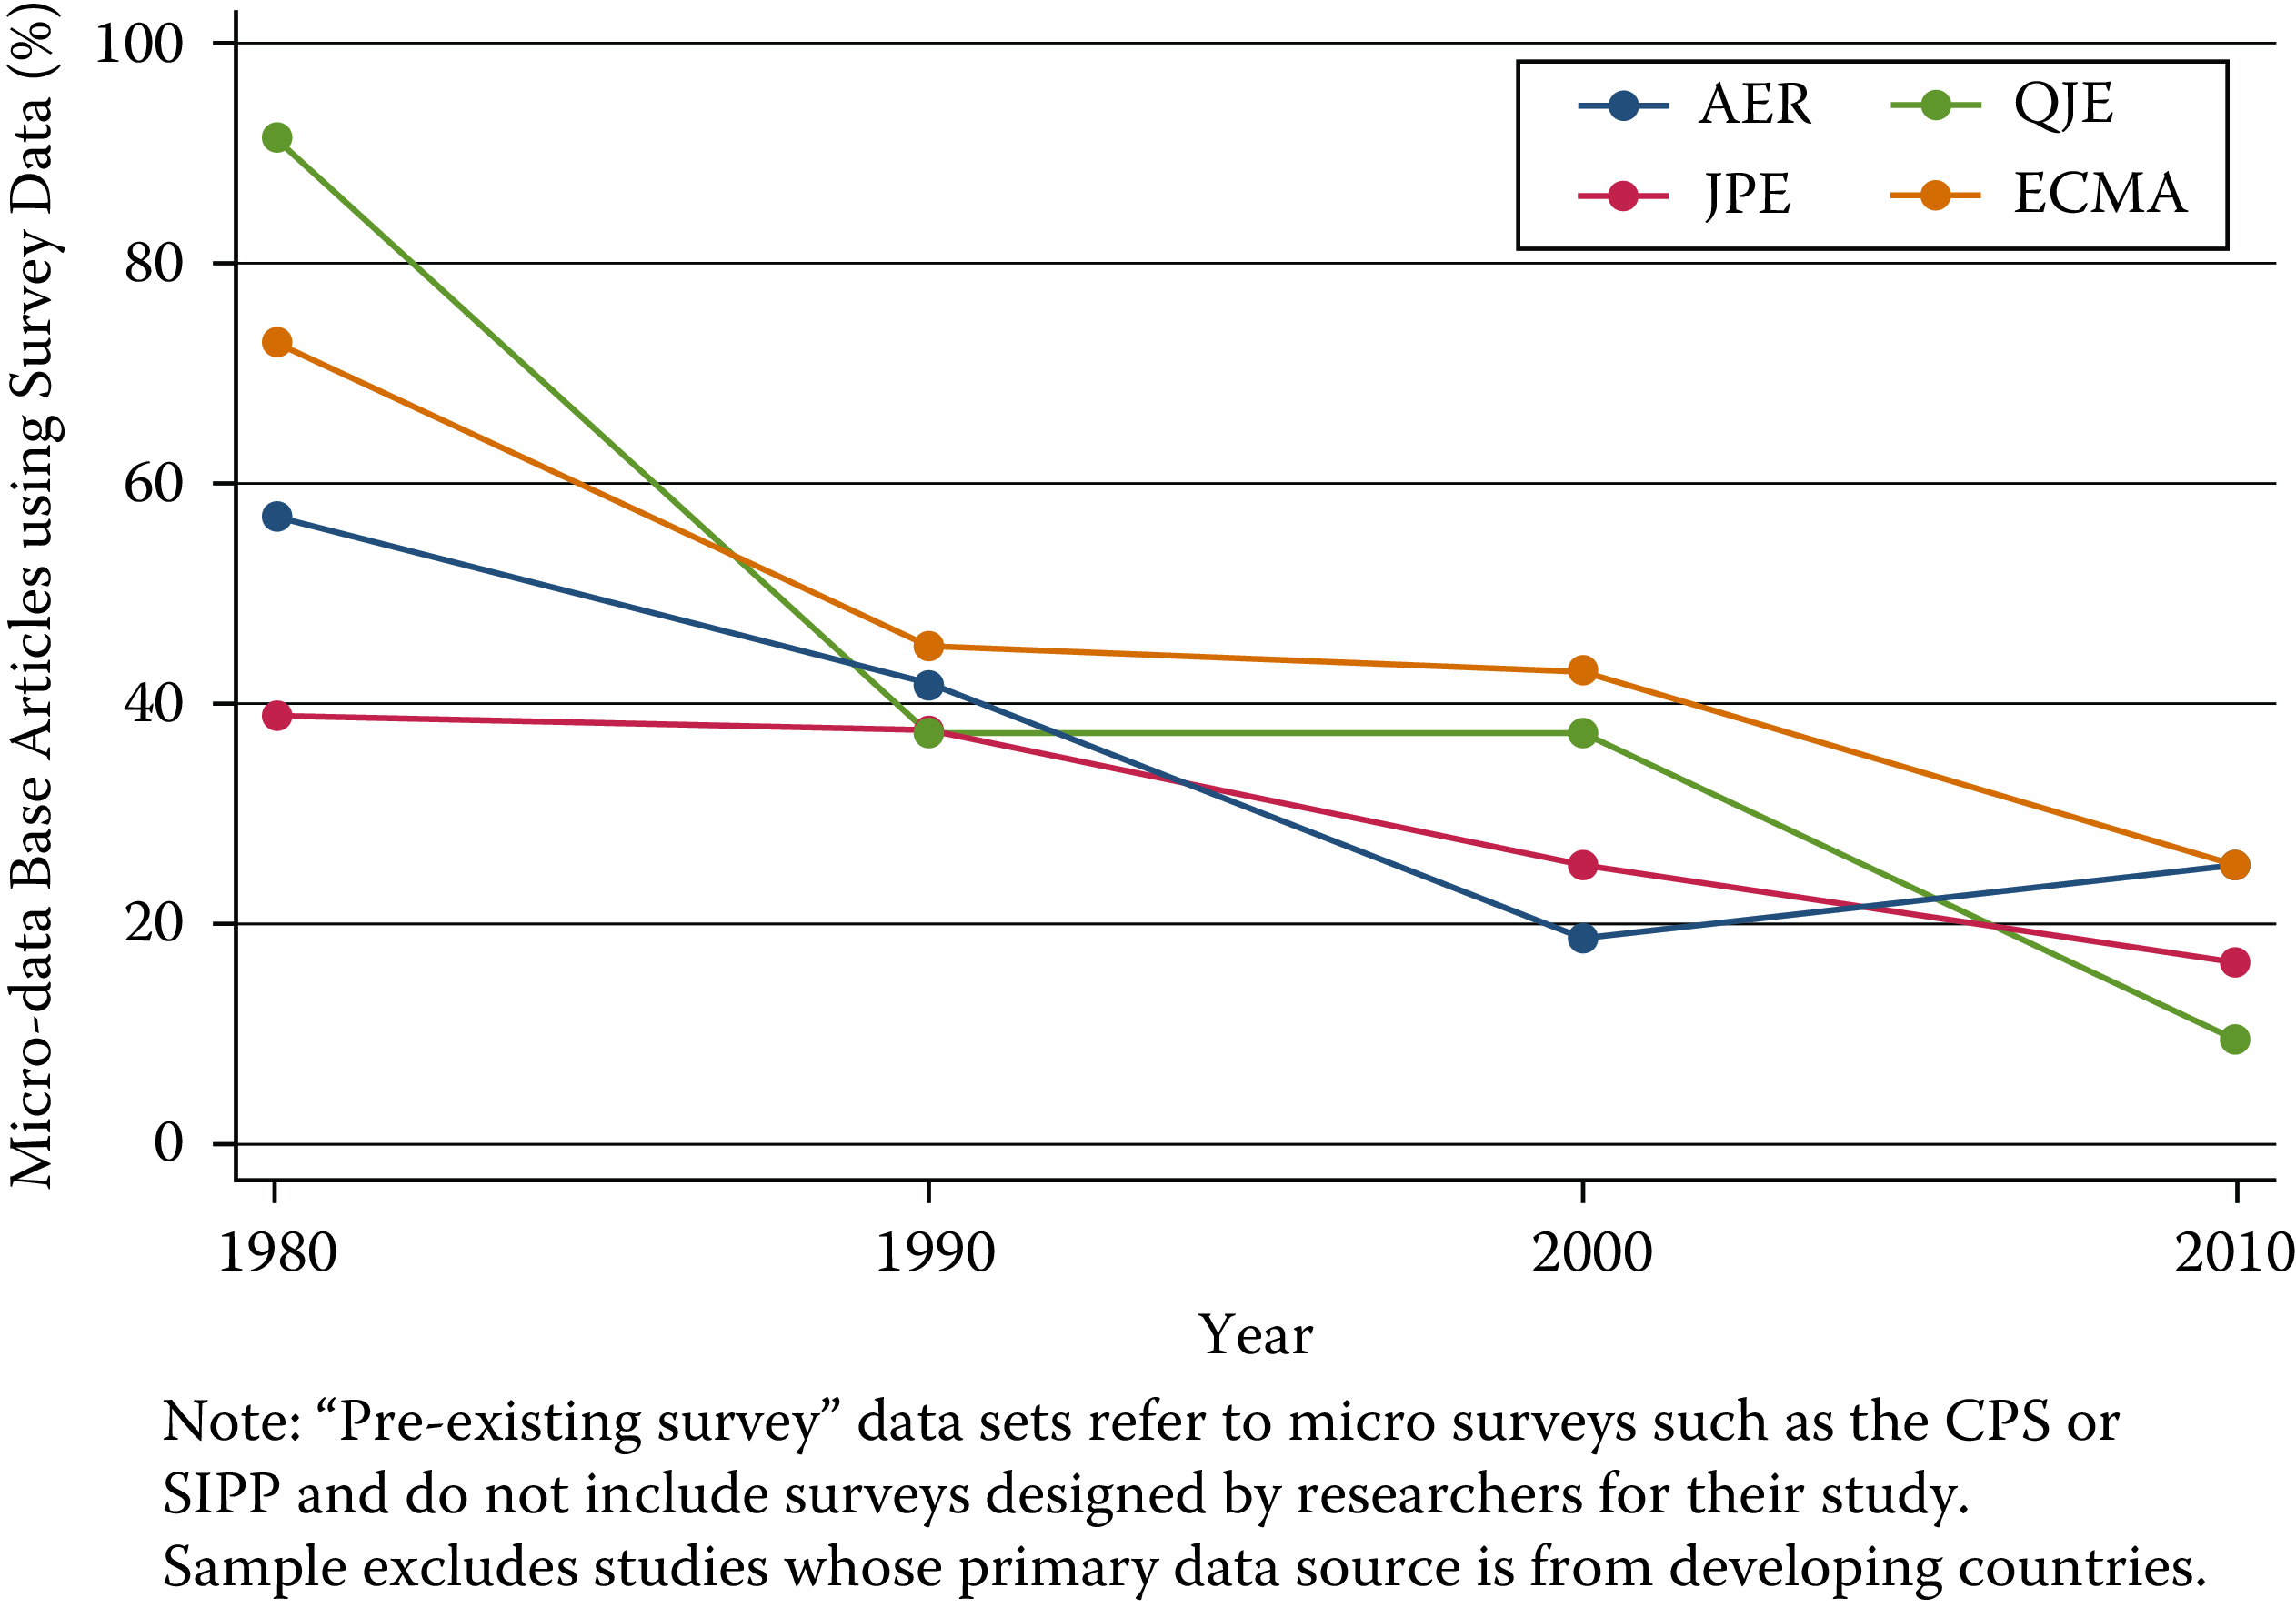
\includegraphics[width=0.7\linewidth]{ChapterIntro/figures/Figure1} 

}

\caption{Use of pre-existing survey data in publications in leading journals, 1980--2010 (@Chetty2012)}\label{fig:fig1}
\end{figure}

The way in which data are used has also changed for both government
agencies and businesses. Chief data officers are becoming as common in
federal and state governments as chief economists were decades ago, and
in cities like New York and Chicago, mayoral offices of data analytics
have the ability to provide rapid answers to important policy questions
(Lee et al. \protect\hyperlink{ref-lee2012rise}{2012}). But since
federal, state, and local agencies lack the capacity to do such analysis
themselves (Alawadhi et al.
\protect\hyperlink{ref-alawadhi2012building}{2012}), they must make
these data available either to consultants or to the research community.
Businesses are also learning that making effective use of their data
assets can have an impact on their bottom line (Brynjolfsson, Hitt, and
Kim \protect\hyperlink{ref-brynjolfsson2011strength}{2011}).

And the jobs have changed. The new job title of ``data scientist'' is
highlighted in job advertisements on CareerBuilder.com and
Burning-glass.com---in the same category as statisticians, economists,
and other quantitative social scientists if starting salaries are useful
indicators.

The goal of this book is to provide social scientists with an
understanding of the key elements of this new science, its value, and
the opportunities for doing better work. The goal is also to identify
the many ways in which the analytical toolkits possessed by social
scientists can be brought to bear to enhance the generalizability of the
work done by computer scientists.

We take a pragmatic approach, drawing on our experience of working with
data. Most social scientists set out to solve a real-world social or
economic problem: they frame the problem, identify the data, do the
analysis, and then draw inferences. At all points, of course, the social
scientist needs to consider the ethical ramifications of their work,
particularly respecting privacy and confidentiality. The book follows
the same structure. We chose a particular problem---the link between
research investments and innovation---because that is a major social
science policy issue, and one in which social scientists have been
addressing using big data techniques. While the example is specific and
intended to show how abstract concepts apply in practice, the approach
is completely generalizable. The web scraping, linkage, classification,
and text analysis methods on display here are canonical in nature. The
inference and privacy and confidentiality issues are no different than
in any other study involving human subjects, and the communication of
results through visualization is similarly generalizable.

\section{Defining big data and its value}\label{sec:1-2}

There are almost as many definitions of big data as there are new types
of data. One approach is to define big data as \emph{anything too big to
fit onto your computer}\footnote{This topic is discussed in more detail
  in Chapter 5}. Another approach is to define it as data with high
volume, high velocity, and great variety. We choose the description
adopted by the American Association of Public Opinion Research: ``The
term `Big Data' is an imprecise description of a rich and complicated
set of characteristics, practices, techniques, ethical issues, and
outcomes all associated with data'' (Japec et al.
\protect\hyperlink{ref-japec2015big}{2015}).

The value of the new types of data for social science is quite
substantial. Personal data has been hailed as the ``new oil'' of the
twenty-first century, and the benefits to policy, society, and public
opinion research are undeniable (Greenwood et al.
\protect\hyperlink{ref-greenwood2014}{2014}). Policymakers have found
that detailed data on human beings can be used to reduce crime, improve
health delivery, and manage cities better (Keller, Koonin, and Shipp
\protect\hyperlink{ref-keller2012big}{2012}). The scope is broad indeed:
one of this book's editors has used such data to not only help win
political campaigns but also show its potential for public policy.
Society can gain as well---recent work shows data-driven businesses were
5\% more productive and 6\% more profitable than their
competitors(Brynjolfsson, Hitt, and Kim
\protect\hyperlink{ref-brynjolfsson2011strength}{2011}). In short, the
vision is that social science researchers can potentially, by using data
with high velocity, variety, and volume, increase the scope of their
data collection efforts while at the same time reducing costs and
respondent burden, increasing timeliness, and increasing
precision(Murphy et al. \protect\hyperlink{ref-murphy2014social}{2014}).

\begin{center}\rule{0.5\linewidth}{\linethickness}\end{center}

\textbf{Example: New data enable new analyses}

Spotshotter data, which have fairly detailed information for each
gunfire incident, such as the precise timestamp and the nearest address,
as well as the type of shot, can be used to improve crime data (Carr and
Doleac \protect\hyperlink{ref-carr2015geography}{2015}); Twitter data
can be used to improve predictions around job loss, job gain, and job
postings (Antenucci et al.
\protect\hyperlink{ref-antenucci2014using}{2014}); and eBay postings can
be used to estimate demand elasticities (Einav and Levin
\protect\hyperlink{ref-einav2013data}{2013}).

\begin{center}\rule{0.5\linewidth}{\linethickness}\end{center}

But most interestingly, the new data can change the way we think about
measuring and making inferences about behavior. For example, it enables
the capture of information on the subject's entire environment---thus,
for example, the effect of fast food caloric labeling in health
interventions (Elbel, Gyamfi, and Kersh
\protect\hyperlink{ref-Elbel2011}{2011}); the productivity of a cashier
if he is within eyesight of a highly productive cashier but not
otherwise (Mas and Moretti \protect\hyperlink{ref-Mas2009}{2009}). So it
offers the potential to understand the effects of complex environmental
inputs on human behavior. In addition, big data, by its very nature,
enables us to study the tails of a distribution in a way that is not
possible with small data. Much of interest in human behavior is driven
by the tails of the distribution---health care costs by small numbers of
ill people (Stanton and Rutherford
\protect\hyperlink{ref-stanton2006high}{2006}), economic activity and
employment by a small number of firms (Evans
\protect\hyperlink{ref-evans1987tests}{1987}; Decker et al. to
appear)---and is impossible to study with the small sample sizes
available to researchers.

Instead we are still faced with the same challenges and responsibilities
as we were before in the survey and small data collection environment.
Indeed, social scientists have a great deal to offer to a (data) world
that is currently looking to computer scientists to provide answers. Two
major areas to which social scientists can contribute, based on decades
of experience and work with end users, are inference and attention to
data quality.

\section{Social science, inference, and big data}\label{sec:1.3}

The goal of empirical social science is to make inferences about a
population from available data. That requirement exists regardless of
the data source---and is a guiding principle for this book. For
probability-based survey data, methodology has been developed to
overcome problems in the data generating process. A guiding principle
for survey methodologists is the total survey error framework, and
statistical methods for weighting, calibration, and other forms of
adjustment are commonly used to mitigate errors in the survey process.
Likewise for ``broken'' experimental data, techniques like propensity
score adjustment and principal stratification are widely used to fix
flaws in the data generating process. Two books provide frameworks for
\emph{survey quality}\footnote{This topic is discussed in more detail in
  Chapter 10.}(Groves \protect\hyperlink{ref-groves2004survey}{2004};
Biemer and Lyberg \protect\hyperlink{ref-biemer2003}{2003}).

Across the social sciences, including economics, public policy,
sociology, management, (parts of) psychology and the like, we can
identify three categories of analysis with three different inferential
goals: description, causation, and prediction.

\textbf{Description}

The job of many social scientists is to provide descriptive statements
about the population of interest. These could be univariate, bivariate,
or even multivariate statements. \protect\hyperlink{chap:ml}{Machine
Learning} on machine learning will cover methods that go beyond simple
descriptive statistics, known as \emph{unsupervised learning} methods.

Descriptive statistics are usually created based on census data or
sample surveys to generate some summary statistics like a mean, median,
or a graphical distribution to describe the population of interest. In
the case of a census, the work ends right there. With sample surveys the
point estimates come with measures of uncertainties (standard errors).
The estimation of standard errors has been worked out for most
descriptive statistics and most common survey designs, even complex ones
that include multiple layers of sampling and disproportional selection
probabilities (Hansen, Hurwitz, and Madow
\protect\hyperlink{ref-hansen1993sample}{1993}; Valliant, Dever, and
Kreuter \protect\hyperlink{ref-valliant2013practical}{2013}).

\begin{center}\rule{0.5\linewidth}{\linethickness}\end{center}

\textbf{Example: Descriptive statistics}

The US Bureau of Labor Statistics surveys about 60,000 households a
month and from that survey is able to describe national employment and
unemployment levels. For example, in November 2015, total nonfarm
payroll employment increased by 211,000 in November, and the
unemployment rate was unchanged at 5.0\%. Job gains occurred in
construction, professional and technical services, and health care.
Mining and information lost jobs (Bureau of Labor Statistics
\protect\hyperlink{ref-BLS2015}{2015}).

\begin{center}\rule{0.5\linewidth}{\linethickness}\end{center}

Proper inference, even for purely descriptive purposes, from a sample to
the population rests usually on knowing that everyone from the target
population had the chance to be included in the survey, and knowing the
selection probability for each element in the population. The latter
does not necessarily need to be known prior to sampling, but eventually
a probability is assigned for each case. Getting the selection
probabilities right is particularly important when reporting totals
(Lohr \protect\hyperlink{ref-lohr2009sampling}{2009}). Unfortunately in
practice, samples that start out as probability samples can suffer from
a high rate of nonresponse. Because the survey designer cannot
completely control which units respond, the set of units that ultimately
respond cannot be considered to be a probability sample (Meyer, Mok, and
Sullivan \protect\hyperlink{ref-Meyer2015}{2015}). Nevertheless,
starting with a probability sample provides some degree of comfort that
a sample will have limited coverage errors (nonzero probability of being
in the sample), and there are methods for dealing with a variety of
missing data problems (Little and Rubin
\protect\hyperlink{ref-little2014statistical}{2014}).

\textbf{Causation}

In many cases, social scientists wish to test hypotheses, often
originating in theory, about relationships between phenomena of
interest. Ideally such tests stem from data that allow causal inference:
typically randomized experiments or strong nonexperimental study
designs. When examining the effect of \(X\) on \(Y\), knowing how cases
were selected into the sample or data set is much less important in the
estimation of causal effects than for descriptive studies, for example,
population means. What is important is that all elements of the
inferential population have a chance of being selected for the treatment
(Imbens and Rubin \protect\hyperlink{ref-imbens2015causal}{2015}). In
the debate about probability and nonprobability surveys, this
distinction is often overlooked. Medical researchers have operated with
unknown study selection mechanisms for years: for example, randomized
trials that enroll only selected samples.

\begin{center}\rule{0.5\linewidth}{\linethickness}\end{center}

\textbf{Example: New data and causal inference}

One of the major risks with using big data without thinking about the
data source is the misallocation of resources. Overreliance on, say,
Twitter data in targeting resources after hurricanes can lead to the
misallocation of resources towards young, Internet-savvy people with
cell phones, and away from elderly or impoverished neighborhoods
(Shelton et al. \protect\hyperlink{ref-shelton2014mapping}{2014}). Of
course, all data collection approaches have had similar risks. Bad
survey methodology led the \emph{Literary Digest} to incorrectly call
the 1936 election (Squire \protect\hyperlink{ref-squire19881936}{1988}).
Inadequate understanding of coverage, incentive and quality issues,
together with the lack of a comparison group, has hampered the use of
administrative records---famously in the case of using administrative
records on crime to make inference about the role of death penalty
policy in crime reduction (Donohue III and Wolfers
\protect\hyperlink{ref-donohue2006uses}{2006}).

\begin{center}\rule{0.5\linewidth}{\linethickness}\end{center}

Of course, in practice it is difficult to ensure that results are
generalizable, and there is always a concern that the treatment effect
on the treated is different than the treatment effect in the full
population of interest (Stuart
\protect\hyperlink{ref-stuart2010matching}{2010}). Having unknown study
selection probabilities makes it even more difficult to estimate
population causal effects, but substantial progress is being made
(DuGoff, Schuler, and Stuart
\protect\hyperlink{ref-dugoff2014generalizing}{2014}; Morgan and Winship
\protect\hyperlink{ref-morgan2014counterfactuals}{2014}). As long as we
are able to model the selection process, there is no reason not to do
causal inference from so-called nonprobability data.

\textbf{Prediction}

Forecasting or prediction tasks are a little less common among applied
social science researchers as a whole, but are certainly an important
element for users of official statistics---in particular, in the context
of social and economic indicators---as generally for decision-makers in
government and business. Here, similar to the causal inference setting,
it is of utmost importance that we do know the process that generated
the data, and we can rule out any unknown or unobserved systematic
selection mechanism.

\begin{center}\rule{0.5\linewidth}{\linethickness}\end{center}

\textbf{Example: Learning from the flu}

``Five years ago in 2009, a team of researchers from Google announced a
remarkable achievement in one of the world's top scientific journals,
\emph{Nature}. Without needing the results of a single medical check-up,
they were nevertheless able to track the spread of influenza across the
US. What's more, they could do it more quickly than the Centers for
Disease Control and Prevention (CDC). Google's tracking had only a day's
delay, compared with the week or more it took for the CDC to assemble a
picture based on reports from doctors' surgeries. Google was faster
because it was tracking the outbreak by finding a correlation between
what people searched for online and whether they had flu symptoms.
\ldots{}

``Four years after the original \emph{Nature} paper was published,
\emph{Nature News} had sad tidings to convey: the latest flu outbreak
had claimed an unexpected victim: Google Flu Trends. After reliably
providing a swift and accurate account of flu outbreaks for several
winters, the theory-free, data-rich model had lost its nose for where
flu was going. Google's model pointed to a severe outbreak but when the
slow-and-steady data from the CDC arrived, they showed that Google's
estimates of the spread of flu-like illnesses were overstated by almost
a factor of two.

``The problem was that Google did not know---could not begin to
know---what linked the search terms with the spread of flu. Google's
engineers weren't trying to figure out what caused what. They were
merely finding statistical patterns in the data. They cared about
correlation rather than causation'' (Harford
\protect\hyperlink{ref-harford2014big}{2014}).

\begin{center}\rule{0.5\linewidth}{\linethickness}\end{center}

\section{Social science, data quality, and big data}\label{sec:1-5}

Most data in the real world are noisy, inconsistent, and suffers from
missing values, regardless of its source. Even if data collection is
cheap, the costs of creating high-quality data from the source --
\emph{cleaning, curating, standardizing, and integrating}\footnote{This
  topic is discussed in more detail in Chapter 3.} -- are substantial.

Data quality can be characterized in multiple ways (Christen
\protect\hyperlink{ref-christen2012data}{2012}\protect\hyperlink{ref-christen2012data}{b}):

\begin{itemize}
\item
  \textbf{Accuracy}: How accurate are the attribute values in the data?
\item
  \textbf{Completeness}: Is the data complete?
\item
  \textbf{Consistency}: How consistent are the values in and between the
  database(s)?
\item
  \textbf{Timeliness}: How timely is the data?
\item
  \textbf{Accessibility}: Are all variables available for analysis?
\end{itemize}

Social scientists have decades of experience in transformingmessy,
noisy, and unstructured data into a well-defined, clearly structured,
and quality-tested data set. Preprocessing is a complex and
time-consuming process because it is ``hands-on''---it requires judgment
and cannot be effectively automated. A typical workflow comprises
multiple steps from data definition to parsing and ends with filtering.
It is difficult to overstate the value of preprocessing for any data
analysis, but this is particularly true in big data. Data need to be
parsed, standardized, deduplicated, and normalized.

\textbf{Parsing} is a fundamental step taken regardless of the data
source, and refers to the decomposition of a complex variable into
components. For example, a freeform address field like ``1234 E 56th
St'' might be broken down into a street number ``1234'' and a street
name ``E 56th St.'' The street name could be broken down further to
extract the cardinal direction ``E'' and the designation ``St.'' Another
example would be a combined full name field that takes the form of a
comma-separated last name, first name, and middle initial as in
``Miller, David A.'' Splitting these identifiers into components permits
the creation of more refined variables that can be used in the matching
step.

In the simplest case, the distinct parts of a character field are
delimited. In the name field example, it would be easy to create the
separate fields ``Miller'' and ``David A'' by splitting the original
field at the comma. In more complex cases, special code will have to be
written to parse the field. Typical steps in a parsing procedure
include:

\begin{enumerate}
\def\labelenumi{\arabic{enumi}.}
\item
  Splitting fields into tokens (words) on the basis of delimiters,
\item
  Standardizing tokens by lookup tables and substitution by a standard
  form,
\item
  Categorizing tokens,
\item
  Identifying a pattern of anchors, tokens, and delimiters,
\item
  Calling subroutines according to the identified pattern, therein
  mapping of tokens to the predefined components.
\end{enumerate}

\textbf{Standardization} refers to the process of simplifying data by
replacing variant representations of the same underlying observation by
a default value in order to improve the accuracy of field comparisons.
For example, ``First Street'' and ``1st St'' are two ways of writing the
same street name, but a simple string comparison of these values will
return a poor result. By standardizing fields---and using the same
standardization rules across files!---the number of true matches that
are wrongly classified as nonmatches (i.e., the number of false
nonmatches) can be reduced.

Some common examples of standardization are:

\begin{itemize}
\item
  Standardization of different spellings of frequently occurring words:
  for example, replacing common abbreviations in street names (Ave, St,
  etc.) or titles (Ms, Dr, etc.) with a common form. These kinds of
  rules are highly country- and language-specific.
\item
  General standardization, including converting character fields to all
  uppercase and removing punctuation and digits.
\end{itemize}

\textbf{Deduplication} consists of removing redundant records from a
single list, that is, multiple records from the same list that refer to
the same underlying entity. After deduplication, each record in the
first list will have at most one true match in the second list and vice
versa. This simplifies the record linkage process and is necessary if
the goal of record linkage is to find the best set of one-to-one links
(as opposed to a list of all possible links). One can deduplicate a list
by applying record linkage techniques described in this chapter to link
a file to itself.

\textbf{Normalization} is the process of ensuring that the fields that
are being compared across files are as similar as possible in the sense
that they could have been generated by the same process. At minimum, the
same standardization rules should be applied to both files. For
additional examples, consider a salary field in a survey. There are
number different ways that salary could be recorded: it might be
truncated as a privacy-preserving measure or rounded to the nearest
thousand, and missing values could be imputed with the mean or with
zero. During normalization we take note of exactly how fields are
recorded.

\section{New tools for new data}\label{new-tools-for-new-data}

The new data sources that we have discussed frequently require working
at scales for which the social scientist's familiar tools are not
designed. Fortunately, the wider research and data analytics community
has developed a wide variety of often more scalable and flexible
tools---tools that we will introduce within this book.

Relational database management systems (DBMSs)\footnote{This topic is
  discussed in more detail in Chapter 4.} are used throughout business
as well as the sciences to organize, process, and search large
collections of structured data. NoSQL DBMSs are used for data that is
extremely large and/or unstructured, such as collections of web pages,
social media data (e.g., Twitter messages), and clinical notes.
Extensions to these systems and also specialized single-purpose DBMSs
provide support for data types that are not easily handled in
statistical packages such as geospatial data, networks, and graphs.

Open source programming systems such as Python (used extensively
throughout this book) and R provide high-quality implementations of
numerous data analysis and visualization methods, from regression to
statistics, text analysis, network analysis, and much more. Finally,
parallel computing systems such as Hadoop and Spark can be used to
harness parallel computer clusters for extremely large data sets and
computationally intensive analyses.

These various components may not always work together as smoothly as do
integrated packages such as SAS, SPSS, and Stata, but they allow
researchers to take on problems of great scale and complexity.
Furthermore, they are developing at a tremendous rate as the result of
work by thousands of people worldwide. For these reasons, the modern
social scientist needs to be familiar with their characteristics and
capabilities.

\section{\texorpdfstring{The book's ``use
case''}{The book's use case}}\label{sec:1-6}

This book is about the uses of big data in social science. Our focus is
on working through the use of data as a social scientist normally
approaches research. That involves thinking through how to use such data
to address a question from beginning to end, and thereby learning about
the associated tools---rather than simply engaging in coding exercises
and then thinking about how to apply them to a potpourri of social
science examples.

There are many examples of the use of big data in social science
research, but relatively few that feature all the different aspects that
are covered in this book. As a result, the chapters in the book draw
heavily on a use case based on one of the first large-scale big data
social science data infrastructures. This infrastructure, based on
UMETRICS\footnote{UMETRICS: Universities Measuring the Impact of
  Research on Innovation and Science (Lane et al.
  \protect\hyperlink{ref-lane2015new}{2015})} data housed at the
University of Michigan's Institute for Research on Innovation and
Science (IRIS)\footnote{iris.isr.umich.edu} and enhanced with data from
the US Census Bureau, provides a new quantitative analysis and
understanding of science policy based on large-scale computational
analysis of new types of data.

The infrastructure was developed in response to a call from the
President's Science Advisor (Jack Marburger) for a \emph{science of
science policy} (Marburger
\protect\hyperlink{ref-marburger2005wanted}{2005}). He wanted a
scientific response to the questions that he was asked about the impact
of investments in science.

\begin{center}\rule{0.5\linewidth}{\linethickness}\end{center}

\textbf{Example: The Science of Science Policy}

Marburger wrote (Marburger
\protect\hyperlink{ref-marburger2005wanted}{2005}): ``How much should a
nation spend on science? What kind of science? How much from private
versus public sectors? Does demand for funding by potential science
performers imply a shortage of funding or a surfeit of performers? These
and related science policy questions tend to be asked and answered today
in a highly visible advocacy context that makes assumptions that are
deserving of closer scrutiny. A new `science of science policy' is
emerging, and it may offer more compelling guidance for policy decisions
and for more credible advocacy. \ldots{}

``Relating R\&D to innovation in any but a general way is a tall order,
but not a hopeless one. We need econometric models that encompass enough
variables in a sufficient number of countries to produce reasonable
simulations of the effect of specific policy choices. This need won't be
satisfied by a few grants or workshops, but demands the attention of a
specialist scholarly community. As more economists and social scientists
turn to these issues, the effectiveness of science policy will grow, and
of science advocacy too.''

\begin{center}\rule{0.5\linewidth}{\linethickness}\end{center}

Responding to this policy imperative is a tall order, because it
involves using all the social science and computer science tools
available to researchers. The new digital technologies can be used to
capture the links between the inputs into research, the way in which
those inputs are organized, and the subsequent outputs (Weinberg et al.
\protect\hyperlink{ref-weinberg2014science}{2014}; Zolas et al.
\protect\hyperlink{ref-zolas2015wrapping}{2015}). The social science
questions that are addressable with this data infrastructure include the
effect of research training on the placement and earnings of doctoral
recipients, how university trained scientists and engineers affect the
productivity of the firms they work for, and the return on investments
in research. Figure \ref{fig:fig2} provides an abstract representation
of the empirical approach that is needed: data about grants, the people
who are funded on grants, and the subsequent scientific and economic
activities.

First, data must be captured on what is funded, and since the data are
in text format, computational linguistics tools must be applied
(\protect\hyperlink{chap:text}{Text Analysis}). Second, data must be
captured on who is funded, and how they interact in teams, so network
tools and analysis must be used
(\protect\hyperlink{chap:networks}{Networks: The Basics}). Third,
information about the type of results must be gleaned from the web and
other sources (\protect\hyperlink{chap:web}{Working with Web Data and
APIs}).

Finally, the disparate complex data sets need to be stored in databases
(\protect\hyperlink{chap:db}{Databases}), integrated
(\protect\hyperlink{chap:link}{Record Linkage}), analyzed
(\protect\hyperlink{chap:ml}{Machine Learning}), and used to make
inferences ({[}Errors and Inference{]}).

\begin{figure}

{\centering 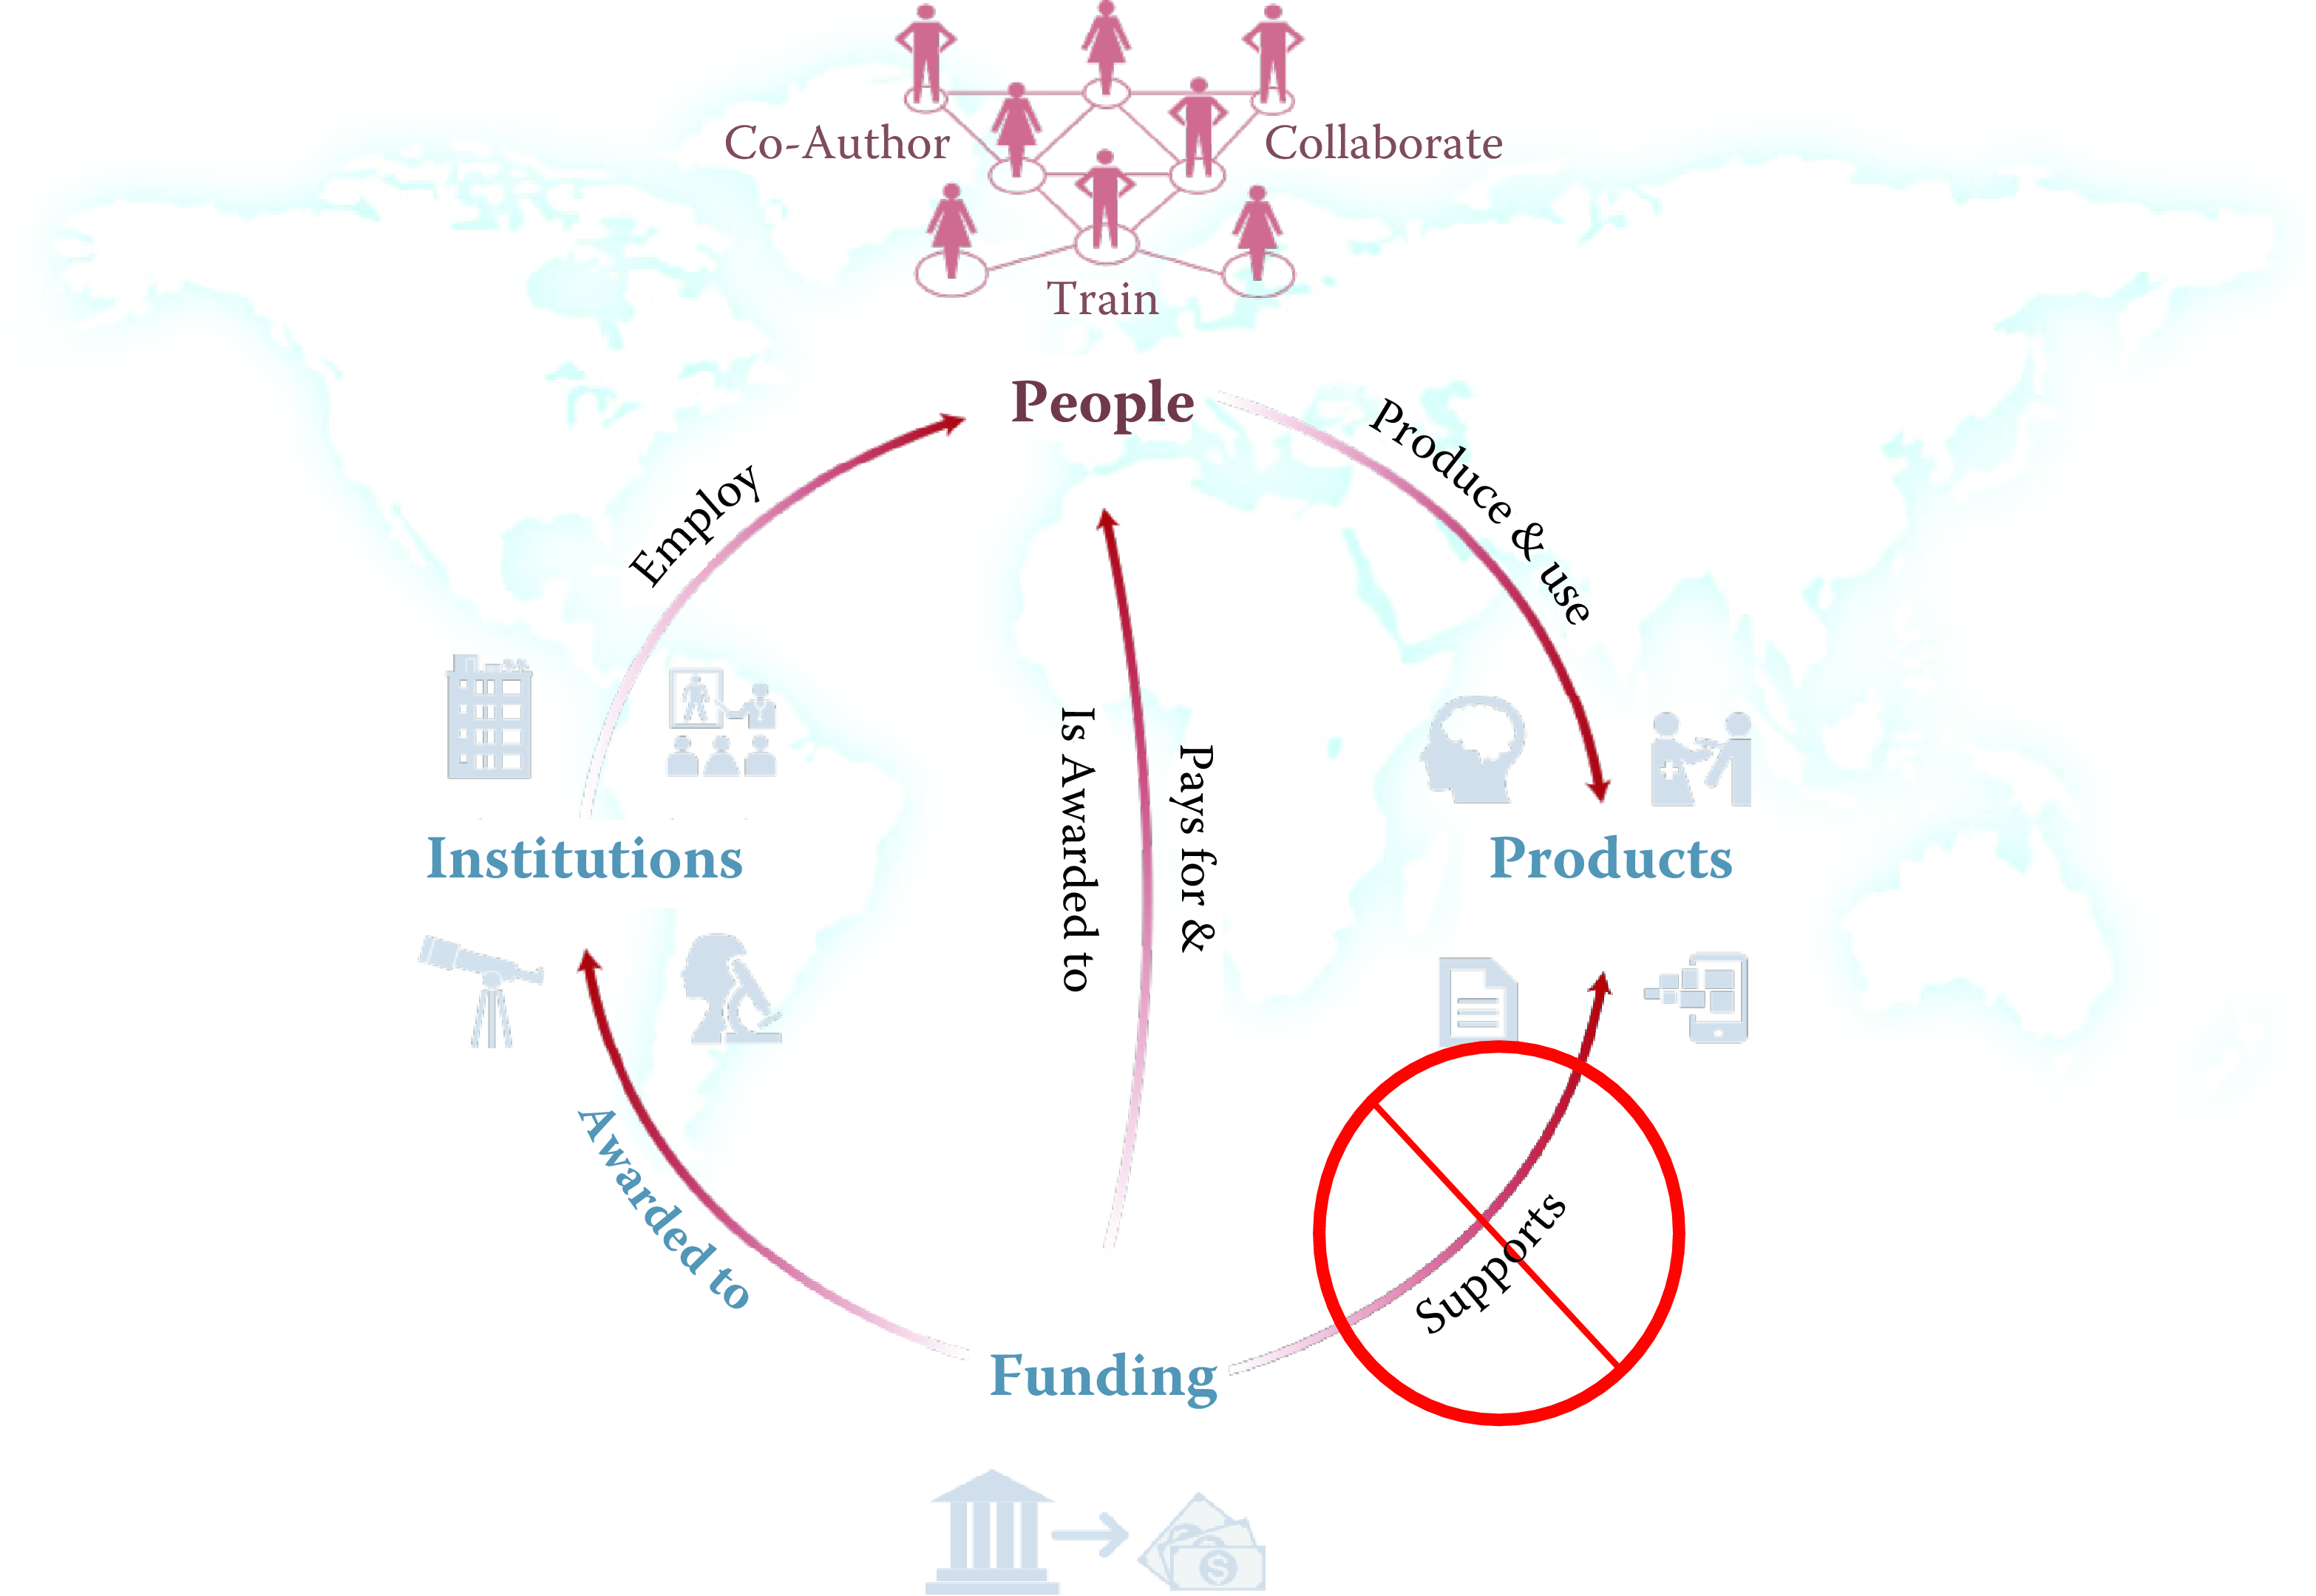
\includegraphics[width=0.7\linewidth]{ChapterIntro/figures/figure_cameron} 

}

\caption{A visualization of the complex links between what and who is funded, and the results; tracing the direct link between funding and results is misleading and wrong}\label{fig:fig2}
\end{figure}

The use case serves as the thread that ties many of the ideas together.
Rather than asking the reader to learn how to code ``hello world,'' we
build on data that have been put together to answer a real-world
question, and provide explicit examples based on that data. We then
provide examples that show how the approach generalizes.

For example, the text analysis chapter
(\protect\hyperlink{chap:text}{Text Analysis}) shows how to use natural
language processing to describe \emph{what} research is being done,
using proposal and award text to identify the research topics in a
portfolio (Talley et al.
\protect\hyperlink{ref-talley2011database}{2011}; Evans and Foster
\protect\hyperlink{ref-Evans2011}{2011}). But then it also shows how the
approach can be used to address a problem that is not just limited to
science policy---the conversion of massive amounts of knowledge that is
stored in text to usable information.

Similarly, the network analysis chapter
(\protect\hyperlink{chap:networks}{Networks: The Basics}) gives specific
examples using the UMETRICS data and shows how such data can be used to
create new units of analysis---the networks of researchers who do
science, and the networks of vendors who supply research inputs. It also
shows how networks can be used to study a wide variety of other social
science questions.

In another example, we use APIs\footnote{Application Programming
  Interfaces} provided by publishers to describe the results generated
by research funding in terms of publications and other measures of
scientific impact, but also provide code that can be repurposed for many
similar APIs.

And, of course, since all these new types of data are provided in a
variety of different formats, some of which are quite large (or
voluminous), and with a variety of different timestamps (or velocity),
we discuss how to store the data in different types of data formats.

\section{The structure of the book}\label{the-structure-of-the-book}

We organize the book in three parts, based around the way social
scientists approach doing research. The first set of chapters addresses
the new ways to capture, curate, and store data. The second set of
chapters describes what tools are available to process and classify
data. The last set deals with analysis and the appropriate handling of
data on individuals and organizations.

\begin{figure}

{\centering 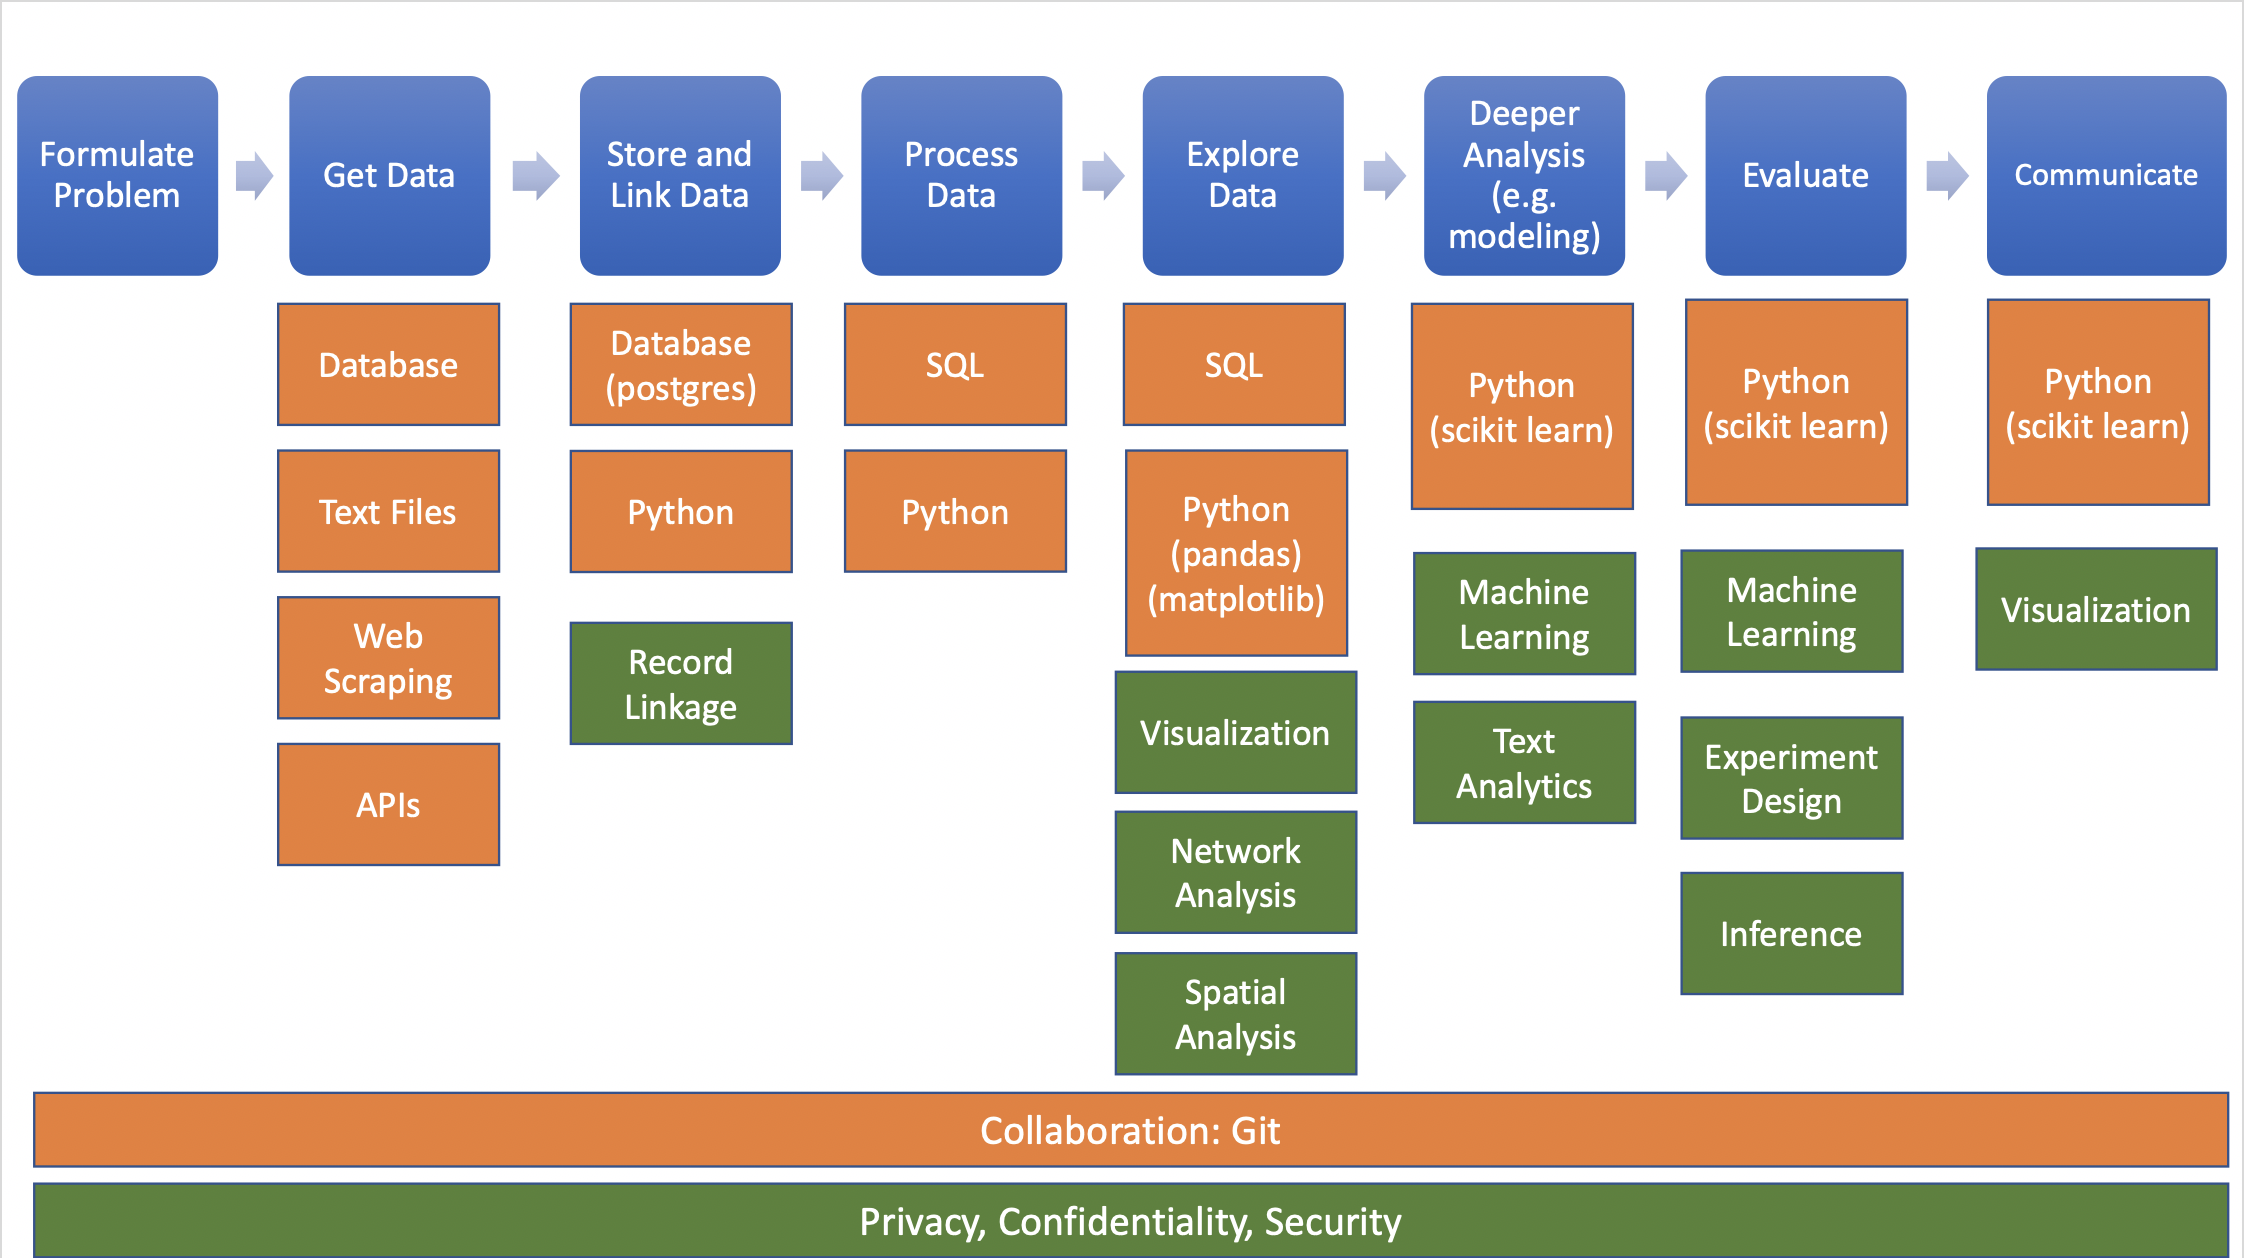
\includegraphics[width=1\linewidth]{ChapterIntro/figures/projectflow} 

}

\caption{The data science project workflow. Blue represents each step in the project, orange represents the tools used in that step, and green represents the methods for analysis.}\label{fig:projectfig}
\end{figure}

\subsection{Part I: Capture and
curation}\label{part-i-capture-and-curation}

The four chapters in Part I (see Figure \ref{fig:fig3}) tell you how to
capture and manage data.

\protect\hyperlink{chap:web}{Working with Web Data and APIs} describes
how to extract information from social media about the transmission of
knowledge. The particular application will be to develop links to
authors' articles on Twitter using PLOS articles and to pull information
about authors and articles from web sources by using an API. You will
learn how to retrieve link data from bookmarking services, citations
from Crossref, links from Facebook, and information from news coverage.
In keeping with the social science grounding that is a core feature of
the book, the chapter discusses what data can be captured from online
sources, what is potentially reliable, and how to manage data
qualityissues.

Big data differs from survey data in that we must typically combine data
from multiple sources to get a complete picture of the activities of
interest. Although computer scientists may sometimes simply ``mash''
data sets together, social scientists are rightfully concerned about
issues of missing links, duplicative links, and erroneous links.
\protect\hyperlink{chap:link}{Record Linkage} provides an overview of
traditional rule-based and probabilistic approaches to data linkage, as
well as the important contributions of machine learning to the linkage
problem.

Once data have been collected and linked into different files, it is
necessary to store and organize it. Social scientists are used to
working with one analytical file, often in statistical software tools
such as SAS or Stata. \protect\hyperlink{chap:db}{Databases}, which may
be the most important chapter in the book, describes different
approaches to storing data in ways that permit rapid and reliable
exploration andanalysis.

Big data is sometimes defined as data that are too big to fit onto the
analyst's computer. {[}Programming with Big Data{]} provides an overview
of clever programming techniques that facilitate the use of data (often
using parallel computing). While the focus is on one of the most widely
used big data programming paradigms and its most popular implementation,
Apache Hadoop, the goal of the chapter is to provide a conceptual
framework to the key challenges that the approach is designed to
address.

\begin{figure}

{\centering 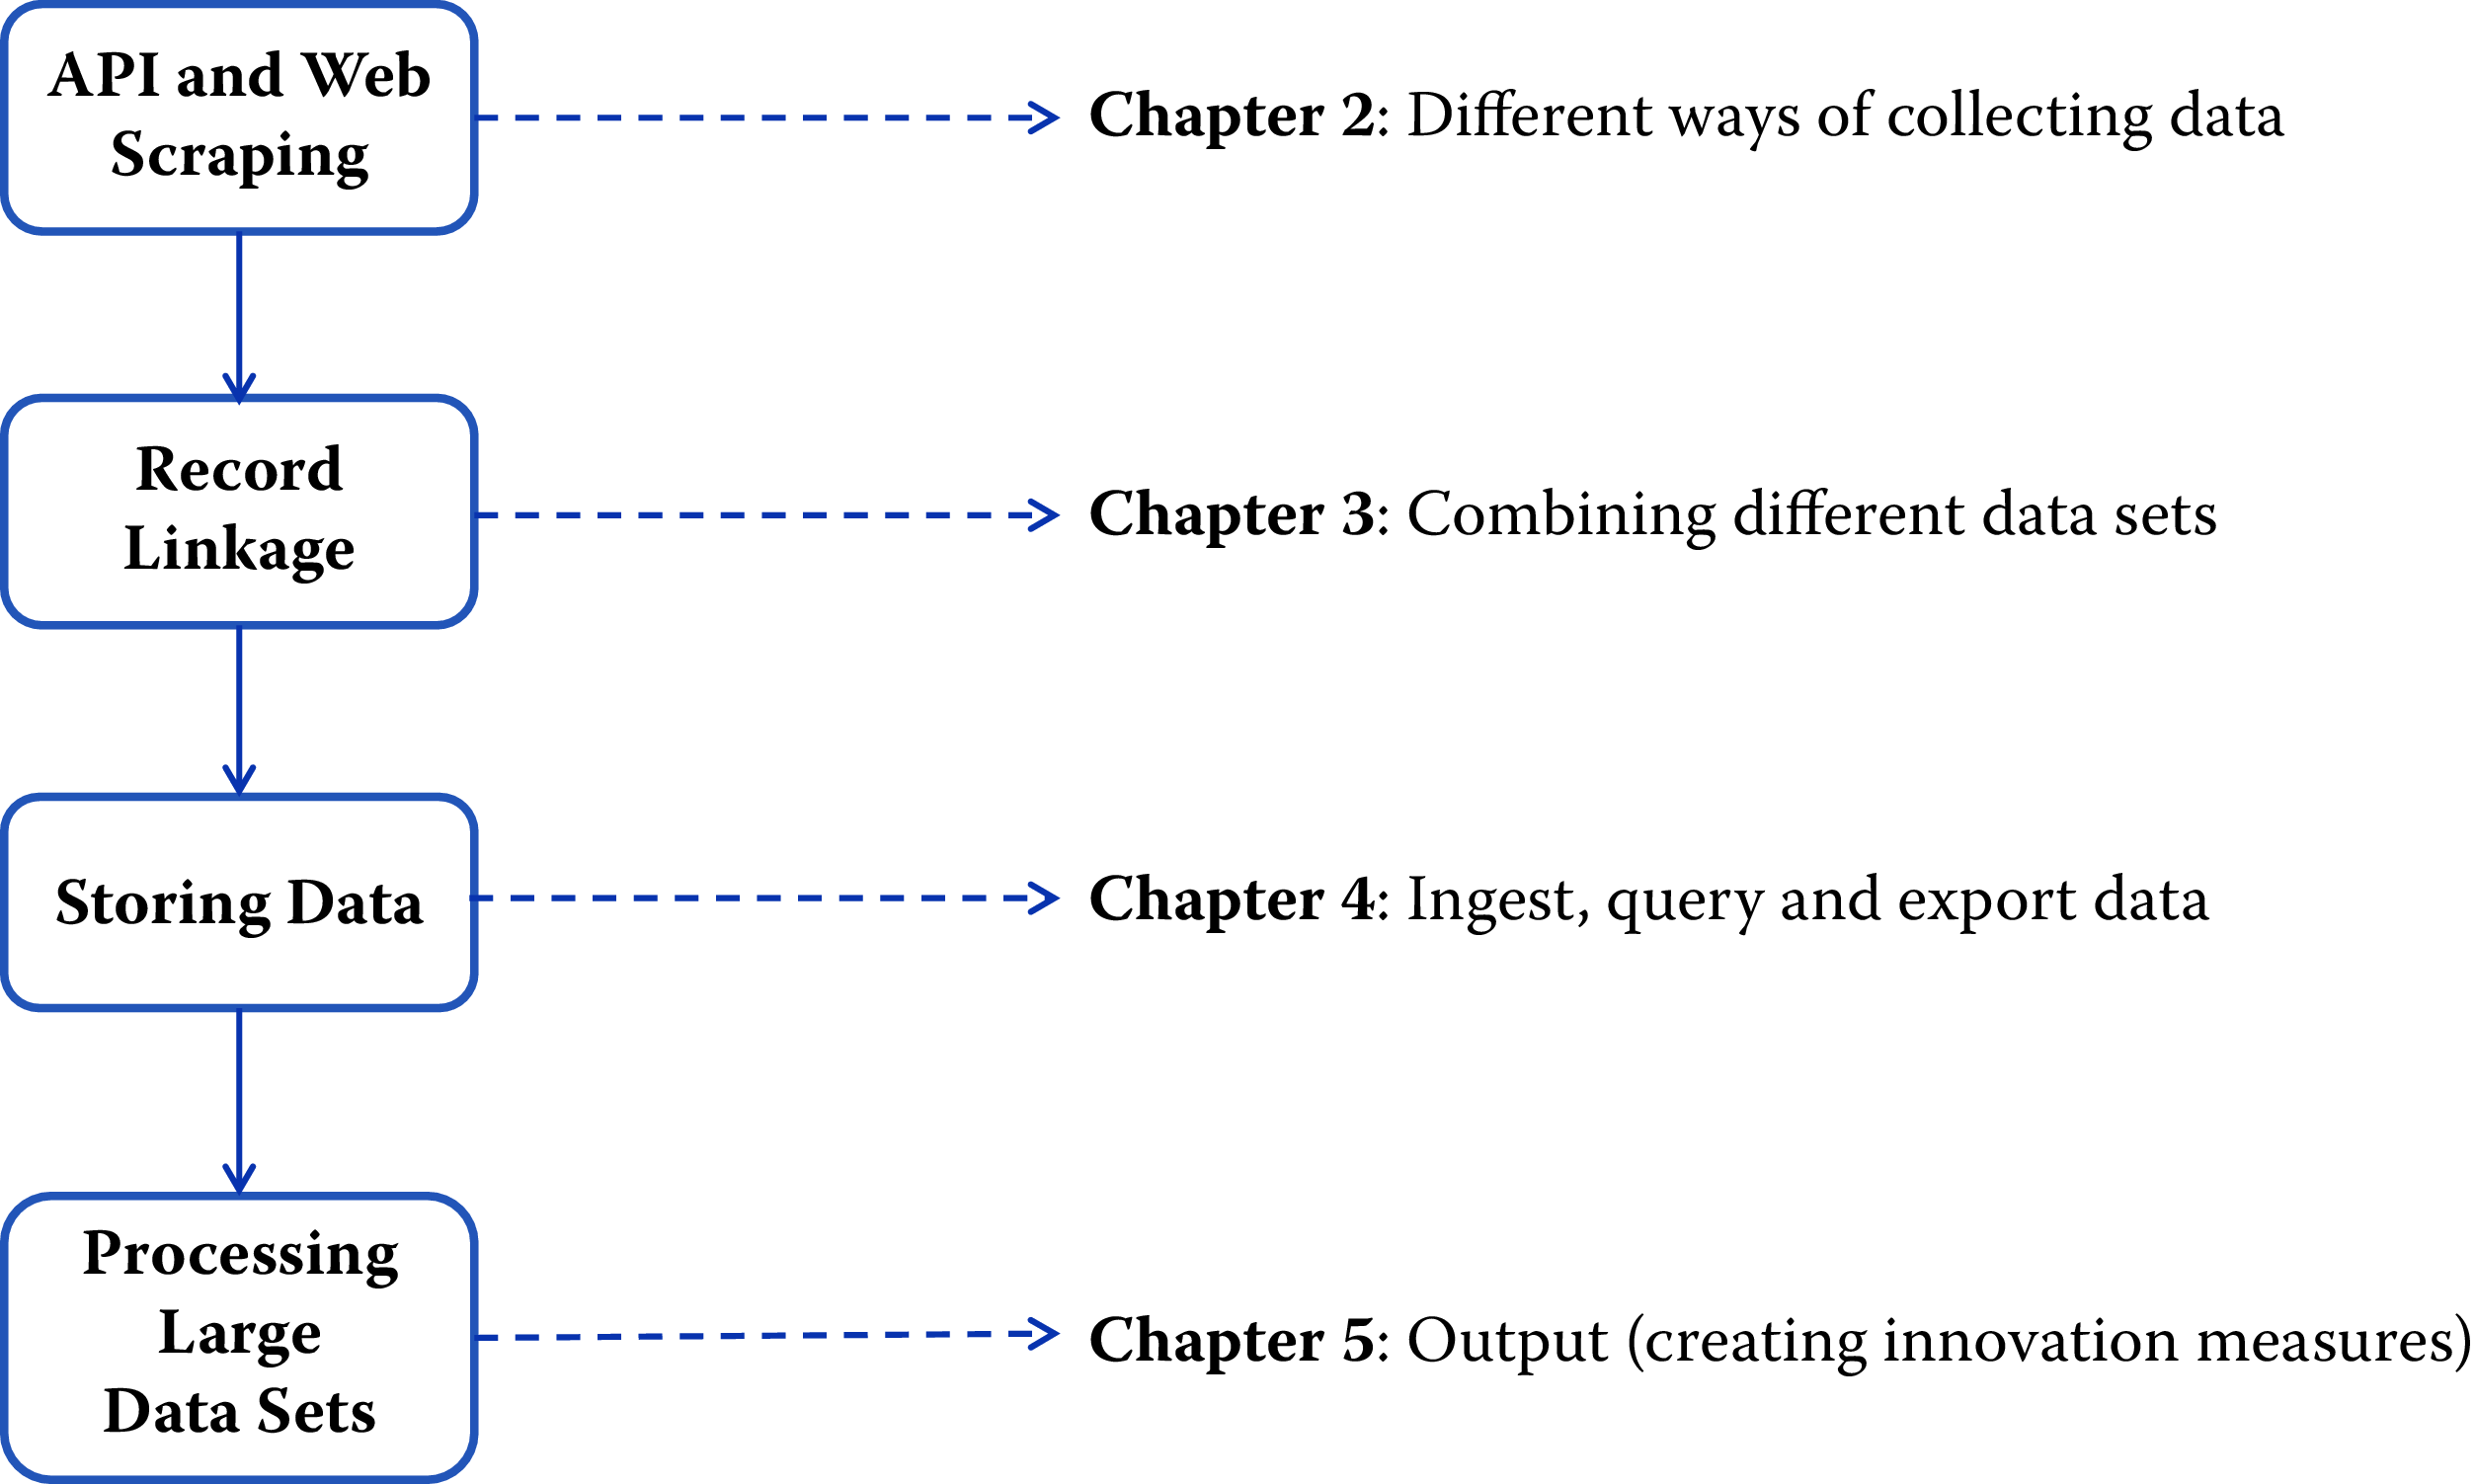
\includegraphics[width=0.7\linewidth]{ChapterIntro/figures/Figure2} 

}

\caption{The four chapters of Part I focus on *data capture* and *curation*}\label{fig:fig3}
\end{figure}

\subsection{Part II: Modeling and
analysis}\label{part-ii-modeling-and-analysis}

The three chapters in Part II (see Figure \ref{fig:fig4}) introduce
three of the most important tools that can be used by social scientists
to do new and exciting research: machine learning, text analysis, and
social network analysis.

\protect\hyperlink{chap:ml}{Machine Learning} introduces machine
learning methods. It shows the power of machine learning in a variety of
different contexts, particularly focusing on clustering and
classification. You will get an overview of basic approaches and how
those approaches are applied. The chapter builds from a conceptual
framework and then shows you how the different concepts are translated
into code. There is a particular focus on random forests and support
vector machine (SVM) approaches.

\protect\hyperlink{chap:text}{Text Analysis} describes how social
scientists can make use of one of the most exciting advances in big
data---text analysis. Vast amounts of data that are stored in documents
can now be analyzed andsearched so that different types of information
can be retrieved. Documents (and the underlying activities of the
entities that generated the documents) can be categorized into topics or
fields as well as summarized. In addition, machine translation can be
used to compare documents in different languages.

Social scientists are typically interested in describing the activities
of individuals and organizations (such as households and firms) in a
variety of economic and social contexts. The frames within which data
are collected have typically been generated from tax or other
programmatic sources. The new types of data permit new units of
analysis---particularly network analysis---largely enabled by advances
in mathematical graph theory. Thus,
\protect\hyperlink{chap:networks}{Networks: The Basics} describes how
social scientists can use network theory to generate measurable
representations of patterns of relationships connecting entities. As the
author points out, the value of the new framework is not only in
constructing different right-hand-side variables but also in studying an
entirely new unit of analysis that lies somewhere between the largely
atomistic actors that occupy the markets of neo-classical theory and the
tightly managed hierarchies that are the traditional object of inquiry
of sociologists and organizational theorists.

\begin{figure}

{\centering 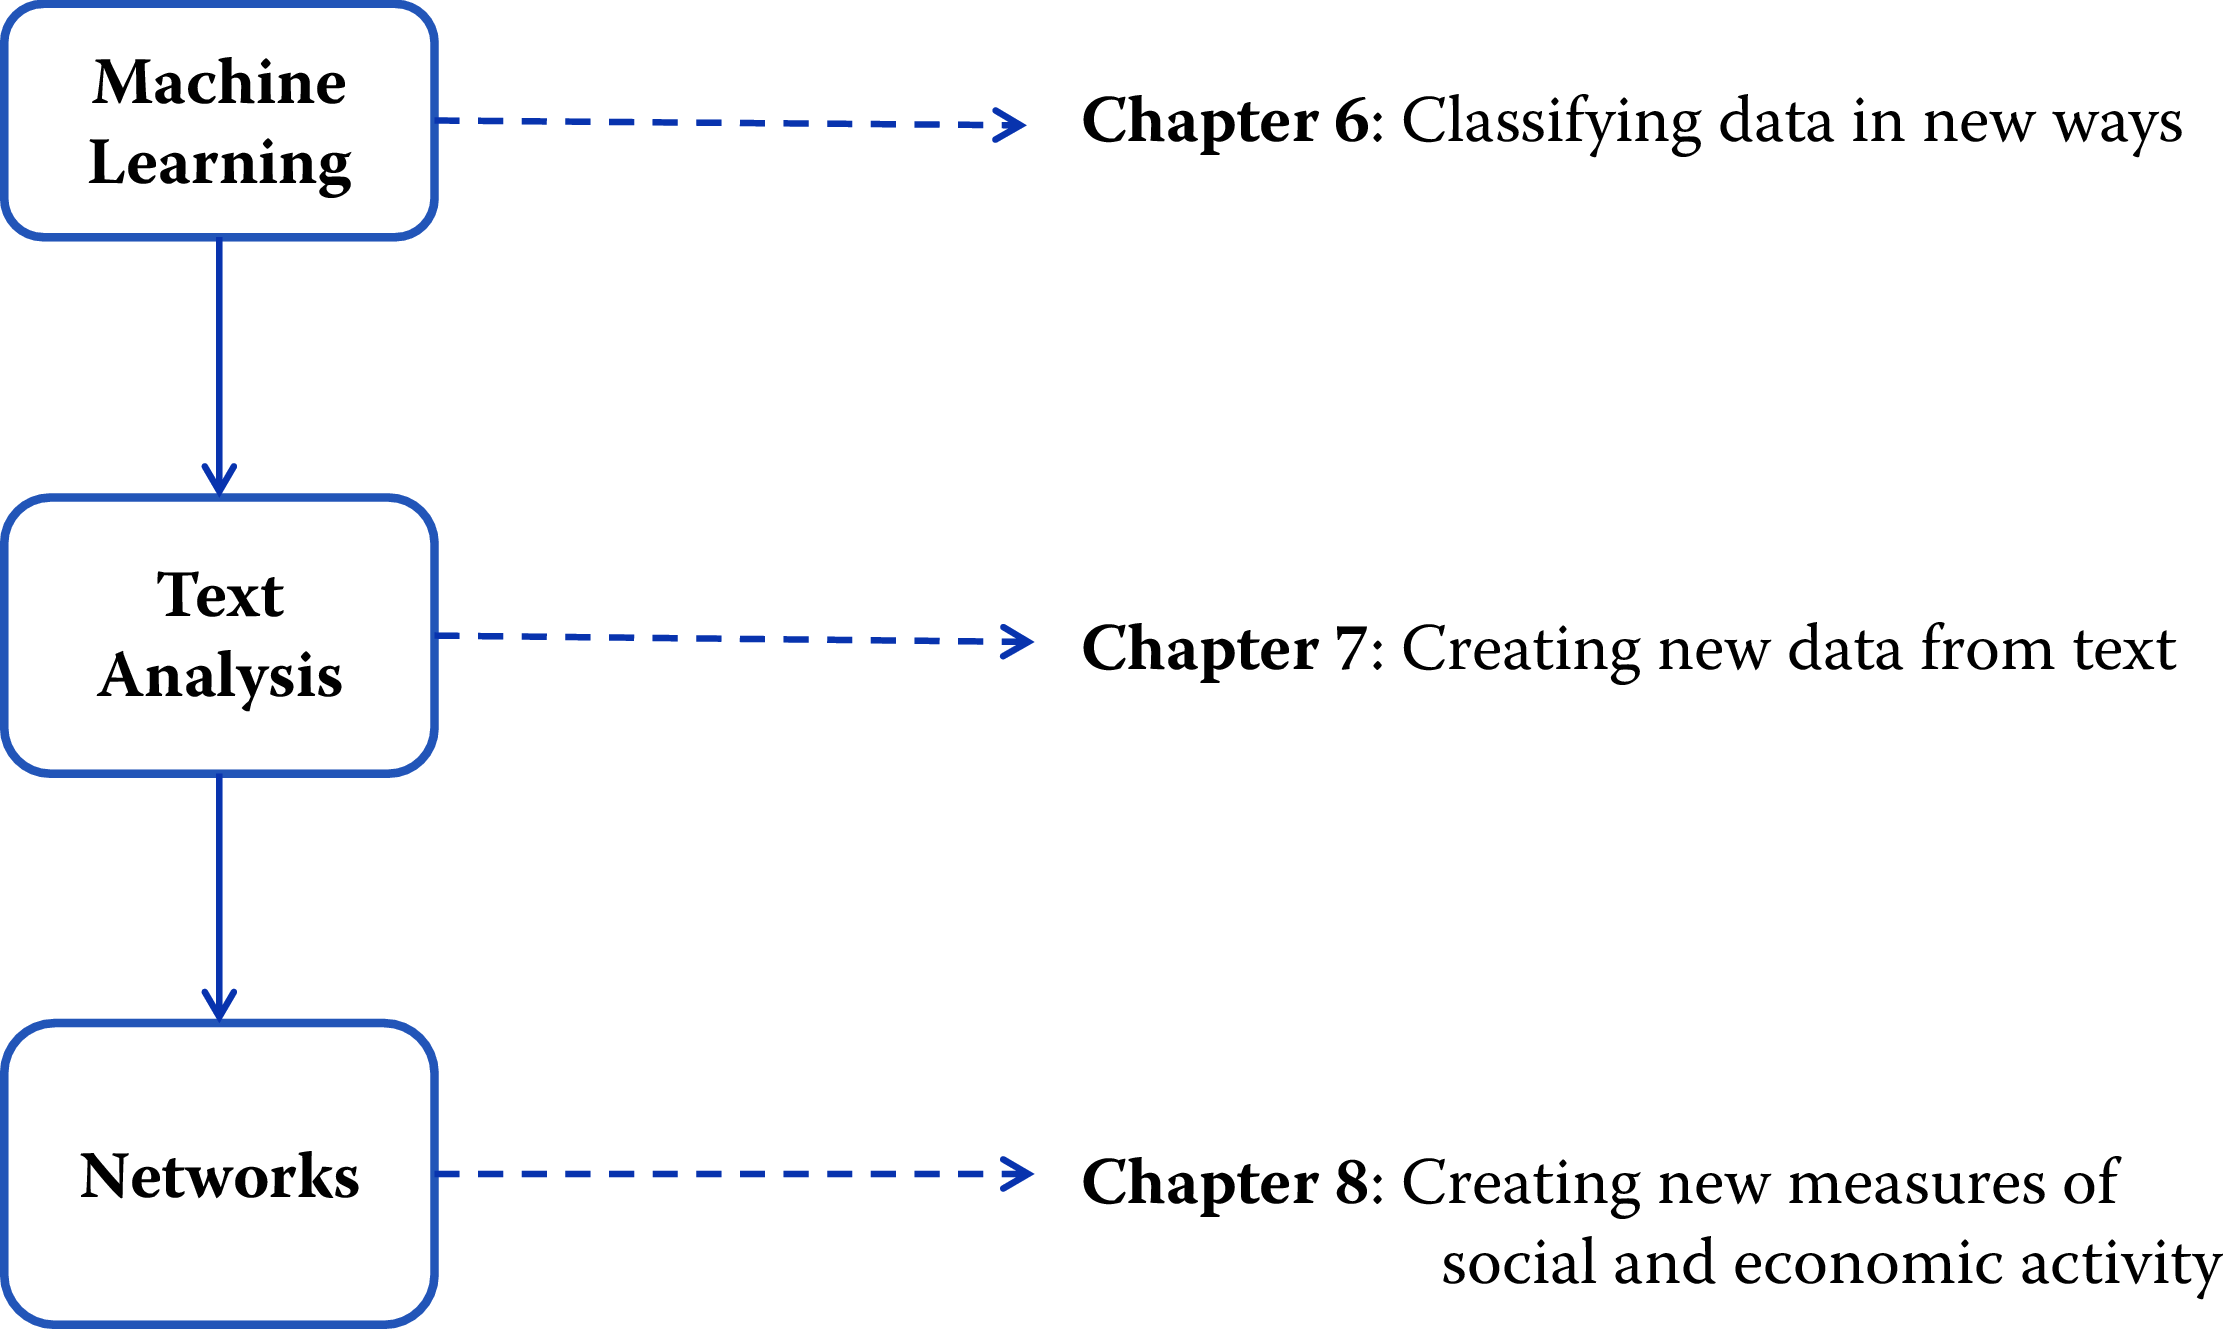
\includegraphics[width=0.7\linewidth]{ChapterIntro/figures/Figure3} 

}

\caption{The four chapters in Part II focus on data *modeling* and *analysis*}\label{fig:fig4}
\end{figure}

\subsection{Part III: Inference and
ethics}\label{part-iii-inference-and-ethics}

The four chapters in Part III (see Figure \ref{fig:fig5}) cover three
advanced topics relating to data inference and ethics---information
visualization, errors and inference, and privacy and
confidentiality---and introduce the workbooks that provide access to the
practical exercises associated with the text.

\protect\hyperlink{chap:viz}{Information Visualization} introduces
information visualization methods and describes how you can use those
methods to explore data and communicate results so that data can be
turned into interpretable, actionable information. There are many ways
of presenting statistical information that convey content in a rigorous
manner. The goal of this chapter is to explore different approaches and
examine the information content and analytical validity of the different
approaches. It provides an overview of effective visualizations.

{[}Errors and Inference{]} deals with inference and the errors
associated with big data. Social scientists know only too well the cost
associated with bad data---we highlighted the classic \emph{Literary
Digest} example in the introduction to this chapter, as well as the more
recent Google Flu Trends. Although the consequences are well understood,
the new types of data are so large and complex that their properties
often cannot be studied in traditional ways. In addition, the data
generating function is such that the data are often selective,
incomplete, and erroneous. Without proper data hygiene, errors can
quickly compound. This chapter provides a systematic way to think about
the error framework in a big data setting.

\protect\hyperlink{chap:privacy}{Privacy and Confidentiality} addresses
the issue that sits at the core of any study of human beings---privacy
and confidentiality. In a new field, like the one covered in this book,
it is critical that many researchers have access to the data so that
work can be replicated and built on---that there be a scientific basis
to data science. Yet the rules that social scientists have traditionally
used for survey data, namely anonymity and informed consent, no longer
apply when the data are collected in the wild. This concluding chapter
identifies the issues that must be addressed for responsible and ethical
research to take place.

Finally, \protect\hyperlink{chap:workbooks}{Workbooks} provides an
overview of the practical work that accompanies each chapter---the
workbooks that are designed, using \emph{Jupyter notebooks}\footnote{See
  jupyter.org.}, to enable students and interested practitioners to
apply the new techniques and approaches in selected chapters. We hope
you have a lot of fun with them.

\begin{figure}

{\centering 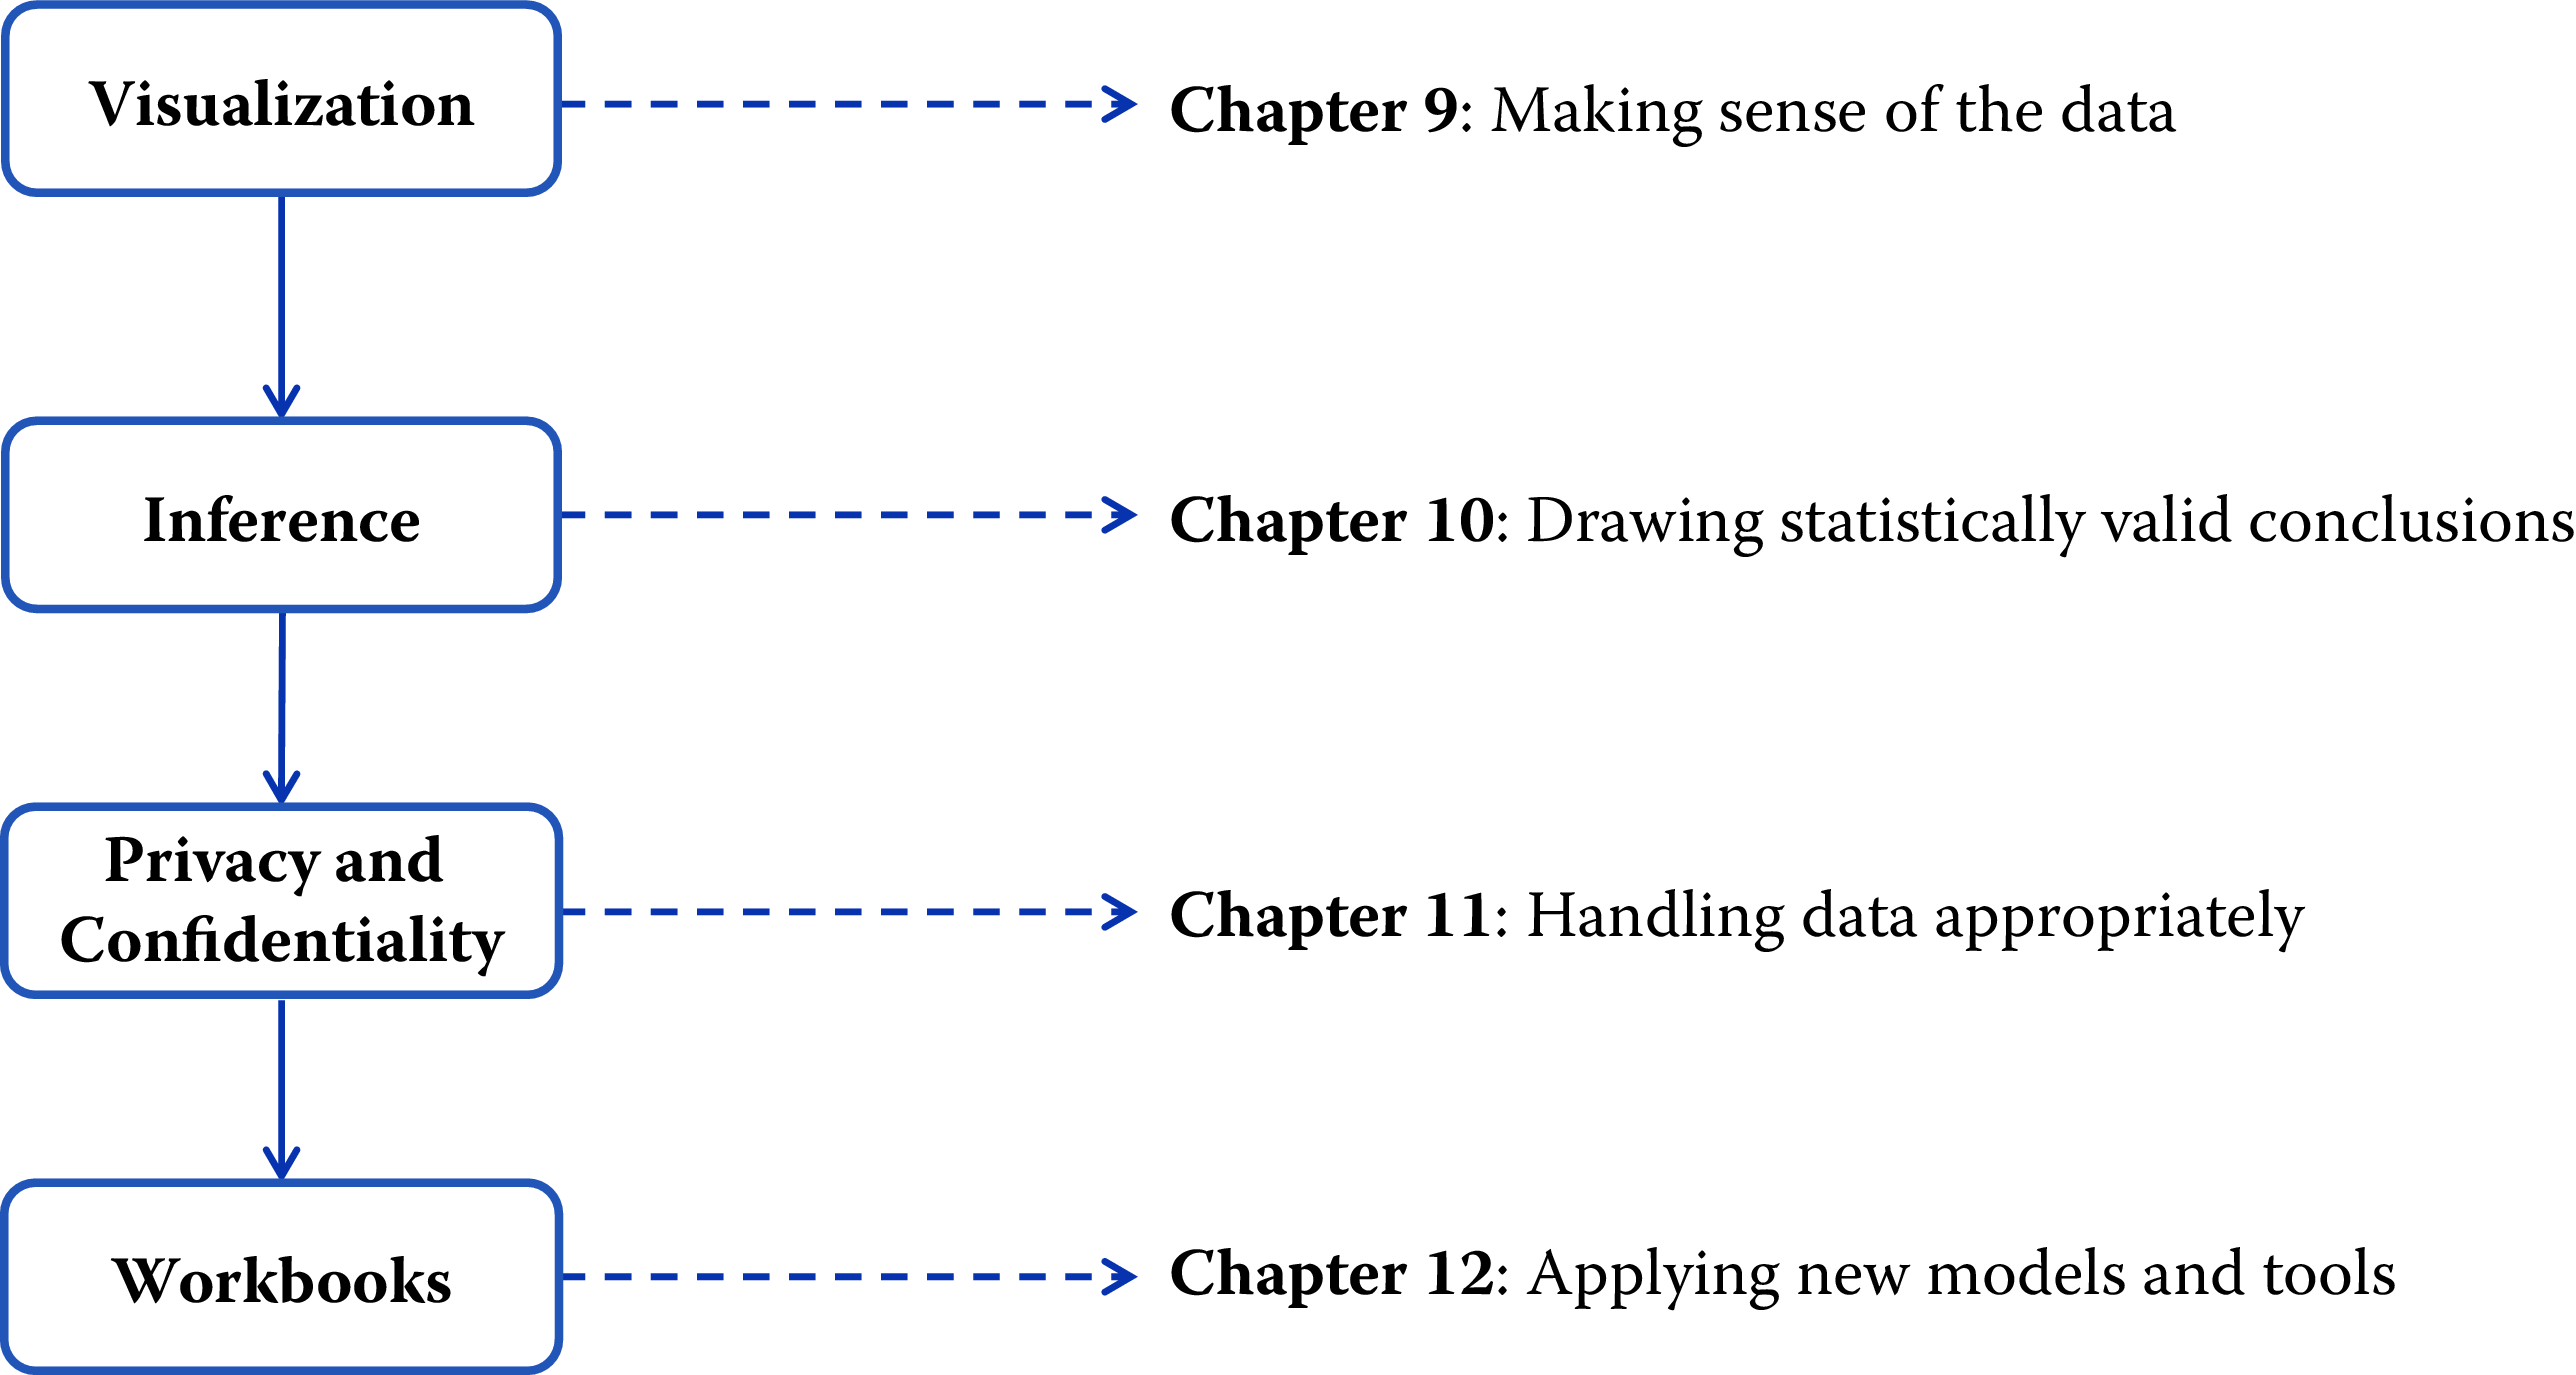
\includegraphics[width=0.7\linewidth]{ChapterIntro/figures/Figure4} 

}

\caption{The four chapters in Part III focus on *inference* and *ethics*}\label{fig:fig5}
\end{figure}

\hypertarget{sec:intro:resources}{\section{Resources}\label{sec:intro:resources}}

For more information on the \textbf{science of science policy}, see
Husbands et al.'s book for a full discussion of many issues (Husband
Fealing et al. \protect\hyperlink{ref-husband2011science}{2011}) and the
online resources at the eponymous website (SOSP, n.d.).

This book is above all a \emph{practical} introduction to the methods
and tools that the social scientist can use to make sense of big data,
and thus \textbf{programming} resources are also important. We make
extensive use of the Python programming language and the MySQL database
management system in both the book and its supporting workbooks. We
recommend that any social scientist who aspires to work with large data
sets become proficient in the use of these two systems, and also one
more, GitHub. All three, fortunately, are quite accessible and are
supported by excellent online resources. Time spent mastering them will
be repaid many times over in more productive research.

For \textbf{Python}\footnote{Read this!
  \url{http://alexbell.net/pyseminar/pyseminar.html}}, Alex Bell's
\emph{Python for Economists} (available online (Bell
\protect\hyperlink{ref-BellPython}{2012})) provides a wonderful 30-page
introduction to the use of Python in the social sciences, complete with
XKCD cartoons. Economists Tom Sargent and John Stachurski provide a very
useful set of lectures and examples at \url{http://quant-econ.net/}. For
more detail, we recommend Charles Severance's \emph{Python for
Informatics: Exploring Information} (Severance
\protect\hyperlink{ref-SeverancePython}{2013}), which not only covers
basic Python but also provides material relevant to web data (the
subject of \protect\hyperlink{chap:web}{Working with Web Data and APIs})
and MySQL (the subject of \protect\hyperlink{chap:db}{Databases}). This
book is also freely available online and is supported by excellent
online lectures and exercises.

For \textbf{MySQL}, Chapter \protect\hyperlink{chap:db}{Databases}
provides introductory material and pointers to additional resources, so
we will not say more here.

We also recommend that you master \textbf{GitHub}. A version control
system is a tool for keeping track of changes that have been made to a
document over time. GitHub is a hosting service for projects that use
the Git version control system. As Strasser explains (Strasser
\protect\hyperlink{ref-GitResearch}{2014}), Git/GitHub makes it
straightforward for researchers to create digital lab notebooks that
record the data files, programs, papers, and other resources associated
with a project, with automatic tracking of the changes that are made to
those resources over time. GitHub also makes it easy for collaborators
to work together on a project, whether a program or a paper: changes
made by each contributor are recorded and can easily be reconciled. For
example, we used GitHub to create this book, with authors and editors
checking in changes and comments at different times and from many time
zones. We also use GitHub to provide access to the supporting workbooks.
Ram (Ram \protect\hyperlink{ref-ram2013git}{2013}) provides a nice
description of how Git/GitHub can be used to promote reproducibility and
transparency in research.

One more resource that is outside the scope of this book but that you
may well want to master is the \textbf{cloud} (Armbrust et al.
\protect\hyperlink{ref-armbrust2010view}{2010}; Lifka et al.
\protect\hyperlink{ref-Lifka}{2013}). It used to be that when your data
and computations became too large to analyze on your laptop, you were
out of luck unless your employer (or a friend) had a larger computer.
With the emergence of cloud storage and computing services from the
likes of Amazon Web Services, Google, and Microsoft, powerful computers
are available to anyone with a credit card. We and many others have had
positive experiences using such systems for the analysis of urban
(Catlett et al. \protect\hyperlink{ref-plenario}{2014}), environmental
(Elliott et al. \protect\hyperlink{ref-elliott2014parallel}{2014}), and
genomic (Bhuvaneshwar et al.
\protect\hyperlink{ref-bhuvaneshwar2015case}{2015}) data analysis and
modeling, for example. Such systems may well represent the future of
research computing.

\hypertarget{chap:web}{\chapter{Working with Web Data and
APIs}\label{chap:web}}

\textbf{Cameron Neylon}

In many social science problems we have to augment our data with
external data sources. Often the data we use for augmenting are
available on the web, either on web pages directly or accessible through
Application Programming Interfaces (APIs). Gathering this data requires
understanding how to scrape web pages or calling the APIs with
parameters about the information we need. For example, we often augment
our primary data with data from the American Community Survey (ACS) or
from Open Data Portals being maintained by local, state, and federal
agencies. These data sources can either be downloaded in bulk or used
``on-demand'' through APIs. Same is true for data from social media
sources, such as Twitter, and Facebook. In this chapter we will cover
tools that can be used by social science researchers to gather this type
of external data from web pages and APIs.

\section{Introduction}\label{introduction}

A tremendous lure of the Internet is the availability of vast amounts of
data on businesses, people, and their activity on social media. But how
can we capture the information and make use of it as we might make use
of more traditional data sources?

In social science, we are often exploring information on people or on a
group of people. The web can be a rich source of additional information.
It can also act as pointers to new sources of information, allowing a
pivot from one perspective to another, from one kind of query to
another. Often this is exploratory. You have an existing core set of
data and are looking to augment it. But equally this exploration can
open up whole new avenues. Sometimes the data are completely
unstructured, existing as web pages spread across a site, and sometimes
they are provided in a machine-readable form. The challenge is in having
a sufficiently diverse toolkit to bring all of this information
together.

Using the example of data on researchers and research outputs, we will
Focus this chapter on obtaining information directly from web pages
(\emph{web scraping}) as well as explore the uses of APIs--- web
services that allow an interaction with, and retrieval of data. You will
see how the crucial pieces of integration often lie in making
connections between disparate data sets and how in turn making those
connections requires careful quality control. The emphasis throughout
this chapter is on the importance of focusing on the purpose for which
the data will be used as a guide for data collection. While much of this
is specific to data about research and researchers, the ideas are
generalizable to wider issues of data and public policy.

\section{Scraping information from the web}\label{sec:4-1}

With the range of information available on the web, our first question
is how to access it. The simplest approach is often to manually go
directly to the web and look for data files or other information. For
instance, on the NSF website (National Science Foundation, n.d.) it is
possible to obtain data dumps of all grant information. Sometimes data
are available through web pages or we only want a subset of this
information. In this case web scraping is often a viable approach.

Web scraping involves writing code to download and process web pages
directly. We need to look at the website, identify how to get the
information we want, and then process it. Many websites deliberately
make this difficult to prevent easy access to their underlying data.

\subsection{Obtaining data from websites}\label{sec:4-1.1}

Let us suppose we are interested in obtaining information on those
investigators that are funded by the Howard Hughes Medical Institute
(HHMI). HHMI has a website that includes a search function for funded
researchers, including the ability to filter by field, state, and role.
But there does not appear to be a downloadable data set of this
information. However, we can automate the process with code to create a
data set that you might compare with other data.

\url{https://www.hhmi.org/scientists/browse?sort_by=field_scientist_last_name\&sort_order=ASC\&items_per_page=24}

Getting information from this web page programmatically requires us to
follow the following steps: Constructing a URL that will give us the
results we want Fetching the page using that URL Processing the html
response to extract the pieces of information we are lookin for (such as
names and specialties of the scientists)

Constructing the URL This process involves first understanding how to
construct a URL that will do the search we want. This is most easily
done by playing with search functionality and investigating the URL
structures that are returned.

With HHMI, if we do a general search and play with the structure of the
URL, we can see some of the elements of the URL that we can think of as
a query. As we want to see \emph{all} investigators, we do not need to
limit the search, and so with some fiddling we come up with a URL like
the following. (We have broken the one-line URL into three lines for
ease of presentation.)

\enlargethispage{6pt}

\url{http://www.hhmi.org/scientists/browse?kw}=\&sort\_by=field\_scientist\_last\_name\&sort\_order=ASC\&items\_per\_page=24\&page=0

We can click on different links on the page modify part of this URL to
see how the search results change. For example, if we click on Sort by
Institution, the URL changes to

\url{https://www.hhmi.org/scientists/browse?sort_by=field_scientist_academic_institu\&sort_order=ASC\&items_per_page=24\&page=0}

If we click on next at the bottom, the url changes to
\url{https://www.hhmi.org/scientists/browse?sort_by=field_scientist_academic_institu\&sort_order=ASC\&items_per_page=24\&page=1}

This allows us to see that the URL is constructed using a few
parameters, such as sort\_by, sort\_order, items\_per\_page, and page
that can be programmatically modified to give us the search results that
we want.

\textbf{Getting the contents of the page from the URL}

The \texttt{requests} module, available natively in Jupyter Python
notebooks, is a useful set of tools for handling interactions with
websites. It lets us construct the request that we just presented in
terms of a base URL and query terms, as follows:

\begin{Shaded}
\begin{Highlighting}[]
\OperatorTok{>}\ErrorTok{>}\StringTok{ }\NormalTok{BASE_URL =}\StringTok{ "http://www.hhmi.org/scientists/browse"}
\OperatorTok{>}\ErrorTok{>}\StringTok{ }\NormalTok{query =}\StringTok{ }\NormalTok{\{}
            \StringTok{"kw"} \OperatorTok{:}\StringTok{ ""}\NormalTok{,}
            \StringTok{"sort_by"} \OperatorTok{:}\StringTok{ "field_scientist_last_name"}\NormalTok{,}
            \StringTok{"sort_order"} \OperatorTok{:}\StringTok{ "ASC"}\NormalTok{,}
            \StringTok{"items_per_page"} \OperatorTok{:}\StringTok{ }\DecValTok{24}\NormalTok{,}
            \StringTok{"page"} \OperatorTok{:}\StringTok{ }\NormalTok{None}
\NormalTok{           \}}
\end{Highlighting}
\end{Shaded}

With our request constructed we can then make the call to the web page
to get a response.

\begin{Shaded}
\begin{Highlighting}[]
\OperatorTok{>}\ErrorTok{>}\StringTok{ }\NormalTok{import requests}
\OperatorTok{>}\ErrorTok{>}\StringTok{ }\NormalTok{response =}\StringTok{ }\KeywordTok{requests.get}\NormalTok{(BASE_URL, }\DataTypeTok{params=}\NormalTok{query)}
\end{Highlighting}
\end{Shaded}

The first thing to do when building a script that hits a web page is to
make sure that your call was successful. This can be checked by looking
at the response code that the web server sent---and, obviously, by
checking the actual HTML that was returned. A \texttt{200} code means
success and that everything should be OK. Other codes may mean that the
URL was constructed wrongly or that there was a server error.

\begin{Shaded}
\begin{Highlighting}[]
\OperatorTok{>}\ErrorTok{>}\StringTok{ }\NormalTok{response.status_code}
\DecValTok{200}
\end{Highlighting}
\end{Shaded}

\textbf{Processing the html response}

With the page successfully returned, we now need to process the text it
contains into the data we want. This is not a trivial exercise. It is
possible to search through and find things, but there are a range of
tools that can help with processing HTML and XML data. Among these one
of the most popular is a module called BeautifulSoup\footnote{Python
  features many useful libraries; BeautifulSoup is particularly helpful
  for webscraping.} (Richardson, n.d.), which provides a number of
useful functions for this kind of processing. The module documentation
provides more details.

We need to check the details of the page source to find where the
information we are looking for is kept (see, for example,
\ref{fig:fig2-1}). Here, all the details on HHMI investigators can be
found in a \texttt{\textless{}div\textgreater{}} element with the class
attribute \texttt{view-content}. This structure is not something that
can be determined in advance. It requires knowledge of the structure of
the page itself. Nested inside this
\texttt{\textless{}div\textgreater{}} element are another series of
\texttt{div}s, each of which corresponds to one investigator. These have
the class attribute \texttt{view-rows}. Again, there is nothing obvious
about finding these, it requires a close examination of the page HTML
itself for any specific case you happen to be looking at.

\begin{figure}

{\centering 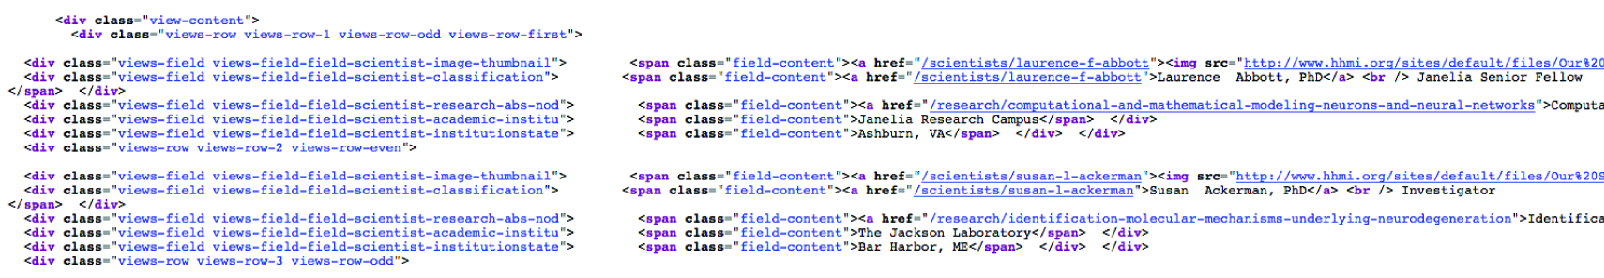
\includegraphics[width=0.7\linewidth]{ChapterWeb/figures/fig2-1} 

}

\caption{Source HTML from the portion of an HHMI results page containing information on HHMI investigators; note that the webscraping results in badly formatted html which is difficult to read.}\label{fig:fig2-1}
\end{figure}

\vspace*{-8pt} We first process the page using the BeautifulSoup module
(into the variable \texttt{soup}) and then find the \texttt{div} element
that holds the information on investigators
(\texttt{investigator\_list}). As this element is unique on the page (I
checked using my web browser), we can use the find method. We then
process that \texttt{div} (using \texttt{find\_all}) to create an
iterator object that contains each of the page segments detailing a
single investigator (\texttt{investigators}).

\begin{Shaded}
\begin{Highlighting}[]
\OperatorTok{>}\ErrorTok{>}\StringTok{ }\NormalTok{from bs4 import BeautifulSoup}
\OperatorTok{>}\ErrorTok{>}\StringTok{ }\NormalTok{soup =}\StringTok{ }\KeywordTok{BeautifulSoup}\NormalTok{(response.text, }\StringTok{"html5lib"}\NormalTok{)}
\OperatorTok{>}\ErrorTok{>}\StringTok{ }\NormalTok{investigator_list =}\StringTok{ }\KeywordTok{soup.find}\NormalTok{(}\StringTok{'div'}\NormalTok{, }\DataTypeTok{class_ =} \StringTok{"view-content"}\NormalTok{)}
\OperatorTok{>}\ErrorTok{>}\StringTok{ }\NormalTok{investigators =}\StringTok{ }\KeywordTok{investigator_list.find_all}\NormalTok{(}\StringTok{"div"}\NormalTok{, }\DataTypeTok{class_ =} \StringTok{"views-row"}\NormalTok{)}
\end{Highlighting}
\end{Shaded}

\enlargethispage{24pt} As we specified in our query parameters that we
wanted 24 results per page, we should check whether our list of page
sections has the right length.

\begin{Shaded}
\begin{Highlighting}[]
\OperatorTok{>}\ErrorTok{>}\StringTok{ }\KeywordTok{len}\NormalTok{(investigators)}
\DecValTok{20}
\end{Highlighting}
\end{Shaded}

\enlargethispage{12pt}

\begin{Shaded}
\begin{Highlighting}[]
\CommentTok{# Given a request response object, parse for HHMI investigators}
\NormalTok{def }\KeywordTok{scrape}\NormalTok{(page_response)}\OperatorTok{:}
\StringTok{   }\CommentTok{# Obtain response HTML and the correct <div> from the page}
\StringTok{   }\NormalTok{soup =}\StringTok{ }\KeywordTok{BeautifulSoup}\NormalTok{(response.text, }\StringTok{"html5lib"}\NormalTok{)}
\NormalTok{   inv_list =}\StringTok{ }\KeywordTok{soup.find}\NormalTok{(}\StringTok{'div'}\NormalTok{, }\DataTypeTok{class_ =} \StringTok{"view-content"}\NormalTok{)}

   \CommentTok{# Create a list of all the investigators on the page}
\NormalTok{   investigators =}\StringTok{ }\KeywordTok{inv_list.find_all}\NormalTok{(}\StringTok{"div"}\NormalTok{, }\DataTypeTok{class_ =} \StringTok{"views-row"}\NormalTok{)}

\NormalTok{   data =}\StringTok{ }\NormalTok{[] }\CommentTok{# Make the data object to store scraping results}

   \CommentTok{# Scrape needed elements from investigator list}
   \ControlFlowTok{for}\NormalTok{ investigator }\ControlFlowTok{in}\NormalTok{ investigators}\OperatorTok{:}
\StringTok{       }\NormalTok{inv =}\StringTok{ }\NormalTok{\{\} }\CommentTok{# Create a dictionary to store results}

       \CommentTok{# Name and role are in same HTML element; this code}
       \CommentTok{# separates them into two data elements}
\NormalTok{       name_role_tag =}\StringTok{ }\KeywordTok{investigator.find}\NormalTok{(}\StringTok{"div"}\NormalTok{,}
           \DataTypeTok{class_ =} \StringTok{"views-field-field-scientist-classification"}\NormalTok{)}
\NormalTok{       strings =}\StringTok{ }\NormalTok{name_role_tag.stripped_strings}
       \ControlFlowTok{for}\NormalTok{ string,a }\ControlFlowTok{in} \KeywordTok{zip}\NormalTok{(strings, [}\StringTok{"name"}\NormalTok{, }\StringTok{"role"}\NormalTok{])}\OperatorTok{:}
\StringTok{           }\NormalTok{inv[a] =}\StringTok{ }\NormalTok{string}

       \CommentTok{# Extract other elements from text of specific divs or from}
       \CommentTok{# class attributes of tags in the page (e.g., URLs)}
\NormalTok{       research_tag =}\StringTok{ }\KeywordTok{investigator.find}\NormalTok{(}\StringTok{"div"}\NormalTok{,}
          \DataTypeTok{class_ =} \StringTok{"views-field-field-scientist-research-abs-nod"}\NormalTok{)}
\NormalTok{       inv[}\StringTok{"research"}\NormalTok{] =}\StringTok{ }\KeywordTok{research_tag.text.lstrip}\NormalTok{()}
\NormalTok{       inv[}\StringTok{"research_url"}\NormalTok{] =}\StringTok{ "http://hhmi.org"}
          \OperatorTok{+}\StringTok{ }\KeywordTok{research_tag.find}\NormalTok{(}\StringTok{"a"}\NormalTok{)}\KeywordTok{.get}\NormalTok{(}\StringTok{"href"}\NormalTok{)}
\NormalTok{       institution_tag =}\StringTok{ }\KeywordTok{investigator.find}\NormalTok{(}\StringTok{"div"}\NormalTok{,}
          \DataTypeTok{class_ =} \StringTok{"views-field-field-scientist-academic-institu"}\NormalTok{)}
\NormalTok{       inv[}\StringTok{"institute"}\NormalTok{] =}\StringTok{ }\KeywordTok{institution_tag.text.lstrip}\NormalTok{()}
\NormalTok{       town_state_tag =}\StringTok{ }\KeywordTok{investigator.find}\NormalTok{(}\StringTok{"div"}\NormalTok{,}
           \DataTypeTok{class_ =} \StringTok{"views-field-field-scientist-institutionstate"}\NormalTok{)}
\NormalTok{       inv[}\StringTok{"town"}\NormalTok{], inv[}\StringTok{"state"}\NormalTok{] =}\StringTok{ }\KeywordTok{town_state_tag.text.split}\NormalTok{(}\StringTok{","}\NormalTok{)}
\NormalTok{       inv[}\StringTok{"town"}\NormalTok{] =}\StringTok{ }\KeywordTok{inv.get}\NormalTok{(}\StringTok{"town"}\NormalTok{)}\KeywordTok{.lstrip}\NormalTok{()}
\NormalTok{       inv[}\StringTok{"state"}\NormalTok{] =}\StringTok{ }\KeywordTok{inv.get}\NormalTok{(}\StringTok{"state"}\NormalTok{)}\KeywordTok{.lstrip}\NormalTok{()}

\NormalTok{       thumbnail_tag =}\StringTok{ }\KeywordTok{investigator.find}\NormalTok{(}\StringTok{"div"}\NormalTok{,}
          \DataTypeTok{class_ =} \StringTok{"views-field-field-scientist-image-thumbnail"}\NormalTok{)}
\NormalTok{       inv[}\StringTok{"thumbnail_url"}\NormalTok{] =}\StringTok{ }\KeywordTok{thumbnail_tag.find}\NormalTok{(}\StringTok{"img"}\NormalTok{)[}\StringTok{"src"}\NormalTok{]}
\NormalTok{       inv[}\StringTok{"url"}\NormalTok{] =}\StringTok{ "http://hhmi.org"}
          \OperatorTok{+}\StringTok{ }\KeywordTok{thumbnail_tag.find}\NormalTok{(}\StringTok{"a"}\NormalTok{)}\KeywordTok{.get}\NormalTok{(}\StringTok{"href"}\NormalTok{)}

       \CommentTok{# Add the new data to the list}
       \KeywordTok{data.append}\NormalTok{(inv)}
\NormalTok{   return data}
\end{Highlighting}
\end{Shaded}

Listing 2.1. Python code to parse for HHMI investigators

\pagebreak
Finally, we need to process each of these segments to obtain the data we
are looking for. This is the actual ``scraping'' of the page to get the
information we want. Again, this involves looking closely at the HTML
itself, identifying where the information is held, what tags can be used
to find it, and often doing some postprocessing to clean it up (removing
spaces, splitting different elements up).

Listing 2.1 provides a function to handle all of this. The function
accepts the response object from the requests module as its input,
processes the page text to soup, and then finds the
\texttt{investigator\_list} as above and processes it into an actual
list of the investigators. For each investigator it then processes the
HTML to find and clean up the information required, converting it to a
dictionary and adding it to our growing list of data.

Let us check what the first two elements of our data set now look like.
You can see two dictionaries, one relating to Laurence Abbott, who is a
senior fellow at the HHMI Janelia Farm Campus, and one for Susan
Ackerman, an HHMI investigator based at the Jackson Laboratory in Bar
Harbor, Maine. Note that we have also obtained URLs that give more
details on the researcher and their research program
(\texttt{research\_url} and \texttt{url} keys in the dictionary) that
could provide a useful input to textual analysis or topic modeling (see
\protect\hyperlink{chap:text}{Text Analysis}).

\begin{Shaded}
\begin{Highlighting}[]
\OperatorTok{>}\ErrorTok{>}\StringTok{ }\NormalTok{data =}\StringTok{ }\KeywordTok{scrape}\NormalTok{(response)}
\OperatorTok{>}\ErrorTok{>}\StringTok{ }\NormalTok{data[}\DecValTok{0}\OperatorTok{:}\DecValTok{2}\NormalTok{]}
\NormalTok{[\{}\StringTok{'institute'}\OperatorTok{:}\StringTok{ }\NormalTok{u}\StringTok{'Janelia Research Campus '}\NormalTok{,}
  \StringTok{'name'}\OperatorTok{:}\StringTok{ }\NormalTok{u}\StringTok{'Laurence Abbott, PhD'}\NormalTok{,}
  \StringTok{'research'}\OperatorTok{:}\StringTok{ }\NormalTok{u}\StringTok{'Computational and Mathematical Modeling of Neurons and Neural... '}\NormalTok{,}
  \StringTok{'research_url'}\OperatorTok{:}\StringTok{ }\NormalTok{u}\StringTok{'http://hhmi.org/research/computational-and-mathematical-modeling-neurons-and-neural-networks'}\NormalTok{,}
  \StringTok{'role'}\OperatorTok{:}\StringTok{ }\NormalTok{u}\StringTok{'Janelia Senior Fellow'}\NormalTok{,}
  \StringTok{'state'}\OperatorTok{:}\StringTok{ }\NormalTok{u}\StringTok{'VA '}\NormalTok{,}
  \StringTok{'thumbnail_url'}\OperatorTok{:}\StringTok{ }\NormalTok{u}\StringTok{'http://www.hhmi.org/sites/default/files/Our%20Scientists/Janelia/Abbott-112x112.jpg'}\NormalTok{,}
  \StringTok{'town'}\OperatorTok{:}\StringTok{ }\NormalTok{u}\StringTok{'Ashburn'}\NormalTok{,}
  \StringTok{'url'}\OperatorTok{:}\StringTok{ }\NormalTok{u}\StringTok{'http://hhmi.org/scientists/laurence-f-abbott'}\NormalTok{\},}
\NormalTok{ \{}\StringTok{'institute'}\OperatorTok{:}\StringTok{ }\NormalTok{u}\StringTok{'The Jackson Laboratory '}\NormalTok{,}
  \StringTok{'name'}\OperatorTok{:}\StringTok{ }\NormalTok{u}\StringTok{'Susan Ackerman, PhD'}\NormalTok{,}
  \StringTok{'research'}\OperatorTok{:}\StringTok{ }\NormalTok{u}\StringTok{'Identification of the Molecular Mechanisms Underlying... '}\NormalTok{,}
  \StringTok{'research_url'}\OperatorTok{:}\StringTok{ }\NormalTok{u}\StringTok{'http://hhmi.org/research/identification-molecular-mechanisms-underlying-neurodegeneration'}\NormalTok{,}
  \StringTok{'role'}\OperatorTok{:}\StringTok{ }\NormalTok{u}\StringTok{'Investigator'}\NormalTok{,}
  \StringTok{'state'}\OperatorTok{:}\StringTok{ }\NormalTok{u}\StringTok{'ME '}\NormalTok{,}
  \StringTok{'thumbnail_url'}\OperatorTok{:}
\NormalTok{u}\StringTok{'http://www.hhmi.org/sites/default/files/Our%20Scientists/Investigators/Ackerman-112x112.jpg'}\NormalTok{,}
  \StringTok{'town'}\OperatorTok{:}\StringTok{ }\NormalTok{u}\StringTok{'Bar Harbor'}\NormalTok{,}
  \StringTok{'url'}\OperatorTok{:}\StringTok{ }\NormalTok{u}\StringTok{'http://hhmi.org/scientists/susan-l-ackerman'}\NormalTok{\}]}
\end{Highlighting}
\end{Shaded}

Programmatically Iterating over the Search Results

So now we know we can process a page from a website to generate usefully
structured data. However, this was only the first page of results. We
need to do this for each page of results if we want to capture all the
HHMI investigators. We could just look at the number of pages that our
search returned manually, but to make this more general we can actually
scrape the page to find that piece of information and use that to
calculate how many pages we need to work through.

The number of results is found in a \texttt{div} with the class
``view-headers'' as a piece of free text (``Showing 1--20 of 493
results''). We need to grab the text, split it up (I do so based on
spaces), find the right number (the one that is before the word
``results'') and convert that to an integer. Then we can divide by the
number of items we requested per page (20 in our case) to find how many
pages we need to work through. A quick mental calculation confirms that
if page 0 had results 1--20, page 24 would give results 481--493.

\begin{Shaded}
\begin{Highlighting}[]
\OperatorTok{>}\ErrorTok{>}\StringTok{ }\CommentTok{# Check total number of investigators returned}
\ErrorTok{>>}\StringTok{ }\NormalTok{view_header =}\StringTok{ }\KeywordTok{soup.find}\NormalTok{(}\StringTok{"div"}\NormalTok{, }\DataTypeTok{class_ =} \StringTok{"view-header"}\NormalTok{)}
\OperatorTok{>}\ErrorTok{>}\StringTok{ }\NormalTok{words =}\StringTok{ }\KeywordTok{view_header.text.split}\NormalTok{(}\StringTok{" "}\NormalTok{)}
\OperatorTok{>}\ErrorTok{>}\StringTok{ }\NormalTok{count_index =}\StringTok{ }\KeywordTok{words.index}\NormalTok{(}\StringTok{"results."}\NormalTok{) }\OperatorTok{-}\StringTok{ }\DecValTok{1}
\OperatorTok{>}\ErrorTok{>}\StringTok{ }\NormalTok{count =}\StringTok{ }\KeywordTok{int}\NormalTok{(words[count_index])}

\OperatorTok{>}\ErrorTok{>}\StringTok{ }\CommentTok{# Calculate number of pages, given count & items_per_page}
\ErrorTok{>>}\StringTok{ }\NormalTok{num_pages =}\StringTok{ }\NormalTok{count}\OperatorTok{/}\KeywordTok{query.get}\NormalTok{(}\StringTok{"items_per_page"}\NormalTok{)}
\OperatorTok{>}\ErrorTok{>}\StringTok{ }\NormalTok{num_pages}
\DecValTok{24}
\end{Highlighting}
\end{Shaded}

Then it is a simple matter of putting the function we constructed
earlier into a loop to work through the correct number of pages. As we
start to hit the website repeatedly, we need to consider whether we are
being polite. Most websites have a file in the root directory called
robots.txt that contains guidance on using programs to interact with the
website. In the case of \url{http://hhmi.org} the file states first that
we are allowed (or, more properly, not forbidden) to query
\url{http://www.hhmi.org/scientists/} programmatically. Thus, you can
pull down all of the more detailed biographical or research information,
if you so desire. The file also states that there is a requested
``Crawl-delay'' of 10. This means that if you are making repeated
queries (as we will be in getting the 24 pages), you should wait for 10
seconds between each query. This request is easily accommodated by
adding a timed delay between each page request.

\pagebreak

\begin{Shaded}
\begin{Highlighting}[]
\OperatorTok{>}\ErrorTok{>}\StringTok{ }\ControlFlowTok{for}\NormalTok{ page_num }\ControlFlowTok{in} \KeywordTok{range}\NormalTok{(num_pages)}\OperatorTok{:}
\ErrorTok{>>}\StringTok{ }\CommentTok{# We already have page zero and we need to go to 24:}
\ErrorTok{>>}\StringTok{ }\CommentTok{# range(24) is [0,1,...,23]}
\ErrorTok{>>}\StringTok{    }\NormalTok{query[}\StringTok{"items_per_page"}\NormalTok{] =}\StringTok{ }\NormalTok{page_num }\OperatorTok{+}\StringTok{ }\DecValTok{1}
\OperatorTok{>}\ErrorTok{>}\StringTok{    }\NormalTok{page =}\StringTok{ }\KeywordTok{requests.get}\NormalTok{(BASE_URL, }\DataTypeTok{params=}\NormalTok{query)}
\OperatorTok{>}\ErrorTok{>}\StringTok{ }\CommentTok{# We use extend to add list for each page to existing list}
\ErrorTok{>>}\StringTok{    }\KeywordTok{data.extend}\NormalTok{(}\KeywordTok{scrape}\NormalTok{(page))}
\OperatorTok{>}\ErrorTok{>}\StringTok{ }\KeywordTok{print}\NormalTok{(}\StringTok{"Retrieved and scraped page number:"}\NormalTok{, }\KeywordTok{query.get}\NormalTok{(}\StringTok{"items_per_page"}\NormalTok{))}
\OperatorTok{>}\ErrorTok{>}\StringTok{ }\KeywordTok{time.sleep}\NormalTok{(}\DecValTok{10}\NormalTok{) }\CommentTok{# robots.txt at hhmi.org specifies a crawl delay of 10 seconds}
\NormalTok{Retrieved and scraped page number}\OperatorTok{:}\StringTok{ }\DecValTok{1}
\NormalTok{Retrieved and scraped page number}\OperatorTok{:}\StringTok{ }\DecValTok{2}
\NormalTok{...}
\NormalTok{Retrieved and scraped page number}\OperatorTok{:}\StringTok{ }\DecValTok{24}
\end{Highlighting}
\end{Shaded}

Finally we can check that we have the right number of results after our
scraping. This should correspond to the 493 records that the website
reports.

\begin{Shaded}
\begin{Highlighting}[]
\OperatorTok{>}\ErrorTok{>}\StringTok{ }\KeywordTok{len}\NormalTok{(data)}
\DecValTok{493}
\end{Highlighting}
\end{Shaded}

\subsection{Limits of scraping}\label{sec:4-1.2}

While scraping websites is often necessary, is can be a fragile and
messy way of working. It is problematic for a number of reasons: for
example, many websites are designed in ways that make scraping difficult
or impossible, and other sites explicitly prohibit this kind of scripted
analysis. (Both reasons apply in the case of the NSF and Grants.gov
websites, which is why we use the HHMI website in our example.) The
structure of websites also changes frequently, forcing you to
continuously modify your code to match the structure.

In many cases a better choice is to process a data dump from an
organization. For example, the NSF and Wellcome Trust both provide data
sets for each year that include structured data on all their awarded
grants. In practice, integrating data is a continual challenge of
figuring out what is the easiest way to proceed, what is allowed, and
what is practical and useful. The selection of data will often be driven
by pragmatic rather than theoretical concerns.

Increasingly, however, good practice is emerging in which organizations
provide APIs to enable scripted and programmatic access to the data they
hold. These tools are much easier and generally more effective to work
with. They are the focus of much of the rest of this chapter.

\begin{center}\rule{0.5\linewidth}{\linethickness}\end{center}

\section{Application Programming Interfaces (APIs)}\label{sec:4-3}

An API is simply a tool that allows a program to interface with a
service. APIs can take many different forms and be of varying quality
and usefulness. In this section we will focus on one common type of API
and examples of important publicly available APIs relevant to research
communications. We will also cover combining APIs and the benefits and
challenges of bringing multiple data sources together.

\subsection{Relevant APIs and resources}\label{sec:4-3.1}

There is a wide range of other sources of information that can be used
in combination with the APIs featured above to develop an overview of
research outputs and of where and how they are being used. There are
also other tools that can allow deeper analysis of the outputs
themselves. Table \ref{tab:table2-1} gives a partial list of key data
sources and APIs that are relevant to the analysis of research outputs.

\begin{longtable}[]{@{}llcc@{}}
\caption{\label{tab:table2-1} Popular sources of data relevant to the
analysis of research outputs}\tabularnewline
\toprule
\begin{minipage}[b]{0.10\columnwidth}\raggedright\strut
\textbf{Source}\strut
\end{minipage} & \begin{minipage}[b]{0.74\columnwidth}\raggedright\strut
\textbf{Description}\strut
\end{minipage} & \begin{minipage}[b]{0.02\columnwidth}\centering\strut
\textbf{API}\strut
\end{minipage} & \begin{minipage}[b]{0.02\columnwidth}\centering\strut
\textbf{Free}\strut
\end{minipage}\tabularnewline
\midrule
\endfirsthead
\toprule
\begin{minipage}[b]{0.10\columnwidth}\raggedright\strut
\textbf{Source}\strut
\end{minipage} & \begin{minipage}[b]{0.74\columnwidth}\raggedright\strut
\textbf{Description}\strut
\end{minipage} & \begin{minipage}[b]{0.02\columnwidth}\centering\strut
\textbf{API}\strut
\end{minipage} & \begin{minipage}[b]{0.02\columnwidth}\centering\strut
\textbf{Free}\strut
\end{minipage}\tabularnewline
\midrule
\endhead
\begin{minipage}[t]{0.10\columnwidth}\raggedright\strut
\strut
\end{minipage} & \begin{minipage}[t]{0.74\columnwidth}\raggedright\strut
\textbf{Bibliographic Data}\strut
\end{minipage} & \begin{minipage}[t]{0.02\columnwidth}\centering\strut
\strut
\end{minipage} & \begin{minipage}[t]{0.02\columnwidth}\centering\strut
\strut
\end{minipage}\tabularnewline
\begin{minipage}[t]{0.10\columnwidth}\raggedright\strut
PubMed\strut
\end{minipage} & \begin{minipage}[t]{0.74\columnwidth}\raggedright\strut
An online index that combines bibliographic data from Medline and PubMed
Central. PubMed Central and Europe PubMed Central also provide
information.\strut
\end{minipage} & \begin{minipage}[t]{0.02\columnwidth}\centering\strut
Y\strut
\end{minipage} & \begin{minipage}[t]{0.02\columnwidth}\centering\strut
Y\strut
\end{minipage}\tabularnewline
\begin{minipage}[t]{0.10\columnwidth}\raggedright\strut
Web of Science\strut
\end{minipage} & \begin{minipage}[t]{0.74\columnwidth}\raggedright\strut
The bibliographic database provided by Thomson Reuters. The ISI Citation
Index is also available.\strut
\end{minipage} & \begin{minipage}[t]{0.02\columnwidth}\centering\strut
Y\strut
\end{minipage} & \begin{minipage}[t]{0.02\columnwidth}\centering\strut
N\strut
\end{minipage}\tabularnewline
\begin{minipage}[t]{0.10\columnwidth}\raggedright\strut
Scopus\strut
\end{minipage} & \begin{minipage}[t]{0.74\columnwidth}\raggedright\strut
The bibliographic database provided by Elsevier. It also provides
citation information.\strut
\end{minipage} & \begin{minipage}[t]{0.02\columnwidth}\centering\strut
Y\strut
\end{minipage} & \begin{minipage}[t]{0.02\columnwidth}\centering\strut
N\strut
\end{minipage}\tabularnewline
\begin{minipage}[t]{0.10\columnwidth}\raggedright\strut
Crossref\strut
\end{minipage} & \begin{minipage}[t]{0.74\columnwidth}\raggedright\strut
Provides a range of bibliographic metadata and information obtained from
members registering DOIs.\strut
\end{minipage} & \begin{minipage}[t]{0.02\columnwidth}\centering\strut
Y\strut
\end{minipage} & \begin{minipage}[t]{0.02\columnwidth}\centering\strut
Y\strut
\end{minipage}\tabularnewline
\begin{minipage}[t]{0.10\columnwidth}\raggedright\strut
Google Scholar\strut
\end{minipage} & \begin{minipage}[t]{0.74\columnwidth}\raggedright\strut
Provides a search index for scholarly objects and aggregates citation
information.\strut
\end{minipage} & \begin{minipage}[t]{0.02\columnwidth}\centering\strut
N\strut
\end{minipage} & \begin{minipage}[t]{0.02\columnwidth}\centering\strut
Y\strut
\end{minipage}\tabularnewline
\begin{minipage}[t]{0.10\columnwidth}\raggedright\strut
Microsoft Academic Search\strut
\end{minipage} & \begin{minipage}[t]{0.74\columnwidth}\raggedright\strut
Provides a search index for scholarly objects and aggregates citation
information. Not as complete as Google Scholar, but has an API.\strut
\end{minipage} & \begin{minipage}[t]{0.02\columnwidth}\centering\strut
Y\strut
\end{minipage} & \begin{minipage}[t]{0.02\columnwidth}\centering\strut
Y\strut
\end{minipage}\tabularnewline
\begin{minipage}[t]{0.10\columnwidth}\raggedright\strut
\strut
\end{minipage} & \begin{minipage}[t]{0.74\columnwidth}\raggedright\strut
\textbf{Social Media}\strut
\end{minipage} & \begin{minipage}[t]{0.02\columnwidth}\centering\strut
\strut
\end{minipage} & \begin{minipage}[t]{0.02\columnwidth}\centering\strut
\strut
\end{minipage}\tabularnewline
\begin{minipage}[t]{0.10\columnwidth}\raggedright\strut
Altmetric.com\strut
\end{minipage} & \begin{minipage}[t]{0.74\columnwidth}\raggedright\strut
A provider of aggregated data on social media and mainstream media
attention of research outputs. Most comprehensive source of information
across different social media and mainstream media conversations.\strut
\end{minipage} & \begin{minipage}[t]{0.02\columnwidth}\centering\strut
Y\strut
\end{minipage} & \begin{minipage}[t]{0.02\columnwidth}\centering\strut
N\strut
\end{minipage}\tabularnewline
\begin{minipage}[t]{0.10\columnwidth}\raggedright\strut
Twitter\strut
\end{minipage} & \begin{minipage}[t]{0.74\columnwidth}\raggedright\strut
Provides an API that allows a user to search for recent tweets and
obtain some information on specific accounts.\strut
\end{minipage} & \begin{minipage}[t]{0.02\columnwidth}\centering\strut
Y\strut
\end{minipage} & \begin{minipage}[t]{0.02\columnwidth}\centering\strut
Y\strut
\end{minipage}\tabularnewline
\begin{minipage}[t]{0.10\columnwidth}\raggedright\strut
Facebook\strut
\end{minipage} & \begin{minipage}[t]{0.74\columnwidth}\raggedright\strut
The Facebook API gives information on the number of pages, likes, and
posts associated with specific web pages\strut
\end{minipage} & \begin{minipage}[t]{0.02\columnwidth}\centering\strut
Y\strut
\end{minipage} & \begin{minipage}[t]{0.02\columnwidth}\centering\strut
Y\strut
\end{minipage}\tabularnewline
\begin{minipage}[t]{0.10\columnwidth}\raggedright\strut
\strut
\end{minipage} & \begin{minipage}[t]{0.74\columnwidth}\raggedright\strut
\textbf{Author Profiles}\strut
\end{minipage} & \begin{minipage}[t]{0.02\columnwidth}\centering\strut
\strut
\end{minipage} & \begin{minipage}[t]{0.02\columnwidth}\centering\strut
\strut
\end{minipage}\tabularnewline
\begin{minipage}[t]{0.10\columnwidth}\raggedright\strut
ORCID\strut
\end{minipage} & \begin{minipage}[t]{0.74\columnwidth}\raggedright\strut
Unique identifiers for research authors. Profiles include information on
publication lists, grants, and affiliations.\strut
\end{minipage} & \begin{minipage}[t]{0.02\columnwidth}\centering\strut
Y\strut
\end{minipage} & \begin{minipage}[t]{0.02\columnwidth}\centering\strut
Y\strut
\end{minipage}\tabularnewline
\begin{minipage}[t]{0.10\columnwidth}\raggedright\strut
LinkedIn\strut
\end{minipage} & \begin{minipage}[t]{0.74\columnwidth}\raggedright\strut
CV-based profiles, projects, and publications.\strut
\end{minipage} & \begin{minipage}[t]{0.02\columnwidth}\centering\strut
Y\strut
\end{minipage} & \begin{minipage}[t]{0.02\columnwidth}\centering\strut
*\strut
\end{minipage}\tabularnewline
\begin{minipage}[t]{0.10\columnwidth}\raggedright\strut
\strut
\end{minipage} & \begin{minipage}[t]{0.74\columnwidth}\raggedright\strut
\textbf{Funder Information}\strut
\end{minipage} & \begin{minipage}[t]{0.02\columnwidth}\centering\strut
\strut
\end{minipage} & \begin{minipage}[t]{0.02\columnwidth}\centering\strut
\strut
\end{minipage}\tabularnewline
\begin{minipage}[t]{0.10\columnwidth}\raggedright\strut
Gateway to Research\strut
\end{minipage} & \begin{minipage}[t]{0.74\columnwidth}\raggedright\strut
A database of funding decisions and related outputs from Research
Councils UK.\strut
\end{minipage} & \begin{minipage}[t]{0.02\columnwidth}\centering\strut
Y\strut
\end{minipage} & \begin{minipage}[t]{0.02\columnwidth}\centering\strut
Y\strut
\end{minipage}\tabularnewline
\begin{minipage}[t]{0.10\columnwidth}\raggedright\strut
NIH Reporter\strut
\end{minipage} & \begin{minipage}[t]{0.74\columnwidth}\raggedright\strut
Online search for information on National Institutes of Health grants.
Does not provide an API but a downloadable data set is available.\strut
\end{minipage} & \begin{minipage}[t]{0.02\columnwidth}\centering\strut
N\strut
\end{minipage} & \begin{minipage}[t]{0.02\columnwidth}\centering\strut
Y\strut
\end{minipage}\tabularnewline
\begin{minipage}[t]{0.10\columnwidth}\raggedright\strut
NSF Award Search\strut
\end{minipage} & \begin{minipage}[t]{0.74\columnwidth}\raggedright\strut
Online search for information on NSF grants. Does not provide an API but
downloadable data sets by year are available.\strut
\end{minipage} & \begin{minipage}[t]{0.02\columnwidth}\centering\strut
N\strut
\end{minipage} & \begin{minipage}[t]{0.02\columnwidth}\centering\strut
Y\strut
\end{minipage}\tabularnewline
\bottomrule
\end{longtable}

*The data are restricted: sometimes fee based, other times not.

\subsection{RESTful APIs, returned data, and Python
wrappers}\label{sec:4-3.2}

The APIs we will focus on here are all examples of RESTful services.
REST stands for Representational State Transfer (Wikipedia, n.d.;
Fielding and Taylor
\protect\hyperlink{ref-fielding2002principled}{2002}), but for our
purposes it is most easily understood as a means of transferring data
using web protocols. Other forms of API require additional tools or
systems to work with, but RESTful APIs work directly over the web. This
has the advantage that a human user can also with relative ease play
with the API to understand how it works. Indeed, some websites work
simply by formatting the results ofAPI calls.

As an example let us look at the Crossref API. This provides a range of
information associated with Digital Object Identifiers (DOIs) registered
with Crossref. DOIs uniquely identify an object, and Crossref DOIs refer
to research objects, primarily (but not entirely) research articles. If
you use a web browser to navigate to
\url{http://api.crossref.org/works/10.1093/nar/gni170}, you should
receive back a webpage that looks something like the following. (We have
laid it out nicely to make it more readable.)

\begin{Shaded}
\begin{Highlighting}[]
\NormalTok{\{ }\StringTok{"status"} \OperatorTok{:}\StringTok{ "ok"}\NormalTok{,}
  \StringTok{"message-type"} \OperatorTok{:}\StringTok{ "work"}\NormalTok{,}
  \StringTok{"message-version"} \OperatorTok{:}\StringTok{ "1.0.0"}\NormalTok{,}
  \StringTok{"message"} \OperatorTok{:}
\StringTok{   }\NormalTok{\{ }\StringTok{"subtitle"}\OperatorTok{:}\StringTok{ }\NormalTok{[],}
     \StringTok{"subject"} \OperatorTok{:}\StringTok{ }\NormalTok{[}\StringTok{"Genetics"}\NormalTok{],}
     \StringTok{"issued"} \OperatorTok{:}\StringTok{ }\NormalTok{\{ }\StringTok{"date-parts"} \OperatorTok{:}\StringTok{ }\NormalTok{[[}\DecValTok{2005}\NormalTok{,}\DecValTok{10}\NormalTok{,}\DecValTok{24}\NormalTok{]] \},}
     \StringTok{"score"} \OperatorTok{:}\StringTok{ }\FloatTok{1.0}\NormalTok{,}
     \StringTok{"prefix"} \OperatorTok{:}\StringTok{ "http://id.crossref.org/prefix/10.1093"}\NormalTok{,}
     \StringTok{"author"} \OperatorTok{:}\StringTok{ }\NormalTok{[ }\StringTok{"affiliation"} \OperatorTok{:}\StringTok{ }\NormalTok{[],}
                   \StringTok{"family"} \OperatorTok{:}\StringTok{ "Whiteford"}\NormalTok{,}
                   \StringTok{"given"} \OperatorTok{:}\StringTok{ "N."}\NormalTok{\}],}
     \StringTok{"container-title"} \OperatorTok{:}\StringTok{ }\NormalTok{[}\StringTok{"Nucleic Acids Research"}\NormalTok{],}
     \StringTok{"reference-count"} \OperatorTok{:}\StringTok{ }\DecValTok{0}\NormalTok{,}
     \StringTok{"page"} \OperatorTok{:}\StringTok{ "e171-e171"}\NormalTok{,}
     \StringTok{"deposited"} \OperatorTok{:}\StringTok{ }\NormalTok{\{}\StringTok{"date-parts"} \OperatorTok{:}\StringTok{ }\NormalTok{[[}\DecValTok{2013}\NormalTok{,}\DecValTok{8}\NormalTok{,}\DecValTok{8}\NormalTok{]],}
                    \StringTok{"timestamp"} \OperatorTok{:}\StringTok{ }\DecValTok{1375920000000}\NormalTok{\},}
     \StringTok{"issue"} \OperatorTok{:}\StringTok{ "19"}\NormalTok{,}
     \StringTok{"title"} \OperatorTok{:}
\StringTok{       }\NormalTok{[}\StringTok{"An analysis of the feasibility of short read sequencing"}\NormalTok{],}
     \StringTok{"type"} \OperatorTok{:}\StringTok{ "journal-article"}\NormalTok{,}
     \StringTok{"DOI"} \OperatorTok{:}\StringTok{ "10.1093/nar/gni170"}\NormalTok{,}
     \StringTok{"ISSN"} \OperatorTok{:}\StringTok{ }\NormalTok{[}\StringTok{"0305-1048"}\NormalTok{,}\StringTok{"1362-4962"}\NormalTok{],}
     \StringTok{"URL"} \OperatorTok{:}\StringTok{ "http://dx.doi.org/10.1093/nar/gni170"}\NormalTok{,}
     \StringTok{"source"} \OperatorTok{:}\StringTok{ "Crossref"}\NormalTok{,}
     \StringTok{"publisher"} \OperatorTok{:}\StringTok{ "Oxford University Press (OUP)"}\NormalTok{,}
     \StringTok{"indexed"} \OperatorTok{:}\StringTok{ }\NormalTok{\{}\StringTok{"date-parts"} \OperatorTok{:}\StringTok{ }\NormalTok{[[}\DecValTok{2015}\NormalTok{,}\DecValTok{6}\NormalTok{,}\DecValTok{8}\NormalTok{]],}
                  \StringTok{"timestamp"} \OperatorTok{:}\StringTok{ }\DecValTok{1433777291246}\NormalTok{\},}
     \StringTok{"volume"} \OperatorTok{:}\StringTok{ "33"}\NormalTok{,}
     \StringTok{"member"} \OperatorTok{:}\StringTok{ "http://id.crossref.org/member/286"}
\NormalTok{   \}}
\ErrorTok{\}}
\end{Highlighting}
\end{Shaded}

This is a package of JavaScript Object Notation (JSON)\footnote{JSON is
  an open standard way of storing and exchanging data.} data returned in
response to a query. The query is contained entirely in the URL, which
can be broken up into pieces: the root URL
(\url{http://api.crossref.org}) and a data ``query,'' in this case made
up of a ``field'' (\texttt{works}) and an identifier (the DOI
\texttt{10.1093/nar/gni170}). The Crossref API provides information
about the article identified with this specific DOI.

\section{Using an API}\label{sec:4-4}

Similar to what we did with web scraping, using an API involves 1)
constructing HTTP requests and 2) Processing the data that are returned.
Here we use the Crossref API to illustrate how this is done. Crossref is
the provider of DOIs used by many publishers to uniquely identify
scholarly works. Crossref is not the only organization to provide DOIs.
The scholarly communication space DataCite is another important
provider. The documentation is available at the Crossref website (Ward,
n.d.).

Once again the \texttt{requests} Python library provides a series of
convenience functions that make it easier to make HTTP calls and to
process returned JSON. Our first step is to import the module and set a
base URL variable.

\begin{Shaded}
\begin{Highlighting}[]
\OperatorTok{>}\ErrorTok{>}\StringTok{ }\NormalTok{import requests}
\OperatorTok{>}\ErrorTok{>}\StringTok{ }\NormalTok{BASE_URL =}\StringTok{ "http://api.crossref.org/"}
\end{Highlighting}
\end{Shaded}

A simple example is to obtain metadata for an article associated with a
specific DOI. This is a straightforward call to the Crossref API,
similar to what we saw earlier.

\begin{Shaded}
\begin{Highlighting}[]
\OperatorTok{>}\ErrorTok{>}\StringTok{ }\NormalTok{doi =}\StringTok{ "10.1093/nar/gni170"}
\OperatorTok{>}\ErrorTok{>}\StringTok{ }\NormalTok{query =}\StringTok{ "works/"}
\OperatorTok{>}\ErrorTok{>}\StringTok{ }\NormalTok{url =}\StringTok{ }\NormalTok{BASE_URL }\OperatorTok{+}\StringTok{ }\NormalTok{query }\OperatorTok{+}\StringTok{ }\NormalTok{doi}
\OperatorTok{>}\ErrorTok{>}\StringTok{ }\NormalTok{response =}\StringTok{ }\KeywordTok{requests.get}\NormalTok{(url)}
\OperatorTok{>}\ErrorTok{>}\StringTok{ }\NormalTok{url}
\NormalTok{http}\OperatorTok{:}\ErrorTok{//}\NormalTok{api.crossref.org}\OperatorTok{/}\NormalTok{works}\OperatorTok{/}\FloatTok{10.1093}\OperatorTok{/}\NormalTok{nar}\OperatorTok{/}\NormalTok{gni170}
\OperatorTok{>}\ErrorTok{>}\StringTok{ }\NormalTok{response.status_code}
\DecValTok{200}
\end{Highlighting}
\end{Shaded}

The \texttt{response} object that the \texttt{requests} library has
created has a range of useful information, including the URL called and
the response code from the web server (in this case 200, which means
everything is OK). We need the JSON body from the response object (which
is currently text from the perspective of our script) converted to a
Python dictionary. The \texttt{requests} module provides a convenient
function for performing this conversion, as the following code shows.
(All strings in the output are in Unicode, hence the \texttt{u´}
notation.)

\begin{Shaded}
\begin{Highlighting}[]
\OperatorTok{>}\ErrorTok{>}\StringTok{ }\NormalTok{response_dict =}\StringTok{ }\KeywordTok{response.json}\NormalTok{()}
\OperatorTok{>}\ErrorTok{>}\StringTok{ }\NormalTok{response_dict}
\NormalTok{\{ u}\StringTok{'message'} \OperatorTok{:}
\StringTok{  }\NormalTok{\{ u}\StringTok{'DOI'} \OperatorTok{:}\StringTok{ }\NormalTok{u}\StringTok{'10.1093/nar/gni170'}\NormalTok{,}
\NormalTok{    u}\StringTok{'ISSN'} \OperatorTok{:}\StringTok{ }\NormalTok{[ u}\StringTok{'0305-1048'}\NormalTok{, u}\StringTok{'1362-4962'}\NormalTok{ ],}
\NormalTok{    u}\StringTok{'URL'} \OperatorTok{:}\StringTok{ }\NormalTok{u}\StringTok{'http://dx.doi.org/10.1093/nar/gni170'}\NormalTok{,}
\NormalTok{    u}\StringTok{'author'} \OperatorTok{:}\StringTok{ }\NormalTok{[ \{u}\StringTok{'affiliation'} \OperatorTok{:}\StringTok{ }\NormalTok{[],}
\NormalTok{                   u}\StringTok{'family'} \OperatorTok{:}\StringTok{ }\NormalTok{u}\StringTok{'Whiteford'}\NormalTok{,}
\NormalTok{                   u}\StringTok{'given'} \OperatorTok{:}\StringTok{ }\NormalTok{u}\StringTok{'N.'}\NormalTok{\} ],}
\NormalTok{    u}\StringTok{'container-title'} \OperatorTok{:}\StringTok{ }\NormalTok{[ u}\StringTok{'Nucleic Acids Research'}\NormalTok{ ],}
\NormalTok{    u}\StringTok{'deposited'} \OperatorTok{:}\StringTok{ }\NormalTok{\{ u}\StringTok{'date-parts'} \OperatorTok{:}\StringTok{ }\NormalTok{[[}\DecValTok{2013}\NormalTok{, }\DecValTok{8}\NormalTok{, }\DecValTok{8}\NormalTok{]],}
\NormalTok{                     u}\StringTok{'timestamp'} \OperatorTok{:}\StringTok{ }\DecValTok{1375920000000}\NormalTok{ \},}
\NormalTok{    u}\StringTok{'indexed'} \OperatorTok{:}\StringTok{ }\NormalTok{\{ u}\StringTok{'date-parts'} \OperatorTok{:}\StringTok{ }\NormalTok{[[}\DecValTok{2015}\NormalTok{, }\DecValTok{6}\NormalTok{, }\DecValTok{8}\NormalTok{]],}
\NormalTok{                   u}\StringTok{'timestamp'} \OperatorTok{:}\StringTok{ }\DecValTok{1433777291246}\NormalTok{ \},}
\NormalTok{    u}\StringTok{'issue'} \OperatorTok{:}\StringTok{ }\NormalTok{u}\StringTok{'19'}\NormalTok{,}
\NormalTok{    u}\StringTok{'issued'} \OperatorTok{:}\StringTok{ }\NormalTok{\{ u}\StringTok{'date-parts'} \OperatorTok{:}\StringTok{ }\NormalTok{[[}\DecValTok{2005}\NormalTok{, }\DecValTok{10}\NormalTok{, }\DecValTok{24}\NormalTok{]] \},}
\NormalTok{    u}\StringTok{'member'} \OperatorTok{:}\StringTok{ }\NormalTok{u}\StringTok{'http://id.crossref.org/member/286'}\NormalTok{,}
\NormalTok{    u}\StringTok{'page'} \OperatorTok{:}\StringTok{ }\NormalTok{u}\StringTok{'e171-e171'}\NormalTok{,}
\NormalTok{    u}\StringTok{'prefix'} \OperatorTok{:}\StringTok{ }\NormalTok{u}\StringTok{'http://id.crossref.org/prefix/10.1093'}\NormalTok{,}
\NormalTok{    u}\StringTok{'publisher'} \OperatorTok{:}\StringTok{ }\NormalTok{u}\StringTok{'Oxford University Press (OUP)'}\NormalTok{,}
\NormalTok{    u}\StringTok{'reference-count'} \OperatorTok{:}\StringTok{ }\DecValTok{0}\NormalTok{,}
\NormalTok{    u}\StringTok{'score'} \OperatorTok{:}\StringTok{ }\FloatTok{1.0}\NormalTok{,}
\NormalTok{    u}\StringTok{'source'} \OperatorTok{:}\StringTok{ }\NormalTok{u}\StringTok{'Crossref'}\NormalTok{,}
\NormalTok{    u}\StringTok{'subject'} \OperatorTok{:}\StringTok{ }\NormalTok{[u}\StringTok{'Genetics'}\NormalTok{],}
\NormalTok{    u}\StringTok{'subtitle'} \OperatorTok{:}\StringTok{ }\NormalTok{[],}
\NormalTok{    u}\StringTok{'title'} \OperatorTok{:}\StringTok{ }\NormalTok{[u}\StringTok{'An analysis of the feasibility of short read sequencing'}\NormalTok{],}
\NormalTok{    u}\StringTok{'type'} \OperatorTok{:}\StringTok{ }\NormalTok{u}\StringTok{'journal-article'}\NormalTok{,}
\NormalTok{    u}\StringTok{'volume'} \OperatorTok{:}\StringTok{ }\NormalTok{u}\StringTok{'33'}
\NormalTok{  \},}
\NormalTok{  u}\StringTok{'message-type'} \OperatorTok{:}\StringTok{ }\NormalTok{u}\StringTok{'work'}\NormalTok{,}
\NormalTok{  u}\StringTok{'message-version'} \OperatorTok{:}\StringTok{ }\NormalTok{u}\StringTok{'1.0.0'}\NormalTok{,}
\NormalTok{  u}\StringTok{'status'} \OperatorTok{:}\StringTok{ }\NormalTok{u}\StringTok{'ok'}
\NormalTok{\}}
\end{Highlighting}
\end{Shaded}

This data object can now be processed in whatever way the user wishes,
using standard manipulation techniques.

The Crossref API can, of course, do much more than simply look up
article metadata. It is also valuable as a search resource and for
cross-referencing information by journal, funder, publisher, and other
criteria. More details can be found at the Crossref website.

\section{Another example: Using the ORCID API via a
wrapper}\label{sec:4-4.1}

ORCID, which stands for ``Open Research and Contributor Identifier''
(see \url{orcid.org}; see also (Haak et al.
\protect\hyperlink{ref-haak2012orcid}{2012})), is a service that
provides unique identifiers for researchers. Researchers can claim an
ORCID profile and populate it with references to their research works,
funding and affiliations. ORCID provides an API for interacting with
this information. For many APIs there is a convenient Python wrapper
that can be used. The ORCID--Python wrapper works with the ORCID v1.2
API to make various API calls straightforward. This wrapper only works
with the public ORCID API and can therefore only access publicly
available data.

\pagebreak
Using the API and wrapper together provides a convenient means of
getting this information. For instance, given an ORCID, it is
straightforward to get profile information. Here we get a list of
publications associated with my ORCID and look at the the first item on
the list.

\begin{Shaded}
\begin{Highlighting}[]
\OperatorTok{>}\ErrorTok{>}\StringTok{ }\NormalTok{import orcid}
\OperatorTok{>}\ErrorTok{>}\StringTok{ }\NormalTok{cn =}\StringTok{ }\KeywordTok{orcid.get}\NormalTok{(}\StringTok{"0000-0002-0068-716X"}\NormalTok{)}
\OperatorTok{>}\ErrorTok{>}\StringTok{ }\NormalTok{cn}
\OperatorTok{<}\NormalTok{Author Cameron Neylon, ORCID }\DecValTok{0000}\OperatorTok{-}\DecValTok{0002}\OperatorTok{-}\DecValTok{0068}\OperatorTok{-}\NormalTok{716X}\OperatorTok{>}
\ErrorTok{>>}\StringTok{ }\NormalTok{cn.publications[}\DecValTok{0}\NormalTok{]}
\OperatorTok{<}\NormalTok{Publication }\StringTok{"Principles for Open Scholarly Infrastructures-v1"}\OperatorTok{>}
\end{Highlighting}
\end{Shaded}

The wrapper has created Python objects that make it easier to work with
and manipulate the data. It is common to take the return from an API and
create objects that behave as would be expected in Python. For instance,
the \texttt{publications} object is a list populated with publications
(which are also Python-like objects). Each publication in the list has
its own attributes, which can then be examined individually. In this
case the external IDs attribute is a list of further objects that
include a DOI for the article and the ISSN of the journal the article
was published in.

\begin{Shaded}
\begin{Highlighting}[]
\OperatorTok{>}\ErrorTok{>}\StringTok{ }\KeywordTok{len}\NormalTok{(cn.publications)}
\DecValTok{70}
\OperatorTok{>}\ErrorTok{>}\StringTok{ }\NormalTok{cn.publications[}\DecValTok{12}\NormalTok{].external_ids}
\NormalTok{[}\OperatorTok{<}\NormalTok{ExternalID DOI}\OperatorTok{:}\FloatTok{10.1371}\OperatorTok{/}\NormalTok{journal.pbio.}\DecValTok{1001677}\OperatorTok{>}\NormalTok{, }\OperatorTok{<}\NormalTok{ExternalID ISSN}\OperatorTok{:}\DecValTok{1545}\OperatorTok{-}\DecValTok{7885}\OperatorTok{>}\NormalTok{]}
\end{Highlighting}
\end{Shaded}

As a simple example of data processing, we can iterate over the list of
publications to identify those for which a DOI has been provided. In
this case we can see that of the 70 publications listed in this ORCID
profile (at the time of testing), 66 have DOIs.

\begin{Shaded}
\begin{Highlighting}[]
\OperatorTok{>}\ErrorTok{>}\StringTok{ }\NormalTok{exids =}\StringTok{ }\NormalTok{[]}
\OperatorTok{>}\ErrorTok{>}\StringTok{ }\ControlFlowTok{for}\NormalTok{ pub }\ControlFlowTok{in}\NormalTok{ cn.publications}\OperatorTok{:}
\StringTok{        }\ControlFlowTok{if}\NormalTok{ pub.external_ids}\OperatorTok{:}
\StringTok{        }\NormalTok{exids =}\StringTok{ }\NormalTok{exids }\OperatorTok{+}\StringTok{ }\NormalTok{pub.external_ids}
\OperatorTok{>}\ErrorTok{>}\StringTok{ }\NormalTok{DOIs =}\StringTok{ }\NormalTok{[exid.id }\ControlFlowTok{for}\NormalTok{ exid }\ControlFlowTok{in}\NormalTok{ exids }\ControlFlowTok{if}\NormalTok{ exid.type }\OperatorTok{==}\StringTok{ "DOI"}\NormalTok{]}
\OperatorTok{>}\ErrorTok{>}\StringTok{ }\KeywordTok{len}\NormalTok{(DOIs)}
\DecValTok{66}
\end{Highlighting}
\end{Shaded}

Wrappers generally make operating with an API simpler and cleaner by
abstracting away the details of making HTTP requests. Achieving the same
by directly interacting with the ORCID API would require constructing
the appropriate URLs and parsing the returned data into a usable form.
Where a wrapper is available it is generally much easier to use.
However, wrappers may not be actively developed and may lag the
development of the API. Where possible, use a wrapper that is directly
supported or recommended by the API provider.

\section{Integrating data from multiple sources}\label{sec:4-6}

We often must work across multiple data sources to gather the
information needed to answer a research question. A common pattern is to
search in one location to create a list of identifiers and then use
those identifiers to query another API. In the ORCID example above, we
created a list of DOIs from a single ORCID profile. We could use those
DOIs to obtain further information from the Crossref API and other
sources. This models a common path for analysis of research outputs:
identifying a corpus and then seeking information on its performance.

One task we often want to do is to analyze relationships between people.
As an exercise, we suggest writing code that is able to generate data
about relationships between researchers working in similar areas. This
could involve using data sources related to researchers, publications,
citations and tweets about those publications, and researchers who are
citing or tweeting about them. One way of generating this data for
further analysis is to use APIs that give you different pieces of this
information and connect them programmatically. We could take the
following steps to do that: Given a twitter handle, get the ORCID for
that twitter handle From the ORCID, get a list of DOIs For each DOI Get
citations, citing articles, tweets (and twitter handles) associated

The result is a list of related twitter handles that can be analyzed to
look for communities and networks.

You can see how this would be done in a worked-out example here .\\
The goal of this example is to use ORCID and Crossref to collect a set
of identifiers and use a range of APIs to gather metadata and
information the articles performance. The worked example is using the
PLOS Lagotto API. Lagotto is the software that was built to support the
Article Level Metrics program at PLOS, the open access publisher, and
its API provides information on various metrics of PLOS articles. A
range of other publishers and service providers, including Crossref,
also provide an instance of this API, meaning the same tools can be used
to collect information on articles from a range of sources.

\section{Summary}\label{sec:4-9}

This chapter focused on approaches to augment our data with external
data sources on the Web. We provided steps and code to gather data web
pages directly or through Application Programming Interfaces (APIs).
While scraping websites is often necessary, it can be fragile because 1)
many websites are designed in ways that make scraping difficult or
impossible,and 2) the structure of websites also changes frequently,
forcing you to continuously modify your code to match the structure.
Increasingly, organizations are providing APIs to enable scripted and
programmatic access to the data they hold. There are many good
introductions to web scraping using BeautifulSoup and other libraries as
well as API usage in general. Given the pace at which APIs and Python
libraries change, the best and most up to date source of information is
likely to be a web search.

As we collect data through scraping and APIs, we then have to understand
how to effectively integrate it with our primary data since we may not
have access to unique and reliable identifiers. The next chapter Chapter
\protect\hyperlink{chap:link}{Record Linkage}) deal with issues of data
cleaning, disambiguation, and linking different types of data sources to
perform further analysis and research.

\section{Acknowledgements and
copyright}\label{acknowledgements-and-copyright}

Section \protect\hyperlink{sec:4-2}{2.3} is adapted in part from Neylon
et al. (Neylon, Willmers, and King
\protect\hyperlink{ref-neylon2014scap}{2014}), copyright International
Development Research Center, Canada, used here under a Creative Commons
Attribution v 4.0 License.

Section \protect\hyperlink{sec:4-7.1.4}{2.9.4} is adapted in part from
Neylon (Neylon \protect\hyperlink{ref-neylon2014plosaltmetrics}{2014}),
copyright PLOS, used here under a Creative Commons Attribution v
4.0License.

\hypertarget{chap:link}{\chapter{Record Linkage}\label{chap:link}}

\textbf{Joshua Tokle and Stefan Bender}

As we mentioned in the last chapter, it is often necessary to combine
data from multiple sources to get a complete picture of the activities
of interest. As social scientists, in addition to just linking data, we
are also concerned about issues of missing links, duplicative links, and
erroneous links. This chapter provides an overview of traditional
rule-based and probabilistic approaches, as well as the modern
approaches to record linkage using machine learning.

\section{Motivation}\label{motivation}

Big data offers social scientists great opportunities to bring together
many different types of data, from many different sources. Merging
different data sets provides new ways of creating population frames that
are generated from the digital traces of human activity rather than,
say, tax records. These opportunities, however, create different kinds
of challenges from those posed by survey data. Combining information
from different sources about an individual, business, or geographic
entity means that the social scientist must determine whether or not two
entities on two different files are the same. This determination is not
easy. For example, in the UMETRICS data, if data are to be used to
measure the impact of research grants, is David A. Miller from Stanford,
CA, the same as David Andrew Miller from Fairhaven, NJ, in a list of
inventors? Is IBM the same as Big Blue if the productivity and growth of
R\&D-intensive firms is to be studied? Or, more generally, is individual
A the same person as the one who appears on a list that has been
compiled? Does the product that a customer is searching for match the
products that business B has for sale?

The consequences of poor record linkage decisions can be substantial. In
the business arena, Christen reports that as much as 12\% of business
revenues are lost due to bad linkages (Christen
\protect\hyperlink{ref-christen2012data}{2012}\protect\hyperlink{ref-christen2012data}{b}).
In the security arena, failure to match travelers to a ``known
terrorist'' list may result in those individuals entering the country,
while overzealous matching could lead to numbers of innocent citizens
being detained. In finance, incorrectly detecting a legitimate purchase
as a fraudulent one annoys the customer, but failing to identify a thief
will lead to credit card losses. Less dramatically, in the scientific
arena when studying patenting behavior, if it is decided that two
inventors are the same person, when in fact they are not, then records
will be incorrectly grouped together and one researcher's productivity
will be overstated. Conversely, if the records for one inventor are
believed to correspond to multiple individuals, then that inventor's
productivity will be understated.

This chapter discusses current approaches to joining multiple data sets
together---commonly called \emph{record linkage}. Other names associated
with record linkage are entity disambiguation, entity resolution,
co-reference resolution, statistical matching, and data fusion, meaning
that records which are linked or co-referent can be thought of as
corresponding to the same underlying entity. The number of names is
reflective of a vast literature in social science, statistics, computer
science, and information sciences. We draw heavily here on work by
Winkler, Scheuren, and Christen, in particular (Herzog, Scheuren, and
Winkler \protect\hyperlink{ref-herzog2007data}{2007}; Christen
\protect\hyperlink{ref-christen2012survey}{2012}\protect\hyperlink{ref-christen2012survey}{a};
Christen
\protect\hyperlink{ref-christen2012data}{2012}\protect\hyperlink{ref-christen2012data}{b}).
To ground ideas, we use examples from a recent paper examining the
effects of different algorithms on studies of patent productivity
(Ventura, Nugent, and Fuchs
\protect\hyperlink{ref-ventura2015seeing}{2015}).

\section{Introduction to record linkage}\label{sec:recordlinkage}

There are many reasons to link data sets. Linking to existing data
sources to solve a measurement need instead of implementing a new survey
results in cost savings (and almost certainly time savings as well) and
reduced burden on potential survey respondents. For some research
questions (e.g., a survey of the reasons for death of a longitudinal
cohort of individuals) a new survey may not be possible. In the case of
administrative data or other automatically generated data, the sample
size is much greater than would be possible from a survey.

Record linkage can be used to compensate for data quality issues. If a
large number of observations for a particular field are missing, it may
be possible to link to another data source to fill in the missing
values. For example, survey respondents might not want to share a
sensitive datum like income. If the researcher has access to an official
administrative list with income data, then those values can be used to
supplement the survey (Abowd, Stinson, and Benedetto
\protect\hyperlink{ref-abowd2006final}{2006}).

Record linkage is often used to create new longitudinal data sets by
linking the same entities over time (Jarmin and Miranda
\protect\hyperlink{ref-jarmin2002longitudinal}{2002}). More generally,
linking separate data sources makes it possible to create a combined
data set that is richer in coverage and measurement than any of the
individual data sources (Abowd, Haltiwanger, and Lane
\protect\hyperlink{ref-abowd2004integrated}{2004}).

\begin{center}\rule{0.5\linewidth}{\linethickness}\end{center}

\textbf{Example: The Administrative Data Research Network}

The UK's Administrative Data Research Network\footnote{``Administrative
  data'' typically refers to data generated by the administration of a
  government program, as distinct from deliberate survey collection.}
(ADRN) is a major investment by the United Kingdom to ``improve our
knowledge and understanding of the society we live in \ldots{} {[}and{]}
provide a sound base for policymakers to decide how to tackle a range of
complex social, economic and environmental issues'' by linking
administrative data from a variety of sources, such as health agencies,
court records, and tax records in a confidential environment for
approved researchers. The linkages are done by trusted third-party
providers. (Economic and Social Research Council
\protect\hyperlink{ref-EconomicandSocialResearchCouncil2016}{2016})

\begin{center}\rule{0.5\linewidth}{\linethickness}\end{center}

Linking is straightforward if each entity has a corresponding unique
identifier that appears in the data sets to be linked. For example, two
lists of US employees may both contain Social Security numbers. When a
unique identifier exists in the data or can be created, no special
techniques are necessary to join the data sets.

If there is no unique identifier available, then the task of identifying
unique entities is challenging. One instead relies on fields that only
partially identify the entity, like names, addresses, or dates of birth.
The problem is further complicated by poor data quality and duplicate
records, issues well attested in the record linkage literature (Christen
\protect\hyperlink{ref-christen2012survey}{2012}\protect\hyperlink{ref-christen2012survey}{a})
and sure to become more important in the context of big data. Data
quality issues include input errors (typos, misspellings, truncation,
extraneous letters, abbreviations, and missing values) as well as
differences in the way variables are coded between the two data sets
(age versus date of birth, for example). In addition to record linkage
algorithms, we will discuss different data preprocessing steps that are
necessary first steps for the best results in record linkage.

To find all possible links between two data sets it would be necessary
to compare each record of the first data set with each record of the
second data set. The computational complexity of this grows
quadratically with the size of the data---an important consideration,
especially in the big data context. To compensate for this complexity,
the standard second step in record linkage, after preprocessing, is
indexing or blocking, which creates subsets of similar records and
reduces the total number of comparisons.

The outcome of the matching step is a set of predicted links---record
pairs that are likely to correspond to the same entity. After these are
produced, the final stage of the record linkage process is to evaluate
the result and estimate the resulting error rates. Unlike other areas of
application for predictive algorithms, ground truth or gold standard
data sets are rarely available. The only way to create a reliable truth
data set sometimes is through an expensive clerical review process that
may not be viable for a given application. Instead, error rates must be
estimated.

An input data set may contribute to the linked data in a variety of
ways, such as increasing coverage, expanding understanding of the
measurement or mismeasurement of underlying latent variables, or adding
new variables to the combined data set. It is therefore important to
develop a well-specified reason for linking the data sets, and to
specify a loss function to proxy the cost of false negative matches
versus false positive matches that can be used to guide match decisions.
It is also important to understand the coverage of the different data
sets being linked because differences in coverage may result in bias in
the linked data. For example, consider the problem of linking Twitter
data to a sample-based survey---elderly adults and very young children
are unlikely to use Twitter and so the set of records in the linked data
set will have a youth bias, even if the original sample was
representative of the population. It is also essential to engage in
critical thinking about what latent variables are being captured by the
measures in the different data sets---an ``occupational classification''
in a survey data set may be very different from a ``job title'' in an
administrative record or a ``current position'' in LinkedIn
data.\footnote{This topic is discussed in more detail in Chapter 10.}

\begin{center}\rule{0.5\linewidth}{\linethickness}\end{center}

\textbf{Example: Employment and earnings outcomes of doctoral
recipients}

A recent paper in \emph{Science} matched UMETRICS data on doctoral
recipients to Census data on earnings and employment outcomes. The
authors note that some 20\% of the doctoral recipients are not matched
for several reasons: (i) the recipient does not have a job in the US,
either for family reasons or because he/she goes back to his/her home
country; (ii) he/she starts up a business rather than choosing
employment; or (iii) it is not possible to uniquely match him/her to a
Census Bureau record. They correctly note that there may be biases
introduced in case (iii), because Asian names are more likely duplicated
and harder to uniquely match (Zolas et al.
\protect\hyperlink{ref-zolas2015wrapping}{2015}). Improving the linkage
algorithm would increase the estimate of the effects of investments in
research and the result would be more accurate.

\begin{center}\rule{0.5\linewidth}{\linethickness}\end{center}

Comparing the kinds of heterogeneous records associated with big data is
a new challenge for social scientists, who have traditionally used a
technique first developed in the 1960s to apply computers to the problem
of medical record linkage. There is a reason why this approach has
survived: it has been highly successful in linking survey data to
administrative data, and efficient implementations of this algorithm can
be applied at the big data scale. However, the approach is most
effective when the two files being linked have a number of fields in
common. In the new landscape of big data, there is a greater need to
link files that have few fields in common but whose noncommon fields
provide additional predictive power to determine which records should be
linked. In some cases, when sufficient training data can be produced,
more modern machine learning techniques may be applied.

\begin{figure}

{\centering 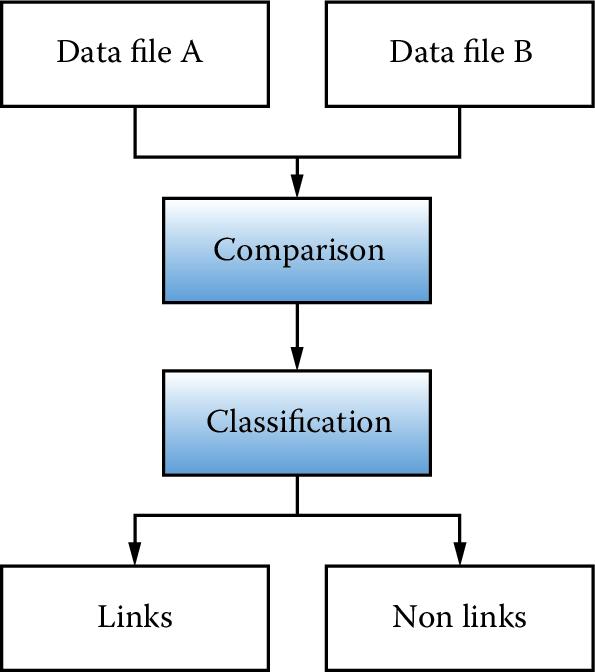
\includegraphics[width=0.7\linewidth]{ChapterLinkage/figures/fig3-1} 

}

\caption{The preprocessing pipeline}\label{fig:fig3-1}
\end{figure}

The canonical record linkage workflow process is shown in Figure
\ref{fig:fig3-1} for two data files, A and B. The goal is to identify
all pairs of records in the two data sets that correspond to the same
underlying individual. One approach is to compare all data units from
file A with all units in file B and classify all of the comparison
outcomes to decide whether or not the records match. In a perfect
statistical world the comparison would end with a clear determination of
links and nonlinks.

Alas, a perfect world does not exist, and there is likely to be noise in
the variables that are common to both data sets and that will be the
main identifiers for the record linkage. Although the original files A
and B are the starting point, the identifiers must be preprocessed
before they can be compared. Determining identifiers for the linkage and
deciding on the associated cleaning steps are extremely important, as
they result in a necessary reduction of the possible search space.

In the next section we begin our overview of the record linkage process
with a discussion of the main steps in data preprocessing. This is
followed by a section on approaches to record linkage that includes
rule-based, probabilistic, and machine learning algorithms. Next we
cover classification and evaluation of links, and we conclude with a
discussion of data privacy in record linkage.

\section{Preprocessing data for record
linkage}\label{preprocessing-data-for-record-linkage}

As noted in the introductory chapter, all data work involves
preprocessing, and data that need to be linked is no exception.
Preprocessing refers to a workflow that transforms messy, noisy, and
unstructured data into a well-defined, clearly structured, and
quality-tested data set. Elsewhere in this book, we discuss general
strategies for data preprocessing.\footnote{This topic (quality of data,
  preprocessing issues) is discussed in more detail in Section 1.4.} In
this section, we focus specifically on preprocessing steps relating to
the choice of input fields for the record linkage algorithm.
Preprocessing for any kind of a new data set is a complex and
time-consuming process because it is ``hands-on'': it requires judgment
and cannot be effectively automated. It may be tempting to minimize this
demanding work under the assumption that the record linkage algorithm
will account for issues in the data, but it is difficult to overstate
the value of preprocessing for record linkage quality. As Winkler notes:
``In situations of reasonably high-quality data, preprocessing can yield
a greater improvement in matching efficiency than string comparators and
`optimized' parameters. In some situations, 90\% of the improvement in
matching efficiency may be due to preprocessing'' (Winkler
\protect\hyperlink{ref-winkler09}{2009}).

The first step in record linkage is to develop link keys, which are the
record fields that will be used to predict link status. These can
include common identifiers like first and last name. Survey and
administrative data sets may include a number of clearly identifying
variables like address, birth date, and sex. Other data sets, like
transaction records or social media data, often will not include address
or birth date but may still include other identifying fields like
occupation, a list of interests, or connections on a social network.
Consider this chapter's illustrative example of the US Patent and
Trademark Office (USPTO) data (Ventura, Nugent, and Fuchs
\protect\hyperlink{ref-ventura2015seeing}{2015}):

\begin{quote}
USPTO maintains an online database of all patents issued in the United
States. In addition to identifying information about the patent, the
database contains each patent's list of inventors and assignees, the
companies, organizations, individuals, or government agencies towhich
the patent is assigned. \ldots{} However, inventors and assignees in the
USPTO database are not given unique identification numbers, making it
difficult to track inventors and assignees across their patents or link
their information to other data sources.
\end{quote}

There are some basic precepts that are useful when considering
identifying fields. The more different values a field can take, the less
likely it is that two randomly chosen individuals in the population will
agree on those values. Therefore, fields that exhibit a wider range of
values are more powerful as link keys: names are much better link keys
than sex or year of birth.

\begin{center}\rule{0.5\linewidth}{\linethickness}\end{center}

\textbf{Example: Link keys in practice}

``A Harvard professor has re-identified the names of more than 40
percent of a sample of anonymous participants in a high-profile DNA
study, highlighting the dangers that ever greater amounts of personal
data available in the Internet era could unravel personal secrets.
\ldots{} Of the 1,130 volunteers Sweeney and her team reviewed, about
579 provided zip code, date of birth and gender, the three key pieces of
information she needs to identify anonymous people combined with
information from voter rolls or other public records. Of these, Sweeney
succeeded in naming 241, or 42 percent of the total. The Personal Genome
Project confirmed that 97 percent of the names matched those in its
database if nicknames and first name variations were included'' (Tanner
\protect\hyperlink{ref-forbesharvard}{2013}).

\begin{center}\rule{0.5\linewidth}{\linethickness}\end{center}

Complex link keys like addresses can be broken down into components so
that the components can be compared independently of one another. This
way, errors due to data quality can be further isolated. For example,
assigning a single comparison value to the complex fields ``1600
Pennsylvania'' and ``160 Pennsylvania Ave'' is less informative than
assigning separate comparison values to the street number and street
name portions of those fields. A record linkage algorithm that uses the
decomposed field can make more nuanced distinctions by assigning
different weights to errors in each component.

Sometimes a data set can include different variants of a field, like
legal first name and nickname. In these cases match rates can be
improved by including all variants of the field in the record
comparison. For example, if only the first list includes both variants,
and the second list has a single ``first name'' field that could be
either a legal first name or a nickname, then match rates can be
improved by comparing both variants and then keeping the better of the
two comparison outcomes. It is important to remember, however, that some
record linkage algorithms expect field comparisons to be somewhat
independent. In our example, using the outcome from both comparisons as
separate inputs into the probabilistic model we describe below may
result in a higher rate of false negatives. If a record has the same
value in the legal name and nickname fields, and if that value happens
to agree with the first name field in the second file, then the
agreement is being double-counted. By the same token, if a person in the
first list has a nickname that differs significantly from their legal
first name, then a comparison of that record to the corresponding record
will unfairly penalize the outcome because at least one of those name
comparisons will show a low level of agreement.

Preprocessing serves two purposes in record linkage. First, to correct
for issues in data quality that we described above. Second, to account
for the different ways that the input files were generated, which may
result in the same underlying data being recorded on different scales or
according to different conventions.

Once preprocessing is finished, it is possible to start linking the
records in the different data sets. In the next section we describe a
technique to improve the efficiency of the matching step.

\hypertarget{S:indexing}{\section{Indexing and
blocking}\label{S:indexing}}

There is a practical challenge to consider when comparing the records in
two files. If both files are roughly the same size, say \(100\) records
in the first and \(100\) records in the second file, then there are
\(10{,}000\) possible comparisons, because the number of pairs is the
product of the number of records in each file. More generally, if the
number of records in each file is approximately \(n\), then the total
number of possible record comparisons is approximately \(n^2\). Assuming
that there are no duplicate records in the input files, the proportion
of record comparisons that correspond to a link is only \(1/n\). If we
naively proceed with all \(n^2\) possible comparisons, the linkage
algorithm will spend the bulk of its time comparing records that are not
matches. Thus it is possible to speed up record linkage significantly by
skipping comparisons between record pairs that are not likely to be
linked.

Indexing refers to techniques that determine which of the possible
comparisons will be made in a record linkage application. The most used
technique for indexing is blocking. In this approach you construct a
``blocking key'' for each record by concatenating fields or parts of
fields. Two records with identical blocking keys are said to be in the
same block, and only records in the same block are compared. This
technique is effective because performing an exact comparison of two
blocking keys is a relatively quick operation compared to a full record
comparison, which may involve multiple applications of a fuzzy string
comparator.

\begin{center}\rule{0.5\linewidth}{\linethickness}\end{center}

\textbf{Example: Blocking in practice}

Given two lists of individuals, one might construct the blocking key by
concatenating the first letter of the last name and the postal code and
then ``blocking'' on first character of last name and postal code. This
reduces the total number of comparisons by only comparing those
individuals in the two files who live in the same locality and whose
last names begin with the same letter.

\begin{center}\rule{0.5\linewidth}{\linethickness}\end{center}

There are important considerations when choosing the blocking key.
First, the choice of blocking key creates a potential bias in the linked
data because true matches that do not share the same blocking key will
not be found. In the example, the blocking strategy could fail to match
records for individuals whose last name changed or who moved. Second,
because blocking keys are compared exactly, there is an implicit
assumption that the included fields will not have typos or other data
entry errors. In practice, however, the blocking fields will exhibit
typos. If those typos are not uniformly distributed over the population,
then there is again the possibility of bias in the linked data
set\footnote{This topic is discussed in more detail in Chapter 10.}. One
simple strategy for dealing with imperfect blocking keys is to implement
multiple rounds of blocking and matching. After the first set of matches
is produced, a new blocking strategy is deployed to search for
additional matches in the remaining record pairs.

Blocking based on exact field agreements is common in practice, but
there are other approaches to indexing that attempt to be more error
tolerant. For example, one may use clustering algorithms to identify
sets of similar records. In this approach an index key, which is
analogous to the blocking key above, is generated for both data sets and
then the keys are combined into a single list. A distance function must
be chosen and pairwise distances computed for all keys. The clustering
algorithm is then applied to the combined list, and only record pairs
that are assigned to the same cluster are compared. This is a
theoretically appealing approach but it has the drawback that the
similarity metric has to be computed for all pairs of records. Even so,
computing the similarity measure for a pair of blocking keys is likely
to be cheaper than computing the full record comparison, so there is
still a gain in efficiency. Whang et al. (Whang et al.
\protect\hyperlink{ref-whang2009entity}{2009}) provide a nice review of
indexing approaches.

In addition to reducing the computational burden of record linkage,
indexing plays an important secondary role. Once implemented, the
fraction of comparisons made that correspond to true links will be
significantly higher. For some record linkage approaches that use an
algorithm to find optimal parameters---like the probabilistic
approach---having a larger ratio of matches to nonmatches will produce a
better result.

\section{Matching}\label{matching}

The purpose of a record linkage algorithm is to examine pairs of records
and make a prediction as to whether they correspond to the same
underlying entity. (There are some sophisticated algorithms that examine
sets of more than two records at a time (Steorts, Hall, and Fienberg
\protect\hyperlink{ref-steorts2014smered}{2014}), but pairwise
comparison remains the standard approach.) At the core of every record
linkage algorithm is a function that compares two records and outputs a
``score'' that quantifies the similarity between those records.
Mathematically, the match score is a function of the output from
individual field comparisons: agreement in the first name field,
agreement in the last name field, etc. Field comparisons may be
binary---indicating agreement or disagreement---or they may output a
range of values indicating different levels of agreement. There are a
variety of methods in the statistical and computer science literature
that can be used to generate a match score, including nearest-neighbor
matching, regression-based matching, and propensity score matching. The
probabilistic approach to record linkage defines the match score in
terms of a likelihood ratio (Fellegi and Sunter
\protect\hyperlink{ref-FS69}{1969}).

\begin{center}\rule{0.5\linewidth}{\linethickness}\end{center}

\textbf{Example: Matching in practice}

Long strings, such as assignee and inventor names, are susceptible to
typographical errors and name variations. For example, none of Sony
Corporation, Sony Corporatoin and Sony Corp. will match using simple
exact matching. Similarly, David vs.~Dave would not match (Ventura,
Nugent, and Fuchs \protect\hyperlink{ref-ventura2015seeing}{2015}).

\begin{center}\rule{0.5\linewidth}{\linethickness}\end{center}

Comparing fields whose values are continuous is straightforward: often
one can simply take the absolute difference as the comparison value.
Comparing character fields in a rigorous way is more complicated. For
this purpose, different mathematical definitions of the distance between
two character fields have been defined. Edit distance, for example, is
defined as the minimum number of edit operations---chosen from a set of
allowed operations---needed to convert one string to another. When the
set of allowed edit operations is single-character insertions,
deletions, and substitutions, the corresponding edit distance is also
known as the Levenshtein distance. When transposition of adjacent
characters is allowed in addition to those operations, the corresponding
edit distance is called the Levenshtein--Damerau distance.

Edit distance is appealing because of its intuitive definition, but it
is not the most efficient string distance to compute. Another standard
string distance known as Jaro--Winkler distance was developed with
record linkage applications in mind and is faster to compute. This is an
important consideration because in a typical record linkage application
most of the algorithm run time will be spent performing field
comparisons. The definition of Jaro--Winkler distance is less intuitive
than edit distance, but it works as expected: words with more characters
in common will have a higher Jaro--Winkler value than those with fewer
characters in common. The output value is normalized to fall between 0
and 1. Because of its history in record linkage applications, there are
some standard variants of Jaro--Winkler distance that may be implemented
in record linkage software. Some variants boost the weight given to
agreement in the first few characters of the strings being compared.
Others decrease the score penalty for letter substitutions that arise
from common typos.

Once the field comparisons are computed, they must be combined to
produce a final prediction of match status. In the following sections we
describe three types of record linkage algorithms: rule-based,
probabilistic, and machine learning.

\subsection{Rule-based approaches}\label{rule-based-approaches}

A natural starting place is for a data expert to create a set of ad hoc
rules that determine which pairs of records should be linked. In the
classical record linkage setting where the two files have a number of
identifying fields in common, this is not the optimal approach. However,
if there are few fields in common but each file contains auxiliary
fields that may inform a linkage decision, then an ad hoc approach may
be appropriate.

\begin{center}\rule{0.5\linewidth}{\linethickness}\end{center}

\textbf{Example: Linking in practice}

Consider the problem of linking two lists of individuals where both
lists contain first name, last name, and year of birth. Here is one
possible linkage rule: link all pairs of records such that

\begin{itemize}
\item
  the Jaro--Winkler comparison of first names is greater than 0.9
\item
  the Jaro--Winkler comparison of last names is greater than 0.9
\item
  the first three digits of the year of birth are the same.
\end{itemize}

The result will depend on the rate of data errors in the year of birth
field and typos in the name fields.

\begin{center}\rule{0.5\linewidth}{\linethickness}\end{center}

By \emph{auxiliary field} we mean data fields that do not appear on both
data sets, but which may nonetheless provide information about whether
records should be linked. Consider a situation in which the first list
includes an occupation field and the second list includes educational
history. In that case one might create additional rules to eliminate
matches where the education was deemed to be an unlikely fit for the
occupation.

This method may be attractive if it produces a reasonable-looking set of
links from intuitive rules, but there are several pitfalls. As the
number of rules grows it becomes harder to understand the ways that the
different rules interact to produce the final set of links. There is no
notion of a threshold that can be increased or decreased depending on
the tolerance for false positive and false negative errors. The rules
themselves are not chosen to satisfy any kind of optimality, unlike the
probabilistic and machine learning methods. Instead, they reflect the
practitioner's domain knowledge about the data sets.

\subsection{Probabilistic record
linkage}\label{probabilistic-record-linkage}

In this section we describe the probabilistic approach to record
linkage, also known as the Fellegi--Sunter algorithm (Fellegi and Sunter
\protect\hyperlink{ref-FS69}{1969}). This approach dominates in
traditional record linkage applications and remains an effective and
efficient way to solve the record linkage problem today.

In this section we give a somewhat formal definition of the statistical
model underlying the algorithm. By understanding this model, one is
better equipped to define link keys and record comparisons in an optimal
way.

\begin{center}\rule{0.5\linewidth}{\linethickness}\end{center}

\textbf{Example: Usefulness of probabilistic record linkage}

In practice, it is typically the case that a researcher will want to
combine two or more data sets containing records for the same
individuals or units that possibly come from different sources. Unless
the sources all contain the same unique identifiers, linkage will likely
require matching on standardized text strings. Even standardized data
are likely to contain small differences that preclude exact matching as
in the matching example above. The Census Bureau's Longitudinal Business
Database (LBD) links establishment records from administrative and
survey sources. Exact numeric identifiers do most of the heavy lifting,
but mergers, acquisitions, and other actions can break these linkages.
Probabilistic record linkage on company names and/or addresses is used
to fix these broken linkages that bias statistics on business dynamics
(Jarmin and Miranda
\protect\hyperlink{ref-jarmin2002longitudinal}{2002}).

\begin{center}\rule{0.5\linewidth}{\linethickness}\end{center}

Let \(A\) and \(B\) be two lists of individuals whom we wish to link.
The product set \(A \times B\) contains all possible pairs of records
where the first element of the pair comes from \(A\) and the second
element of the pair comes from \(B\). A fraction of these pairs will be
matches, meaning that both records in the pair represent the same
underlying individual, but the vast majority of them will be nonmatches.
In other words, \(A \times B\) is the disjoint union of the set of
matches \(M\) and the set of nonmatches \(U\), a fact that we denote
formally by \(A \times B = M \cup U\).

Let \(\gamma\) be a vector-valued function on \(A \times B\) such that,
for \(a \in A\) and \(b \in B\), \(\gamma(a, b)\) represents the outcome
of a set of field comparisons between \(a\) and \(b\). For example, if
both \(A\) and \(B\) contain data on individuals' first names, last
names, and cities of residence, then \(\gamma\) could be a vector of
three binary values representing agreement in first name, last name, and
city. In that case \(\gamma(a, b) = (1, 1, 0)\) would mean that the
records \(a\) and \(b\) agree on first name and last name, but disagree
on city of residence.

For this model, the comparison outcomes in \(\gamma(a, b)\) are not
required to be binary, but they do have to be categorical: each
component of \(\gamma(a, b)\) should take only finitely many values.
This means that a continuous comparison outcome---such as output from
the string comparator---has to be converted to an ordinal value
representing levels of agreement. For example, one might create a
three-level comparison, using one level for exact agreement, one level
for approximate agreement defined as a Jaro--Winkler score greater than
0.85, and one level for nonagreement corresponding to a Jaro--Winkler
score less than 0.85.

If a variable being used in the comparison has a significant number of
missing values, it can help to create a comparison outcome level to
indicate missingness. Consider two data sets that both have middle
initial fields, and suppose that in one of the data sets the middle
initial is filled in only about half of the time. When comparing
records, the case where both middle initials are filled in but are not
the same should be treated differently from the case where one of the
middle initials is blank, because the first case provides more evidence
that the records do not correspond to the same person. We handle this in
the model by defining a three-level comparison for the middle initial,
with levels to indicate ``equal,'' ``not equal,'' and ``missing.''

Probabilistic record linkage works by weighing the probability of seeing
the result \(\gamma(a, b)\) if \((a, b)\) belongs to the set of matches
\(M\) against the probability of seeing the result if \((a, b)\) belongs
to the set of nonmatches \(U\). Conditional on \(M\) or \(U\), the
distribution of the individual comparisons defined by \(\gamma\) are
assumed to be mutually independent. The parameters that define the
marginal distributions of \(\gamma | M\) are called
\emph{\(m\)-weights}, and similarly the marginal distributions of
\(\gamma | U\) are called \emph{\(u\)-weights}.

In order to apply the Fellegi--Sunter method, it is necessary to choose
values for these parameters, \(m\)-weights and \(u\)-weights. With
labeled data---a pair of lists for which the match status is known---it
is straightforward to solve for optimal values. Training data are not
usually available, however, and the typical approach is to use
expectation maximization to find optimal values.

We have noted that primary motivation for record linkage is to create a
linked data set for analysis that will have a richer than either of the
input data sets alone. A natural application is to perform a linear
regression using a combination of variables from both files as
predictors. With all record linkage approaches it is a challenge to
understand how errors from the linkage process will manifest in the
regression. Probabilistic record linkage has an advantage over
rule-based and machine learning approaches in that there are theoretical
results concerning coefficient bias and errors (Scheuren and Winkler
\protect\hyperlink{ref-scheuren1993regression}{1993}; Lahiri and Larsen
\protect\hyperlink{ref-lahiri2005regression}{2005}). More recently,
Chipperfield and Chambers have developed an approach based on the
bootstrap to account for record linkage errors when making inferences
for cross-tabulated

\subsection{Machine learning approaches to
linking}\label{machine-learning-approaches-to-linking}

Computer scientists have contributed extensively in parallel literature
focused on linking large data sets (Christen
\protect\hyperlink{ref-christen2012data}{2012}\protect\hyperlink{ref-christen2012data}{b}).
Their focus is on identifying potential links using approaches that are
fast and scalable, and approaches are developed based on work in network
algorithms and machine learning.

While simple blocking as described in Section
\protect\hyperlink{S:indexing}{Indexing and Blocking} is standard in
Fellegi--Sunter applications, computer scientists are likely to use the
more sophisticated clustering approach to indexing. Indexing may also
use network information to include, for example, records for individuals
that have a similar place in a social graph. When linking lists of
researchers, one might specify that comparisons should be made between
records that share the same address, have patents in the same patent
class, or have overlapping sets of coinventors. These approaches are
known as semantic blocking, and the computational requirements are
similar to standard blocking (Christen
\protect\hyperlink{ref-christen2012data}{2012}\protect\hyperlink{ref-christen2012data}{b}).

In recent years machine learning approaches\footnote{This topic is
  discussed in more detail in Chapter 6.} have been applied to record
linkage following their success in other areas of prediction and
classification. Computer scientists couch the analytical problem as one
of entity resolution, even though the conceptual problem is identical.
As Wick et al. (Wick et al. \protect\hyperlink{ref-wick2013joint}{2013})
note:

\begin{quote}
Entity resolution, the task of automatically determining which mentions
refer to the same real-world entity, is a crucial aspect of knowledge
base construction and management. However, performing entity resolution
at large scales is challenging because (1) the inference algorithms must
cope with unavoidable system scalability issues and (2) the search space
grows exponentially in the number of mentions. Current conventional
wisdom declares that performing coreference at these scales requires
decomposing the problem by first solving the simpler task of
entity-linking (matching a set of mentions to a known set of KB
entities), and then performing entity discovery as a post-processing
step (to identify new entities not present in the KB). However, we argue
that this traditional approach is harmful to both entity-linking and
overall coreference accuracy. Therefore, we embrace the challenge of
jointly modeling entity-linking and entity discovery as a single entity
resolution problem.
\end{quote}

Figure \ref{fig:fig3-2} provides a useful comparison between classical
record linkage and learning-based approaches. In machine learning there
is a predictive model and an algorithm for ``learning'' the optimal set
of parameters to use in the predictive algorithm. The learning algorithm
relies on a training data set. In record linkage, this would be a
curated data set with true and false matches labeled as such. See
(Ventura, Nugent, and Fuchs
\protect\hyperlink{ref-ventura2015seeing}{2015}) for an example and a
discussion of how a training data set was created for the problem of
disambiguating inventors in the USPTO database. Once optimal parameters
are computed from the training data, the predictive model can be applied
to unlabeled data to find new links. The quality of the training data
set is critical; the model is only as good as the data it is trained on.

\begin{figure}

{\centering 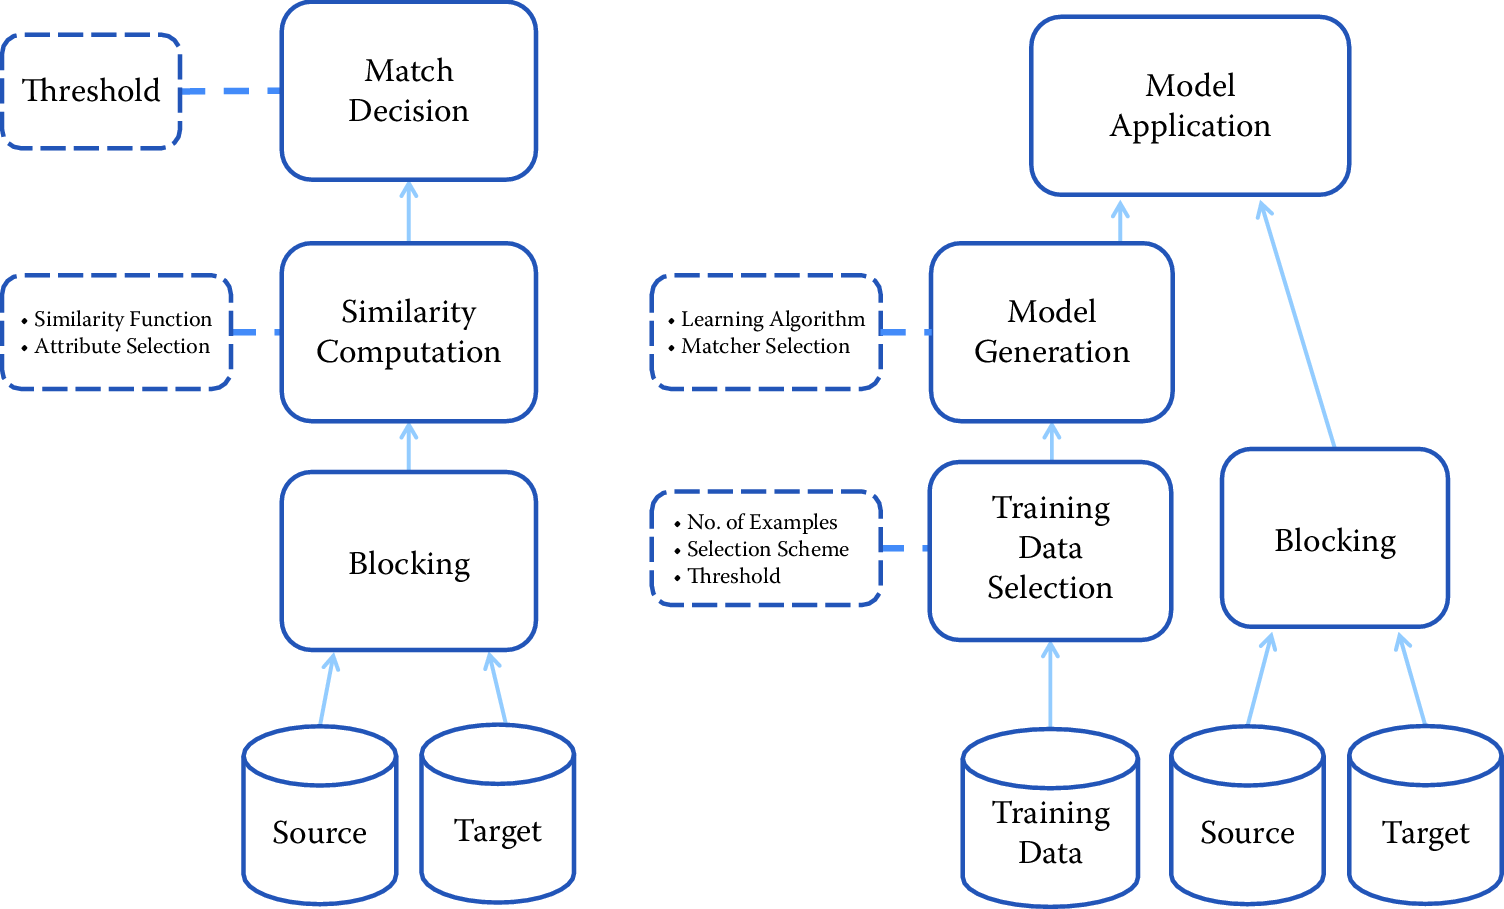
\includegraphics[width=0.7\linewidth]{ChapterLinkage/figures/fig3-2} 

}

\caption{Probabilistic (left) vs. machine learning (right) approaches to linking. Source: Köpcke et al. [@kopcke2010evaluation]}\label{fig:fig3-2}
\end{figure}

\vspace*{-6pt} An example of a machine learning model that is popular
for record linkage is the random forest model\footnote{See Chapter 6.}
(Breiman \protect\hyperlink{ref-Breiman01}{2001}). This is a
classification model that fits a large number of classification trees to
a labeled training data set. Each individual tree is trained on a
bootstrap sample of all labeled cases using a random subset of predictor
variables. After creating the classification trees, new cases are
labeled by giving each tree a vote and keeping the label that receives
the most votes. This highly randomized approach corrects for a problem
with simple classification trees, which is that they may overfit to
training data.

As shown in Figure \ref{fig:fig3-2}, a major difference between
probabilistic and machine learning approaches is the need for labeled
training data to implement the latter approach. Usually training data
are created through a painstaking process of clerical review. After an
initial round of record linkage, a sample of record pairs that are not
clearly matches or nonmatches is given to a research assistant who makes
the final determination. In some cases it is possible to create training
data by automated means. For example, when there is a subset of the
complete data that contains strongly identifying fields. Suppose that
both of the candidate lists contain name and date of birth fields and
that in the first list the date of birth data are complete, but in the
second list only about 10\% of records contain date of birth. For
reasonably sized lists, name and date of birth together will be a nearly
unique identifier. It is then possible to perform probabilistic record
linkage on the subset of records with date of birth and be confident
that the error rates would be small. If the subset of records with date
of birth is representative of the complete data set, then the output
from the probabilistic record linkage can be used as ``truth'' data.

\enlargethispage{12pt} Given a quality training data set, machine
learning approaches may have advantages over probabilistic record
linkage. Consider the random forest model. Random forests are more
robust to correlated predictor variables, because only a random subset
of predictors is included in any individual classification tree. The
conditional independence assumption, to which we alluded in our
discussion of the probabilistic model, can be dropped. An estimate of
the generalization error can be computed in the form of ``out-of-bag
error.'' A measure of variable importance is computed that gives an idea
of how powerful a particular field comparison is in terms of correctly
predicting link status. Finally, unlike the Fellegi--Sunter model,
predictor variables can be continuous.

The combination of being robust to correlated variables and providing a
variable importance measure makes random forests a useful diagnostic
tool for record linkage models. It is possible to refine the record
linkage model iteratively, by first including many predictor variables,
including variants of the same comparison, and then using the variable
importance measure to narrow down the predictors to a parsimonious set.

There are many published studies on the effectiveness of random forests
and other machine learning algorithms for record linkage. Christen and
Ahmed et al. provide some pointers (Christen
\protect\hyperlink{ref-christen2012survey}{2012}\protect\hyperlink{ref-christen2012survey}{a};
Elmagarmid, Ipeirotis, and Verykios
\protect\hyperlink{ref-elmagarmid2007duplicate}{2007}).

\vspace*{-3pt}

\subsection{Disambiguating networks}\label{disambiguating-networks}

\enlargethispage{18pt} The problem of disambiguating entities in a
network is closely related to record linkage: in both cases the goal is
to consolidate multiple records corresponding to the same entity. Rather
than finding the same entity in two data sets, however, the goal in
network disambiguation is to consolidate duplicate records in a network
data set. By network we mean that the data set contains not only typical
record fields like names and addresses but also information about how
entities relate to one another: entities may be coauthors, coinventors,
or simply friends in a social network.

The record linkage techniques that we have described in this chapter can
be applied to disambiguate a network. To do so, one must convert the
network to a form that can be used as input into a record linkage
algorithm. For example, when disambiguating a social network one might
define a field comparison whose output gives the fraction of friends in
common between two records. Ventura et al. demonstrated the relative
effectiveness of the probabilistic method and machine learning
approaches to disambiguating a database of inventors in the USPTO
database (Ventura, Nugent, and Fuchs
\protect\hyperlink{ref-ventura2015seeing}{2015}). Another approach is to
apply clustering algorithms from the computer science literature to
identify groups of records that are likely to refer to the same entity.
Huang et al. (Huang, Ertekin, and Giles
\protect\hyperlink{ref-HEG06}{2006}) have developed a successful method
based on an efficient computation of distance between individuals in the
network. These distances are then fed into the DBSCAN clustering
algorithm to identify unique entities.

\vspace*{-3pt}

\section{Classification}\label{classification}

Once the match score for a pair of records has been computed using the
probabilistic or random forest method, a decision has to be made whether
the pair should be linked. This requires classifying the pair as either
a ``true'' or a ``false'' match. In most cases, a third classification
is required---sending for manual review and classification.

\subsection{Thresholds}\label{S:thresholds}

In the probabilistic and random forest approaches, both of which output
a ``match score'' value, a classification is made by establishing a
threshold \(T\) such that all records with a match score greater than
\(T\) are declared to be links. Because of the way these algorithms are
defined, the match scores are not meaningful by themselves and the
threshold used for one linkage application may not be appropriate for
another application. Instead, the classification threshold must be
established by reviewing the model output.

Typically one creates an output file that includes pairs of records that
were compared along with the match score. The file is sorted by match
score and the reviewer begins to scan the file from the highest match
scores to the lowest. For the highest match scores the record pairs will
agree on all fields and there is usually no question about the records
being linked. However, as the scores decrease the reviewer will see more
record pairs whose match status is unclear (or that are clearly
nonmatches) mixed in with the clear matches. There are a number of ways
to proceed, depending on the resources available and the goal of the
project.

Rather than set a single threshold, the reviewer may set two thresholds
\(T_1 > T_2\). Record pairs with a match score greater than \(T_1\) are
marked as matches and removed from further consideration. The set of
record pairs with a match score between \(T_1\) and \(T_2\) are believed
to contain significant numbers of matches and nonmatches. These are sent
to clerical review, meaning that research assistants will make a final
determination of match status. The final set of links will include clear
matches with a score greater than \(T_1\) as well as the record pairs
that pass clerical review. If the resources are available for this
approach and the initial threshold \(T_1\) is set sufficiently high,
then the resulting data set will contain a minimal number of false
positive links. The collection of record pairs with match scores between
\(T_1\) and \(T_2\) is sometimes referred to as the clerical review
region.

The clerical review region generally contains many more pairs than the
set of clear matches, and it can be expensive and time-consuming to
review each pair. Therefore, a second approach is to establish tentative
threshold \(T\) and send only a sample of record pairs with scores in a
neighborhood of \(T\) to clerical review. This results in data on the
relative numbers of true matches and true nonmatches at different score
levels, as well as the characteristics of record pairs that appear at a
given level. Based on the review and the relative tolerance for false
positive errors and false negative errors, a final threshold \(T'\) is
set such that pairs with a score greater than \(T'\) are considered to
be matches.

After viewing the results of the clerical review, it may be determined
that the parameters to the record linkage algorithm could be improved to
create a clearer delineation between matches and nonmatches. For
example, a research assistant may determine that many potential false
positives appear near the tentative threshold because the current set of
record linkage parameters is giving too much weight to agreement in
first name. In this case the reviewer may decide to update the record
linkage model to produce an improved set of match scores. The update may
consist in an ad hoc adjustment of parameters, or the result of the
clerical review may be used as training data and the parameter-fitting
algorithm may be run again. An iterative approach like this is common
when first linking two data sets because the clerical review process can
improve one's understanding of the data sets involved.

Setting the threshold value higher will reduce the number of false
positives (record pairs for which a link is incorrectly predicted) while
increasing the number of false negatives (record pairs that should be
linked but for which a link is not predicted). The proper tradeoff
between false positive and false negative error rates will depend on the
particular application and the associated loss function, but there are
some general concerns to keep in mind. Both types of errors create bias,
which can impact the generalizability of analyses conducted on the
linked data set. Consider a simple regression on the linked data that
includes fields from both data sets. If the threshold is too high, then
the linked data will be biased toward records with no data entry errors
or missing values, and whose fields did not change over time. This set
of records may not be representative of the population as a whole. If a
low threshold is used, then the set of linked records will contain more
pairs that are not true links and the variables measured in those
records are independent of each other. Including these records in a
regression amounts to adding statistical noise to the data.

\subsection{One-to-one links}\label{one-to-one-links}

In the probabilistic and machine learning approaches to record linkage
that we have described, each record pair is compared and a link is
predicted independently of all other record pairs. Because of the
independence of comparisons, one record in the first file may be
predicted to link to multiple records in the second file. Under the
assumption that each input file has been deduplicated, at most one of
these predictions can correspond to a true link. For many applications
it is preferable to extract a set of ``best'' links with the property
that each record in one file links to at most one record in the second
file. A set of links with this property is said to be one-to-one.

\enlargethispage{12pt} One possible definition of ``best'' is a set of
one-to-one links such that the sum of the match scores of all included
links is maximal. This is an example of what is known as the
\emph{assignment problem} in combinatorial optimization. In the linear
case above, where we care about the sum of match scores, the problem can
be solved exactly using the Hungarian algorithm (Kuhn
\protect\hyperlink{ref-kuhn2005hungarian}{2005})\footnote{This topic is
  discussed in more detail in Chapter 6.}.

\section{Record linkage and data
protection}\label{record-linkage-and-data-protection}

In many social science applications data sets there is no need for data
to include identifying fields like names and addresses. These fields may
be left out intentionally out of concern for privacy\footnote{See
  Chapter 11.}, or they may simply be irrelevant to the research
question. For record linkage, however, names and addresses are among the
best possible identifiers. We describe two approaches to the problem of
balancing needs for both effective record linkage and privacy.

The first approach is to establish a trusted third party or safe center.
The concept of trusted third parties (TTPs) is well known in
cryptography. In the case of record linkage, a third party takes a place
between the data owners and the data users, and it is this third party
that actually performs the linkage work. Both the data owners and data
users trust the third party in the sense that it assumes responsibility
for data protection (data owners) and data competence (data users) at
the same time. No party other than the TTP learns about the private data
of the other parties. After record linkage only the linked records are
revealed, with no identifiers attached. The TTP ensures that the
released linked data set cannot be relinked to any of the source data
sets. Possible third parties are safe centers, which are operated by
lawyers, or official trusted institutions like the US Census Bureau.
Some countries like the UK and Germany are establishing new institutions
specifically to act as TTPs for record linkage work.

The second approach is known as privacy-preserving record linkage. The
goal of this approach is to find the same individual in separate data
files without revealing the identity of the individual (Clifton et al.
\protect\hyperlink{ref-Clifton06}{2006}). In privacy-preserving record
linkage, cryptographic procedures are used to encrypt or hash
identifiers before they are shared for record linkage. Many of these
procedures require exact matching of the identifiers, however, and do
not tolerate any errors in the original identifiers. This leads to
information loss because it is not possible to account for typos or
other small variations in hashed fields. To account for this, Schnell
has developed a method to calculate string similarity of encrypted
fields using bloom filters (Schnell
\protect\hyperlink{ref-schnell2014efficient}{2014}; Schnell, Bachteler,
and Reiher \protect\hyperlink{ref-schnell2009privacy}{2009}).

In many countries these approaches are combined. For example, when the
UK established the ADRN, the latter established the concept of trusted
third parties. That third party is provided with data in which
identifying fields have been hashed. This solves the challenge of trust
between the different parties. Some authors argue that transparency of
data use and informed consent will help to build trust. In the context
of big data this is more challenging\footnote{This topic is discussed in
  more detail in Chapter 11.}.

\section{Summary}\label{summary}

Accurate record linkage is critical to creating high-quality data sets
for analysis. However, outside of a few small centers for record linkage
research, linking data sets historically relied on artisan approaches,
particularly for parsing and cleaning data sets. As the creation and use
of big data increases, so does the need for systematic record linkage.
The history of record linkage is long by computer science standards, but
new data challenges encourage the development of new approaches like
machine learning methods, clustering algorithms, and privacy-preserving
record linkage.

Record linkage stands on the boundary between statistics, information
technology, and privacy. We are confident that there will continue to be
exciting developments in this field in the years to come.

\section{Resources}\label{resources}

Out of many excellent resources on the subject, we note the following:

\begin{itemize}
\item
  We strongly recommend Christen's book (Christen
  \protect\hyperlink{ref-christen2012data}{2012}\protect\hyperlink{ref-christen2012data}{b}).
\item
  There is a wealth of information available on the ADRN website
  (Economic and Social Research Council
  \protect\hyperlink{ref-EconomicandSocialResearchCouncil2016}{2016}).
\item
  Winkler has a series of high-quality survey articles (Winkler
  \protect\hyperlink{ref-WICS:WICS1317}{2014}).
\item
  The German Record Linkage Center is a resource for research, software,
  and ongoing conference activities (Schnell
  \protect\hyperlink{ref-Schnell2016}{2016}).
\end{itemize}

\hypertarget{chap:db}{\chapter{Databases}\label{chap:db}}

\textbf{Ian Foster and Pascal Heus}

Once the data have been collected and linked into different files, it is
necessary to store and organize them. Social scientists are used to
working with one analytical file, often in SAS, Stata, SPSS, or R. This
chapter, which may be the most important chapter in the book, describes
different approaches to storing data in ways that permit rapid and
reliable exploration and analysis.

\section{Introduction}\label{sec:db:intro}

We turn now to the question of how to store, organize, and manage the
data used in data-intensive social science. As the data with which you
work grow in volume and diversity, effective data management becomes
increasingly important if you are to avoid issues of scale and
complexity from overwhelming your research processes. In particular,
when you deal with data that get frequently updated, with changes made
by different people, you will frequently want to use database management
systems (DBMSs) instead of maintaining data in single files or within
siloed statistical packages such as SAS, SPSS, Stata, and R. Indeed, we
go so far as to say: if you take away \emph{just one thing} from this
book, it should be this: \emph{Use a database!}

As we explain in this chapter, DBMSs provide an environment that greatly
simplifies data management and manipulation. They require a little bit
of effort to set up, but are worth it. They permit large amounts of data
to be organized in multiple ways that allow for efficient and rapid
exploration via powerful declarative query languages; durable and
reliable storage, via transactional features that maintain data
consistency; scaling to large data sizes; and intuitive analysis, both
within the DBMS itself and via bridges to other data analysis packages
and tools when specialized analyses are required. DBMSs have become a
critical component of a great variety of applications, from handling
transactions in financial systems to delivering data as a service to
power websites, dashboards, and applications. If you are using a
production-level enterprise system, chances are there is a database in
the back end. They are multi-purpose and well suited for organizing
social science data and for supporting analytics for data exploration.

DBMSs make many easy things trivial, and many hard things easy. They are
easy to use but can appear daunting to those unfamiliar with their
concepts and workings. A basic understanding of databases and of when
and how to use DBMSs is an important element of the social data
scientist's knowledge base. We therefore provide in this chapter an
introduction to databases and how to use them. We describe different
types of databases and their various features, and how different types
can be applied in different contexts. We describe basic features like
how to get started, set up a database schema, ingest data, query data
within a database, and get results out. We also discuss how to link from
databases to other tools, such as Python, R, and Stata (if you really
have to). Chapter~{[}Programming with Big Data{]} describes how to apply
parallel computing methods when needed.

\hypertarget{sec:db:when}{\section{DBMS: When and
why}\label{sec:db:when}}

Consider the following three data sets:

\begin{enumerate}
\def\labelenumi{\arabic{enumi}.}
\item
  10,000 records describing research grants, each specifying the
  principal investigator, institution, research area, proposal title,
  award date, and funding amount in comma-separated-value (CSV) format.
\item
  10 million records in a variety of formats from funding agencies, web
  APIs, and institutional sources describing people, grants, funding
  agencies, and patents.
\item
  10 billion Twitter messages and associated metadata---around 10
  terabytes (\(10^{13}\) bytes) in total, and increasing at a terabyte a
  month.
\end{enumerate}

Which tools should you use to manage and analyze these data sets? The
answer depends on the specifics of the data, the analyses that you want
to perform, and the life cycle within which data and analyses are
embedded. Table \ref{tab:table4-1} summarizes relevant factors, which we
now discuss.

\begin{longtable}[]{@{}l@{}}
\caption{\label{tab:table4-1} When to use different data management and
analysis technologies}\tabularnewline
\toprule
\textbf{When to use different data management and analysis
technologies}\tabularnewline
\midrule
\endfirsthead
\toprule
\textbf{When to use different data management and analysis
technologies}\tabularnewline
\midrule
\endhead
\textbf{Text files, spreadsheets, and scripting language}\tabularnewline
• Your data are small\tabularnewline
• Your analysis is simple\tabularnewline
• You do not expect to repeat analyses over time\tabularnewline
\textbf{Statistical packages}\tabularnewline
• Your data are modest in size\tabularnewline
• Your analysis maps well to your chosen statistical
package\tabularnewline
\textbf{Relational database}\tabularnewline
• Your data are structured\tabularnewline
• Your data are large\tabularnewline
• You will be analyzing changed versions of your data over
time\tabularnewline
• You want to share your data and analyses with others\tabularnewline
\textbf{NoSQL database}\tabularnewline
• Your data are unstructured\tabularnewline
• Your data are extremely large\tabularnewline
\bottomrule
\end{longtable}

\vspace*{-8pt} In the case of data set~1 (10,000 records describing
research grants), it may be feasible to leave the data in their original
file, use spreadsheets, pivot tables, or write programs in
\textbf{scripting languages}\footnote{A scripting language is a
  programming language used to automate tasks that could otherwise be
  performed one by one by the user.} such as Python or R to ask
questions of those files. For example, someone familiar with such
languages can quickly create a script to extract from data set~1 all
grants awarded to one investigator, compute average grant size, and
count grants made each year in different areas.

However, this approach also has disadvantages. Scripts do not provide
inherent control over the file structure. This means that if you obtain
new data in a different format, your scripts need to be updated. You
cannot just run them over the newly acquired file. Scripts can also
easily become unreasonably slow as data volumes grow. A Python or R
script will not take long to search a list of 1,000 grants to find those
that pertain to a particular institution. But what if you have
information about 1 million grants, and for each grant you want to
search a list of 100,000 investigators, and for each investigator, you
want to search a list of 10 million papers to see whether that
investigator is listed as an author of each paper? You now have
\(1{,}000{,}000 \times 100{,}000 \times 10{,}000{,}000 = 10^{18}\)
comparisons to perform. Your simple script may now run for hours or even
days. You can speed up the search process by constructing indices, so
that, for example, when given a grant, you can find the associated
investigators in constant time rather than in time proportional to the
number of investigators. However, the construction of such indices is
itself a time-consuming and error-prone process.

For these reasons, the use of scripting languages alone for data
analysis is rarely to be recommended. This is not to say that all
analysis computations can be performed in database systems. A
programming language will also often be needed. But many data access and
manipulation computations are best handled in a database.

Researchers in the social sciences frequently use \textbf{statistical
packages}\footnote{A statistical package is a specialized compute
  program for analysis in statistics and economics.} such as R, SAS,
SPSS, and Stata for data analysis. Because these systems integrate some
crude data management, statistical analysis, and graphics capabilities
in a single package, a researcher can often carry out a data analysis
project of modest size within the same environment. However, each of
these systems has limitations that hinder its use for modern social
science research, especially as data grow in size and complexity.

Take Stata, for example. Stata always loads the entire data set into the
computer's working memory, and thus you would have no problems loading
data set~1. However, depending on your computer's memory, it could have
problems dealing with with data set~2 and certainly would not be able to
handle data set~3. In addition, you would need to perform this data
loading step each time you start working on the project, and your
analyses would be limited to what Stata can do. SAS can deal with larger
data sets, but is renowned for being hard to learn and use. Of course
there are workarounds in statistical packages. For example, in Stata you
can deal with larger file sizes by choosing to only load the variables
or cases that you need for the analysis (Kohler and Kreuter
\protect\hyperlink{ref-kohler2012datenanalyse}{2012}). Likewise, you can
deal with more complex data by creating a system of files that each can
be linked as needed for a particular analysis through a common
identifier variable\footnote{For example, the Panel Study of Income
  Dynamics {[}181{]} has a series of files that are related and can be
  combined through common identifier variables {[}182{]}.}.

Those solutions essentially mimic core functions of a DBMS, and you
would be well advised to set up such system, especially if you find
yourself in a situation where the data set is constantly updated through
different users, if groups of users have different rights to use your
data or should only have access to subsets of the data, and if the
analysis takes place on a server that sends results to a client
(browser). Statistics packages also have difficulty working with more
than one data source at a time---something that DBMSs are designed to do
well.

These considerations bring us to the topic of this chapter, namely
\textbf{database management systems}. A DBMS\footnote{DBMS is a system
  that interacts with users, other applications, and the database itself
  to capture and analyze data.} handles all of the issues listed above,
and more. As we will see below when we look at concrete examples, a DBMS
allows the programmer to define a logical design that fits the structure
of their data. The DBMS then a \emph{data model} (more on this below)
that allows these data to be stored, queried, and updated efficiently
and reliably on disk, thus providing independence from underlying
physical storage. It supports efficient access to data through
\emph{query languages} and automatic optimization of those queries to
permit fast analysis. Importantly, it also support concurrent access by
multiple users, which is not an option for file-based data storage. It
supports \emph{transactions}, meaning that any update to a database is
performed in its entirety or not at all, even in the face of computer
failures or multiple concurrent updates. And it reduces the time spent
both by analysts, by making it easy to express complex analytical
queries concisely, and on data administration, by providing simple and
uniform data administration interfaces.

A \emph{database} is a structured collection of data about entities and
their relationships. It models real-world objects---both entities (e.g.,
grants, investigators, universities) and relationships (e.g., ``Steven
Weinberg'' works at ``University of Texas at Austin'')---and captures
structure in ways that allow these entities and relationships to be
queried for analysis. A \emph{database management system} is a software
suite designed to safely store and efficiently manage databases, and to
assist with the maintenance and discovery of the relationships that
database represents. In general, a DBMS encompasses three key
components, as shown in Table \ref{tab:table4-2}: its \emph{data model}
(which defines how data are represented: see Box 4.1, its \emph{query
language} (which defines how the user interacts with the data), and
support for \emph{transactions and crash recovery} (to ensure reliable
execution despite system failures).\footnote{Some key DBMS features are
  often lacking in standard statistical packages: a standard query
  language (with commands that allow analyses or data manipulation on a
  subgroup of cases defined during the analysis, for example ``group by
  \ldots{},'' ``order by \ldots{}''), keys (for speed improvement), and
  an explicit model of a relational data structure.}

\begin{F00}
\textbf{Box 4.1: Data model} A \emph{data model} specifies the data
elements associated with a problem domain, the properties of those data
elements, and how those data elements relate to one another. In
developing a data model, we commonly first identity the entities that
are to be modeled and then define their properties and relationships.
For example, when working on the science of science policy (see
Figure~\ref{fig:fig2}, the entities include people, products,
institutions, and funding, each of which has various properties (e.g.,
for a person, their name, address, employer); relationships include ``is
employed by'' and ``is funded by.'' This conceptual data model can then
be translated into relational tables or some other database
representation, as we describe next.
\end{F00}

\begin{longtable}[]{@{}lccc@{}}
\caption{\label{tab:table4-2} Key components of a DBMS}\tabularnewline
\toprule
\begin{minipage}[b]{0.07\columnwidth}\raggedright\strut
\strut
\end{minipage} & \begin{minipage}[b]{0.32\columnwidth}\centering\strut
\textbf{Data model}\strut
\end{minipage} & \begin{minipage}[b]{0.31\columnwidth}\centering\strut
\textbf{Query language}\strut
\end{minipage} & \begin{minipage}[b]{0.19\columnwidth}\centering\strut
\textbf{Transactios, crash recovery}\strut
\end{minipage}\tabularnewline
\midrule
\endfirsthead
\toprule
\begin{minipage}[b]{0.07\columnwidth}\raggedright\strut
\strut
\end{minipage} & \begin{minipage}[b]{0.32\columnwidth}\centering\strut
\textbf{Data model}\strut
\end{minipage} & \begin{minipage}[b]{0.31\columnwidth}\centering\strut
\textbf{Query language}\strut
\end{minipage} & \begin{minipage}[b]{0.19\columnwidth}\centering\strut
\textbf{Transactios, crash recovery}\strut
\end{minipage}\tabularnewline
\midrule
\endhead
\begin{minipage}[t]{0.07\columnwidth}\raggedright\strut
User-facing\strut
\end{minipage} & \begin{minipage}[t]{0.32\columnwidth}\centering\strut
For example: relational, semi-structured\strut
\end{minipage} & \begin{minipage}[t]{0.31\columnwidth}\centering\strut
For example: SQL (for relational), XPath (for semi-structured)\strut
\end{minipage} & \begin{minipage}[t]{0.19\columnwidth}\centering\strut
Transactions\strut
\end{minipage}\tabularnewline
\begin{minipage}[t]{0.07\columnwidth}\raggedright\strut
Internal\strut
\end{minipage} & \begin{minipage}[t]{0.32\columnwidth}\centering\strut
Mapping data to storage systems; creating and maintaining indices\strut
\end{minipage} & \begin{minipage}[t]{0.31\columnwidth}\centering\strut
Query optimization and evaluation; consistency\strut
\end{minipage} & \begin{minipage}[t]{0.19\columnwidth}\centering\strut
Locking, concurrency control, recovery\strut
\end{minipage}\tabularnewline
\bottomrule
\end{longtable}

\vspace*{12pt} Literally hundreds of different open source, commercial,
and cloud-hosted versions DBMSs are available. However, you only need to
understand a relatively small number of concepts and major database
types to make sense of this diversity. Table \ref{tab:table4-3} defines
the major classes of DBMSs that we will consider in this book. We
consider only a few of these in any detail.

Relational DBMSs are the most widely used and mature systems, and will
be the optimal solution for many social science data analysis purposes.
We describe relational DBMSs in detail below, but in brief, they allow
for the efficient storage, organization, and analysis of large
quantities of \emph{tabular} data\footnote{Sometimes, as discussed in
  Chapter 3, the links are one to one and sometimes one to many.}: data
organized as tables, in which rows represent entities (e.g., research
grants) and columns represent attributes of those entities (e.g.,
principal investigator, institution, funding level). The associated
Structured Query Language (SQL) can then be used to perform a wide range
of analyses, which are executed with high efficiency due to
sophisticated indexing and query planning techniques.

\enlargethispage{-12pt} While relational DBMSs have dominated the
database world for decades, other database technologies have become
popular for various classes of applications in recent years. As we will
see, these alternative NoSQL DBMSs have typically been motivated by a
desire to scale the quantities of data and/or number of users that can
be supported and/or to deal with unstructured data that are not easily
represented in tabular form. For example, a key--value store can
organize large numbers of records, each of which associates an arbitrary
key with an arbitrary value. These stores, and in particular variants
called \emph{document stores} that permit text search on the stored
values, are widely used to organize and process the billions of records
that can be obtained from web crawlers. We review below some of these
alternatives and the factors that may motivate their~use.

\begin{longtable}[]{@{}lllll@{}}
\caption{\label{tab:table4-3} Types of databases: relational (first row) and
various types of NoSQL (other rows)}\tabularnewline
\toprule
\begin{minipage}[b]{0.07\columnwidth}\raggedright\strut
\textbf{Type}\strut
\end{minipage} & \begin{minipage}[b]{0.16\columnwidth}\raggedright\strut
\textbf{Examples}\strut
\end{minipage} & \begin{minipage}[b]{0.22\columnwidth}\raggedright\strut
\textbf{Advantages}\strut
\end{minipage} & \begin{minipage}[b]{0.20\columnwidth}\raggedright\strut
\textbf{Disadvantages}\strut
\end{minipage} & \begin{minipage}[b]{0.21\columnwidth}\raggedright\strut
\textbf{Uses}\strut
\end{minipage}\tabularnewline
\midrule
\endfirsthead
\toprule
\begin{minipage}[b]{0.07\columnwidth}\raggedright\strut
\textbf{Type}\strut
\end{minipage} & \begin{minipage}[b]{0.16\columnwidth}\raggedright\strut
\textbf{Examples}\strut
\end{minipage} & \begin{minipage}[b]{0.22\columnwidth}\raggedright\strut
\textbf{Advantages}\strut
\end{minipage} & \begin{minipage}[b]{0.20\columnwidth}\raggedright\strut
\textbf{Disadvantages}\strut
\end{minipage} & \begin{minipage}[b]{0.21\columnwidth}\raggedright\strut
\textbf{Uses}\strut
\end{minipage}\tabularnewline
\midrule
\endhead
\begin{minipage}[t]{0.07\columnwidth}\raggedright\strut
Relational database\strut
\end{minipage} & \begin{minipage}[t]{0.16\columnwidth}\raggedright\strut
MySQL, PostgreSQL, Oracle, SQL Server, Teradata\strut
\end{minipage} & \begin{minipage}[t]{0.22\columnwidth}\raggedright\strut
Consistency (ACID)\strut
\end{minipage} & \begin{minipage}[t]{0.20\columnwidth}\raggedright\strut
Fixed schema; typically harder to scale\strut
\end{minipage} & \begin{minipage}[t]{0.21\columnwidth}\raggedright\strut
Transactional systems: order processing, retail, hospitals, etc.\strut
\end{minipage}\tabularnewline
\begin{minipage}[t]{0.07\columnwidth}\raggedright\strut
Key--value store\strut
\end{minipage} & \begin{minipage}[t]{0.16\columnwidth}\raggedright\strut
Dynamo, Redis\strut
\end{minipage} & \begin{minipage}[t]{0.22\columnwidth}\raggedright\strut
Dynamic schema; easy scaling; high throughput\strut
\end{minipage} & \begin{minipage}[t]{0.20\columnwidth}\raggedright\strut
Not immediately consistent; no higher-level queries\strut
\end{minipage} & \begin{minipage}[t]{0.21\columnwidth}\raggedright\strut
Web applications\strut
\end{minipage}\tabularnewline
\begin{minipage}[t]{0.07\columnwidth}\raggedright\strut
Column store\strut
\end{minipage} & \begin{minipage}[t]{0.16\columnwidth}\raggedright\strut
Cassandra, HBase\strut
\end{minipage} & \begin{minipage}[t]{0.22\columnwidth}\raggedright\strut
Same as key--value; distributed; better compression at column
level\strut
\end{minipage} & \begin{minipage}[t]{0.20\columnwidth}\raggedright\strut
Not immediately consistent; using all columns is inefficient\strut
\end{minipage} & \begin{minipage}[t]{0.21\columnwidth}\raggedright\strut
Large-scale analysis\strut
\end{minipage}\tabularnewline
\begin{minipage}[t]{0.07\columnwidth}\raggedright\strut
Document store\strut
\end{minipage} & \begin{minipage}[t]{0.16\columnwidth}\raggedright\strut
CouchDB, MongoDB\strut
\end{minipage} & \begin{minipage}[t]{0.22\columnwidth}\raggedright\strut
Index entire document (JSON)\strut
\end{minipage} & \begin{minipage}[t]{0.20\columnwidth}\raggedright\strut
Not immediately consistent; no higher-level queries\strut
\end{minipage} & \begin{minipage}[t]{0.21\columnwidth}\raggedright\strut
Web applications\strut
\end{minipage}\tabularnewline
\begin{minipage}[t]{0.07\columnwidth}\raggedright\strut
Graph database\strut
\end{minipage} & \begin{minipage}[t]{0.16\columnwidth}\raggedright\strut
Neo4j, InfiniteGraph\strut
\end{minipage} & \begin{minipage}[t]{0.22\columnwidth}\raggedright\strut
Graph queries are fast\strut
\end{minipage} & \begin{minipage}[t]{0.20\columnwidth}\raggedright\strut
Difficult to do non-graph analysis\strut
\end{minipage} & \begin{minipage}[t]{0.21\columnwidth}\raggedright\strut
Recommendation systems, networks, routing\strut
\end{minipage}\tabularnewline
\bottomrule
\end{longtable}

Relational and NoSQL databases (and indeed other solutions, such as
statistical packages) can also be used together. Consider, for example,
Figure~\ref{fig:figdb-dbs}, which depicts data flows commonly
encountered in large research projects. Diverse data are being collected
from different sources: JSON documents from web APIs, web pages from web
scraping, tabular data from various administrative databases, Twitter
data, and newspaper articles. There may be hundreds or even thousands of
data sets in total, some of which may be extremely large. We initially
have no idea of what \textbf{schema}\footnote{A schema defines the
  structure of a database in a formal language defined by the DBMS. See
  Section 4.3.3.} to use for the different data sets, and indeed it may
not be feasible to define a unified set of schema, so diverse are the
data and so rapidly are new data sets being acquired. Furthermore, the
way we organize the data may vary according to our intended purpose. Are
we interested in geographic, temporal, or thematic relationships among
different entities? Each type of analysis may require a
differentorganization.

\enlargethispage{-12pt} For these reasons, a common storage solution is
to first load all data into a large NoSQL database. This approach makes
all data available via a common (albeit limited) query interface.
Researchers can then extract from this database the specific elements
that are of interest for their work, loading those elements into a
relational DBMS, another specialized DBMS (e.g., a graph database), or a
package for more detailed analysis. As part of the process of loading
data from the NoSQL database into a relational database, the researcher
will necessarily define schemas, relationships between entities, and so
forth. Analysis results can be stored in a relational database or back
into the NoSQL store.

\begin{figure}

{\centering 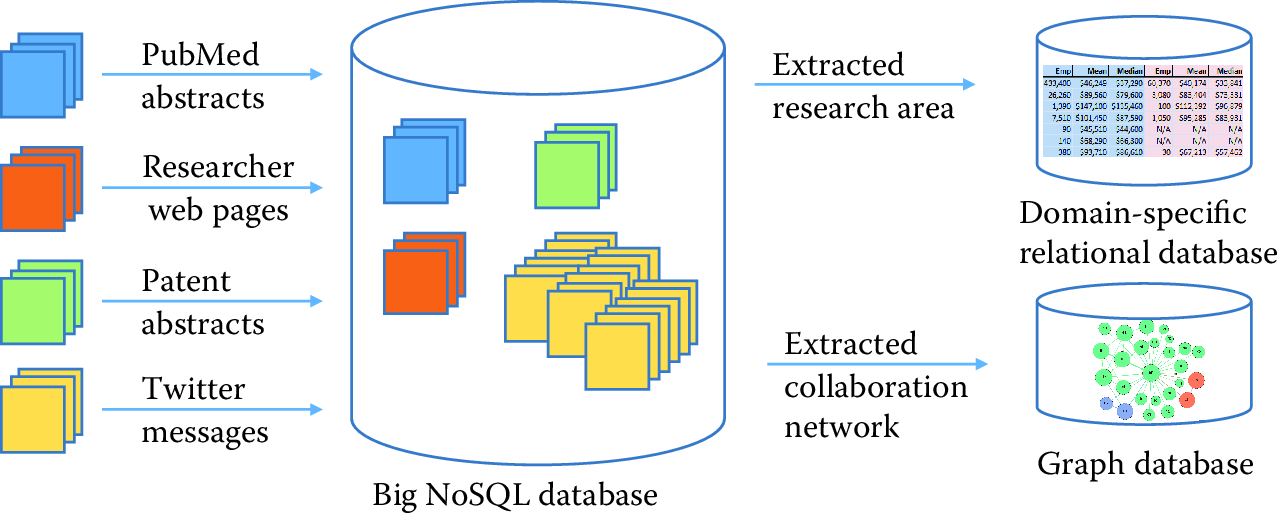
\includegraphics[width=0.7\linewidth]{ChapterDB/figures/data-fig2} 

}

\caption{A research project may use a NoSQL database to accumulate large amounts of data from many different sources, and then extract selected subsets to a relational or other database for more structured processing}\label{fig:figdb-dbs}
\end{figure}

\section{Relational DBMSs}\label{relational-dbmss}

We now provide a more detailed description of relational DBMSs.
Relational DBMSs implement the relational data model, in which data are
represented as sets of records organized in tables. This model is
particularly well suited for the structured, regular data with which we
frequently deal in the social sciences; we discuss in
Section~\protect\hyperlink{sec:db:nosql}{4.5} alternative data models,
such as those used in NoSQL databases.

We use the data shown in Figure~\ref{fig:figdb-1} to introduce key
concepts. These two CSV format files describe grants made by the US
National Science Foundation (NSF). One file contains information about
grants, the other information about investigators. How should you
proceed to manipulate and analyze these data?

\begin{figure}

{\centering 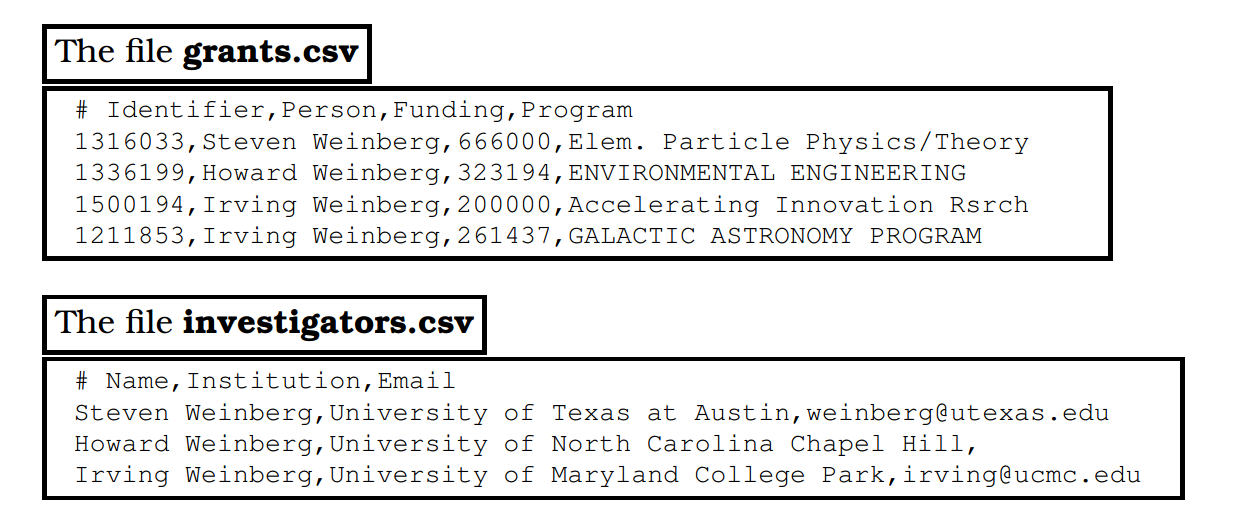
\includegraphics[width=0.7\linewidth]{ChapterDB/figures/figdb-1} 

}

\caption{CSV files representing grants and investigators. Each line in the first table specifies a grant number, investigator name, total funding amount, and NSF program name; each line in the second gives an investigator name, institution name, and investigator email address}\label{fig:figdb-1}
\end{figure}

The main concept underlying the relational data model is a \emph{table}
(also referred to as a \emph{relation}): a set of rows (also referred to
as tuples, records, or observations), each with the same columns (also
referred to as fields, attributes or variables). A database consists of
multiple tables. For example, we show in Figure~\ref{fig:figdb-2} how
the data contained in the two CSV files of Figure~\ref{fig:figdb-1} may
be as two tables. The \texttt{Grants} table contains one tuple for each
row in grants.csv, with columns \texttt{GrantID}, \texttt{Person},
\texttt{Funding}, and \texttt{Program}. The table contains one tuple for
each row in investigators.csv, with columns \texttt{ID}, \texttt{Name},
\texttt{Institution}, and \texttt{Email}. The CSV files and tables
contain essentially the same information, albeit with important
differences (the addition of an \texttt{ID} field in the
\texttt{Investigators} table, the substitution of an \texttt{ID} column
for the \texttt{Person} column in the \texttt{Grants} table) that we
will explain below.

The use of the relational data model provides for physical independence:
a given table can be stored in many different ways. SQL queries are
written in terms of the logical representation of tables (i.e., their
schema definition). Consequently, even if the physical organization of
the data changes (e.g., a different layout is used to store the data on
disk, or a new index is created to speed up access for some queries),
the queries need not change. Another advantage of the relational data
model is that, since a table is a \emph{set}, in a mathematical sense,
simple and intuitive set operations (e.g., union, intersection) can be
used to manipulate the data, as we discuss below. We can easily, for
example, determine the intersection of two relations (e.g., grants that
are awarded to a specific institution), as we describe in the following.
The database further ensures that the data comply with the model (e.g.,
data types, key uniqueness, entity relationships), essentially providing
core quality assurance.

\begin{figure}

{\centering 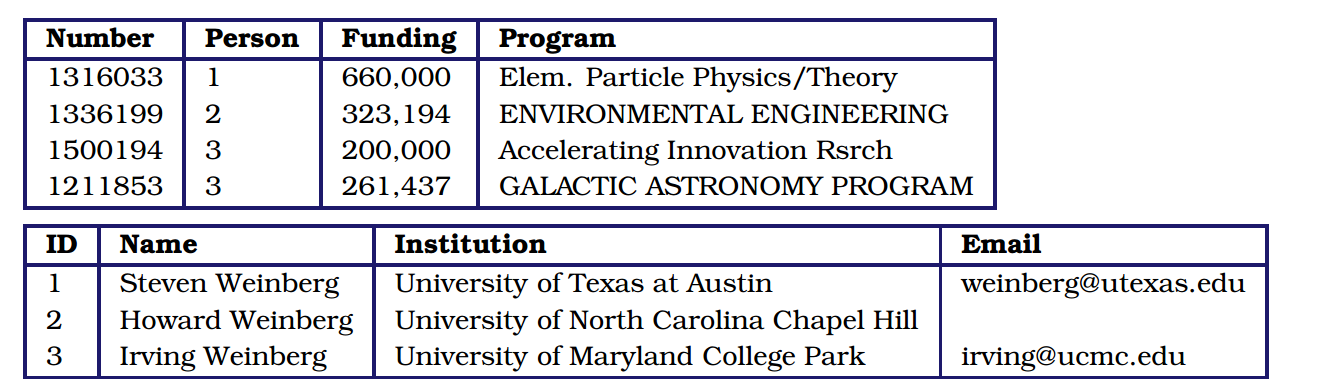
\includegraphics[width=0.7\linewidth]{ChapterDB/figures/figdb-2} 

}

\caption{Relational tables `Grants` and `Investigators` corresponding to the grants.csv and investigators.csv data in Figure 4.2, respectively. The only differences are the representation in a tabular form, the introduction of a unique numerical investigator identifier (`ID`) in the `Investigators` table, and the substitution of that identifier for the investigator name in the `Grants` table}\label{fig:figdb-2}
\end{figure}

\subsection{Structured Query Language
(SQL)}\label{structured-query-language-sql}

We use query languages to manipulate data in a database (e.g., to add,
update, or delete data elements) and to retrieve (raw and aggregated)
data from a database (e.g., data elements that certain properties).
Relational DBMSs support SQL, a simple, powerful query language with a
strong formal foundation based on logic, a foundation that allows
relational DBMSs to perform a wide variety of sophisticated
optimizations. SQL is used for three main purposes:

\begin{itemize}
\item
  \textbf{Data definition}: e.g., creation of new tables,
\item
  \textbf{Data manipulation}: queries and updates,
\item
  \textbf{Control}: creation of assertions to protect data integrity.
\end{itemize}

We introduce each of these features in the following, although not in
that order, and certainly not completely. Our goal here is to give
enough information to provide the reader with insights into how
relational databases work and what they do well; an in-depth SQL
tutorial is beyond the scope of this book but is something we highly
recommend readers seek elsewhere.

\hypertarget{sec:db:sql}{\subsection{Manipulating and querying
data}\label{sec:db:sql}}

SQL and other query languages used in DBMSs support the concise,
declarative specification of complex queries. Because we are eager to
show you something immediately useful, we cover these features first,
before talking about how to define data models.

\begin{center}\rule{0.5\linewidth}{\linethickness}\end{center}

\textbf{Example: Identifying grants of more than \$200,000} Here is an
SQL query to identify all grants with total funding of at most
\$200,000:

\begin{Shaded}
\begin{Highlighting}[]
\KeywordTok{select}\NormalTok{ * }\KeywordTok{from}\NormalTok{ Grants}
\KeywordTok{where}\NormalTok{ Funding <= }\DecValTok{200}\NormalTok{,}\DecValTok{000}\NormalTok{;}
\end{Highlighting}
\end{Shaded}

Notice SQL's declarative nature: this query can be read almost as the
English language statement, ``select all rows from the \texttt{Grants}
table for which the \texttt{Funding} column has value less than or equal
200,000.'' This query is evaluated as follows:

\begin{enumerate}
\def\labelenumi{\arabic{enumi}.}
\item
  The input table specified by the \texttt{from} clause,
  \texttt{Grants}, is selected.
\item
  The condition in the \texttt{where} clause,
  \texttt{Funding\ \textless{}=\ 200,000}, is checked against all rows
  in the input table to identify those rows that match.
\item
  The \texttt{select} clause specifies which columns to keep from the
  matching rows, that is, which columns make the schema of the output
  table. (The ``*'' indicates that all columns should be kept.)
\end{enumerate}

The answer, given the data in Figure~\ref{fig:figdb-2}, is the following
single-row table. (The fact that an SQL query returns a table is
important when it comes to creating more complex queries: the result of
a query can be stored into the database as a new table, or passed to
another query as input.)

\begin{longtable}[]{@{}llll@{}}
\toprule
\textbf{Number} & \textbf{Person} & \textbf{Funding} &
\textbf{Program}\tabularnewline
\midrule
\endhead
1500194 & 3 & 200,000 & Accelerating Innovation Rsrch\tabularnewline
\bottomrule
\end{longtable}

\begin{center}\rule{0.5\linewidth}{\linethickness}\end{center}

DBMSs automatically optimize declarative queries such as the example
that we just presented, translating them into a set of low-level data
manipulations (an imperative \emph{query plan}) that can be evaluated
efficiently. This feature allows users to write queries without having
to worry too much about performance issues---the database does the
worrying for you. For example, a DBMS need not consider every row in the
\texttt{Grants} table in order to identify those with funding less than
\$200,000, a strategy that would be slow if the \texttt{Grants} table
were large: it can instead use an index to retrieve the relevant records
much more quickly. We discuss indices in more detail in
Section~\protect\hyperlink{sec:db:index}{4.3.6}.

The querying component of SQL supports a wide variety of manipulations
on tables, whether referred to explicitly by a table name (as in the
example just shown) or constructed by another query. We just saw how to
use the \texttt{select} operator to both pick certain rows (what is
termed \emph{selection}) and certain columns (what is called
\emph{projection}) from a table.

\begin{center}\rule{0.5\linewidth}{\linethickness}\end{center}

\textbf{Example: Finding grants awarded to an investigator}

We want to find all grants awarded to the investigator with name
``Irving Weinberg.'' The information required to answer this question is
distributed over two tables, \texttt{Grants} and \texttt{Investigators},
and so we \emph{join} the two tables to combine tuples from both:

\begin{Shaded}
\begin{Highlighting}[]
\KeywordTok{select} \DataTypeTok{Number}\NormalTok{, Name, Funding, Program}
\KeywordTok{from}\NormalTok{ Grants, Investigators}
\KeywordTok{where}\NormalTok{ Grants.Person = Investigators.ID}
\KeywordTok{and}\NormalTok{ Name = }\OtherTok{"Irving Weinberg"}\NormalTok{;}
\end{Highlighting}
\end{Shaded}

This query combines tuples from the \texttt{Grants} and
\texttt{Investigators} tables for which the \texttt{Person} and
\texttt{ID} fields match. It is evaluated in a similar fashion to the
query presented above, except for the \texttt{from} clause: when
multiple tables are listed, as here, the conditions in the
\texttt{where} clause are checked for all different combinations of
tuples from the tables defined in the \texttt{from} clause (i.e., the
cartesian product of these tables)---in this case, a total of
\(3\times 4 = 12\) combinations. We thus determine that Irving Weinberg
has two grants. The query further selects the \texttt{Number},
\texttt{Name}, \texttt{Funding}, and \texttt{Program} fields from the
result, giving the following:

\begin{longtable}[]{@{}llll@{}}
\toprule
\textbf{Number} & \textbf{Person} & \textbf{Funding} &
\textbf{Program}\tabularnewline
\midrule
\endhead
1500194 & Irving Weinberg & 200,000 & Accelerating Innovation
Rsrch\tabularnewline
1211853 & Irving Weinberg & 261,437 & GALACTIC ASTRONOMY
PROGRAM\tabularnewline
\bottomrule
\end{longtable}

This ability to join two tables in a query is one example of how SQL
permits concise specifications of complex computations. This joining of
tables via a cartesian product operation is formally called a
\emph{cross join}. Other types of join are also supported. We describe
one such, the \emph{inner join}, in
Section~\protect\hyperlink{sec:db:spatial}{4.6}.

\begin{center}\rule{0.5\linewidth}{\linethickness}\end{center}

SQL aggregate functions allow for the computation of aggregate
statistics over tables. For example, we can use the following query to
determine the total number of grants and their total and average funding
levels:

\begin{Shaded}
\begin{Highlighting}[]
\KeywordTok{select} \FunctionTok{count}\NormalTok{(*) }\KeywordTok{as} \StringTok{'Number'}\NormalTok{, }\FunctionTok{sum}\NormalTok{(Funding) }\KeywordTok{as} \StringTok{'Total'}\NormalTok{,}
       \FunctionTok{avg}\NormalTok{(Funding) }\KeywordTok{as} \StringTok{'Average'}
\KeywordTok{from}\NormalTok{ Grants;}
\end{Highlighting}
\end{Shaded}

This yields the following:

\begin{longtable}[]{@{}lll@{}}
\toprule
\textbf{Number} & \textbf{Total} & \textbf{Average}\tabularnewline
\midrule
\endhead
4 & 1444631 & 361158\tabularnewline
\bottomrule
\end{longtable}

The \texttt{group\ by} operator can be used in conjunction with the
aggregate functions to group the result set by one or more columns. For
example, we can use the following query to create a table with three
columns: investigator name, the number of grants associated with the
investigator, and the aggregate funding:

\begin{Shaded}
\begin{Highlighting}[]
\KeywordTok{select}\NormalTok{ Name, }\FunctionTok{count}\NormalTok{(*) }\KeywordTok{as} \StringTok{'Number'}\NormalTok{,}
       \FunctionTok{avg}\NormalTok{(Funding) }\KeywordTok{as} \StringTok{'Average funding'}
\KeywordTok{from}\NormalTok{ Grants, Investigators}
\KeywordTok{where}\NormalTok{ Grants.Person = Investigators.ID}
\KeywordTok{group} \KeywordTok{by}\NormalTok{ Name;}
\end{Highlighting}
\end{Shaded}

We obtain the following:

\begin{longtable}[]{@{}lll@{}}
\toprule
\textbf{Name} & \textbf{Number} & \textbf{Average
Funding}\tabularnewline
\midrule
\endhead
Steven Weinberg & 1 & 666000\tabularnewline
Howard Weinberg & 1 & 323194\tabularnewline
Irving Weinberg & 2 & 230719\tabularnewline
\bottomrule
\end{longtable}

\hypertarget{sec:db:schema}{\subsection{Schema design and
definition}\label{sec:db:schema}}

We have seen that a relational database comprises a set of tables. The
task of specifying the structure of the data to be stored in a database
is called \emph{logical design}. This task may be performed by a
database administrator, in the case of a database to be shared by many
people, or directly by users, if they are creating databases themselves.
More specifically, the logical design process involves defining a
\emph{schema}. A schema comprises a set of tables (including, for each
table, its columns and their types), their relationships, and integrity
constraints.

The first step in the logical design process is to identify the entities
that need to be modeled. In our example, we identified two important
classes of entity: ``grants'' and ``investigators.'' We thus define a
table for each; each row in these two tables will correspond to a unique
grant or investigator, respectively. (In a more complete and realistic
design, we would likely also identify other entities, such as
institutions and research products.) During this step, we will often
find ourselves breaking information up into multiple tables, so as to
avoid duplicating information.

For example, imagine that we were provided grant information in the form
of one CSV file rather than two, with each line providing a grant
number, investigator, funding, program, institution, and email. In this
file, the name, institution, and email address for Irving Weinberg would
then appear twice, as he has two grants, which can lead to errors when
updating values and make it difficult to represent certain information.
(For example, if we want to add an investigator who does not yet have a
grant, we will need to create a tuple (row) with empty slots for all
columns (variables) associated with grants.) Thus we would want to break
up the single big table into the two tables that we defined here. This
breaking up of information across different tables to avoid repetition
of information is referred to as \textbf{normalization}.\footnote{Normalization
  involves organizing columns and tables of a relational database to
  minimize data redundancy.}\footnote{Normalization can be done in
  statistical packages as well. For example, as noted above, PSID splits
  its data into different files linked through ID variables. The
  difference here is that the DBMS makes creating, navigating, and
  querying the resulting data particularly easy.}

The second step in the design process is to define the columns that are
to be associated with each entity. For each table, we define a set of
columns. For example, given the data in Figure~\ref{fig:figdb-1}, those
columns will likely include, for a grant, an award identifier, title,
investigator, and award amount; for an investigator, a name, university,
and email address. In general, we will want to ensure that each row in
our table has a key: a set of columns that uniquely identifies that row.
In our example tables, grants are uniquely identified by \texttt{Number}
and investigators by \texttt{ID}.

The third step in the design process is to capture relationships between
entities. In our example, we are concerned with just one relationship,
namely that between grants and investigators: each grant has an
investigator. We represent this relationship between tables by
introducing a \texttt{Person} column in the \texttt{Grants} table, as
shown in Figure~\ref{fig:figdb-2}. Note that we do not simply duplicate
the investigator names in the two tables, as was the case in the two CSV
files shown in Figure~\ref{fig:figdb-1}: these names might not be
unique, and the duplication of data across tables can lead to later
inconsistencies if a name is updated in one table but not the other.

The final step in the design process is to represent integrity
constraints (or rules) that must hold for the data. In our example, we
may want to specify that each grant must be awarded to an investigator;
that each value of the grant identifier column must be unique (i.e.,
there cannot be two grants with the same number); and total funding can
never be negative. Such restrictions can be achieved by specifying
appropriate constraints at the time of schema creation, as we show in
Listing 4.1, which contains the code used to create the two tables that
make up our schema.

Listing 4.1 contains four SQL statements. The first two statements,
lines 1 and 2, simply set up our new database. The
\texttt{create\ table} statement in lines 1 and 2 creates our first
table. It specifies the table name (\texttt{Investigators}) and, for
each of the four columns, the column name and its type.\footnote{These
  storage types will be familiar to many of you from statistical
  software packages.} Relational DBMSs offer a rich set of types to
choose from when designing a schema: for example, \texttt{int} or
\texttt{integer} (synonyms); \texttt{real} or \texttt{float}(synonyms);
\texttt{char(n)}, a fixed-length string of \texttt{n} characters; and
\texttt{varchar(n)}, a variable-length string of up to \texttt{n}
characters. Types are important for several reasons. First, they allow
for more efficient encoding of data. For example, the \texttt{Funding}
field in the grants.csv file of Figure~\ref{fig:figdb-1} could be
represented as a string in the \texttt{Grants} table, \texttt{char(15)},
say, to allow for large grants. By representing it as a floating point
number instead (line 15 in Listing 4.1), we reduce the space requirement
per grant to just four bytes. Second, types allow for integrity checks
on data as they are added to the database: for example, that same type
declaration for \texttt{Funding} ensures that only valid numbers will be
entered into the database. Third, types allow for type-specific
operations on data, such as arithmetic operations on numbers (e.g., min,
max, sum).

Other SQL features allow for the specification of additional constraints
on the values that can be placed in the correspondingcolumn. For
example, the \texttt{not\ null} constraints for \texttt{Name} and
\texttt{Institution} (lines 6, 7) indicate that each investigator must
have a name and an institution, respectively. (The lack of such a
constraint on the \texttt{Email} column shows that an investigator need
not have an email address.)

\hypertarget{fig:db:create}{\label{fig:db:create}}
\begin{verbatim}
create database grantdata;
use grantdata;

create table Investigators ( --latexlabel `\label{code:db:1}`
    ID int auto_increment, --latexlabel `\label{code:db:9}`
    Name varchar(100) not null, --latexlabel `\label{code:db:7}`
    Institution varchar(256) not null, --latexlabel `\label{code:db:8}`
    Email varchar(100),
    primary key(ID)
);  --latexlabel `\label{code:db:2}`

create table Grants ( --latexlabel `\label{code:db:10}`
    Number int not null, --latexlabel `\label{code:db:6}`
    Person int not null,
    Funding float unsigned not null, --latexlabel `\label{code:db:5}`
    Program varchar(100),
    primary key(Number)
); --latexlabel `\label{code:db:11}`
\end{verbatim}

Listing 4.1. Code to create the grantdata database and its Investigators
and Grants tables

\subsection{Loading data}\label{loading-data}

So far we have created a database and two tables. To complete our simple
SQL program, we show in Listing 4.2 the two statements that load the
data of Figure~\ref{fig:figdb-1} into our two tables. (Here and
elsewhere in this chapter, we use the MySQL DBMS. The SQL syntax used by
different DBMSs differs in various, mostly minor ways.) Each statement
specifies the name of the file from which data is to be read and the
table into which it is to be loaded. The
\texttt{fields\ terminated\ by\ ","} statement tells SQL that values are
separated by columns, and \texttt{ignore\ 1\ lines} tells SQL to skip
the header. The list of column names is used to specify how values from
the file are to be assigned to columns in the table.

For the \texttt{Investigators} table, the three values in each row of
the investigators.csv file are assigned to the \texttt{Name},
\texttt{Institution}, and \texttt{Email} columns of the corresponding
database row. Importantly, the \texttt{auto\_increment}declaration on
the \texttt{ID} column (line 5 in Listing 4.1) causes values for this
column to be assigned automatically by the DBMS, as rows are created,
starting at \texttt{1}. This feature allows us to assign a unique
integer identifier to each investigator as its data are loaded.

\hypertarget{fig:db:load}{\label{fig:db:load}}
\begin{verbatim}
load data local infile "investigators.csv"
    into table Investigators
    fields terminated by ","
    ignore 1 lines
    (Name, Institution, Email);

load data local infile "grants.csv" into table Grants --latexlabel `\label{code:db:3}`
    fields terminated by ","
    ignore 1 lines
    (Number, @var, Funding, Program)
set Person = (select ID from Investigators --latexlabel `\label{code:db:4a}`
              where Investigators.Name=@var); --latexlabel `\label{code:db:4}`
\end{verbatim}

Listing 4.2. Code to load data into the Investigators and Grants tables

For the \texttt{Grants} table, the \texttt{load\ data} call (lines
7--12) is somewhat more complex. Rather than loading the investigator
name (the second column of each line in our data file, represented here
by the variable \texttt{@var}) directly into the database, we use an SQL
query (the \texttt{select} statement in lines 11--12) to retrieve from
the \texttt{Investigators} table the \texttt{ID} corresponding to that
name. By thus replacing the investigator name with the unique
investigator identifier, we avoid replicating the name across the two
tables.

\subsection{Transactions and crash
recovery}\label{transactions-and-crash-recovery}

A DBMS protects the data that it stores from computer crashes: if your
computer stops running suddenly (e.g., your operating system crashes or
you unplug the power), the contents of your database are not corrupted.
It does so by supporting \emph{transactions}. A transaction is an atomic
sequence of database actions. In general, every SQL statement is
executed as a transaction. You can also specify sets of statements to be
combined into a single transaction, but we do not cover that capability
here. The DBMS ensures that each transaction is executed completely even
in the case of failure or error: if the transaction succeeds, the
results of all operations are recorded permanently (``persisted'') in
the database, and if it fails, all operations are ``rolled back'' and no
changes are committed. For example, suppose we ran the following SQL
statement to convert the funding amounts in the table from dollars to
euros, by scaling each number by 0.9. The \texttt{update} statement
specifies the table to be updated and the operation to be performed,
which in this case is to update the \texttt{Funding} column of each row.
The DBMS will ensure that either no rows are altered or all are altered.

\begin{Shaded}
\begin{Highlighting}[]
\KeywordTok{update}\NormalTok{ Grants }\KeywordTok{set}\NormalTok{ Grants.Funding = Grants.Funding*}\FloatTok{0.9}\NormalTok{;}
\end{Highlighting}
\end{Shaded}

Transactions are also key to supporting multi-user access. The
\emph{concurrency control} mechanisms in a DBMS allow multiple users to
operate on a database concurrently, as if they were the only users of
the system: transactions from multiple users can be interleaved to
ensure fast response times, while the DBMS ensures that the database
remains consistent. While entire books could be (and have been) written
on concurrency in databases, the key point is that read operations can
proceed concurrently, while update operations are typically serialized.

\hypertarget{sec:db:index}{\subsection{Database
optimizations}\label{sec:db:index}}

A relational DBMS applies query planning and optimization methods with
the goal of evaluating queries as efficiently as possible. For example,
if a query asks for rows that fit two conditions, one cheap to evaluate
and one expensive, a relational DBMS may filter first on the basis of
the first condition, and then apply the second conditions only to the
rows identified by that first filter. These sorts of optimization are
what distinguish SQL from other programming languages, as they allow the
user to write queries declaratively and rely on the DBMS to come up with
an efficient execution strategy.

Nevertheless, the user can help the DBMS to improve performance. The
single most powerful performance improvement tool is the index, an
internal data structure that the DBMS maintains to speed up queries.
While various types of indices can be created, with different
characteristics, the basic idea is simple. Consider the column in our
table. Assume that there are \(N\) rows in the table. In the absence of
an index, a query that refers to a column value (e.g., ) would require a
linear scan of the table, taking on average \(N/2\) comparisons and in
the worst case \(N\) comparisons. A binary tree index allows the desired
value to be found with just \(\log_2 N\) comparisons.

\begin{center}\rule{0.5\linewidth}{\linethickness}\end{center}

\textbf{Example: Using indices to improve database performance}

Consider the following query:

\begin{Shaded}
\begin{Highlighting}[]
\KeywordTok{select} \KeywordTok{ID}\NormalTok{, Name, }\FunctionTok{sum}\NormalTok{(Funding) }\KeywordTok{as}\NormalTok{ TotalFunding}
  \KeywordTok{from}\NormalTok{ Grants, Investigators}
    \KeywordTok{where}\NormalTok{ Investigators.ID=Grants.Person}
  \KeywordTok{group} \KeywordTok{by} \KeywordTok{ID}\NormalTok{;}
\end{Highlighting}
\end{Shaded}

This query joins our two tables to link investigators with the grants
that they hold, groups grants by investigator (using
\texttt{group\ by}), and finally sums the funding associated with the
grants held by each investigator. The result is the following:

\begin{longtable}[]{@{}lll@{}}
\toprule
\textbf{ID} & \textbf{Name} & \textbf{TotalFunding}\tabularnewline
\midrule
\endhead
1 & Steven Weinberg & 666000\tabularnewline
2 & Howard Weinberg & 323194\tabularnewline
3 & Irving Weinberg & 230719\tabularnewline
\bottomrule
\end{longtable}

In the absence of indices, the DBMS must compare each row in
\texttt{Investigators} with each row in \texttt{Grants}, checking for
each pair whether \texttt{Investigators.ID\ =\ Grants.Person} holds. As
the two tables in our sample database have only three and four rows,
respectively, the total number of comparisons is only \(3\times 4=12\).
But if we had, say, 1 million investigators and 1 million grants, then
the DBMS would have to perform 1 trillion comparisons, which would take
a long time. (More importantly in many cases, it would have to perform a
large number of disk I/O operations if the tables did not fit in
memory.) An index on the \texttt{ID} column of the
\texttt{Investigators} table reduces the number of operations
dramatically, as the DBMS can then take each of the 1 million rows in
the \texttt{Grants} table and, for each row, identify the matching
row(s) in \texttt{Investigators} via an index lookup rather than a
linear scan.

In our example table, the \texttt{ID} column has been specified to be a
\texttt{primary\ key}, and thus an index is created for it
automatically. If it were not, we could easily create the desired index
as follows:

\begin{Shaded}
\begin{Highlighting}[]
\KeywordTok{alter} \KeywordTok{table}\NormalTok{ Investigators }\KeywordTok{add} \KeywordTok{index}\NormalTok{(}\KeywordTok{ID}\NormalTok{);}
\end{Highlighting}
\end{Shaded}

It can be difficult for the user to determine when an index is required.
A good rule of thumb is to create an index for any column that is
queried often, that is, appears on the right-hand side of a
\texttt{where} statement. However, the presence of indices makes updates
more expensive, as every change to a column value requires that the
index be rebuilt to reflect the change. Thus, if your data are highly
dynamic, you should carefully select which indices to create. (For bulk
load operations, a common practice is to drop indices prior to the data
import, and re-create them once the load is completed.) Also, indices
take disk space, so you need to consider the tradeoff between query
efficiency and resources.

The \texttt{explain} command can be useful for determining when indices
are required. For example, we show in the following some of the output
produced when we apply \texttt{explain} to our query. (For this example,
we have expanded the two tables to 1,000 rows each, as our original
tables are too small for MySQL to consider the use of indices.) The
output provides useful information such as the key(s) that could be
used, if indices exist (\texttt{Person} in the \texttt{Grants} table,
and the primary key, \texttt{ID}, for the \texttt{Investigators} table);
the key(s) that are actually used (the primary key, \texttt{ID}, in the
\texttt{Investigators} table); the column(s) that are compared to the
index (\texttt{Investigators.ID} is compared with
\texttt{Grants.Person}); and the number of rows that must be considered
(each of the 1,000 rows in \texttt{Grants} is compared with one row in
\texttt{Investigators}, for a total of 1,000 comparisons).

\begin{Shaded}
\begin{Highlighting}[]
\NormalTok{mysql> }\KeywordTok{explain} \KeywordTok{select} \KeywordTok{ID}\NormalTok{, Name, }\FunctionTok{sum}\NormalTok{(Funding) }\KeywordTok{as}\NormalTok{ TotalFunding}
       \KeywordTok{from}\NormalTok{ Grants, Investigators}
       \KeywordTok{where}\NormalTok{ Investigators.ID=Grants.Person }\KeywordTok{group} \KeywordTok{by} \KeywordTok{ID}\NormalTok{;}

\NormalTok{+}\CommentTok{---------------+---------------+---------+---------------+------+}
\NormalTok{| }\KeywordTok{table}\NormalTok{         | possible_keys | }\KeywordTok{key}\NormalTok{     | }\FunctionTok{ref}\NormalTok{           | }\KeywordTok{rows}\NormalTok{ |}
\NormalTok{+}\CommentTok{---------------+---------------+---------+---------------+------+}
\NormalTok{| Grants        | Person        | }\KeywordTok{NULL}\NormalTok{    | }\KeywordTok{NULL}\NormalTok{          | }\DecValTok{1000}\NormalTok{ |}
\NormalTok{| Investigators | }\KeywordTok{PRIMARY}\NormalTok{       | }\KeywordTok{PRIMARY}\NormalTok{ | Grants.Person |    }\DecValTok{1}\NormalTok{ |}
\NormalTok{+}\CommentTok{---------------+---------------+---------+---------------+------+}
\end{Highlighting}
\end{Shaded}

Contrast this output with the output obtained for equivalent tables in
which is not a primary key. In this case, no keys are used and thus
\(1{,}000\times 1{,}000=1{,}000{,}000\) comparisons and the associated
disk reads must be performed.

\begin{Shaded}
\begin{Highlighting}[]
\NormalTok{+}\CommentTok{---------------+---------------+------+------+------+}
\NormalTok{| }\KeywordTok{table}\NormalTok{         | possible_keys | }\KeywordTok{key}\NormalTok{  | }\FunctionTok{ref}\NormalTok{  | }\KeywordTok{rows}\NormalTok{ |}
\NormalTok{+}\CommentTok{---------------+---------------+------+------+------+}
\NormalTok{| Grants        | Person        | }\KeywordTok{NULL}\NormalTok{ | }\KeywordTok{NULL}\NormalTok{ | }\DecValTok{1000}\NormalTok{ |}
\NormalTok{| Investigators | }\KeywordTok{ID}\NormalTok{            | }\KeywordTok{NULL}\NormalTok{ | }\KeywordTok{NULL}\NormalTok{ | }\DecValTok{1000}\NormalTok{ |}
\NormalTok{+}\CommentTok{---------------+---------------+------+------+------+}
\end{Highlighting}
\end{Shaded}

\begin{center}\rule{0.5\linewidth}{\linethickness}\end{center}

A second way in which the user can contribute to performance improvement
is by using appropriate table definitions and data types. Most DBMSs
store data on disk. Data must be read from disk into memory before it
can be manipulated. Memory accesses are fast, but loading data into
memory is expensive: accesses to main memory can be a million times
faster than accesses to disk. Therefore, to ensure queries are
efficient, it is important to minimize the number of disk accesses. A
relational DBMS automatically optimizes queries: based on how the data
are stored, it transforms a SQL query into a query plan that can be
executed efficiently, and chooses an execution strategy that minimizes
disk accesses. But users can contribute to making queries efficient. As
discussed above, the choice of types made when defining schemas can make
a big difference. As a rule of thumb, only use as much space as needed
for your data: the smaller your records, the more records can be
transferred to main memory using a single disk access. The design of
relational tables is also important. If you put all columns in a single
table (do not normalize), more data will come into memory than is
required.

\subsection{Caveats and challenges}\label{caveats-and-challenges}

It is important to keep the following caveats and challenges in mind
when using SQL technology with social science data.

\textbf{Data cleaning}

Data created outside an SQL database, such as data in files, are not
always subject to strict constraints: data types may not be correct or
consistent (e.g., numeric data stored as text) and consistency or
integrity may not be enforced (e.g., absence of primary keys, missing
foreign keys). Indeed, as the reader probably knows well from
experience, data are rarely perfect. As a result, the data may fail to
comply with strict SQL schema requirements and fail to load, in which
case either data must be cleaned before or during loading, or the SQL
schema must be relaxed.

\textbf{Missing values}

Care must be taken when loading data in which some values may be missing
or blank. SQL engines represent and refer to a missing or blank value as
the built-in constant \texttt{null}. Counterintuitively, when loading
data from text files (e.g., CSV), many SQL engines require that missing
values be represented explicitly by the term \texttt{null}; if a data
value is simply omitted, it may fail to load or be incorrectly
represented, for example as zero or the empty string (\texttt{"\ "})
instead of \texttt{null}. Thus, for example, the second row in the
investigators.csv file of Figure~\ref{fig:figdb-1}:

\texttt{Howard\ Weinberg,University\ of\ North\ Carolina\ Chapel\ Hill,}

may need to be rewritten as:

\texttt{Howard\ Weinberg,University\ of\ North\ Carolina\ Chapel\ Hill,null}

\textbf{Metadata for categorical variables}

SQL engines are metadata poor: they do not allow extra information to be
stored about a variable (field) beyond its base name and type
(\texttt{int}, \texttt{char}, etc., as introduced in
Section~\protect\hyperlink{sec:db:schema}{4.3.3}). They cannot, for
example, record directly the fact that the column \texttt{class} can
only take one of three values, \texttt{animal}, \texttt{vegetable}, or
\texttt{mineral}, or what these values mean. Common practice is thus to
store information about possible values in another table (commonly
referred to as a \emph{dimension table}) that can be used as a lookup
and constraint, as in the following:

Table \textbf{class\_values}

\begin{longtable}[]{@{}ll@{}}
\toprule
\textbf{Value} & \textbf{Description}\tabularnewline
\midrule
\endhead
\texttt{animal} & Is alive\tabularnewline
\texttt{vegetable} & Grows\tabularnewline
\texttt{mineral} & Isn't alive and doesn't grow\tabularnewline
\bottomrule
\end{longtable}

A related concept is that a column or list of columns may be declared
\texttt{primary\ key} or \texttt{unique}. Either says that no two tuples
of the table may agree in all the column(s) on the list. There can be
only one \texttt{primary\ key} for a table, but several \texttt{unique}
columns. No column of a \texttt{primary\ key} can ever be \texttt{null}
in any tuple. But columns declared \texttt{unique} may have
\texttt{null}s, and there may be several tuples with \texttt{null}.

\section{Linking DBMSs and other
tools}\label{linking-dbmss-and-other-tools}

Query languages such as SQL are not general-purpose programming
languages; they support easy, efficient access to large data sets, but
are not intended to be used for complex calculations. When complex
computations are required, one can embed query language statements into
a programming language or statistical package. For example, we might
want to calculate the interquartile range of funding for all grants.
While this calculation can be accomplished in SQL, the resulting SQL
code will be complicated. Languages like Python make such statistical
calculations straightforward, so it is natural to write a Python (or R,
SAS, Stata, etc.) program that connects to the DBMS that contains our
data, fetches the required data from the DBMS, and then calculates the
interquartile range of those data. The program can then, if desired,
store the result of this calculation back into the database.

Many relational DBMSs also have built-in analytical functions or often
now embed the R engine, providing significant in-database statistical
and analytical capabilities and alleviating the need for external
processing.

\begin{Shaded}
\begin{Highlighting}[]
\NormalTok{from mysql.connector import MySQLConnection, Error}
\NormalTok{from python_mysql_dbconfig import read_db_config}

\NormalTok{def }\KeywordTok{retrieve_and_analyze_data}\NormalTok{()}\OperatorTok{:}
\StringTok{    }\NormalTok{try}\OperatorTok{:}
\StringTok{        }\CommentTok{# Open connection to the MySQL database}
\StringTok{        }\NormalTok{dbconfig =}\StringTok{ }\KeywordTok{read_db_config}\NormalTok{() }\OperatorTok{--}\NormalTok{latexlabel }\StringTok{`}\DataTypeTok{\textbackslash{}label\{code:db:a\}}\StringTok{`}
\NormalTok{        conn =}\StringTok{ }\KeywordTok{MySQLConnection}\NormalTok{(}\OperatorTok{**}\NormalTok{dbconfig)}
\NormalTok{        cursor =}\StringTok{ }\KeywordTok{conn.cursor}\NormalTok{() }\OperatorTok{--}\NormalTok{latexlabel }\StringTok{`}\DataTypeTok{\textbackslash{}label\{code:db:b\}}\StringTok{`}
        \CommentTok{# Transmit the SQL query to the database}
        \KeywordTok{cursor.execute}\NormalTok{(}\StringTok{'select Funding from Grants;'}\NormalTok{) }\OperatorTok{--}\NormalTok{latexlabel }\StringTok{`}\DataTypeTok{\textbackslash{}label\{code:db:c\}}\StringTok{`}
        \CommentTok{# Fetch all rows of the query response}
\NormalTok{        rows =}\StringTok{ }\NormalTok{[row }\ControlFlowTok{for}\NormalTok{ row }\ControlFlowTok{in} \KeywordTok{cur.fetchall}\NormalTok{()] }\OperatorTok{--}\NormalTok{latexlabel }\StringTok{`}\DataTypeTok{\textbackslash{}label\{code:db:d\}}\StringTok{`}
        \KeywordTok{calculate_inter_quartile_range}\NormalTok{(rows) }\OperatorTok{--}\NormalTok{latexlabel }\StringTok{`}\DataTypeTok{\textbackslash{}label\{code:db:e\}}\StringTok{`}
\NormalTok{    except Error as e}\OperatorTok{:}
\StringTok{        }\KeywordTok{print}\NormalTok{(e)}
\NormalTok{    finally}\OperatorTok{:}
\StringTok{        }\KeywordTok{cursor.close}\NormalTok{()}
        \KeywordTok{conn.close}\NormalTok{()}

\ControlFlowTok{if}\NormalTok{ __name__ }\OperatorTok{==}\StringTok{ '__main__'}\OperatorTok{:}
\StringTok{    }\KeywordTok{retrieve_and_analyze_data}\NormalTok{()}
\end{Highlighting}
\end{Shaded}

Listing 4.3. Embedding SQL in Python

\begin{center}\rule{0.5\linewidth}{\linethickness}\end{center}

\textbf{Example: Embedding database queries in Python}

The Python script in Listing 4.3 shows how this embedding of database
queries in Python is done. This script establishes a connection to the
database transmits the desired SQL query to the database (line 7--9),
retrieves the query results into a Python array (line 11), and calls a
Python procedure (not given) to perform the desired computation (line
14). A similar program could be used to load the results of a Python (or
R, SAS, Stata, etc.) computation into a database.

\begin{center}\rule{0.5\linewidth}{\linethickness}\end{center}

\begin{center}\rule{0.5\linewidth}{\linethickness}\end{center}

\textbf{Example: Loading other structured data}

We saw in Listing 4.2 how to load data from CSV files into SQL tables.
Data in other formats, such as the commonly used JSON, can also be
loaded into a relational DBMS. Consider, for example, the following JSON
format data, a simplified version of data shown in Chapter
\protect\hyperlink{chap:web}{Working with Web Data and APIs}.

\pagebreak

\begin{Shaded}
\begin{Highlighting}[]
\NormalTok{[}
\NormalTok{  \{}
\NormalTok{    institute }\OperatorTok{:}\StringTok{ }\NormalTok{Janelia Campus,}
\NormalTok{    name }\OperatorTok{:}\StringTok{ }\NormalTok{Laurence Abbott,}
\NormalTok{    role }\OperatorTok{:}\StringTok{ }\NormalTok{Senior Fellow,}
\NormalTok{    state }\OperatorTok{:}\StringTok{ }\NormalTok{VA,}
\NormalTok{    town }\OperatorTok{:}\StringTok{ }\NormalTok{Ashburn}
\NormalTok{  \},}
\NormalTok{  \{}
\NormalTok{    institute }\OperatorTok{:}\StringTok{ }\NormalTok{Jackson Lab,}
\NormalTok{    name }\OperatorTok{:}\StringTok{ }\NormalTok{Susan Ackerman,}
\NormalTok{    role }\OperatorTok{:}\StringTok{ }\NormalTok{Investigator,}
\NormalTok{    state }\OperatorTok{:}\StringTok{ }\NormalTok{ME,}
\NormalTok{    town }\OperatorTok{:}\StringTok{ }\NormalTok{Bar Harbor}
\NormalTok{  \}}
\NormalTok{]}
\end{Highlighting}
\end{Shaded}

While some relational DBMSs provide built-in support for JSON objects,
we assume here that we want to convert these data into normal SQL
tables. Using one of the many utilities for converting JSON into CSV, we
can construct the following CSV file, which we can load into an SQL
table using the method shown earlier.

\begin{verbatim}
institute,name,role,state,town
Janelia Campus,Laurence Abbott,Senior Fellow,VA,Ashburn
Jackson Lab,Susan Ackerman,Investigator,ME,Bar Harbor
\end{verbatim}

But into what table? The two records each combine information about a
person with information about an institute. Following the schema design
rules given in Section~\protect\hyperlink{sec:db:schema}{4.3.3}, we
should \emph{normalize} the data by reorganizing them into two tables,
one describing people and one describing institutes. Similar problems
arise when JSON documents contain nested structures. For example,
consider the following alternative JSON representation of the data
above. Here, the need for normalization is yet more apparent.

\begin{Shaded}
\begin{Highlighting}[]
\NormalTok{[}
\NormalTok{  \{}
\NormalTok{    name }\OperatorTok{:}\StringTok{ }\NormalTok{Laurence Abbott,}
\NormalTok{    role }\OperatorTok{:}\StringTok{ }\NormalTok{Senior Fellow,}
\NormalTok{    employer }\OperatorTok{:}\StringTok{ }\NormalTok{\{ institute }\OperatorTok{:}\StringTok{ }\NormalTok{Janelia Campus,}
\NormalTok{                 state }\OperatorTok{:}\StringTok{ }\NormalTok{VA,}
\NormalTok{                 town }\OperatorTok{:}\StringTok{ }\NormalTok{Ashburn\}}
\NormalTok{  \},}
\NormalTok{  \{}
\NormalTok{    name }\OperatorTok{:}\StringTok{ }\NormalTok{Susan Ackerman,}
\NormalTok{    role }\OperatorTok{:}\StringTok{ }\NormalTok{Investigator,}
\NormalTok{    employer}\OperatorTok{:}\StringTok{ }\NormalTok{\{ institute }\OperatorTok{:}\StringTok{ }\NormalTok{Jackson Lab,}
\NormalTok{                state }\OperatorTok{:}\StringTok{ }\NormalTok{ME,}
\NormalTok{                town }\OperatorTok{:}\StringTok{ }\NormalTok{Bar Harbor\}}
\NormalTok{  \}}
\NormalTok{]}
\end{Highlighting}
\end{Shaded}

Thus, the loading of JSON data into a relational database usually
requires both work on schema design
(Section~\protect\hyperlink{sec:db:schema}{4.3.3}) and data preparation.

\begin{center}\rule{0.5\linewidth}{\linethickness}\end{center}

\hypertarget{sec:db:nosql}{\section{NoSQL
databases}\label{sec:db:nosql}}

While relational DBMSs have dominated the database world for several
decades, other database technologies exist and indeed have popular for
various classes of applications in recent years. As we will see, these
alternative technologies have typically been motivated by a desire to
scale the quantities of data and/or number of users that can be
supported, and/or to support specialized data types (e.g., unstructured
data, graphs). Here we review some of these alternatives and the factors
that may motivate their use.

\subsection{Challenges of scale: The CAP
theorem}\label{challenges-of-scale-the-cap-theorem}

For many years, the big relational database vendors (Oracle, IBM,
Sybase, and to a lesser extent Microsoft) have been the mainstay of how
data were stored. During the Internet boom, startups looking for
low-cost alternatives to commercial relational DBMSs turned to MySQL and
PostgreSQL. However, these systems proved inadequate for big sites as
they could not cope well with large traffic spikes, for example when
many customers all suddenly wanted to order the same item. That is, they
did not \emph{scale}.

An obvious solution to scaling databases is to partition and/or
replicate data across multiple computers, for example by distributing
different tables, or different rows from the same table, over multiple
computers. However, partitioning and replication also introduce
challenges, as we now explain. Let us first define some terms. In a
system that comprises multiple computers:

\begin{itemize}
\item
  \textbf{Consistency} indicates that all computers see the same data at
  the same time.
\item
  \textbf{Availability} indicates that every request receives a response
  about whether it succeeded or failed.
\item
  \textbf{Partition tolerance} indicates that the system continues to
  operate even if a network failure prevents computers from
  communicating.
\end{itemize}

An important result in distributed systems (the so-called ``CAP
theorem'' (Brewer \protect\hyperlink{ref-brewer2012cap}{2012})) observes
that it is not possible to create a distributed system with all three
properties. This situation creates a challenge with large transactional
data sets. Partitioning is needed in order to achieve high performance,
but as the number of computers grows, so too does the likelihood of
network disruption among pair(s) of computers. As strict consistency
cannot be achieved at the same time as availability and partition
tolerance, the DBMS designer must choose between high consistency and
high availability for a particular system.

The right combination of availability and consistency will depend on the
needs of the service. For example, in an e-commerce setting, it makes
sense to choose high availability for a checkout process, in order to
ensure that requests to add items to a shopping cart (a
revenue-producing process) can be honored. Errors can be hidden from the
customer and sorted out later. However, for order submission---when a
customer submits an order---it makes sense to favor consistency because
several services (credit card processing, shipping and handling,
reporting) need to access the data simultaneously. However, in almost
all cases, availability is chosen over consistency.

\subsection{NoSQL and key--value
stores}\label{nosql-and-keyvalue-stores}

Relational DBMSs were traditionally motivated by the need for
transaction processing and analysis, which led them to put a premium on
consistency and availability. This led the designers of these systems to
provide a set of properties summarized by the acronym ACID (Gray
\protect\hyperlink{ref-gray1981transaction}{1981}; Silberschatz, Korth,
and Sudarshan \protect\hyperlink{ref-silberschatz2010database}{2010}):

\begin{itemize}
\item
  \textbf{Atomic}: All work in a transaction completes (i.e., is
  committed to stable storage) or none of it completes.
\item
  \textbf{Consistent}: A transaction transforms the database from one
  consistent state to another consistent state.
\item
  \textbf{Isolated}: The results of any changes made during a
  transaction are not visible until the transaction has committed.
\item
  \textbf{Durable}: The results of a committed transaction survive
  failures.
\end{itemize}

The need to support extremely large quantities of data and numbers of
concurrent clients has led to the development of a range of alternative
database technologies that relax consistency and thus these ACID
properties in order to increase scalability and/or availability. These
systems are commonly referred to as NoSQL (for ``not SQL''---or, more
recently, ``not only SQL,'' to communicate that they may support
SQL-like query languages) because they usually do not require a fixed
table schema nor support joins and other SQL features. Such systems are
sometimes referred to as BASE (Fox et al.
\protect\hyperlink{ref-fox1997cluster}{1997}): Basically Available (the
system seems to work all the time), Soft state (it does not have to be
consistent all the time), and Eventually consistent (it becomes
consistent at some later time). The data systems used in essentially all
large Internet companies (Google, Yahoo!, Facebook, Amazon, eBay) are
BASE.

Dozens of different NoSQL DBMSs exist, with widely varying
characteristics as summarized in Table \ref{tab:table4-3}. The simplest
are \emph{key--value stores} such as Redis, Amazon Dynamo, Apache
Cassandra, and Project Voldemort. We can think of a key--value store as
a relational database with a single table that has just two columns, key
and value, and that supports just two operations: store (or update) a
key--value pair, and retrieve the value for a given key.

\begin{center}\rule{0.5\linewidth}{\linethickness}\end{center}

\textbf{Example: Representing investigator data in a NoSQL database} We
might represent the contents of the investigators.csv file of
Figure~\ref{fig:figdb-1} (in a NoSQL database) as follows.

\begin{longtable}[]{@{}ll@{}}
\toprule
\begin{minipage}[b]{0.14\columnwidth}\raggedright\strut
\textbf{Key}\strut
\end{minipage} & \begin{minipage}[b]{0.14\columnwidth}\raggedright\strut
\textbf{Value}\strut
\end{minipage}\tabularnewline
\midrule
\endhead
\begin{minipage}[t]{0.14\columnwidth}\raggedright\strut
Investigator\_StevenWeinberg\_Institution\strut
\end{minipage} & \begin{minipage}[t]{0.14\columnwidth}\raggedright\strut
University of Texas at Austin\strut
\end{minipage}\tabularnewline
\begin{minipage}[t]{0.14\columnwidth}\raggedright\strut
Investigator\_StevenWeinberg\_Email\strut
\end{minipage} & \begin{minipage}[t]{0.14\columnwidth}\raggedright\strut
weinberg@utexas.edu\strut
\end{minipage}\tabularnewline
\begin{minipage}[t]{0.14\columnwidth}\raggedright\strut
Investigator\_HowardWeinberg\_Institution\strut
\end{minipage} & \begin{minipage}[t]{0.14\columnwidth}\raggedright\strut
University of North Carolina Chapel Hill\strut
\end{minipage}\tabularnewline
\begin{minipage}[t]{0.14\columnwidth}\raggedright\strut
Investigator\_IrvingWeinberg\_Institution\strut
\end{minipage} & \begin{minipage}[t]{0.14\columnwidth}\raggedright\strut
University of Maryland College Park\strut
\end{minipage}\tabularnewline
\begin{minipage}[t]{0.14\columnwidth}\raggedright\strut
Investigator\_IrvingWeinberg\_Email\strut
\end{minipage} & \begin{minipage}[t]{0.14\columnwidth}\raggedright\strut
irving@ucmc.edu\strut
\end{minipage}\tabularnewline
\bottomrule
\end{longtable}

A client can then read and write the value associated with a given
\emph{key} by using operations such as the following:

\begin{itemize}
\item
  \textbf{Get}(\emph{key}) returns the value associated with \emph{key}.
\item
  \textbf{Put}(\emph{key}, \emph{value}) associates the supplied
  \emph{value} with \emph{key}.
\item
  \textbf{Delete}(\emph{key}) removes the entry for \emph{key} from the
  data store.
\end{itemize}

Key--value stores are thus particularly easy to use. Furthermore,
because there is no schema, there are no constraints on what values can
be associated with a key. This lack of constraints can be useful if we
want to store arbitrary data. For example, it is trivial to add the
following records to a key--value store; adding this information to a
relational table would require schema modifications.

\begin{longtable}[]{@{}ll@{}}
\toprule
\textbf{Key} & \textbf{Value}\tabularnewline
\midrule
\endhead
Investigator\_StevenWeinberg\_FavoriteColor & Blue\tabularnewline
Investigator\_StevenWeinberg\_Awards & Nobel\tabularnewline
\bottomrule
\end{longtable}

Another advantage is that if a given key would have no value (e.g.,
Investigator\_HowardWeinberg\_Email), we need not create a record. Thus,
a key--value store can achieve a more compact representation of sparse
data, which would have many empty fields if expressed in relational
form.

A third advantage of the key--value approach is that a key--value store
is easily partitioned and thus can scale to extremely large sizes. A
key--value DBMS can partition the space of keys (e.g., via a hash on the
key) across different computers for scalability. It can also replicate
key--value pairs across multiple computers for availability. Adding,
updating, or querying a key--value pair requires simply sending an
appropriate message to the computer(s) that hold that pair.

The key--value approach also has disadvantages. As we can see from the
example, users must be careful in their choice of keys if they are to
avoid name collisions. The lack of schema and constraints can also make
it hard to detect erroneous keys and values. Key--value stores typically
do not support join operations (e.g., ``which investigators have the
Nobel and live in Texas?''). Many key--value stores also relax
consistency constraints and do not provide transactional semantics.

\begin{center}\rule{0.5\linewidth}{\linethickness}\end{center}

\subsection{Other NoSQL databases}\label{other-nosql-databases}

The simple structure of key--value stores allows for extremely fast and
scalable implementations. However, as we have seen, many interesting
data cannot be easily modeled as key--value pairs. Such concerns have
motivated the development of a variety of other NoSQL systems that
offer, for example, richer data models: document-based (CouchDB and
MongoDB), graph-based (Neo4J), and column-based (Cassandra, HBase)
databases.

In document-based databases, the value associated with a key can be a
structured document: for example, a JSON document, permitting the
following representation of our investigators.csv file plus the
additional information that we just introduced.

\begin{longtable}[]{@{}ll@{}}
\toprule
\begin{minipage}[b]{0.14\columnwidth}\raggedright\strut
\textbf{Key}\strut
\end{minipage} & \begin{minipage}[b]{0.14\columnwidth}\raggedright\strut
\textbf{Value}\strut
\end{minipage}\tabularnewline
\midrule
\endhead
\begin{minipage}[t]{0.14\columnwidth}\raggedright\strut
Investigator\_StevenWeinberg\strut
\end{minipage} & \begin{minipage}[t]{0.14\columnwidth}\raggedright\strut
\{ institution : University of Texas at Austin, email :
weinberg@utexas.edu, favcolor : Blue, award : Nobel \}\strut
\end{minipage}\tabularnewline
\begin{minipage}[t]{0.14\columnwidth}\raggedright\strut
Investigator\_HowardWeinberg\strut
\end{minipage} & \begin{minipage}[t]{0.14\columnwidth}\raggedright\strut
\{ institution : University of North Carolina Chapel Hill \}\strut
\end{minipage}\tabularnewline
\begin{minipage}[t]{0.14\columnwidth}\raggedright\strut
Investigator\_IrvingWeinberg\strut
\end{minipage} & \begin{minipage}[t]{0.14\columnwidth}\raggedright\strut
\{ institution : University of Maryland College Park, email :
irving@ucmc.edu \}\strut
\end{minipage}\tabularnewline
\bottomrule
\end{longtable}

Associated query languages may permit queries within the document, such
as regular expression searches, and retrieval of selected fields,
providing a form of a relational DBMS's selection and projection
capabilities (Section~\protect\hyperlink{sec:db:sql}{4.3.2}). For
example, MongoDB allows us to ask for documents in a collection called
that have ``University of Texas at Austin'' as their institution and the
Nobel as an award.

\texttt{db.investigators.find(\ \{\ institution:\ \textquotesingle{}University\ of\ Texas\ at\ Austin\textquotesingle{},\ award:\ \textquotesingle{}Nobel\textquotesingle{}\ \}\ )}

A column-oriented DBMS stores data tables by columns rather than by
rows, as is common practice in relational DBMSs. This approach has
advantages in settings where aggregates must frequently be computed over
many similar data items: for example, in clinical data analysis. Google
Cloud BigTable and Amazon RedShift are two cloud-hosted column-oriented
NoSQL databases. HBase and Cassandra are two open source systems with
similar characteristics. (Confusingly, the term \emph{column oriented}
is also often used to refer to SQL database engines that store data in
columns instead of rows: for example, Google BigQuery, HP Vertica,
Terradata, and the open source MonetDB.

Such systems are not to be confused with column-based NoSQL databases.)

Graph databases store information about graph structures in terms of
nodes, edges that connect nodes, and attributes of nodes and edges.
Proponents argue that they permit particularly straightforward
navigation of such graphs, as when answering queries such as ``find all
the friends of the friends of my friends''---a task that would require
multiple joins in a relational database.

\enlargethispage{6pt}

\hypertarget{sec:db:spatial}{\section{Spatial
databases}\label{sec:db:spatial}}

Social science research commonly involves spatial data. Socioeconomic
data may be associated with census tracts, data about the distribution
of research funding and associated jobs with cities and states, and
crime reports with specific geographic locations. Furthermore, the
quantity and diversity of such spatially resolved data are growing
rapidly, as are the scale and sophistication of the systems that provide
access to these data. For example, just one urban data store, Plenario,
contains many hundreds of data sets about the city of Chicago (Catlett
et al. \protect\hyperlink{ref-plenario}{2014}).

Researchers who work with spatial data need methods for representing
those data and then for performing various queries against them. Does
crime correlate with weather? Does federal spending on research spur
innovation within the locales where research occurs? These and many
other questions require the ability to quickly determine such things as
which points exist within which regions, the areas of regions, and the
distance between two points. Spatial databases address these and many
other related requirements.

\begin{center}\rule{0.5\linewidth}{\linethickness}\end{center}

\textbf{Example: Spatial extensions to relational databases}

Spatial extensions have been developed for many relational databases:
for example, Oracle Spatial, DB2 Spatial, and SQL Server Spatial. We use
the PostGIS extensions to the PostgreSQL relational database here. These
extensions implement support for spatial data types such as
\texttt{point}, \texttt{line}, and \texttt{polygon}, and operations such
as \texttt{st\_within} (returns \texttt{true} if one object is contained
within another), \texttt{st\_dwithin} (returns \texttt{true} if two
objects are within a specified distance of each other), and
\texttt{st\_distance} (returns the distance between two objects). Thus,
for example, given two tables with rows for schools and hospitals in
Illinois (\texttt{illinois\_schools} and \texttt{illinois\_hospitals},
respectively; in each case, the column \texttt{the\_geom} is a polygon
for the object in question) and a third table with a single row
representing the city of Chicago (\texttt{chicago\_citylimits}), we can
easily find the names of all schools within the Chicago city limits:

\begin{Shaded}
\begin{Highlighting}[]
\KeywordTok{select}\NormalTok{ illinois_schools.name}
  \KeywordTok{from}\NormalTok{ illinois_schools, chicago_citylimits}
  \KeywordTok{where}\NormalTok{ st_within(illinois_schools.the_geom,}
\NormalTok{                  chicago_citylimits.the_geom);}
\end{Highlighting}
\end{Shaded}

We join the two tables and , with the constraint constraining the
selected rows to those representing schools within the city limits. Here
we use the inner join introduced in
Section~\protect\hyperlink{sec:db:sql}{4.3.2}. This query could also be
written as:

\begin{Shaded}
\begin{Highlighting}[]
\KeywordTok{select}\NormalTok{ illinois_schools.name}
  \KeywordTok{from}\NormalTok{ illinois_schools }\KeywordTok{left} \KeywordTok{join}\NormalTok{ chicago_citylimits}
  \KeywordTok{on}\NormalTok{ st_within(illinois_schools.the_geom,}
\NormalTok{                  chicago_citylimits.the_geom);}
\end{Highlighting}
\end{Shaded}

We can also determine the names of all schools that do \emph{not} have a
hospital within 3,000 meters:

\begin{Shaded}
\begin{Highlighting}[]
\KeywordTok{select}\NormalTok{ s.name }\KeywordTok{as} \StringTok{'School Name'}
    \KeywordTok{from}\NormalTok{ illinois_schools }\KeywordTok{as}\NormalTok{ s}
        \KeywordTok{left} \KeywordTok{join}\NormalTok{ illinois_hospitals }\KeywordTok{as}\NormalTok{ h}
          \KeywordTok{on}\NormalTok{ st_dwithin(s.the_geom, h.the_geom, }\DecValTok{3000}\NormalTok{)}
    \KeywordTok{where}\NormalTok{ h.gid }\KeywordTok{is} \KeywordTok{null}\NormalTok{;}
\end{Highlighting}
\end{Shaded}

Here, we use an alternative form of the join operator, the \emph{left
join}---or, more precisely, the \emph{left excluding join}. The
expression

\texttt{table1\ left\ join\ table2\ on\ constraint}

returns all rows from the left table (\texttt{table1}) with the matching
rows in the right table (\texttt{table2}), with the result being
\texttt{null} in the right side when there is no match. This selection
is illustrated in the middle column of Figure~\ref{fig:fig-venn}. The
addition of the \texttt{where\ h.gid\ is\ null} then selects only those
rows in the left table with no right-hand match, as illustrated in the
right-hand column of Figure~\ref{fig:fig-venn}. Note also the use of the
\texttt{as} operator to rename the columns \texttt{illinois\_schools}
and \texttt{illinois\_hospitals}. In this case, we rename them simply to
make our query more compact.

\begin{figure}

{\centering 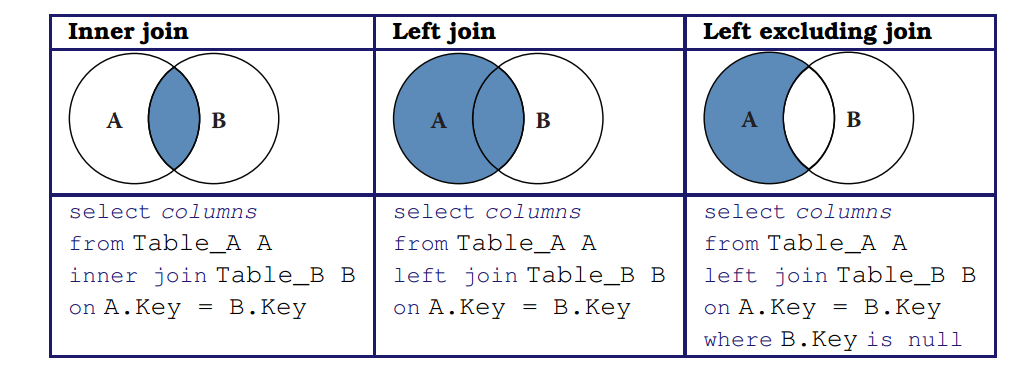
\includegraphics[width=0.7\linewidth]{ChapterDB/figures/fig-venn} 

}

\caption{Three types of *join* illustrated: the inner join, as used in Section 4.3.2, the left join, and left excluding join}\label{fig:fig-venn}
\end{figure}

\begin{center}\rule{0.5\linewidth}{\linethickness}\end{center}

\section{Which database to use?}\label{which-database-to-use}

The question of which DBMS to use for a social sciences data management
and analysis project depends on many factors. We introduced some
relevant rules in Table \ref{tab:table4-1}. We expand on those
considerations here.

\subsection{Relational DBMSs}\label{relational-dbmss-1}

If your data are structured, then a relational DBMS is almost certainly
the right technology to use. Many open source, commercial, and
cloud-hosted relational DBMSs exist. Among the open source DBMSs, MySQL
and PostgreSQL (often simply Postgres) are particularly widely used.
MySQL is the most popular. It is particularly easy to install and use,
but does not support all features of the SQL standard. PostgreSQL is
fully standard compliant and supports useful features such as full text
search and the PostGIS extensions mentioned in the previous section, but
can be more complex to work with.

Popular commercial relational DBMSs include IBM DB2, Microsoft SQL
Server, and Oracle RDMS. These systems are heavily used in commercial
settings. There are free community editions, and some large science
projects use enterprise features via licensing: for example, the Sloan
Digital Sky Survey uses Microsoft SQL Server (Szalay et al.
\protect\hyperlink{ref-szalay2002sdss}{2002}) and the CERN high-energy
physics lab uses Oracle (Girone
\protect\hyperlink{ref-girone2008cern}{2008}).

We also see increasing use being made of cloud-hosted relational DBMSs
such as Amazon Relational Database Service (RDS; this supports MySQL,
PostgreSQL, and various commercial DBMSs), Microsoft Azure, and Google
Cloud SQL. These systems obviate the need to install local software,
administer a DBMS, or acquire hardware to run and scale your database.
Particularly if your database is bigger than can fit on your
workstation, a cloud-hosted solution can be a good choice.

\subsection{NoSQL DBMSs}\label{nosql-dbmss}

Few social science problems have the scale that might motivate the use
of a NoSQL DBMS. Furthermore, while defining and enforcing a schema can
involve some effort, the benefits of so doing are considerable. Thus,
the use of a relational DBMS is usually to be recommended.

Nevertheless, as noted in Section~\protect\hyperlink{sec:db:when}{4.2},
there are occasions when a NoSQL DBMS can be a highly effective, such as
when working with large quantities of unstructured data. For example,
researchers analyzing large collections of Twitter messages frequently
store the messages in a NoSQL document-oriented database such as
MongoDB. NoSQL databases are also often used to organize large numbers
of records from many different sources, as illustrated in
Figure~\ref{fig:figdb-dbs}.

\section{Summary}\label{summary-1}

A key message of this book is that you should, whenever possible, use a
database. Database management systems are one of the great achievements
of information technology, permitting large amounts of data to be stored
and organized so as to allow rapid and reliable exploration and
analysis. They have become a central component of a great variety of
applications, from handling transactions in financial systems to serving
data published in websites. They are particularly well suited for
organizing social science data and for supporting analytics for data
exploration.

DBMSs provide an environment that greatly simplifies data management and
manipulation. They make many easy things trivial, and many hard things
easy. They automate many other error-prone, manual tasks associated with
query optimization. While they can by daunting to those unfamiliar with
their concepts and workings, they are in fact easy to use. A basic
understanding of databases and of when and how to use DBMSs is an
important element of the social data scientist's knowledge base.

\section{Resources}\label{resources-1}

The enormous popularity of DBMSs means that there are many good books to
be found. Classic textbooks such as those by Silberschatz et
al.~(Silberschatz, Korth, and Sudarshan
\protect\hyperlink{ref-silberschatz2010database}{2010}) and Ramakrishnan
and Gherke (Ramakrishnan and Gehrke
\protect\hyperlink{ref-ramakrishnan2000database}{2002}) provide a great
deal of technical detail. The DB Engines website collects information on
DBMSs (Solid IT, n.d.). There are also many also useful online
tutorials, and of course StackExchange and other online forums often
have answers to your technical questions.

Turning to specific technologies, the \emph{SQL Cookbook} (Molinaro
\protect\hyperlink{ref-SQLCookbook}{2005}) provides a wonderful
introduction to SQL. We also recommend the SQL Cheatsheet (Art Branch
Inc., n.d.) and a useful visual depiction of different SQL join
operators (Moffatt \protect\hyperlink{ref-vizjoins}{1999}). Two good
books on the PostGIS geospatial extensions to the PostgreSQL database
are the \emph{PostGIS Cookbook} (Corti et al.
\protect\hyperlink{ref-PostGISCookbook}{2014}) and \emph{PostGIS in
Action} (Obe and Hsu \protect\hyperlink{ref-PostGISInAction}{2015}). The
online documentation is also excellent (PostGIS Project Steering
Committee, n.d.). The monograph \emph{NoSQL Databases} (Strauch
\protect\hyperlink{ref-NoSQLdatabases}{2009}) provides much useful
technical detail.

We did not consider in this chapter the native extensible Markup
Language (XML) and Resource Description Framework (RDF) triple stores,
as these are not typically used for data management. However, they do
play a fundamental role in metadata and knowledge management. See, for
example, Sesame (Broekstra, Kampman, and Van Harmelen
\protect\hyperlink{ref-broekstra2002sesame}{2002}; Sesame, n.d.)

If you are interested in the state of database and data management
research, the recent Beckman Report (Abadi et al.
\protect\hyperlink{ref-abadi2014beckman}{2014}) provides a useful
perspective.

\chapter{Scaling up through Parallel and Distributed
Computing}\label{chap:parallel}

\textbf{Huy Vo and Claudio Silva}

This chapter provides an overview of techniques that facilitate the use
of large amounts of data (often using parallel computing). While the
focus is on widely used big data programming paradigm (MapReduce) and
popular implementations such as Apache Hadoop and Spark, the goal the
chapter is to provide a conceptual framework to the key challenges that
the approach is designed to address.

This chapter will describe:

\begin{itemize}
\item
  Why we need mapreduce
\item
  What is mapreduce
\item
  How to use it
\item
  Hadoop
\item
  spark
\item
  Benefits and challenges
\item
  Examples
\item
  Where the computer is
\item
  Where the data is: one disk, or distributed
\item
  Single processor
\item
  multiprocessor
\item
  distributed/parallel
\item
  laptop/Desktop
\item
  mapreduce/hadoop
\item
  Server in IT center
\item
  mapreduce/hadoop
\item
  Cloud - AWS, Azure, Google
\item
  mapreduce/hadoop
\end{itemize}

\section{Introduction}\label{introduction-1}

Why we need parallel computing for social sciences? What happens when
you use traditional programming approaches with data that's too large to
fit into memory on one computer? Or when doing analysis on one computer
will just take too long? Today, when dealing with these scenarios,
social scientists might perform sampling and analyze a subset of the
data or reduce the type and size of analysis that are done. The
techniques described in this chapter allows us to scale the analysis by
using all the data and run a larger number of \ldots{} Network analysis
Record linkage ML methods can be parallelized

\textbf{This chapter will describe:} * Why we need mapreduce * What is
mapreduce * How to use it * Hadoop * spark * Benefits and challenges *
Examples

Parallel computing to deal with large amounts of data are hardly new
ideas for dealing with computational challenges. Scientists have
routinely been working on data sets much larger than a single machine
can handle for several decades, especially at the DOE National
Laboratories (Sethian et al. \protect\hyperlink{ref-bigdata_old1}{1991};
Crossno, Cline, and Jortner
\protect\hyperlink{ref-crossno1993heterogeneous}{1993}) where
high-performance computing has been a major technology trend. This is
also demonstrated by the history of research in distributed computing
and data management going back to the 1980s (Wikipedia, n.d.).

There are many ways to do distributed and parallel computing, ranging
from completely flexible (but more complex to use) approaches such as
Message Passing Interface (MPI) (Gropp, Lusk, and Skjellum
\protect\hyperlink{ref-mpi}{2014}) to more restrictive (but much easier
to use) approaches such as MapReduce. MPI allows you to do anything with
as much efficiency as your MPI skills allow you to code while MapReduce
allows a more restrictive set of analysis to be done (possibly less
efficiently) but is much easier to learn and implement.

\section{MapReduce}\label{sec:intro}

The MapReduce framework only supports two operations: map and reduce. We
provide an overview of the MapReduce paradigm and its most popular
implementation, Apache Hadoop. MapReduce framework was proposed by
Jeffrey Dean and Sanjay Ghemawat at Google in 2004 (Dean and Ghemawat
\protect\hyperlink{ref-MapReduce}{2004}). Its origins date back to
conceptually similar approaches first described in the early 1980s.
MapReduce was indeed inspired by the \emph{map} and \emph{reduce}
functions of functional programming, though its \texttt{reduce} function
is more of a \emph{group-by-key} function, producing a list of values,
instead of the traditional reduce, which outputs only a single value.
MapReduce is a record-oriented model, where each record is treated as a
\emph{key--value} pair; thus, both and functions operate on key--value
pair data.

A typical MapReduce job is composed of three phases---map, shuffle, and
reduce---taking a list of key--value pairs
\texttt{{[}(k\$\_1\$,v\$\_2\$),\ (k\$\_2\$,v\$\_2\$),\ ...,\ (k\$\_n\$,v\$\_n\$){]}}
as input. In the map phase, each input key--value pair is run through
the \texttt{map} function, and zero or more new key--value pairs are
output. In the shuffle phase, the framework sorts the outputs of the map
phase, grouping pairs by keys before sending each of them to the
\texttt{reduce} function. In the reduce phase, each grouping of values
are processed by the \texttt{reduce} function, and the result is a list
of new values that are collected for the job output.

In brief, a MapReduce job just takes a list of key--value pairs as input
and produces a list of values as output. Users only need to implement
interfaces of the \texttt{map} and \texttt{reduce} functions (the
shuffle phase is not very customizable) and can leave it up to the
system that implements MapReduce to handle all data communications and
parallel computing. We can summarize the MapReduce logic as follows:

\textbf{map}: \((k_i, v_i)\) →
\([f(k^{'}_{i1}, v^{'}_{i1}),f(k^{'}_{i2}, v^{'}_{i2}),..]\) for a
user-defined function \(f\).

\textbf{reduce}: \((k^{''}_{i}, [v^{''}_{i1},v^{''}_{i2},..])\) →
\([v^{'''}_{1},v^{'''}_{2},..]\) where
\(\{k^{'}_{i}\} \equiv \{k^{''}_{j}\}\) and \(v^{'''} = g(v^{''})\) for
a user-defined function \(g\).

\enlargethispage{12pt}

\begin{center}\rule{0.5\linewidth}{\linethickness}\end{center}

\textbf{Example: Counting NSF awards}

To gain a better understanding of these MapReduce operators, imagine
that we have a list of NSF principal investigators, along with their
email information and award IDs as below. Our task is to count the
number of awards for each institution. For example, given the four
records below, we will discover that the Berkeley Geochronology Center
has two awards, while New York University and the University of Utah
each have one.

\begin{verbatim}
AwardId,FirstName,LastName,EmailAddress
0958723,Roland,Mundil,rmundil@bgc.org
0958915,Randall,Irmis,irmis@umnh.utah.edu
1301647,Zaher,Hani,zh8@nyu.edu
1316375,David,Shuster,dshuster@bgc.org
\end{verbatim}

We observe that institutions can be distinguished by their email address
domain name. Thus, we adopt of a strategy of first grouping all award
IDs by domain names, and then counting the number of distinct award
within each group. In order to do this, we first set the function to
scan input lines and extract institution information and award IDs.
Then, in the function, we simply count unique IDs on the data, since
everything is already grouped by institution. Python pseudo-code is
provided in Listing 5.1.

\begin{Shaded}
\begin{Highlighting}[]
\CommentTok{# Input  : a list of text lines}
\CommentTok{# Output : a list of domain name and award ids}
\NormalTok{def }\KeywordTok{MAP}\NormalTok{(lines)}\OperatorTok{:}
\StringTok{    }\ControlFlowTok{for}\NormalTok{ line }\ControlFlowTok{in}\NormalTok{ lines}\OperatorTok{:}
\StringTok{        }\NormalTok{fields     =}\StringTok{ }\KeywordTok{line.strip}\NormalTok{(}\StringTok{'}\CharTok{\textbackslash{}n}\StringTok{'}\NormalTok{)}\KeywordTok{.split}\NormalTok{(}\StringTok{','}\NormalTok{)}
\NormalTok{        awardId    =}\StringTok{ }\NormalTok{fields[}\DecValTok{0}\NormalTok{]}
\NormalTok{        domainName =}\StringTok{ }\NormalTok{fields[}\DecValTok{3}\NormalTok{]}\KeywordTok{.split}\NormalTok{(}\StringTok{'@'}\NormalTok{)[}\OperatorTok{-}\DecValTok{1}\NormalTok{]}\KeywordTok{.split}\NormalTok{(}\StringTok{'.'}\NormalTok{)[}\OperatorTok{-}\DecValTok{2}\OperatorTok{:}\NormalTok{]}
        \KeywordTok{yield}\NormalTok{ (domainName, awardId)}

\CommentTok{# Input  : a list of domain name and award ids}
\CommentTok{# Output : a list of domain name and award count}
\NormalTok{def }\KeywordTok{REDUCE}\NormalTok{(pairs)}\OperatorTok{:}
\StringTok{    }\ControlFlowTok{for}\NormalTok{ (domainName, awardIds) }\ControlFlowTok{in}\NormalTok{ pairs}\OperatorTok{:}
\StringTok{        }\NormalTok{count =}\StringTok{ }\KeywordTok{len}\NormalTok{(}\KeywordTok{set}\NormalTok{(awardIds))}
        \KeywordTok{yield}\NormalTok{ (domainName, count)}
\end{Highlighting}
\end{Shaded}

Listing 5.1. Python pseudo-code for the \texttt{map} and \texttt{reduce}
functions to count the number of awards per institution

In the map phase, the input will be transformed into tuples of
institutions and award ids:

\texttt{"0958723,Roland,Mundil,rmundil@bgc.org"} →
\texttt{("bgc.org",\ 0958723)}
\texttt{"0958915,Randall,Irmis,irmis@umnh.utah.edu"} →
\texttt{("utah.edu",\ 0958915)}
\texttt{"1301647,Zaher,Hani,zh8@nyu.edu"} →
\texttt{("nyu.edu",\ 1301647)}
\texttt{"1316375,David,Shuster,dshuster@bgc.org"} →
\texttt{("bgc.org",\ 1316375)}

Then the tuples will be grouped by institutions and be counted by the
function.

\texttt{("bgc.org",\ {[}0958723,1316375{]})} → \texttt{("bgc.org",\ 2)}
\texttt{("utah.edu",\ \textbackslash{}{[}0958915\textbackslash{}{]})} →
\texttt{("utah.edu",\ 1)}
\texttt{("nyu.edu",\ \textbackslash{}{[}1301647\textbackslash{}{]})} →
\texttt{("nyu.edu",\ 1)}

\pagebreak
As we have seen so far, the MapReduce programming model is quite simple
and straightforward, yet it supports a simple parallelization model. In
fact, it has been said to be \emph{too} simple and criticized as ``a
major step backwards'' (DeWitt and Stonebraker
\protect\hyperlink{ref-MapReduceBad}{2008}) for large-scale,
data-intensive applications. It is hard to argue that MapReduce is
offering something truly innovative when MPI has been offering similar
scatter and reduce operations since 1995, and Python has had high-order
functions (\texttt{map}, \texttt{reduce}, \texttt{filter}, and
\texttt{lambda}) since its 2.2 release in 1994. However, the biggest
strength of MapReduce is its simplicity. Its simple programming model
has brought many non-expert users to big data analysis. Its simple
architecture has also inspired many developers to develop advanced
capabilities, such as support for distributed computing, data
partitioning, and streaming processing. (A downside of this diversity of
interest is that available features and capabilities can vary
considerably, depending on the specific implementation of MapReduce that
is being used.)

As mentioned above, MapReduce is a programming model. In order to
implement an analysis in MapReduce, we need to select an implementation
of MapReduce. Two most commonly used n implementations of the MapReduce
model are Hadoop and Spark, that we describe in more detail below.

\section{Apache Hadoop MapReduce}\label{apache-hadoop-mapreduce}

Apache Hadoop (or Hadoop)\footnote{The term \emph{Hadoop} refers to the
  creator's son's toy elephant.} was originally designed to run in
environments with thousands of machines. Supporting such a large
computing environment puts several constraints on the system; for
instance, with so many machines, the system had to assume computing
nodes would fail. Hadoop is an enhanced MapReduce implementation with
the support for fault tolerance, distributed storage, and data
parallelism through two added key design features: (1) a distributed
file system called the Hadoop Distributed File System (HDFS); and (2) a
data distribution strategy that allows computation to be moved to the
data during execution.

\subsection{The Hadoop Distributed File
System}\label{the-hadoop-distributed-file-system}

The Hadoop Distributed File System ({\textbf{???}})(Apache Hadoop, n.d.)
is a distributed file system that stores data across all the nodes
(machines) of a Hadoop cluster. HDFS splits large data files into
smaller blocks (chunks of data) which are managed by different nodes in
a cluster. Each block is also replicated across several nodes as an
attempt to ensure that a full copy of the data is still available even
in the case of computing node failures. The block size as well as the
number of replications per block are fully customized by users when they
create files on HDFS. By default, the block size is set to 64 MB with a
replication factor of 3, meaning that the system may encounter at least
two concurrent node failures without losing any data. HDFS also actively
monitors failures and re-replicates blocks on failed nodes to make sure
that the number of replications for each block always stays at the
user-defined settings. Thus, if a node fails, and only two copies of
some data exist, the system will quickly copy those data to a working
node, thus raising the number of copies to three again. This dynamic
replication the primary mechanism for fault tolerance in Hadoop.

Note that data blocks are replicated and distributed across several
machines. This could create a problem for users, because if they had to
manage the data manually, they might, for example, have to access more
than one machine to fetch a large data file. Fortunately, Hadoop
provides infrastructure for managing this complexity seamlessly,
including command line programs as well as an API that users can employ
to interact with HDFS as if it were a local file system. For example,
one can run simple linux commands such as ls and mkdir to list and
create a directory on HDFS, or even use to inspect file contents the
same way as one would do in a Linux file system. The following code
shows some examples of interacting with HDFS.

\hypertarget{lst:hdfs}{\label{lst:hdfs}}
\begin{verbatim}
# Creating a folder
hadoop dfs -mkdir /hadoopiseasy

# Upload a CSV file from our local machine to HDFS
hadoop dfs -put importantdata.csv /hadoopiseasy

# Listing all files under hadoopiseasy folder
hadoop dfs -ls /hadoopiseasy

# Download a file to our local machine
hadoop dfs -get /hadoopiseasy/importantdata.csv
\end{verbatim}

\subsection{Hadoop Setup: Bringing compute to the
data}\label{hadoop-setup-bringing-compute-to-the-data}

There are two parts of the computing environment when using Hadoop: a
\emph{compute cluster} with substantial computing power (e.g., thousands
of computing cores) 2. a \emph{storage cluster} with lots of disk space,
capable of storing and serving data quickly to the compute cluster.

These two clusters have quite different hardware specifications: the
first is optimized for CPU performance and the second for storage. The
two systems are typically configured as separate physical hardware.

\begin{center}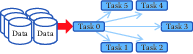
\includegraphics[width=0.7\linewidth]{ChapterParallel/figures/data2compute} \end{center}\begin{figure}

{\centering 
\includegraphics[width=0.7\linewidth]{ChapterParallel/figures/compute2data} 

}

\caption{Top: The traditional parallel computing model where data are brought to the computing nodes. Bottom: Hadoop’s parallel computing model: bringing compute to the data [@HadoopParallelModel]}\label{fig:fig5-1a}
\end{figure}

Running compute jobs on such hardware often goes like this. When a user
requests to run an intensive task on a particular data set, the system
will first reserve a set of computing nodes. Then the data are
partitioned and copied from the storage server into these computing
nodes before the task is executed. This process is illustrated in Figure
\ref{fig:fig5-1a} (top). This computing model will be referred to as
\emph{bringing data to computation}. In this model, if a data set is
being analyzed in multiple iterations, it is very likely that the data
will be copied multiple times from the storage cluster to the compute
nodes without reusability. This is because the compute node scheduler
normally does not have or keep knowledge of where data have previously
been held. The need to copy data multiple times tends to make such a
computation model inefficient, and I/O becomes the bottleneck when all
tasks constantly pull data from the storage cluster (the green arrow).
This in turn leads to poor scalability; adding more nodes to the
computing cluster would not increase its performance.

To solve this problem, Hadoop implements a \emph{bring compute to the
data} strategy that combines both computing and storage at each node of
the cluster. In this setup, each node offers both computing power and
storage capacity. As shown in Figure \ref{fig:fig5-1a} (bottom), when
users submit a task to be run on a data set, the scheduler will first
look for nodes that contain the data, and if the nodes are available, it
will schedule the task to run directly on those nodes. If a node is busy
with another task, data will still be copied to available nodes, but the
scheduler will maintain records of the copy for subsequent use of the
data. In addition, data copying can be minimized by increasing the data
duplication in the cluster, which also increases the potential for
parallelism, since the scheduler has more choices to allocate computing
without copying. Since both the compute and data storage are closely
coupled for this model, it is best suited for data-intensive
applications.

Given that Hadoop was designed for batch data processing at scale, this
model fits the system nicely, especially with the support of HDFS.
However, in an environment where tasks are more compute intensive, a
traditional high-performance computing environment is probably best
since it tends to spend more resources on CPU cores. It should be clear
now that the Hadoop model has hardware implications, and computer
architects have optimized systems for data-intensive computing.

\subsection{Hardware provisioning}\label{hardware-provisioning}

Hadoop requires a distributed cluster of machines to operate
efficiently. (It can be set up to run entirely on a single computer, but
this should only be done for technology demonstration purposes.) This is
mostly because the MapReduce performance heavily depends on the total
I/O throughput (i.e., disk read and write) of the entire system. Having
a distributed cluster, where each machine has its own set of hard
drives, is one of the most efficient ways to maximize this throughput.

A typical Hadoop cluster consists of two types of machine: masters and
workers. Master machines are those exclusively reserved for running
services that are critical to the framework operations. Some examples
are the NameNode and the JobTracker services, which are tasked to manage
how data and tasks are distributed among the machines, respectively. The
worker machines are reserved for data storage and for running actual
computation tasks (i.e., map and reduce). It is normal to have worker
machines that can be included or removed from an operational cluster on
demand. This ability to vary the number of worker nodes makes the
overall system more tolerant of failure. However, master machines are
usually required to be running uninterrupted.

Provisioning and configuring the hardware for Hadoop, like any other
parallel computing, are some of the most important and complex tasks in
setting up a cluster, and they often require a lot of experience and
careful consideration. Major big data vendors provide guidelines and
tools to facilitate the process (Apache Software Foundation, n.d.;
Cloudera, n.d.; Baldeschwieler
\protect\hyperlink{ref-Provisioning}{2011}). most decisions will be
based on the types of analysis to be run on the cluster, for which only
you, as the user, can provide the best input.

\subsection{Programming in Hadoop}\label{programming-in-hadoop}

Now that we are equipped with the knowledge that Hadoop is a MapReduce
implementation that runs on HDFS and a bring-compute-to-the-data model,
we can go over the design of a Hadoop MapReduce job. A MapReduce job is
still composed of three phases: map, shuffle, and reduce. However,
Hadoop divides the map and reduce phases into smaller tasks.

Each map phase in Hadoop is divided into five tasks: \textbf{input
format}, \textbf{record reader}, \textbf{mapper}, \textbf{combiner}, and
\textbf{partitioner}. An {input format} task is in charge of talking to
the input data presumably sitting on HDFS, and splitting it into
partitions (e.g., by breaking lines at line breaks). Then a {record
reader} task is responsible for translating the split data into the
key--value pair records so that they can be processed by the mapper. By
default, Hadoop parses files into key--value pairs of line numbers and
line contents. However, both input formats and record readers are fully
customizable and can be programmed to read custom data including binary
files. It is important to note that input formats and record readers
only provide data partitioning; they do not move data around computing
nodes.

After the records are generated, mappers are spawned---typically on
nodes containing the blocks---to run through these records and output
zero or more new key--value pairs. A mapper in Hadoop is equivalent to
the \texttt{map} function of the MapReduce model that we discussed
earlier. The selection of the key to be output from the mapper will
heavily depend on the data processing pipeline and could greatly affect
the performance of the framework. Mappers are executed concurrently in
Hadoop as long as resources permit.

A combiner task in Hadoop is similar to a function in the MapReduce
framework, but it only works locally at each node: it takes output from
mappers executed on the same node and produces aggregated values.
Combiners are optional but can be used to greatly reduce the amount of
data exchange in the shuffle phase; thus, users are encouraged to
implement this whenever possible. A common practice is when a
\texttt{reduce} function is both commutative and associative, and has
the same input and output format, one can just use the \texttt{reduce}
function as the combiner. Nevertheless, combiners are not guaranteed to
be executed by Hadoop, so this should only be treated as a hint. Its
execution must not affect the correctness of the program.

A partitioner task is the last process taking place in the map phase on
each mapper node, where it hashes the key of each key--value pair output
from the mappers or the combiners into bins. By default, the partitioner
uses object hash codes and modulus operations to direct a designated
reducer to pull data from a map node. Though it is possible to customize
the partitioner, it is only advisable to do so when one fully
understands the intermediate data distribution as well as the
specifications of the cluster. In general, it is better to leave this
job to Hadoop.

Each reduce phase in Hadoop is divided into three tasks:
\textbf{reducer}, \textbf{output format}, and \textbf{record writer}.
The \texttt{reducer} task is equivalent to the \texttt{reduce} function
of the MapReduce model. It basically groups the data produced by the
mappers by keys and runs a \texttt{reduce} function on each list of
grouping values. It outputs zero or more key--value pairs for the output
format task, which then translates them into a writable format for the
record writer task to serialize on HDFS. By default, Hadoop will
separate the key and value with a tab and write separate records on
separate lines. However, this behavior is fully customizable. Similarly,
the map phase reducers are also executed concurrently in Hadoop.

\begin{figure}

{\centering 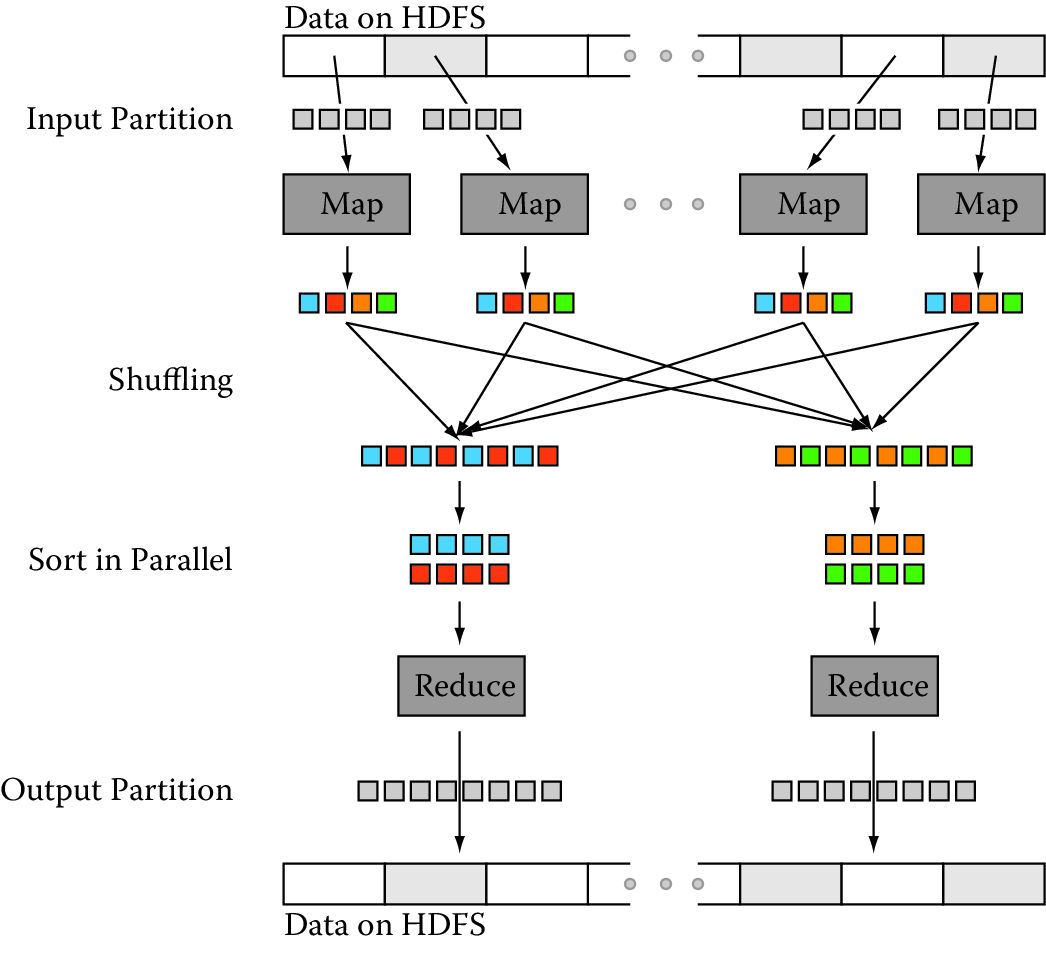
\includegraphics[width=0.7\linewidth]{ChapterParallel/figures/hadoop} 

}

\caption{Data transfer and communication of a MapReduce job in Hadoop. Data blocks are assigned to several maps, which emit key--value pairs that are shuffled and sorted in parallel. The reduce step emits one or more pairs, with results stored on the HDFS}\label{fig:hadoop}
\end{figure}

\subsection{Programming language
support}\label{programming-language-support}

\enlargethispage{6pt} Hadoop is written entirely in Java, thus it is
best supporting applications written in Java. However, Hadoop also
provides a \emph{streaming API} that allows arbitrary code to be run
inside the Hadoop MapReduce framework through the use of UNIX pipes.
This means that we can supply a mapper program written in Python or C++
to Hadoop as long as that program reads from the standard input and
writes to the standard output. The same mechanism also applies for the
combiner and reducer. For example, we can develop from the Python
pseudo-code in Listing 5.1 to a complete Hadoop streaming mapper
(Listing 5.2) and reducer (Listing 5.3).

\hypertarget{lst:mapper}{\label{lst:mapper}}
\begin{verbatim}
#!/usr/bin/env python
import sys

def parseInput():
    for line in sys.stdin:
        yield line

if __name__=='__main__':
    for line in parseInput():
        fields     = line.strip('\n').split(',')
        awardId    = fields[0]
        domainName = fields[3].split('@')[-1].split('.')[-2:]
        print('%s\t%s' % (domainName,awardId))
\end{verbatim}

Listing 5.2. A Hadoop streaming mapper in Python

\hypertarget{lst:reducer}{\label{lst:reducer}}
\begin{verbatim}
#!/usr/bin/env python
import sys

def parseInput():
    for line in sys.stdin:
        yield line

if __name__=='__main__':
    for line in parseInput():
        (domainName, awardIds) = line.split('\t')
        count = len(set(awardIds))
        print('%s\t%s' % (domainName, count))
\end{verbatim}

Listing 5.3. A Hadoop streaming reducer in Python

It should be noted that in Hadoop streaming, intermediate key--value
pairs (the data flowing between mappers and reducers) must be in
tab-delimited format, thus we replace the original \texttt{yield}
command with a \texttt{print} formatted with tabs. Though the input
format and record reader are still customizable in Hadoop streaming,
they must be supplied as Java classes. This is one of the biggest
limitations of Hadoop for Python developers. They not only have to split
their code into separate mapper and reducer programs, but also need to
learn Java if they want to work with nontextual data.

\subsection{Benefits and Limitations of
Hadoop}\label{benefits-and-limitations-of-hadoop}

\begin{itemize}
\item
  \textbf{Fault Tolerance}: By default, HDFS uses checksums to enforce
  data integrity on its file system use data replication for recovery of
  potential data losses. Taking advantage of this, Hadoop also maintains
  fault tolerance of MapReduce jobs by storing data at every step of a
  MapReduce job to HDFS, including intermediate data from the combiner.
  Then the system checks whether a task fails by either looking at its
  heartbeats (data activities) or whether it has been taking too long.
  If a task is deemed to have failed, Hadoop will kill it and run it
  again on a different node. The time limit for the heartbeats and task
  running duration may also be customized for each job. Though the
  mechanism is simple, it works well on thousands of machines. It is
  indeed highly robust because of the simplicity of the model.
\item
  \textbf{Performance}: Hadoop has proven to be a scalable
  implementation that can run on thousands of cores. However, it is also
  known for having a relatively high job setup overheads and suboptimal
  running time. An empty task in Hadoop (i.e., with no mapper or
  reducer) can take roughly 30 seconds to complete even on a modern
  cluster. This overhead makes it unsuitable for real-time data or
  interactive jobs. The problem comes mostly from the fact that Hadoop
  monitoring processes only lives within a job, thus it needs to start
  and stop these processes each time a job is submitted, which in turns
  results in this major overhead. Moreover, the brute force approach of
  maintaining fault tolerance by storing everything on HDFS is
  expensive, especially when for large data sets.
\item
  \textbf{Hadoop streaming support for non-Java applications}: As
  mentioned previously, non-Java applications may only be integrated
  with Hadoop through the Hadoop streaming API. However, this API is far
  from optimal. First, input formats and record readers can only be
  written in Java, making it impossible to write advanced MapReduce jobs
  entirely in a different language. Second, Hadoop streaming only
  communicates with Hadoop through Unix pipes, and there is no support
  for data passing within the application using native data structure
  (e.g., it is necessary to convert Python tuples into strings in the
  mappers and convert them back into tuples again in reducers).
\item
  \textbf{Real-time applications}: With the current setup, Hadoop only
  supports batch data processing jobs. This is by design, so it is not
  exactly a limitation of Hadoop. However, given that more and more
  applications are dealing with real-time massive data sets, the
  community using MapReduce for real-time processing is constantly
  growing. Not having support for streaming or real-time data is clearly
  a disadvantage of Hadoop over other implementations.
\item
  \textbf{Limited data transformation operations}: This is more of a
  limitation of MapReduce than Hadoop per se. MapReduce only supports
  two operations, map and reduce, and while these operations are
  sufficient to describe a variety of data processing pipelines, there
  are classes of applications that MapReduce is not suitable for. Beyond
  that, developers often find themselves rewriting simple data
  operations such as data set joins, finding a min or max, and so on.
  Sometime, these tasks require more than one map-and-reduce operation,
  resulting in multiple MapReduce jobs. This is both cumbersome and
  inefficient. There are tools to automate this process for Hadoop;
  however, they are only a layer above, and it is not easy to integrate
  with existing customized Hadoop applications.
\end{itemize}

\section{Other MapReduce
Implementations}\label{other-mapreduce-implementations}

In addition to Apache Hadoop, other notable MapReduce implementations
include MongoDB, GreenplumDB, Disco, Riak, and Spark. MongoDB, Riak, and
Greenplum DB are all database systems\footnote{See Chapter 4.} and thus
their MapReduce implementations focus more on the interoperability of
MapReduce and the core components such as MongoDB's aggregation
framework, and leave it up to users to customize the MapReduce
functionalities for broader tasks. Some of these systems, such as Riak,
only parallelize the map phase, and run the reduce phase on the local
machine that request the tasks. The main advantage of the three
implementations is the ease with which they connect to specific data
stores. However, their support for general data processing pipelines is
not as extensive as that of Hadoop.

Disco, similar to Hadoop, is designed to support MapReduce in a
distributed computing environment, but it written in Erlang with a
Python interface. Thus, for Python developers, Disco might be a better
fit. However, it has significantly fewer supporting applications, such
as access control and workflow integration, as well as a smaller
developing community. This is why the top three big data platforms,
Cloudera, Hortonworks, and MapR, still build primarily on Hadoop.

\section{Apache Spark}\label{apache-spark}

Apache Spark is another implementation that aims to support beyond
MapReduce. The framework is centered around the concept of resilient
distributed data sets and data transformations that can operate on these
objects. An innovation in Spark is that the fault tolerance of resilient
distributed data sets can be maintained without flushing data onto
disks, thus significantly improving the system performance (with a claim
of being 100 times faster than Hadoop). Instead, the fault-recovery
process is done by replaying a log of data transformations on
check-point data. Though this process could take longer than reading
data straight from HDFS, it does not occur often and is a fair tradeoff
between processing performance and recovery performance.

Beyond map and reduce, Spark also supports various other transformations
(Hadoop, n.d.), including filter, data join, and aggregation. Streaming
computation can also be done in Spark by asking Spark to reserve
resources on a cluster to constantly stream data to/from the cluster.
However, this streaming method might be resource intensive (still
consuming resources when there is no data coming). Additionally, Spark
plays well with the Hadoop ecosystem, particularly with the distributed
file system (HDFS) and resource manager (YARN), making it possible to be
built on top of current Hadoop applications.

Another advantage of Spark is that it supports Python natively; thus,
developers can run Spark in a fraction of the time required for Hadoop.
Listing 5.4 provides the full code for the previous example written
entirely in Spark. It should be noted that Spark's concept of the
\texttt{reduceByKey} operator is not the same as Hadoop's, as it is
designed to aggregate all elements of a data set into a single element.
The closest simulation of Hadoop's MapReduce pattern is a combination of
\texttt{mapPartitions}, \texttt{groupByKey} and \texttt{mapPartitions},
as shown in the next example.

\hypertarget{lst:spark}{\label{lst:spark}}
\begin{verbatim}
import sys
from pyspark import SparkContext
def mapper(lines):
    for line in lines:
        fields     = line.strip('\n').split(',')
        awardId    = fields[0]
        domainName = fields[3].split('@')[-1].split('.')[-2:]
        yield (domainName, awardId)

def reducer(pairs):
    for (domainName, awardIds) in pairs:
        count = len(set(awardIds))
        yield (domainName, count)

if __name__=='__main__':
    hdfsInputPath  = sys.argv[1]
    hdfsOutputFile =  sys.argv[2]
    sc = SparkContext(appName="Counting Awards")
    output = sc.textFile(hdfsInputPath) \
        .mapPartitions(mapper) \
        .groupByKey() \
        .mapPartitions(reducer)

    output.saveAsTextFile(hdfsInputPath)
\end{verbatim}

Listing 5.4. Python code for a Spark program that counts the number of
awards per institution using MapReduce

\begin{center}\rule{0.5\linewidth}{\linethickness}\end{center}

\textbf{Example: Analyzing home mortgage disclosure application data}

We use a financial services analysis problem to illustrate the use of
Apache Spark.

Mortgage origination data provided by the Consumer Protection Financial
Bureau provide insightful details of the financial health of the real
estate market. The data (Consumer Financial Protection Bureau, n.d.),
which are a product of the Home Mortgage Disclosure Act (HMDA),
highlight key attributes that function as strong indicators of health
and lending patterns.

Lending institutions, as defined by section 1813 in Title 12 of the
HMDA, decide on whether to originate or deny mortgage applications based
on credit risk. In order to determine this credit risk, lenders must
evaluate certain features relative to the applicant, the underlying
property, and the location. We want to determine whether census tract
clusters could be created based on mortgage application data and whether
lending institutions' perception of risk is held constant across the
entire USA.

For the first step of this process, we study the debt--income ratio for
loans originating in different census tracts. This could be achieved
simply by computing the debt--income ratio for each loan application and
aggregating them for each year by census tract number. A challenge,
however, is that the data set provided by HMDA is quite extensive. In
total, HMDA data contain approximately 130 million loan applications
between 2007 and 2013. As each record contains 47 attributes, varying in
types from continuous variables such as loan amounts and applicant
income to categorical variables such as applicant gender, race, loan
type, and owner occupancy, the entire data set results in about 86 GB of
information. Parsing the data alone could take up to hours on a single
machine if using a naïve approach that scans through the data
sequentially. Tables \ref{tab:table5-1} and \ref{tab:table5-2} highlight
the breakdown in size per year and data fields of interest.

\begin{longtable}[]{@{}ccc@{}}
\caption{\label{tab:table5-1} Home Mortgage Disclosure Act data
size}\tabularnewline
\toprule
\textbf{Year} & \textbf{Records} & \textbf{File Size
(Gigabytes)}\tabularnewline
\midrule
\endfirsthead
\toprule
\textbf{Year} & \textbf{Records} & \textbf{File Size
(Gigabytes)}\tabularnewline
\midrule
\endhead
2007 & 26,605,696 & 18\tabularnewline
2008 & 17,391,571 & 12\tabularnewline
2009 & 19,493,492 & 13\tabularnewline
2010 & 16,348,558 & 11\tabularnewline
2011 & 14,873,416 & 9.4\tabularnewline
2012 & 18,691,552 & 12\tabularnewline
2013 & 17,016,160 & 11\tabularnewline
\textbf{Total} & \textbf{130,420,445} & \textbf{86.4}\tabularnewline
\bottomrule
\end{longtable}

\begin{longtable}[]{@{}llc@{}}
\caption{\label{tab:table5-2} Home Mortgage Disclosure Act data
size}\tabularnewline
\toprule
\textbf{Index} & \textbf{Attribute} & \textbf{Type}\tabularnewline
\midrule
\endfirsthead
\toprule
\textbf{Index} & \textbf{Attribute} & \textbf{Type}\tabularnewline
\midrule
\endhead
0 & Year & Integer\tabularnewline
1 & State & String\tabularnewline
2 & County & String\tabularnewline
3 & Census Tract & String\tabularnewline
4 & Loan Amount & Float\tabularnewline
5 & Applicant Income & Float\tabularnewline
6 & Loan Originated & Boolean\tabularnewline
\ldots{} & \ldots{} & \ldots{}\tabularnewline
\bottomrule
\end{longtable}

Observing the transactional nature of the data, where the aggregation
process could be distributed and merged across multiple partitions of
the data, we could complete this task in much less time by using Spark.
Using a cluster consisting of 1,200 cores, the Spark program in Listing
5.5 took under a minute to complete. The substantial performance gain
comes not so much from the large number of processors available, but
mostly from the large I/O bandwidth available on the cluster thanks to
the 200 distributed hard disks and fast network interconnects.

\hypertarget{lst:hdma}{\label{lst:hdma}}
\begin{verbatim}
import ast
import sys
from pyspark import SparkContext

def mapper(lines):
    for line in lines:
        fields = ast.literal_eval('(%s)' % line)
        (year, state, county, tract) = fields[:4]
        (amount, income, originated) = fields[4:]

        key = (year, state, county, tract)
        value = (amount, income)

        # Only count originated loans
        if originated:
            yeild (key, value)

def sumDebtIncome(debtIncome1, debtIncome2):
    return (debtIncome1[0] + debtIncome2[0], debtIncome1[1] + debtIncome2[1])

if __name__=='__main__':
    hdfsInputPath  = sys.argv[1]
    hdfsOutputFile =  sys.argv[2]
    sc = SparkContext(appName="Counting Awards")
    sumValues = sc.textFile(hdfsInputPath) \
        .mapPartitions(mapper) \
        .reduceByKey(sumDebtIncome)

    # Actually compute the aggregated debt income
    output = sumValues.mapValues(lambda debtIncome: debtIncome[0]/debtIncome[1])

    output.saveAsTextFile(hdfsInputPath)
\end{verbatim}

Listing 5.5. Python code for a Spark program to aggregate the
debt--income ratio for loans originated in different census tracts

\begin{center}\rule{0.5\linewidth}{\linethickness}\end{center}

\section{Summary}\label{summary-2}

Analyzing large amounts of data means that it is necessary to both store
very large collections of data and perform aggregate computations on
those data. This chapter Describes an important data storage approach
(the Hadoop Distributed File System) and a way of processing large-scale
data sets (the MapReduce model, as implemented in both Hadoop and
Spark). This model enables not only large-scale data analysis but also
provides easy to use implementations for more flexibility for social
scientists to work with large amounts of data. This increases the
analytic throughput as well as the time to insight, speeding up the
decision-making process and thus increasing impact.

\section{Resources}\label{resources-2}

There are a wealth of online resources describing both Hadoop and Spark.
See, for example, the tutorials on the Apache Hadoop (Apache Software
Foundation, n.d.) and Spark (Apache Software Foundation, n.d.) websites.
Albanese describes how to use Hadoop for social science (Albanese,
n.d.), and Lin and Dyer discuss the use of MapReduce for text analysis
(Lin and Dyer \protect\hyperlink{ref-lin2010data}{2010}).

\hypertarget{chap:ml}{\chapter{Machine Learning}\label{chap:ml}}

\textbf{Rayid Ghani and Malte Schierholz}

This chapter introduces you to the value of machine learning in the
social sciences, particularly focusing on the overall machine learning
process as well as clustering and classification methods. You will get
an overview of the machine learning pipeline and methods and how those
methods are applied to solve social science problems. The goal is to
give an intuitive explanation for the methods and to provide practical
tips on how to use them in practice.

\section{Introduction}\label{introduction-2}

You have probably heard of ``machine learning'' but are not sure exactly
what it is, how it differs from traditional statistics, and what you can
do with it. In this chapter, we will demystify machine learning, draw
connections to what you already know from statistics and data analysis,
and go deeper into some of the unique concepts and methods that have
been developed in this field. Although the field originates from
computer science (specifically, artificial intelligence), it has been
influenced quite heavily by statistics in the past 15 years. As you will
see, many of the concepts you will learn are not entirely new, but are
simply called something else. For example, you already are familiar with
logistic regression (a classification method that falls under the
supervised learning framework in machine learning) and cluster analysis
(a form of unsupervised learning). You will also learn about new methods
that are more exclusively used in machine learning, such as random
forests and support vector machines. We will keep formalisms to a
minimum and focus on getting the intuition across, as well as providing
practical tips. Our hope is this chapter will make you comfortable and
familiar with machine learning vocabulary, concepts, and processes, and
allow you to further explore and use these methods and tools in your own
research and practice.

\section{What is machine learning?}\label{what-is-machine-learning}

When humans improve their skills with experience, they are said to
learn. Is it also possible to program computers to do the same? Arthur
Samuel, who coined the term \emph{machine learning} in 1959 (Samuel
\protect\hyperlink{ref-samuel1959some}{1959}), was a pioneer in this
area, programming a computer to play checkers. The computer played
against itself and human opponents, improving its performance with every
game. Eventually, after sufficient \emph{training} (and experience), the
computer became a better player than the human programmer. Today,
machine learning has grown significantly beyond learning to play
checkers. Machine learning systems have learned to drive (and park)
autonomous cars, are embedded inside robots, can recommend books,
products, and movies we are (sometimes) interested in, identify drugs,
proteins, and genes that should be investigated further to cure
diseases, detect cancer and other diseases in medical imaging, help us
understand how the human brain learns language, help identify which
voters are persuadable in elections, detect which students are likely to
need extra support to graduate high school on time, and help solve many
more problems. Over the past 20 years, machine learning has become an
interdisciplinary field spanning computer science, artificial
intelligence, databases, and statistics. At its core, machine learning
seeks to design computer systems that improve over time with more
experience. In one of the earlier books on machine learning, Tom
Mitchell gives a more operational definition, stating that: ``A computer
program is said to learn from experience \(E\) with respect to some
class of tasks \(T\) and performance measure \(P\), if its performance
at tasks in \(T\), as measured by \(P\), improves with experience
\(E\)'' (Mitchell \protect\hyperlink{ref-mitchell1997machine}{1997}).

\enlargethispage{6pt}

\begin{F00}
\textbf{Box 6.1: Commercial machine learning examples}

\begin{itemize}
\item
  \textbf{Speech recognition}: Speech recognition software uses machine
  learning algorithms that are built on large amounts of initial
  training data. Machine learning allows these systems to be tuned and
  adapt to individual variations in speaking as well as across different
  domains.
\item
  \textbf{Autonomous cars}: The ongoing development of self-driving cars
  applies techniques from machine learning. An onboard computer
  continuously analyzes the incoming video and sensor streams in order
  to monitor the surroundings. Incoming data are matched with annotated
  images to recognize objects like pedestrians, traffic lights, and
  potholes. In order to assess the different objects, huge training data
  sets are required where similar objects already have been identified.
  This allows the autonomous car to decide on which actions to take
  next.
\item
  \textbf{Fraud detection}: Many public and private organizations face
  the problem of fraud and abuse. Machine learning systems are widely
  used to take historical cases of fraud and flag fraudulent
  transactions as they take place. These systems have the benefit of
  being adaptive, and improving with more data over time.
\item
  \textbf{Personalized ads}: Many online stores have personalized
  recommendations promoting possible products of interest. Based on
  individual shopping history and what other similar users bought in the
  past, the website predicts products a user may like and tailors
  recommendations. Netflix and Amazon are two examples of companies
  whose recommendation software predicts how a customer would rate a
  certain movie or product and then suggests items with the highest
  predicted ratings. Of course there are some caveats here, since they
  then adjust the recommendations to maximize profits.
\item
  \textbf{Face recognition}: Surveillance systems, social networking
  platforms, and imaging software all use face detection and face
  recognition to first detect faces in images (or video) and then tag
  them with individuals for various tasks. These systems are trained by
  giving examples of faces to a machine learning system which then
  learns to detect new faces, and tag known individuals.
\end{itemize}
\end{F00}

Machine learning grew from the need to build systems that were adaptive,
scalable, and cost-effective to build and maintain. A lot of tasks now
being done using machine learning used to be done by rule-based systems,
where experts would spend considerable time and effort developing and
maintaining the rules. The problem with those systems was that they were
rigid, not adaptive, hard to scale, and expensive to maintain. Machine
learning systems started becoming popular because they could improve the
system along all of these dimensions\footnote{See Chapter 3.}. Box 6.1
mentions several examples where machine learning is being used in
commercial applications today. Social scientists are uniquely placed
today to take advantage of the same advances in machine learning by
having better methods to solve several key problems they are tackling.
We will give concrete examples later in this chapter.

This chapter is not an exhaustive introduction to machine learning.
There are many books that have done an excellent job of that (Flach
\protect\hyperlink{ref-Flach}{2012}; Hastie, Tibshirani, and Friedman
\protect\hyperlink{ref-HastieTibshirani}{2001}; Mitchell
\protect\hyperlink{ref-mitchell1997machine}{1997}). Instead, we present
a short and understandable introduction to machine learning for social
scientists, give an overview of the overall machine learning process,
provide an intuitive introduction to machine learning methods, give some
practical tips that will be helpful in using these methods, and leave a
lot of the statistical theory to machine learning textbooks. As you read
more about machine learning in the research literature or the media, you
will encounter names of other fields that are related (and practically
the same for most social science audiences), such as statistical
learning, data mining, and pattern recognition.

\section{The machine learning
process}\label{the-machine-learning-process}

When solving problems using machine learning methods, it is important to
think of the larger data-driven problem-solving process of which these
methods are a small part\footnote{See Chapter 3.}. A typical machine
learning problem requires researchers and practitioners to take the
following steps:

\begin{enumerate}
\def\labelenumi{\arabic{enumi}.}
\item
  \textbf{Understand the problem and goal}: This sounds obvious but is
  often nontrivial. Problems typically start as vague descriptions of a
  goal---improving health outcomes, increasing graduation rates,
  understanding the effect of a variable \(X\) on an outcome \(Y\), etc.
  It is really important to work with people who understand the domain
  being studied to dig deeper and define the problem more concretely.
  What is the analytical formulation of the metric that you are trying
  to optimize?
\item
  \textbf{Formulate it as a machine learning problem}: Is it a
  classification problem or a regression problem? Is the goal to build a
  model that generates a ranked list prioritized by risk, or is it to
  detect anomalies as new data come in? Knowing what kinds of tasks
  machine learning can solve will allow you to map the problem you are
  working on to one or more machine learning settings and give you
  access to a suite of methods.
\item
  \textbf{Data exploration and preparation}: Next, you need to carefully
  explore the data you have. What additional data do you need or have
  access to? What variable will you use to match records for integrating
  different data sources? What variables exist in the data set? Are they
  continuous or categorical? What about missing values? Can you use the
  variables in their original form or do you need to alter them in some
  way?
\item
  \textbf{Feature engineering}: In machine learning language, what you
  might know as independent variables or predictors or factors or
  covariates are called ``features.'' Creating good features is probably
  the most important step in the machine learning process. This involves
  doing transformations, creating interaction terms, or aggregating over
  data points or over time and space.
\item
  \textbf{Method selection}: Having formulated the problem and created
  your features, you now have a suite of methods to choose from. It
  would be great if there were a single method that always worked best
  for a specific type of problem, but that would make things too easy.
  Typically, in machine learning, you take a collection of methods and
  try them out to empirically validate which one works the best for your
  problem. We will give an overview of leading methods that are being
  used today in this chapter.
\item
  \textbf{Evaluation}: As you build a large number of possible models,
  you need a way to select the model that is the best. This part of the
  chapter will cover the validation methodology to first validate the
  models on historical data as well as discuss a variety of evaluation
  metrics. The next step is to validate using a field trial or
  experiment.
\item
  \textbf{Deployment}: Once you have selected the best model and
  validated it using historical data as well as a field trial, you are
  ready to put the model into practice. You still have to keep in mind
  that new data will be coming in, and the model might change over time.
  We will not cover too much of those aspects in this chapter, but they
  are important to keep in mind.
\end{enumerate}

\section{Problem formulation: Mapping a problem to machine learning
methods}\label{problem-formulation-mapping-a-problem-to-machine-learning-methods}

When working on a new problem, one of the first things we need to do is
to map it to a class of machine learning methods. In general, the
problems we will tackle, including the examples above, can be grouped
into two major categories:

\begin{enumerate}
\def\labelenumi{\arabic{enumi}.}
\item
  \textbf{Supervised learning}: These are problems where there exists a
  target variable (continuous or discrete) that we want to predict or
  classify data into. Classification, prediction, and regression all
  fall into this category. More formally, supervised learning methods
  predict a value \(Y\) given input(s) \(X\) by learning (or estimating
  or fitting or training) a function \(F\), where \(F(X) = Y\). Here,
  \(X\) is the set of variables (known as \emph{features} in machine
  learning, or in other fields as \emph{predictors}) provided as input
  and \(Y\) is the target/dependent variable or a \emph{label} (as it is
  known in machine learning).

  The goal of supervised learning methods is to search for that function
  \(F\) that best predicts \(Y\). When the output \(Y\) is categorical,
  this is known as \emph{classification}. When \(Y\) is a continuous
  value, this is called \emph{regression}. Sound familiar?

  One key distinction in machine learning is that the goal is not just
  to find the best function \(F\) that can predict \(Y\) for observed
  outcomes (known \(Y\)s) but to find one that best generalizes to new,
  unseen data. This distinction makes methods more focused on
  generalization and less on just fitting the data we have as best as we
  can. It is important to note that you do that implicitly when
  performing regression by not adding more and more higher-order terms
  to get better fit statistics. By getting better fit statistics, we
  \emph{overfit} to the data and the performance on new (unseen) data
  often goes down. Methods like the lasso (Tibshirani
  \protect\hyperlink{ref-tibshirani1996regression}{1996}) penalize the
  model for having too many terms by performing what is known as
  \emph{regularization}\footnote{In statistical terms, regularization is
    an attempt to avoid overfitting the model}.
\item
  \textbf{Unsupervised learning}: These are problems where there does
  not exist a target variable that we want to predict but we want to
  understand ``natural'' groupings or patterns in the data. Clustering
  is the most common example of this type of analysis where you are
  given \(X\) and want to group similar \(X\)s together. Principal
  components analysis (PCA) and related methods also fall into the
  unsupervised learning category.
\end{enumerate}

In between the two extremes of supervised and unsupervised learning,
there is a spectrum of methods that have different levels of supervision
involved (Figure \ref{fig:spectrum}). Supervision in this case is the
presence of target variables (known in machine learning as
\emph{labels}). In unsupervised learning, none of the data points have
labels. In supervised learning, all data points have labels. In between,
either the percentage of examples with labels can vary or the types of
labels can vary. We do not cover the weakly supervised and
semi-supervised methods much in this chapter, but this is an active area
of research in machine learning. Zhu (Zhu
\protect\hyperlink{ref-zhu2005semi}{2008}) provides more details.

\begin{figure}

{\centering 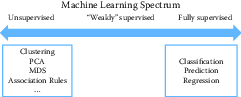
\includegraphics[width=0.7\linewidth]{ChapterML/figures/spectrum} 

}

\caption{Spectrum of machine learning methods from unsupervised to supervised learning}\label{fig:spectrum}
\end{figure}

\section{Methods}\label{methods}

We will start by describing unsupervised learning methods and then go on
to supervised learning methods. We focus here on the intuition behind
the methods and the algorithm, as well as practical tips, rather than on
the statistical theory that underlies the methods. We encourage readers
to refer to machine learning books listed in
Section~\protect\hyperlink{ml:res}{Resources}. Box 6.2 gives brief
definitions of several terms we will use in this section.

\begin{F00}
\textbf{Box 6.2: Machine learning vocabulary}

\begin{itemize}
\item
  \textbf{Learning}: In machine learning, you will notice the term
  \emph{learning} that will be used in the context of ``learning'' a
  model. This is what you probably know as \emph{fitting} or
  \emph{estimating} a function, or \emph{training} or \emph{building} a
  model. These terms are all synonyms and are used interchangeably in
  the machine learning literature.
\item
  \textbf{Examples}: These are data points and instances.
\item
  \textbf{Features}: These are independent variables, attributes,
  predictor variables, and explanatory variables.
\item
  \textbf{Labels}: These include the response variable, dependent
  variable, and target variable.
\item
  \textbf{Underfitting}: This happens when a model is too simple and
  does not capture the structure of the data well enough.
\item
  \textbf{Overfitting}: This happens when a model is possibly too
  complex and models the noise in the data, which can result in poor
  generalization performance. Using in-sample measures to do model
  selection can result in that.
\item
  \textbf{Regularization}: This is a general method to avoid overfitting
  by applying additional constraints to the model that is learned. A
  common approach is to make sure the model weights are, on average,
  small in magnitude. Two common regularizations are \(L_1\)
  regularization (used by the lasso), which has a penalty term that
  encourages the sum of the absolute values of the parameters to be
  small; and \(L_2\) regularization, which encourages the sum of the
  squares of the parameters to be small.
\end{itemize}
\end{F00}

\subsection{Unsupervised learning
methods}\label{unsupervised-learning-methods}

As mentioned earlier, unsupervised learning methods are used when we do
not have a target variable to predict but want to understand ``natural''
clusters or patterns in the data. These methods are often used for
initial data exploration, as in the following examples:

\begin{enumerate}
\def\labelenumi{\arabic{enumi}.}
\item
  When faced with a large corpus of text data---for example, email
  records, congressional bills, speeches, or open-ended free-text survey
  responses---unsupervised learning methods are often used to understand
  and get a handle on what the data contain.
\item
  Given a data set about students and their behavior over time (academic
  performance, grades, test scores, attendance, etc.), one might want to
  understand typical behaviors as well as trajectories of these
  behaviors over time. Unsupervised learning methods (clustering) can be
  applied to these data to get student ``segments'' with similar
  behavior.
\item
  Given a data set about publications or patents in different fields, we
  can use unsupervised learning methods (association rules) to figure
  out which disciplines have the most collaboration and which fields
  have researchers who tend to publish across different fields.
\end{enumerate}

\textbf{Clustering}

Clustering is the most common unsupervised learning technique and is
used to group data points together that are similar to each other. The
goal of clustering methods is to produce with high intra-cluster
(within) similarity and low inter-cluster (between) similarity.

Clustering algorithms typically require a distance (or similarity)
metric\footnote{Distance metrics are mathematical formulas to calculate
  the distance between two objects. For example, \emph{Manhattan
  distance} is the distance a car would drive from one place to another
  place in a grid-based street system, whereas \emph{Euclidian distance}
  (in two-dimensional space) is the ``straight-line'' distance between
  two points.} to generate clusters. They take a data set and a distance
metric (and sometimes additional parameters), and they generate clusters
based on that distance metric. The most common distance metric used is
Euclidean distance, but other commonly used metrics are Manhattan,
Minkowski, Chebyshev, cosine, Hamming, Pearson, and Mahalanobis. Often,
domain-specific similarity metrics can be designed for use in specific
problems. For example, when performing the record linkage tasks
discussed in Chapter~\protect\hyperlink{chap:link}{Record Linkage}, you
can design a similarity metric that compares two first names and assigns
them a high similarity (low distance) if they both map to the same
canonical name, so that, for example, Sammy and Sam map to Samuel.

Most clustering algorithms also require the user to specify the number
of clusters (or some other parameter that indirectly determines the
number of clusters) in advance as a parameter. This is often difficult
to do a priori and typically makes clustering an iterative and
interactive task. Another aspect of clustering that makes it interactive
is often the difficulty in automatically evaluating the quality of the
clusters. While various analytical clustering metrics have been
developed, the best clustering is task-dependent and thus must be
evaluated by the user. There may be different clusterings that can be
generated with the same data. You can imagine clustering similar news
stories based on the topic content, based on the writing style or based
on sentiment. The right set of clusters depends on the user and the task
they have. Clustering is therefore typically used for exploring the
data, generating clusters, exploring the clusters, and then rerunning
the clustering method with different parameters or modifying the
clusters (by splitting or merging the previous set of clusters).
Interpreting a cluster can be nontrivial: you can look at the centroid
of a cluster, look at frequency distributions of different features (and
compare them to the prior distribution of each feature), or you can
build a decision tree (a supervised learning method we will cover later
in this chapter) where the target variable is the cluster ID that can
describe the cluster using the features in your data. A good example of
a tool that allows interactive clustering from text data is Ontogen
(Fortuna, Grobelnik, and Mladenic
\protect\hyperlink{ref-Ontogen}{2007}).

\enlargethispage{6pt} \textbf{\(k\)-means clustering}

The most commonly used clustering algorithm is called \(k\)-means, where
\(k\) defines the number of clusters. The algorithm works as follows:

\begin{enumerate}
\def\labelenumi{\arabic{enumi}.}
\item
  Select \(k\) (the number of clusters you want to generate).
\item
  Initialize by selecting \(k\) points as centroids of the \(k\)
  clusters. This is typically done by selecting \(k\) points uniformly
  at random.
\item
  Assign each point a cluster according to the nearest centroid.
\item
  Recalculate cluster centroids based on the assignment in (3) as the
  mean of all data points belonging to that cluster.
\item
  Repeat (3) and (4) until convergence.
\end{enumerate}

The algorithm stops when the assignments do not change from one
iteration to the next (Figure \ref{fig:kmeans}). The final set of
clusters, however, depend on the starting points. If they are
initialized differently, it is possible that different clusters are
obtained. One common practical trick is to run \(k\)-means several
times, each with different (random) starting points. The \(k\)-means
algorithm is fast, simple, and easy to use, and is often a good first
clustering algorithm to try and see if it fits your needs. When the data
are of the form where the mean of the data points cannot be computed, a
related method called \(K\)-medoids can be used (Park and Jun
\protect\hyperlink{ref-park2009simple}{2009}).

\begin{figure}

{\centering 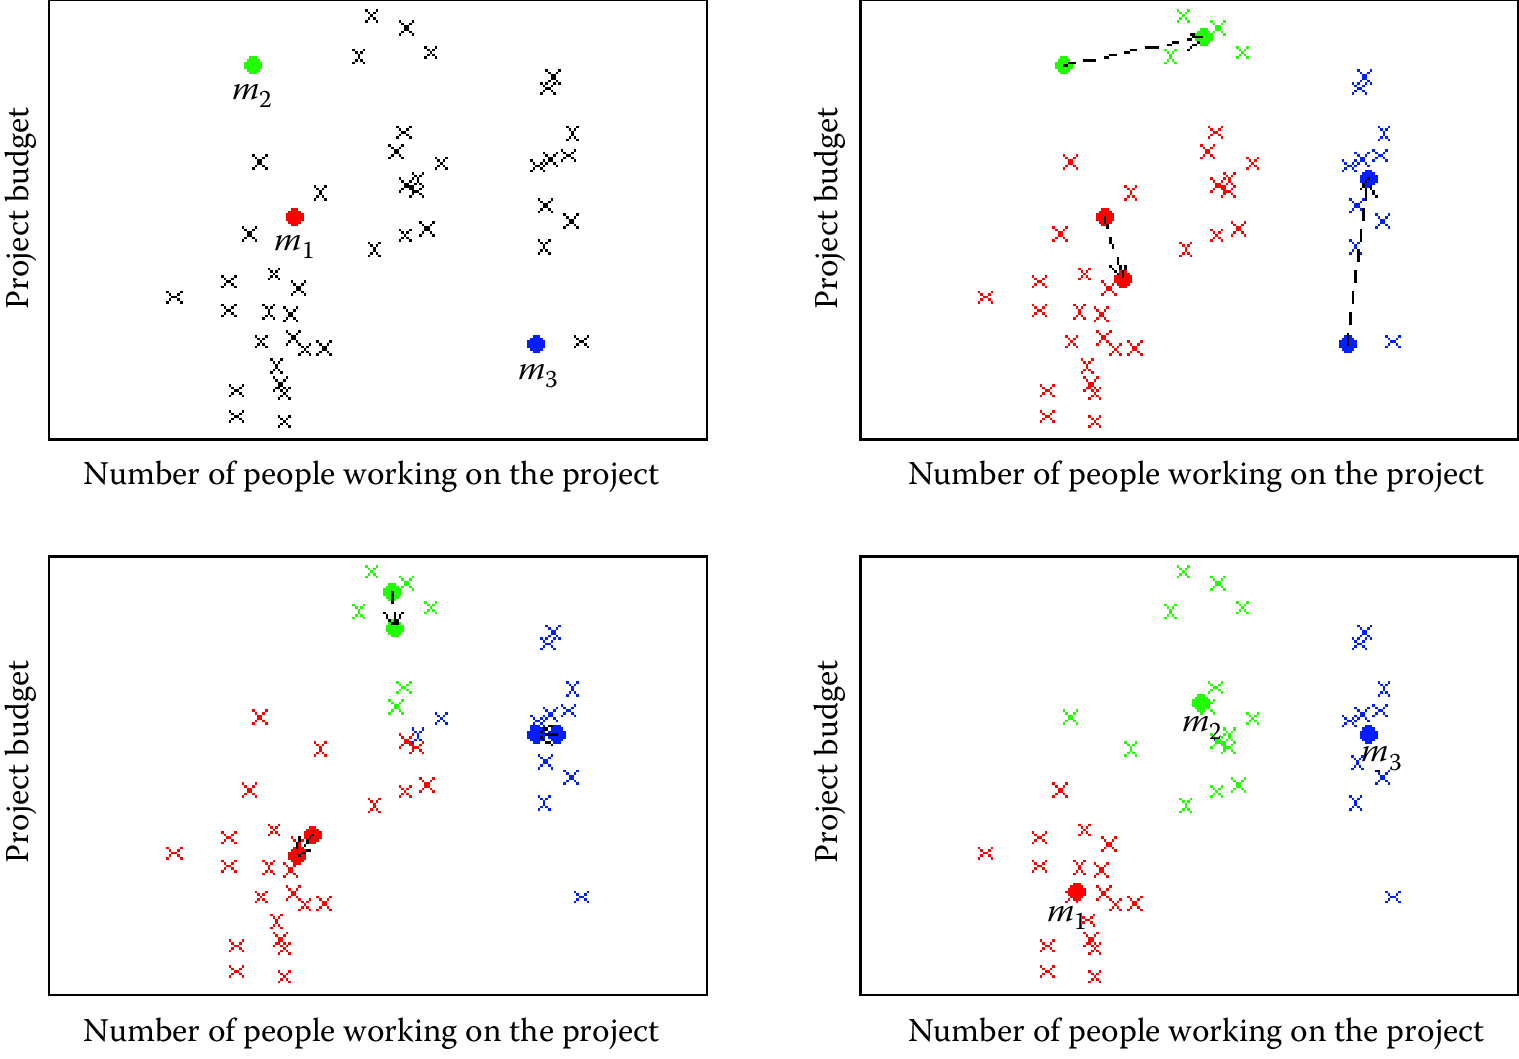
\includegraphics[width=0.7\linewidth]{ChapterML/figures/kmeans} 

}

\caption{Example of $k$-means clustering with $k = 3$. The upper left panel shows the distribution of the data and the three starting points $m_1$, $m_2$, $m_3$ placed at random. On the upper right we see what happens in the first iteration. The cluster means move to more central positions in their respective clusters. The lower left panel shows the second iteration. After six iterations the cluster means have converged to their final destinations and the result is shown in the lower right panel}\label{fig:kmeans}
\end{figure}

\textbf{Expectation-maximization (EM) clustering}

\hspace*{3pt} You may be familiar with the EM algorithm in the context
of imputing missing data. EM is a general approach to maximum likelihood
in the presence of incomplete data. However, it is also used as a
clustering method where the missing data are the clusters a data point
belongs to. Unlike \(k\)-means, where each data point gets assigned to
only one cluster, EM does a soft assignment where each data point gets a
probabilistic assignment to various clusters. The EM algorithm iterates
until the estimates converge to some (locally) optimal solution.

The EM algorithm is fairly good at dealing with outliers as well as
high-dimensional data, compared to \(k\)-means. It also has a few
limitations. First, it does not work well with a large number of
clusters or when a cluster contains few examples. Also, when the value
of \(k\) is larger than the number of actual clusters in the data, EM
may not give reasonable results.

\textbf{Mean shift clustering}

Mean shift clustering works by finding dense regions in the data by
defining a window around each data point and computing the mean of the
data points in the window. Then it shifts the center of the window to
the mean and repeats the algorithm till it converges. After each
iteration, we can consider that the window shifts to a denser region of
the data set. The algorithm proceeds as follows:

\begin{enumerate}
\def\labelenumi{\arabic{enumi}.}
\item
  Fix a window around each data point (based on the bandwidth parameter
  that defines the size of the window).
\item
  Compute the mean of data within the window.
\item
  Shift the window to the mean and repeat till convergence.
\end{enumerate}

Mean shift needs a bandwidth parameter \(h\) to be tuned, which
influences the convergence rate and the number of clusters. A large
\(h\) might result in merging distinct clusters. A small \(h\) might
result in too many clusters. Mean shift might not work well in higher
dimensions since the number of local maxima is pretty high and it might
converge to a local optimum quickly.

One of the most important differences between mean shift and \(k\)-means
is that \(k\)-means makes two broad assumptions: the number of clusters
is already known and the clusters are shaped spherically (or
elliptically). Mean shift does not assume anything about the number of
clusters (but the value of \(h\) indirectly determines that). Also, it
can handle arbitrarily shaped clusters.

The \(k\)-means algorithm is also sensitive to initializations, whereas
mean shift is fairly robust to initializations. Typically, mean shift is
run for each point, or sometimes points are selected uniformly randomly.
Similarly, \(k\)-means is sensitive to outliers, while mean shift is
less sensitive. On the other hand, the benefits of mean shift come at a
cost---speed. The \(k\)-means procedure is fast, whereas classic mean
shift is computationally slow but can be easily parallelized.

\textbf{Hierarchical clustering}

\hspace*{-1pt} The clustering methods that we have seen so far, often
termed \emph{partitioning} methods, produce a flat set of clusters with
no hierarchy. Sometimes, we want to generate a hierarchy of clusters,
and methods that can do that are of two types:

\begin{enumerate}
\def\labelenumi{\arabic{enumi}.}
\item
  \textbf{Agglomerative (bottom-up)}: Start with each point as its own
  cluster and iteratively merge the closest clusters. The iterations
  stop either when the clusters are too far apart to be merged (based on
  a predefined distance criterion) or when there is a sufficient number
  of clusters (based on a predefined threshold).
\item
  \textbf{Divisive (top-down)}: Start with one cluster and create splits
  recursively.
\end{enumerate}

Typically, agglomerative clustering is used more often than divisive
clustering. One reason is that it is significantly faster, although both
of them are typically slower than direct partition methods such as
\(k\)-means and EM. Another disadvantage of these methods is that they
are \emph{greedy}, that is, a data point that is incorrectly assigned to
the ``wrong'' cluster in an earlier split or merge cannot be reassigned
again later on.

\textbf{Spectral clustering}

Figure~\ref{fig:spectral} shows the clusters that \(k\)-means would
generate on the data set in the figure. It is obvious that the clusters
produced are not the clusters you would want, and that is one drawback
of methods such as \(k\)-means. Two points that are far away from each
other will be put in different clusters even if there are other data
points that create a ``path'' between them. Spectral clustering fixes
that problem by clustering data that are connected but not necessarily
(what is called) compact or clustered within convex boundaries. Spectral
clustering methods work by representing data as a graph (or network),
where data points are nodes in the graph and the edges (connections
between nodes) represent the similarity between the two data points.

\begin{figure}

{\centering 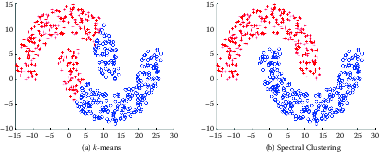
\includegraphics[width=0.7\linewidth]{ChapterML/figures/spectral} 

}

\caption{The same data set can produce drastically different clusters: (a) k-means; (b) spectral clustering}\label{fig:spectral}
\end{figure}

\vspace*{8pt} The algorithm works as follows:

\begin{enumerate}
\def\labelenumi{\arabic{enumi}.}
\item
  Compute a similarity matrix from the data. This involves determining a
  pairwise distance function (using one of the distance functions we
  described earlier).
\item
  With this matrix, we can now perform graph partitioning, where
  connected graph components are interpreted as clusters. The graph must
  be partitioned such that edges connecting different clusters have low
  weights and edges within the same cluster have high values.
\item
  We can now partition these data represented by the similarity matrix
  in a variety of ways. One common way is to use the normalized cuts
  method. Another way is to compute a graph Laplacian from the
  similarity matrix.
\item
  Compute the eigenvectors and eigenvalues of the Laplacian.
\item
  The \(k\) eigenvectors are used as proxy data for the original data
  set, and they are fed into \(k\)-means clustering to produce cluster
  assignments for each original data point.
\end{enumerate}

Spectral clustering is in general much better than \(k\)-means in
clustering performance but much slower to run in practice. For
large-scale problems, \(k\)-means is a preferred clustering algorithm to
run because of efficiency and speed.

\textbf{Principal components analysis}

Principal components analysis is another unsupervised method used for
finding patterns and structure in data. In contrast to clustering
methods, the output is not a set of clusters but a set of
\emph{principal components} that are linear combinations of the original
variables. PCA is typically used when you have a large number of
variables and you want a reduced number that you can analyze. This
approach is often called \emph{dimensionality reduction}. It generates
linearly uncorrelated dimensions that can be used to understand the
underlying structure of the data. In mathematical terms, given a set of
data on \(n\) dimensions, PCA aims to find a linear subspace of
dimension \(d\) lower than \(n\) such that the data points lie mainly on
this linear subspace.

PCA is related to several other methods you may already know about.
Multidimensional scaling, factor analysis, and independent component
analysis differ from PCA in the assumptions they make, but they are
often used for similar purposes of dimensionality reduction and
discovering the underlying structure in a data set.

\textbf{Association rules}

Association rules are a different type of analysis method and originate
from the data mining and database community, primarily focused on
finding frequent co-occurring associations among a collection of items.
This methods is sometimes referred to as ``market basket analysis,''
since that was the original application area of association rules. The
goal is to find associations of items that occur together more often
than you would randomly expect. The classic example (probably a myth) is
``men who go to the store to buy diapers will also tend to buy beer at
the same time.'' This type of analysis would be performed by applying
association rules to a set of supermarket purchase data.

Association rules take the form \(X_1, X_2, X_3 \Rightarrow Y\) with
support \(S\) and confidence \(C\), implying that when a transaction
contains items \(\{X_1, X_2, X_3\}\) \(C\)\% of the time, they also
contain item \(Y\) and there are at least \(S\)\% of transactions where
the antecedent is true. This is useful in cases where we want to find
patterns that are both \emph{frequent} and \emph{statistically
significant}, by specifying thresholds for support \(S\) and confidence
\(C\).

Support and confidence are useful metrics to generate rules but are
often not enough. Another important metric used to generate rules (or
reduce the number of spurious patterns generated) is \emph{lift}. Lift
is simply estimated by the ratio of the joint probability of two items,
\(x\) and \(y\), to the product of their individual probabilities:
\(P(x,y)/[P(x)P(y)]\). If the two items are statistically independent,
then \(P(x,y)=P(x)P(y)\), corresponding to a lift of \(1\). Note that
anti-correlation yields lift values less than 1, which is also an
interesting pattern, corresponding to mutually exclusive items that
rarely occur together.

Association rule algorithms work as follows: Given a set of transactions
(rows) and items for that transaction:

\begin{enumerate}
\def\labelenumi{\arabic{enumi}.}
\item
  Find all combinations of items in a set of transactions that occur
  with a specified minimum frequency. These combinations are called
  \emph{frequent itemsets}.
\item
  Generate association rules that express co-occurrence of items within
  frequent itemsets.
\end{enumerate}

For our purposes, association rule methods are an efficient way to take
a \emph{basket} of features (e.g., areas of publication of a researcher,
different organizations an individual has worked at in their career, all
the cities or neighborhoods someone may have lived in) and find
co-occurrence patterns. This may sound trivial, but as data sets and
number of features get larger, it becomes computationally expensive and
association rule mining algorithms provide a fast and efficient way of
doing it.

\subsection{Supervised learning}\label{sec:MLchapter:super}

We now turn to the problem of supervised learning, which typically
involves methods for classification, prediction, and regression. We will
mostly focus on classification methods in this chapter since many of the
regression methods in machine learning are fairly similar to methods
with which you are already familiar. Remember that classification means
predicting a discrete (or categorical) variable. Some of the
classification methods that we will cover can also be used for
regression, a fact that we will mention when describing that method.

In general, supervised learning methods take as input pairs of data
points \((X,Y)\) where \(X\) are the predictor variables (features) and
\(Y\) is the target variable (label). The supervised learning method
then uses these pairs as \emph{training data} and learns a model \(F\),
where \(F(X)\sim Y\). This model \(F\) is then used to predict \(Y\)s
for new data points \(X\). As mentioned earlier, the goal is not to
build a model that best fits known data but a model that is useful for
future predictions and minimizes future generalization error. This is
the key goal that differentiates many of the methods that you know from
the methods that we will describe next. In order to minimize future
error, we want to build models that are not just \emph{overfitting} on
past data.

Another goal, often prioritized in the social sciences, that machine
learning methods do not optimize for is getting a structural form of the
model. Machine learning models for classification can take different
structural forms (ranging from linear models, to sets of rules, to more
complex forms), and it may not always be possible to write them down in
a compact form as an equation. This does not, however, make them
incomprehensible or uninterpretable. Another focus of machine learning
models for supervised learning is prediction, and not causal
inference\footnote{The topic of causal inference is addressed in more
  detail in Chapter 10.}. Some of these models can be used to help with
causal inference, but they are typically optimized for prediction tasks.
We believe that there are many social science and policy problems where
better prediction methods can be extremely beneficial.

In this chapter, we mostly deal with binary classification problems:
that is, problems in which the data points are to be classified into one
of two categories. Several of the methods that we will cover can also be
used for multiclass classification (classifying a data point into one of
\(n\) categories) or for multi-label classification (classifying a data
point into \(m\) of \(n\) categories where \(m\ge1\)). There are also
approaches to take multiclass problems and turn them into a set of
binary problems that we will mention briefly at the end of the chapter.

Before we describe supervised learning methods, we want to recap a few
principles as well as terms that we have used and will be using in the
rest of the chapter.

\textbf{Training a model}

Once we have finished data exploration, filled in missing values,
created predictor variables (features), and decided what our target
variable (label) is, we now have pairs of \(X,Y\) to start training (or
building) the model.

\textbf{Using the model to score new data}

We are building this model so we can predict \(Y\) for a new set of
\(X\)s---using the model means, getting new data, generating the same
features to get the vector \(X\), and then applying the model to produce
\(Y\).

One common technique for supervised learning is logistic regression, a
method you will already be familiar with. We will give an overview of
some of the other methods used in machine learning. It is important to
remember that as you use increasingly powerful classification methods,
you need more data to \emph{train} the models.

\textbf{\(k\)-nearest neighbor}

The method \(k\)-nearest neighbor (\(k\)-NN) is one of the simpler
classification methods in machine learning. It belongs to a family of
models sometimes known as \emph{memory-based models} or
\emph{instance-based models}. An example is classified by finding its
\(k\) nearest neighbors and taking majority vote (or some other
aggregation function). We need two key things: a value for \(k\) and a
distance metric with which to find the \(k\) nearest neighbors.
Typically, different values of \(k\) are used to empirically find the
best one. Small values of \(k\) lead to predictions having high variance
but can capture the local structure of the data. Larger values of \(k\)
build more global models that are lower in variance but may not capture
local structure in the data as well.

Figure~\ref{fig:knn} provides an example for \(k = 1, 3, 5\) nearest
neighbors. The number of neighbors (\(k\)) is a parameter, and the
prediction depends heavily on how it is determined. In this example,
point B is classified differently if \(k = 3\).

\begin{figure}

{\centering 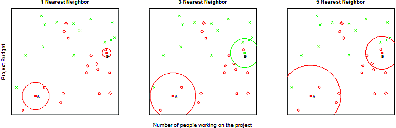
\includegraphics[width=0.7\linewidth]{ChapterML/figures/knn} 

}

\caption{Example of $k$-nearest neighbor with $k = 1, 3, 5$ neighbors. We want to predict the points A and B. The 1-nearest neighbor for both points is red ("Patent not granted"), the 3-nearest neighbor predicts point A (B) to be red (green) with probability 2/3, and the 5-nearest neighbor predicts again both points to be red with probabilities 4/5 and 3/5, respectively.}\label{fig:knn}
\end{figure}

\vspace*{-6pt} Training for \(k\)-NN just means storing the data, making
this method useful in applications where data are coming in extremely
quickly and a model needs to be updated frequently. All the work,
however, gets pushed to scoring time, since all the distance
calculations happen when a new data point needs to be classified. There
are several optimized methods designed to make \(k\)-NN more efficient
that are worth looking into if that is a situation that is applicable to
your problem.

In addition to selecting \(k\) and an appropriate distance metric, we
also have to be careful about the scaling of the features. When
distances between two data points are large for one feature and small
for a different feature, the method will rely almost exclusively on the
first feature to find the closest points. The smaller distances on the
second feature are nearly irrelevant to calculate the overall distance.
A similar problem occurs when continuous and categorical predictors are
used together. To resolve the scaling issues, various options for
rescaling exist. For example, a common approach is to center all
features at mean \(0\) and scale them to variance \(1\).

There are several variations of \(k\)-NN. One of these is weighted
nearest neighbors, where different features are weighted differently or
different examples are weighted based on the distance from the example
being classified. The method \(k\)-NN also has issues when the data are
sparse and has high dimensionality, which means that every point is far
away from virtually every other point, and hence pairwise distances tend
to be uninformative. This can also happen when a lot of features are
irrelevant and drown out the relevant features' signal in the distance
calculations.

Notice that the nearest-neighbor method can easily be applied to
regression problems with a real-valued target variable. In fact, the
method is completely oblivious to the type of target variable and can
potentially be used to predict text documents, images, and videos, based
on the aggregation function after the nearest neighbors are found.

\vspace*{-4pt} \textbf{Support vector machines}

Support vector machines are one of the most popular and best-performing
classification methods in machine learning today. The mathematics behind
SVMs has a lot of prerequisites that are beyond the scope of this book,
but we will give you an intuition of how SVMs work, what they are good
for, and how to use them.

We are all familiar with linear models that separate two classes by
fitting a line in two dimensions (or a hyperplane in higher dimensions)
in the middle (see Figure~\ref{fig:svm}). An important decision that
linear models have to make is which linear separator we should prefer
when there are several we can build.

\begin{figure}

{\centering 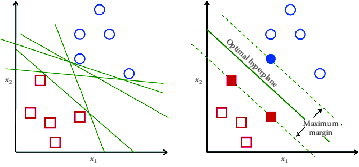
\includegraphics[width=1\linewidth]{ChapterML/figures/svm} 

}

\caption{Support vector machines}\label{fig:svm}
\end{figure}

You can see in Figure~\ref{fig:svm} that multiple lines offer a solution
to the problem. Is any of them better than the others? We can
intuitively define a criterion to estimate the worth of the lines: A
line is bad if it passes too close to the points because it will be
noise sensitive and it will not generalize correctly. Therefore, our
goal should be to find the line passing as far as possible from all
points.

The SVM algorithm is based on finding the hyperplane that maximizes the
\emph{margin} of the training data. The training examples that are
closest to the hyperplane are called \emph{support vectors} since they
are \emph{supporting} the margin (as the margin is only a function of
the support vectors).

An important concept to learn when working with SVMs is \emph{kernels}.
SVMs are a specific instance of a class of methods called \emph{kernel
methods}. So far, we have only talked about SVMs as linear models.
Linear works well in high-dimensional data but sometimes you need
nonlinear models, often in cases of low-dimensional data or in image or
video data. Unfortunately, traditional ways of generating nonlinear
models get computationally expensive since you have to explicitly
generate all the features such as squares, cubes, and all the
interactions. Kernels are a way to keep the efficiency of the linear
machinery but still build models that can capture nonlinearity in the
data without creating all the nonlinear features.

You can essentially think of kernels as similarity functions and use
them to create a linear separation of the data by (implicitly) mapping
the data to a higher-dimensional space. Essentially, we take an
\(n\)-dimensional input vector \(X\), map it into a high-dimensional (
infinite-dimensional) feature space, and construct an optimal separating
hyperplane in this space. We refer you to relevant papers for more
detail on SVMs and nonlinear kernels (Shawe-Taylor and Cristianini
\protect\hyperlink{ref-ShaweTaylor2004}{2004}; Scholkopf and Smola
\protect\hyperlink{ref-Scholkopf2001}{2001}). SVMs are also related to
logistic regression, but use a different loss/penalty function (Hastie,
Tibshirani, and Friedman
\protect\hyperlink{ref-HastieTibshirani}{2001}).

When using SVMs, there are several parameters you have to optimize,
ranging from the \emph{regularization} parameter \(C\), which determines
the tradeoff between minimizing the training error and minimizing model
complexity, to more kernel-specific parameters. It is often a good idea
to do a grid search to find the optimal parameters. Another tip when
using SVMs is to normalize the features; one common approach to doing
that is to normalize each data point to be a vector of unit length.

Linear SVMs are effective in high-dimensional spaces, especially when
the space is sparse such as text classification where the number of data
points (perhaps tens of thousands) is often much less than the number of
features (a hundred thousand to a million or more). SVMs are also fairly
robust when the number of irrelevant features is large (unlike the
\(k\)-NN approaches that we mentioned earlier) as well as when the class
distribution is skewed, that is, when the class of interest is
significantly less than 50\% of the data.

One disadvantage of SVMs is that they do not directly provide
probability estimates. They assign a score based on the distance from
the margin. The farther a point is from the margin, the higher the
magnitude of the score. This score is good for ranking examples, but
getting accurate probability estimates takes more work and requires more
labeled data to be used to perform probability calibrations.

In addition to classification, there are also variations of SVMs that
can be used for regression (Smola and Schölkopf
\protect\hyperlink{ref-SmolaRegression04}{2004}) and ranking (Chapelle
and Keerthi \protect\hyperlink{ref-Chapelle2010}{2010}).

\textbf{Decision trees}

Decision trees are yet another set of methods that are helpful for
prediction. Typical decision trees learn a set of rules from training
data represented as a tree. An exemplary decision tree is shown in
Figure \ref{fig:tree}. Each level of a tree \emph{splits} the tree to
create a branch using a feature and a value (or range of values). In the
example tree, the first split is made on the feature \emph{number of
visits in the past year} and the value \(4\). The second level of the
tree now has two splits: one using \emph{average length of visit} with
value \(2\) days and the other using the value \(10\) days.

\begin{center}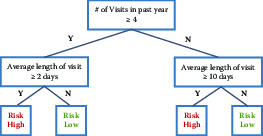
\includegraphics[width=0.7\linewidth]{ChapterML/figures/tree} \end{center}\begin{figure}

{\centering 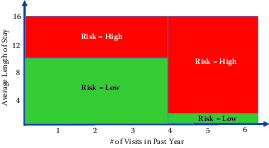
\includegraphics[width=0.7\linewidth]{ChapterML/figures/tree-rectangle} 

}

\caption{An exemplary decision tree. The top figure is the standard representation for trees. The bottom figure offers an alternative view of the same tree. The feature space is partitioned into numerous rectangles, which is another way to view a tree, representing its nonlinear character more explicitly}\label{fig:tree}
\end{figure}

Various algorithms exist to build decision trees. C4.5, CHAID, and CART
(Classification and Regression Trees) are the most Each needs to
determine the next best feature to split on. The goal is to find feature
splits that can best reduce class impurity in the data, that is, a split
that will ideally put all (or as many as possible) positive class
examples on one side and all (or as many as possible) negative examples
on the other side. One common measure of impurity that comes from
information theory is \emph{entropy}, and it is calculated as
\[H(X) = -\sum_x p(x) \log p(x).\]

Entropy is maximum (1) when both classes have equal numbers of examples
in a node. It is minimum (0) when all examples are from the same class.
At each node in the tree, we can evaluate all the possible features and
select the one that most reduces the entropy given the tree so far. This
expected change in entropy is known as \emph{information gain} and is
one of the most common criteria used to create decision trees. Other
measures that are used instead of information gain are Gini and
chi-squared.

If we keep constructing the tree in this manner, selecting the next best
feature to split on, the tree ends up fairly deep and tends to overfit
the data. To prevent overfitting, we can either have a stopping
criterion or \emph{prune} the tree after it is fully grown. Common
stopping criteria include minimum number of data points to have before
doing another feature split, maximum depth, and maximum purity. Typical
pruning approaches use holdout data (or cross-validation, which will be
discussed later in this chapter) to cut off parts of the tree.

Once the tree is built, a new data point is classified by running it
through the tree and, once it reaches a terminal node, using some
aggregation function to give a prediction (classification or
regression). Typical approaches include performing maximum likelihood
(if the leaf node contains 10 examples, 8 positive and 2 negative, any
data point that gets into that node will get an 80\% probability of
being positive). Trees used for regression often build the tree as
described above but then fit a linear regression model at each leaf
node.

Decision trees have several advantages. The interpretation of a tree is
straightforward as long as the tree is not too large. Trees can be
turned into a set of rules that experts in a particular domain can
possibly dig deeper into, validate, and modify. Trees also do not
require too much feature engineering. There is no need to create
interaction terms since trees can implicitly do that by splitting on two
features, one after another.

Unfortunately, along with these benefits come a set of disadvantages.
Decision trees, in general, do not perform well, compared to SVMs,
random forests, or logistic regression. They are also unstable: small
changes in data can result in very different trees. The lack of
stability comes from the fact that small changes in the training data
may lead to different splitting points. As a consequence, the whole tree
may take a different structure. The suboptimal predictive performance
can be seen from the fact that trees partition the predictor space into
a few rectangular regions, each one predicting only a single value (see
the bottom part of Figure \ref{fig:tree}.

\textbf{Ensemble methods}

Combinations of models are generally known as model ensembles. They are
among the most powerful techniques in machine learning, often
outperforming other methods, although at the cost of increased
algorithmic and model complexity.

The intuition behind building ensembles of models is to build several
models, each somewhat different. This diversity can come from various
sources such as: training models on subsets of the data; training models
on subsets of the features; or a combination of these two.

Ensemble methods in machine learning have two things in common. First,
they construct multiple, diverse predictive models from adapted versions
of the training data (most often reweighted or resampled). Second, they
combine the predictions of these models in some way, often by simple
averaging or voting (possibly weighted).

\textbf{Bagging}

Bagging stands for ``bootstrap aggregation''\footnote{Bootstrap is a
  general statistical procedure that draws random samples of the
  original data with replacement.}: we first create bootstrap samples
from the original data and then aggregate the predictions using models
trained on each bootstrap sample. Given a data set of size \(N\), the
method works as follows:

\begin{enumerate}
\def\labelenumi{\arabic{enumi}.}
\item
  Create \(k\) bootstrap samples (with replacement), each of size \(N\),
  resulting in \(k\) data sets. Only about 63\% of the original training
  examples will be represented in any given bootstrapped set.
\item
  Train a model on each of the \(k\) data sets, resulting in \(k\)
  models.
\item
  For a new data point \(X\), predict the output using each of the \(k\)
  models.
\item
  Aggregate the \(k\) predictions (typically using average or voting) to
  get the prediction for \(X\).
\end{enumerate}

A nice feature of this method is that any underlying model can be used,
but decision trees are often the most commonly used base model. One
reason for this is that decision tress are typically high variance and
unstable, that is, they can change drastically given small changes in
data, and bagging is effective at reducing the variance of the overall
model. Another advantage of bagging is that each model can be trained in
parallel, making it efficient to scale to large data sets.

\textbf{Boosting}

Boosting is another popular ensemble technique, and it often results in
improving the base classifier being used. In fact, if your only goal is
improving accuracy, you will most likely find that boosting will achieve
that. The basic idea is to keep training classifiers iteratively, each
iteration focusing on examples that the previous one got wrong. At the
end, you have a set of classifiers, each trained on smaller and smaller
subsets of the training data. Given a new data point, all the
classifiers predict the target, and a weighted average of those
predictions is used to get the final prediction, where the weight is
proportional to the accuracy of each classifier. The algorithm works as
follows:

\begin{enumerate}
\def\labelenumi{\arabic{enumi}.}
\item
  Assign equal weights to every example.
\item
  For each iteration:

  \begin{enumerate}
  \def\labelenumii{\arabic{enumii}.}
  \item
    Train classifier on the weighted examples.
  \item
    Predict on the training data.
  \item
    Calculate error of the classifier on the training data.
  \item
    Calculate the new weighting on the examples based on the errors of
    the classifier.
  \item
    Reweight examples.
  \end{enumerate}
\item
  Generate a weighted classifier based on the accuracy of each
  classifier.
\end{enumerate}

One constraint on the classifier used within boosting is that it should
be able to handle weighted examples (either directly or by replicating
the examples that need to be overweighted). The most common classifiers
used in boosting are decision stumps (single-level decision trees), but
deeper trees can also work well.

Boosting is a common way to \emph{boost} the performance of a
classification method but comes with additional complexity, both in the
training time and in interpreting the predictions. A disadvantage of
boosting is that it is difficult to parallelize since the next iteration
of boosting relies on the results of the previous iteration.

A nice property of boosting is its ability to identify outliers:
examples that are either mislabeled in the training data, or are
inherently ambiguous and hard to categorize. Because boosting focuses
its weight on the examples that are more difficult to classify, the
examples with the highest weight often turn out to be outliers. On the
other hand, if the number of outliers is large (lots of noise in the
data), these examples can hurt the performance of boosting by focusing
too much on them.

\textbf{Random forests}

Given a data set of size \(N\) and containing \(M\) features, the random
forest training algorithm works as follows:

\begin{enumerate}
\def\labelenumi{\arabic{enumi}.}
\item
  Create \(n\) bootstrap samples from the original data of size \(N\).
  Remember, this is similar to the first step in bagging. Typically
  \(n\) ranges from 100 to a few thousand but is best determined
  empirically.
\item
  For each bootstrap sample, train a decision tree using \(m\) features
  (where \(m\) is typically much smaller than \(M\)) at each node of the
  tree. The \(m\) features are selected uniformly at random from the
  \(M\) features in the data set, and the decision tree will select the
  best split among the \(m\) features. The value of \(m\) is held
  constant during the forest growing.
\item
  A new test example/data point is classified by all the trees, and the
  final classification is done by majority vote (or another appropriate
  aggregation method).
\end{enumerate}

Random forests are probably the most accurate classifiers being used
today in machine learning. They can be easily parallelized, making them
efficient to run on large data sets, and can handle a large number of
features, even with a lot of missing values. Random forests can get
complex, with hundreds or thousands of trees that are fairly deep, so it
is difficult to interpret the learned model. At the same time, they
provide a nice way to estimate feature importance, giving a sense of
what features were important in building the classifier.

Another nice aspect of random forests is the ability to compute a
proximity matrix that gives the similarity between every pair of data
points. This is calculated by computing the number of times two examples
land in the same terminal node. The more that happens, the closer the
two examples are. We can use this proximity matrix for clustering,
locating outliers, or explaining the predictions for a specific example.

\textbf{Stacking}

Stacking is a technique that deals with the task of learning a
meta-level classifier to combine the predictions of multiple base-level
classifiers. This meta-algorithm is trained to combine the model
predictions to form a final set of predictions. This can be used for
both regression and classification. The algorithm works as follows:

\begin{enumerate}
\def\labelenumi{\arabic{enumi}.}
\item
  Split the data set into \(n\) equal-sized sets:
  \(set_1, set_2,\ldots,set_n\).
\item
  Train base models on all possible combinations of \(n-1\) sets and,
  for each model, use it to predict on \(set_i\) what was left out of
  the training set. This would give us a set of predictions on every
  data point in the original data set.
\item
  Now train a second-stage stacker model on the predicted classes or the
  predicted probability distribution over the classes from the
  first-stage (base) model(s).
\end{enumerate}

By using the first-stage predictions as features, a stacker model gets
more information on the problem space than if it were trained in
isolation. The technique is similar to cross-validation, an evaluation
methodology that we will cover later in this chapter.

\textbf{Neural networks and deep learning}

Neural networks are a set of multi-layer classifiers where the outputs
of one layer feed into the inputs of the next layer. The layers between
the input and output layers are called \emph{hidden layers}, and the
more hidden layers a neural network has, the more complex functions it
can learn. Neural networks were popular in the 1980s and early 1990s,
but then fell out of fashion because they were slow and expensive to
train, even with only one or two hidden layers. Since 2006, a set of
techniques has been developed that enable learning in deeper neural
networks. These techniques have enabled much deeper (and larger)
networks to be trained---people now routinely train networks with five
to ten hidden layers. And it turns out that these perform far better on
many problems than shallow neural networks (with just a single hidden
layer). The reason for the better performance is the ability of deep
nets to build up a complex hierarchy of concepts, learning multiple
levels of representation and abstraction that help to make sense of data
such as images, sound, and text.

Usually, with a supervised neural network you try to predict a target
vector, \(Y\), from a matrix of inputs, \(X\). But when you train a deep
neural network, it uses a combination of supervised and unsupervised
learning. In an unsupervised neural network, you try to predict the
matrix \(X\) using the same matrix \(X\) as the input. In doing this,
the network can learn something intrinsic about the data without the
help of a separate target or label. The learned information is stored as
the weights of the network.

Currently, deep neural networks are trendy and a lot of research is
being done on them. It is, however, important to keep in mind that they
are applicable for a narrow class of problems with which social
scientists would deal and that they often require a lot more data than
are available in most problems. Training deep neural networks also
requires a lot of computational power, but that is less likely to be an
issue for most people. Typical cases where deep learning has been shown
to be effective involve lots of images, video, and text data. We are
still in the early stages of development of this class of methods, and
the next few years will give us a much better understanding of why they
are effective and the problems for which they are well suited.

\section{Evaluation}\label{evaluation}

The previous section introduced us to a variety of methods, all with
certain pros and cons, and no single method guaranteed to outperforms
others for a given problem. This section focuses on evaluation methods,
with three primary goals:

\begin{enumerate}
\def\labelenumi{\arabic{enumi}.}
\item
  Model selection: How do we select a method to use? What parameters
  should we select for that method?
\item
  Performance estimation: How well will our model do once it is deployed
  and applied to new data?
\item
  A deeper understanding of the model can point to inaccuracies of
  existing methods and provide a better understanding of the data and
  the problem we are tackling.
\end{enumerate}

This section will cover evaluation methodologies as well as metrics that
are commonly used. We will start by describing common evaluation
methodologies that use existing data and then move on to field trials.
The methodologies we describe below apply both to regression and
classification problems.

\subsection{Methodology}\label{methodology}

\textbf{In-sample evaluation}

As social scientists, you already evaluate methods on how well they
perform in-sample (on the set that the model was trained on). As we
mentioned earlier in the chapter, the goal of machine learning methods
is to generalize to new data, and validating models in-sample does not
allow us to do that. We focus here on evaluation methodologies that
allow us to optimize (as best as we can) for generalization performance.
The methods are illustrated in Figure~\ref{fig:holdout}.

\textbf{Out-of-sample and holdout set}

The simplest way to focus on generalization is to \emph{pretend} to
generalize to new (unseen) data. One way to do that is to take the
original data and randomly split them into two sets: a \emph{training
set} and a \emph{test set} (sometimes also called the \emph{holdout} or
\emph{validation set}). We can decide how much to keep in each set
(typically the splits range from 50--50 to 80--20, depending on the size
of the data set). We then train our models on the training set and
classify the data in the test set, allowing us to get an estimate of the
relative performance of the methods.

One drawback of this approach is that we may be extremely lucky or
unlucky with our random split. One way to get around the problem that is
to repeatedly create multiple training and test sets. We can then train
on \(TR_1\) and test on \(TE_1\), train on \(TR_2\) and test on
\(TE_2\), and so on. The performance measures on each test set can then
give us an estimate of the performance of different methods and how much
they vary across different random sets.

\begin{figure}

{\centering 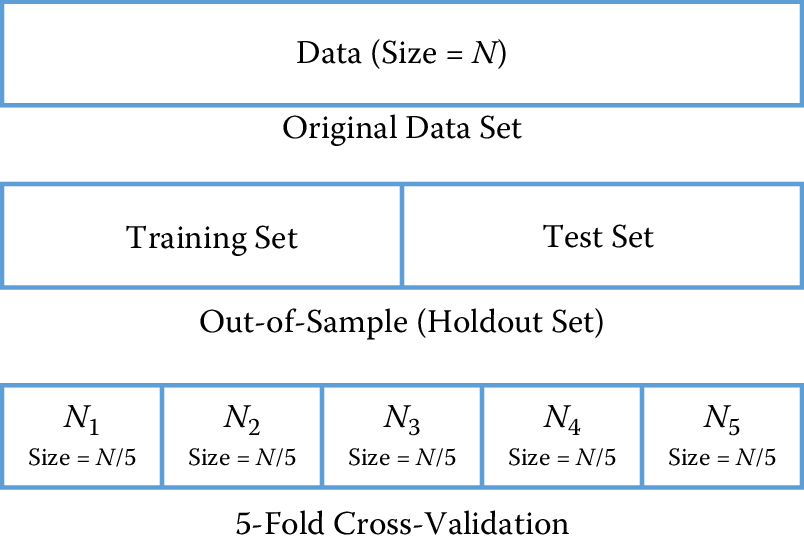
\includegraphics[width=0.7\linewidth]{ChapterML/figures/holdout} 

}

\caption{Validation methodologies: holdout set and cross-validation}\label{fig:holdout}
\end{figure}

\textbf{Cross-validation}

Cross-validation is a more sophisticated holdout training and testing
procedure that takes away some of the shortcomings of the holdout set
approach. Cross-validation begins by splitting a labeled data set into
\(k\) partitions (called folds). Typically, \(k\) is set to \(5\) or
\(10\). Cross-validation then proceeds by iterating \(k\) times. In each
iteration, one of the \(k\) folds is held out as the test set, while the
other \(k-1\) folds are combined and used to train the model. A nice
property of cross-validation is that every example is used in one test
set for testing the model. Each iteration of cross-validation gives us a
performance estimate that can then be aggregated (typically averaged) to
generate the overall estimate.

An extreme case of cross-validation is called leave-one-out
cross-validation, where given a data set of size \(N\), we create \(N\)
folds. That means iterating over each data point, holding it out as the
test set, and training on the rest of the \(N-1\) examples. This
illustrates the benefit of cross-validation by giving us good
generalization estimates (by training on as much of the data set as
possible) and making sure the model is tested on each data point.

\textbf{Temporal validation}

\hspace*{4pt} The cross-validation and holdout set approaches described
above assume that the data have no time dependencies and that the
distribution is stationary over time. This assumption is almost always
violated in practice and affects performance estimates for a model.

\begin{figure}

{\centering 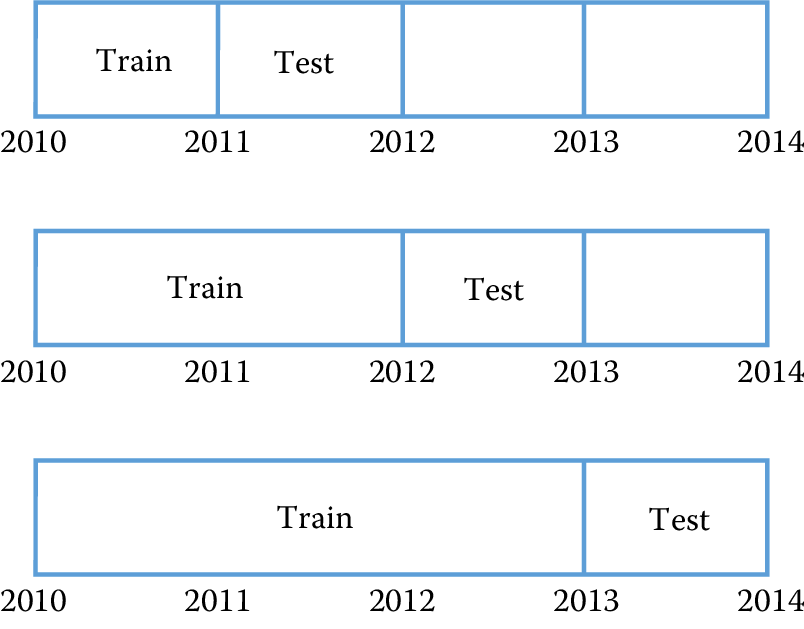
\includegraphics[width=0.7\linewidth]{ChapterML/figures/temporal} 

}

\caption{Temporal validation}\label{fig:temporal}
\end{figure}

In most practical problems, we want to use a validation strategy that
emulates the way in which our models will be used and provides an
accurate performance estimate. We will call this \emph{temporal
validation}. For a given point in time \(t_i\), we train our models only
on information available to us before \(t_i\) to avoid training on data
from the ``future.'' We then predict and evaluate on data from \(t_i\)
to \(t_i\) + \(d\) and iterate, expanding the training window while
keeping the test window size constant at \(d\).
Figure~\ref{fig:temporal} shows this validation process with
\(t_i=2010\) and \(d=1\) year. The test set window \(d\) depends on a
few factors related to how the model will be deployed to best emulate
reality:

\begin{enumerate}
\def\labelenumi{\arabic{enumi}.}
\item
  How far out in the future do predictions need to be made? For example,
  if the set of students who need to be targeted for interventions has
  to be finalized at the beginning of the school year for the entire
  year, then \(d = 1\) year.
\item
  How often will the model be updated? If the model is being updated
  daily, then we can move the window by a day at a time to reflect the
  deployment scenario.
\item
  How often will the system get new data? If we are getting new data
  frequently, we can make predictions more frequently.
\end{enumerate}

Temporal validation is similar to how time series models are evaluated
and should be the validation approach used for most practical problems.

\subsection{Metrics}\label{metrics}

The previous subsection focused on validation methodologies assuming we
have a evaluation metric in mind. This section will go over commonly
used evaluation metrics. You are probably familiar with using \(R^2\),
analysis of the residuals, and mean squared error (MSE) to evaluate the
quality of regression models. For regression problems, the MSE
calculates the average squared differences between predictions
\(\hat{y}_i\) and true values \(y_i\). When prediction models have
smaller MSE, they are better. However, the MSE itself is hard to
interpret because it measures quadratic differences. Instead, the root
mean squared error (RMSE) is more intuitive as it as measure of mean
differences on the original scale of the response variable. Yet another
alternative is the mean absolute error (MAE), which measures average
absolute distances between predictions and true values.

We will now describe some additional evaluation metrics commonly used in
machine learning for classification. Before we dive into metrics, it is
important to highlight that machine learning models for classification
typically do not predict 0/1 values directly. SVMs, random forests, and
logistic regression all produce a score (which is sometimes a
probability) that is then turned into 0 or 1 based on a user-specific
threshold. You might find that certain tools (such as ) use a default
value for that threshold (often 0.5), but it is important to know that
it is an arbitrary threshold and you should select the threshold based
on the data, the model, and the problem you are solving. We will cover
that a little later in this section.

Once we have turned the real-valued predictions into 0/1 classification,
we can now create a \emph{confusion matrix} from these predictions,
shown in Figure \ref{fig:cm}. Each data point belongs to either the
positive class or the negative class, and for each data point the
prediction of the classifier is either correct or incorrect. This is
what the four cells of the confusion matrix represent. We can use the
confusion matrix to describe several commonly used evaluation metrics.

\begin{figure}

{\centering 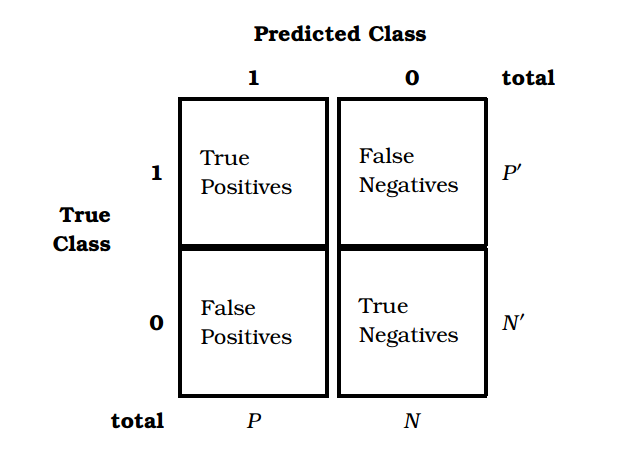
\includegraphics[width=0.7\linewidth]{ChapterML/figures/cm} 

}

\caption{A *confusion matrix* created from real-valued predictions}\label{fig:cm}
\end{figure}

Accuracy is the ratio of correct predictions (both positive and
negative) to all predictions:
\[\textrm{Accuracy}=\frac{TP + TN}{TP + TN + FP + FN}=\frac{TP + TN}{P+N}=\frac{TP + TN}{P'+N'},\]
where \(TP\) denotes true positives, \(TN\) true negatives, \(FP\) false
positives, \(FN\) false negatives, and other symbols denote row or
column totals as in Figure~. Accuracy is the most commonly described
evaluation metric for classification but is surprisingly the least
useful in practical situations (at least by itself). One problem with
accuracy is that it does not give us an idea of \emph{lift} compared to
baseline. For example, if we have a classification problem with 95\% of
the data as positive and 5\% as negative, a classifier with 85\% is
performing worse than a dumb classifier that predicts positive all the
time (and will have 95\% accuracy).

Two additional metrics that are often used are precision and recall,
which are defined as follows: \[\begin{aligned}
{\rm Precision} &= \frac{TP}{TP + FP}=\frac{TP}{P},
\\
{\rm Recall} &= \frac{TP}{TP + FN}=\frac{TP}{P'}\end{aligned}\] (see
also Box 7.3). Precision measures the accuracy of the classifier when it
predicts an example to be positive. It is the ratio of correctly
predicted positive examples (\(TP\)) to all examples predicted as
positive (\(TP + FP\)). This measure is also called \emph{positive
predictive value} in other fields. Recall measures the ability of the
classifier to find positive examples. It is the ratio of all the
correctly predicted positive examples (\(TP\)) to all the positive
examples in the data (\(TP + FN\)). This is also called
\emph{sensitivity} in other fields.

You might have encountered another metric called \emph{specificity} in
other fields. This measure is the true negative rate: the proportion of
negatives that are correctly identified.

Another metric that is used is the \(F_1\) score, which is the harmonic
mean of precision and recall:
\[F_1 =  \frac{2* {\rm Precision} * {\rm Recall}}{{\rm Precision} + {\rm Recall}}\]
(see also equation 7.1). This is often used when you want to balance
both precision and recall.

There is often a tradeoff between precision and recall. By selecting
different classification thresholds, we can vary and tune the precision
and recall of a given classifier. A highly conservative classifier that
only predicts a 1 when it is absolutely sure (say, a threshold of
0.9999) will most often be correct when it predicts a 1 (high precision)
but will miss most 1s (low recall). At the other extreme, a classifier
that says 1 to every data point (a threshold of 0.0001) will have
perfect recall but low precision. Figure~\ref{fig:pr} show a
precision--recall curve that is often used to represent the performance
of a given classifier.

\begin{figure}

{\centering 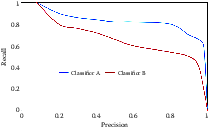
\includegraphics[width=0.7\linewidth]{ChapterML/figures/pr} 

}

\caption{Precision-recall curve}\label{fig:pr}
\end{figure}

\begin{figure}

{\centering 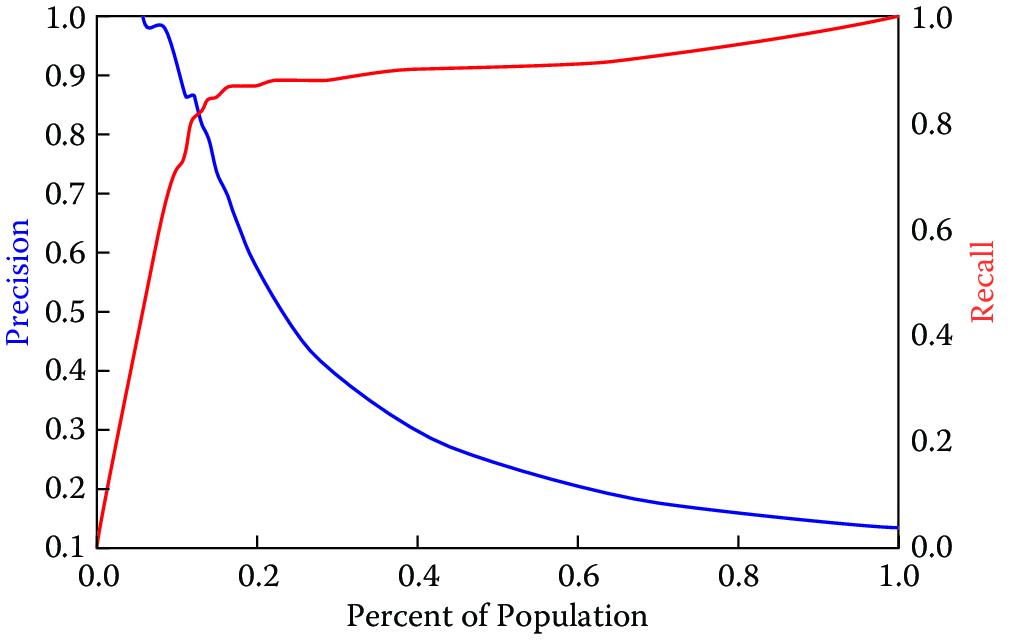
\includegraphics[width=0.7\linewidth]{ChapterML/figures/pr2} 

}

\caption{Precision or recall at different thresholds}\label{fig:pr2}
\end{figure}

If we care about optimizing for the entire precision recall space, a
useful metric is the \emph{area under the curve} (AUC-PR), which is the
area under the precision--recall curve. AUC-PR must not be confused with
AUC-ROC, which is the area under the related receiver operating
characteristic (ROC) curve. The ROC curve is created by plotting recall
versus (1 -- specificity). Both AUCs can be helpful metrics to compare
the performance of different methods and the maximum value the AUC can
take is 1. If, however, we care about a specific part on the
precision--recall curve, we have to look at finer-grainedmetrics.

Let us consider an example from public health. Most public health
agencies conduct inspections of various sorts to detect health hazard
violations (lead hazards, for example). The number of possible places
(homes or businesses) to inspect far exceeds the inspection resources
typically available. Let us assume further that they can only inspect
5\% of all possible places; they would clearly want to prioritize the
inspection of places that are most likely to contain the hazard. In this
case, the model will score and rank all the possible inspection places
in order of hazard risk. We would then want to know what percentage of
the top 5\% (the ones that will get inspected) are likely to be hazards,
which translates to the precision in the top 5\% of the most confidence
predictions---precision at 5\%, as it is commonly called (see Figure
\ref{fig:pr2}). \emph{Precision at top k percent} is a common class of
metrics widely used in information retrieval and search engine
literature, where you want to make sure that the results retrieved at
the top of the search results are accurate. More generally, this metric
is often used in problems in which the class distribution is skewed and
only a small percentage of the examples will be examined manually
(inspections, investigations for fraud, etc.). The literature provides
many case studies of such applications (Kumar, Ghani, and Mei
\protect\hyperlink{ref-Kumar2010}{2010}; Lakkaraju et al.
\protect\hyperlink{ref-Lakkaraju2015}{2015}; Potash et al.
\protect\hyperlink{ref-Potash2015}{2015}).

\enlargethispage{6pt} One last metric we want to mention is a class of
cost-sensitive metrics where different costs (or benefits) can be
associated with the different cells in the confusion matrix. So far, we
have implicitly assumed that every correct prediction and every error,
whether for the positive class or the negative class, has equal costs
and benefits. In many practical problems, that is not the case. For
example, we may want to predict whether a patient in a hospital
emergency room is likely to go into cardiac arrest in the next six
hours. The cost of a false positive in this case is the cost of the
intervention (which may be a few extra minutes of a physician's time)
while the cost of a false negative could be death. This type of analysis
allows us to calculate the expected value of the predictions of a
classifier and select the model that optimizes this cost-sensitive
metric.

\section{Practical tips}\label{practical-tips}

Here we highlight some practical tips that will be helpful when working
with machine learning methods.

\subsection{Features}\label{features}

So far in this chapter, we have focused a lot on methods and process,
and we have not discussed features in detail. In social science, they
are not called features but instead are known as variables or
predictors. {Good features are what makes machine learning systems
effective}. Feature generation (or engineering, as it is often called)
is where the bulk of the time is spent in the machine learning process.
As social science researchers or practitioners, you have spent a lot of
time constructing features, using transformations, dummy variables, and
interaction terms. All of that is still required and critical in the
machine learning framework. One difference you will need to get
comfortable with is that instead of carefully selecting a few
predictors, machine learning systems tend to encourage the creation of
lots of features and then empirically use holdout data to perform
regularization and model selection. It is common to have models that are
trained on thousands of features. Commonly used approaches to create
features include:

\begin{itemize}
\item
  \textbf{Transformations}, such as log, square, and square root.
\item
  \textbf{Dummy (binary) variables}: This is often done by taking
  categorical variables (such as city) and creating a binary variable
  for each value (one variable for each city in the data). These are
  also called indicator variables.
\item
  \textbf{Discretization}: Several methods require features to be
  discrete instead of continuous. Several approaches exist to convert
  continuous variables into discrete ones, the most common of which is
  equal-width binning.
\item
  \textbf{Aggregation}: Aggregate features often constitute the majority
  of features for a given problem. These aggregations use different
  aggregation functions (count, min, max, average, standard deviation,
  etc.), often over varying windows of time and space. For example,
  given urban data, we would want to calculate the number (and min, max,
  mean, variance) of crimes within an \(m\)-mile radius of an address in
  the past \(t\) months for varying values of \(m\) and \(t\), and then
  to use all of them as features in a classification problem.
\end{itemize}

In general, it is a good idea to have the complexity in features and use
a simple model, rather than using more complex models with simple
features. Keeping the model simple makes it faster to train and easier
to understand.

\subsection{Machine learning pipeline}\label{machine-learning-pipeline}

When working on machine learning projects, it is a good idea to
structure your code as a modular pipeline so you can easily try
different approaches and methods without major restructuring. The Python
workbooks supporting this book will give you an example of a machine
learning pipeline. A good pipeline will contain modules for importing
data, doing exploration, feature generation, classification, and
evaluation. You can then instantiate a specific workflow by combining
these modules.

An important component of the machine learning pipeline is comparing
different methods. With all the methods out there and all the
hyperparameters they come with, how do we know which model to use and
which hyperparameters to select? And what happens when we add new
features to the model or when the data have ``temporal drift'' and
change over time? One simple approach is to have a nested set of loops
that loop over all the methods you have access to, then enumerate all
the hyperparameters for that method, create a cross-product, and loop
over all of them, comparing them across different evaluation metrics and
selecting the best one to use going forward. You can even add different
feature subsets and time slices to this loop, as the example in the
supporting workbooks will show.

\subsection{Multiclass problems}\label{multiclass-problems}

In the supervised learning section, we framed classification problems as
binary classification problems with a 0 or 1 output. There are many
problems where we have multiple classes, such as classifying companies
into their industry codes or predicting whether a student will drop out,
transfer, or graduate. Several solutions have been designed to deal with
the multiclass classification problem:

\begin{itemize}
\item
  \textbf{Direct multiclass}: Use methods that can directly perform
  multiclass classification. Examples of such methods are \(K\)-nearest
  neighbor, decision trees, and random forests. There are extensions of
  support vector machines that exist for multiclass classification as
  well (Crammer and Singer \protect\hyperlink{ref-crammer2002}{2002}),
  but they can often be slow to train.
\item
  \textbf{Convert to one versus all (OVA)}: This is a common approach to
  solve multiclass classification problems using binary classifiers. Any
  problem with \(n\) classes can be turned into \(n\) binary
  classification problems, where each classifier is trained to
  distinguish between one versus all the other classes. A new example
  can be classified by combining the predictions from all the \(n\)
  classifiers and selecting the class with the highest score. This is a
  simple and efficient approach, and one that is commonly used, but it
  suffers from each classification problem possibly having an imbalanced
  class distribution (due to the negative class being a collection of
  multiple classes). Another limitation of this approach is that it
  requires the scores of each classifier to be calibrated so that they
  are comparable across all of them.
\item
  \textbf{Convert to pairwise}: In this approach, we can create binary
  classifiers to distinguish between each pair of classes, resulting in
  \(\binom{n}{2}\) binary classifiers. This results in a large number of
  classifiers, but each classifier usually has a balanced classification
  problem. A new example is classified by taking the predictions of all
  the binary classifiers and using majority voting.
\end{itemize}

\subsection{Skewed or imbalanced classification
problems}\label{skewed-or-imbalanced-classification-problems}

A lot of problems you will deal with will not have uniform (balanced)
distributions for both classes. This is often the case with problems in
fraud detection, network security, and medical diagnosis where the class
of interest is not very common. The same is true in many social science
and public policy problems around behavior prediction, such as
predicting which students will not graduate on time, which children may
be at risk of getting lead poisoning, or which homes are likely to be
abandoned in a given city. You will notice that applying standard
machine learning methods may result in all the predictions being for the
most frequent category in such situations, making it problematic to
detect the infrequent classes. There has been a lot of work in machine
learning research on dealing with such problems (Chawla
\protect\hyperlink{ref-Chawla05}{2005}; Kuhn and Johnson
\protect\hyperlink{ref-KuhnJohnson2013}{2013}) that we will not cover in
detail here. Common approaches to deal with class imbalance include
oversampling from the minority class and undersampling from the majority
class. It is important to keep in mind that the sampling approaches do
not need to result in a \(1:1\) ratio. Many supervised learning methods
described in this chapter (such as SVMs) can work well even with a
\(10:1\) imbalance. Also, it is critical to make sure that you only
resample the training set; keep the distribution of the test set the
same as that of the original data since you will not know the class
labels of new data in practice and will not be able to resample.

\section{How can social scientists benefit from machine
learning?}\label{how-can-social-scientists-benefit-from-machine-learning}

In this chapter, we have introduced you to some new methods (both
unsupervised and supervised), validation methodologies, and evaluation
metrics. All of these can benefit social scientists as they tackle
problems in research and practice. In this section, we will give a few
concrete examples where what you have learned so far can be used to
improve some social science tasks:

\begin{itemize}
\item
  \textbf{Use of better prediction methods and methodology}: Traditional
  statistics and social sciences have not focused much on methods for
  prediction. Machine learning researchers have spent the past 30 years
  developing and adapting methods focusing on that task. We believe that
  there is a lot of value for social science researchers and
  practitioners in learning more about those methods, applying them, and
  even augmenting them (Kleinberg et al.
  \protect\hyperlink{ref-Kleinberg2015}{2015}). Two common tasks that
  can be improved using better prediction methods are generating
  counterfactuals (essentially a prediction problem) and matching. In
  addition, holdout sets and cross-validation can be used as a model
  selection methodology with any existing regression and classification
  methods, resulting in improved model selection and error estimates.
\item
  \textbf{Model misspecification}: Linear and logistic regressions are
  common techniques for data analysis in the social sciences. One
  fundamental assumption within both is that they are additive over
  parameters. Machine learning provides tools when this assumption is
  too limiting. Hainmueller and Hazlett (Hainmueller and Hazlett
  \protect\hyperlink{ref-hainmueller2014kernel}{2014}), for example,
  reanalyze data that were originally analyzed with logistic regression
  and come to substantially different conclusions. They argue that their
  analysis, which is more flexible and based on supervised learning
  methodology, provides three additional insights when compared to the
  original model. First, predictive performance is similar or better,
  although they do not need an extensive search to find the final model
  specification as it was done in the original analysis. Second, their
  model allows them to calculate average marginal effects that are
  mostly similar to the original analysis. However, for one covariate
  they find a substantially different result, which is due to model
  misspecification in the original model. Finally, the reanalysis also
  discovers interactions that were missed in the original publication.
\item
  \textbf{Better text analysis}: Text is everywhere, but unfortunately
  humans are slow and expensive in analyzing text data. Thus, computers
  are needed to analyze large collections of text. Machine learning
  methods can help make this process more efficient. Feldman and Sanger
  (Feldman and Sanger \protect\hyperlink{ref-FeldmanSanger}{2006})
  provide an overview of different automatic methods for text analysis.
  Grimmer and Stewart (Grimmer and Stewart
  \protect\hyperlink{ref-grimmer2013text}{2013}) give examples that are
  more specific for social scientists, and
  Chapter~\protect\hyperlink{chap:text}{Text analysis} provides more
  details on this topic.
\item
  \textbf{Adaptive surveys}: Some survey questions have a large number
  of possible answer categories. For example, international job
  classifications describe more than 500 occupational categories, and it
  is prohibitive to ask all categories during the survey. Instead,
  respondents answer an open-ended question about their job and machine
  learning algorithms can use the verbatim answers to suggest small sets
  of plausible answer options. The respondents can then select which
  option is the best description for their occupation, thus saving the
  costs for coding after the interview.
\item
  \textbf{Estimating heterogeneous treatment effects}: A standard
  approach to causal inference is the assignment of different treatments
  (e.g., medicines) to the units of interest (e.g., patients).
  Researchers then usually calculate the average treatmenteffect---the
  average difference in outcomes for both groups. It is also of interest
  if treatment effects differ for various subgroups (e.g., is a medicine
  more effective for younger people?). Traditional subgroup analysis has
  been criticized and challenged by various machine learning techniques
  (Green and Kern \protect\hyperlink{ref-green2012modeling}{2012}; Imai,
  Ratkovic, and others
  \protect\hyperlink{ref-imai2013estimating}{2013}).
\item
  \textbf{Variable selection}: Although there are many methods for
  variable selection, regularized methods such as the lasso are highly
  effective and efficient when faced with large amounts of data. Varian
  (Varian \protect\hyperlink{ref-Varian2014}{2014}) goes into more
  detail and gives other methods from machine learning that can be
  useful for variable selection. We can also find interactions between
  pairs of variables (to feed into other models) using random forests,
  by looking at variables that co-occur in the same tree, and by
  calculating the strength of the interaction as a function of how many
  trees they co-occur in, how high they occur in the trees, and how far
  apart they are in a given tree.
\end{itemize}

\section{Advanced topics}\label{advanced-topics}

This has been a short but intense introduction to machine learning, and
we have left out several important topics that are useful and
interesting for you to know about and that are being actively researched
in the machine learning community. We mention them here so you know what
they are, but will not describe them in detail. These include:

\begin{itemize}
\item
  Semi-supervised learning,
\item
  Active learning,
\item
  Reinforcement learning,
\item
  Streaming data,
\item
  Anomaly detection,
\item
  Recommender systems.
\end{itemize}

\section{Summary}\label{summary-3}

Machine learning is a active research field, and in this chapter we have
given you an overview of how the work developed in this field can be
used by social scientists. We covered the overall machine learning
process, methods, evaluation approaches and metrics, and some practical
tips, as well as how all of this can benefit social scientists. The
material described in this chapter is a snapshot of a fast-changing
field, and as we are seeing increasing collaborations between machine
learning researchers and social scientists, the hope and expectation is
that the next few years will bring advances that will allow us to tackle
social and policy problems much more effectively using new types of data
and improved methods.

\hypertarget{ml:res}{\section{Resources}\label{ml:res}}

Literature for further reading that also explains most topics from this
chapter in greater depth:

\begin{itemize}
\item
  Hastie et al.'s \emph{The Elements of Statistical Learning} (Hastie,
  Tibshirani, and Friedman
  \protect\hyperlink{ref-HastieTibshirani}{2001}) is a classic and is
  available online for free.
\item
  James et al.'s \emph{An Introduction to Statistical Learning} (James
  et al. \protect\hyperlink{ref-james2013introduction}{2013}), from the
  same authors, includes less mathematics and is more approachable. It
  is also available online.
\item
  Mitchell's \emph{Machine Learning} (Mitchell
  \protect\hyperlink{ref-mitchell1997machine}{1997}) is a good
  introduction to some of the methods and gives a good motivation
  underlying them.
\item
  Provost and Fawcett's \emph{Data Science for Business} (Provost and
  Fawcett \protect\hyperlink{ref-FawcettProvost}{2013}) is a good
  practical handbook for using machine learning to solve real-world
  problems.
\item
  Wu et al.'s ``Top 10 Algorithms in Data Mining'' (Wu et al.
  \protect\hyperlink{ref-wu2008top}{2008}).
\end{itemize}

Software:

\begin{itemize}
\item
  Python (with libraries like \texttt{scikit-learn}, \texttt{pandas},
  and more).
\item
  R has many relevant packages (Hothorn, n.d.).
\item
  Cloud-based: AzureML, Amazon ML.
\item
  Free: KNIME, Rapidminer, Weka (mostly for research use).
\item
  Commercial: IBM Modeler, SAS Enterprise Miner, Matlab.
\end{itemize}

Many excellent courses are available online (Z., n.d.), including Hastie
and Tibshirani's \emph{Statistical Learning} (Hastie and Tibshirani,
n.d.).

Major conferences in this area include the International Conference on
Machine Learning (ICML, n.d.), the Annual Conference on Neural
Information Processing Systems (NIPS) (NIPS, n.d.), and the ACM
International Conference on Knowledge Discovery and Data Mining (KDD)
(KDD, n.d.).

\hypertarget{chap:text}{\chapter{Text Analysis}\label{chap:text}}

\textbf{Evgeny Klochikhin and Jordan Boyd-Graber}

This chapter provides an overview of how social scientists can make use
of text data using computational data analysis methods. We cover the
types of analysis that can be done with text data (search, topic
detection, classification, etc.) and give an overview of how to do these
analysis, social science tasks that they're useful for, and how to
evaluate the results. We provide a set of tools that are commonly used
for doing text analysis and provide \ldots{}.

\section{Understanding human generated
text}\label{understanding-human-generated-text}

You wake up and read the newspaper, a Facebook post, or an academic
article a colleague sent you. You, like other humans, can digest and
understand rich information, but an increasingly central challenge for
humans is to cope with the deluge of information we are supposed to read
and understand. As social scientists, we often deal with text data that
comes from a variety of sources -- open ended survey responses, phone
call transcriptions, social media data, notes from electronic health
records, and news. A challenge we face when dealing with these types of
data is how to efficiently analyze it just like we do structured
(tabular) data. For example, when analyzing survey responses or
electronic health records data, both of which contain narrative text
(from the respondents and medical practitioners respectively), the text
data often gets ignored or read by the analysts (manually) and used
anecdotally. Text analysis techniques described in this chapter allow
you to use all of the data available (structured and unstructured), and
efficiently incorporate large amounts of text data in your analysis.

\textbf{Structure of the chapter:}

\begin{itemize}
\tightlist
\item
  How is text data different than ``structured'' data?
\item
  What types of analysis can be done with text data?
\item
  Use it by itself
\item
  Combine it with structured data
\item
  List the types of analysis and examples
\item
  How do we do the analysis
\item
  Processing Pipeline
\item
  Tokenization
\item
  Stemming
\item
  Stopwords
\item
  Linguistic analysis
\item
  Turning text into a matrix
\item
  Term weights
\item
  TFIDF
\item
  Analysis (what it is, how to do it, how to evaluate it, and
  applications/examples in social science)
\item
  Finding similar documents
\item
  Finding themes and topics (describe the methods, examples, and
  evaluation process)
\item
  Clustering
\item
  Topic models
\item
  Classification (describe the methods, examples, and evaluation
  process)
\item
  Deep Learning and Word Embeddings
\item
  Tools
\item
  Summary
\end{itemize}

\begin{center}\rule{0.5\linewidth}{\linethickness}\end{center}

\textbf{Text analysis vocabulary}

\begin{itemize}
\tightlist
\item
  Corpus
\item
  Token
\item
  Term
\item
  Frequency
\item
  TFIDF
\item
  Part of speech tags
\item
  Parsing
\end{itemize}

\begin{center}\rule{0.5\linewidth}{\linethickness}\end{center}

\section{\texorpdfstring{How is text data different than ``structured''
data?}{How is text data different than structured data?}}\label{how-is-text-data-different-than-structured-data}

We're comfortable analyzing structured data that is structured into rows
and columns. Text data, often also known as unstructured data(footnote:
this is often the term used but is a fallacy. There is a lot of
structure in text - that is makes you, the reader, understand what we're
writing here. Unstructured often refers to not having defined rows and
columns in our data), is harder to analyze using traditional data
analysis tools because it doesn't come with rows and columns, but
instead consists of characters, words, sentences, and paragraphs. In
traditional, ``structured'', data, a human has already decided what
constitutes a row (a person for example), what constitutes a column
(their age, gender, address, for example), and the relationship between
them. We covered that in the Database chapter where we created a data
model for a given domain. When dealing with text data, we have to create
that structure ourselves, often using methods that are designed
specifically for different types of problems.

While creating that structure, we have to deal with human language being
complex and nuanced, which makes analyzing it difficult. We often make
simplifying assumptions: we assume our input is perfect text; we ignore
humor (Halevy, Norvig, and Pereira
\protect\hyperlink{ref-halevy-09}{2009}) and deception (Niculae et al.
\protect\hyperlink{ref-niculae-15}{2015}; Ott et al.
\protect\hyperlink{ref-ott-11}{2011}); and we assume ``standard''
English (Kong et al. \protect\hyperlink{ref-kong-14}{2014})\footnote{See
  Chapter 6 for a discussion of speech recognition, which can turn
  spoken language into text}. Text data also often reflects human
observations that are exceptions to regular processes - the ubiquitous
``other'' or ``Anything else you want to tell us'' field in
questionnaires. Recognizing this complexity, the goal of text analysis
is to efficiently extract important information from large amounts of
text in a comprehensible and meaningful way, and use it in our analysis
just like we use structured data.

\section{What can we do with text
data?}\label{what-can-we-do-with-text-data}

We are often faced with two scenarios when we encounter text data: We
have some text ``corpus'', for example open-ended survey responses, and
our goal is to understand the content - patterns, themes, trends - of
that data. We have some data that consists of both structured and text
data. Examples include electronic health records containing both patient
medical records (structured data) and text notes from clinicians and lab
results or survey responses consisting of both closed ended (multiple
choice for example) and open ended responses. The goal here is not to
analyze the text data in isolation but to incorporate the text data with
the structured data in to our analysis. This happens regularly when we
incorporate text from social media posts to data we already have about a
particular person, organization, or location.

In both cases, there are a set of analyses that can be done with text
data. We describe these analyses in the Table below:

Type of Analysis Description Examples Search

For example, we used these techniques in systematic literature reviews
to facilitate the discovery and retrieval of relevant publications
related to early grade reading in Latin America and the Caribbean.

Topic Detection / Clustering provide a big picture of the contents of
thousands of documents in a comprehensible format by discovering only
the most important words and phrases in those documents.

Classification

Sentiment analysis Examples using machine learning to analyze the flow
and topic segmentation of political debates and behaviors (Nguyen,
Boyd-Graber, and Resnik \protect\hyperlink{ref-nguyen-12}{2012}; Nguyen
et al.
\protect\hyperlink{ref-Nguyen:Boyd-Graber:Resnik:Miler-2015}{2015}) and
to assign automated tags to documents (Tuarob, Pouchard, and Giles
\protect\hyperlink{ref-tuarob-13}{2013}). Word Clustering/Synonyms

Named Entity Extraction

General Extraction

Summarization

For example, Wang et al. (Wang et al.
\protect\hyperlink{ref-wang-09}{2009}) use topic modeling to produce
category-sensitive text summaries and annotations on large-scale
document collections. Translation Automatic translation of text from one
language to another Look at reaction to a political event in newspapers
of different countries in different languages Visualization
Visualization of text data and / or visual mashups combining text with
other forms of data (maps, networks, etc.)

\section{How to analyze text}\label{how-to-analyze-text}

Text analysis requires us to go through a series of steps:

\begin{itemize}
\item
  \textbf{Processing Text Data}: We take raw text data (word documents,
  html content scraped from webpages, etc.) and run it through some
  processing where the goal is to clean the text (dealing with content
  that is redundant or dirty, such as cleaning up html if processing
  data from web pages), turning sentences or documents into words or
  phrases, or removing words that we don't consider useful for a
  specific analysis.
\item
  \textbf{Adding Linguistic Features}: This is not a critical step and
  is only needed when the problem requires deeper linguistic analysis.
  For example, when trying to understand the structure of a sentence, we
  can use a part of speech tagger to tag words with their corresponding
  part of speech (noun phrase for example) and use a statistical parser
  to generate what's called a parse tree that shows relationships
  between different components of a sentence.
\item
  \textbf{Converting the text to a matrix}: Once we've cleaned up the
  text and split them into sentences, phrases, words, and their
  corresponding linguistic attributes, the goal of this step is to make
  decisions that turn our ``document'' into a matrix. The key decisions
  we have to make are 1) what a row is, 2) what a column is, and 3) what
  do we put as the value for that row and column.
\item
  \textbf{Analysis}: once we have a matrix, then we can apply the
  methods we covered in the Machine Learning chapter (such as clustering
  and classification) as well as any other data analysis methods
  available to us. Later in this chapter, we'll do deeper into applying
  these methods to text data as well as describe new methods that are
  specifically designed for text analysis.
\end{itemize}

\subsection{Processing text data}\label{processing-text-data}

The first important step in working with text data is cleaning and
processing\footnote{Cleaning and processing are discussed extensively in
  Chapter 3.}. Textual data are often messy and unstructured, which
makes many researchers and practitioners overlook their value. Depending
on the source, cleaning and processing these data can require varying
amounts of effort but typically involve a set of established techniques.

\textbf{Tokenization}

The first step in processing text is deciding what terms and phrases are
meaningful. Tokenization separates sentences and terms from each other.
The Natural Language Toolkit (NLTK) (Bird, Klein, and Loper
\protect\hyperlink{ref-bird-09}{2009}) provides simple reference
implementations of standard natural language processing algorithms such
as tokenization---for example, sentences are separated from each other
using punctuation such as period, question mark, or exclamation mark.
However, this does not cover all cases such as quotes, abbreviations, or
informal communication on social media. While separating sentences in a
single language is hard enough, some documents ``code-switch,''
combining multiple languages in a single document. These complexities
are best addressed through data-driven machine learning frameworks (Kiss
and Strunk \protect\hyperlink{ref-kiss-06}{2006}).

\textbf{Stop words}

Once the tokens are clearly separated, it is possible to perform further
text processing at a more granular, token level. Stop words are a
category of words that have limited semantic meaning regardless of the
document contents. Such words can be prepositions, articles, common
nouns, etc. For example, the word ``the'' accounts for about 7\% of all
words in the Brown Corpus, and ``to'' and ``of'' are more than 3\% each
(Malmkjær \protect\hyperlink{ref-malmkjar-02}{2002}).

\emph{Hapax legomena} are rarely occurring words that might have only
one instance in the entire corpus. These words---names, misspellings, or
rare technical terms---are also unlikely to bear significant contextual
meaning. Similar to stop words, these tokens are often disregarded in
further modeling either by the design of the method or by manual removal
from the corpus before the actual analysis.

\textbf{\(N\)-grams}

However, individual words are sometimes not the correct unit of
analysis. For example, blindly removing stop words can obscure important
phrases such as ``systems of innovation,'' ``cease and desist,'' or
``commander in chief.'' Identifying these \(N\)-grams requires looking
for statistical patterns to discover phrases that often appear together
in fixed patterns (Dunning \protect\hyperlink{ref-Dunning-93}{1993}).
These combinations of phrases are often called \emph{collocations}, as
their overall meaning is more than the sum of their parts.

\textbf{Stemming and lemmatization}

Text normalization is another important aspect of preprocessing textual
data. Given the complexity of natural language, words can take multiple
forms dependent on the syntactic structure with limited change of their
original meaning. For example, the word ``system'' morphologically has a
plural ``systems'' or an adjective ``systematic.'' All these words are
semantically similar and---for many tasks---should be treated the same.
For example, if a document has the word ``system'' occurring three
times, ``systems'' once, and ``systematic'' twice, one can assume that
the word ``system'' with similar meaning and morphological structure can
cover all instances and that variance should be reduced to ``system''
with six instances.

The process for text normalization is often implemented using
established lemmatization and stemming algorithms. A \emph{lemma} is the
original dictionary form of a word. For example, ``go,'' ``went,'' and
``goes'' will all have the lemma ``go.'' The stem is a central part of a
given word bearing its primary semantic meaning and uniting a group of
similar lexical units. For example, the words ``order'' and ``ordering''
will have the same stem ``ord.'' Morphy (a lemmatizer provided by the
electronic dictionary WordNet), Lancaster Stemmer, and Snowball Stemmer
are common tools used to derive lemmas and stems for tokens, and all
have implementations in the NLTK (Bird, Klein, and Loper
\protect\hyperlink{ref-bird-09}{2009}).

Linguistic Analysis So far , we've treated words as tokens without
regard to the meaning of the word or the way it is used, or even what
language the word comes from. There are several techniques in text
analysis that are language specific that go deeper into the syntax of
the document, paragraph, and sentence structure to extract linguistic
characteristics of the document.

\vspace*{-2pt} \textbf{Part-of-speech tagging}

When the examples \(x\) are individual words and the labels \(y\)
represent the grammatical function of a word (e.g., whether a word is a
noun, verb, or adjective), the task is called part-of-speech tagging.
This level of analysis can be useful for discovering simple patterns in
text: distinguishing between when ``hit'' is used as a noun (a Hollywood
hit) and when ``hit'' is used as a verb (the car hit the guard rail).

Unlike document classification, the examples \(x\) are not independent:
knowing whether the previous word was an adjective makes it far more
likely that the next word will be a noun than a verb. Thus, the
classification algorithms need to incorporate structure into the
decisions. Two common algorithms for this problem are hidden Markov
models (Rabiner \protect\hyperlink{ref-rabiner-89}{1989}) and
conditional random fields (Lafferty, McCallum, and Pereira
\protect\hyperlink{ref-lafferty-01}{2001}).

\vspace*{-2pt} \textbf{Parsing}

All text-processing steps are critical to successful analysis. Some of
them bear more importance than others, depending on the specific
application, research questions, and properties of the corpus. Having
all these tools ready is imperative to producing a clean input for
subsequent modeling and analysis. Some simple rules should be followed
to prevent typical errors. For example, stop words should not be removed
before performing \(n\)-gram indexing, and a stemmer should not be used
where data are complex and require accounting for all possible forms and
meanings of words. Reviewing interim results at every stage of the
process can be helpful.

\subsection{Turning text into a matrix: How much is a word
worth?}\label{turning-text-into-a-matrix-how-much-is-a-word-worth}

The processing stages described above provide us with the columns in our
matrix. Now we have to decide what value we assign that
word/phrase/column. In text analysis, we typically refer to them as
tokens (where a token can be a word or a phrase). One simple approach
would be to give each column a binary 0 or 1 value - if this token
occurs in a document, we assign that cell a value of 1 and 0 otherwise.
Another approach would be to assign it the value of how many times this
token occurs in that document (often known as frequency of that term or
token). This is essentially a way to define the importance or value of
this token in this document. Not all words are worth the same; in an
article about economics, ``free market'' is more important than ``social
good.'' Appropriately weighting\footnote{Term weighting is an example of
  feature engineering discussed in Chapter 6.} and calibrating words is
important for both human and machine consumers of text data: humans do
not want to see ``the'' as the most frequent word of every document in
summaries, and classification algorithms benefit from knowing which
features are actually important to making a decision.

Weighting words requires balancing how often a word appears in a local
context (such as a document) with how much it appears overall in the
document collection. Term frequency--inverse document frequency (TFIDF)
(Salton \protect\hyperlink{ref-salton-68}{1968}) is a weighting scheme
to explicitly balance these factors and prioritize the most meaningful
words. The TFIDF model takes into account both the term frequency of a
given token and its document frequency (Box 7.1) so that if a highly
frequent word also appears in almost all documents, its meaning for the
specific context of the corpus is negligible. Stop words are a good
example when highly frequent words also bear limited meaning since they
appear in virtually all documents of a given corpus.

\begin{F00}
\textbf{Box 7.1: TFIDF}

For every token \(t\) and every document \(d\) in the corpus \(D\),
TFIDF is calculated as \[tfidf(t,d,D) = tf(t,d) \times
idf(t,D),\] where term frequency is either a simple count,
\[tf(t,d)=f(t,d),\] or a more balanced quantity,
\[tf(t,d) = 0.5+\frac{0.5 \times
  f(t,d)}{\max\{f(t,d):t\in d\}},\] and inverse document frequency is
\[\
idf(t,D) = \log\frac{N}{|\{d\in D:t\in d\}|}.\]
\end{F00}

\enlargethispage{24pt} \vspace*{-36pt}

\textbf{Analysis}

Now that we have a matrix with documents as rows, words/phrases as
columns and the TFIDF score as the value of that word in that document,
we are now ready to run different machine learning methods on this data.
We will not recap all of the methods and evaluation methodologies
already covered in Chapter 6 here but they can all be used with text
data.

We'll focus on three types of analysis: finding similar documents,
clustering, and classification. For each type of analysis, we `ll focus
on what it allows us to do, what types of tasks social scientists will
find it useful for, and how to evaluate the results of the analysis.

Some evaluation text

\textbf{Finding Similar Documents}

One task social scientists may be interested in is finding similar
documents to a document they're analyzing. This is a routine task for
lawyers where they are looking at a case file and want to find all prior
cases similar to this case or during literature review where we may have
a paper and we're interested in finding similar papers. The key
challenge here it to define what makes two documents similar and what
similarity metrics we can use. Typical metrics involved in this process
include cosine similarity and Kullback--Leibler divergence (Kullback and
Leibler \protect\hyperlink{ref-kullback1951information}{1951}).

Cosine similarity is a popular measure in text analysis. Given two
documents \(d_a\) and \(d_b\) presented as term vectors
\(\overrightarrow{t_a}\) and \(\overrightarrow{t_b}\), the cosine
similarity is

\[SIM_C(\overrightarrow{t_a},\overrightarrow{t_b}) = \frac{\overrightarrow{t_a} \cdot
     \overrightarrow{t_b}}{|\overrightarrow{t_a}|*|\overrightarrow{t_b}|}.\]

\begin{center}\rule{0.5\linewidth}{\linethickness}\end{center}

\textbf{Example: Measuring cosine similarity between documents}

NSF awards are not labeled by scientific field---they are labeled by
program. This administrative classification is not always useful to
assess the effects of certain funding mechanisms on disciplines and
scientific communities. One approach is to understand how awards are
similar to each other even if they were funded by different programs.
Cosine similarity allows us to do just that.

\textbf{Example code}

The Python \texttt{numpy} module is a powerful library of tools for
efficient linear algebra computation. Among other things, it can be used
to compute the cosine similarity of two documents represented by numeric
vectors, as described above. The \texttt{gensim} module that is often
used as a Python-based topic modeling implementation can be used to
produce vector space representations of textual data. Notebook XXX
provides an example of measuring cosine similarity using these modules.

Kullback--Leibler (KL) divergence is a measure that allows us to compare
probability distributions in general and is often used to compare two
documents represented as vectors. Given two term vectors
\(\overrightarrow{t_a}\) and \(\overrightarrow{t_b}\), the KL divergence
from vector \(\overrightarrow{t_a}\) to \(\overrightarrow{t_b}\) is
\[D_{KL}(\overrightarrow{t_a}||\overrightarrow{t_b}) = \sum\limits_{t=1}^m w_{t,a}\times \log\left(\frac{w_{t,a}}{w_{t,b}}\right),\]
where \(w_{t,a}\) and \(w_{t,b}\) are term weights in two vectors,
respectively.

An averaged KL divergence metric is then defined as
\[D_{AvgKL}(\overrightarrow{t_a}||\overrightarrow{t_b}) = \sum\limits_{t=1}^m (\pi_1\times D(w_{t,a}||w_t)+\pi_2\times D(w_{t,b}||w_t)),\]
where
\(\pi_1 = \frac{w_{t,a}}{w_{t,a}+w_{t,b}}, \pi_2 = \frac{w_{t,b}}{w_{t,a}+w_{t,b}}\),
and \(w_t = \pi_1\times w_{t,a} + \pi_2\times w_{t,b}\) (Huang
\protect\hyperlink{ref-huang-08}{2008}).

A Python-based \texttt{scikit-learn} library provides an implementation
of these measures as well as other machine learning models and
approaches.

\textbf{Augmenting Similarity Calculations with External Knowledge
repositories}

Similarity calculations can be significantly enriched by the use of
external resources that provide relationships between words, documents,
or concepts present in specific domains. Established corpora, such as
the Brown Corpus and Lancaster--Oslo--Bergen Corpus, are one type of
such preprocessed repositories.

Wikipedia and WordNet are examples of another type of lexical and
semantic resources that are dynamic in nature and that can provide a
valuable basis for consistent and salient information retrieval and
clustering. These repositories have the innate hierarchy, or ontology,
of words (and concepts) that are explicitly linked to each other either
by inter-document links (Wikipedia) or by the inherent structure of the
repository (WordNet). In Wikipedia, concepts thus can be considered as
titles of individual Wikipedia pages and the contents of these pages can
be considered as their extended semantic representation.

Information retrieval techniques build on these advantages of WordNet
and Wikipedia. For example, Meij et al. (Meij et al.
\protect\hyperlink{ref-meij-09}{2009}) mapped search queries to the
DBpedia ontology (derived from Wikipedia topics and their
relationships), and found that this mapping enriches the search queries
with additional context and concept relationships. One way of using
these ontologies is to retrieve a predefined list of Wikipedia pages
that would match a specific taxonomy. For example, scientific
disciplines are an established way of tagging documents--- some are in
physics, others in chemistry, engineering, or computer science. If a
user retrieves four Wikipedia pages on ``Physics,'' ``Chemistry,''
``Engineering,'' and ``Computer Science,'' they can be further mapped to
a given set of scientific documents to label and classify them, such as
a corpus of award abstracts from the US National Science Foundation.

\emph{Personalized PageRank} is a similarity system that can help with
the task. This system uses WordNet to assess semantic relationships and
relevance between a search query (document \(d\)) and possible results
(the most similar Wikipedia article or articles). This system has been
applied to text categorization (Navigli et al.
\protect\hyperlink{ref-navigli-11}{2011}) by comparing documents to
\emph{semantic model vectors} of Wikipedia pages constructed using
WordNet. These vectors account for the term frequency and their relative
importance given their place in the WordNet hierarchy, so that the
overall \(wiki\) vector is defined as:

\[SMV_{wiki}(s) = \sum\nolimits_{w\in Synonyms(s)} \frac{tf_{wiki}(w)}{|Synsets(w)|}\],

where \(w\) is a token within \(wiki\), \(s\) is a WordNet synset that
is associated with every token \(w\) in WordNet hierarchy,
\(Synonyms(s)\) is the set of words (i.e., synonyms) in the synset
\(s\), \(tf_{wiki}(w)\) is the term frequency of the word \(w\) in the
Wikipedia article \(wiki\), and \(Synsets(w)\) is the set of synsets for
the word \(w\).

The overall probability of a candidate document \(d\) (e.g., an NSF
award abstract or a PhD dissertation abstract) matching the target
query, or in our case a Wikipedia article \(wiki\), is
\[wiki_{BEST}=\sum\nolimits_{w_t\in doc} \max_{s\in Synsets(w_t)} SMV_{wiki}(s),\]
where \(Synsets(w_t)\) is the set of synsets for the word \(w_t\) in the
target document document (e.g., NSF award abstract) and
\(SMV_{wiki}(s)\) is the semantic model vector of a Wikipedia page, as
defined above.

Evaluating ``Find Similar'' Methods: When developing methods to find
similar documents, we want to make sure that we find all relevant
documents that are similar to the document under consideration, and we
want to make sure we don't find any non-relevant documents. Chapter
\protect\hyperlink{chap:ml}{Machine Learning} already touched on the
importance of precision and recall for evaluating the results of machine
learning models (Box 7.3 provides a reminder of the formulae). The same
metrics can be used to evaluate the two goals we have in finding
relevant and simialr documents.

\begin{F00}
\textbf{Box 7.3: Precision and recall} Precision computes the type I
errors---\emph{false positives}---and is formally defined as
\[\mathrm{Precision} = \frac{|\{\mathrm{relevant\ documents}\}\cap \{\mathrm{retrieved\ documents}\}|}{|\{\mathrm{retrieved\ documents}\}|}.\]
Recall accounts for type II errors---\emph{false negatives}---and is
defined as
\[\mathrm{Recall}=\frac{|\{\mathrm{relevant\ documents}\}\cap \{\mathrm{retrieved\ documents}\}|}{|\{\mathrm{relevant\ documents}\}|}.\]
\end{F00}

We assume that a user has three sets of documents
\(D_a =\{d_{a1},d_{a2},\ldots, d_n\}\),
\(D_b=\{d_{b1}, d_{b2}, \ldots, d_k\}\), and
\(D_c =\{d_{c1},d_{c2},\ldots,d_i\}\). All three sets are clearly tagged
with a disciplinary label: \(D_a\) are computer science documents,
\(D_b\) are physics, and \(D_c\) are chemistry.

The user also has a different set of documents---Wikipedia pages on
``Computer Science,'' ``Chemistry,'' and ``Physics.'' Knowing that all
documents in \(D_a\), \(D_b\), and \(D_c\) have clear disciplinary
assignments, let us map the given Wikipedia pages to all documents
within those three sets. For example, the Wikipedia-based query on
``Computer Science'' should return all computer science documents and
none in physics or chemistry. So, if the query based on the ``Computer
Science'' Wikipedia page returns only 50\% of all computer science
documents, then 50\% of the relevant documents are lost: the recall is
0.5.

On the other hand, if the same ``Computer Science'' query returns 50\%
of all computer science documents but also 20\% of the physics documents
and 50\% of the chemistry documents, then all of the physics and
chemistry documents returned are false positives. Assuming that all
document sets are of equal size, so that \(|D_a| = 10\), \(|D_b|=10\)
and \(|D_c| = 10\), then the precision is \(\frac{5}{12} = 0.42\).

\textbf{\emph{F} score}

The \emph{F score} combines precision and recall. In formal terms, the
\(F\) score is a weighted average of the precision and recall:
\[\label{eq:text:F1}
F_1 = 2\cdot \frac{\mathrm{Precision}\cdot \mathrm{Recall}}{\mathrm{Precision}+\mathrm{Recall}}.\]
In terms of type I and type II errors:
\[F_\beta = \frac{(1+\beta^2)\cdot \mathrm{true\ positive}}{(1+\beta^2)\cdot \mathrm{true\ positive} + \beta^2\cdot \mathrm{false\ negative} + \mathrm{false\ positive}},\]
where \(\beta\) is the balance between precision and recall. Thus,
\(F_2\) puts more emphasis on the recall measure and \(F_{0.5}\) puts
more emphasis on precision.

\textbf{Examples}

Some examples from our recent work can demonstrate how Wikipedia-based
labeling and labeled LDA (Ramage et al.
\protect\hyperlink{ref-ramage-09}{2009}; Nguyen et al.
\protect\hyperlink{ref-Nguyen:Boyd-Graber:Resnik:Chang-2014}{2014}) cope
with the task of document classification and labeling in the scientific
domain. See Table \ref{tab:table7-1}.

\begin{longtable}[]{@{}llll@{}}
\caption{\label{tab:table7-1} Wikipedia articles as potential labels
generated by \(n\)-gram indexing of NSF awards}\tabularnewline
\toprule
\begin{minipage}[b]{0.64\columnwidth}\raggedright\strut
\textbf{Abstract excerpt}\strut
\end{minipage} & \begin{minipage}[b]{0.12\columnwidth}\raggedright\strut
\textbf{ProQuest subject category}\strut
\end{minipage} & \begin{minipage}[b]{0.03\columnwidth}\raggedright\strut
\textbf{Labeled LDA}\strut
\end{minipage} & \begin{minipage}[b]{0.09\columnwidth}\raggedright\strut
\textbf{Wikipedia-based labeling}\strut
\end{minipage}\tabularnewline
\midrule
\endfirsthead
\toprule
\begin{minipage}[b]{0.64\columnwidth}\raggedright\strut
\textbf{Abstract excerpt}\strut
\end{minipage} & \begin{minipage}[b]{0.12\columnwidth}\raggedright\strut
\textbf{ProQuest subject category}\strut
\end{minipage} & \begin{minipage}[b]{0.03\columnwidth}\raggedright\strut
\textbf{Labeled LDA}\strut
\end{minipage} & \begin{minipage}[b]{0.09\columnwidth}\raggedright\strut
\textbf{Wikipedia-based labeling}\strut
\end{minipage}\tabularnewline
\midrule
\endhead
\begin{minipage}[t]{0.64\columnwidth}\raggedright\strut
\textbf{Reconfigurable computing platform for smallscale
resource-constrained robot.} Specific applications often require robots
of small size for reasons such as costs, access, and stealth. Smallscale
robots impose constraints on resources such as power or space for
modules\ldots{}\strut
\end{minipage} & \begin{minipage}[t]{0.12\columnwidth}\raggedright\strut
Engineering, Electronics and Electrical; Engineering, Robotics\strut
\end{minipage} & \begin{minipage}[t]{0.03\columnwidth}\raggedright\strut
Motor controller\strut
\end{minipage} & \begin{minipage}[t]{0.09\columnwidth}\raggedright\strut
Robotics, Robot, Fieldprogrammable gate array\strut
\end{minipage}\tabularnewline
\begin{minipage}[t]{0.64\columnwidth}\raggedright\strut
\textbf{Genetic mechanisms of thalamic nuclei specification and the
influence of thalamocortical axons in regulating neocortical area
formation.} Sensory information from the periphery is essential for all
animal species to learn, adapt, and survive in their environment. The
thalamus, a critical structure in the diencephalon, receives sensory
information\ldots{}\strut
\end{minipage} & \begin{minipage}[t]{0.12\columnwidth}\raggedright\strut
Biology, Neurobiology\strut
\end{minipage} & \begin{minipage}[t]{0.03\columnwidth}\raggedright\strut
HSD2 neurons\strut
\end{minipage} & \begin{minipage}[t]{0.09\columnwidth}\raggedright\strut
Sonic hedgehog, Induced stem cell, Nervous system\strut
\end{minipage}\tabularnewline
\begin{minipage}[t]{0.64\columnwidth}\raggedright\strut
\textbf{Poetry 'n acts: The cultural politics of twentieth century
American poets' theater.} This study focuses on the disciplinary blind
spot that obscures the productive overlap between poetry and dramatic
theater and prevents us from seeing the cultural work that this
combination can perform\ldots{}\strut
\end{minipage} & \begin{minipage}[t]{0.12\columnwidth}\raggedright\strut
Literature, American; Theater\strut
\end{minipage} & \begin{minipage}[t]{0.03\columnwidth}\raggedright\strut
Audience\strut
\end{minipage} & \begin{minipage}[t]{0.09\columnwidth}\raggedright\strut
Counterculture of the 1960s, Novel, Modernism\strut
\end{minipage}\tabularnewline
\bottomrule
\end{longtable}

\textbf{Clustering}

Another task social scientists often perform is finding themes, topics,
and patterns in a text data set, such as open-ended survey responses,
news articles, or publications. Given open ended responses from a survey
on how people feel about a certain issue, we may be interested in
finding out the common themes that occur in these responses. Clustering
methods are designed to do exactly that. With text data, clustering is
often used to explore what topics and concepts are present in a new
corpus (collection of documents). It is important to note that if we
already have a pre-specified set of categories and documents that are
tagged with those categories, and the goal is to tag new documents, then
we would use classification methods instead of clustering methods. As we
covered in the previous chapter, clustering a is a form of unsupervised
learning where the goal is exploration and understanding of the data.

As we covered earlier, unsupervised analysis of large text corpora
without extensive investment of time provides additional opportunities
for social scientists and policymakers to gain insights into policy and
research questions through text analysis. The clustering methods
described in the Machine Learning chapter, such as k-means clustering,
can be used for text data as well once the text has been converted to a
matrix as described earlier. We will describe Topic Modeling, that
provides us with another clustering approach specifically designed for
text data.

\subsection{Topic modeling}\label{sec:lda}

Topic modeling is an approach that describes \emph{topics} that
constitute the high-level themes of a text corpus. Topic modeling is
often described as an \emph{information discovery} process: describing
what ``concepts'' are present in a corpus. We refer to them as
``concepts'' or ``topics'' (in quotes) because they typically will be
represented as a probability distribution over the words (that the topic
modeling method groups together) which may or may not be semantically
coherent as a ``topic'' to social scientists.

As topic modeling is a broad subfield of natural language processing and
machine learning, we will restrict our focus to a single methods called
Latent Dirichlet Allocation (LDA) (Blei, Ng, and Jordan
\protect\hyperlink{ref-blei-03}{2003}). LDA is a fully Bayesian
extension of probabilistic latent semantic indexing (Hofmann
\protect\hyperlink{ref-hofmann-99}{1999}), itself a probabilistic
extension of latent semantic analysis (Landauer and Dumais
\protect\hyperlink{ref-landauer-97}{1997}). Blei and Lafferty (Blei and
Lafferty \protect\hyperlink{ref-blei-09}{2009}) provide a more detailed
discussion of the history of topic models.

LDA, like all topic models, assumes that there are topics that form the
building blocks of a corpus. Topics are distributions over words and are
often shown as a ranked list of words, with the highest probability
words at the top of the list (Figure \ref{fig:nyt-topics-3}). However,
we do not know what the topics are {a priori}; the goal is to discover
what they are (more on this shortly).

\begin{center}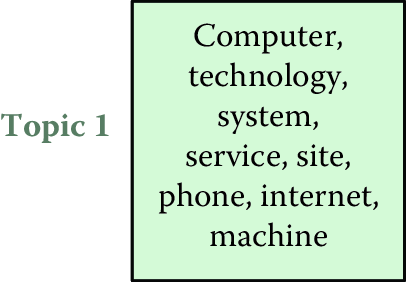
\includegraphics[width=0.7\linewidth]{ChapterText/figures/nyt_topics-1} \end{center}

\begin{center}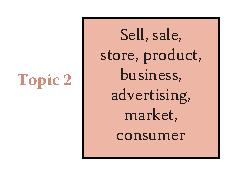
\includegraphics[width=0.7\linewidth]{ChapterText/figures/nyt_topics-2} \end{center}\begin{figure}

{\centering 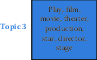
\includegraphics[width=0.7\linewidth]{ChapterText/figures/nyt_topics-3} 

}

\caption{Topics are distributions over words. Here are three example topics learned by latent Dirichlet allocation from a model with 50 topics discovered from the *New York Times* [@sandhaus-08]. Topic 1 seems to be about technology, Topic 2 about business, and Topic 3 about the arts}\label{fig:nyt-topics-3}
\end{figure}

In addition to assuming that there exist some number of topics that
explain a corpus, LDA also assumes that each document in a corpus can be
explained by a small number of topics. For example, taking the example
topics from Figure \ref{fig:nyt-topics-3}, a document titled ``Red
Light, Green Light: A Two-Tone LED to Simplify Screens'' would be about
Topic 1, which appears to be about technology. However, a document like
``Forget the Bootleg, Just Download the Movie Legally'' would require
all three of the topics. The set of topics that are used by a document
is called the document's \emph{allocation} (Figure
\ref{fig:nyt-documents}). This terminology explains the name
\emph{latent Dirichlet allocation}: each document has an allocation over
latent topics governed by a Dirichlet distribution.

\begin{figure}

{\centering 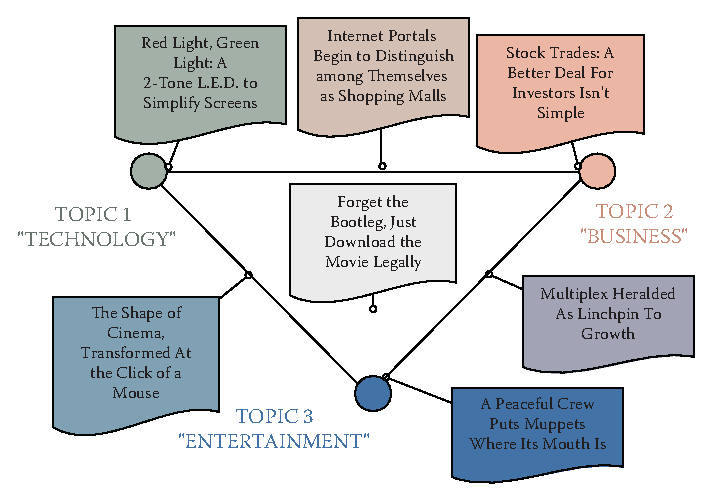
\includegraphics[width=0.7\linewidth]{ChapterText/figures/nyt_documents} 

}

\caption{Allocations of documents to topics}\label{fig:nyt-documents}
\end{figure}

\vspace*{-12pt}

\subsubsection{\texorpdfstring{Inferring ``topics'' from raw
text}{Inferring topics from raw text}}\label{inferring-topics-from-raw-text}

Algorithmically, the problem can be viewed as a black box. Given a
corpus and an integer \(K\) as input, provide the topics that best
describe the document collection: a process called \emph{posterior
inference}. The most common algorithm for solving this problem is a
technique called \emph{Gibbs sampling} (Geman and Geman
\protect\hyperlink{ref-geman-90}{1990}).

Gibbs sampling works at the word level to discover the topics that best
describe a document collection. Each word is associated with a single
topic, explaining why that word appeared in a document. For example,
consider the sentence ``Hollywood studios are preparing to let people
download and buy electronic copies of movies over the Internet.'' Each
word in this sentence is associated with a topic: ``Hollywood'' might be
associated with an arts topic; ``buy'' with a business topic; and
``Internet'' with a technology topic (Figure \ref{fig:inference-1}).

\enlargethispage{18pt}

\begin{figure}

{\centering 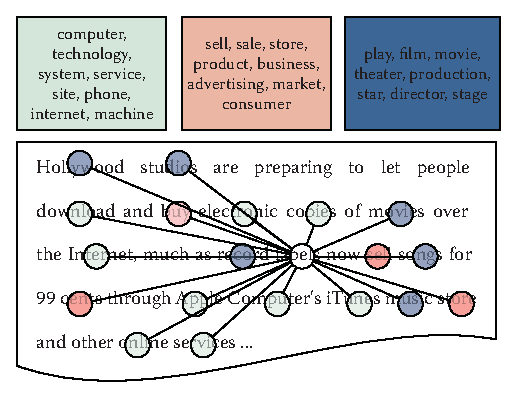
\includegraphics[width=0.7\linewidth]{ChapterText/figures/inference_1} 

}

\caption{Each word is associated with a topic. Gibbs sampling inference iteratively resamples the topic assignments for each word to discover the most likely topic assignments that explain the document collection}\label{fig:inference-1}
\end{figure}

This is where we should eventually get. However, we do not know this to
start. So we can initially assign words to topics randomly. This will
result in poor topics, but we can make those topics better. We improve
these topics by taking each word, pretending that we do not know the
topic, and selecting a new topic for the word.

A topic model wants to do two things: it does not want to use many
topics in a document, and it does not want to use many words in a topic.
So the algorithm will keep track of how many times a document \(d\) has
used a topic \(k\), \(N_{d,k}\), and how many times a topic \(k\) has
used a word \(w\), \(V_{k,w}\). For notational convenience, it will also
be useful to keep track of marginal counts of how many words are in a
document, \[N_{d, \cdot} \equiv \sum_k N_{d,k},\] and how many words are
associated with a topic, \[V_{k, \cdot} \equiv \sum_w V_{k, w}.\] The
algorithm removes the counts for a word from \(N_{d,k}\) and \(V_{k,w}\)
and then changes the topic of a word (hopefully to a better topic than
the one it had before). Through many thousands of iterations of this
process, the algorithm can find topics that are coherent, useful, and
characterize the data well.

The two goals of topic modeling---balancing document allocations to
topics and topics' distribution over words---come together in an
equation that multiplies them together. A good topic will be both common
in a document and explain a word's appearance well.

\begin{center}\rule{0.5\linewidth}{\linethickness}\end{center}

\textbf{Example: Gibbs sampling for topic models}

The topic assignment \(z_{d,n}\) of word \(n\) in document \(d\) is
proportional to
\[p(z_{d,n}=k) \propto \left( \underset{how much doc likes the topic}{\frac{N_{d,k} + \alpha}{N_{d, \cdot} + K \alpha}} \right) \left(\underset{how much topic likes the word}{\frac{V_{k,w_{d,n}} + \beta}{V_{k, \cdot} + V \beta}} \right),\]
where \(\alpha\) and \(\beta\) are smoothing factors that prevent a
topic from having zero probability if a topic does not use a word or a
document does not use a topic (Wallach, Mimno, and McCallum
\protect\hyperlink{ref-wallach-09b}{2009}). Recall that we do not
include the token that we are sampling in the counts for \(N\) or \(V\).

For the sake of concreteness, assume that we have three documents with
the following topic assignments:

\begin{itemize}
\item
  Document 1: \(^A\)dog\(_3\) \(^B\)cat\(_2\) \(^C\)cat\(_3\)
  \(^D\)pig\(_1\)
\item
  Document 2: \(^E\)hamburger\(_2\) \(^F\)dog\(_3\)
  \(^G\)hamburger\(_1\)
\item
  Document 3: \(^H\)iron\(_1\) \(^I\)iron\(_3\) \(^J\)pig\(_2\)
  \(^K\)iron\(_2\)
\end{itemize}

If we want to sample token B (the first instance of of ``cat'' in
document 1), we compute the conditional probability for each of the
three topics (\(z=1,2,3\)): \[\begin{aligned}
p(z_B = 1) = & \frac{1 + 1.000}{3 + 3.000} \times \frac{0
    + 1.000}{3 + 5.000} = 0.333 \times 0.125 = 0.042, \\[4pt]
p(z_B = 2) = & \frac{0 + 1.000}{3 + 3.000} \times \frac{0
    + 1.000}{3 + 5.000} = 0.167 \times 0.125 = 0.021\mbox{, and} \\[4pt]
p(z_B = 3) = & \frac{2 + 1.000}{3 + 3.000} \times \frac{1 + 1.000}{4 + 5.000} = 0.500 \times 0.222 = 0.111.\end{aligned}\]
To reiterate, we do not include token B in these counts: in computing
these conditional probabilities, we consider topic 2 as never appearing
in the document and ``cat'' as never appearing in topic 2. However,
``cat'' does appear in topic 3 (token C), so it has a higher probability
than the other topics. After renormalizing, our conditional
probabilities are \((0.24, 0.12, 0.64)\). We then sample the new
assignment of token B to be topic 3 two times out of three. Griffiths
and Steyvers (Griffiths and Steyvers
\protect\hyperlink{ref-griffiths-04}{2004}) provide more details on the
derivation of this equation.

\textbf{Example code}

\subsubsection{Applications of topic
models}\label{applications-of-topic-models}

Topic modeling is most often used for topic exploration, allowing users
to understand the contents of large text corpora. Thus, topic models
have been used, for example, to understand what the National Institutes
of Health funds (Talley et al.
\protect\hyperlink{ref-talley2011database}{2011}); to compare and
contrast what was discussed in the North and South in the Civil War
(Nelson \protect\hyperlink{ref-nelson-10}{2010}); and to understand how
individuals code in large programming projects (Maskeri, Sarkar, and
Heafield \protect\hyperlink{ref-maskeri-08}{2008}).

Topic models can also be used as features to more elaborate algorithms
such as machine translation (Hu et al.
\protect\hyperlink{ref-Hu:Zhai:Eidelman:Boyd-Graber-2014}{2014}),
detecting objects in images (Wang, Blei, and Fei-Fei
\protect\hyperlink{ref-wang-09b}{2009}), or identifying political
polarization (Paul and Girju \protect\hyperlink{ref-paul-10}{2010}).
Find a good example of topic models used in social sciences (maybe
political science)

Evaluating clustering methods for text analysis

Objective evaluation Task specific evaluation

\textbf{Document classification}

The section above focused on the task of finding topics and themes in a
new text data set. In many cases, we already know a set of topics - this
could be the set of topics or research fields as described by the Social
Science Research Network or the set of sections (local news,
international, sports, finance, etc.) in a news publication. The task we
often face is to automatically categorize new documents into an existing
set of categories. In text analysis, this is called text classification
or categorization and uses supervised learning techniques from machine
learning described in the earlier chapter.

Text classification typically requires two things: A set of categories
we want documents to be categorized into (each document can belong to
one or more categories) Set of documents annotated/tagged with one or
more categories from step 1.

For example, if we want to classify twitter or facebook posts as being
about health or finance, a classification method would take a small
number of posts, manually tagged as belonging to either health or
finance, and train a classification model. This model can then be used
to automatically classify new posts as belonging to either health or
finance

\textbf{Diagram of Text Classification Pipeline}

Processing -\textgreater{} linguistic - \textgreater{} matrix
-\textgreater{} classification method

All of the classification (supervised learning) methods we covered in
the Machine Learning chapter can be used here once the text data has
been processed and converted to a matrix. Neural Networks
{[}reference{]},. Random Forests {[}ref{]}, and Support Vector Machines
{[}ref{]} are some of the commonly used methods applied to text data.

\begin{center}\rule{0.5\linewidth}{\linethickness}\end{center}

\textbf{Example: Using text to categorize scientific fields}

The National Center for Science and Engineering Statistics, the US
statistical agency charged with collecting statistics on science and
engineering, uses a rule-based system to manually create categories of
science; these are then used to categorize research as ``physics'' or
``economics'' (Mortensen, Bloch, and others
\protect\hyperlink{ref-oecd2005measurement}{2005}; Economic Co-operation
and Development \protect\hyperlink{ref-manual2004summary}{2004}). In a
rule-based system there is no ready response to the question ``how much
do we spend on climate change, food safety, or biofuels?'' because
existing rules have not created such categories. Text analysis
techniques can be used to provide such detail without manual collation.
For example, data about research awards from public sources and about
people funded on research grants from UMETRICS can be linked with data
about their subsequent publications and related student dissertations
from ProQuest. Both award and dissertation data are text documents that
can be used to characterize what research has been done, provide
information about which projects are similar within or across
institutions, and potentially identify new fields of study (Talley et
al. \protect\hyperlink{ref-talley2011database}{2011}).

\textbf{Evaluating Text Classification Methods}

The metrics used to evaluate text classification methods are the same as
those used in supervised learning, as described in the Machine Learning
chapter. The most commonly used metrics include accuracy, precision,
recall, AUC, and F1 score. {[}include example in notebook{]}

\textbf{Applications} \vspace*{-2pt}

\textbf{Spam Detection}

One simple but ubiquitous example of document classification is spam
detection: an email is either an unwanted advertisement (spam) or it is
not. Document classification techniques such as naïve Bayes (Lewis
\protect\hyperlink{ref-lewis-05}{1998}) touch essentially every email
sent worldwide, making email usable even though most emails are spam.

\textbf{Sentiment analysis}

Instead of being what a document is about, a label \(y\) could also
reveal the speaker. A recent subfield of natural language processing is
to use machine learning to reveal the internal state of speakers based
on what they say about a subject (Pang and Lee
\protect\hyperlink{ref-pang-08}{2008}). For example, given an example of
sentence \(x\), can we determine whether the speaker is a Liberal or a
Conservative? Is the speaker happy or sad?

Simple approaches use dictionaries and word counting methods (Pennebaker
and Francis \protect\hyperlink{ref-pennebaker-99}{1999}), but more
nuanced approaches make use of \emph{domain}-specific information to
make better predictions. One uses different approaches to praise a
toaster than to praise an air conditioner (Blitzer, Dredze, and Pereira
\protect\hyperlink{ref-blitzer-07}{2007}); liberals and conservatives
each frame health care differently from how they frame energy policy
(Nguyen, Boyd-Graber, and Resnik
\protect\hyperlink{ref-nguyen-13:shlda}{2013}).

\section{Word Embeddings and Deep
Learning}\label{word-embeddings-and-deep-learning}

\section{Text analysis tools}\label{text-analysis-tools}

We are fortunate to have access to a set of powerful open source text
analysis tools. We describe three here.

\textbf{The Natural Language Toolkit}

The NLTK is a commonly used natural language toolkit that provides a
large number of relevant solutions for text analysis. It is Python-based
and can be easily integrated into data processing and analytical scripts
by a simple \texttt{import\ nltk} (or similar for any one of its
submodules).

The NLTK includes a set of tokenizers, stemmers, lemmatizers and other
natural language processing tools typically applied in text analysis and
machine learning. For example, a user can extract tokens from a document
\emph{doc} by running the command
\texttt{tokens\ =\ nltk.word\_tokenize(doc)}.

Useful text corpora are also present in the NLTK distribution. For
example, the stop words list can be retrieved by running the command
\texttt{stops=nltk.corpus.stopwords.words(language)}. These stop words
are available for several languages within NTLK, including English,
French, and Spanish.

Similarly, the Brown Corpus or WordNet can be called by running
\texttt{from\ nltk.corpus\ import\ wordnet/brown}. After the corpora are
loaded, their various properties can be explored and used in text
analysis; for example,
\texttt{dogsyn\ =\ wordnet.synsets(\textquotesingle{}dog\textquotesingle{})}
will return a list of WordNet synsets related to the word ``dog.''

Term frequency distribution and \(n\)-gram indexing are other techniques
implemented in NLTK. For example, a user can compute frequency
distribution of individual terms within a document \emph{doc} by running
a command in Python: \texttt{fdist=nltk.FreqDist(text)}. This command
returns a dictionary of all tokens with associated frequency within
\emph{doc}.

\(N\)-gram indexing is implemented as a chain-linked collocations
algorithm that takes into account the probability of any given two,
three, or more words appearing together in the entire corpus. In
general, \(n\)-grams can be discovered as easily as running
\texttt{bigrams\ =\ nltk.bigrams(text)}. However, a more sophisticated
approach is needed to discover statistically significant word
collocations, as we show in Listing 7.4.

Bird et al. (Bird, Klein, and Loper
\protect\hyperlink{ref-bird-09}{2009}) provide a detailed description of
NLTK tools and techniques. See also the official NLTK website (NLTK
Project, n.d.).

\begin{Shaded}
\begin{Highlighting}[]
\NormalTok{def }\KeywordTok{bigram_finder}\NormalTok{(texts)}\OperatorTok{:}
\StringTok{  }\CommentTok{# NLTK bigrams from a corpus of documents separated by new line}
\StringTok{  }\NormalTok{tokens_list =}\StringTok{ }\KeywordTok{nltk.word_tokenize}\NormalTok{(}\KeywordTok{re.sub}\NormalTok{(}\StringTok{"}\CharTok{\textbackslash{}n}\StringTok{"}\NormalTok{,}\StringTok{" "}\NormalTok{,texts))}
\NormalTok{  bgm    =}\StringTok{ }\KeywordTok{nltk.collocations.BigramAssocMeasures}\NormalTok{()}
\NormalTok{  finder =}\StringTok{ }\KeywordTok{nltk.collocations.BigramCollocationFinder.from_words}\NormalTok{(tokens_list)}
\NormalTok{  scored =}\StringTok{ }\KeywordTok{finder.score_ngrams}\NormalTok{( bgm.likelihood_ratio  )}

  \CommentTok{# Group bigrams by first word in bigram.}
\NormalTok{  prefix_keys =}\StringTok{ }\KeywordTok{collections.defaultdict}\NormalTok{(list)}
  \ControlFlowTok{for}\NormalTok{ key, scores }\ControlFlowTok{in}\NormalTok{ scored}\OperatorTok{:}
\StringTok{      }\NormalTok{prefix_keys[key[}\DecValTok{0}\NormalTok{]]}\KeywordTok{.append}\NormalTok{((key[}\DecValTok{1}\NormalTok{], scores))}

  \CommentTok{# Sort keyed bigrams by strongest association.}
  \ControlFlowTok{for}\NormalTok{ key }\ControlFlowTok{in}\NormalTok{ prefix_keys}\OperatorTok{:}
\StringTok{      }\NormalTok{prefix_keys[key]}\KeywordTok{.sort}\NormalTok{(}\DataTypeTok{key =}\NormalTok{ lambda x}\OperatorTok{:}\StringTok{ }\OperatorTok{-}\NormalTok{x[}\DecValTok{1}\NormalTok{])}
\end{Highlighting}
\end{Shaded}

Listing 7.4. Python code to find bigrams using NLTK

\textbf{Stanford CoreNLP}

While NLTK's emphasis is on simple reference implementations, Stanford's
CoreNLP (Stanford, n.d.; Manning et al.
\protect\hyperlink{ref-manning2014stanford}{2014}) is focused on fast
implementations of cutting-edge algorithms, particularly for syntactic
analysis (e.g., determining the subject of a sentence).

\textbf{MALLET}

For probabilistic models of text, MALLET, the MAchine Learning for
LanguagE Toolkit (McCallum \protect\hyperlink{ref-mallet}{2002}), often
strikes the right balance between usefulness and usability. It is
written to be fast and efficient but with enough documentation and easy
enough interfaces to be used by novices. It offers fast, popular
implementations of conditional random fields (for part-of- speech
tagging), text classification, and topic modeling.

\section{Summary}\label{summary-4}

Many of the new sources of data that are of interest to social
scientists is text: tweets, Facebook posts, corporate emails, and the
news of the day. However, the meaning of these documents is buried
beneath the ambiguities and noisiness of the informal, inconsistent ways
by which humans communicate with each other and traditional data
analysis methods do not work with text data directly. Despite attempts
to formalize the meaning of text data through asking users to tag
people, apply metadata, or to create structured representations, these
attempts to manually curate meaning are often incomplete, inconsistent,
or both.

These aspects make text data difficult to work with, but also a
rewarding object of study. Unlocking the meaning of a piece of text
helps bring machines closer to human-level intelligence---as language is
one of the most quintessentially human activities---and helps overloaded
information professionals do their jobs more effectively: understand
large corpora, find the right documents, or automate repetitive tasks.
And as an added bonus, the better computers become at understanding
natural language, the easier it is for information professionals to
communicate their needs: one day using computers to grapple with big
data may be as natural as sitting down for a conversation over coffee
with a knowledgeable, trusted friend.

\section{Resources}\label{resources-3}

\textbf{Text corpora}

A set of multiple similar documents is called a \emph{corpus}. For
example, the Brown University Standard Corpus of Present-Day American
English, or just the Brown Corpus (Francis and Kucera
\protect\hyperlink{ref-browncorpus}{1979}), is a collection of processed
documents from works published in the United States in 1961. The Brown
Corpus was a historical milestone: it was a machine-readable collection
of a million words across 15 balanced genres with each word tagged with
its part of speech (e.g., noun, verb, preposition). The British National
Corpus (University of Oxford \protect\hyperlink{ref-bnc}{2006}) repeated
the same process for British English at a larger scale. The Penn
Treebank (Marcus, Santorini, and Marcinkiewicz
\protect\hyperlink{ref-marcus-93}{1993}) provides additional
information: in addition to part-of-speech annotation, it provides
\emph{syntactic} annotation. For example, what is the object of the
sentence ``The man bought the hat''? These standard corpora serve as
training data to train the classifiers and machine learning techniques
to automatically analyze text (Halevy, Norvig, and Pereira
\protect\hyperlink{ref-halevy-09}{2009}).

Text analysis is one of the more complex tasks in big data analysis.
Because it is unstructured, text (and natural language overall) requires
significant processing and cleaning before we can engage in interesting
analysis and learning. In this chapter we have referenced several
resources that can be helpful in mastering text mining techniques:

\begin{itemize}
\item
  The Natural Language Toolkit is one of the most popular Python-based
  tools for natural language processing. It has a variety of methods and
  examples that are easily accessible online (NLTK Project, n.d.). The
  book by Bird et al. (Bird, Klein, and Loper
  \protect\hyperlink{ref-bird-09}{2009}), available online, contains
  multiple examples and tips on how to use NLTK.
\item
  The book \emph{Pattern Recognition and Machine Learning} by
  Christopher Bishop (Bishop \protect\hyperlink{ref-bishop-06}{2006}) is
  a useful introduction to computational techniques, including
  probabilistic methods, text analysis, and machine learning. It has a
  number of tips and examples that are helpful to both learning and
  experienced researchers.
\item
  A paper by Anna Huang (Huang \protect\hyperlink{ref-huang-08}{2008})
  provides a brief overview of the key similarity measures for text
  document clustering discussed in this chapter, including their
  strengths and weaknesses in different contexts.
\item
  Materials at the MALLET website (McCallum
  \protect\hyperlink{ref-mallet}{2002}) can be specialized for the
  unprepared reader but are helpful when looking for specific solutions
  with topic modeling and machine classification using this toolkit.
\item
  David Blei, one of the authors of the latent Dirichlet allocation
  algorithm (topic modeling), maintains a helpful web page with
  introductory resources for those interested in topic modeling (Blei,
  n.d.).
\item
  We provide an example of how to run topic modeling using MALLET on
  textual data from the National Science Foundation and Norwegian
  Research Council award abstracts (Boyd-Graber, n.d.).
\end{itemize}

\hypertarget{chap:networks}{\chapter{Networks: The
Basics}\label{chap:networks}}

\textbf{Jason Owen-Smith}

Social scientists are typically interested in describing the activities
of individuals and organizations (such as households and firms) in a
variety of economic and social contexts. The frame within which data has
been collected will typically have been generated from tax or other
programmatic sources. The new types of data permit new units of
analysis---particularly network analysis---largely enabled by advances
in mathematical graph theory. This chapter provides an overview of how
social scientists can use network theory to generate measurable
representations of patterns of relationships connecting entities. The
value of the new framework is not only in constructing different
right-hand-side variables but also in studying an entirely new unit of
analysis that lies somewhere between the largely atomistic actors that
occupy the markets of neo-classical theory and the tightly managed
hierarchies that are the traditional object of inquiry of sociologists
and organizational theorists.

\textbf{Structure:}

\begin{itemize}
\tightlist
\item
  What is network analysis useful for? - motivating examples and use
  cases
\item
  What is network analysis
\item
  What are graphs - types of graphs, vocabulary
\item
  Representation, etc.
\item
  How to create networks?
\item
  How to analyze networks?
\item
  network measures - definitions
\item
  Network visualization
\item
  Answering questions through network analysis
\item
  More examples
\item
  Tools
\item
  Summary
\end{itemize}

\section{Introduction}\label{introduction-3}

Social Scientists have studies networks for a long time. A lot of the
theory behind network analysis in fact comes from the social sciences
where we studied relationships between people, groups, and organizations
{[}citation Moreno, J.L., Jennings, H.H.: Who Shall Survive?: A New
Approach to the Problem of Human Interrelations. Nervous and Mental
Disease Publishing Co., Washington, D.C. (1934). What's different today
is the scale of the data available to us to perform this analysis.
Instead of studying a group of 25 participants in a karate club
(citation), we now have data about 100s of millions of people
communicating with each other online through social media channels, or
hundreds of thousands of employees in a large multinational
organizations collaborating on projects. This increased scale requires
us to explore new methods of answering the same questions that we used
to be interested in, as well as opens up avenues to answer new questions
that could not be answered before.

\begin{center}\rule{0.5\linewidth}{\linethickness}\end{center}

\textbf{\emph{Box with examples or references to these examples}}

Survey paper: (maybe at end in further reading)
\url{http://keg.cs.tsinghua.edu.cn/jietang/publications/WWW17-Tang-Comp-Social-Science-Survey.pdf}

\url{http://www.sn.ethz.ch//} Zurich Networks Labs

Example 1:
\url{https://cs.stanford.edu/people/jure/pubs/recurrence-www16.pdf}

Example 2: \url{https://abjer.github.io/project/social-fabric/} or
\url{https://www.ncbi.nlm.nih.gov/pmc/articles/PMC4000208/} (same study)

Example 3: diffusion of information

Facebook graph example:
\url{http://snap.stanford.edu/class/cs224w-readings/backstrom12fb.pdf}

\begin{center}\rule{0.5\linewidth}{\linethickness}\end{center}

This chapter provides a basic introduction to the analysis of large
networks. We describe how to use data from existing social networks as
well as how to turn ``non-network'' data into a network to perform
further analysis. We then describe different measures that can be
calculated to understand the properties of the network being analyzed,
show different network visualization technique, and discuss social
science questions that these network measures and visualizations can
help us answer.

We use the comparison of the collaboration networks of two
research-intensive universities to show how to perform network analysis
but the same approach generalizes to other types of problems. The
collaboration networks and a grant co-employment network for a large
public university examined in this chapter are derived from data
produced by the multi-university Committee on Institutional Cooperation
(CIC)'s UMETRICS project (Lane et al.
\protect\hyperlink{ref-lane2015new}{2015}). The snippets of code that
are provided are from the \texttt{igraph} package for network analysis
as implemented in Python.

What are networks?

Networks are measurable representations of relationships connecting
entities. What this means is that there are two fundamental questions to
ask of any network representation: First, what are the nodes? Second,
what are the relationships (ties) connecting the nodes? Once we have the
representation set up, we can then analyze the underlying data and
relationships through the measures and methods described in this
chapter. This is of great interest because a great deal of research in
social sciences demonstrates that networks are essential to
understanding behaviors and outcomes at both the individual and the
organizational level.

Networks offer not just another convenient set of right-hand-side
variables, but an entirely new unit of analysis that lies somewhere
between the largely atomistic actors that occupy the markets of
neo-classical theory and the tightly managed hierarchies that are the
traditional object of inquiry of sociologists and organizational
theorists. As Walter W. Powell (Powell
\protect\hyperlink{ref-powell2003neither}{2003}) puts it in a
description of buyer supplier networks of small Italian firms: ``when
the entangling of obligation and reputation reaches a point where the
actions of the parties are interdependent, but there is no common
ownership or legal framework \ldots{} such a transaction is neither a
market exchange nor a hierarchical governance structure, but a separate,
different mode of exchange.''

Existing as they do between the uncoordinated actions of independent
individuals and coordinated work of organizations, networks offer a
unique level of analysis for the study of scientific and creative teams
(Wuchty, Jones, and Uzzi
\protect\hyperlink{ref-wuchty2007increasing}{2007}), collaborations
(Kabo et al. \protect\hyperlink{ref-kabo2015shared}{2015}), and clusters
of entrepreneurial firms (Owen-Smith and Powell
\protect\hyperlink{ref-owen2004knowledge}{2004}).

The following sections will introduce you to this approach to studying
innovation and discovery, focusing on examples drawn from
high-technology industries and particularly from the scientific
collaborations among grant-employed researchers at UMETRICS
universities. I make particular use of a network that connects
individual researchers to grants that paid their salaries in 2012 for a
large public university. The grants network for university A includes
information on 9,206 individuals who were employed on 3,389 research
grants from federal science agencies in a single year. The web of
partnerships that emerges from university scientists' decentralized
efforts to build effective collaborations and teams generates a
distinctive social infrastructure for cutting- edge Science.

While this chapter focuses my attention on social networks, you could
easily use the techniques described here to examine the structure of
networks such as the World Wide Web, the national railway route map of
the USA, the food web of an ecosystem, or the neuronal network of a
particular species of animal.

The chapter first introduces the most common structures for large
network data, briefly introduce three key social ``mechanisms of
action'' by which social networks are thought to have their effects, and
then present a series of basic measures that can be used to quantify
characteristics of entire networks and the relative position individual
people or organizations hold in the differentiated social structure
created by networks.

Taken together, these measures offer an excellent starting point for
examining how global network structures create opportunities and
challenges for the people in them, for comparing and explaining the
productivity of collaborations and teams, and for making sense of the
differences between organizations, industries, and markets that hinge on
the pattern of relationships connecting their participants.

\enlargethispage{12pt} Understanding the productivity and effects of
university research thus requires an effort to measure and characterize
the networks on which it depends. As suggested, those networks influence
outcomes in three ways: first, they distinguish among individuals;
second, they differentiate among teams; and third, they help to
distinguish among research-performing universities. Most
research-intensive institutions have departments and programs that cover
similar arrays of topics and areas of study. What distinguishes them
from one another is not the topics they cover but the ways in which
their distinctive collaboration networks lead them to have quite
different scientific capabilities.

\section{Turning Data into a Network}\label{turning-data-into-a-network}

Networks are comprised of \emph{nodes}, which represent things that can
be connected to one another, and of ties that represent the
relationships connecting nodes. When ties are undirected they are called
\emph{edges}. When they are directed (as when I lend money to you and
you do or do not reciprocate) they are called \emph{arcs}. Nodes, edges
and arcs can, in principle, be anything: patents and citations, web
pages and hypertext links, scientists and collaborations, teenagers and
intimate relationships, nations and international trade agreements. The
very flexibility of network approaches means that the first step toward
doing a network analysis is to first turn our data into a graph by
clearly defining what counts as a node and what counts as a tie. In
traditional social network analysis studies, there is a natural
representation of the data as a network. People are often nodes, and
some type of communication between them form the ``ties''. While this
seems like an easy move, it often requires deep thought. For instance,
an interest in innovation and discovery could take several forms. We
could be interested in how universities differ in their capacity to
respond to new requests for proposals (a macro question that would
require the comparison of full networks across campuses). We could
wonder what sorts of training arrangements lead to the best outcomes for
graduate students (a more micro- level question that requires us to
identify individual positions in larger networks). Or we could ask what
team structure is likely to lead to more or less radical discoveries (a
decidedly meso-level question that requires we identify substructures
and measure their features).

Each of these is a network question that relies on the ways in which
people are connected to one another. The first challenge of measurement
is to identify the nodes (what is being connected) and the ties (the
relationships that matter) in order to construct the relevant networks.
The next is to collect and structure the data in a fashion that is
sufficient for analysis. Finally, measurement and visualization
decisions must be made.

\subsection{Types of Networks}\label{types-of-networks}

\begin{center}\rule{0.5\linewidth}{\linethickness}\end{center}

\textbf{Vocabulary box: network terminology{]} - }Nodes\textbf{: -
}Ties\textbf{: - }Edges\textbf{: - }Directed\textbf{: - }Undirected**:

\begin{center}\rule{0.5\linewidth}{\linethickness}\end{center}

Network ties can be directed (flowing from one node to another) or
undirected. In either case they can be binary (indicating the presence
or absence of a tie) or valued (allowing for relationships of different
types or strengths). Network data can be represented in matrices or as
lists of edges and arcs. All these types of relationships can connect
one type of node (what is commonly called \emph{one-mode} network data)
or multiple types of nodes (what is called \emph{two-mode} or
affiliation data). Varied data structures correspond to different
classes of network data. The simplest form of network data represents
instances where the same kinds of nodes are connected by undirected ties
(edges) that are binary. An example of this type of data is a network
where nodes are firms and ties indicate the presence of a strategic
alliance connecting them (Powell et al.
\protect\hyperlink{ref-powell2005network}{2005}). This network would be
represented as a square symmetric matrix or a list of edges connecting
nodes. Figure \ref{fig:fig8-1} summarizes this simple data structure,
highlighting the idea that network data of this form can be represented
either as a matrix or as an edge list. If this data was representing
acquisitions, we could turn it into a directed graph where the edge
would be directed from the acquiring firm to the acquired firm.

\begin{figure}

{\centering 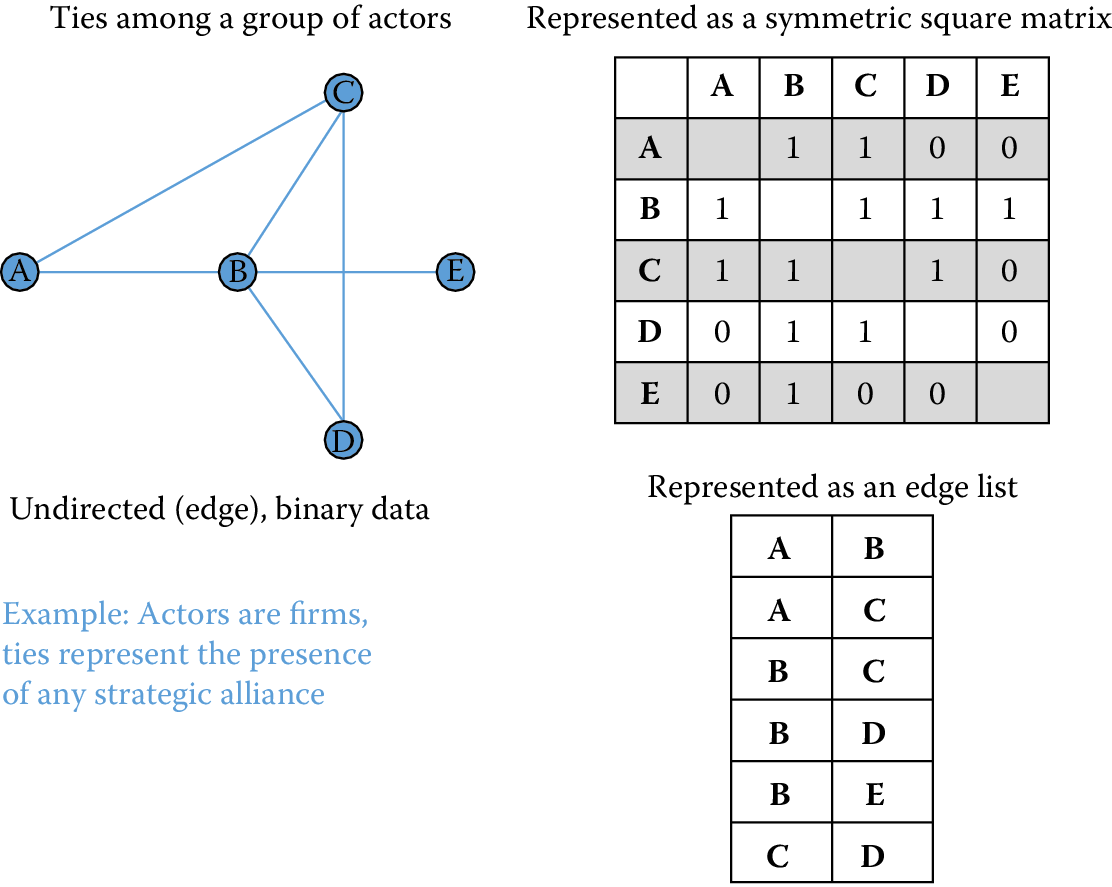
\includegraphics[width=0.7\linewidth]{ChapterNetworks/figures/fig8-1} 

}

\caption{Undirected, binary, one-mode network data}\label{fig:fig8-1}
\end{figure}

\vspace*{-12pt} A much more complicated network would be one that is
both directed and valued. One example might be a network of nations
connected by flows of international trade. Goods and services flow from
one nation to another and the value of those goods and services (or
their volume) represents ties of different strengths. When networks
connecting one class of nodes (in this case nations) are directed and
valued, they can be represented as asymmetric valued matrices or lists
of arcs with associated values. (See Figure \ref{fig:fig8-1}.)

\begin{figure}

{\centering 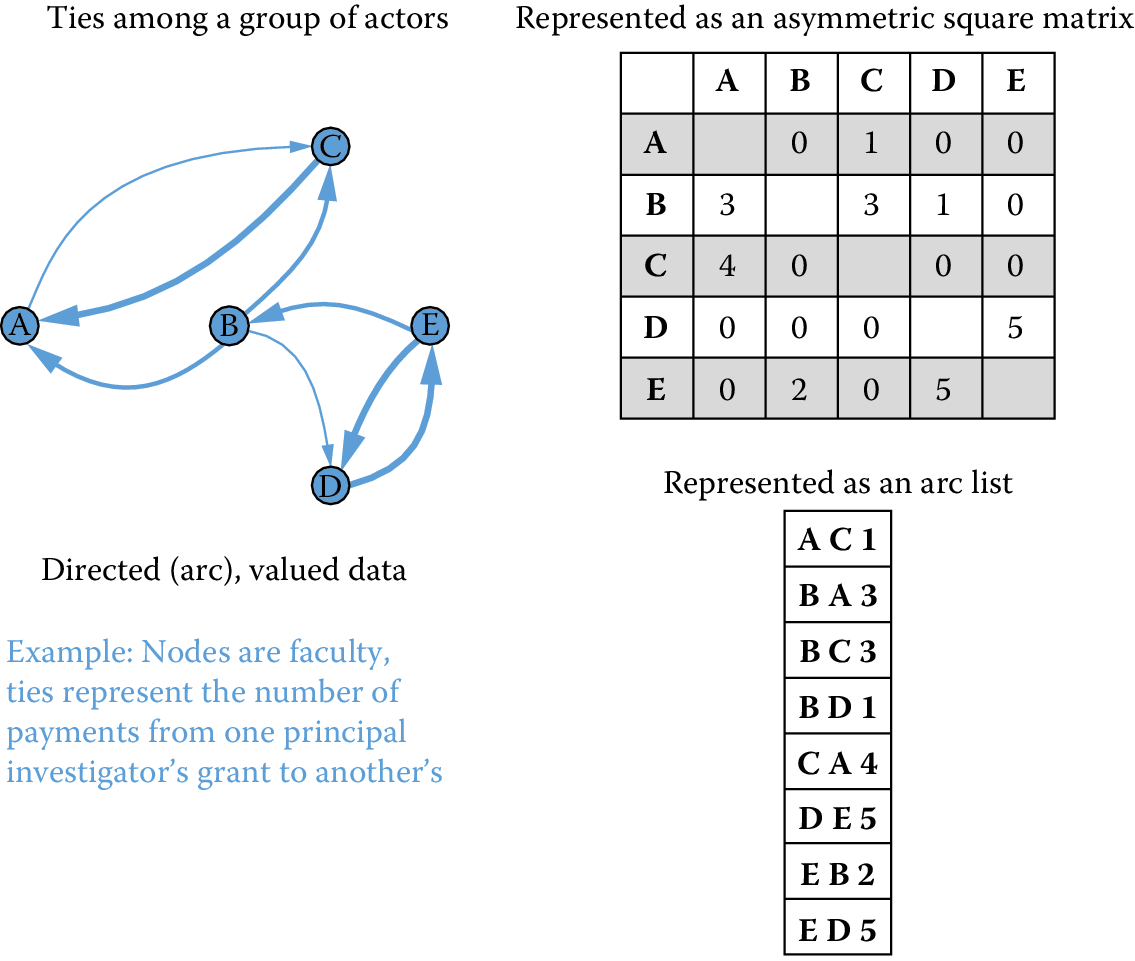
\includegraphics[width=0.7\linewidth]{ChapterNetworks/figures/fig8-2} 

}

\caption{Directed, valued, one-mode network data}\label{fig:fig8-2}
\end{figure}

\vspace*{-12pt} While many studies of small- to medium-sized social
networks rely on one-mode data. Large-scale social network data of this
type are relatively rare, but one-mode data of this sort are fairly
common in relationships among other types of nodes such as web pages or
citations connecting patents or publications. Nevertheless, much ``big''
social network analysis is conducted using two-mode data. The UMETRICS
employee data set is a two-mode network that connects people (research
employees) to the grants that pay their wages. These two types of nodes
can be represented as a rectangular matrix that is either valued or
binary. It is relatively rare to analyze untransformed two-mode network
data. Instead, most analyses take advantage of the fact that such
networks are \emph{dual} (White, Boorman, and Breiger
\protect\hyperlink{ref-white1976social}{1976}). In other words, a
two-mode network connecting grants and people can be conceptualized (and
analyzed) as two one-mode networks, or \emph{projections}\footnote{Key
  insight: A two-mode network can be conceptualized and analyzed as two
  one-mode networks, or projections.}.

\subsection{Inducing one-mode networks from two-mode
data}\label{inducing-one-mode-networks-from-two-mode-data}

The most important trick in large-scale social network analysis is that
of inducing one-mode, or unipartite, networks (e.g., employee \(\times\)
employee relationships) from two-mode, or bipartite, data. But the
ubiquity and potential value of two-mode data can come at a cost. Not
all affiliations are equally likely to represent real, meaningful
relationships. While it seems plausible to assume that two individuals
paid by the same grant have interactions that reasonably pertain to the
work funded by the grant, this need not be the case.

For example, consider the two-mode grant \(\times\) person network for
university A. I used SQL to create a representation of this network that
is readable by a freeware network visualization program called Pajek
(Batagelj and Mrvar \protect\hyperlink{ref-batagelj1998pajek}{1998}). In
this format, a network is represented as two lists: a \emph{vertex list}
that lists the nodes in the graph and an \emph{edge list} that lists the
connections between those nodes. In our grant \(\times\) person network,
we have two types of nodes, people and grants, and one kind of edge,
used to represent wage payments from grants to individuals.

I present a brief snippet of the resulting network file in what follows,
showing first the initial 10 elements of the vertex list and then the
initial 10 elements of the edge list, presented in two columns for
compactness. (The complete file comprises information on 9,206 employees
and 3,389 grants, for a total of 12,595 vertices and 15,255 edges. The
employees come first in the vertex list, and so the 10 rows shown below
all represent employees.) Each vertex is represented by a vertex
number--label pair and each edge by a pair of vertices plus an optional
value. Thus, the first entry in the edge list (1 10419) specifies that
the vertex with identifier 1 (which happens to be the first element of
the vertex list, which has value ``00100679'') is connected to the
vertex with identifier 10419 by an edge with value 1, indicating that
employee ``00100679'' is paid by the grant described by vertex 10419.

*Grant-Person-Network

\begin{longtable}[]{@{}llll@{}}
\toprule
*Vertices 12595 9206 & & *Edges &\tabularnewline
\midrule
\endhead
1 & ``00100679'' & 1 & 10419\tabularnewline
2 & ``00107462'' & 2 & 10422\tabularnewline
3 & ``00109569'' & 3 & 9855\tabularnewline
4 & ``00145355'' & 3 & 9873\tabularnewline
5 & ``00153190'' & 4 & 9891\tabularnewline
6 & ``00163131'' & 7 & 10432\tabularnewline
7 & ``00170348'' & 7 & 12226\tabularnewline
8 & ``00172339'' & 8 & 10419\tabularnewline
9 & ``00176582'' & 9 & 11574\tabularnewline
10 & ``00203529'' & 10 & 11196\tabularnewline
\bottomrule
\end{longtable}

The network excerpted above is two-mode because it represents
relationships between two different classes of nodes, grants, and
people. In order to use data of this form to address questions about
patterns of collaboration on UMETRICS campuses, we must first transform
it to represent collaborative relationships.

A person-by-person projection of the original two-mode network assumes
that ties exist between people when they are paid by the same grant. By
the same token, a grant-by-grant projection of the original two-mode
network assumes that ties exist between grants when they pay the same
people. Transforming two-mode data into one-mode projections is a fairly
simple matter. If \(\mathbf{X}\) is a rectangular matrix,
\(p \times g\), then a one-mode projection, \(p \times p\), can be
obtained by multiplying \(\mathbf{X}\) by its transpose \(\mathbf{X}'\).
Figure \ref{fig:fig8-3} summarizes this transformation.

\begin{figure}

{\centering 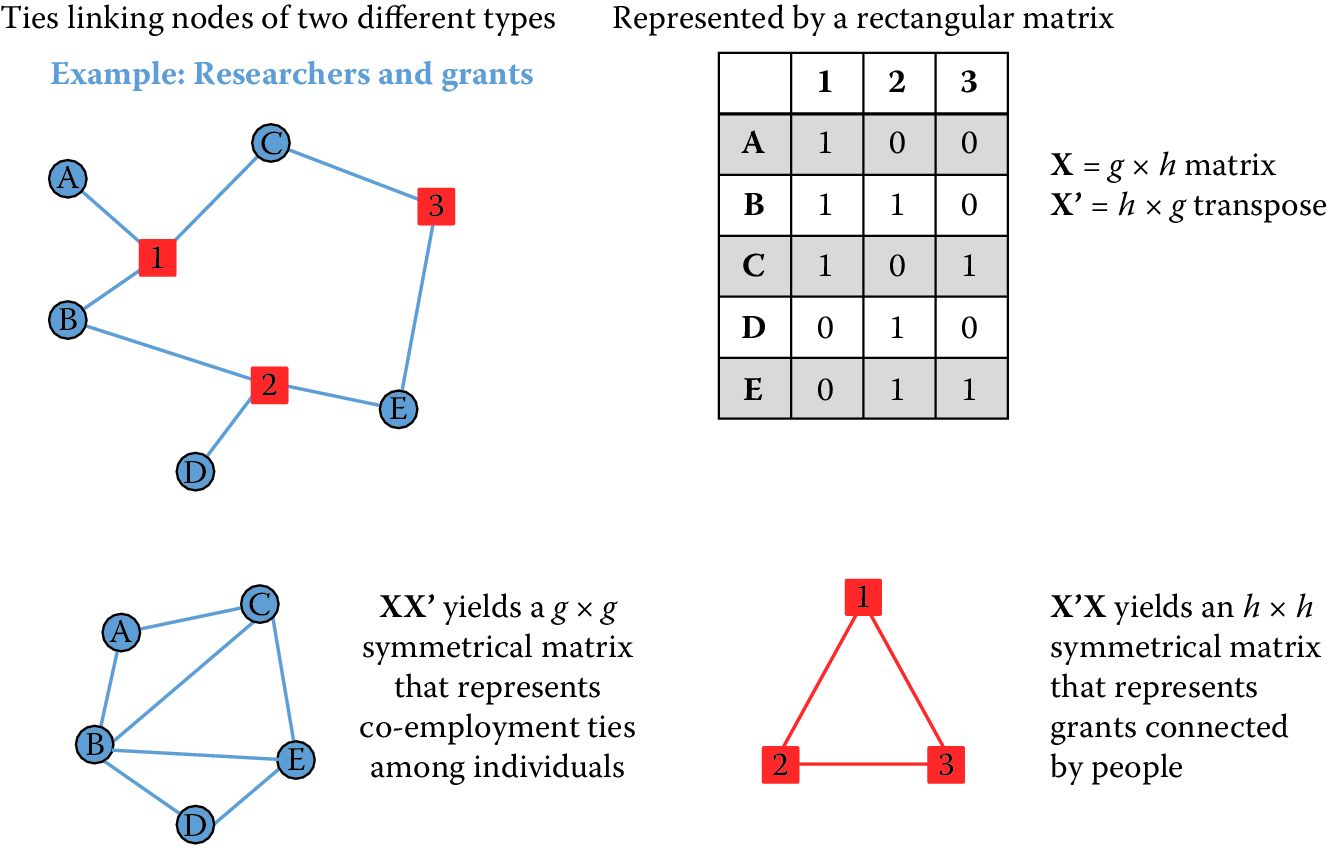
\includegraphics[width=0.7\linewidth]{ChapterNetworks/figures/fig8-3} 

}

\caption{Two-mode affiliation data}\label{fig:fig8-3}
\end{figure}

In the following snippet of code, I use the \texttt{igraph} package in
Python to read in a Pajek file and then transform the original two-mode
network into two separate projections. Because my focus in this
discussion is on relationships among people, I then move on to work
exclusively with the employee-by-employee projection. However, every
technique that I describe below can also be used with the grant-by-grant
projection, which provides a different view of how federally funded
research is put together by collaborative relationships on campus.

\begin{Shaded}
\begin{Highlighting}[]
\NormalTok{from igraph import }\OperatorTok{*}

\CommentTok{# Read the graph}
\NormalTok{g =}\StringTok{ }\KeywordTok{Graph.Read_Pajek}\NormalTok{(}\StringTok{"public_a_2m.net"}\NormalTok{)}

\CommentTok{# Look at result}
\KeywordTok{summary}\NormalTok{(g)}


\CommentTok{# IGRAPH U-WT 12595 15252 --}
\CommentTok{# + attr: color (v), id (v), shape (v), type (v), x (v), y (v), z (v), weight (e)}
\CommentTok{# ...}
\CommentTok{# ...}

\CommentTok{# Transform to get 1M projection}
\NormalTok{pr_g_proj1, pr_g_proj2=}\StringTok{ }\KeywordTok{g.bipartite_projection}\NormalTok{()}

\CommentTok{# Look at results}
\KeywordTok{summary}\NormalTok{(pr_g_proj1)}

\CommentTok{# IGRAPH U-WT 9206 65040 --}
\CommentTok{# + attr: color (v), id (v), shape (v), type (v), x (v), y (v), z (v), weight (e)}

\KeywordTok{summary}\NormalTok{(pr_g_proj2)}
\CommentTok{# IGRAPH U-WT 3389 12510 --}
\CommentTok{# + attr: color (v), id (v), shape (v), type (v), x (v), y (v), z (v), weight (e)}

\CommentTok{# pr_g_proj1 is the employeeXemployee projection, n=9,206 nodes}
\CommentTok{# Rename to emp for use in future calculations}

\NormalTok{emp=pr_g_proj1}
\end{Highlighting}
\end{Shaded}

\vspace*{12pt} We now can work with the graph \texttt{emp}, which
represents the collaborative network of federally funded research on
this campus. Care must be taken when inducing one-mode network
projections from two-mode network data because not all affiliations
provide equally compelling evidence of actual social relationships.
While assuming that people who are paid by the same research grants are
collaborating on the same project seems plausible, it might be less
realistic to assume that all students who take the same university
classes have meaningful relationships. For the remainder of this
chapter, the examples I discuss are based on UMETRICS employee data
rendered as a one-mode person-by-person projection of the original
two-mode person-by-grants data. In constructing these networks I assume
that a tie exists between two university research employees when they
are paid any wages from the same grant during the same year. Other time
frames or thresholds might be used to define ties if appropriate for
particular analyses\footnote{Key insight: Care must be taken when
  inducing one-mode network projections from two-mode network data
  because not all affiliations provide equally compelling evidence of
  actual social relationships.}.

\section{Network measures}\label{network-measures}

The power of networks lies in their unique flexibility and ability to
address many phenomena at multiple levels of analysis. But harnessing
that power requires calculating measures that take into account the
overall structure of relationships represented in a given network. The
key insight of structural analysis is that outcomes for any individual
or group are a function of the complete pattern of connections among
them. In other words, the explanatory power of networks is driven as
much by the pathways that \emph{indirectly} connect nodes as by the
particular relationships that \emph{directly} link members of a given
dyad. Indirect ties create reachability in a network\footnote{Key
  insight: Structural analysis of outcomes for any individual or group
  are a function of the complete pattern of connections among them.}.

\subsection{Reachability}\label{reachability}

Two nodes are said to be reachable when they are connected by an
unbroken chain of relationships through other nodes. For instance, two
people who have never met may nonetheless be able to reach each other
through a common acquaintance who is positioned to broker an
introduction (Obstfeld \protect\hyperlink{ref-obstfeld2005social}{2005})
or the transfer of information and resources (Burt
\protect\hyperlink{ref-burt2004structural}{2004}). It is the
reachability that networks create that makes them so important for
understanding the work of science and innovation.

Consider Figure \ref{fig:fig8-4}, which presents three schematic
networks. In each, one focal node, ego, is colored orange. Each ego has
four alters, but the fact that each has connections to four other nodes
masks important differences in their structural positions. Those
differences have to do with the number of other nodes they can reach
through the network and the extent to which the other nodes in the
network are connected to each other. The orange node (ego) in each
network has four partners, but their positions are far from equivalent.
Centrality measures on full network data can tease out the differences.
The networks also vary in their gross characteristics. Those
differences, too, are measurable\footnote{Key insight: Much of the power
  of networks (and their systemic features) is due to indirect ties that
  create reachability. Two nodes can reach each other if they are
  connected by an unbroken chain of relationships. These are often
  called indirect ties.}.

\begin{figure}

{\centering 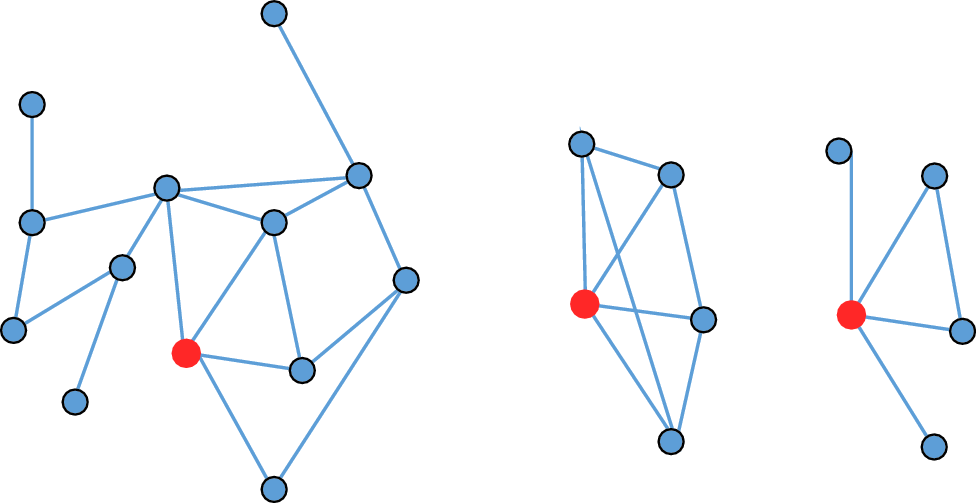
\includegraphics[width=0.7\linewidth]{ChapterNetworks/figures/fig8-4} 

}

\caption{Reachability and indirect ties}\label{fig:fig8-4}
\end{figure}

Networks in which more of the possible connections among nodes are
realized are denser and more cohesive than networks in which fewer
potential connections are realized. Consider the two smaller networks in
Figure \ref{fig:fig8-4}, each of which is comprised of five nodes. Just
five ties connect those nodes in the network on the far right of the
figure. One smaller subset of that network, the triangle connecting ego
and two alters at the center of the image, represents a more cohesively
connected subset of the networks. In contrast, eight of the nine ties
that are possible connect the five nodes in the middle figure; no subset
of those nodes is clearly more interconnected than any other. While
these kinds of differences may seem trivial, they have implications for
the orange nodes, and for the functioning of the networks as a whole.
Structural differences between the positions of nodes, the presence and
characteristics of cohesive ``communities'' within larger networks
(Girvan and Newman \protect\hyperlink{ref-girvan2002community}{2002}),
and many important properties of entire structures can be quantified
using different classes of network measures. Newman (Newman
\protect\hyperlink{ref-newman2010networks}{2010}) provides the most
recent and most comprehensive look at measures and algorithms for
network research.

The most essential thing to be able to understand about larger scale
networks is the pattern of indirect connections among nodes. What is
most important about the structure of networks is not necessarily the
ties that link particular pairs of nodes to one another. Instead, it is
the chains of indirect connections that make networks function as a
system and thus make them worthwhile as new levels of analysis for
understanding social and other dynamics.

\subsection{Whole-network measures}\label{whole-network-measures}

The basic terms needed to characterize whole networks are fairly simple.
It is useful to know the size (in terms of nodes and ties) of each
network you study. This is true both for the purposes of being able to
generally gauge the size and connectivity of an entire network and
because many of the measures that one might calculate using such
networks should be standardized for analytic use. While the list of
possible network measures is long, a few commonly used indices offer
useful insights into the structure and implications of entire network
structures.

\textbf{Components and reachability}

As we have seen, a key feature of networks is reachability. The
reachability of participants in a network is determined by their
membership in what network theorists call \emph{components}, subsets of
larger networks where every member of a group is indirectly connected to
every other. If you imagine a standard node and line drawing of a
network, a component is a portion of the network where you can trace
paths between every pair of nodes without ever having to lift your pen.

Most large networks have a single dominant component that typically
includes anywhere from 50\% to 90\% of its participants as well as many
smaller components and isolated nodes that are disconnected from the
larger portion of the network. Because the path length centrality
measures described below can only be computed on connected subsets of
networks, it is typical to analyze the largest component of any given
network. Thus any description of a network or any effort to compare
networks should report the number of components and the percentage of
nodes reachable through the largest component. In the code snippet
below, I identify the weakly connected components of the employee
network, \texttt{emp}.

\begin{Shaded}
\begin{Highlighting}[]
\CommentTok{# Add component membership}
\NormalTok{emp.vs[}\StringTok{"membership"}\NormalTok{] =}\StringTok{ }\KeywordTok{emp.clusters}\NormalTok{(}\DataTypeTok{mode=}\StringTok{"weak"}\NormalTok{).membership}

\CommentTok{# Add component size}
\NormalTok{emp.vs[}\StringTok{"csize"}\NormalTok{] =}\StringTok{ }\NormalTok{[}\KeywordTok{emp.clusters}\NormalTok{(}\DataTypeTok{mode=}\StringTok{"weak"}\NormalTok{)}\KeywordTok{.sizes}\NormalTok{()[i] }\ControlFlowTok{for}\NormalTok{ i }\ControlFlowTok{in} \KeywordTok{emp.clusters}\NormalTok{(}\DataTypeTok{mode=}\StringTok{"weak"}\NormalTok{).membership]}

\CommentTok{# Identify the main component}
\CommentTok{# Get indices of max clusters}
\NormalTok{maxSize =}\StringTok{ }\KeywordTok{max}\NormalTok{(}\KeywordTok{emp.clusters}\NormalTok{(}\DataTypeTok{mode=}\StringTok{"weak"}\NormalTok{)}\KeywordTok{.sizes}\NormalTok{())}
\NormalTok{emp.vs[}\StringTok{"largestcomp"}\NormalTok{] =}\StringTok{ }\NormalTok{[}\DecValTok{1} \ControlFlowTok{if}\NormalTok{ maxSize }\OperatorTok{==}\StringTok{ }\NormalTok{x }\ControlFlowTok{else} \DecValTok{0} \ControlFlowTok{for}\NormalTok{ x }\ControlFlowTok{in}\NormalTok{ emp.vs[}\StringTok{"csize"}\NormalTok{]]}

\CommentTok{# Add component membership}

\NormalTok{emp.vs[}\StringTok{"membership"}\NormalTok{] =}\StringTok{ }\KeywordTok{emp.clusters}\NormalTok{(}\DataTypeTok{mode=}\StringTok{"weak"}\NormalTok{).membership}
\end{Highlighting}
\end{Shaded}

The main component of a network is commonly analyzed and visualized
because the graph-theoretic distance among unconnected nodes is
infinite, which renders calculation of many common network measures
impossible without strong assumptions about just how far apart
unconnected nodes actually are. While some researchers replace infinite
path lengths with a value that is one plus the longest path, called the
network's diameter, observed in a given structure, it is also common to
simply analyze the largest connected component of the network.

\textbf{Path length}

One of the most robust and reliable descriptive statistics about an
entire network is the average path length, \(l_{G}\), among nodes.
Networks with shorter average path lengths have structures that may make
it easier for information or resources to flow among members in the
network. Longer path lengths, by comparison, are associated with greater
difficulty in the diffusion and transmission of information or
resources. Let \(g\) be the number of nodes or vertices in a network.
Then \[l_G=\frac{1}{g(g-1)}\sum_{i\neq j}d(n_i,n_j).\] As with other
measures based on reachability, it is most common to report the average
path length for the largest connected component of the network because
the graph-theoretic distance between two unconnected nodes is infinite.
In an electronic network such as the World Wide Web, a shorter path
length means that any two pages can be reached through fewer hyperlink
clicks.

The snippet of code below identifies the distribution of shortest path
lengths among all pairs of nodes in a network and the average path
length. I also include a line of code that calculates the network
distance among all nodes and returns a matrix of those distances. That
matrix (saved as \texttt{empdist}) can be used to calculate additional
measures or to visualize the graph-theoretic proximities among nodes.

\begin{Shaded}
\begin{Highlighting}[]
\CommentTok{# Calculate distances and construct distance table}

\NormalTok{dfreq=}\KeywordTok{emp.path_length_hist}\NormalTok{(}\DataTypeTok{directed=}\NormalTok{False)}
\KeywordTok{print}\NormalTok{(dfreq)}

\CommentTok{# N = 12506433, mean +- sd: 5.0302 +- 1.7830}
\CommentTok{# Each * represents 51657 items}
\CommentTok{# [ 1,  2): * (65040)}
\CommentTok{# [ 2,  3): ********* (487402)}
\CommentTok{# [ 3,  4): *********************************** (1831349)}
\CommentTok{# [ 4,  5): ********************************************************** (2996157)}
\CommentTok{# [ 5,  6): **************************************************** (2733204)}
\CommentTok{# [ 6,  7): ************************************** (1984295)}
\CommentTok{# [ 7,  8): ************************ (1267465)}
\CommentTok{# [ 8,  9): ************ (649638)}
\CommentTok{# [ 9, 10): ***** (286475)}
\CommentTok{# [10, 11): ** (125695)}
\CommentTok{# [11, 12): * (52702)}
\CommentTok{# [12, 13):  (18821)}
\CommentTok{# [13, 14):  (5944)}
\CommentTok{# [14, 15):  (1682)}
\CommentTok{# [15, 16):  (403)}
\CommentTok{# [16, 17):  (128)}
\CommentTok{# [17, 18):  (28)}
\CommentTok{# [18, 19):  (5)}
\KeywordTok{print}\NormalTok{(dfreq.unconnected)}
\CommentTok{# 29864182}

\KeywordTok{print}\NormalTok{(}\KeywordTok{emp.average_path_length}\NormalTok{(}\DataTypeTok{directed=}\NormalTok{False))}
\CommentTok{#[1] 5.030207}

\NormalTok{empdist=}\StringTok{ }\KeywordTok{emp.shortest_paths}\NormalTok{()}
\end{Highlighting}
\end{Shaded}

These measures provide a few key insights into the employee network we
have been considering. First, the average pair of nodes that are
connected by indirect paths are slightly more than five steps from one
another. Second, however, many node pairs in this network
(\texttt{\$unconnected} = 29,864,182) are unconnected and thus
unreachable to each other. Figure \ref{fig:fig8-5} presents a histogram
of the distribution of path lengths in the network. It represents the
numeric values returned by the \texttt{distance.table} command in the
code snippet above. In this case the diameter of the network is 18 and
five pairs of nodes are reachable at this distance, but the largest
group of dyads is reachable (\(N=2{,}996{,}157\) dyads) at distance 4.
In short, nearly 3 million pairs of nodes are collaborators of
collaborators of collaborators of collaborators.

\begin{figure}

{\centering 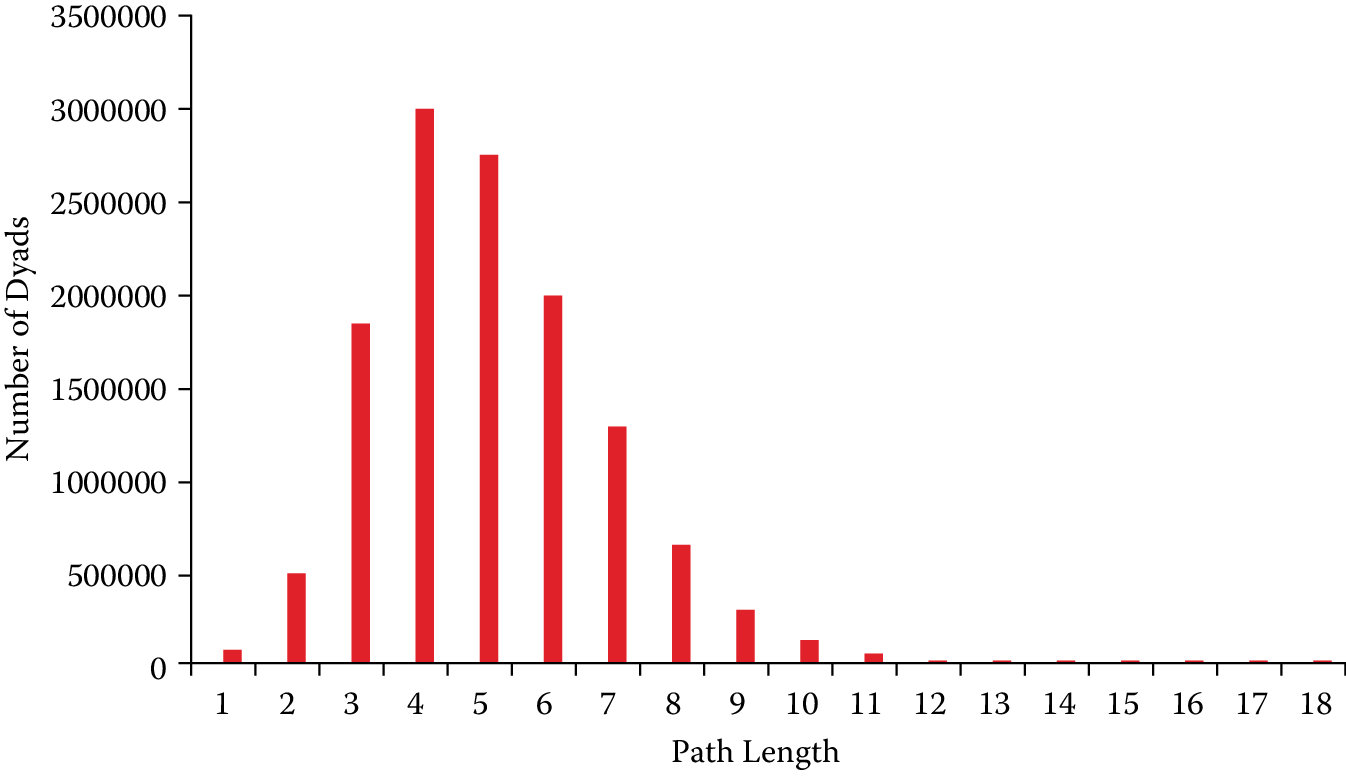
\includegraphics[width=0.7\linewidth]{ChapterNetworks/figures/fig8-5} 

}

\caption{Histogram of path lengths for university A employee network}\label{fig:fig8-5}
\end{figure}

\textbf{Degree distribution}

Another powerful way to describe and compare networks is to look at the
distribution of centralities across nodes. While any of the centrality
measures described above could be summarized in terms of their
distribution, it is most common to plot the degree distribution of large
networks. Degree distributions commonly have extremely long tails. The
implication of this pattern is that most nodes have a small number of
ties (typically one or two) and that a small percentage of nodes account
for the lion's share of a network's connectivity and reachability.
Degree distributions are typically so skewed that it is common practice
to plot degree against the percentage of nodes with that degree score on
a log--log scale.

High-degree nodes are often particularly important actors. In the
UMETRICS networks that are employee \(\times\) employee projections of
employee \(\times\) grant networks, for instance, the nodes with the
highest degree seem likely to include high-profile faculty---the
investigators on larger institutional grants such as National Institutes
of Health-funded Clinical and Translational Science Awards and National
Science Foundation-funded Science and Technology Centers, and perhaps
staff whose particular skills are in demand (and paid for) by multiple
research teams. For instance, the head technician in a core microscopy
facility or a laboratory manager who serves multiple groups might appear
highly central in the degree distribution of a UMETRICS network.

Most importantly, the degree distribution is commonly taken to provide
insight into the dynamics by which a network was created. Highly skewed
degree distributions often represent scale-free networks (Powell et al.
\protect\hyperlink{ref-powell2005network}{2005}; Barabási and Albert
\protect\hyperlink{ref-barabasi1999emergence}{1999}; Newman
\protect\hyperlink{ref-newman2005measure}{2005}), which grow in part
through a process called \emph{preferential attachment}, where new nodes
entering the network are more likely to attach to already prominent
participants. In the kinds of scientific collaboration networks that
UMETRICS represents, a scale-free degree distribution might come about
as faculty new to an institution attempt to enroll more established
colleagues on grants as coinvestigators. In the comparison exercise
outlined below, I plot degree distributions for the main components of
two different university networks.

\textbf{Clustering coefficient}

The third commonly used whole-network measure captures the extent to
which a network is cohesive, with many nodes interconnected. In networks
that are more cohesively clustered, there are fewer opportunities for
individuals to play the kinds of brokering roles that we will discuss
below in the context of betweenness centrality. Less cohesive networks,
with lower levels of clustering, are potentially more conducive to
brokerage and the kinds of innovation that accompany it.

However, the challenge of innovation and discovery is both the moment of
invention, the ``aha!'' of a good new idea, and the often complicated,
uncertain, and collaborative work that is required to turn an initial
insight into a scientific finding. While less clustered, open networks
are more likely to create opportunities for brokers to develop fresh
ideas, more cohesive and clustered networks support the kinds of
repeated interactions, trust, and integration that are necessary to do
uncertain and difficult collaborative work.

While it is possible to generate a global measure of cohesiveness in
networks, which is generically the number of closed triangles (groups of
three nodes all connected to one another) as a proportion of the number
of possible triads, it is more common to take a local measure of
connectivity and average it across all nodes in a network. This local
connectivity measure more closely approximates the notion of cohesion
around nodes that is at the heart of studies of networks as means to
coordinate difficult, risky work. The code snippet below calculates both
the global clustering coefficient and a vector of node-specific
clustering coefficients whose average represents the local measure for
the employee \(\times\) employee network projection of the university A
UMETRICS data.

\begin{Shaded}
\begin{Highlighting}[]
\CommentTok{# Calculate clustering coefficients}
\KeywordTok{emp.transitivity_undirected}\NormalTok{()}
\CommentTok{# 0.7241}

\NormalTok{local_clust=}\KeywordTok{emp.transitivity_local_undirected}\NormalTok{(}\DataTypeTok{mode=}\StringTok{"zero"}\NormalTok{)}
\CommentTok{# (isolates="zero" sets clustering to zero rather than undefined)}

\NormalTok{import pandas as pd}
\KeywordTok{print}\NormalTok{(}\KeywordTok{pd.Series}\NormalTok{(local_clust)}\KeywordTok{.describe}\NormalTok{())}
\CommentTok{# count    9206.000000}
\CommentTok{# mean        0.625161}
\CommentTok{# std         0.429687}
\CommentTok{# min         0.000000}
\CommentTok{# 25%         0.000000}
\CommentTok{# 50%         0.857143}
\CommentTok{# 75%         1.000000}
\CommentTok{# max         1.000000}
\CommentTok{#--------------------------------------------------#}
\end{Highlighting}
\end{Shaded}

\pagebreak
Together, these summary statistics---number of nodes, average path
length, distribution of path lengths, degree distribution, and the
clustering coefficient---offer a robust set of measures to examine and
compare whole networks. It is also possible to distinguish among the
positions nodes hold in a particular network. Some of the most powerful
centrality measures also rely on the idea of indirect ties\footnote{Key
  insight: Some of the most powerful centrality measures also rely on
  the idea of indirect ties.}.

\textbf{Centrality measures}

This class of measures is the most common way to distinguish between the
positions individual nodes hold in networks. There are many different
measures of centrality that capture different aspects of network
positions, but they fall into three general types. The most basic and
intuitive measure of centrality, \emph{degree centrality,} simply counts
the number of ties that a node has. In a binary undirected network, this
measure resolves into the number of unique alters each node is connected
to. In mathematical terms it is the row or column sum of the adjacency
matrix that characterizes a network. Degree centrality,
\(C_{D}(n_{i})\), represents a clear measure of the prominence or
visibility of a node. Let \[C_D(n_i)=\sum_jx_{ij}.\] The degree of a
node is limited by the size of the network in which it is embedded. In a
network of \(g\) nodes the maximum degree of any node is \(g-1\). The
two orange nodes in the small networks presented in Figure
\ref{fig:fig8-4} have the maximum degree possible (4). In contrast, the
orange node in the larger, 13-node network in that figure has the same
number of alters but the possible number of partners is three times as
large (12). For this reason it is problematic to compare raw degree
centrality measures across networks of different sizes. Thus, it is
common to normalize degree by the maximum value defined by \(g-1\):
\[C_D^{\prime}(n_i)=\frac{\sum_j x_{ij}}{g-1}.\]

While the normalized degree centrality of the two orange nodes of the
smaller networks in Figure \ref{fig:fig8-4} is 1.0, the normalized value
for the node in the large network of 13 nodes is 0.33. Despite the fact
that the highlighted nodes in the two smaller networks have the same
degree centrality, the pattern of indirect ties connecting their alters
means they occupy meaningfully different positions. There are a number
of degree-based centrality measures that take more of the structural
information from a complete network into account by using a variety of
methods to account not just for the number of partners a particular ego
might have but also for the prominence of those partners. Two well-known
examples are eigenvector centrality and page rank (see (Newman
\protect\hyperlink{ref-newman2010networks}{2010} Ch. 7.2 and 8.4)).

Consider two additional measures that capture aspects of centrality that
have more to do with the indirect ties that increase reachability. Both
make explicit use of the idea that reachability is the source of many of
the important social and economic benefits of salutary network
positions, but they do so with different substantive emphases. Both of
these approaches rely on the idea of a network geodesic, the longest
shortest path\footnote{A \emph{shortest path} is a path that does not
  repeat any nodes or ties. Most pairs have several of those. The
  \emph{geodesic} is the longest shortest path. So, if two people are
  directly connected (path length 1) and connected through shared ties
  to another person (path length 2), then their geodesic distance is
  two.} connecting any pair of actors. Because these measures rely on
reachability, they are only useful when applied to components. When
nodes have no ties (degree 0) they are called \emph{isolates}. The
geodesic distances are infinite and thus path-based centrality measures
cannot be calculated. This is a shortcoming of these measures, which can
only be used on connected subsets of graphs where each node has at least
one tie to another and all are indirectly connected.

Closeness centrality, \(C_{C,}\) is based on the idea that networks
position some individuals closer to or farther away from other
participants. The primary idea is that shorter network paths between
actors increase the likelihood of communication and with it the ability
to coordinate complicated activities. Let \(d(n_{i}, n_{j})\) represent
the number of network steps in the geodesic path connecting two nodes
\(i\) and \(j\). As \(d\) increases, the network distance between a pair
of nodes grows. Thus a standard measure of closeness is the inverse of
the sum of distances between any given node and all the others that are
reachable in a network: \[C_C(n_i) = \frac{1}{\sum_{j=1}^gd(n_i,n_j)}.\]
The maximum of closeness centrality occurs when a node is directly
connected to every possible partner in the network. As with degree
centrality, closeness depends on the number of nodes in a network. Thus,
it is necessary to standardize the measure to allow comparisons across
multiple networks:
\[C_C^{\prime}(n_i)=\frac{g-1}{\sum_{j=1}^gd(n_i,n_j)}.\]

Like closeness centrality, betweenness centrality, \(C_{B}\), relies on
the concept of geodesic paths to capture nuanced differences the
positions of nodes in a connected network. Where closeness assumes that
communication and the flow of information increase with proximity,
betweenness captures the idea of brokerage that was made famous by Burt
(Burt \protect\hyperlink{ref-burt1993social}{1993}). Here too the idea
is that flows of information and resources pass between nodes that are
not directly connected through indirect paths. The key to the idea of
brokerage is that such paths pass through nodes that can interdict, or
otherwise profit from their position ``in between'' unconnected alters.
This idea has been particularly important in network studies of
innovation (Owen-Smith and Powell
\protect\hyperlink{ref-owen2003expanding}{2003}; Burt
\protect\hyperlink{ref-burt2004structural}{2004}), where flows of
information through strategic alliances among firms or social networks
connecting individuals loom large in explanations of why some
organizations or individuals are better able to develop creative ideas
than others.

To calculate betweenness as originally specified, two strong assumptions
are required (Freeman
\protect\hyperlink{ref-freeman1979centrality}{1979}). First, one must
assume that when people (or organizations) search for new information
through their networks, they are capable of identifying the shortest
path to what they seek. When multiple paths of equal length exist, we
assume that each path is equally likely to be used. Newman (Newman
\protect\hyperlink{ref-newman2005measure}{2005}) describes an
alternative betweenness measure based on random paths through a network,
rather than shortest paths, that relaxes these assumptions. For now, let
\(g_{jk}\) equal the number of geodesic paths linking any two actors.
Then \(1/g_{jk}\) is the probability that any given path will be
followed on a particular node's search for information or resources in a
network. In order to calculate the betweenness score of a particular
actor, \(i\), it is then necessary to determine how many of the geodesic
paths connecting \(j\) to \(k\) include \(i\). That quantity is
\(g_{jk}(n_{i})\). With these (unrealistic) assumptions in place, we
calculate \(C_{B}(n_{i})\) as
\[C_B(n_i)=\sum_{j<k} g_{jk}^{(n_i)}/g_{jk}.\] Here, too, the maximum
value depends on the size of the network. \(C_{B}(n_{i}) = 1\) if \(i\)
sits on every geodesic path in the network. While this is only likely to
occur in small, star-shaped networks, it is still common to standardize
the measure. Instead of conceptualizing network size in terms of the
number of nodes, however, this measure requires that we consider the
number of possible pairs of actors (excluding ego) in a structure. When
there are \(g\) nodes, that quantity is \((g-1)(g-2)/2\) and the
standardized betweenness measure is
\[C_B^{\prime}(n_i)=\frac{C_B(n_i)}{(g-1)(g-2)/2}.\]

Centrality measures of various sorts are the most commonly used means to
examine network effects at the level of individual participants in a
network. In the context of UMETRICS, such indices might be applied to
examine the differential scientific or career success of graduate
students as a function of their positions in the larger networks of
their universities. In such an analysis, care must be taken to use the
standardized measures as university collaboration networks can vary
dramatically in size and structure. Describing and accounting for such
variations and the possibility of analyses conducted at the level of
entire networks or subsets of networks, such as teams and labs, requires
a different set of measures. The code snippet presented below calculates
each of these measures for the university A employee network we have
been examining.

\begin{Shaded}
\begin{Highlighting}[]
\CommentTok{# Calculate centrality measures}
\NormalTok{emp.vs[}\StringTok{"degree"}\NormalTok{]=}\KeywordTok{emp.degree}\NormalTok{()}
\NormalTok{emp.vs[}\StringTok{"close"}\NormalTok{]=}\KeywordTok{emp.closeness}\NormalTok{(}\DataTypeTok{vertices=}\NormalTok{emp.vs)}
\NormalTok{emp.vs[}\StringTok{"btc"}\NormalTok{]=}\KeywordTok{emp.betweenness}\NormalTok{(}\DataTypeTok{vertices=}\NormalTok{emp.vs, }\DataTypeTok{directed=}\NormalTok{False)}
\end{Highlighting}
\end{Shaded}

\section{What kinds of questions can now be
answered?}\label{what-kinds-of-questions-can-now-be-answered}

Who are the most important actors (nodes) in a network? Most connections
- degree Most central - centrality measures Most critical in connecting
two disjoint groups - bridge measure Most influential

\begin{enumerate}
\def\labelenumi{\arabic{enumi}.}
\setcounter{enumi}{1}
\tightlist
\item
  What types of relationships exist in this network? Network motifs
  (paper reference)
\end{enumerate}

\section{Case Study: Comparing collaboration
networks}\label{case-study-comparing-collaboration-networks}

Consider Figure \ref{fig:fig8-6}, which presents visualizations of the
main component of two university networks. Both of these representations
are drawn from a single year (2012) of UMETRICS data. Nodes represent
people, and ties reflect the fact that those individuals were paid with
the same federal grant in the same year. The images are scaled so that
the physical location of any node is a function of its position in the
overall pattern of relationships in the network. The size and color of
nodes represent their betweenness centrality. Larger, darker nodes are
better positioned to play the role of brokers in the network. A complete
review of the many approaches to network visualization and their dangers
in the absence of descriptive statistics such as those presented above
is beyond the scope of this chapter, but consider the guidelines
presented in Chapter \protect\hyperlink{chap:viz}{Information
Visualization} on information visualization as well as useful
discussions by Powell et al. (Powell et al.
\protect\hyperlink{ref-powell2005network}{2005}) and Healy and Moody
(Healy and Moody \protect\hyperlink{ref-healy2014data}{2014}).

Consider the two images. University A is a major public institution with
a significant medical school. University B, likewise, is a public
institution but lacks a medical school. It is primarily known for strong
engineering. The two networks manifest some interesting and suggestive
differences. Note first that the network on the left (university A)
appears much more tightly connected. There is a dense center and there
are fewer very large nodes whose positions bridge less well-connected
clusters. Likewise, the network on the right (university B) seems at a
glance to be characterized by a number of densely interconnected groups
that are pulled together by ties through high-degree brokers. One part
of this may have to do with the size and structure of university A's
medical school, whose significant NIH funding dominates the network. In
contrast, university B's engineering-dominated research portfolio seems
to be arranged around clusters of researchers working on similar topic
areas and lacks the dominant central core apparent in university B's
image.

The implications of these kinds of university-level differences are just
starting to be realized, and the UMETRICS data offer great possibilities
for exactly this kind of study. These networks, in essence, represent
the local social capacity to respond to new problems and to develop
scientific findings. Two otherwise similar institutions might have quite
different capabilities based on the structure and composition of their
collaboration networks.

\begin{figure}

{\centering 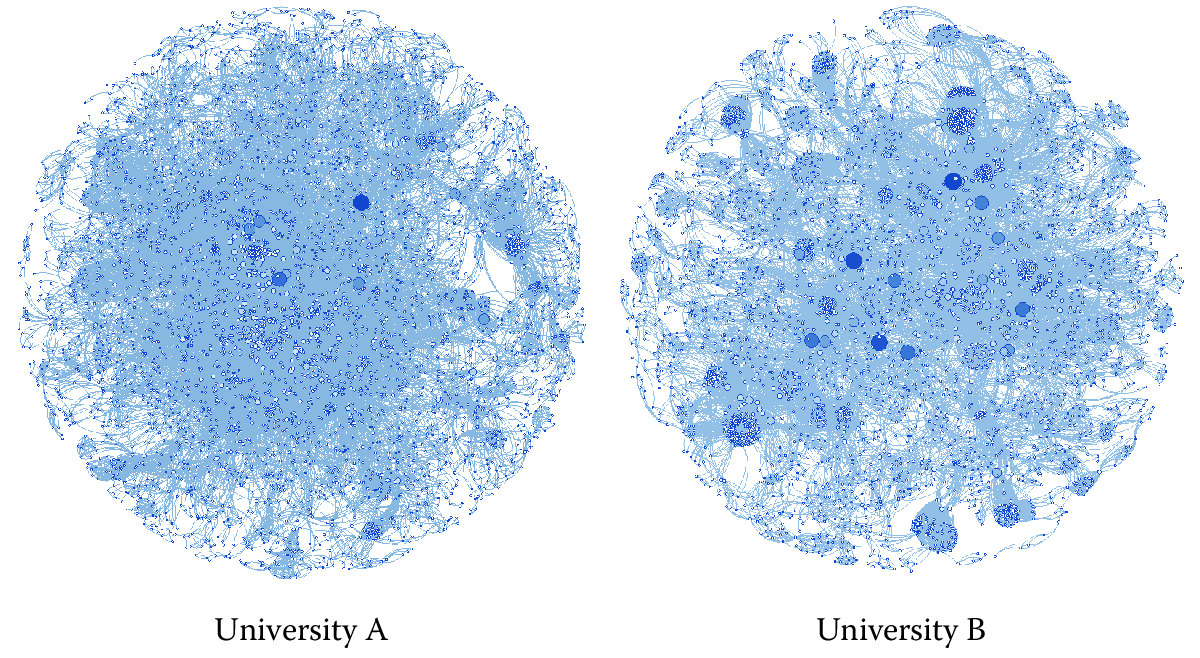
\includegraphics[width=0.7\linewidth]{ChapterNetworks/figures/fig8-6} 

}

\caption{The main component of two university networks}\label{fig:fig8-6}
\end{figure}

The intuitions suggested by Figure \ref{fig:fig8-6} can also be checked
against some of the measures we have described. Figure
\ref{fig:fig8-7a}, for instance, presents degree distributions for each
of the two networks. Figure \ref{fig:fig8-8} presents the histogram of
path lengths for each network.

\begin{center}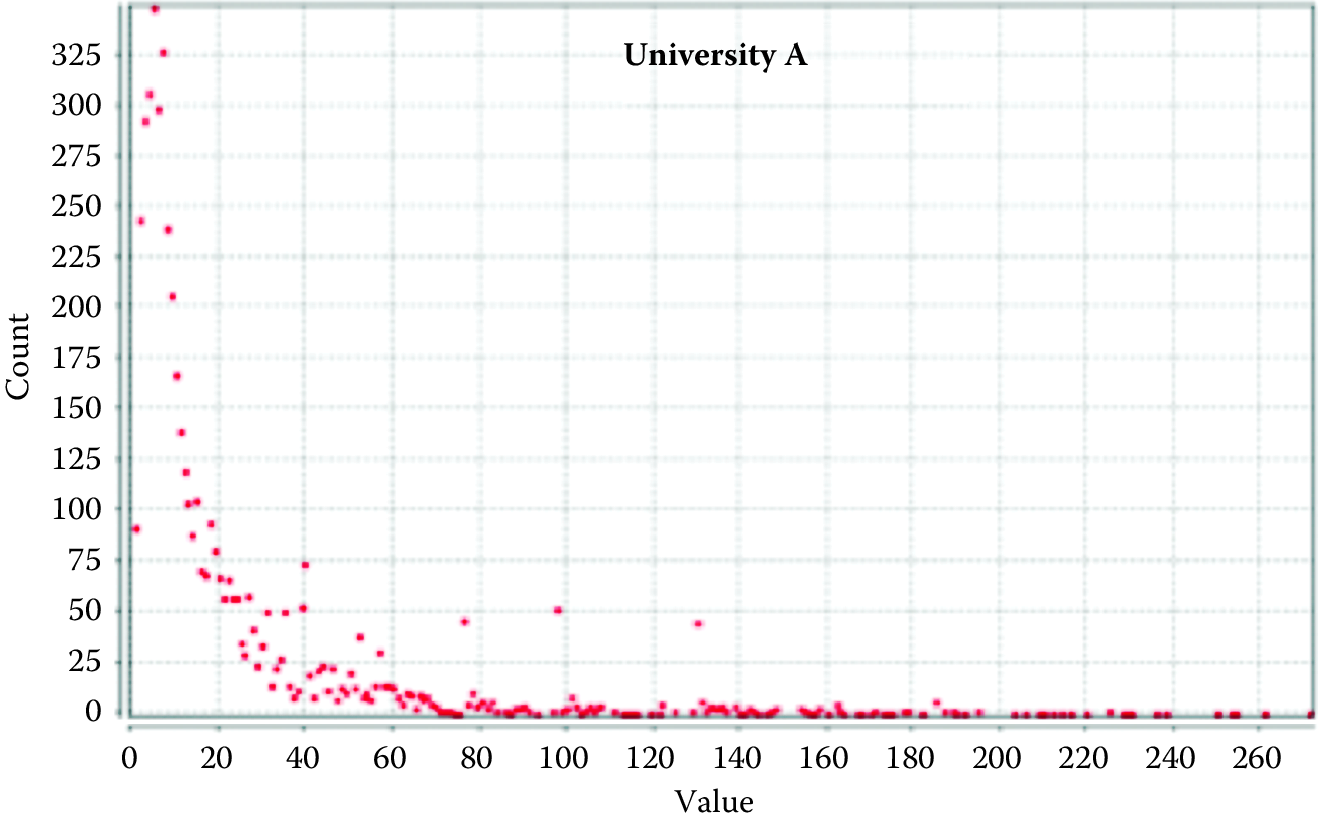
\includegraphics[width=0.7\linewidth]{ChapterNetworks/figures/fig8-7a} \end{center}\begin{figure}

{\centering 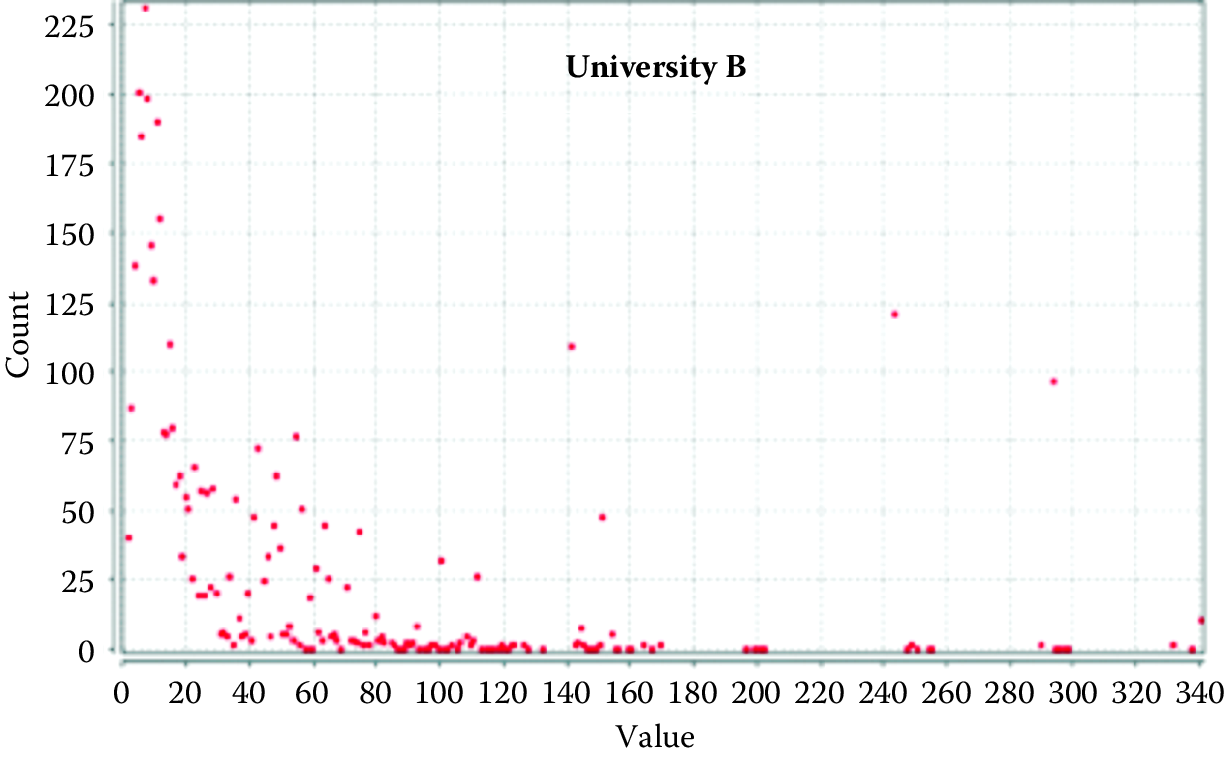
\includegraphics[width=0.7\linewidth]{ChapterNetworks/figures/fig8-7b} 

}

\caption{Degree distribution for two universities}\label{fig:fig8-7a}
\end{figure}

It is evident from Figure \ref{fig:fig8-7a} that they are quite
different in character. University A's network follows a more classic
skewed distribution of the sort that is often associated with the kinds
of power-law degree distributions common to scale- free networks. In
contrast, university B's distribution has some interesting features.
First, the left-hand side of the distribution is more dispersed than it
is for university A, suggesting that there are many nodes with moderate
degree. These nodes may also have high betweenness centrality if their
ties allow them to span different subgroups within the networks. Of
course this might also reflect the fact that each cluster also has
members that are more locally prominent. Finally, consider the few
instances on the right-hand end of the distribution where there are
relatively large numbers of people with surprisingly high degree. I
suspect these are the result of large training grants or center grants
that employ many people. A quirk of relying on one-mode projections of
two-mode data is that every person associated with a particular grant is
connected to every other. More work needs to be done to bear out these
hypotheses, but for now it suffices to say that the degree distribution
of the networks bears out the intuition we drew from the images that
they are significantly different.

\begin{figure}

{\centering 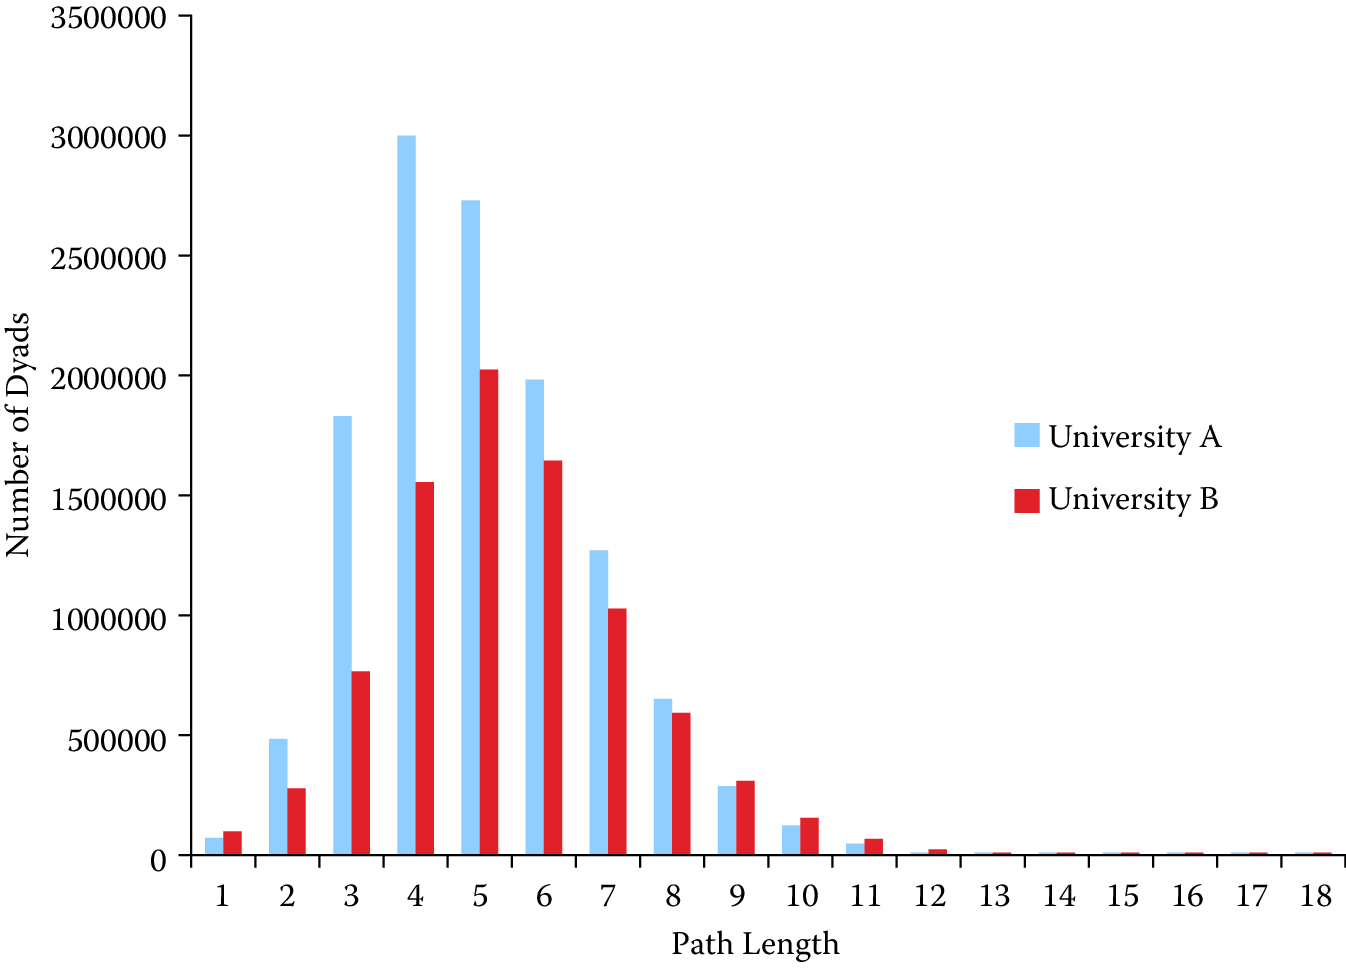
\includegraphics[width=0.7\linewidth]{ChapterNetworks/figures/fig8-8} 

}

\caption{Distribution of path lengths for universities A and B}\label{fig:fig8-8}
\end{figure}

The path length histogram presented in Figure \ref{fig:fig8-8} suggests
a similar pattern. While the average distance among any pair of
connected nodes in both networks is fairly similar (see Table
\ref{tab:table8-1}, university B has a larger number of unconnected
nodes and university A has a greater concentration of more closely
connected dyads. The preponderance of shorter paths in this network
could also be a result of a few larger grants that connect many pairs of
nodes at unit distance and thus shorten overall path lengths.

\begin{longtable}[]{@{}lcc@{}}
\caption{\label{tab:table8-1} Descriptive statistics for the main components
of two university networks}\tabularnewline
\toprule
& \textbf{University A} & \textbf{University B}\tabularnewline
\midrule
\endfirsthead
\toprule
& \textbf{University A} & \textbf{University B}\tabularnewline
\midrule
\endhead
Nodes & 4,999 & 4,144\tabularnewline
Edges (total) & 57,756 & 91,970\tabularnewline
\% nodes in main component & 68.67\% & 67.34\%\tabularnewline
Diameter & 18 & 18\tabularnewline
Average degree & 11.554 & 44.387\tabularnewline
Clustering coefficient & 0.855 & 0.913\tabularnewline
Density & 0.005 & 0.011\tabularnewline
Average path length & 5.034 & 5.463\tabularnewline
\bottomrule
\end{longtable}

But how do the descriptive statistics shake out? Table
\ref{tab:table8-1} presents the basic descriptive statistics we have
discussed for each network. University A's network includes 855 more
nodes than university B's, a difference of about 20\%. In contrast,
there are far fewer edges connecting university A's research employees
than connecting university B's, a difference that appears particularly
starkly in the much higher density of university B's network. Part of
the story can be found in the average degree of nodes in each network.
As the degree distributions presented in Figure \ref{fig:fig8-6}
suggested, the average researcher at university B is much more highly
connected to others than is the case at university A. The difference is
stark and quite likely has to do with the presence of larger grants that
employ many individuals.

Both schools have a low average path length (around 5), suggesting that
no member of the network is more than five acquaintances away from any
other. Likewise, the diameter of both networks is 18, which means that
on each campus the most distant pair of nodes is separated by just 18
steps. University A's slightly lower path length may be accounted for by
the centralizing effect of its large medical school grant
infrastructure. Finally, consider the clustering coefficient. This
measure approaches 1 as it becomes more likely that two partners to a
third node will themselves be connected. The likelihood that
collaborators of collaborators will collaborate is high on both
campuses, but substantially higher at university B.

\section{Summary}\label{summary-5}

This chapter has provided a brief overview of the basics of networks and
how to do large-scale network analysis. While network measures can
produce new and exciting ways to characterize social dynamics, they are
also important levels of analysis in their own right. Concepts such as
reachability, cohesion, brokerage, and reciprocity are important, for a
variety of reasons---they can be used to describe networks in terms of
their composition and community structure. This chapter provides a
classic example of how well social science meets data science. Social
science is needed to identify the nodes (what is being connected) and
the ties (the relationships that matter) in order to construct the
relevant networks. Computer science is necessary to collect and
structure the data in a fashion that is sufficient for analysis. The
combination of data science and social science is key to making the
right measurement and visualization decisions.

\section{Resources}\label{resources-4}

For more information about network analysis \emph{in general}, the
International Network for Social Network Analysis
(\url{http://www.insna.org/}) is a large, interdisciplinary association
dedicated to network analysis. It publishes a traditional academic
journal, \emph{Social Networks}, an online journal, \emph{Journal of
Social Structure}, and a short-format journal, \emph{Connections}, all
dedicated to social network analysis. Its several listservs offer
vibrant international forums for discussion of network issues and
questions. Finally, its annual meetings include numerous opportunities
for intensive workshops and training for both beginning and advanced
analysts.

A new journal, \emph{Network Science}
(\url{http://journals.cambridge.org/action/displayJournal?jid=NWS}),
published by Cambridge University Press and edited by a team of
interdisciplinary network scholars, is a good venue to follow for
cutting-edge articles on computational network methods and for
substantive findings from a wide range of social, natural, and
information science applications.

There are some good software packages available. \emph{Pajek}
(\url{http://mrvar.fdv.uni-lj.si/pajek/}) is a freeware package for
network analysis and visualization. It is routinely updated and has a
vibrant user group. Pajek is exceptionally flexible for large networks
and has a number of utilities that allow import of its relatively simple
file types into other programs and packages for network analysis.
\emph{Gephi} (\url{https://gephi.org/}) is another freeware package that
supports large-scale network visualization. Though I find it less
flexible than Pajek, it offers strong support for compelling
visualizations.

\emph{Snap} (\textless{}snap.cs.stanford.edu\textgreater{})

\emph{Network Workbench} (\url{http://nwb.cns.iu.edu/}) is a freeware
package that supports extensive analysis and visualization of networks.
This package also includes numerous shared data sets from many different
fields that can used to test and hone your network analytic skills.

\emph{iGraph} (\url{http://igraph.org/redirect.html}) is my preferred
package for network analysis. Implementations are available in R, in
Python, and in C libraries. The examples in this chapter were coded in
iGraph for Python.

\emph{Nexus}
(\url{http://nexus.igraph.org/api/dataset_info?format=html\&limit=10\&offset=20\&operator=or\&order=date})
is a growing repository for network data sets that includes some classic
data dating back to the origins of social science network research as
well as more recent data from some of the best-known publications and
authors in network science.

\hypertarget{chap:viz}{\chapter{Information
Visualization}\label{chap:viz}}

\textbf{M. Adil Yalcin and Catherine Plaisant}

This chapter will show you how to explore data and communicate results
so that data can be turned into interpretable, actionable information.
There are many ways of presenting statistical information that convey
content in a rigorous manner. The goal of this chapter is to present an
introductory overview of effective visualization techniques for a range
of data types and tasks, and to explore the foundations and challenges
of information visualization.

\vspace*{-6pt}

\section{Introduction}\label{sec:viz-1}

One of the most famous discoveries in science---that disease was
transmitted through germs, rather than through pollution--- resulted
from insights derived from a visualization of the location of London
cholera deaths near a water pump (Snow
\protect\hyperlink{ref-snow1855mode}{1855}). Information visualization
in the twenty-first century can be used to generate similar insights:
detecting financial fraud, understanding the spread of a contagious
illness, spotting terrorist activity, or evaluating the economic health
of a country. But the challenge is greater: many
(\(10^{2}\)--\(10^{7}\)) items may be manipulated and visualized, often
extracted or aggregated from yet larger data sets, or generated by
algorithms for analytics.

Visualization tools can organize data in a meaningful way that lowers
the cognitive and analytical effort required to make sense of the data
and make data-driven decisions. Users can scan, recognize, understand,
and recall visually structured representations more rapidly than they
can process nonstructured representations. The science of visualization
draws on multiple fields such as perceptual psychology, statistics, and
graphic design to present information, and on advances in rapid
processing and dynamic to design user interfaces that permit powerful
interactive visual

Figure~\ref{fig:fig9-1}, ``Anscombe's quartet'' (Anscombe
\protect\hyperlink{ref-anscombe1973graphs}{1973}), provides a classic
example of the value of visualization compared to basic descriptive
statistical analysis. The left-hand panel includes raw data of four
small number-pair data sets (A, B, C, D), which have the same average,
median, and standard deviation and have correlation across number pairs.
The right-hand panel shows these data sets visualized with each point
plotted on perpendicular axes (scatterplots), revealing dramatic
differences between the data sets, trends, and outliers visually.

\begin{figure}

{\centering 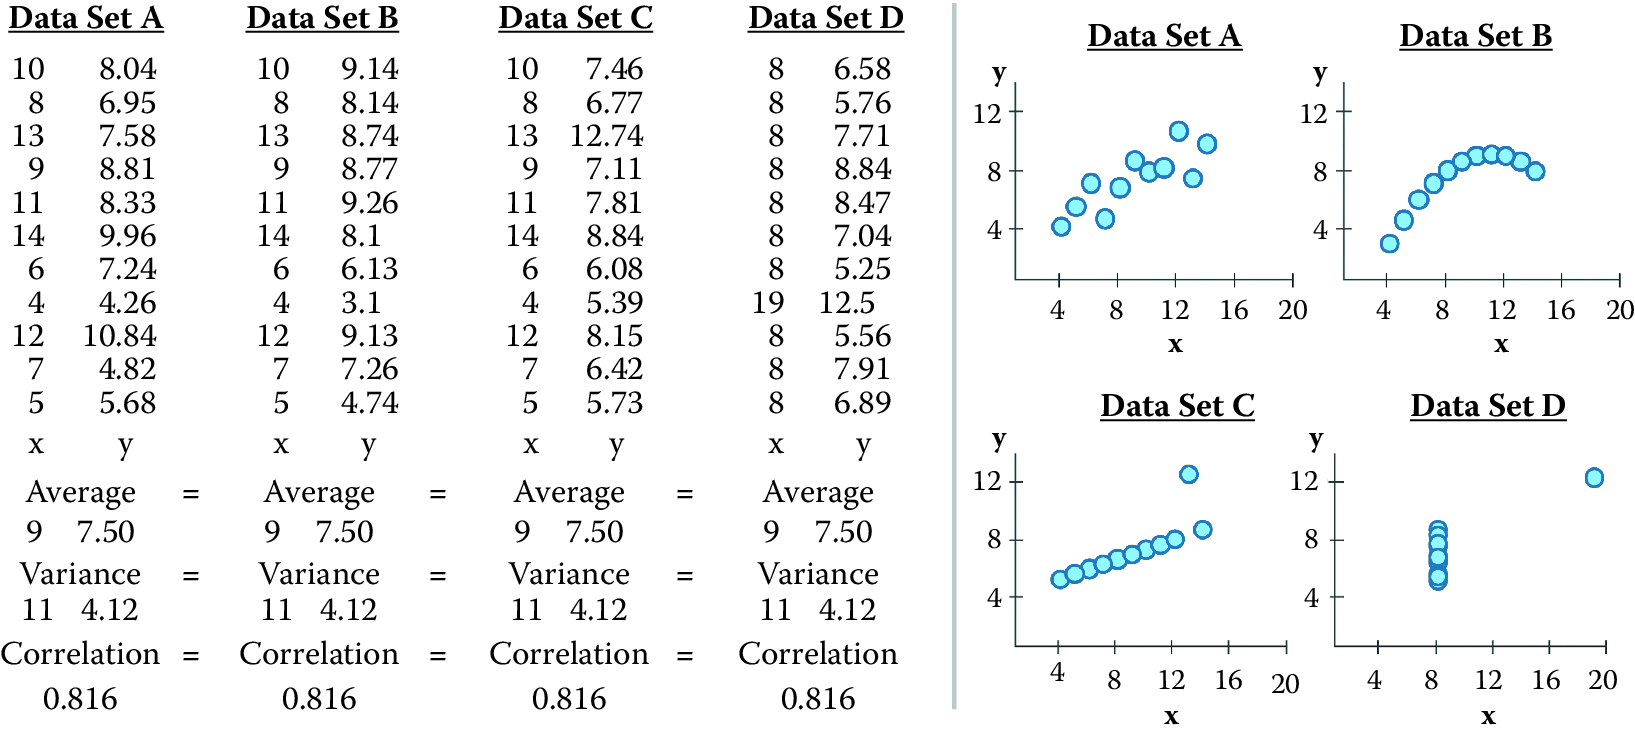
\includegraphics[width=0.7\linewidth]{ChapterViz/figures/fig9-1} 

}

\caption{Anscombes quartet [@anscombe1973graphs]}\label{fig:fig9-1}
\end{figure}

In broad terms, visualizations are used either to present results or for
analysis and open-ended exploration. This chapter provides an overview
of how modern information visualization, or visual data mining, can be
used to in the context of big data.

\section{Developing effective visualizations}\label{sec:viz-2}

The effectiveness of a visualization depends on both analysis needs and
design goals. Sometimes, questions about the data are known in advance;
in other cases, the goal may be to explore new data sets, generate
insights, and answer questions that are unknown before starting the
analysis. The design, development, and evaluation of a visualization is
guided by understanding the background and goals of the target audience
(see Box 9.1\footnote{See Chapters 2, 3, 4, and 5 for an overview of
  collecting, merging, storing, and processing data sets.}).

\begin{F00}
\textbf{Box 9.1:} The development of an effective visualization is an
iterative process that generally includes the following steps:

\begin{itemize}
\item
  Specify user needs, tasks, accessibility requirements and criteria for
  success.
\item
  Prepare data (clean, transform).
\item
  Design visual representations.
\item
  Design interaction.
\item
  Plan sharing of insights, provenance.
\item
  Prototype/evaluate, including usability testing.
\item
  Deploy (monitor usage, provide user support, manage revision process).
\end{itemize}
\end{F00}

If the goal is to present results, there is a wide spectrum of users and
a wide range of options. If the audience is broad, then
\emph{infographics} can be developed by graphic designers, as described
in classic texts (see (Few \protect\hyperlink{ref-few2009now}{2009};
Tufte \protect\hyperlink{ref-edward2001visual}{2001}; Tufte
\protect\hyperlink{ref-edward2006beauty}{2006}) or the examples compiled
by Harrison et al.~(Harrison, Reinecke, and Chang
\protect\hyperlink{ref-harrison2015infographic}{2015}; Keshif, n.d.)).
If, on the other hand, the audience comprises domain experts interested
in monitoring the overview status of dynamic processes on a continuous
basis, \emph{dashboards} can be used. Examples include the monitoring of
sales, or the number of tweets about people, or symptoms of the flu and
how they compare to a baseline (Few
\protect\hyperlink{ref-few2013information}{2013}). Dashboards can
increase situational awareness so that problems can be noticed and
solved early and better decisions can be made with up-to-date
information.

Another goal of visualization is to enable \emph{interactive exploratory
analysis} for casual users as well as professional analysts. One casual
example is BabyNameVoyager (Harrison, Reinecke, and Chang, n.d.), which
lets users type in a name and see a graph of its popularity over the
past century\footnote{As the baby name is typed letter by letter,
  BabyNameVoyager visualizes the popularity of all the names starting
  with the letters entered so far, and it animates smoothly with each
  new letter input. For example, typing ``Jo'' shows all the names
  starting with ``Jo''. This view reveals that Joyce and Joan were
  popular girl names in the 1930s, and the use of ``John'' has declined
  since the 1960s.}.

\begin{figure}

{\centering 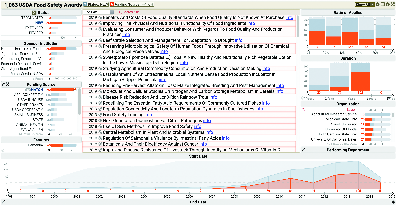
\includegraphics[width=0.7\linewidth]{ChapterViz/figures/fig9-2} 

}

\caption{A data analysis browser of a selection of grants from the US Department of Agriculture was created by using the web-based tool Keshif}\label{fig:fig9-2}
\end{figure}

\vspace*{-12pt} Data analysis tools can enable analysis of structured
and generic data sets. Figure~\ref{fig:fig9-2} shows an exploratory
browser of a selection of awards (grants) from the US Department of
Agriculture, created using the web-based data exploration tool Keshif
(\url{http://www.keshif.me}). The awards (records) are listed in the
middle panel by latest start date first. Attributes of the awards, such
as funding source, are shown on side panels, revealing the range of
their values. The awards with status \emph{new} are focused per the
filtering selection, and are visualized using darker gray colors.
Lighter gray colors provide visual cues to the distribution of all
awards. The orange selection highlights distributions of awards with
formula funding, known as \emph{Hatch funding}. The analyst can explore
trends in new or old awards, funding resources, and other attributes in
this rich award portfolio.

\begin{figure}

{\centering 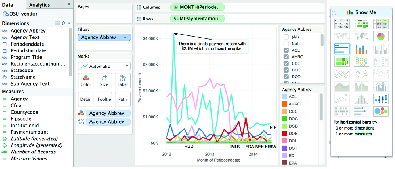
\includegraphics[width=0.7\linewidth]{ChapterViz/figures/fig9-3a} 

}

\caption{Charting interface of Tableau}\label{fig:fig9-3a}
\end{figure}

\begin{figure}

{\centering 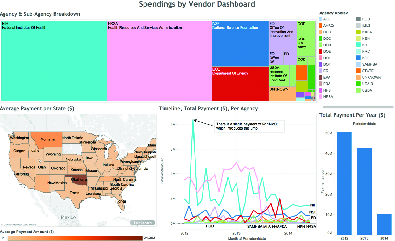
\includegraphics[width=0.7\linewidth]{ChapterViz/figures/fig9-3b} 

}

\caption{A treemap visualization of agency and sub-agency spending breakdown}\label{fig:fig9-3b}
\end{figure}

Commercial tools such as Spotfire and Tableau, among many other tools
(see Section~\protect\hyperlink{sec:mylabel4}{Resources}), allow users
to create visualizations by offering chart types and visual design
environments to analyze their data, and to combine them in potent
dashboards rapidly shared with colleagues. For example, Figure
\ref{fig:fig9-3a} shows the charting interface of Tableau on a
transaction data set. The left-hand panel shows the list of attributes
associated with vendor transactions for a given university. The
visualization (center) is constructed by placing the month of spending
in chart columns, and the sum of payment amount on the chart row, with
data encoded using line mark type. Agencies are broken down by color
mapping. The agency list, to the right, allows filtering the agencies,
which can be used to simplify the chart view. A peak in the line chart
is annotated with an explanation of the spike. On the rightmost side,
the Show Me panel suggests the applicable chart types potentially
appropriate for the selected attributes. This chart can be combined with
other charts focusing on other aspects in interactive dashboards.
Figure~\ref{fig:fig9-3b} shows a treemap (Johnson and Shneiderman
\protect\hyperlink{ref-johnson1991tree}{1991}) for agency and sub-agency
spending breakdown, combined with a map showing average spending per
state. Oklahoma state stands out with few but large expenditures.
Mousing-over Oklahoma reveals details of these expenditures. An
additional histogram provides an overview of spending change across
three years.

Creating effective visualizations requires careful consideration of many
components. Data values may be encoded using one or more visual
elements, like position, length, color, angle, area, and texture (Figure
\ref{fig:fig9-4}; see also (Cleveland and McGill
\protect\hyperlink{ref-cleveland1984graphical}{1984}; Tufte
\protect\hyperlink{ref-edward2001visual}{2001})). Each of these can be
organized in a multitude of ways, discussed in more detail by Munzner
(Munzner \protect\hyperlink{ref-munzner2014visualization}{2014}). In
addition to visual data encoding, units for axes, labels, and legends
need to be provided as well as explanations of the mappings when the
design is unconventional. (The website ``A World of Terror'' provides
some compelling examples (PERISCOPIC, n.d.).) Annotations or comments
can be used to guide viewer attention and to describe related insights.
Providing attribution and data source, where applicable, is an ethical
practice that also enables validating data, and promotes reuse to
explore new perspectives.

\begin{figure}

{\centering 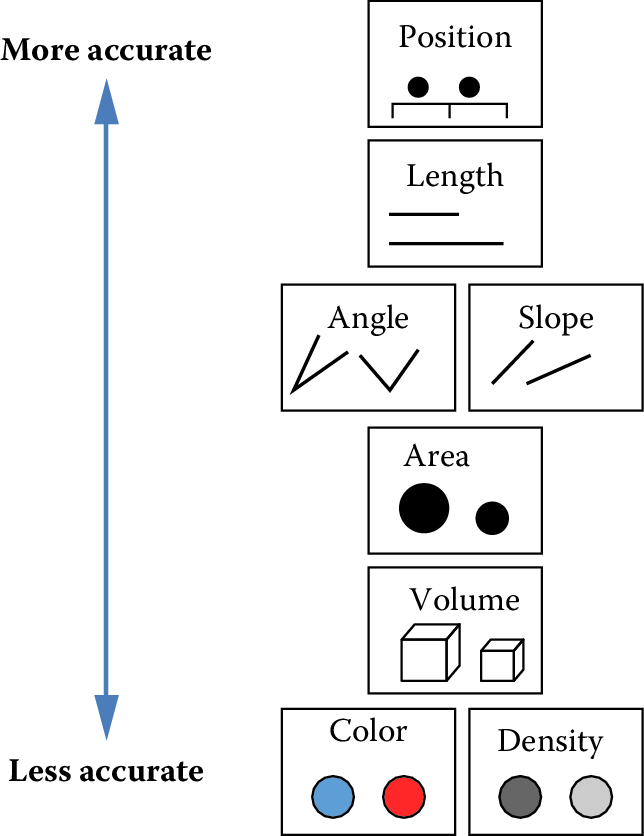
\includegraphics[width=0.7\linewidth]{ChapterViz/figures/fig9-4} 

}

\caption{Visual elements described by MacKinlay [@mackinlay1986automating]}\label{fig:fig9-4}
\end{figure}

\vspace*{-8pt} The following is a short list of guidelines: provide
immediate feedback upon interaction with the visualization; generate
tightly coupled views (i.e., so that selection in one view updates the
others); and use a high ``data to ink ratio'' (Tufte
\protect\hyperlink{ref-edward2001visual}{2001}). Use color carefully and
ensure that the visualization is truthful (e.g., watch for perceptual
biases or distortion). Avoid use of three-dimensional representations or
embellishments, since comparing 3D volumes is perceptually challenging
and occlusion is a problem. Labels and legends should be meaningful,
novel layouts should be carefully explained, and online visualizations
should adapt to different screen sizes. For extended and in-depth
discussions, see various textbooks (Few
\protect\hyperlink{ref-few2009now}{2009}; Kirk
\protect\hyperlink{ref-kirk2012data}{2012}; Ward, Grinstein, and Keim
\protect\hyperlink{ref-ward2010interactive}{2010}; Munzner
\protect\hyperlink{ref-munzner2014visualization}{2014}; Tufte
\protect\hyperlink{ref-edward2001visual}{2001}; Tufte
\protect\hyperlink{ref-edward2006beauty}{2006}).

We provide a summary of the basic tasks that users typically perform
during visual analysis of data in the next section.

\vspace*{-3pt}

\section{A data-by-tasks taxonomy}\label{sec:viz-3}

We give an overview of visualization approaches for six common data
types: multivariate, spatial, temporal, hierarchical, network, and text
(Shneiderman and Plaisant
\protect\hyperlink{ref-shneiderman2015sharpening}{2015}). For each data
type listed in this section, we discuss its distinctive properties, the
common analytical questions, and examples. Real-life data sets often
include multiple data types coming from multiple sources. Even a single
data source can include a variety of data types. For example, a single
data table of countries (as rows) can have a list of attributes with
varying types: the growth rate in the last 10 years (one observation per
year, time series data), their current population (single numerical
data), the amount of trade with other countries (networked/linked data),
and the top 10 exported products (if grouped by industry, hierarchical
data). Furthermore, we provide an overview of common tasks for visual
data analysis in Box 9.2, which can be applied across different data
types based on goals and types of visualizations.

\begin{F00}
\textbf{Box 9.2: A task categorization for visual data analysis}

Select/Query

\begin{itemize}
\item
  Filter to focus on a subset of the data
\item
  Retrieve details of item
\item
  Brush linked selections across multiple charts
\item
  Compare across multiple selections
\end{itemize}

Navigate

\begin{itemize}
\item
  Scroll along a dimension (1D)
\item
  Pan along two dimensions (2D)
\item
  Zoom along the third dimension (3D)
\end{itemize}

Derive

\begin{itemize}
\item
  Aggregate item groups and generate characteristics
\item
  Cluster item groups by algorithmic techniques
\item
  Rank items to define ordering
\end{itemize}

Organize

\begin{itemize}
\item
  Select chart type and data encodings to organize data
\item
  Layout multiple components or panels in the interface
\end{itemize}

Understand

\begin{itemize}
\item
  Observe distributions
\item
  Compare items and distributions
\item
  Relate items and patterns
\end{itemize}

Communicate

\begin{itemize}
\item
  Annotate findings
\item
  Share results
\item
  Trace action histories
\end{itemize}
\end{F00}

Interactive visualization design is also closely coupled with the
targeted devices. Conventionally, visualizations have been designed for
mouse and keyboard interaction on desktop computers. However, a wider
range of device forms, such as mobile devices with small displays and
touch interaction, is becoming common. Creating visualizations for new
forms requires special care, though basic design principles such as
``less is more'' still apply.

\vspace*{-3pt}

\subsection{Multivariate data}\label{sec:viz-2.1}

In common tabular data, each record (row) has a list of attributes
(columns), whose value is mostly categorical or numerical. The analysis
of multivariate data with basic categorical and interval types aims to
understand patterns within and across data Given a larger number of
attributes, one of the challenges in data exploration and analytics is
to select the attributes and relations to focus on. Expertise in the
data domain can be helpful for targeting relevant attributes.

Multivariate data can be presented in multiple forms of charts depending
on the data and relations being explored. One-dimensional (1D) charts
present data on a single axis only. An example is a \emph{box-plot},
which shows quartile ranges for numerical data. So-called 1.5D charts
list the range of possible values on one axis, and describe a
measurement of data on the other. \emph{Bar charts} are a ubiquitous
example, in order to show, for example, a numeric grade per student, or
grade average for aggregated student groups by gender. Records can also
be grouped over numerical ranges, and bars can show the number of items
in each grouping, which generates a \emph{histogram} chart.
Two-dimensional charts plot data along two attributes, such as
\emph{scatterplots}. Matrix (grid) charts can also be used to show
relations between two attributes. \emph{Heatmaps} visualize each matrix
cell using color to represent its value. \emph{Correlation matrices}
show the relation between attribute pairs.

To show relations of more than two attributes (3D+), one option is to
use additional visual encodings in a single chart, for example, by
adding point size/shape as a data variable in scatterplots. Another
option is to use alternative visual designs that can encode multiple
relations within a single chart. For example, a \emph{parallel
coordinate plot} (Inselberg \protect\hyperlink{ref-inselberg2009}{2009})
has multiple parallel axes, each one representing an attribute; each
record is shown as connected lines passing through the record's values
on each attribute. Charts can also show part-of-whole relations using
appropriate mappings based on subdividing the chart space, such as
stacked charts or pie charts.

Finally, another approach to analyzing multidimensional data is to use
clustering algorithms to identify similar items. Clusters are typically
represented as a tree structure (see
Section~\protect\hyperlink{sec:viz-2.5}{Hierarchical data}). For
example, \(k\)-means clustering starts by users specifying how many
clusters to create; the algorithm then places every item into the most
appropriate cluster. Surprising relationships and interesting outliers
may be identified by these techniques on mechanical analysis algorithms.
However, such results may require more effort to interpret.

\subsection{Spatial data}\label{sec:viz-2.2}

Spatial data convey a physical context, commonly in a 2D space, such as
geographical maps or floor plans. Several of the most examples of
information visualization include maps, from the 1861 representation of
Napoleon's ill-fated Russian campaign by Minard (popularized by Tufte
(Tufte \protect\hyperlink{ref-edward2001visual}{2001}) and Kraak (Kraak
\protect\hyperlink{ref-Kraak2014}{2014})) to the interactive HomeFinder
application that introduced the concept of dynamic queries (Ahlberg,
Williamson, and Shneiderman
\protect\hyperlink{ref-ahlberg1992dynamic}{1992}). The tasks include
finding adjacent items, regions containing certain items or with
specific characteristics, and paths between items---and performing the
basic tasks listed in Box 9.1.

The primary form of visualizing spatial data is \emph{maps}. In
\emph{choropleth maps}, color encoding is used to add represent one data
attribute. \emph{Cartograms} aim to encode the attribute value with the
size of regions by distorting the underlying physical space. \emph{Tile
grid maps} reduce each spatial area to a uniform size and shape (e.g., a
square) so that the color-coded data are easier to observe and compare,
and they arrange the tiles to approximate the neighbor relations between
physical locations (DeBelius \protect\hyperlink{ref-DeBelius2015}{2015};
Stanford Visualization Group, n.d.). Grid maps also make selection of
smaller areas (such as small cities or states) easier. \emph{Contour
(isopleth) maps} connect areas with similar measurements and color each
one separately. \emph{Network maps} aim to show network connectivity
between locations, such as flights to/from many regions of the world.
Spatial data can be also presented with a nonspatial emphasis (e.g., as
a hierarchy of continents, countries, and cities).

\begin{figure}

{\centering 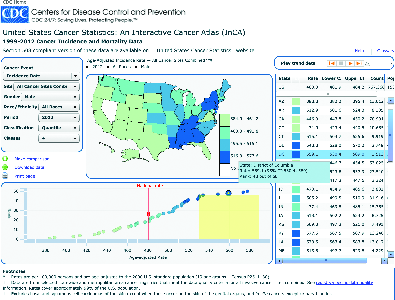
\includegraphics[width=0.7\linewidth]{ChapterViz/figures/fig9-5} 

}

\caption{The US Cancer Atlas [@usca]. Interface based on [@maceachren2008design]}\label{fig:fig9-5}
\end{figure}

Maps are commonly combined with other visualizations. For example, in
Figure~\ref{fig:fig9-5}, the US Cancer Atlas combines a map showing
patterns across states on one attribute, with a sortable table providing
additional statistical information and a scatterplot that allows users
to explore correlations between attributes.

\subsection{Temporal data}\label{sec:viz-2.4}

Time is the unique dimension in our physical world that steadily flows
forward. While we cannot control time, we frequently record it as a
point or interval. Time has multiple levels of representation (year,
month, day, hour, minute, and so on) with irregularities (leap year,
different days per month, etc.). As we measure time based on cyclic
events in nature (day/night), our representations are also commonly
cyclic. For example, January follows December (first month follows
last). This cyclic nature can be captured by circular visual encodings,
such as the the conventional clock with hour, minute, and second hands.

Time series data (Figures~\ref{fig:fig9-6} and \ref{fig:fig9-7})
describe values measured at regular intervals, such as stock market or
weather data. The focus of analysis is to understand temporal trends and
anomalies, querying for specific patterns, or prediction. To show
multiple time-series trends across different data categories in a very
compact chart area, each trend can be shown with small height using a
multi-layered color approach, creating horizon graphs. While
perceptually effective after learning to read its encoding, this chart
design may not be appropriate for audiences who may lack such training
or familiarity.

\begin{figure}

{\centering 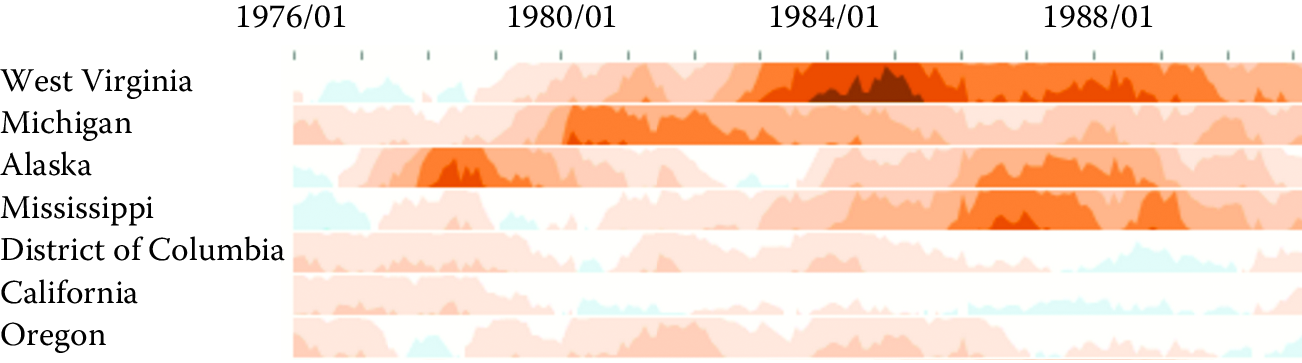
\includegraphics[width=0.7\linewidth]{ChapterViz/figures/fig9-6} 

}

\caption{Horizon graphs used to display time series}\label{fig:fig9-6}
\end{figure}

\begin{figure}

{\centering 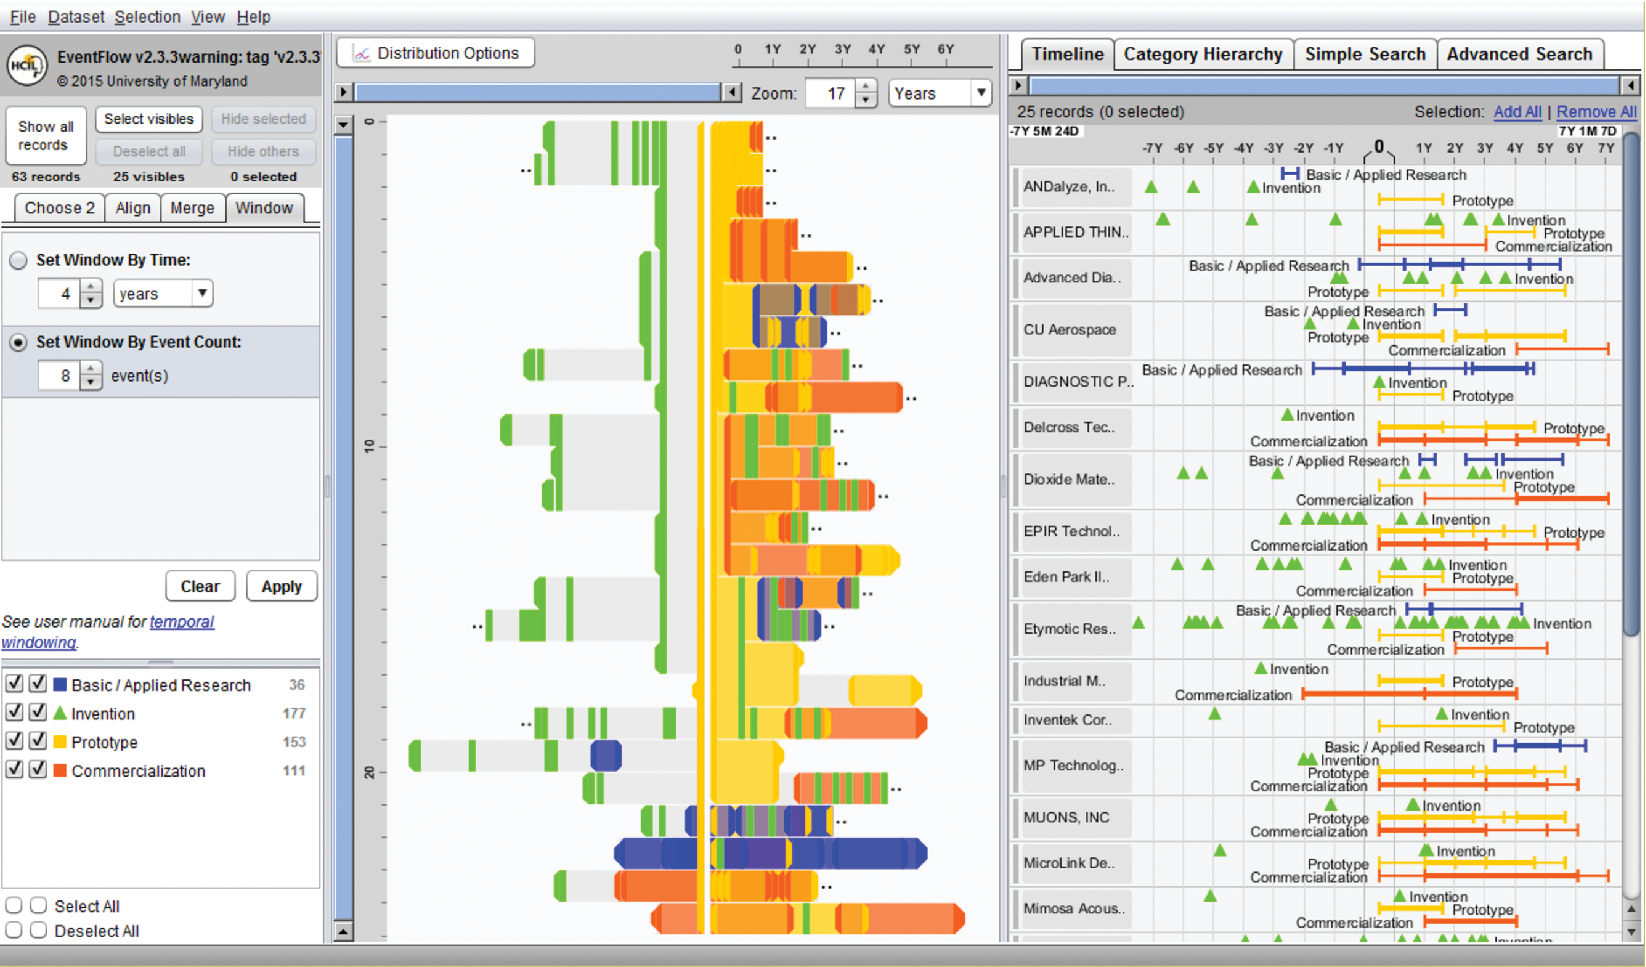
\includegraphics[width=0.7\linewidth]{ChapterViz/figures/fig9-7} 

}

\caption{EventFlow (www.cs.umd.edu/hcil/eventflow) is used to visualize sequences of innovation activities by Illinois companies. Created with EventFlow; data sources include NIH, NSF, USPTO, SBIR. Image created by C. Scott Dempwolf, used with permission}\label{fig:fig9-7}
\end{figure}

Another form of temporal analysis is understanding sequences of events.
The study of human activity often includes analyzing event sequences.
For example, students' records include events such as attending
orientation, getting a grade in a class, going on internship, and
graduation. In the analysis of event sequences, finding the most common
patterns, spotting rare ones, searching for specific sequences, or
understanding what leads to particular types of events is important
(e.g., what events lead to a student dropping out, precede a medical
error, or a company filing bankruptcy). Figure~\ref{fig:fig9-7} shows
EventFlow used to visualize sequences of innovation activities by
Illinois companies. Activity types include research, invention,
prototyping, and commercialization. The timeline (right panel) shows the
sequence of activities for each company. The overview panel (center)
summarizes all the records aligned by the first prototyping activity of
the company. In most of the sequences shown here, the company's first
prototype is preceded by two or more patents with a lag of about a year.

\enlargethispage{12pt}

\hypertarget{sec:viz-2.5}{\subsection{Hierarchical
data}\label{sec:viz-2.5}}

Data are often organized in a hierarchical fashion. Each item appears in
one grouping (e.g., like a file in a folder), and groups can be grouped
to form larger groups (e.g., a folder within a folder), up to the root
(e.g., a hard disk). Items, and the relations between items and their
grouping, can have their own attributes. For example, the National
Science Foundation is organized into directorates and divisions, each
with a budget and a number of grant recipients.

Analysis may focus on the structure of the relations, by questions such
as ``how deep is the tree?'', ``how many items does this branch have?'',
or ``what are the characteristics of one branch compared to another?''
In such cases, the most appropriate representation is usually a
node-link diagram (Plaisant, Grosjean, and Bederson
\protect\hyperlink{ref-plaisant2002spacetree}{2002}; Card and Nation
\protect\hyperlink{ref-card2002degree}{2002}). In
Figure~\ref{fig:fig9-8}, Spacetree is used to browse a company
organizational chart. Since not all the nodes of the tree fit on the
screen, we see an iconic representation of the branches that cannot be
displayed, indicating the size of each branch. As the tree branches are
opened or closed, the layout is updated with smooth multiple-step
animations to help users remain oriented.

When the structure is less important but the attribute values of the
leaf nodes are of primary interest, treemaps, a space-filling approach,
are preferable as they can show arbitrary-sized trees in a fixed
rectangular space and map one attribute to the size of each rectangle
and another to color. For example, Figure~\ref{fig:fig9-9} shows the
Finviz treemap that helps users monitor the stock market. Each stock is
shown as a rectangle. The size of the rectangle represents market
capitalization, and color indicates whether the stock is going up or
down. Treemaps are effective for situation awareness: we can see that
today is a fairly bad day as most stocks are red (i.e., down). Stocks
are organized in a hierarchy of industries, allowing users to see that
``healthcare technology'' is not doing as poorly as most other
industries. Users can also zoom on healthcare to focus on that industry.

\begin{figure}

{\centering \includegraphics[width=0.7\linewidth]{ChapterViz/figures/fig9-8} 

}

\caption{SpaceTree (www.cs.umd.edu/hcil/spacetree/)}\label{fig:fig9-8}
\end{figure}

\begin{figure}

{\centering \includegraphics[width=0.7\linewidth]{ChapterViz/figures/fig9-9} 

}

\caption{The Finviz treemap helps users monitor the stock market (www.finviz.com)}\label{fig:fig9-9}
\end{figure}

\subsection{Network data}\label{sec:viz-2.6}

\begin{figure}

{\centering \includegraphics[width=0.7\linewidth]{ChapterViz/figures/fig9-10} 

}

\caption{NodeXL showing innovation networks of the Great Lakes manufacturing region. Created with NodeXL. Data source: USPTO. Image created by C. Scott Dempwolf, used with permission}\label{fig:fig9-10}
\end{figure}

\vspace*{12pt} Network data encode relationships between items\footnote{See
  Chapter 8.}: for example, social connection patterns (friendships,
follows and reposts, etc.), travel patterns (such as trips between metro
stations), and communication patterns (such as emails). The network
overviews attempt to reveal the structure of the network, show clusters
of related items (e.g., groups of tightly connected people), and allow
the path between items to be traced. Analysis can also focus on
attributes of the items and the links in between, such as age of people
in communication or the average duration of communications.

\begin{figure}

{\centering \includegraphics[width=0.7\linewidth]{ChapterViz/figures/fig9-10b} 

}

\caption{An example from "Maps of Science: Forecasting Large Trends in Science," 2007, The Regents of the University of California, all rights reserved [@borner2010atlas]}\label{fig:fig9-10b}
\end{figure}

\vspace*{12pt} {Node-link diagrams} are the most common representation
of network structures and overviews (Figures \ref{fig:fig9-10} and
\ref{fig:fig9-10b}, and may use linear (arc), circular, or force-
directed layouts for positioning the nodes (items). Matrices or grid
layouts are also a valuable way to represent networks (Henry and Fekete
\protect\hyperlink{ref-henry2006matrixexplorer}{2006}). Hybrid solutions
have been proposed, with powerful ordering algorithms to reveal clusters
(Hansen, Shneiderman, and Smith
\protect\hyperlink{ref-hansen2010analyzing}{2010}). A major challenge in
network data exploration is in dealing with larger networks where nodes
and edges inevitably overlap by virtue of the underlying network
structure, and where aggregation and filtering may be needed before
effective overviews can be presented to users.

Figure~\ref{fig:fig9-10} shows the networks of inventors (white) and
companies (orange) and their patenting connections (purple lines) in the
network visualization NodeXL. Each company and inventor is also
connected to a location node (blue = USA; yellow = Canada). Green lines
are weak ties based on patenting in the same class and subclass, and
they represent potential economic development leads. The largest of the
technology clusters are shown using the \emph{group-in-a-box} layout
option, which makes the clusters more visible. Note the increasing level
of structure moving from the cluster in the lower right to the main
cluster in the upper left. NodeXL is designed for interactive network
exploration; many controls (not shown in the figure) allow users to zoom
on areas of interest or change options. Figure~\ref{fig:fig9-10b} shows
an example of network visualization on science as a topic used for data
presentation in a book and a traveling exhibit. Designed for print
media, it includes a clear title and annotations and shows a series of
topic clusters at the bottom with a summary of the insights gathered by
analysts.

\vspace*{6pt}

\subsection{Text data}\label{sec:viz-2.7}

Text is usually preprocessed (for word/paragraph counts, sentiment
analysis, categorization, etc.) to generate metadata about text
segments, which are then visualized\footnote{See Chapter 7 for text
  analysis approaches.}. Simple visualizations like tag clouds display
statistics about word usage in a text collection, or can be used to
compare two collections or text segments. While visually appealing, they
can easily be misinterpreted and are often replaced by word indexes
sorted by some count of interest. Specialized visual text analysis tools
combine multiple visualizations of data extracted from the text
collections, such as matrices to see relations, network diagrams, or
parallel coordinates to see entity relationships (e.g., between what,
who, where, and when). Timelines can be mapped to the linear dimension
of text. Figure~\ref{fig:fig9-11} shows an example using Jigsaw (Stasko,
Görg, and Liu \protect\hyperlink{ref-stasko2008jigsaw}{2008}) for the
exploration of car reviews. Entities have been extracted automatically
(in this case make, model, features, etc.), and a cluster analysis has
been performed, visualized in the bottom right. A separate view
(rightmost) allows analysts to review links between entities. Another
view allows traversing word sequences as a tree. Reading original
documents is critical, so all the visualization elements are linked to
the corresponding text.

\begin{figure}

{\centering \includegraphics[width=0.7\linewidth]{ChapterViz/figures/fig9-11} 

}

\caption{Jigsaw used to explore a collection of car reviews}\label{fig:fig9-11}
\end{figure}

\vspace*{6pt}

\section{Challenges}\label{sec:viz-4}

While information visualization is a powerful tool, there are many
obstacles to its effective use. We note here four areas of particular
concern: scalability, evaluation, visual impairment, and visual
literacy.

\subsection{Scalability}\label{sec:viz-4.1}

Most visualizations handle relatively small data sets (between a
thousand and a hundred thousand, sometimes up to millions, depending on
the technique) but scaling visualizations from millions to billions of
records does require careful coordination of analytic algorithms to
filter data or perform rapid aggregation, effective visual summary
designs, and rapid refreshing of displays (Shneiderman
\protect\hyperlink{ref-shneiderman2008extreme}{2008}). The visual
information seeking mantra, ``Overview first, zoom and filter, then
details on demand,'' remains useful with data at scale. To accommodate a
billion records, aggregate markers (which may represent thousands of
records) and density plots are useful (Dunne and Shneiderman
\protect\hyperlink{ref-dunne2013motif}{2013}). In some cases the large
volume of data can be aggregated meaningfully into a small number of
pixels. One example is Google Maps and its visualization of road
conditions. A quick glance at the map allows drivers to use a highly
aggregated summary of the speed of a large number of vehicles and only a
few red pixels are enough to decide when to get on the road.

While millions of graphic elements may be represented on large screens
(Fekete and Plaisant
\protect\hyperlink{ref-fekete2002interactive}{2002}), perception issues
need to be taken into consideration (Yost, Haciahmetoglu, and North
\protect\hyperlink{ref-yost2007beyond}{2007}). Extraction and filtering
may be necessary before even attempting to visualize individual records
(Wongsuphasawat and Lin
\protect\hyperlink{ref-wongsuphasawat2014using}{2014}). Preserving
interactive rates in querying big data sources is a challenge, with a
variety of methods proposed, such as approximations (Fisher et al.
\protect\hyperlink{ref-fisher2012trust}{2012}) and compact caching of
aggregated query results (Lins, Klosowski, and Scheidegger
\protect\hyperlink{ref-lins2013nanocubes}{2013}). Progressive loading
and processing will help users review the results as they appear and
steer the lengthy data processing (Glueck, Khan, and Wigdor
\protect\hyperlink{ref-glueck2014dive}{2014}; Fekete
\protect\hyperlink{ref-fekete2015progressivis}{2015}). Systems are
starting to emerge, and strategies to cope with volume and variety of
patterns are being described (Shneiderman and Plaisant
\protect\hyperlink{ref-shneiderman2015sharpening}{2015}).

\subsection{Evaluation}\label{sec:viz-4.2}

Human-centric evaluation of visualization techniques can generate
qualitative and quantitative assessments of their potential quality,
with early studies focusing on the effectiveness of basic visual
variables (MacKinlay
\protect\hyperlink{ref-mackinlay1986automating}{1986}). To this day,
user studies remain the workhorse of evaluation. In laboratory settings,
experiments can demonstrate faster task completion, reduced error rates,
or increased user satisfaction. These studies are helpful for comparing
visual and interaction designs. For example, studies are reporting on
the effects of latency on interaction and understanding (Liu and Heer
\protect\hyperlink{ref-liu2014effects}{2014}), and often reveal that
different visualizations perform better for different tasks (Saket et
al. \protect\hyperlink{ref-saket2014node}{2014}; Plaisant, Grosjean, and
Bederson \protect\hyperlink{ref-plaisant2002spacetree}{2002}).
Evaluations may also aim to measure and study the amount and value of
the insights revealed by the use of exploratory visualization tools
(Saraiya, North, and Duca
\protect\hyperlink{ref-saraiya2005insight}{2005}). Diagnostic usability
evaluation remains a cornerstone of user-centered design. Usability
studies can be conducted at various stages of the development process to
verify that users are able to complete benchmark tasks with adequate
speed and accuracy. Comparisons with the technology previously used by
target users may also be possible to verify improvements. Metrics need
to address the learnability and utility of the system, in addition to
performance and user satisfaction (Lam et al.
\protect\hyperlink{ref-lam2012empirical}{2012}). Usage data logging,
user interviews, and surveys can also help identification of potential
improvements in visualization and interaction design.

\subsection{Visual impairment}\label{sec:viz-4.3}

Color impairment is a common condition that needs to be taken into
consideration (Olson and Brewer
\protect\hyperlink{ref-olson1997evaluation}{1997}). For example, red and
green are appealing for their intuitive mapping to positive or negative
outcomes (also depending on cultural associations); however, users with
red--green color blindness, one of the most common forms, would not be
able to differentiate such scales clearly. To assess and assist visual
design under different color deficiencies, color simulation tools can be
used (see additional resources). The impact of color impairment can be
mitigated by careful selection of limited color schemes, using double
encoding when appropriate (i.e., using symbols that vary by both shape
and color), and allowing users to change or customize color palettes. To
accommodate users with low vision, adjustable size and zoom settings can
be useful. Users with severe visual impairments may require alternative
accessibility-first interface and interaction designs.

\subsection{Visual literacy}\label{sec:viz-4.4}

While the number of people using visualization continues to grow, not
everyone is able to accurately interpret graphs and charts. When
designing a visualization for a population of users who are expected to
make sense of the data without training, it is important to adequately
estimate the level of visual literacy of those users. Even simple
scatterplots can be overwhelming for some users. Recent work has
proposed new methods for assessing visual literacy (Boy et al.
\protect\hyperlink{ref-boy2014principled}{2014}), but user testing with
representative users in the early stages of design and development will
remain necessary to verify that adequate designs are being used.
Training is likely to be needed to help analysts get started when using
more visual analytics tools. Recorded video demonstrations and online
support for question answering are helpful to bring users from novice to
expert levels.

\section{Summary}\label{sec:viz-5}

The use of information visualization is spreading widely, with a growing
number of commercial products and additions to statistical packages now
available. Careful user testing should be conducted to verify that
visual data presentations go beyond the desire for eye-candy in
visualization, and to implement designs that have demonstrated benefits
for realistic tasks. Visualization is becoming increasingly used by the
general public and attention should be given to the goal of universal
usability so the widest range of users can access and benefit from new
approaches to data presentation and interactive analysis.

\hypertarget{sec:mylabel4}{\section{Resources}\label{sec:mylabel4}}

We have referred to various textbooks throughout this chapter. Tufte's
books remain the classics, as inspiring to read as they are instructive
(Tufte \protect\hyperlink{ref-edward2001visual}{2001}; Tufte
\protect\hyperlink{ref-edward2006beauty}{2006}). We also recommend Few's
books on information visualization (Few
\protect\hyperlink{ref-few2009now}{2009}) and information dashboard
design (Few \protect\hyperlink{ref-few2013information}{2013}). See also
the book's website for further readings.

Given the wide variety of goals, tasks, and use cases of visualization,
many different data visualization tools have been developed that address
different needs and appeal to different skill levels. In this chapter we
can only point to a few examples to get started. To generate a wide
range of visualizations and dashboards, and to quickly share them
online, Tableau and Tableau Public provide a flexible visualization
design platform. If a custom design is required and programmers are
available, d3 is the de facto low-level library of choice for many
web-based visualizations, with its native integration to web standards
and flexible ways to convert and manipulate data into visual objects as
a JavaScript library. There exist other JavaScript web libraries that
offer chart templates (such as Highcharts), or web services that can be
used to create a range of charts from given (small) data sets, such as
Raw or DataWrapper. To clean, transform, merge, and restructure data
sources so that they can be visualized appropriately, tools like
Trifacta and Alteryx can be used to create pipelines for data wrangling.
For statistical analysis and batch-processing data, programming
environments such as R or libraries for languages such as Python (for
example, the Python Plotly library) can be used.

An extended list of tools and books is available at
\url{http://www.keshif.me/demo/VisTools}.

\addtocontents{toc}{\protect\vspace*{8pt}}

\chapter{Data Quality and Inference Errors}\label{chap:errors}

\textbf{Paul P. Biemer}

This chapter deals with inference and the errors associated with big
data. Social scientists know only too well the cost associated with bad
data---we highlighted both the classic \emph{Literary Digest} example
and the more recent Google Flu Trends problems in Chapter
\protect\hyperlink{chap:intro}{Introduction}. Although the consequences
are well understood, the new types of data are so large and complex that
their properties often cannot be studied in traditional ways. In
addition, the data generating function is such that the data are often
selective, incomplete, and erroneous. Without proper data hygiene, the
errors can quickly compound. This chapter provides, for the first time,
a systematic way to think about the error framework in a big data
setting.

Current Structure Introduction Total error framework {[}data is not
perfect{]} Row error Column error Cell error Google flu example Error in
data analysis {[}your analysis is not perfect{]} Errors when your data
is perfect Errors when your data is not perfect What type of error and
what type of variables Error types random/uncorrelated Correlated
Uncorrelated between variables Correlated between variables Variable
Types Continuous Categorical Errors when analyzing rare population
groups Errors when doing correlation analysis Variable error only Both
variable and systematic errors Errors when doing regression analysis

\hypertarget{sec:10-1}{\section{Introduction}\label{sec:10-1}}

Show workflow/pipeline (from chapter 1 and ml) and point out how errors
in each step can lead to bad inferences.

Our focus in this chapter will be to understand

How to detect the errors Highlight how these errors can lead to bad
inferences How to mitigate the inference risk from these errors

The Machine Learning chapter and the Bias and Fairness chapter discussed
how analysis errors can lead to bad inferences and suboptimal decision
making. In this chapter, we will focus on how errors in our data sources
can lead to incorrect inferences.

The massive amounts of high-dimensional and unstructured data that have
recently become available to social scientists, such as data from social
media platforms and micro-data from administrative data sources, bring
both new opportunities and new challenges. Many of the problems with
these types of data are well known (see, for example, the AAPOR report
by Japec et al. (Japec et al.
\protect\hyperlink{ref-japec2015big}{2015})): this data often has
selection bias, is incomplete, and erroneous. As it is processed and
analyzed, new errors can be introduced in downstream operations.

These new sources of data are typically aggregated from disparate
sources at various points in time and integrated to form data sets for
further analysis. The processing pipeline involve linking records
together, transforming them to form new attributes (or variables),
documenting the actions taken (although sometimes inadequately), and
interpreting the newly created features of the data. These activities
may introduce new errors into the data set: errors that may be either
\emph{variable} (i.e., errors that create random noise resulting in poor
reliability) or \emph{systematic} (i.e., errors that tend to be
directional, thus exacerbating biases). Using these new sources of data
in statistically valid ways is increasingly challenging in this
environment; however, it is important for social scientists to be aware
of the error risks and the potential effects of these errors on
inferences and decision-making. The massiveness, high dimensionality,
and accelerating pace of data, combined with the risks of variable and
systematic data errors, requires new, robust approaches to data
analysis.

The core issue that is often the cause of these errors is that such data
may not be generated from instruments and methods designed to produce
valid and reliable data for scientific analysis and discovery. Rather,
this is data that are being repurposed for uses not originally intended.
It has been referred to as ``found'' data or ``data exhaust'' because it
is generated for purposes that often do not align with those of the data
analyst. In addition to inadvertent errors, there are also errors from
mischief in the data generation process; for example, automated systems
have been written to generate bogus content in the social media that is
indistinguishable from legitimate or authentic data. Social scientists
using this data must be keenly aware of these limitations and should
take the necessary steps to understand and hopefully mitigate the
effects of hidden errors on their results.

\section{The total error paradigm}\label{sec:10-2}

We now provide a framework for describing, mitigating, and interpreting
the errors in essentially any data set, be it structured or
unstructured, massive or small, static or dynamic. This framework has
been referred to as the total error framework or paradigm. We begin by
reviewing the traditional paradigm, acknowledging its limitations for
truly large and diverse data sets, and we suggest how this framework can
be extended to encompass the new error structures described above.

\subsection{The traditional model}\label{sec:10-2.1}

{[}need a diagram{]}

Dealing with the risks that errors introduce in big data analysis can be
facilitated through a better understanding of the sources and nature of
those errors. Such knowledge is gained through in-depth understanding of
the data generating mechanism, the data processing/transformation
infrastructure, and the approaches used to create a specific data set or
the estimates derived from it. For survey data, this knowledge is
embodied in the well-known \emph{total survey error} (TSE) framework
that identifies all the major sources of error contributing to data
validity and estimator accuracy (Groves
\protect\hyperlink{ref-groves2004survey}{2004}; Biemer and Lyberg
\protect\hyperlink{ref-biemer2003}{2003}; Biemer
\protect\hyperlink{ref-biemer2010total}{2010}). The TSE framework
attempts to describe the nature of the error sources and what they may
suggest about how the errors could affect inference. The framework
parses the total error into bias and variance components that, in turn,
may be further subdivided into subcomponents that map the specific types
of errors to unique components of the total mean squared error. It
should be noted that, while our discussion on issues regarding inference
has quantitative analyses in mind, some of the issues discussed here are
also of interest to more qualitative uses of big data.

For surveys, the TSE framework provides useful insights regarding how
data generating, reformatting, and file preparation processes affect
estimation and inference, and suggest methods for either reducing the
errors at their source or adjusting for their effects in the final
products to produce inferences of higher quality. (Add classic TSE
citations)

The traditional TSE framework is quite general in that it can be applied
to essentially any data set that conform to the format in Figure
\ref{fig:fig10-1}. However, in most practical situations it is quite
limited because it makes no attempt to describe how the processes that
the data may have contributed to what could be construed as data errors.
In some cases, these processes constitute a ``black box,'' and the best
approach is to attempt to evaluate the quality of the end product. For
survey data, the TSE framework provides a fairly complete description of
the error-generating processes for survey data and survey frames (Biemer
\protect\hyperlink{ref-biemer2010total}{2010}). In addition, there has
been some effort to describe these processes for population registers
and administrative data (Wallgren and Wallgren
\protect\hyperlink{ref-wallgren2007register}{2007}). But at this
writing, little effort has been devoted to enumerating the error sources
and the error generating processes for big data.

\subsubsection{Types of Errors}\label{types-of-errors}

Many administrative data sets have a simple tabular structure, as do
survey sampling frames, population registers, and accounting
Spreadsheets. Figure \ref{fig:fig10-1} is a representation of tabular
data as an array consisting of rows (records) and columns (variables),
with their size denoted by \(N\) and \(p\), respectively. The rows
typically represent units or elements of our target population, the
columns represent characteristics, variables (or features) of the row
elements, and the cells correspond to values of the column features for
elements on the rows.

\begin{figure}

{\centering \includegraphics[width=0.7\linewidth]{ChapterError/figures/fig10-1} 

}

\caption{A typical rectangular data file format}\label{fig:fig10-1}
\end{figure}

The total error for this data set may be expressed by the following
heuristic formula:
\[\text{Total error } =\text{ Row error } + \text{ Column error }
+ \text{ Cell error}.\]

\textbf{Row error}

For the situations considered in this chapter, the row errors may be of
three types:

\begin{itemize}
\item
  \textbf{Omissions}: Some rows are missing, which implies that elements
  in the target population are not represented on the file.
\item
  \textbf{Duplications}: Some population elements occupy more than one
  row.
\item
  \textbf{Erroneous inclusions}: Some rows contain elements or entities
  that are not part of the target population.
\end{itemize}

Omissions:

For survey sample data sets, omissions include members of the target
population that are either inadvertently or deliberately absent from the
frame, as well as nonsampled frame members. For other types of data, the
selectivity of the capture mechanism is a common cause of omissions. For
example, a data set consisting of people who did a Google search in the
past week can be used to make inferences about that specific population
but if our goal was to make inferences about the larger population of
internet users, this data set will exclude people who did not use Google
Search. This selection bias can lead to inference errors if the people
who did not use Google Search were different from those who did.

Such exclusions can therefore be viewed as a source of selectivity bias
if inference is to be made about an even larger set of people, such as
the general population. For one, persons who do not have access to the
Internet are excluded from the data set. These exclusions may be biasing
in that persons with Internet access may have quite different
demographic characteristics from persons who do not have Internet
access. The selectivity of big data capture is similar to frame
noncoverage in survey sampling and can bias inferences when researchers
fail to consider it and compensate for it in their analyses.

\begin{center}\rule{0.5\linewidth}{\linethickness}\end{center}

\textbf{Example: Google searches}

As an example, in the United States, the word ``Jewish'' is included in
3.2 times more Google searches than ``Mormon'' (Stephens-Davidowitz and
Varian \protect\hyperlink{ref-SDV2015}{2015}). This does not mean that
the Jewish population is 3.2 times larger than the Mormon population.
Another possible explanation is that Jewish people use the Internet in
higher proportions or have more questions that require using the word
``Jewish.'' Thus Google search data are more useful for relative
comparisons than for estimating absolute levels.

\begin{center}\rule{0.5\linewidth}{\linethickness}\end{center}

A well-known formula in the survey literature provides a useful
expression for the so-called \emph{coverage bias} in the mean of some
variable, \(V\). Denote the mean by \(\bar{V}\), and let \(\bar{V}_T\)
denote the (possibly hypothetical because it may not be observable) mean
of the target population of \(N_{T}\) elements, including the
\(N_{T}-N\) elements that are missing from the observed data set. Then
the bias due to this \emph{noncoverage} is
\(B_{NC} = \bar{V} - \bar{V}_T = (1 - N / N_T )(\bar{V}_C - \bar{V}_{NC})\),
where \(\bar{V}_C\) is the mean of the \emph{covered} elements (i.e.,
the elements in the observed data set) and \(\bar{V}_{NC}\) is the mean
of the \(N_{T}-N\) \emph{noncovered} elements. Thus we see that, to the
extent that the difference between the covered and noncovered elements
is large or the fraction of missing elements \((1 - N / N_T)\) is large,
the bias in the descriptive statistic will also be large. As in survey
research, often we can only speculate about the sizes of these two
components of bias. Nevertheless, speculation is useful for
understanding and interpreting the results of data analysis and
cautioning ourselves regarding the risks of false inference.

Duplication:

We can also expect that big data sets, such as a data set containing
Google searches during the previous week, could have the same person
represented many times. People who conducted many searches during the
data capture period would be disproportionately represented relative to
those who conducted fewer searchers. If the rows of the data set
correspond to tweets in a Twitter feed, duplication can arise when the
same tweet is retweeted or when some persons are quite active in
tweeting while others lurk and tweet much less frequently. Whether such
duplications should be regarded as ``errors'' depends upon the goals of
the analysis.

For example, if inference is to be made to a population of persons,
persons who tweet multiple times on a topic would be overrepresented. If
inference is to be made to the population of tweets, including retweets,
then such duplication does not bias inference. This is also common in
domains such as healthcare or human services where certain people have
more interactions with the systems (medical appointments, consumption of
social services, etc.) and can be over-represented when doing analysis
at an individual interaction level.

When it is a problem, it still may not be possible to identify
duplications in the data. Failing to account for them could generate
duplication biases in the analysis. If these unwanted duplications can
be identified, they can either be removed from the data file (i.e.,
deduplication). Alternatively, if a certain number of rows, say \(d\),
correspond to the same population unit, those row values can be weighted
by \(1/d\) to correct the estimates for the duplications.

Erroneous inclusions:

Erroneous inclusions can also create biases. For example, Google
searches or tweets may not be generated by a person but rather by a
computer either maliciously or as part of an information-gathering or
publicity-generating routine. Likewise, some rows may not satisfy the
criteria for inclusion in an analysis---for example, an analysis by age
or gender includes some row elements not satisfying the criteria. If the
criteria can be applied accurately, the rows violating the criteria can
be excluded prior to analysis. However, with big data, some out-of-scope
elements may still be included as a result of missing or erroneous
information, and these inclusions will bias inference.

\textbf{Column error}

The most common type of column error in survey data analysis is caused
by inaccurate or erroneous labeling of the column data---an example of
metadata error. In the TSE framework, this is referred to as a
\emph{specification} error. For example, a business register may include
a column labeled ``number of employees,'' defined as the number of
persons in the company who received a payroll check in the month
preceding. Instead the column contains the number of persons on the
payroll whether or not they received a check in the prior month, thus
including, for example, persons on leave without pay.

When analyzing a more diverse set of data sources, such errors could
happen because of the complexities involved in producing a data set. For
example, data Generated an individual tweet may undergo a number of
transformations before it is included in the analysis data set. This
transformative process can be quite complex, involving parsing phrases,
identifying words, and classifying them as to subject matter and then
perhaps further classifying them as either positive or negative
expressions about some phenomenon like the economy or a political
figure. There is considerable risk of the resulting variables being
either inaccurately defined or misinterpreted by the data analyst.

\begin{center}\rule{0.5\linewidth}{\linethickness}\end{center}

\textbf{Example: Specification error with Twitter data}

As an example, consider a Twitter data set where the rows correspond to
tweets and one of the columns supposedly contains an indicator of
whether the tweet contained one of the following key words: marijuana,
pot, cannabis, weed, hemp, ganja, or THC. Instead, the indicator
actually corresponds to whether the tweet contained a shorter list of
words; say, either marijuana or pot. The mislabeled column is an example
of specification error which could be a biasing factor in an analysis.
For example, estimates of marijuana use based upon the indicator could
be underestimates.

\begin{center}\rule{0.5\linewidth}{\linethickness}\end{center}

\textbf{Cell errors}

Finally, cell errors can be of three types: content error, specification
error, or missing data.

Content Error: A content error occurs when the value in a cell satisfies
the column definition but still deviates from the true value, whether or
not the true value is known. For example, the value satisfies the
definition of ``number of employees'' but is outdated because it does
not agree with the current number of employees. Errors in sensitive data
such as drug use, prior arrests, and sexual misconduct may be
deliberate. Thus, content errors may be the result of the measurement
process, a transcription error, a data processing error (e.g., keying,
coding, editing), an imputation error, or some other cause.

Specification Error: Specification error is just as described for column
error but applied to a cell. For example, the column is correctly
defined and labeled; however, a few companies provided values that,
although otherwise highly accurate, were nevertheless inconsistent with
the required definition.

Missing data: Missing data, as the name implies, are just empty cells.
As described in Kreuter and Peng (Kreuter and Peng
\protect\hyperlink{ref-kreuter201412}{2014}), data sets derived from big
data are notoriously affected by all three types of cell error,
particularly missing or incomplete data, perhaps because that is the
most obvious deficiency.

Missing data can take two forms: missing information in a cell of a data
matrix (referred to as \emph{item missingness}) or missing rows
(referred to as \emph{unit missingness}), with the former being readily
observable whereas the latter can be completely hidden from the analyst.
Much is known from the survey research literature about how both types
of missingness affect data analysis (see, for example, Little and Rubin
(Little and Rubin \protect\hyperlink{ref-little2014statistical}{2014};
Rubin \protect\hyperlink{ref-rubin1976}{1976})). Rubin (Rubin
\protect\hyperlink{ref-rubin1976}{1976}) introduced the term
\emph{missing completely at random (MCAR)} to describe data where the
data that are available (say, the rows of a data set) can be considered
as a simple random sample of the inferential population (i.e., the
population to which inferences from the data analysis will be made).
Since the data set represents the population, MCAR data provide results
that are generalizable to this population.

A second possibility also exists for the reasons why data are missing.
For example, students who have high absenteeism may be missing because
they were ill on the day of the test. They may otherwise be average
performers on the test so, in this case, it has little to do with how
they would score. Thus, the values are missing for reasons related to
another variable, health, that may be available in the data set and
completely observed. Students with poor health tend to be missing test
scores, regardless of those student's performance on the test. Rubin
(Rubin \protect\hyperlink{ref-rubin1976}{1976}) uses the term
\emph{missing at random (MAR)} to describe data that are missing for
reasons related to completely observed variables in the data set. It is
possible to compensate for this type of missingness in statistical
inferences by modeling the missing data mechanism.

However, most often, missing data may be related to factors that are not
represented in the data set and, thus, the missing data mechanism cannot
be adequately modeled. For example, there may be a tendency for test
scores to be missing from school administrative data files for students
who are poor academic performers. Rubin calls this form of missingness
\emph{nonignorable}. With nonignorable missing data, the reasons for the
missing observations depend on the values that are missing. When we
suspect a nonignorable missing data mechanism, we need to use procedures
much more complex than will be described here. Little and Rubin (Little
and Rubin \protect\hyperlink{ref-little2014statistical}{2014}) and
Schafer (Schafer \protect\hyperlink{ref-schafer1997analysis}{1997})
discuss methods that can be used for nonignorable missing data. Ruling
out a nonignorable response mechanism can simplify the analysis
considerably.

In practice, it is quite difficult to obtain empirical evidence about
whether or not the data are MCAR or MAR. Understanding the data
generation process is invaluable for specifying models that
appropriately represent the missing data mechanism and that will then be
successful in compensating for missing data in an analysis. (Schafer and
Graham (Schafer and Graham
\protect\hyperlink{ref-schafer2002missing}{2002}) provide a more
thorough discussion of this issue.)

One strategy for ensuring that the missing data mechanism can be
successfully modeled is to have available on the data set many variables
that may be causally related to missing data. For example, features such
as personal income are subject to high item missingness, and often the
missingness is related to income. However, less sensitive, surrogate
variables such as years of education or type of employment may be less
subject to missingness. The statistical relationship between income and
other income-related variables increases the chance that information
lost in missing variables is supplemented by other completely observed
variables. Model-based methods use the multivariate relationship between
variables to handle the missing data. Thus, the more informative the
data set, the more measures we have on important constructs, the more
successfully we can compensate for missing data using model-based
Approaches.

In the next section, we consider the impact of errors on some forms of
analysis that are common in the big data literature. We will limit the
focus on the effects of content errors on data analysis. However, there
are numerous resources available for studying and mitigating the effects
of missing data on analysis such as books by Little and Rubin (Little
and Rubin \protect\hyperlink{ref-little2014statistical}{2014}), Schafer
(Schafer \protect\hyperlink{ref-schafer1997analysis}{1997}), and Allison
(Allison \protect\hyperlink{ref-allison2001missing}{2001}).

\section{Example: Google Flu Trends}\label{sec:10-3}

A well-known example of the risks of bad inference is provided by the
Google Flu Trends series that uses Google searches on flu symptoms,
remedies, and other related key words to provide near-real-time
estimates of flu activity in the USA and 24 other countries\footnote{See
  the discussion in Section 1.3.}. Compared to CDC data, the Google Flu
Trends provided remarkably accurate indicators of flu incidence in the
USA between 2009 and 2011. However, for the 2012--2013 flu seasons,
Google Flu Trends predicted more than double the proportion of doctor
visits for flu-like symptoms compared to the CDC (Butler
\protect\hyperlink{ref-butler2013google}{2013}). Lazer et al. (Lazer et
al. \protect\hyperlink{ref-lazer2014parable}{2014}) cite two causes of
this error: big data hubris and algorithm dynamics.

Hubris occurs when the big data researcher believes that the volume of
the data compensates for any of its deficiencies, thus obviating the
need for traditional, scientific analytic approaches. As Lazer et al.
(Lazer et al. \protect\hyperlink{ref-lazer2014parable}{2014}) note, big
data hubris fails to recognize that ``quantity of data does not mean
that one can ignore foundational issues of measurement and construct
validity and reliability.''

Algorithm dynamics refers to properties of algorithms that allow them to
adapt and ``learn'' as the processes generating the data change over
time. Although explanations vary, the fact remains that Google Flu
Trends was too high and by considerable margins for 100 out of 108 weeks
starting in July 2012. Lazer et al. (Lazer et al.
\protect\hyperlink{ref-lazer2014parable}{2014}) also blame ``blue team
dynamics,'' which arises when the data generating engine is modified in
such a way that the formerly highly predictive search terms eventually
failed to work. For example, when a Google user searched on ``fever'' or
``cough,'' Google's other programs started recommending searches for flu
symptoms and treatments---the very search terms the algorithm used to
predict flu. Thus, flu-related searches artificially spiked as a result
of these changes to the algorithm and the impact these changes had on
user behavior. In survey research, this is similar to the measurement
biases induced by interviewers who suggest to respondents who are
coughing that they might have flu, then ask the same respondents if they
think they might have flu.

Algorithm dynamic issues are not limited to Google. Platforms such as
Twitter and Facebook are also frequently modified to improve the user
experience. A key lesson provided by Google Flu Trends is that
successful analyses using big data today may fail to produce good
results tomorrow. All these platforms change their methodologies more or
less frequently, with ambiguous results for any kind of long-term study
unless highly nuanced methods are routinely used. Recommendation engines
often exacerbate effects in a certain direction, but these effects are
hard to tease out. Furthermore, other sources of error may affect Google
Flu Trends to an unknown extent. For example, selectivity may be an
important issue because the demographics of people with Internet access
are quite different from the demographic characteristics related to flu
incidence (Thompson, Comanor, and Shay
\protect\hyperlink{ref-thompson2006epidemiology}{2006}). Thus, the ``at
risk'' population for influenza and the implied population based on
Google searches do not correspond. This illustrates just one type of
representativeness issue that often plagues big data analysis. In
general it is an issue that algorithms are not (publicly) measured for
accuracy, since they are often proprietary. Google Flu Trends is special
in that it publicly failed. From what we have seen, most models fail
privately and often without anyone at all noticing. --------

\section{Errors in data analysis}\label{sec:10-4}

The total error framework described above focuses on different types of
errors in the data that can lead to incorrect inference. In addition to
direct inference errors because of errors in the data, our analysis can
also be incorrect because of these data errors. This section goes deeper
into these common types of analysis errors when analyzing a diverse set
of data sources. We begin by exploring errors that can happen under the
assumption of accurate data and then go on to consider errors in three
common types of analysis when data is not accurate: classification,
correlation, and regression.

Analysis errors despite accurate data

Data deficiencies represent only one set of challenges for the big data
analyst. Even if data is correct, other challenges can arise solely as a
result of the massive size, rapid generation, and vast dimensionality of
the data. Fan et al. (Fan, Han, and Liu
\protect\hyperlink{ref-fan2014challenges}{2014}) identify three
issues--- noise accumulation, spurious correlations, and incidental
endogeneity---which will be discussed in this section. These issues
should concern social scientists even if the data could be regarded as
infallible. Content errors, missing data, and other data deficiencies
will only exacerbate these problems.

Noise accumulation**

To illustrate noise accumulation, Fan et al. (Fan, Han, and Liu
\protect\hyperlink{ref-fan2014challenges}{2014}) consider the following
scenario. Suppose an analyst is interested in classifying individuals
into two categories, \(C_{1}\) and \(C_{2}\), based upon the values of
1,000 variables in a big data set. Suppose further that, unknown to the
researcher, the mean value for persons in \(C_{1}\) is 0 on all 1,000
variables while persons in \(C_{2}\) have a mean of 3 on the first 10
variables and 0 on all other variables. Since we are assuming the data
are error-free, a classification rule based upon the first \(m \le 10\)
variables performs quite well, with little classification error.
However, as more and more variables are included in the rule,
classification error increases because the uninformative variables
(i.e., the 990 variables having no discriminating power) eventually
overwhelm the informative signals (i.e., the first 10 variables). In the
Fan et al. (Fan, Han, and Liu
\protect\hyperlink{ref-fan2014challenges}{2014}) example, when
\(m > 200\), the accumulated noise exceeds the signal embedded in the
first 10 variables and the classification rule becomes equivalent to a
coin-flip classification rule.

\begin{center}\rule{0.5\linewidth}{\linethickness}\end{center}

Spurious correlations**

High dimensionality can also introduce coincidental (or \emph{spurious})
correlations in that many unrelated variables may be highly correlated
simply by chance, resulting in false discoveries and erroneous
inferences. The phenomenon depicted in Figure \ref{fig:fig10-3}, is an
illustration of this. Many more examples can be found on a website and
in a book devoted to the topic (Vigen, n.d.; Vigen
\protect\hyperlink{ref-spurious2}{2015}). Fan et al. (Fan, Han, and Liu
\protect\hyperlink{ref-fan2014challenges}{2014}) explain this phenomenon
using simulated populations and relatively small sample sizes. They
illustrate how, with 800 independent (i.e., uncorrelated) variables, the
analyst has a 50\% chance of observing an absolute correlation that
exceeds 0.4. Their results suggest that there are considerable risks of
false inference associated with a purely empirical approach to
predictive analytics using high-dimensional data.

\begin{figure}

{\centering \includegraphics[width=0.7\linewidth]{ChapterError/figures/fig10-3} 

}

\caption{An illustration of coincidental correlation between two variables: stork die-off linked to human birth decline [@sies1988new]}\label{fig:fig10-3}
\end{figure}

Incidental Endogeneity**

Finally, turning to incidental endogeneity, a key assumption in
regression analysis is that the model covariates are uncorrelated with
the residual error; endogeneity refers to a violation of this
assumption. For high-dimensional models, this can occur purely by
chance---a phenomenon Fan and Liao (Fan and Liao
\protect\hyperlink{ref-fan2014endogeneity}{2014}) call \emph{incidental
endogeneity}. Incidental endogeneity leads to the modeling of spurious
variation in the outcome variables resulting in errors in the model
selection process and biases in the model predictions. The risks of
incidental endogeneity increase as the number of variables in the model
selection process grows large. Thus it is a particularly important
concern for big data analytics.

Fan et al. (Fan, Han, and Liu
\protect\hyperlink{ref-fan2014challenges}{2014}) as well as a number of
other authors (Stock and Watson
\protect\hyperlink{ref-stock2002forecasting}{2002}; Fan, Samworth, and
Wu \protect\hyperlink{ref-fan2009ultrahigh}{2009}) (see, for example,
Hall and Miller (Hall and Miller
\protect\hyperlink{ref-HallMiller2009}{2009}); Fan and Liao, (Fan and
Liao \protect\hyperlink{ref-FanLiao2012}{2012})) suggest robust
statistical methods aimed at mitigating the risks of noise accumulation,
spurious correlations, and incidental endogeneity. However, as
previously noted, these issues and others are further compounded when
data errors are present in a data set. Biemer and Trewin (Biemer and
Trewin \protect\hyperlink{ref-biemer1997review}{1997}) show that data
errors will bias the results of traditional data analysis and inflate
the variance of estimates in ways that are difficult to evaluate or
mitigate in the analysis process.

\subsection{Analysis errors resulting from inaccurate
data}\label{sec:10-4.2}

The previous sections examined some of the issues social scientists face
as either \(N\) or \(p\) in Figure \ref{fig:fig10-1} becomes extremely
large. When row, column, and cell errors are added into the mix, these
problems can be further exacerbated. For example, noise accumulation can
be expected to accelerate when random noise (i.e., content errors)
afflicts the data. Spurious correlations that give rise to both
incidental endogeneity and coincidental correlations can render
correlation analysis meaningless if the error levels in big data are not
mitigated. In this section, we consider some of the issues that arise in
classification, correlation, and regression analysis as a result of
content errors that may be either variable or systematic.

There are various important findings in this section. First, for rare
classes, even small levels of error can impart considerable biases in
classification analysis. Second, variable errors will attenuate
correlations and regression slope coefficients; however, these effects
can be mitigated by forming meaningful aggregates of the data and
substituting these aggregates for the individual units in these
analyses. Third, unlike random noise, systematic errors can bias
correlation and regression analysis is unpredictable ways, and these
biases cannot be effectively mitigated by aggregating the data. Finally,
multilevel modeling can be an important mitigation strategy for dealing
with systematic errors emanating from multiple data sources. These
issues will be examined in some detail in the remainder of this section.

We will start by focusing on two types of errors: variable
(uncorrelated) errors and correlated errors. We'll first describe these
errors for continuous data and then extend it to categorical variables
in the next section

\subsubsection{Variable (uncorrelated) and correlated error in
continuous variables}\label{sec:10-4.2.1}

Error models are essential for understanding the effects of error on
data sets and the estimates that may be derived from them. They allow us
to concisely and precisely communicate the nature of the errors that are
being considered, the general conditions that give rise to them, how
they affect the data, how they may affect the analysis of these data,
and how their effects can be evaluated and mitigated. In the remainder
of this chapter, we focus primarily on content errors and consider two
types of error, variable errors and correlated errors, the latter a
subcategory of systematic errors.

Variable errors are sometimes referred to as \emph{random noise} or
\emph{uncorrelated} errors. For example, administrative databases often
contain errors from a myriad of random causes, including mistakes in
keying or other forms of data capture, errors on the part of the persons
providing the data due to confusion about the information requested,
difficulties in recalling information, the vagaries of the terms used to
request the inputs, and other system deficiencies.

Correlated errors, on the other hand, carry a systematic effect that
results in a nonzero covariance between the errors of two distinct
units. For example, quite often, an analysis data set may combine
multiple data sets from different sources and each source may impart
errors that follow a somewhat different distribution. As we shall see,
these differences in error distributions can induce correlated errors in
the merged data set. It is also possible that correlated errors are
induced from a single source as a result of different operators (e.g.,
computer programmers, data collection personnel, data editors, coders,
data capture mechanisms) handling the data. Differences in the way these
operators perform their tasks have the potential to alter the error
distributions so that data elements handled by the same operator have
errors that are correlated (Biemer and Lyberg
\protect\hyperlink{ref-biemer2003}{2003}).

These concepts may be best expressed by a simple error model. Let
\(y_{rc}\) denote the cell value for variable \(c\) on the \(r\)th unit
in the data set, and let \(\varepsilon_{rc}\) denote the error
associated with this value. Suppose it can be assumed that there is a
true value underlying \(y_{rc}\), which is denoted by \(\mu_{rc}\). Then
we can write \[\label{eq:10-1.1}
y_{rc} = \mu_{rc} + \varepsilon_{rc}.\]

At this point, \(\varepsilon_{rc}\) is not stochastic in nature because
a statistical process for generating the data has not yet been assumed.
Therefore, it is not clear what \emph{correlated error} really means. To
remedy this problem, we can consider the hypothetical situation where
the processes generating the data set can be repeated under the same
general conditions (i.e., at the same point in time with the same
external and internal factors operating). Each time the processes are
repeated, a different set of errors may be realized. Thus, it is assumed
that although the true values, \(\mu_{rc}\), are fixed, the errors,
\(\varepsilon_{rc}\), can vary across the hypothetical, infinite
repetitions of the data set generating process. Let \(\mbox{E}(\cdot)\)
denote the expected value over all these hypothetical repetitions, and
define the variance, \(\mathrm{Var}(\cdot)\), and covariance,
\(\mathrm{Cov}(\cdot)\), analogously.

For the present, error correlations between variables are not
considered, and thus the subscript, \(c\), is dropped to simplify the
notation. For the uncorrelated data model, we assume that
\({\rm E}(y_r \vert r) = \mu_r\),
\({\rm Var}(y_r \vert r) = \sigma_\varepsilon^2\), and
\({\rm Cov}(y_r ,y_s \vert r,s) = 0\), for \(r \ne s\). For the
correlated data model, the latter assumption is relaxed. To add a bit
more structure to the model, suppose the data set is the product of
combining data from multiple sources (or operators) denoted by
\(j = 1, 2, \ldots, J\), and let \(b_j\) denote the systematic effect of
the \(j\)th source. Here we also assume that, with each hypothetical
repetition of the data set generating process, these systematic effects
can vary stochastically. (It is also possible to assume the systematic
effects are fixed. See, for example, Biemer and Stokes (Biemer and
Stokes \protect\hyperlink{ref-BiemerStokes1991}{1991}) for more details
on this model.) Thus, we assume that \({\rm E}(b_j ) = 0\),
\({\rm Var}(b_j ) = \sigma_b^2\), and \({\rm Cov}(b_j ,b_k ) = 0\) for
\(j \ne k\).

Finally, for the \(r\)th unit within the \(j\)th source, let
\(\varepsilon_{rj} = b_j + e_{rj}\). Then it follows that
\[\label{eq:10-1.2}
\begin{array}{lcl@{\quad}l}
\mathrm{Cov}(\varepsilon_{rj} ,\varepsilon_{sk}) =
\begin{cases}
\sigma_b^2 + \sigma_\varepsilon^2 & \text{for } r = s,j = k, \\
%& =&
\sigma_\varepsilon^2&\text{for } r = s,j \ne k,  \\
% &=&
 0 & \text{for } r \ne s,j \ne k.
 \end{cases}
\end{array}\] The case where \(\sigma_b^2 = 0\) corresponds to the
uncorrelated error model (i.e., \(b_j = 0\)) and thus
\(\varepsilon_{rj}\) is purely random noise.

\begin{center}\rule{0.5\linewidth}{\linethickness}\end{center}

\textbf{Example: Speed sensor}

Suppose that, due to calibration error, the \(j\)th speed sensor in a
traffic pattern study underestimates the speed of vehicle traffic on a
highway by an average of 4 miles per hour. Thus, the model for this
sensor is that the speed for the \(r\)th vehicle recorded by this sensor
\((y_{rj})\) is the vehicle's true speed \((\mu_{rj})\) minus 4 mph
(\(b_{j}\)) plus a random departure from \(-4\) for the \(r\)th vehicle
(\(\varepsilon_{rj}\)). Note that to the extent that \(b_{j}\) varies
across sensors \(j = 1,\ldots ,J\) in the study, \(\sigma_b^2\) will be
large. Further, to the extent that ambient noise in the readings for
\(j\)th sensor causes variation around the values \(\mu_{rc} + b_j\),
then \(\sigma_\varepsilon^2\) will be large. Both sources of variation
will reduce the reliability of the measurements. However, as shown in
Section {[}Correlation analysis{]}, the systematic error component is
particularly problematic for many types of analysis.

\begin{center}\rule{0.5\linewidth}{\linethickness}\end{center}

\subsubsection{Extending Variable and Correlated Error to Categorical
Data}\label{sec:10-4.2.2}

For variables that are categorical, the model of the previous section is
not appropriate because the assumptions it makes about the error
structure do not hold. For example, consider the case of a binary
(\(0/1\)) variable. Since both \(y_r\) and \(\mu_r\) should be either 1
or 0, the error in equation (10.1) must assume the values of \(-1\),
\(0\), or \(1\). A more appropriate model is the misclassification model
described by Biemer (Biemer
\protect\hyperlink{ref-biemer2011latent}{2011}), which we summarize
here.

Let \(\phi_r\) denote the probability of a false positive error (i.e.,
\(\phi_r = \Pr (y_r = 1\vert \mu_r = 0)\)), and let \(\theta_r\) denote
the probability of a false negative error (i.e.,
\(\theta_r =\Pr (y_r = 0\vert \mu_r = 1)\)). Thus, the probability that
the value for row \(r\) is correct is \(1 - \theta_r\) if the true value
is \(1\), and \(1 - \phi_r\) if the true value is \(0\).

As an example, suppose an analyst wishes to compute the proportion,
\(P = \sum_r {y_r / N}\), of the units in the file that are classified
as \(1\), and let \(\pi = \sum_r {\mu_r / N}\) denote the true
proportion. Then under the assumption of uncorrelated error, Biemer
(Biemer \protect\hyperlink{ref-biemer2011latent}{2011}) shows that
\[\label{eq:10-1.3}
P = \pi (1 - \theta ) + (1 - \pi )\phi,\] where
\(\theta = \sum_r {\theta_r / N}\) and \(\phi = \sum_r {\phi_r / N}\).

In the classification error literature, the sensitivity of a classifier
is defined as \(1 - \theta\), that is, the probability that a true
positive is correctly classified. Correspondingly, \(1 - \phi\) is
referred to as the specificity of the classifier, that is, the
probability that a true negative is correctly classified. Two other
quantities that will be useful in our study of misclassification error
are the positive predictive value (PPV) and negative predictive value
(NPV) given by \[\label{eq:10-1.4}
\mathrm{PPV} = \Pr (\mu_r = 1\vert y_r = 1),\quad\mathrm{NPV} = \Pr
(\mu_r = 0\vert y_r = 0).\] The PPV (NPV) is the probability that a
positive (negative) classification is correct.

\subsubsection{Errors when analyzing rare population
groups}\label{errors-when-analyzing-rare-population-groups}

\{\#sec:10-4.2.3\}

One of the attractions of newer sources of data such as social media is
the ability to study rare population groups that seldom show up in large
enough numbers in designed studies such as surveys and clinical trials.
While this is true in theory, in practice content errors can affect the
inferences that can be drawn from this data. We illustrate this using
the following contrived and somewhat amusing example. The results in
this section are particularly relevant to the approaches considered in
Chapter \protect\hyperlink{chap:ml}{Machine Learning}.

\begin{center}\rule{0.5\linewidth}{\linethickness}\end{center}

\textbf{Example: Thinking about probabilities}

Suppose, using big data and other resources, we construct a terrorist
detector and boast that the detector is 99.9\% accurate. In other words,
both the probability of a false negative (i.e., classifying a terrorist
as a nonterrorist, \(\theta\)) and the probability of a false positive
(i.e., classifying a nonterrorist as a terrorist, \(\phi\)) are 0.001.
Assume that about \(1\) person in a million in the population is a
terrorist, that is, \(\pi = 0.000001\) (hopefully, somewhat of an
overestimate). Your friend, Terry, steps into the machine and, to
Terry's chagrin (and your surprise) the detector declares that he is a
terrorist! What are the odds that the machine is right? The surprising
answer is only about 1 in 1000. That is, 999 times out of 1,000 times
the machine classifies a person as a terrorist, the machine will be
wrong!

\begin{center}\rule{0.5\linewidth}{\linethickness}\end{center}

How could such an accurate machine be wrong so often in the terrorism
example? Let us do the math.

The relevant probability is the PPV of the machine: given that the
machine classifies an individual (Terry) as a terrorist, what is the
probability the individual is truly a terrorist? Using the notation in
Section {[}Models for categorical data{]} and Bayes' rule, we can derive
the PPV as \[\begin{aligned}
\Pr (\mu_r = 1\vert y_r = 1) &=  \frac{\Pr (y_r = 1\vert \mu_r =
1)\Pr(\mu_r = 1)}{\Pr (y_r = 1)} \\
&= \frac{(1 - \theta )\pi }{\pi (1 - \theta ) + (1 - \pi )\phi } \\
&=  \frac{0.999\times 0.000001}{0.000001\times 0.999 + 0.99999\times 0.001} \\
 &\approx  0.001.\end{aligned}\]

This example calls into question whether security surveillance using
emails, phone calls, etc. can ever be successful in finding rare threats
such as terrorism since to achieve a reasonably high PPV (say, 90\%)
would require a sensitivity and specificity of at least \(1-10^{-7}\),
or less than 1 chance in 10 million of an error.

To generalize this approach, note that any population can be regarded as
a \emph{mixture} of subpopulations. Mathematically, this can be written
as \[\label{eq:10-1.5}
f(y\vert \mathbf{x};{\boldsymbol \eth}) = \pi_1 f(y\vert
\mathbf{x};\eth_1 ) + \pi_2 f(y\vert \mathbf{x};\eth_2 ) +
\ldots + \pi_K f(y\vert \mathbf{x};\eth_K ),\] where
\(f(y\vert \mathbf{x}; {\boldsymbol \theta})\) denotes the population
distribution of \(y\) given the vector of explanatory variables
\(\mathbf{x}\) and the parameter vector
\({\boldsymbol \theta } = (\theta_1 ,\theta_2, \ldots, \theta_K )\),
\(\pi _k\) is the proportion of the population in the \(k\)th subgroup,
and \(f(y\vert \mathbf{x};\theta_k)\) is the distribution of \(y\) in
the \(k\)th subgroup. A rare subgroup is one where \(\pi_k\) is quite
small (say, less than 0.01).

Table \ref{tab:table10-1} shows the PPV for a range of rare subgroup
sizes when the sensitivity is perfect (i.e., no misclassification of
true positives) and specificity is not perfect but still high. This
table reveals the fallacy of identifying rare population subgroups using
fallible classifiers unless the accuracy of the classifier is
appropriately matched to the rarity of the subgroup. As an example, for
a 0.1\% subgroup, the specificity should be at least 99.99\%, even with
perfect sensitivity, to attain a 90\% PPV.

\begin{longtable}[]{@{}lccc@{}}
\caption{\label{tab:table10-1} Positive predictive value (\%) for rare
subgroups, high specificity, and perfect sensitivity}\tabularnewline
\toprule
\textbf{\(\pi_k\)} & & \textbf{Specificity} &\tabularnewline
\midrule
\endfirsthead
\toprule
\textbf{\(\pi_k\)} & & \textbf{Specificity} &\tabularnewline
\midrule
\endhead
& \emph{99\%} & \emph{99.9\%} & \emph{99.99\%}\tabularnewline
0.1 & 91.70 & 99.10 & 99.90\tabularnewline
0.01 & 50.30 & 91.00 & 99.00\tabularnewline
0.001 & 9.10 & 50.00 & 90.90\tabularnewline
0.0001 & 1.00 & 9.10 & 50.00\tabularnewline
\bottomrule
\end{longtable}

\subsubsection{Errors in Correlation analysis}\label{sec:10-4.2.4}

In Section {[}Errors resulting from volume, velocity, and variety,
assuming perfect veracity{]}, we considered the problem of incidental
correlation that occurs when an analyst correlates pairs of variables
selected from big data stores containing thousands of variables. In this
section, we discuss how errors in the data can exacerbate this problem
or even lead to failure to recognize strong associations among the
variables. We confine the discussion to the continuous variable model of
Section {[}Variable and correlated error{]} and begin with theoretical
results that help explain what happens in correlation analysis when the
data are subject to variable and systematic errors.

For any two variables in the data set, \(c\) and \(d\), define the
covariance between \(y_{rc}\) and \(y_{rd}\) as \[\label{eq:10-1.6}
\sigma_{y\vert cd} = \frac{\sum\nolimits_r {\mbox{E}(y_{rc} -
\bar{y}_c )(y_{rd} - \bar {y}_d )} }{N},\] where the expectation is with
respect to the error distributions and the sum extends over all rows in
the data set. Let
\[\sigma_{\mu \vert cd} = \frac{\sum\nolimits_r {(\mu_{rc} - \bar{\mu
}_c } )(\mu_{rd} - \bar{\mu }_d )}{N}\] denote the \emph{population}
covariance. (The population is defined as the set of all units
corresponding to the rows of the data set.) For any variable \(c\),
define the variance components
\[\sigma_{y\vert c}^2 = \frac{\sum_r {(y_{rc} -
\bar{y}_c )^2}}{N},\quad \sigma_{\mu \vert c}^2 =\frac{%
\sum_r {(\mu_{rc} - \bar {\mu }_c } )^2}{N},\] and let \[R_c
= \frac{\sigma_{\mu \vert c}^2}{\sigma_{\mu \vert c}^2 +
\sigma_{b\vert c}^2 + \sigma_{\varepsilon \vert c}^2},\quad
\rho_c = \frac{\sigma_{b\vert c}^2}{\sigma_{\mu \vert c}^2 +
\sigma_{b\vert c}^2 + \sigma _{\varepsilon \vert c}^2},\] with analogous
definitions for \(d\). The ratio \(R_{c}\) is known as the
\emph{reliability ratio}, and \(\rho_c\) will be referred to as the
\emph{intra-source correlation}. Note that the reliability ratio is the
proportion of total variance that is due to the variation of true values
in the data set. If there were no errors, either variable or systematic,
then this ratio would be 1. To the extent that errors exist in the data,
\(R_{c}\) will be less than 1.

Likewise, \(\rho_c\) is also a ratio of variance components that
reflects the proportion of total variance that is due to systematic
errors with biases that vary by data source. A value of \(\rho_c\) that
exceeds 0 indicates the presence of systematic error variation in the
data. As we shall see, even small values of \(\rho_c\) can cause big
problems in correlation analysis.

Using the results in Biemer and Trewin (Biemer and Trewin
\protect\hyperlink{ref-biemer1997review}{1997}), it can be shown that
the correlation between \(y_{rc}\) and \(y_{rd}\), defined as
\(\rho_{y\vert cd} = \sigma_{y\vert cd} / \sigma_{y\vert c} \sigma_{y\vert d}\),
can be expressed as
\[\label{eq:10-1.7} \rho_{y\vert cd} = \sqrt {R_c R_d } \rho_{\mu \vert cd} + \sqrt {\rho_c \rho_d }.\]
Note that if there are no errors (i.e., when
\(\sigma_{b\vert c}^2 = \sigma_{\varepsilon \vert c}^2 = 0\)), then
\(R_c = 1\), \(\rho_c =0\), and the correlation between \(y_{c}\) and
\(y_{d}\) is just the population correlation.

Let us consider the implications of these results first without
systematic errors (i.e., only variable errors) and then with the effects
of systematic errors.

\textbf{Variable errors only}

If the only errors are due to random noise, then the additive term on
the right in equation (10.2) is 0 and
\(\rho_{y\vert cd} = \sqrt {R_c R_d } \rho _{\mu \vert cd}\), which says
that the correlation is attenuated by the product of the root
reliability ratios. For example, suppose \(R_c = R_d = 0.8\), which is
considered excellent reliability. Then the observed correlation in the
data will be about 80\% of the true correlation; that is, correlation is
attenuated by random noise. Thus, \(\sqrt {R_c R_d }\) will be referred
to as the \emph{attenuation factor} for the correlation between two
variables.

Quite often in the analysis of big data, the correlations being explored
are for aggregate measures, as in Figure \ref{fig:fig10-3}. Therefore,
suppose that, rather than being a single element, \(y_{rc}\) and
\(y_{rd}\) are the means of \(n_{rc}\) and \(n_{rd}\) independent
elements, respectively. For example, \(y_{rc}\) and \(y_{rd}\) may be
the average rate of inflation and the average price of oil,
respectively, for the \(r\)th year, for \(r = 1,\ldots ,N\) years.
Aggregated data are less affected by variable errors because, as we sum
up the values in a data set, the positive and negative values of the
random noise components combine and cancel each other under our
assumption that \(\mathrm{E}(\varepsilon_{rc} ) = 0\). In addition, the
variance of the mean of the errors is of order \(O(n_{rc}^{ - 1} )\).

To simplify the result for the purposes of our discussion, suppose
\(n_{rc} = n_c\), that is, each aggregate is based upon the same sample
size. It can be shown that equation (10.2) still applies if we replace
\(R_c\) by its aggregated data counterpart denoted by
\(R_c^A = \sigma_{\mu \vert c}^2 / (\sigma_{\mu \vert c}^2 + \sigma_{\varepsilon \vert c}^2 / n_c )\).
Note that \(R_c^A\) converges to 1 as \(n_c\) increases, which means
that \(\rho _{y\vert cd}\) will converge to \(\rho_{\mu \vert cd}\).
Figure \ref{fig:fig10-4} illustrates the speed at which this convergence
occurs.

In this figure, we assume \(n_c = n_d = n\) and vary \(n\) from 0 to 60.
We set the reliability ratios for both variables to 0.5 (which is
considered to be a ``fair'' reliability) and assume a population
correlation of \(\rho_{\mu \vert cd} = 0.5\). For \(n\) in the range
\([2,10]\), the attenuation is pronounced. However, above 10 the
correlation is quite close to the population value. Attenuation is
negligible when \(n > 30\). These results suggest that variable error
can be mitigated by aggregating like elements that can be assumed to
have independent errors.

\begin{figure}

{\centering \includegraphics[width=0.7\linewidth]{ChapterError/figures/fig10-4} 

}

\caption{Correlation as a function of sample size}\label{fig:fig10-4}
\end{figure}

\textbf{Both variable and systematic errors}

If both systematic and variable errors contaminate the data, the
additive term on the right in equation (10.2) is positive. For aggregate
data, the reliability ratio takes the form \[\label{eq:10-1.8}
R_c^A = \frac{{\sigma_{\mu |c}^2}}{{\sigma_{\mu |c}^2 + \sigma
_{b|c}^2 + n_c^{ - 1}\sigma_{\varepsilon |c}^2}},\] which converges not
to 1 as in the case of variable error only, but to
\(\sigma_{\mu \vert c}^2 / (\sigma_{\mu \vert c}^2 + \sigma_{b\vert c}^2)\),
which will be less than 1. Thus, some attenuation is possible regardless
of the number of elements in the aggregate. In addition, the
intra-source correlation takes the form \[\label{eq:10-1.9}
\rho_c^A = \frac{{\sigma_{b|c}^2}}{{\sigma_{\mu |c}^2 +
\sigma_{b|c}^2 + n_c^{ - 1}\sigma_{\varepsilon |c}^2}},\] which
converges to
\(\rho_c^A = \sigma_{b|c}^2/(\sigma_{\mu |c}^2 + \sigma _{b|c}^2)\),
which converges to \(1 - R_c^A\). Thus, the systematic effects may still
operate for correlation analysis without regard to the number of
elements comprising the aggregates.

For example, consider the illustration in Figure \ref{fig:fig10-4} with
\(n_c = n_d = n\), reliability ratios (excluding systematic effects) set
at \(0.5\) and population correlation at \(\rho_{\mu \vert cd} = 0.5\).
In this scenario, let \(\rho_c = \rho_d = 0.25\). Figure
\ref{fig:fig10-5} shows the correlation as a function of the sample size
with systematic errors (dotted line) compared to the correlation without
systematic errors (solid line). Correlation with systematic errors is
both inflated and attenuated. However, at the assumed level of
intra-source variation, the inflation factor overwhelms the attenuation
factors and the result is a much inflated value of the correlation
across all aggregate sizes.

\begin{figure}

{\centering \includegraphics[width=0.7\linewidth]{ChapterError/figures/fig10-5} 

}

\caption{Correlation as a function of sample size}\label{fig:fig10-5}
\end{figure}

To summarize these findings, correlation analysis is attenuated by
variable errors, which can lead to null findings when conducting a
correlation analysis and the failure to identify associations that exist
in the data. Combined with systematic errors that may arise when data
are extracted and combined from multiple sources, correlation analysis
can be unpredictable because both attenuation and inflation of
correlations can occur. Aggregating data mitigates the effects of
variable error but may have little effect on systematic errors.

\subsubsection{Errors in Regression analysis}\label{sec:10-4.2.5}

The effects of variable errors on regression coefficients are well known
(Cochran \protect\hyperlink{ref-cochran1968errors}{1968}; Fuller
\protect\hyperlink{ref-fuller1991regression}{1991}; Biemer and Trewin
\protect\hyperlink{ref-biemer1997review}{1997}). The effects of
systematic errors on regression have been less studied. We review some
results for both types of errors in this section.

Consider the simple situation where we are interested in computing the
population slope and intercept coefficients given by
\[\label{eq:10-1.10}
b = \frac{\sum_r {(y_r - \bar{y})(x_r - \bar{x})} }{\sum_r {(x_r
- \bar{x})^2} }\quad\mbox{and}\quad b_0 = \bar{y} - b\bar{x},\] where,
as before, the sum extends over all rows in the data set. When \(x\) is
subject to variable errors, it can be shown that the observed regression
coefficient will be attenuated from its error-free counterpart. Let
\(R_x\) denote the reliability ratio for \(x\). Then
\[\label{eq:10-1.11}
b = R_x B,\] where
\(B = \sum_r {(y_r - \bar{y})(\mu_{r\vert x} - \bar{\mu }_x )} / \sum_r {(\mu_{r\vert x} - \bar{\mu }_x )^2}\)
is the population slope coefficient, with
\(x_r = \mu_{r\vert x} + \varepsilon_{r\vert x}\), where
\(\varepsilon_{r\vert x}\) is the variable error with mean 0 and
variance \(\sigma_{\varepsilon\vert x}^2\). It can also be shown that
\(\mbox{Bias}(b_0 ) \approx B(1 - R_x )\bar{\mu }_x\).

As an illustration of these effects, consider the regressions displayed
in Figure \ref{fig:fig10-6}, which are based upon contrived data. The
regression on the left is the population (true) regression with a slope
of \(1.05\) and an intercept of \(-0.61\). The regression on the left
uses the same \(y\)- and \(x\)-values. The only difference is that
normal error was added to the \(x\)-values, resulting in a reliability
ratio of \(0.73\). As the theory predicted, the slope was attenuated
toward \(0\) in direct proportion to the reliability, \(R_{x}\). As
random error is added to the \(x\)-values, reliability is reduced and
the fitted slope will approach \(0\).

\begin{figure}

{\centering \includegraphics[width=0.7\linewidth]{ChapterError/figures/fig10-6} 

}

\caption{Regression of *y* on *x* with and without variable error. On the left is the population regression with no error in the *x* variable. On the right, variable error was added to the *x*-values with a reliability ratio of 0.73. Note its attenuated slope, which is very near the theoretical value of 0.77}\label{fig:fig10-6}
\end{figure}

\vspace*{-6pt} When the dependent variable, \(y\), only is subject to
variable error, the regression deteriorates, but the expected values of
the slope and intercept coefficients are still equal to true to their
population values. To see this, suppose
\(y_r = \mu_{y\vert r} + \varepsilon_{y\vert r}\), where
\(\mu_{r\vert y}\) denotes the error-free value of \(y_r\) and
\(\varepsilon_{r\vert y}\) is the associated variable error with
variance \(\sigma _{\varepsilon \vert y}^2\). The regression of \(y\) on
\(x\) can now be rewritten as \[\label{eq:10-1.12}
\mu_{y\vert r} = b_0 + bx_r + e_r - \varepsilon _{r\vert y},\] where
\(e_r\) is the usual regression residual error with mean \(0\) and
variance \(\sigma_e^2\), which is assumed to be uncorrelated with
\(\varepsilon_{r\vert y}\). Letting
\({e}' = e_r - \varepsilon_{r\vert y}\), it follows that the regression
in equation (10.3) is equivalent to the previously considered regression
of \(y\) on \(x\) where \(y\) is not subject to error, but now the
residual variance is increased by the additive term, that is,
\(\sigma_{e}^{\prime2} = \sigma_{\varepsilon \vert y}^2 + \sigma_e^2\).

Chai (Chai \protect\hyperlink{ref-chai1971correlated}{1971}) considers
the case of systematic errors in the regression variables that may
induce correlations both within and between variables in the regression.
He shows that, in the presence of systematic errors in the independent
variable, the bias in the slope coefficient may either attenuate the
slope or increase its magnitude in ways that cannot be predicted without
extensive knowledge of the error properties. Thus, like the results from
correlation analysis, systematic errors greatly increase the complexity
of the bias effects and their effects on inference can be quite severe.

One approach for dealing with systematic error at the source level in
regression analysis is to model it using, for example, random effects
(Hox \protect\hyperlink{ref-hox2010multilevel}{2010}). In brief, a
random effects model specifies
\(y_{ijk} = \beta_{0i}^\ast + \beta x_{ijk} + \varepsilon_{ijk}\), where
\({\varepsilon }'_{ijk} = b_i + \varepsilon_{ijk}\) and
\(\mathrm{Var}({\varepsilon }'_{ijk} ) = \sigma_b^2 + \sigma_{\varepsilon \vert j}^2\).
The next section considers other mitigation strategies that attempt to
eliminate the error rather than model it.

\enlargethispage{6pt} \vspace*{-4pt}

\section{Detecting and Compensating for Data Errors}\label{sec:10-5}

For survey data and other \emph{designed} data collections, error
mitigation\footnote{Data errors further complicate analysis and
  exacerbate the analytical problems. There are essentially three
  solutions: prevention, remediation, and the choice of analysis
  methodology.} begins at the data generation stage by incorporating
design strategies that generate high-quality data that are at least
adequate for the purposes of the data users. For example, missing data
can be mitigated by repeated follow-up of nonrespondents, questionnaires
can be perfected through pretesting and experimentation, interviewers
can be trained in the effective methods for obtaining highly accurate
responses, and computer-assisted interviewing instruments can be
programmed to correct errors in the data as they are generated. For data
where the data generation process is often outside the purview of the
data collectors, as noted in Section
\protect\hyperlink{sec:10-1}{Introduction}, there is limited opportunity
to address deficiencies in the data generation process. Instead, error
mitigation must necessarily begin at the data processing stage. We
illustrate this error mitigation process using two types of techniques -
data editing and cleaning.

Data editing is a set of methodologies for identifying and correcting
(or transforming) anomalies in the data. It often involves verifying
that various relationships among related variables of the data set are
plausible and, if they are not, attempting to make them so. Editing is
typically a rule-based approach where rules can apply to a particular
variable, a combination of variables, or an aggregate value that is the
sum over all the rows or a subset of the rows in a data set. Recently,
data mining and machine learning techniques have been applied to data
editing with excellent results (see Chandola et al. (Chandola, Banerjee,
and Kumar \protect\hyperlink{ref-chandola2009anomaly}{2009}) for a
review). Tree-based methods such as classification and regression trees
and random forests are particularly useful for creating editing rules
for anomaly identification and resolution (Petrakos et al.
\protect\hyperlink{ref-petrakos2004new}{2004}). However, some human
review may be necessary to resolve the most complex situations.

For larger amounts of data, the identification of data anomalies could
result in possibly billions of edit failures. Even if only a tiny
proportion of these required some form of manual review for resolution,
the task could still require the inspection of tens or hundreds of
thousands of query edits, which would be infeasible for most
applications. Thus, micro-editing must necessarily be a completely
automated process unless it can be confined to a relatively small subset
of the data. As an example, a representative (random) subset of the data
set could be edited using manual editing for purposes of evaluating the
error levels for the larger data set, or possibly to be used as a
training data set, benchmark, or reference distribution for further
processing, including recursive learning.

To complement fully automated micro-editing, data editing involving
large amounts of data usually involves \emph{top-down} or
\emph{macro-editing} approaches. For such approaches, analysts and
systems inspect aggregated data for conformance to some benchmark values
or data distributions that are known from either training data or prior
experience. When unexpected or suspicious aggregates are identified, the
analyst can ``drill down'' into the data to discover and, if possible,
remove the discrepancy by either altering the value at the source
(usually a micro-data element) or delete the edit-failed value.

There are a variety of methods that may be effective in macro-editing.
Some of these are based upon data mining (Natarajan, Li, and Koronios
\protect\hyperlink{ref-natarajan2010data}{2010}), machine learning
(Clarke \protect\hyperlink{ref-Clarke2014}{2014}), cluster analysis
(Duan et al. \protect\hyperlink{ref-duan2009cluster}{2009}; He, Xu, and
Deng \protect\hyperlink{ref-he2003discovering}{2003}), and various data
visualization tools such as treemaps (Johnson and Shneiderman
\protect\hyperlink{ref-johnson1991tree}{1991}; Shneiderman
\protect\hyperlink{ref-shneiderman1992tree}{1992}; Tennekes and Jonge
\protect\hyperlink{ref-tennekes2011top}{2011}) and tableplots (Tennekes,
Jonge, and Daas \protect\hyperlink{ref-tennekes2013visualizing}{2013};
Puts, Daas, and Waal \protect\hyperlink{ref-puts2015finding}{2015};
Tennekes, Jonge, and Daas \protect\hyperlink{ref-Tennekes2012}{2012}).
We further explore tableplots below.

TablePlots Like other visualization techniques examined in Chapter
\protect\hyperlink{chap:viz}{Information Visualization}, the tableplot
has the ability to summarize a large multivariate data set in a single
plot (Malik, Unwin, and Gribov
\protect\hyperlink{ref-malik2010interactive}{2010}). In editing data, it
can be used to detect outliers and unusual data patterns. Software for
implementing this technique has been written in R and is available from
the Comprehensive R Archive Network (\url{https://cran.r-project.org/}).
Figure \ref{fig:fig10-7} shows an example. The key idea is that
micro-aggregates of two related variables should have similar data
patterns. Inconsistent data patterns may signal errors in one of the
aggregates that can be investigated and corrected in the editing process
to improve data quality. The tableplot uses bar charts created for the
micro-aggregates to identify these inconsistent data patterns.

Each column in the tableplot represents some variable in the data table,
and each row is a ``bin'' containing a subset of the data. A statistic
such as the mean or total is computed for the values in a bin and is
displayed as a bar (for continuous variables) or as a stacked bar for
categorical variables.

\begin{figure}

{\centering \includegraphics[width=0.7\linewidth]{ChapterError/figures/fig10-7} 

}

\caption{Comparison of tableplots for the Dutch Structural Business Statistics Survey for five variables before and after editing. Row bins with high missing and unknown numeric values are represented by lighter colored bars}\label{fig:fig10-7}
\end{figure}

\vspace*{24pt} The sequence of steps typically involved in producing a
tableplot is as follows:

\begin{enumerate}
\def\labelenumi{\arabic{enumi}.}
\item
  Sort the records in the data set by the key variable.
\item
  Divide the sorted data set into \(B\) bins containing the same number
  of rows.
\item
  For continuous variables, compute the statistic to be compared across
  variables for each row bin, say \(T_{b}\), for \(b = 1,\ldots ,B\),
  for each continuous variable, \(V\), ignoring missing values. The
  level of missingness for \(V\) may be represented by the color or
  brightness of the bar. For categorical variables with \(K\)
  categories, compute the proportion in the \(k\)th category, denoted by
  \(P_{bk}\). Missing values are assigned to a new (\(K+1\))th category
  (``missing'').
\item
  For continuous variables, plot the \(B\) values \(T_{b}\) as a bar
  chart. For categorical variables, plot the \(B\) proportions
  \(P_{bk}\) as astacked bar chart.
\end{enumerate}

Typically, \(T_{b}\) is the mean, but other statistics such as the
median or range could be plotted if they aid in the outlier
identification process. For highly skewed distributions, Tennekes and de
Jonge (Tennekes and Jonge \protect\hyperlink{ref-tennekes2011top}{2011})
suggest transforming \(T_{b}\) by the log function to better capture the
range of values in the data set. In that case, negative values can be
plotted as \(\log(-T_{b})\) to the left of the origin and zero values
can be plotted on the origin line. For categorical variables, each bar
in the stack should be displayed using contrasting colors so that the
divisions between categories are apparent.

Tableplots appear to be well suited for studying the distributions of
variable values, the correlation between variables, and the occurrence
and selectivity of missing values. Because they can help visualize
massive, multivariate data sets, they seem particularly well suited for
big data. Currently, the R implementation of tableplot is limited to
\(2\) billion records.

The tableplot in Figure \ref{fig:fig10-7} is taken from Tennekes and de
Jonge (Tennekes and Jonge \protect\hyperlink{ref-tennekes2011top}{2011})
for the annual Dutch Structural Business Statistics survey, a survey of
approximately 58,000 business units annually. Topics covered in the
questionnaire include turnover, number of employed persons, total
purchases, and financial results. Figure \ref{fig:fig10-7} was created
by sorting on the first column, viz., log(turnover), and dividing the
57,621 observed units into 100 bins, so that each row bin contains
approximately 576 records. To aid the comparisons between unedited and
edited data, the two tableplots are displayed side by side, with the
unedited graph on the left and the edited graph on the right. All
variables were transformed by the log function.

The unedited tableplot reveals that all four of the variables in the
comparison with log(turnover) show some distortion by large values for
some row bins. In particular, log(employees) has some fairly large
nonconforming bins with considerable discrepancies. In addition, that
variable suffers from a large number of missing values, as indicated by
the brightness of the bar color. All in all, there are obvious data
quality issues in the unprocessed data set for all four of these
variables that should be dealt with in the subsequent processing steps.

The edited tableplot reveals the effect of the data checking and editing
strategy used in the editing process. Notice the much darker color for
the number of employees for the graph on the left compared to same graph
on the right. In addition, the lack of data in the lowest part of the
turnover column has been somewhat improved. The distributions for the
graph on the right appear smoother and are less jagged.

\section{Summary}\label{sec:10-6}

As social scientists, we are deeply concerned with making sure that the
inferences we make from our analysis are valid. Since many of the newer
data sources we are using are not collected or generated from
instruments and methods designed to produce valid and reliable data for
scientific analysis and discovery, they can lead to inference errors.
This chapter described different types of errors that we encounter to
make us aware of these limitations and take the necessary steps to
understand and hopefully mitigate the effects of hidden errors on our
results.

In addition to describing the types of errors, this chapter also gives
an example of a solution to clean up the data before analysis. Another
option that was not discussed is the possibility of using analytical
techniques that attempt to model errors and compensate for them in the
analysis. Such techniques include the use of latent class analysis for
classification error (Biemer
\protect\hyperlink{ref-biemer2011latent}{2011}), multilevel modeling of
systematic errors from multiple sources (Hox
\protect\hyperlink{ref-hox2010multilevel}{2010}), and Bayesian
statistics for partitioning massive data sets across multiple machines
and then combining the results (Ibrahim and Chen
\protect\hyperlink{ref-ibrahim2000power}{2000}; Scott et al.
\protect\hyperlink{ref-scott2013bayes}{2013}).

While this chapter has focused on the accuracy of the data and the
validity of the inference, other data quality dimensions such as
timeliness, comparability, coherence, and relevance that we have not
considered in this chapter are also important. For example, timeliness
often competes with accuracy because achieving acceptable levels of the
latter often requires greater expenditures of resources and time. In
fact, some applications of data analysis prefer results that are less
accurate for the sake of timeliness. Biemer and Lyberg (Biemer and
Lyberg \protect\hyperlink{ref-biemer2003}{2003}) discuss these and other
issues in some detail.

It is important to understand that we will rarely, if ever, get perfect
data for our analysis. Every data source will have some limitation -
some will be inaccurate, some will become stale, and some will have
sample bias. The key is to 1) be aware of the limitations of each data
source, 2) incorporate that awareness in to the analysis that is being
done with it, and 3) understand what type of inference errors it can
lead to in order to appropriately communicate the results and make sound
decisions.

\vspace*{6pt}

\section{Resources}\label{resources-5}

The American Association of Public Opinion Research has a number of
resources on its website (AAPOR, n.d.). See, in particular, its report
on big data (Japec et al. \protect\hyperlink{ref-japec2015big}{2015}).

The \emph{Journal of Official Statistics} (JOS, n.d.) is a standard
resource with many relevant articles. There is also an annual
international conference on the total survey error framework, supported
by major survey organizations (TSE15, n.d.).

\hypertarget{chap:privacy}{\chapter{Privacy and
Confidentiality}\label{chap:privacy}}

\textbf{Stefan Bender, Ron Jarmin, Frauke Kreuter, and Julia Lane}

This chapter addresses the issue that sits at the core of any study of
human beings---privacy and confidentiality. In a new field, like the one
covered in this book, it is critical that many researchers have access
to the data so that work can be replicated and built upon---that there
be a scientific basis to data science. Yet the rules that social
scientists have traditionally used for survey data, namely anonymity and
informed consent, no longer apply when data are collected in the wild.
This concluding chapter identifies the issues that must be addressed for
responsible and ethical research to take place.

\section{Introduction}\label{introduction-4}

Most applications in the social sciences involve data on units such as
individuals, households, and different types of business, educational,
and government organizations. Indeed, the example running throughout
this book involves data on individuals (such as faculty and students)
and organizations (such as universities and firms). In circumstances
such as these, researchers must ensure that such data are used
responsibly and ethically---that the subjects under study suffer no harm
from their data being accessed, analyzed, and reported. A clear
distinction must be made between analysis done for the public good and
that done for private gain. In practical terms, this requires that the
private interests of individual privacy and data confidentiality be
balanced against the social benefits of research access and use.

\textbf{Privacy} ``encompasses not only the famous `right to be left
alone,' or keeping one's personal matters and relationships secret, but
also the ability to share information selectively but not publicly''
(Advisors on Science and Technology
\protect\hyperlink{ref-house2014big}{2014}). A useful way of thinking
about privacy is the notion of preserving the appropriate flow of
information ({\textbf{???}}). There is no specific data type or piece of
information that is too sensitive to be shared in all circumstances. In
some context providing detailed information about one's health is very
appropriate, for example if it helps finding the right treatment for a
disease. It is generally important to understand the context and the
contextual integrity ({\textbf{???}}) of the data flow when deciding
which data to collect and how to analyze and share them.

\textbf{Confidentiality} is ``preserving authorized restrictions on
information access and disclosure, including means for protecting
personal privacy and proprietary information'' (McCallister, Grance, and
Scarfone \protect\hyperlink{ref-mccallister2010sp}{2010}). Doing so is
not easy---the challenge to the research community is how to balance the
\emph{risk} of providing access with the associated utility (Duncan,
Elliot, and Salazar-González
\protect\hyperlink{ref-duncanstatistical}{2011}). To give a simple
example, if means and percentages are presented for a \emph{large}
number of people, it will be difficult to infer an individual's value
from such output, even if one knew that a certain individual or unit
contributed to the formation of that mean or percentage. However, if
those means and percentages are presented for subgroups or in
multivariate tables with small cell sizes, the risk for disclosure
increases (Doyle et al.
\protect\hyperlink{ref-doyle2001confidentiality}{2001}). As a result,
the quality of data analysis is typically degraded with the production
of public use data (Duncan, Elliot, and Salazar-González
\protect\hyperlink{ref-duncanstatistical}{2011}).

\begin{figure}

{\centering \includegraphics[width=0.7\linewidth]{ChapterPrivacy/figures/fig11-1} 

}

\caption{The privacy--utility tradeoff}\label{fig:fig11-1}
\end{figure}

\vspace*{-12pt} In general, the greater the access to data and their
original values, the greater the risk of reidentification for individual
units. We depict this tradeoff graphically in Figure \ref{fig:fig11-1}.
The concave curves in this hypothetical example depict the technological
relationship between data utility and privacy for an organization such
as a business firm or a statistical agency. At one extreme, all
information is available to anybody about all units, and therefore high
analytic utility is associated with the data that are not at all
protected. At the other extreme, nobody has access to any data and no
utility is achieved. Initially, assume the organization is on the outer
frontier. Increased external data resources (those not used by the
organization) increase the risk of reidentification. This is represented
by an inward shift of the utility/privacy frontier in Figure
\ref{fig:fig11-1}. Before the increase in external data, the
organization could achieve a level of data utility \(U^*\) and privacy
\(P_1\). The increase in externally available data now means that in
order to maintain utility at \(U^*\), privacy is reduced to \(P_2\).
This simple example represents the challenge to all organization that
release statistical or analytical products obtained from underlying
identifiable data in the era of big data. As more data become available
externally, the more difficult it is to maintain privacy.

Before the big data era, national statistical agencies had the capacity
and the mandate to make dissemination decisions: they assessed the risk,
they understood the data user community and the associated utility from
data releases. And they had the wherewithal to address the legal,
technical, and statistical issues associated with protecting
confidentiality (Trewin et al.
\protect\hyperlink{ref-trewin2007managing}{2007}).

But in a world of big data, many once-settled issues have new
complications, and wholly new issues arise that need to be addressed,
albeit under the same rubrics. The new types of data have much greater
potential utility, often because it is possible to study small cells or
the tails of a distribution in ways not possible with small data. In
fact, in many social science applications, the tails of the distribution
are often the most interesting and hardest-to-reach parts of the
population being studied; consider health care costs for a small number
of ill people (Stanton and Rutherford
\protect\hyperlink{ref-stanton2006high}{2006}), or economic activity
such as rapid employment growth by a small number of firms (Decker et
al. to appear).

\begin{center}\rule{0.5\linewidth}{\linethickness}\end{center}

\textbf{Example: The importance of activity in the tails}

Spending on health care services in the United States is highly
concentrated among a small proportion of people with extremely high use.
For the overall civilian population living in the community, the latest
data indicate that more than 20\% of all personal health care spending
in 2009 (\$275 billion) was on behalf of just 1\% of the population
(Schoenman \protect\hyperlink{ref-healthcarespending}{2012}).

\begin{center}\rule{0.5\linewidth}{\linethickness}\end{center}

It is important to understand where the risk of privacy breaches comes
from. Let us assume for a moment that we conducted a traditional
small-scale survey with 1,000 respondents. The survey contains
information on political attitudes, spending and saving in a given year,
and income, as well as background variables on income and education. If
name and address are saved together with this data, and someone gets
access to the data, obviously it is easy to identify individuals and
gain access to information that is otherwise not public. If the personal
identifiable information (name and address) are removed from this data
file, the risk is much reduced. If someone has access to the survey data
and sees all the individual values, it might be difficult to assess with
certainty who among the 320 million inhabitants in the USA is associated
with an individual data record. However, the risk is higher if one knows
some of this information (say, income) for a person, and knows that this
person is in the survey. With these two pieces of information, it is
likely possible to uniquely identify the person in the survey data.

Big data increases the risk precisely for this reason. Much data is
available for reidentification purposes (Ohm
\protect\hyperlink{ref-ohm2010broken}{2010}). Most obviously, the risk
of reidentification is much greater because the new types of data have
much richer detail and a much larger public community has access to ways
to reidentify individuals. There are many famous examples of
reidentification occurring even when obvious personal information, such
as name and social security number, has been removed and the data
provider thought that the data were consequently deidentified. In the
1990s, Massachusetts Group Insurance released ``deidentified'' data on
the hospital visits of state employees; researcher Latanya Sweeney
quickly reidentified the hospital records of the then Governor William
Weld using nothing more than state voter records about residence and
date of birth (Sweeney
\protect\hyperlink{ref-sweeney2001computational}{2001}). In 2006, the
release of supposedly deidentified web search data by AOL resulted in
two \emph{New York Times} reports being able to reidentify a customer
simply from her browsing habits (Barbaro, Zeller, and Hansell
\protect\hyperlink{ref-barbaro2006face}{2006}). And in 2012,
statisticians at the department store, Target, used a young teenager's
shopping patterns to determine that she was pregnant before her father
did (Hill \protect\hyperlink{ref-hill2012target}{2012}).

But there are also less obvious problems. What is the legal framework
when the ownership of data is unclear? In the past, when data were more
likely to be collected and used within the same entity---for example,
within an agency that collects administrative data or within a
university that collects data for research
purposes---organization-specific procedures were (usually) in place and
sufficient to regulate the usage of these data. In a world of big data,
legal ownership is less clear.

Who has the legal authority to make decisions about permission, access,
and dissemination and under what circumstances? The answer is often not
clear. The challenge in the case of big data is that data sources are
often combined, collected for one purpose, and used for another. Data
providers often have a poor understanding of whether or how their data
will be used.

\begin{center}\rule{0.5\linewidth}{\linethickness}\end{center}

\textbf{Example: Knowledge is power}

In a discussion of legal approaches to privacy in the context of big
data, Strandburg (Strandburg
\protect\hyperlink{ref-Strandburg2014}{2014}) says: ``\,`Big data' has
great potential to benefit society. At the same time, its availability
creates significant potential for mistaken, misguided or malevolent uses
of personal information. The conundrum for the law is to provide space
for big data to fulfill its potential for societal benefit, while
protecting citizens adequately from related individual and social harms.
Current privacy law evolved to address different concerns and must be
adapted to confront big data's challenges.''

\begin{center}\rule{0.5\linewidth}{\linethickness}\end{center}

It is critical to address privacy and confidentiality issues if the full
public value of big data is to be realized. This chapter highlights why
the challenges need to be met (i.e., why access to data is crucial),
review the pre-big data past, point out challenges with this approach in
the context of big data, briefly describe the current state of play from
a legal, technical, and statistical perspective, and point to open
questions that need to be addressed in the future.

\section{Why is access important?}\label{why-is-access-important}

This book gives detailed examples of the potential of big data to
provide insights into a variety of social science
questions---particularly the relationship between investments in R\&D
and innovation. But that potential is only realized if researchers have
access to the data (Lane \protect\hyperlink{ref-Lane2007}{2007}): not
only to perform primary analyses but also to validate the data
generation process (in particular, data linkage), replicate analyses,
and build a knowledge infrastructure around complex data sets.

\textbf{Validating the data generating process}

Research designs requiring a combination of data sources and/or analysis
of the tails of populations challenge the traditional paradigm of
conducting statistical analysis on deidentified or aggregated data. In
order to combine data sets, someone in the chain that transforms raw
data into research outputs needs access to link keys contained in the
data sets to be combined. High-quality link keys uniquely identify the
subjects under study and typically are derived from items such as
individual names, birth dates, social security numbers, and business
names, addresses, and tax ID numbers. From a privacy and confidentiality
perspective, link keys are among most sensitive information in many data
sets of interest to social scientists. This is why many organizations
replace link keys containing personal identifiable information
(PII)\footnote{PII is ``any information about an individual maintained
  by an agency, including (1) any information that can be used to
  distinguish or trace an individual's identity, such as name, social
  security number, date and place of birth, mother's maiden name, or
  biometric records; and (2) any other information that is linked or
  linkable to an individual, such as medical, educational, financial,
  and employment information'' {[}254{]}.} with privacy-protecting
identifiers (Schnell, Bachteler, and Reiher
\protect\hyperlink{ref-schnell2009privacy}{2009}). Regardless, at some
point in the process those must be generated out of the original
information, thus access to the latter is important.

\textbf{Replication}

John Ioannidis has claimed that most published research findings are
false (Ioannidis \protect\hyperlink{ref-Ioannidis2005}{2005}); for
example, the unsuccessful replication of genome-wide association
studies, at less than 1\%, is staggering (Bastian
\protect\hyperlink{ref-Bastian2013}{2013}). Inadequate understanding of
coverage, incentive, and quality issues, together with the lack of a
comparison group, can result in biased analysis---famously in the case
of using administrative records on crime to make inference about the
role of death penalty policy in crime reduction (Donohue III and Wolfers
\protect\hyperlink{ref-donohue2006uses}{2006}; Levitt and Miles
\protect\hyperlink{ref-levitt2006economic}{2006}). Similarly,
overreliance on, say, Twitter data, in targeting resources after
hurricanes can lead to the misallocation of resources towards young,
Internet-savvy people with cell phones and away from elderly or
impoverished neighborhoods (Shelton et al.
\protect\hyperlink{ref-shelton2014mapping}{2014}), just as bad survey
methodology led the \emph{Literary Digest} to incorrectly call the 1936
election (Squire \protect\hyperlink{ref-squire19881936}{1988}). The
first step to replication is data access; such access can enable other
researchers to ascertain whether the assumptions of a particular
statistical model are met, what relevant information is included or
excluded, and whether valid inferences can be drawn from the data
(Kreuter and Peng \protect\hyperlink{ref-kreuter201412}{2014}).

\textbf{Building knowledge infrastructure}

Creating a community of practice around a data infrastructure can result
in tremendous new insights, as the Sloan Digital Sky Survey and the
Polymath project have shown (Nielsen
\protect\hyperlink{ref-nielsen2012reinventing}{2012}). In the social
science arena, the Census Bureau has developed a productive ecosystem
that is predicated on access to approved external experts to build,
conduct research using, and improve key data assets such as the
Longitudinal Business Database (Jarmin and Miranda
\protect\hyperlink{ref-jarmin2002longitudinal}{2002}) and Longitudinal
Employer Household Dynamics (Abowd, Haltiwanger, and Lane
\protect\hyperlink{ref-abowd2004integrated}{2004}), which have yielded a
host of new data products and critical policy-relevant insights on
business dynamics (Haltiwanger, Jarmin, and Miranda
\protect\hyperlink{ref-haltiwanger2013creates}{2013}) and labor market
volatility (Brown, Haltiwanger, and Lane
\protect\hyperlink{ref-brown2008economic}{2008}), respectively. Without
providing robust, but secure, access to confidential data, researchers
at the Census Bureau would have been unable to undertake the innovations
that made these new products and insights possible.

\section{Providing access}\label{providing-access}

The approaches to providing access have evolved over time. Statistical
agencies often employ a range of approaches depending on the needs of
heterogeneous data users (Doyle et al.
\protect\hyperlink{ref-doyle2001confidentiality}{2001}; Foster, Jarmin,
and Riggs \protect\hyperlink{ref-foster2009resolving}{2009}).
Dissemination of data to the public usually occurs in three steps: an
evaluation of disclosure risks, followed by the application of an
anonymization technique, and finally an evaluation of disclosure risks
and analytical quality of the candidate data release(s). The two main
approaches have been \emph{statistical disclosure} control techniques to
produce anonymized public use data sets, and controlled access through a
\emph{research data center}.

\textbf{Statistical disclosure control techniques}

Statistical agencies have made data available in a number of ways:
through tabular data, public use files, licensing agreements and, more
recently, through synthetic data (Reiter
\protect\hyperlink{ref-reiter2012statistical}{2012}). Hundepool et al.
(Hundepool et al. \protect\hyperlink{ref-hundepool2010handbook}{2010})
define statistical disclosure control as follows:

\begin{quote}
concepts and methods that ensure the confidentiality of micro and
aggregated data that are to be published. It is methodology used to
design statistical outputs in a way that someone with access to that
output cannot relate a known individual (or other responding unit) to an
element in the output.
\end{quote}

Traditionally, confidentiality protection has been accomplished by
releasing only \emph{aggregated tabular data}. This practice works well
in settings where the primary purpose is enumeration, such as census
taking. However, tabular data are poorly suited to describing the
underlying distributions and covariance across variables that are often
the focus of applied social science research (Duncan, Elliot, and
Salazar-González \protect\hyperlink{ref-duncanstatistical}{2011}).

To provide researchers access to data that permitted analysis of the
underlying variance--covariance structure of the data, some agencies
have constructed public use micro-data samples. To product
confidentiality in such \emph{public use files}, a number of statistical
disclosure control procedures are typically applied. These include
stripping all identifying (e.g., PII) fields from the data, topcoding
highly skewed variables (e.g., income), and swapping records (Doyle et
al. \protect\hyperlink{ref-doyle2001confidentiality}{2001}; Zayatz
\protect\hyperlink{ref-zayatz2007disclosure}{2007}). However, the mosaic
effect---where disparate pieces of information can be combined to
reidentify individuals---dramatically increases the risk of releasing
public use files (Czajka et al.
\protect\hyperlink{ref-czajka2014minimizing}{2014}). In addition, there
is more and more evidence that the statistical disclosure procedure
applied to produce them decreases their utility across many applications
(Burkhauser, Feng, and Larrimore
\protect\hyperlink{ref-burkhauser2010improving}{2010}).

Some agencies provide access to confidential micro-data through
\emph{licensing} arrangements. A contract specifies the conditions of
use and what safeguards must be in place. In some cases, the agency has
the authority to conduct random inspections. However, this approach has
led to a number of operational challenges, including version control,
identifying and managing risky researcher behavior, and management costs
(Doyle et al. \protect\hyperlink{ref-doyle2001confidentiality}{2001}).

Another approach to providing access to confidential data that has been
proposed\ldots{}DP

Census Harvard DP query system (Salil etc.)
\url{https://privacytools.seas.harvard.edu/}

More recently, \emph{synthetic data} have been created whereby key
features of the original data are preserved but the original data are
replaced by results from estimations (synthetic data) so that no
individual or business entity can be found in the released data
(Drechsler \protect\hyperlink{ref-drechsler2011synthetic}{2011}). Two
examples of synthetic data sets are the SIPP Synthetic-Beta (Abowd,
Stinson, and Benedetto \protect\hyperlink{ref-abowd2006final}{2006}) of
linked Survey of Income and Program Participation (SIPP) and Social
Security Administration earnings data, and the Synthetic Longitudinal
Business Database (SynLBD) (Kinney et al.
\protect\hyperlink{ref-kinney2011towards}{2011}). Jarmin et al. (Jarmin,
Louis, and Miranda \protect\hyperlink{ref-jarmin2014expanding}{2014})
discuss how synthetic data sets lack utility in many research settings
but are useful for generating flexible data sets underlying data tools
and apps such as the Census Bureau's OnTheMap.

\textbf{Research data centers}

The second approach is establishing research data centers. Here,
qualified researchers gain access to micro-level data after they are
sworn in to protect the confidentiality of the data they access. Strong
input and output controls are in place to ensure that published findings
comply with the privacy and confidentiality regulations (Hayden
\protect\hyperlink{ref-hayden2012broken}{2012}). Some RDCs allow access
through remote execution, where no direct access to the data is allowed,
but it is not necessary to travel; others allow remote direct access

\section{The new challenges}\label{the-new-challenges}

While there are well-established policies and protocols surrounding
access to and use of survey and administrative data, a major new
challenge is the lack of clear guidelines governing the collection of
data about human activity in a world in which all public, and some
private, actions generate data that can be harvested (Advisors on
Science and Technology \protect\hyperlink{ref-house2014big}{2014}; Ohm
\protect\hyperlink{ref-ohm2010broken}{2010}; Strandburg
\protect\hyperlink{ref-Strandburg2014}{2014}). The twin pillars on which
so much of social science have rested---informed consent and
anonymization---are virtually useless in a big data setting where
multiple data sets can be and are linked together using individual
identifiers by a variety of players beyond social scientists with formal
training and whose work is overseen by institutional review boards. This
rapid expansion in data and their use is very much driven by the
increased utility of the linked information to businesses, policymakers,
and ultimately the taxpayer. In addition, there are no obvious data
stewards and custodians who can be entrusted with preserving the privacy
and confidentiality with regard to both the source data collected from
sensors, social media, and many other sources, and the related analyses
(Lane and Stodden \protect\hyperlink{ref-lane2013me}{2013}).

It is clear that informed consent as historically construed is no longer
feasible. As Nissenbaum (Nissenbaum
\protect\hyperlink{ref-nissenbaum2011contextual}{2011}) points out,
notification is either comprehensive or comprehensible, but not both.
While ideally human subjects are offered true freedom of choice based on
a sound and sufficient understanding of what the choice entails, in
reality the flow of data is so complex and the interest in the data
usage so diverse that simplicity and clarity in the consent statement
unavoidably result in losses of fidelity, as anyone who has accepted a
Google Maps agreement is likely to understand (Hayden
\protect\hyperlink{ref-check2015researchers}{2015}). In addition,
informed consent requires a greater understanding of the breadth of type
of privacy breaches, the nature of harm as diffused over time, and an
improved valuation of privacy in the big data context. Consumers may
value their own privacy in variously flawed ways. They may, for example,
have incomplete information, or an overabundance of information
rendering processing impossible, or use heuristics that establish and
routinize deviations from rational decision-making (Acquisti
\protect\hyperlink{ref-Acquisti2014}{2014}).

It is also nearly impossible to truly anonymize data. Big data are often
structured in such a way that essentially everyone in the file is
unique, either because so many variables exist or because they are so
frequent or geographically detailed, that they make it easy to
reidentify individual patterns (Narayanan and Shmatikov
\protect\hyperlink{ref-narayanan2008robust}{2008}). It is also no longer
possible to rely on sampling or measurement error in external files as a
buffer for data protection, since most data are not in the hands of
statistical agencies.

There are no data stewards controlling access to individual data. Data
are often so interconnected (think social media network data) that one
person's action can disclose information about another person without
that person even knowing that their data are being accessed. The group
of students posting pictures about a beer party is an obvious example,
but, in a research context, if the principal investigator grants access
to the proposal, information could be divulged about colleagues and
students. In other words, volunteered information of a minority of
individuals can unlock the same information about many---a type of
``tyranny of the minority'' (Barocas and Nissenbaum
\protect\hyperlink{ref-barocas2014bigger}{2014}\protect\hyperlink{ref-barocas2014bigger}{b}).

There are particular issues raised by the new potential to link
information based on a variety of attributes that do not include PII.
Barocas and Nissenbaum write as follows (Barocas and Nissenbaum
\protect\hyperlink{ref-barocas2014big}{2014}\protect\hyperlink{ref-barocas2014big}{a}):

\begin{quote}
Rather than attempt to deanonymize medical records, for instance, an
attacker (or commercial actor) might instead infer a rule that relates a
string of more easily observable or accessible indicators to a specific
medical condition, rendering large populations vulnerable to such
inferences even in the absence of PII. Ironically, this is often the
very thing about big data that generate the most excitement: the
capacity to detect subtle correlations and draw actionable inferences.
But it is this same feature that renders the traditional protections
afforded by anonymity (again, more accurately, pseudonymity) much less
effective.
\end{quote}

In light of these challenges, Barocas and Nissenbaum continue

\begin{quote}
the value of anonymity inheres not in namelessness, and not even in the
extension of the previous value of namelessness to all uniquely
identifying information, but instead to something we called
``reachability,'' the possibility of knocking on your door, hauling you
out of bed, calling your phone number, threatening you with sanction,
holding you accountable---with or without access to identifying
information.
\end{quote}

It is clear that the concepts used in the larger discussion of privacy
and big data require updating. How we understand and assess harms from
privacy violations needs updating. And we must rethink established
approaches to managing privacy in the big data context. The next section
discusses the framework for doing so.

\section{Legal and ethical framework}\label{legal-and-ethical-framework}

The Fourth Amendment to the US Constitution, which constrains the
government's power to ``search'' the citizenry's ``persons, houses,
papers, and effects'' is usually cited as the legal framework for
privacy and confidentiality issues. In the US a ``sectoral'' approach to
privacy regulation, for example, the Family Education Rights and Privacy
Act and the Health Insurance Portability and Accountability Act, is also
used in situations where different economic areas have separate privacy
laws (Ohm \protect\hyperlink{ref-Ohm2014}{2014}). In addition, current
legal restrictions and guidance on data collection in the industrial
setting include the Fair Information Practice Principles dating from
1973 and underlying the Fair Credit Reporting Act from 1970 and the
Privacy Act from 1974 (Strandburg
\protect\hyperlink{ref-Strandburg2014}{2014}). Federal agencies often
have statutory oversight, such as Title 13 of the US Code for the Census
Bureau, the Confidential Information Protection and Statistical
Efficiency Act for federal statistical agencies, and Title 26 of the US
Code for the Internal Revenue Service.

Yet the generation of big data often takes place in the open, or through
commercial transactions with a business, and hence is not covered by
these frameworks. There are major questions as to what is reasonably
private and what constitutes unwarranted intrusion (Strandburg
\protect\hyperlink{ref-Strandburg2014}{2014}). There is a lack of
clarity on who owns the new types of data---whether it is the person who
is the subject of the information, the person or organization who
collects these data (the data custodian), the person who compiles,
analyzes, or otherwise adds value to the information, the person who
purchases an interest in the data, or society at large. The lack of
clarity is exacerbated because some laws treat data as property and some
treat it as information (Cecil and Eden
\protect\hyperlink{ref-Cecil2003}{2003}).

The ethics of the use of big data are also not clear, because analysis
may result in being discriminately against unfairly, being limited in
one's life choices, being trapped inside stereotypes, being unable to
delineate personal boundaries, or being wrongly judged, embarrassed, or
harassed. There is an entire research agenda to be pursued that examines
the ways that big data may threaten interests and values, distinguishes
the origins and nature of threats to individual and social integrity,
and identifies different solutions (Boyd and Crawford
\protect\hyperlink{ref-boyd2012critical}{2012}). The approach should be
to describe what norms and expectations are likely to be violated if a
person agrees to provide data, rather than to describe what will be done
during the research.

What is clear is that most data are housed no longer in statistical
agencies, with well-defined rules of conduct, but in businesses or
administrative agencies. In addition, since digital data can be alive
forever, ownership could be claimed by yet-to-be-born relatives whose
personal privacy could be threatened by release of information about
blood relations.

The new European Data Protection Regulation (GDPR), which is in effect
since May, 2018, was designed to addresses some of the challenges.\\
Specify what data is used for Allow for access to the data Allow your
data to erased \ldots{}

However, GDPR still relies on traditional regulatory tools for managing
privacy, which is notice, and consent. Both have failed to provide a
viable market mechanism allowing a form of self-regulation governing
industry data collection. Going forward, a more nuanced assessment of
tradeoffs in the big data context, moving away from individualized
assessments of the costs of privacy violations, is needed (Strandburg
\protect\hyperlink{ref-Strandburg2014}{2014}). Ohm advocates for a new
conceptualization of legal policy regarding privacy in the big data
context that uses five guiding principles for reform: first, that rules
take into account the varying levels of inherent risk to individuals
across different data sets; second, that traditional definitions of PII
need to be rethought; third, that regulation has a role in creating and
policing walls between data sets; fourth, that those analyzing big data
must be reminded, with a frequency in proportion to the sensitivity of
the data, that they are dealing with people; and finally, that the
ethics of big data research must be an open topic for continual
reassessment.

\section{Summary}\label{summary-6}

The excitement about how big data can change the social science research
paradigm should be tempered by a recognition that existing ways of
protecting confidentiality are no longer viable (Karr and Reiter
\protect\hyperlink{ref-karr2014analytical}{2014}). There is a great deal
of research that can be used to inform the development of such a
structure, but it has been siloed into disconnected research areas, such
as statistics, cybersecurity, and cryptography, as well as a variety of
different practical applications, including the successful development
of remote access secure data enclaves. We must piece together the
knowledge from these various fields to develop ways in which vast new
sets of data on human beings can be collected, integrated, and analyzed
while protecting them (Lane et al.
\protect\hyperlink{ref-lane2014}{2014}).

It is possible that the confidentiality risks of disseminating data may
be so high that traditional access models will no longer hold; that the
data access model of the future will be to take the analysis to the data
rather than the data to the analyst or the analyst to the data. One
potential approach is to create an integrated system including (a)
unrestricted access to highly redacted data, most likely some version of
synthetic data, followed by (b) means for approved researchers to access
the confidential data via remote access solutions, combined with (c)
verification servers that allows users to assess the quality of their
inferences with the redacted data so as to be more efficient with their
use (if necessary) of the remote data access. Such verification servers
might be a web-accessible system based on a confidential database with
an associated public micro-data release, which helps to analyze the
confidential database (Karr and Reiter
\protect\hyperlink{ref-karr2014analytical}{2014}). Such approaches are
starting to be developed, both in the USA and in Europe (Elias
\protect\hyperlink{ref-Elias2014}{2014}; Jones and Elias
\protect\hyperlink{ref-jones2006administrative}{2006}).

There is also some evidence that people do not require complete
protection, and will gladly share even private information provided that
certain social norms are met (Wilbanks
\protect\hyperlink{ref-Wilbanks2014}{2014}; Pentland et al.
\protect\hyperlink{ref-Pentland2014}{2014}). There is a research agenda
around identifying those norms as well; characterizing the interests and
wishes of actors (the information senders and recipients or providers
and users); the nature of the attributes (especially types of
information about the providers, including how these might be
transformed or linked); and identifying transmission principles (the
constraints underlying the information flows).

However, it is likely that it is no longer possible for a lone social
scientist to address these challenges. One-off access agreements to
individuals are conducive to neither the production of high-quality
science nor the high-quality protection of data (Schermann et al.
\protect\hyperlink{ref-schermann2014big}{2014}). The curation,
protection, and dissemination of data on human subjects cannot be an
artisan activity but should be seen as a major research infrastructure
investment, like investments in the physical and life sciences (Bird
\protect\hyperlink{ref-bird2011computing}{2011}; Abazajian et al.
\protect\hyperlink{ref-abazajian2009seventh}{2009}; Human Microbiome
Jumpstart Reference Strains Consortium et al.
\protect\hyperlink{ref-human2010catalog}{2010}). In practice, this means
that linkages become professionalized and replicable, research is
fostered within research data centers that protect privacy in a
systematic manner, knowledge is shared about the process of privacy
protections disseminated in a professional fashion, and there is ongoing
documentation about the value of evidence-based research. It is thus
that the risk--utility tradeoff depicted in Figure \ref{fig:fig11-1} can
be shifted in a manner that serves the public good.

\section{Resources}\label{resources-6}

The American Statistical Association's Privacy and Confidentiality
website provides a useful source of information (American Statistical
Association, n.d.).

An overview of federal activities is provided by the Confidentiality and
Data Access Committee of the Federal Committee on Statistics and
Methodology (Confidentiality and Data Access Committee, n.d.).

The World Bank and International Household Survey Network provide a good
overview of data dissemination ``best practices'' (International
Household Survey Network, n.d.).

There is a \emph{Journal of Privacy and Confidentiality} based at
Carnegie Mellon University (JPC, n.d.), and also a journal called
\emph{Transactions in Data Privacy} (TDP, n.d.).

The United Nations Economic Commission on Europe hosts workshops and
conferences and produces occasional reports (United Nations Economic
Commission for Europe, n.d.).

Collection of lecture on privacy {[}SIMONS SEMINAR LINK{]}

\hypertarget{chap:workbooks}{\chapter{Workbooks}\label{chap:workbooks}}

\textbf{Jonathan Scott Morgan, Christina Jones, and Ahmad Emad}

This final chapter provides an overview of the Python workbooks that
accompany each chapter. These workbooks combine text explanation and
code you can run, implemented in \emph{Jupyter notebooks}\footnote{See
  jupyter.org}, to explain techniques and approaches selected from each
chapter and to provide thorough implementation details, enabling
students and interested practitioners to quickly get up to speed on and
start using the technologies covered in the book. We hope you have a lot
of fun with them.

\section{Introduction}\label{introduction-5}

We provide accompanying Juptyer IPython workbooks for mostchapters in
this book. These workbooks explain techniques and approaches selected
from each chapter and provide thorough implementation details so that
students and interested practitioners can quickly start using the
technologies covered within.

The workbooks and related files are stored in the
\emph{Big-Data-Workbooks GitHub repository}\footnote{github.com/BigDataSocialScience},
and so are freely available to be downloaded by anyone at any time and
run on any appropriately configured computer. These workbooks are a live
set of documents that could potentially change over time, so see the
repository for the most recent set of information.

These workbooks provide a thorough overview of the work needed to
implement the selected technologies. They combine explanation, basic
exercises, and substantial additional Python code to provide a
conceptual understanding of each technology, give insight into how key
parts of the process are implemented through exercises, and then lay out
an end-to-end pattern for implementing each in your own work. The
workbooks are implemented using IPython notebooks, interactive documents
that mix formatted text and Python code samples that can be edited and
run in real time in a Jupyter notebook server, allowing you to run and
explore the code for each technology as you read about it.

\section{Environment}\label{environment}

The Big-Data-Workbooks GitHub repository provides two different types of
workbooks, each needing a different Python setup to run. The first type
of workbooks is intended to be downloaded andrun locally by individual
users. The second type is designed to be hosted, assigned, worked on,
and graded on a single server, using \texttt{jupyterhub}
(\url{https://github.com/jupyter/jupyterhub}) to hostand run the
notebooks and \texttt{nbgrader}
(\url{https://github.com/jupyter/nbgrader}) to assign, collect, and
grade.

The text, images, and Python code in the workbooks are the same between
the two versions, as are the files and programs needed to complete each.

The differences in the workbooks themselves relate to the code cells
within each notebook where users implement and test exercises. In the
workbooks intended to be used locally, exercises are implemented in
simple interactive code cells. In the \texttt{nbgrader} versions, these
cells have additional metadata and contain the solutions for the
exercises, making them a convenient answer key even if you are working
on them locally.

\subsection{Running workbooks locally}\label{running-workbooks-locally}

To run workbooks locally, you will need to install Python on your
system, then install \texttt{ipython}, which includes a local Jupyter
server you can use to run the workbooks. You will also need to install
additional Python packages needed by the workbooks, and a few additional
programs.

The easiest way to get this all working is to install the free Anaconda
Python distribution provided by Continuum Analytics
(\url{https://www.continuum.io/downloads}). Anaconda includes a Jupyter
server and precompiled versions of many packages used in the workbooks.
It includes multiple tools for installing and updating both Python and
installed packages. It is separate from any OS-level version of Python,
and is easy to completely uninstall.

Anaconda also works on Windows as it does on Mac and Linux. Windows is a
much different operating system from Apple's OS X and Unix/Linux, and
Python has historically been much trickier to install, configure, and
use on Windows. Packages are harder to compile and install, the
environment can be more difficult to set up, etc. Anaconda makes Python
easier to work with on any OS, and on Windows, in a single run of the
Anaconda installer, it integrates Python and common Python utilities
like \texttt{pip} into Windows well enough that it approximates the ease
and experience of using Python within OS X or Unix/Linux (no small
feat).

You can also create your Python environment manually, installing Python,
package managers, and Python packages separately. Packages like
\texttt{numpy} and \texttt{pandas} can be difficult to get working,
however, particularly on Windows, and Anaconda simplifies this setup
considerably regardless of your OS.

\subsection{Central workbook server}\label{central-workbook-server}

Setting up a server to host workbooks managed by \texttt{nbgrader} is
more involved. Some of the workbooks consume multiple gigabytes of
memory per user and substantial processing power. A hosted
implementation where all users work on a single server requires
substantial hardware, relatively complex configuration, and ongoing
server maintenance. Detailed instructions are included in the
Big-Data-Workbooks GitHub repository. It is not rocket science, but it
is complicated, and you will likely need an IT professional to help you
set up, maintain, and troubleshoot. Since all student work will be
centralized in this one location, you will also want a robust,
multi-destination backup plan.

For more information on installing and running the workbooks that
accompany this book, see the Big-Data-Workbooks GitHub repository.

\section{Workbook details}\label{workbook-details}

Most chapters have an associated workbook, each in its own directory in
the Big-Data-Workbooks GitHub repository. Below is a list of the
workbooks, along with a short summary of the topics that each covers.

\subsection{Social Media and APIs}\label{social-media-and-apis}

The Social Media and APIs workbook introduces you to the use of
Internet-based web service APIs for retrieving data from online data
stores. Examples include retrieving information on articles from
Crossref (provider of Digital Object Identifiers used as unique IDs for
publications) and using the PLOS Search and ALM APIs to retrieve
information on how articles are shared and referenced in social media,
focusing on Twitter. In this workbook, you will learn how to:

\begin{itemize}
\item
  Set up user API keys,
\item
  Connect to Internet-based data stores using APIs,
\item
  Collect DOIs and Article-Level Metrics data from web APIs,
\item
  Conduct basic analysis of publication data.
\end{itemize}

\subsection{Database basics}\label{database-basics}

In the Database workbook you will learn the practical benefits that stem
from using a database management system. You will implement basic SQL
commands to query grants, patents, and vendor data, and thus learn how
to interact with data stored in a relational database. You will also be
introduced to using Python to execute and interact with the results of
SQL queries, so you can write programs that interact with data stored in
a database. In this workbook, you will learn how to:

\begin{itemize}
\item
  Connect to a database through Python,
\item
  Query the database by using SQL in Python,
\item
  Begin to understand to the SQL query language,
\item
  Close database connections.
\end{itemize}

\subsection{Data Linkage}\label{data-linkage}

In the Data Linkage workbook you will use Python to clean input data,
including using regular expressions, then learn and implement the basic
concepts behind the probabilistic record linkage: using different types
of string comparators to compare multiple pieces of information between
two records to produce a score that indicates how likely it is that the
records are data about the same underlying entity. In this workbook, you
will learn how to:

\begin{itemize}
\item
  Parse a name string into first, middle, and last names using Python's
  \texttt{split} method and regular expressions,
\item
  Use and evaluate the results of common computationalstring comparison
  algorithms including Levenshtein distance,Levenshtein--Damerau
  distance, and Jaro--Winkler distance,
\item
  Understand the Fellegi--Sunter probabilistic record linkagemethod,
  with step-by-step implementation guide.
\end{itemize}

\subsection{Machine Learning}\label{machine-learning}

In the Machine Learning workbook you will train a machine learning model
to predict missing information, working through the process of cleaning
and prepping data for training and testing a model, then training and
testing a model to impute values for a missing categorical variable,
predicting the academic department of a given grant's primary
investigator based on other traits of the grant. In this workbook, you
will learn how to:

\begin{itemize}
\item
  Read, clean, filter, and store data with Python's \texttt{pandas} data
  analysis package,
\item
  Recognize the types of data cleaning and refining needed to make data
  more compatible with machine learning models,
\item
  Clean and refine data,
\item
  Manage memory when working with large data sets,
\item
  Employ strategies for dividing data to properly train and test a
  machine learning model,
\item
  Use the \texttt{scikit-learn} Python package to train, fit, and
  evaluate machine learning models.
\end{itemize}

\subsection{Text Analysis}\label{text-analysis}

In the Text Analysis workbook, you will derive a list of topics from
text documents using MALLET, a Java-based tool that analyzes clusters of
words across a set of documents to derive common topics within the
documents, defined by sets of key words that are consistently used
together. In this workbook, you will learn how to:

\begin{itemize}
\item
  Clean and prepare data for automated text analysis,
\item
  Set up data for use in MALLET,
\item
  Derive a set of topics from a collection of text documents,
\item
  Create a model that detects these topics in documents, and use this
  model to categorize documents.
\end{itemize}

\subsection{Networks}\label{networks}

In the Networks workbook you will create network data where the nodes
are researchers who have been awarded grants, and ties are created
between each researcher on a given grant. You will use Python to read
the grant data and translate them into network data, then use the
\texttt{networkx} Python library to calculate node- and graph-level
network statistics and \texttt{igraph} to create and refine network
visualizations. You will also be introduced to graph databases, an
alternative way of storing and querying network data. In this workbook,
you will learn how to:

\begin{itemize}
\item
  Develop strategies for detecting potential network data in relational
  data sets,
\item
  Use Python to derive network data from a relational database,
\item
  Store and query network data using a graph database like
  \texttt{neo4j},
\item
  Load network data into \texttt{networkx}, then use it to calculate
  node- and graph-level network statistics,
\item
  Use \texttt{networkx} to export graph data into commonly shared
  formats (\texttt{graphml}, edge lists, different tabular formats,
  etc.),
\item
  Load network data into the \texttt{igraph} Python package and then
  create graph visualizations.
\end{itemize}

\subsection{Visualization}\label{visualization}

The Visualization workbook introduces you to Tableau, a data analysis
and visualization software package that is easy to learn and use.
Tableau allows you to connect to and integrate multiple data sources
into complex visualizations without writing code. It allows you to
dynamically shift between views of data to build anything from single
visualizations to an interactive dashboard that contains multiple views
of your data. In this workbook, you will learn how to:

\begin{itemize}
\item
  Connect Tableau to a relational database,
\item
  Interact with Tableau's interface,
\item
  Select, combine, and filter the tables and columns included in
  visualizations,
\item
  Create bar charts, timeline graphs, and heat maps,
\item
  Group and aggregate data,
\item
  Create a dashboard that combines multiple views of your data.
\end{itemize}

\section{Resources}\label{resources-7}

We noted in
Section~\protect\hyperlink{sec:intro:resources}{Introduction: Resources}
the importance of Python, MySQL, and Git/GitHub for the social scientist
who intends to work with large data. See that section for pointers to
useful online resources, and also this book's website, at
\url{https://github.com/BigDataSocialScience}, where we have collected
many useful web links, including the following.

For more on getting started with Anaconda, see Continuum's Anaconda
documentation (Analytics, n.d.), Anaconda FAQ (Analytics, n.d.), and
Anaconda quick start guide (Analytics, n.d.).

For more information on IPython and the Jupyter notebook server, see the
IPython site (IPython development team, n.d.), IPython documentation
(IPython development team, n.d.), Jupyter Project site (Jupyter, n.d.),
and Jupyter Project documentation (Jupyter, n.d.).

For more information on using \texttt{jupyterhub} and \texttt{nbgrader}
to host, distribute, and grade workbooks using a central server, see the
\texttt{jupyterhub} GitHub repository (Jupyter, n.d.),
\texttt{jupyterhub} documentation (Jupyter, n.d.), \texttt{nbgrader}
GitHub repository (Jupyter, n.d.), \texttt{nbgrader} and documentation
(Jupyter, n.d.).

\hypertarget{refs}{}
\hypertarget{ref-aaporWeb}{}
AAPOR. n.d. ``American Association for Public Opinion Research
Website.'' \url{http://www.aapor.org}. Accessed February 1, 2016.

\hypertarget{ref-abadi2014beckman}{}
Abadi, Daniel, Rakesh Agrawal, Anastasia Ailamaki, Magdalena Balazinska,
Philip A Bernstein, Michael J Carey, Surajit Chaudhuri, et al. 2014.
``The Beckman Report on Database Research.'' \emph{ACM SIGMOD Record} 43
(3). ACM: 61--70.

\hypertarget{ref-abazajian2009seventh}{}
Abazajian, Kevork N., Jennifer K. Adelman-McCarthy, Marcel A. Agüeros,
Sahar S. Allam, Carlos Allende Prieto, Deokkeun An, Kurt S. J. Anderson,
et al. 2009. ``The Seventh Data Release of the Sloan Digital Sky
Survey.'' \emph{Astrophysical Journal Supplement Series} 182 (2). IOP
Publishing: 543.

\hypertarget{ref-abowd2004integrated}{}
Abowd, John M., John Haltiwanger, and Julia Lane. 2004. ``Integrated
Longitudinal Employer-Employee Data for the United States.''
\emph{American Economic Review} 94 (2). JSTOR: 224--29.

\hypertarget{ref-abowd2006final}{}
Abowd, John M., Martha Stinson, and Gary Benedetto. 2006. ``Final Report
to the Social Security Administration on the SIPP/SSA/IRS Public Use
File Project.'' Suitland, MD: Census Bureau, Longitudinal
Employer-Household Dynamics Program.

\hypertarget{ref-Acquisti2014}{}
Acquisti, Alessandro. 2014. ``The Economics and Behavioral Economics of
Privacy.'' In \emph{Privacy, Big Data, and the Public Good: Frameworks
for Engagement}, edited by Julia Lane, Victoria Stodden, Stefan Bender,
and Helen Nissenbaum, 98--112. Cambridge University Press.

\hypertarget{ref-house2014big}{}
Advisors on Science, President's Council of, and Technology. 2014. ``Big
Data and Privacy: A Technological Perspective.'' Washington, DC:
Executive Office of the President.

\hypertarget{ref-ahlberg1992dynamic}{}
Ahlberg, Christopher, Christopher Williamson, and Ben Shneiderman. 1992.
``Dynamic Queries for Information Exploration: An Implementation and
Evaluation.'' In \emph{Proceedings of the Sigchi Conference on Human
Factors in Computing Systems}, 619--26. ACM.

\hypertarget{ref-alawadhi2012building}{}
Alawadhi, Suha, Armando Aldama-Nalda, Hafedh Chourabi, J. Ramon
Gil-Garcia, Sofia Leung, Sehl Mellouli, Taewoo Nam, Theresa A. Pardo,
Hans J. Scholl, and Shawn Walker. 2012. ``Building Understanding of
Smart City Initiatives.'' In \emph{Electronic Government}, 40--53.
Springer.

\hypertarget{ref-socialhadoop}{}
Albanese, Ed. n.d. ``Scaling Social Science with Hadoop.''
\url{http://blog.cloudera.com/blog/2010/04/scaling-social-science-with-hadoop/}.
Accessed February 1, 2016.

\hypertarget{ref-allison2001missing}{}
Allison, Paul D. 2001. \emph{Missing Data}. Sage Publications.

\hypertarget{ref-AmericanStatisticalAssociation}{}
American Statistical Association. n.d. ``ASA Privacy and Confidentiality
Subcommittee.'' \url{http://community.amstat.org/cpc/home}.

\hypertarget{ref-Anaconda}{}
Analytics, Continuum. n.d. ``Anaconda.''
\url{http://docs.continuum.io/anaconda}. Accessed February 1, 2016.

\hypertarget{ref-AnacondaFAQ}{}
---------. n.d. ``Anaconda FAQ.''
\url{http://docs.continuum.io/anaconda/faq}. Accessed February 1, 2016.

\hypertarget{ref-AnacondaQSG}{}
---------. n.d. ``Anaconda Quick Start Guide.''
\url{https://www.continuum.io/sites/default/files/Anaconda-Quickstart.pdf}.
Accessed February 1, 2016.

\hypertarget{ref-anscombe1973graphs}{}
Anscombe, Francis J. 1973. ``Graphs in Statistical Analysis.''
\emph{American Statistician} 27 (1). Taylor \& Francis Group: 17--21.

\hypertarget{ref-antenucci2014using}{}
Antenucci, Dolan, Michael Cafarella, Margaret Levenstein, Christopher
Ré, and Matthew D. Shapiro. 2014. ``Using Social Media to Measure Labor
Market Flows.'' National Bureau of Economic Research.

\hypertarget{ref-HDFS}{}
Apache Hadoop. n.d. ``HDFS Architecture.''
\url{http://hadoop.apache.org/docs/stable/hadoop-project-dist/hadoop-hdfs/HdfsDesign.html}.
Accessed April 16, 2016.

\hypertarget{ref-ApacheAmbari}{}
Apache Software Foundation. n.d. ``Apache Ambari.''
\url{http://ambari.apache.org}. Accessed February 1, 2016.

\hypertarget{ref-AHweb}{}
---------. n.d. ``Apache Hadoop Documentation Site.''
\url{https://hadoop.apache.org/docs/current/}. Accessed February 1,
2016.

\hypertarget{ref-ASweb}{}
---------. n.d. ``Apache Spark Documentation Site.''
\url{https://spark.apache.org/docs/current/}. Accessed February 1, 2016.

\hypertarget{ref-armbrust2010view}{}
Armbrust, Michael, Armando Fox, Rean Griffith, Anthony D. Joseph, Randy
Katz, Andy Konwinski, Gunho Lee, et al. 2010. ``A View of Cloud
Computing.'' \emph{Communications of the ACM} 53 (4). ACM: 50--58.

\hypertarget{ref-SQLcheat}{}
Art Branch Inc. n.d. ``SQL Cheatsheet.''
\url{http://www.sql-tutorial.net/SQL-Cheat-Sheet.pdf}. Accessed December
1, 2015.

\hypertarget{ref-Provisioning}{}
Baldeschwieler, Eric. 2011. ``Best Practices for Selecting Apache Hadoop
Hardware.'' \emph{Hortonworks},
\url{http://hortonworks.com/blog/best-practices-for-selecting-apache-hadoop-hardware/}.

\hypertarget{ref-barabasi1999emergence}{}
Barabási, Albert-László, and Réka Albert. 1999. ``Emergence of Scaling
in Random Networks.'' \emph{Science} 286 (5439). American Association
for the Advancement of Science: 509--12.

\hypertarget{ref-barbaro2006face}{}
Barbaro, Michael, Tom Zeller, and Saul Hansell. 2006. ``A Face Is
Exposed for AOL Searcher No. 4417749.'' \emph{New York Times}, August.

\hypertarget{ref-barocas2014big}{}
Barocas, Solon, and Helen Nissenbaum. 2014a. ``Big Data's End Run Around
Procedural Privacy Protections.'' \emph{Communications of the ACM} 57
(11). ACM: 31--33.

\hypertarget{ref-barocas2014bigger}{}
---------. 2014b. ``The Limits of Anonymity and Consent in the Big Data
Age.'' In \emph{Privacy, Big Data, and the Public Good: Frameworks for
Engagement}, edited by Julia Lane, Victoria Stodden, Stefan Bender, and
Helen Nissenbaum. Cambridge University Press.

\hypertarget{ref-Bastian2013}{}
Bastian, Hilda. 2013. ``Bad Research Rising: The 7th Olympiad of
Research on Biomedical Publication.'' \emph{Scientific American},
\url{http://blogs.scientificamerican.com/absolutely-maybe/bad-research-rising-the-7th}
\url{-olympiad-of-research-on-biomedical-publication/}.

\hypertarget{ref-batagelj1998pajek}{}
Batagelj, Vladimir, and Andrej Mrvar. 1998. ``Pajek---Program for Large
Network Analysis.'' \emph{Connections} 21 (2): 47--57.

\hypertarget{ref-BellPython}{}
Bell, Alex. 2012. ``Python for Economists.''
\url{http://cs.brown.edu/~ambell/pyseminar/pyseminar.html}.

\hypertarget{ref-bhuvaneshwar2015case}{}
Bhuvaneshwar, Krithika, Dinanath Sulakhe, Robinder Gauba, Alex
Rodriguez, Ravi Madduri, Utpal Dave, Lukasz Lacinski, Ian Foster, Yuriy
Gusev, and Subha Madhavan. 2015. ``A Case Study for Cloud Based High
Throughput Analysis of NGS Data Using the Globus Genomics System.''
\emph{Computational and Structural Biotechnology Journal} 13. Elsevier:
64--74.

\hypertarget{ref-biemer2010total}{}
Biemer, Paul P. 2010. ``Total Survey Error: Design, Implementation, and
Evaluation.'' \emph{Public Opinion Quarterly} 74 (5). AAPOR: 817--48.

\hypertarget{ref-biemer2011latent}{}
---------. 2011. \emph{Latent Class Analysis of Survey Error}. John
Wiley \& Sons.

\hypertarget{ref-biemer2003}{}
Biemer, Paul P., and Lars E. Lyberg. 2003. \emph{Introduction to Survey
Quality}. John Wiley \& Sons.

\hypertarget{ref-BiemerStokes1991}{}
Biemer, Paul P., and S. L. Stokes. 1991. ``Approaches to Modeling
Measurement Error.'' In \emph{Measurement Errors in Surveys}, edited by
Paul P. Biemer, R. Groves, L. Lyberg, N. Mathiowetz, and S. Sudman,
54--68. John Wiley.

\hypertarget{ref-biemer1997review}{}
Biemer, Paul P., and Dennis Trewin. 1997. ``A Review of Measurement
Error Effects on the Analysis of Survey Data.'' In \emph{Survey
Measurement and Process Quality}, edited by L. Lyberg, P. Biemer, M.
Collins, E. De Leeuw, C. Dippo, N. Schwarz, and D. Trewin, 601--32. John
Wiley \& Sons.

\hypertarget{ref-bird2011computing}{}
Bird, Ian. 2011. ``Computing for the Large Hadron Collider.''
\emph{Annual Review of Nuclear and Particle Science} 61. Annual Reviews:
99--118.

\hypertarget{ref-bird-09}{}
Bird, Steven, Ewan Klein, and Edward Loper. 2009. \emph{Natural Language
Processing with Python: Analyzing Text with the Natural Language
Toolkit}. O'Reilly Media.

\hypertarget{ref-bishop-06}{}
Bishop, Christopher M. 2006. \emph{Pattern Recognition and Machine
Learning}. Springer.

\hypertarget{ref-BleiTM}{}
Blei, David M. n.d. ``Topic Modeling.''
\url{http://www.cs.columbia.edu/~blei/topicmodeling.html}. Accessed
February 1, 2016.

\hypertarget{ref-blei-09}{}
Blei, David M., and John Lafferty. 2009. ``Topic Models.'' In \emph{Text
Mining: Theory and Applications}, edited by Ashok Srivastava and Mehran
Sahami. Taylor \& Francis.

\hypertarget{ref-blei-03}{}
Blei, David M., Andrew Ng, and Michael Jordan. 2003. ``Latent Dirichlet
Allocation.'' \emph{Journal of Machine Learning Research} 3: 993--1022.

\hypertarget{ref-blitzer-07}{}
Blitzer, John, Mark Dredze, and Fernando Pereira. 2007. ``Biographies,
Bollywood, Boom-Boxes and Blenders: Domain Adaptation for Sentiment
Classification.'' In \emph{Proceedings of the Association for
Computational Linguistics}.

\hypertarget{ref-boy2014principled}{}
Boy, Jeremy, Ronald Rensink, Enrico Bertini, Jean-Daniel Fekete, and
others. 2014. ``A Principled Way of Assessing Visualization Literacy.''
\emph{IEEE Transactions on Visualization and Computer Graphics} 20 (12).
IEEE: 1963--72.

\hypertarget{ref-boyd2012critical}{}
Boyd, Danah, and Kate Crawford. 2012. ``Critical Questions for Big Data:
Provocations for a Cultural, Technological, and Scholarly Phenomenon.''
\emph{Information, Communication \& Society} 15 (5). Taylor \& Francis:
662--79.

\hypertarget{ref-NSFsearch}{}
Boyd-Graber, Jordan. n.d. \url{http://www.umiacs.umd.edu/~jbg/lda_demo}.
Accessed February 1, 2016.

\hypertarget{ref-Breiman01}{}
Breiman, Leo. 2001. ``Random Forests.'' \emph{Machine Learning} 45 (1).
Springer: 5--32.

\hypertarget{ref-brewer2012cap}{}
Brewer, Eric. 2012. ``CAP Twelve Years Later: How the `Rules' Have
Changed.'' \emph{Computer} 45 (2). IEEE: 23--29.

\hypertarget{ref-broekstra2002sesame}{}
Broekstra, Jeen, Arjohn Kampman, and Frank Van Harmelen. 2002. ``Sesame:
A Generic Architecture for Storing and Querying RDF and RDF Schema.'' In
\emph{The Semantic Web---ISWC 2002}, 54--68. Springer.

\hypertarget{ref-brown2008economic}{}
Brown, Clair, John Haltiwanger, and Julia Lane. 2008. \emph{Economic
Turbulence: Is a Volatile Economy Good for America?} University of
Chicago Press.

\hypertarget{ref-brynjolfsson2011strength}{}
Brynjolfsson, Erik, Lorin M. Hitt, and Heekyung Hellen Kim. 2011.
``Strength in Numbers: How Does Data-Driven Decisionmaking Affect Firm
Performance?'' Available at SSRN 1819486.

\hypertarget{ref-BLS2015}{}
Bureau of Labor Statistics. 2015. ``The Employment Situation---November
2015.''
\url{http://www.bls.gov/news.release/archives/empsit_12042015.pdf}.

\hypertarget{ref-burkhauser2010improving}{}
Burkhauser, Richard V., Shuaizhang Feng, and Jeff Larrimore. 2010.
``Improving Imputations of Top Incomes in the Public-Use Current
Population Survey by Using Both Cell-Means and Variances.''
\emph{Economics Letters} 108 (1). Elsevier: 69--72.

\hypertarget{ref-burt1993social}{}
Burt, Ronald S. 1993. ``The Social Structure of Competition.''
\emph{Explorations in Economic Sociology} 65. New York: Russel Sage
Foundation: 103.

\hypertarget{ref-burt2004structural}{}
---------. 2004. ``Structural Holes and Good Ideas.'' \emph{American
Journal of Sociology} 110 (2). JSTOR: 349--99.

\hypertarget{ref-butler2013google}{}
Butler, Declan. 2013. ``When Google Got Flu Wrong.'' \emph{Nature} 494
(7436): 155.

\hypertarget{ref-card2002degree}{}
Card, Stuart K., and David Nation. 2002. ``Degree-of-Interest Trees: A
Component of an Attention-Reactive User Interface.'' In
\emph{Proceedings of the Working Conference on Advanced Visual
Interfaces}, 231--45. ACM.

\hypertarget{ref-carr2015geography}{}
Carr, Jillian B., and Jennifer L. Doleac. 2015. ``The Geography,
Incidence, and Underreporting of Gun Violence: New Evidence Using
ShotSpotter Data.'' Technical report,
\url{http://jenniferdoleac.com/wp-content/uploads/2015/03/Carr_Doleac_gunfire_underreporting.pdf}.

\hypertarget{ref-plenario}{}
Catlett, Charlie, Tanu Malik, Brett Goldstein, Jonathan Giuffrida,
Yetong Shao, Alessandro Panella, Derek Eder, et al. 2014. ``Plenario: An
Open Data Discovery and Exploration Platform for Urban Science.''
\emph{Bulletin of the IEEE Computer Society Technical Committee on Data
Engineering}, 27--42.

\hypertarget{ref-Cecil2003}{}
Cecil, Joe, and Donna Eden. 2003. ``The Legal Foundations of
Confidentiality.'' In \emph{Key Issues in Confidentiality Research:
Results of an Nsf Workshop}. National Science Foundation.

\hypertarget{ref-chai1971correlated}{}
Chai, John J. 1971. ``Correlated Measurement Errors and the Least
Squares Estimator of the Regression Coefficient.'' \emph{Journal of the
American Statistical Association} 66 (335). Taylor \& Francis Group:
478--83.

\hypertarget{ref-chandola2009anomaly}{}
Chandola, Varun, Arindam Banerjee, and Vipin Kumar. 2009. ``Anomaly
Detection: A Survey.'' \emph{ACM Computing Surveys} 41 (3). ACM: 15.

\hypertarget{ref-Chapelle2010}{}
Chapelle, O., and S. S. Keerthi. 2010. ``Efficient Algorithms for
Ranking with SVMs.'' \emph{Information Retrieval} 13 (3). Hingham, MA:
Kluwer Academic Publishers: 201--15.
doi:\href{https://doi.org/10.1007/s10791-009-9109-9}{10.1007/s10791-009-9109-9}.

\hypertarget{ref-Chawla05}{}
Chawla, Nitesh V. 2005. ``Data Mining for Imbalanced Datasets: An
Overview.'' In \emph{The Data Mining and Knowledge Discovery Handbook},
edited by Oded Maimon and Lior Rokach, 853--67. Springer.
\url{http://dblp.uni-trier.de/db/books/collections/datamining2005.html\#Chawla05}.

\hypertarget{ref-christen2012survey}{}
Christen, Peter. 2012a. ``A Survey of Indexing Techniques for Scalable
Record Linkage and Deduplication.'' \emph{IEEE Transactions on Knowledge
and Data Engineering} 24 (9). IEEE: 1537--55.

\hypertarget{ref-christen2012data}{}
---------. 2012b. \emph{Data Matching: Concepts and Techniques for
Record Linkage, Entity Resolution, and Duplicate Detection}. Springer.

\hypertarget{ref-Clarke2014}{}
Clarke, Claire. 2014. ``Editing Big Data with Machine Learning
Methods.'' Paper presented at the Australian Bureau of Statistics
Symposium, Canberra.

\hypertarget{ref-cleveland1984graphical}{}
Cleveland, William S., and Robert McGill. 1984. ``Graphical Perception:
Theory, Experimentation, and Application to the Development of Graphical
Methods.'' \emph{Journal of the American Statistical Association} 79
(387). Taylor \& Francis: 531--54.

\hypertarget{ref-Clifton06}{}
Clifton, C., M. Kantarcioglu, A. Doan, G. Schadow, J. Vaidya, A.K.
Elmagarmid, and D. Suciu. 2006. ``Privacy-Preserving Data Integration
and Sharing.'' In \emph{9th Acm Sigmod Workshop on Research Issues in
Data Mining and Knowledge Discovery}, edited by G. Das, B. Liu, and P.
S. Yu, 19--26. ACM.

\hypertarget{ref-ClouderaManager}{}
Cloudera. n.d. ``Cloudera Manager.''
\url{https://www.cloudera.com/content/www/en-us/products/cloudera-manager.html}.
Accessed April 16, 2016.

\hypertarget{ref-cochran1968errors}{}
Cochran, William G. 1968. ``Errors of Measurement in Statistics.''
\emph{Technometrics} 10 (4). Taylor \& Francis Group: 637--66.

\hypertarget{ref-ConfidentialityandDataAccessCommittee}{}
Confidentiality and Data Access Committee. n.d. ``Federal Committee on
Statistics and Methodology.''
\url{http://fcsm.sites.usa.gov/committees/cdac/}. Accessed April 16,
2016.

\hypertarget{ref-HDMA}{}
Consumer Financial Protection Bureau. n.d. ``Home Mortgage Disclosure
Act Data.'' \url{http://www.consumerfinance.gov/hmda/learn-more}.
Accessed April 16, 2016.

\hypertarget{ref-PostGISCookbook}{}
Corti, Paolo, Thomas J. Kraft, Stephen Vincent Mather, and Bborie Park.
2014. \emph{PostGIS Cookbook}. Packt Publishing.

\hypertarget{ref-crammer2002}{}
Crammer, Koby, and Yoram Singer. 2002. ``On the Algorithmic
Implementation of Multiclass Kernel-Based Vector Machines.''
\emph{Journal of Machine Learning Research} 2. JMLR.org: 265--92.
\url{http://dl.acm.org/citation.cfm?id=944790.944813}.

\hypertarget{ref-crossno1993heterogeneous}{}
Crossno, Patricia J., Douglas D. Cline, and Jeffrey N Jortner. 1993. ``A
Heterogeneous Graphics Procedure for Visualization of Massively Parallel
Solutions.'' \emph{ASME FED} 156. ASME: 65--65.

\hypertarget{ref-czajka2014minimizing}{}
Czajka, John, Craig Schneider, Amang Sukasih, and Kevin Collins. 2014.
``Minimizing Disclosure Risk in HHS Open Data Initiatives.'' US
Department of Health \& Human Services.

\hypertarget{ref-MapReduce}{}
Dean, Jeffrey, and Sanjay Ghemawat. 2004. ``MapReduce: Simplified Data
Processing on Large Clusters.'' In \emph{Proceedings of the 6th
Conference on Symposium on Opearting Systems Design \&
Implementation---Volume 6}. OSDI'04. USENIX Association.
\url{http://dl.acm.org/citation.cfm?id=1251254.1251264}.

\hypertarget{ref-DeBelius2015}{}
DeBelius, Danny. 2015. ``Let's Tesselate: Hexagons for Tile Grid Maps.''
\emph{NPR Visuals Team Blog},
\url{http://blog.apps.npr.org/2015/05/11/hex-tile-maps.html}.

\hypertarget{ref-decker2015has}{}
Decker, Ryan A., John Haltiwanger, Ron S. Jarmin, and Javier Miranda. to
appear. ``Where Has All the Skewness Gone? The Decline in High-Growth
(Young) Firms in the US.'' \emph{European Economic Review}.

\hypertarget{ref-MapReduceBad}{}
DeWitt, David J., and Michael Stonebraker. 2008. ``MapReduce: A Major
Step Backwards.''
\url{http://www.dcs.bbk.ac.uk/~dell/teaching/cc/paper/dbc08/dewitt_mr_db.pdf}.

\hypertarget{ref-donohue2006uses}{}
Donohue III, John J., and Justin Wolfers. 2006. ``Uses and Abuses of
Empirical Evidence in the Death Penalty Debate.'' National Bureau of
Economic Research.

\hypertarget{ref-doyle2001confidentiality}{}
Doyle, Pat, Julia I. Lane, Jules J. M. Theeuwes, and Laura V. Zayatz.
2001. \emph{Confidentiality, Disclosure, and Data Access: Theory and
Practical Applications for Statistical Agencies}. Elsevier Science.

\hypertarget{ref-drechsler2011synthetic}{}
Drechsler, Jörg. 2011. \emph{Synthetic Datasets for Statistical
Disclosure Control: Theory and Implementation}. Springer.

\hypertarget{ref-duan2009cluster}{}
Duan, Lian, Lida Xu, Ying Liu, and Jun Lee. 2009. ``Cluster-Based
Outlier Detection.'' \emph{Annals of Operations Research} 168 (1).
Springer: 151--68.

\hypertarget{ref-dugoff2014generalizing}{}
DuGoff, Eva H., Megan Schuler, and Elizabeth A. Stuart. 2014.
``Generalizing Observational Study Results: Applying Propensity Score
Methods to Complex Surveys.'' \emph{Health Services Research} 49 (1).
Wiley Online Library: 284--303.

\hypertarget{ref-duncanstatistical}{}
Duncan, G., M. Elliot, and J. J. Salazar-González. 2011.
\emph{Statistical Confidentiality: Principles and Practice}. Springer.

\hypertarget{ref-dunne2013motif}{}
Dunne, Cody, and Ben Shneiderman. 2013. ``Motif Simplification:
Improving Network Visualization Readability with Fan, Connector, and
Clique Glyphs.'' In \emph{Proceedings of the Sigchi Conference on Human
Factors in Computing Systems}, 3247--56. ACM.

\hypertarget{ref-Dunning-93}{}
Dunning, Ted. 1993. ``Accurate Methods for the Statistics of Surprise
and Coincidence.'' \emph{Computational Linguistics} 19 (1). Cambridge,
MA: MIT Press: 61--74.
\url{http://dl.acm.org/citation.cfm?id=972450.972454}.

\hypertarget{ref-EconomicandSocialResearchCouncil2016}{}
Economic and Social Research Council. 2016. ``Administrative Data
Research Network.''

\hypertarget{ref-manual2004summary}{}
Economic Co-operation, Organisation of, and Development. 2004. ``A
Summary of the Frascati Manual.'' \emph{Main Definitions and Conventions
for the Measurement of Research and Experimental Development} 84.

\hypertarget{ref-einav2013data}{}
Einav, Liran, and Jonathan D. Levin. 2013. ``The Data Revolution and
Economic Analysis.'' National Bureau of Economic Research.

\hypertarget{ref-Elbel2011}{}
Elbel, B., J. Gyamfi, and R. Kersh. 2011. ``Child and Adolescent
Fast-Food Choice and the Influence of Calorie Labeling: A Natural
Experiment.'' \emph{International Journal of Obesity} 35 (4). Macmillan
Publishers Limited: 493--500.
\url{http://dx.doi.org/10.1038/ijo.2011.4}.

\hypertarget{ref-Elias2014}{}
Elias, Peter. 2014. ``A European Perspective on Research and Big Data
Access.'' In \emph{Privacy, Big Data, and the Public Good: Frameworks
for Engagement}, edited by Julia Lane, Victoria Stodden, Stefan Bender,
and Helen Nissenbaum, 98--112. Cambridge University Press.

\hypertarget{ref-elliott2014parallel}{}
Elliott, Joshua, David Kelly, James Chryssanthacopoulos, Michael
Glotter, Kanika Jhunjhnuwala, Neil Best, Michael Wilde, and Ian Foster.
2014. ``The Parallel System for Integrating Impact Models and Sectors
(pSIMS).'' \emph{Environmental Modelling \& Software} 62. Elsevier:
509--16.

\hypertarget{ref-elmagarmid2007duplicate}{}
Elmagarmid, Ahmed K., Panagiotis G. Ipeirotis, and Vassilios S.
Verykios. 2007. ``Duplicate Record Detection: A Survey.'' \emph{IEEE
Transactions on Knowledge and Data Engineering} 19 (1). IEEE: 1--16.

\hypertarget{ref-evans1987tests}{}
Evans, David S. 1987. ``Tests of Alternative Theories of Firm Growth.''
\emph{Journal of Political Economy} 95. JSTOR: 657--74.

\hypertarget{ref-Evans2011}{}
Evans, J. A., and J. G. Foster. 2011. ``Metaknowledge.'' \emph{Science}
331 (6018): 721--25.

\hypertarget{ref-FanLiao2012}{}
Fan, Jianqing, and Yuan Liao. 2012. ``Endogeneity in Ultrahigh
Dimension.'' Princeton University.

\hypertarget{ref-fan2014endogeneity}{}
---------. 2014. ``Endogeneity in High Dimensions.'' \emph{Annals of
Statistics} 42 (3). NIH Public Access: 872.

\hypertarget{ref-fan2014challenges}{}
Fan, Jianqing, Fang Han, and Han Liu. 2014. ``Challenges of Big Data
Analysis.'' \emph{National Science Review} 1 (2). Oxford University
Press: 293--314.

\hypertarget{ref-fan2009ultrahigh}{}
Fan, Jianqing, Richard Samworth, and Yichao Wu. 2009. ``Ultrahigh
Dimensional Feature Selection: Beyond the Linear Model.'' \emph{Journal
of Machine Learning Research} 10. JMLR. org: 2013--38.

\hypertarget{ref-fekete2015progressivis}{}
Fekete, Jean-Daniel. 2015. ``ProgressiVis: A Toolkit for Steerable
Progressive Analytics and Visualization.'' Paper presented at 1st
Workshop on Data Systems for Interactive Analysis, Chicago, IL, October
26.

\hypertarget{ref-fekete2002interactive}{}
Fekete, Jean-Daniel, and Catherine Plaisant. 2002. ``Interactive
Information Visualization of a Million Items.'' In \emph{IEEE Symposium
on Information Visualization}, 117--24. IEEE.

\hypertarget{ref-FeldmanSanger}{}
Feldman, Ronen, and James Sanger. 2006. \emph{Text Mining Handbook:
Advanced Approaches in Analyzing Unstructured Data}. Cambridge
University Press.

\hypertarget{ref-FS69}{}
Fellegi, Ivan P., and Alan B. Sunter. 1969. ``A Theory for Record
Linkage.'' \emph{Journal of the American Statistical Association} 64
(328). Taylor \& Francis Group: 1183--1210.

\hypertarget{ref-few2009now}{}
Few, Stephen. 2009. \emph{Now You See It: Simple Visualization
Techniques for Quantitative Analysis}. Analytics Press.

\hypertarget{ref-few2013information}{}
---------. 2013. \emph{Information Dashboard Design: Displaying Data for
at-a-Glance Monitoring}. Analytics Press.

\hypertarget{ref-fielding2002principled}{}
Fielding, Roy T., and Richard N. Taylor. 2002. ``Principled Design of
the Modern Web Architecture.'' \emph{ACM Transactions on Internet
Technology} 2 (2). ACM: 115--50.

\hypertarget{ref-fisher2012trust}{}
Fisher, Danyel, Igor Popov, Steven Drucker, and m. c. schraefel. 2012.
``Trust Me, I'm Partially Right: Incremental Visualization Lets Analysts
Explore Large Datasets Faster.'' In \emph{Proceedings of the Sigchi
Conference on Human Factors in Computing Systems}, 1673--82. ACM.

\hypertarget{ref-Flach}{}
Flach, Peter. 2012. \emph{Machine Learning: The Art and Science of
Algorithms That Make Sense of Data}. Cambridge University Press.

\hypertarget{ref-Ontogen}{}
Fortuna, Blaz, Marko Grobelnik, and Dunja Mladenic. 2007. ``OntoGen:
Semi-Automatic Ontology Editor.'' In \emph{Proceedings of the 2007
Conference on Human Interface: Part Ii}, 309--18. Beijing, China:
Springer. \url{http://dl.acm.org/citation.cfm?id=1766591.1766627}.

\hypertarget{ref-foster2009resolving}{}
Foster, Lucia, Ron S. Jarmin, and T. Lynn Riggs. 2009. ``Resolving the
Tension Between Access and Confidentiality: Past Experience and Future
Plans at the US Census Bureau.'' 09-33. US Census Bureau Center for
Economic Studies.

\hypertarget{ref-fox1997cluster}{}
Fox, Armando, Steven D. Gribble, Yatin Chawathe, Eric A. Brewer, and
Paul Gauthier. 1997. ``Cluster-Based Scalable Network Services.''
\emph{ACM SIGOPS Operating Systems Review} 31 (5). ACM.

\hypertarget{ref-browncorpus}{}
Francis, W. N., and H. Kucera. 1979. ``Brown Corpus Manual.'' Department
of Linguistics, Brown University, Providence, Rhode Island, US.
\url{http://icame.uib.no/brown/bcm.html}.

\hypertarget{ref-freeman1979centrality}{}
Freeman, Linton C. 1979. ``Centrality in Social Networks Conceptual
Clarification.'' \emph{Social Networks} 1 (3). Elsevier: 215--39.

\hypertarget{ref-fuller1991regression}{}
Fuller, Wayne A. 1991. ``Regression Estimation in the Presence of
Measurement Error.'' In \emph{Measurement Errors in Surveys}, edited by
Paul P. Biemer, Robert M. Groves, Lars E. Lyberg, Nancy A. Mathiowetz,
and Seymour Sudman, 617--35. John Wiley \& Sons.

\hypertarget{ref-geman-90}{}
Geman, S., and D. Geman. 1990. ``Stochastic Relaxation, Gibbs
Distributions, and the Bayesian Restoration of Images.'' In
\emph{Readings in Uncertain Reasoning}, edited by Glenn Shafer and Judea
Pearl, 452--72. Morgan Kaufmann.

\hypertarget{ref-girone2008cern}{}
Girone, Maria. 2008. ``CERN Database Services for the LHC Computing
Grid.'' In \emph{Journal of Physics: Conference Series}, 119:052017. 5.
IOP Publishing.

\hypertarget{ref-girvan2002community}{}
Girvan, Michelle, and Mark E. J. Newman. 2002. ``Community Structure in
Social and Biological Networks.'' \emph{Proceedings of the National
Academy of Sciences} 99 (12). National Acad Sciences: 7821--6.

\hypertarget{ref-glueck2014dive}{}
Glueck, Michael, Azam Khan, and Daniel J. Wigdor. 2014. ``Dive in!
Enabling Progressive Loading for Real-Time Navigation of Data
Visualizations.'' In \emph{Proceedings of the Sigchi Conference on Human
Factors in Computing Systems}, 561--70. ACM.

\hypertarget{ref-gray1981transaction}{}
Gray, Jim. 1981. ``The Transaction Concept: Virtues and Limitations.''
In \emph{Proceedings of the Seventh International Conference on Very
Large Data Bases}, 7:144--54.

\hypertarget{ref-green2012modeling}{}
Green, Donald P., and Holger L. Kern. 2012. ``Modeling Heterogeneous
Treatment Effects in Survey Experiments with Bayesian Additive
Regression Trees.'' \emph{Public Opinion Quarterly} 76. AAPOR: 491--511.

\hypertarget{ref-greenwood2014}{}
Greenwood, Daniel, Arkadiusz Stopczynski, Brian Sweatt, Thomas Hardjono,
and Alex Pentland. 2014. ``The New Deal on Data: A Framework for
Institutional Controls.'' In \emph{Privacy, Big Data, and the Public
Good: Frameworks for Engagement}, edited by Julia Lane, Victoria
Stodden, Stefan Bender, and Helen Nissenbaum, 192. Cambridge University
Press.

\hypertarget{ref-griffiths-04}{}
Griffiths, Thomas L., and Mark Steyvers. 2004. ``Finding Scientific
Topics.'' \emph{Proceedings of the National Academy of Sciences} 101
(Suppl. 1): 5228--35.

\hypertarget{ref-grimmer2013text}{}
Grimmer, Justin, and Brandon M. Stewart. 2013. ``Text as Data: The
Promise and Pitfalls of Automatic Content Analysis Methods for Political
Texts.'' \emph{Political Analysis} 21 (3). SPM-PMSAPSA: 267--97.

\hypertarget{ref-mpi}{}
Gropp, William, Ewing Lusk, and Anthony Skjellum. 2014. \emph{Using Mpi:
Portable Parallel Programming with the Message-Passing Interface}. MIT
Press.

\hypertarget{ref-groves2004survey}{}
Groves, Robert M. 2004. \emph{Survey Errors and Survey Costs}. John
Wiley \& Sons.

\hypertarget{ref-haak2012orcid}{}
Haak, Laurel L., Martin Fenner, Laura Paglione, Ed Pentz, and Howard
Ratner. 2012. ``ORCID: A System to Uniquely Identify Researchers.''
\emph{Learned Publishing} 25 (4). Association of Learned; Professional
Society Publishers: 259--64.

\hypertarget{ref-SparkTransformation}{}
Hadoop, Apache. n.d. ``HDFS Architecture.''
\url{http://spark.apache.org/docs/latest/programming-guide.html\#transformations}.

\hypertarget{ref-hainmueller2014kernel}{}
Hainmueller, Jens, and Chad Hazlett. 2014. ``Kernel Regularized Least
Squares: Reducing Misspecification Bias with a Flexible and
Interpretable Machine Learning Approach.'' \emph{Political Analysis} 22
(2). SPM-PMSAPSA: 143--68.

\hypertarget{ref-halevy-09}{}
Halevy, Alon, Peter Norvig, and Fernando Pereira. 2009. ``The
Unreasonable Effectiveness of Data.'' \emph{IEEE Intelligent Systems} 24
(2). Piscataway, NJ: IEEE Educational Activities Department: 8--12.

\hypertarget{ref-HallMiller2009}{}
Hall, P., and H. Miller. 2009. ``Using Generalized Correlation to Effect
Variable Selection in Very High Dimensional Problems.'' \emph{Journal of
Computational and Graphical Statistics} 18: 533--50.

\hypertarget{ref-haltiwanger2013creates}{}
Haltiwanger, John, Ron S. Jarmin, and Javier Miranda. 2013. ``Who
Creates Jobs? Small Versus Large Versus Young.'' \emph{Review of
Economics and Statistics} 95 (2). MIT Press: 347--61.

\hypertarget{ref-hansen2010analyzing}{}
Hansen, Derek, Ben Shneiderman, and Marc A. Smith. 2010. \emph{Analyzing
Social Media Networks with NodeXL: Insights from a Connected World}.
Morgan Kaufmann.

\hypertarget{ref-hansen1993sample}{}
Hansen, Morris H., William N. Hurwitz, and William G. Madow. 1993.
\emph{Sample Survey Methods and Theory}. John Wiley \& Sons.

\hypertarget{ref-harford2014big}{}
Harford, Tim. 2014. ``Big Data: A Big Mistake?'' \emph{Significance} 11
(5). Wiley Online Library: 14--19.

\hypertarget{ref-harrison2015infographic}{}
Harrison, Lane, Katharina Reinecke, and Remco Chang. 2015. ``Infographic
Aesthetics: Designing for the First Impression.'' In \emph{Proceedings
of the 33rd Annual Acm Conference on Human Factors in Computing
Systems}, 1187--90. ACM.

\hypertarget{ref-babynamevoyager}{}
---------. n.d. ``Baby Name Voyager.''
\url{http://www.babynamewizard.com/voyager/}. Accessed February 1, 2016.

\hypertarget{ref-SLcourse}{}
Hastie, Trevor, and Rob Tibshirani. n.d. ``Statistical Learning
Course.''
\url{https://lagunita.stanford.edu/courses/HumanitiesandScience/StatLearning/Winter2015/about}.
Accessed February 1, 2016.

\hypertarget{ref-HastieTibshirani}{}
Hastie, Trevor, Robert Tibshirani, and Jerome Friedman. 2001. \emph{The
Elements of Statistical Learning}. Springer.

\hypertarget{ref-check2015researchers}{}
Hayden, Erica Check. 2015. ``Researchers Wrestle with a Privacy
Problem.'' \emph{Nature} 525 (7570): 440.

\hypertarget{ref-hayden2012broken}{}
Hayden, Erika Check. 2012. ``A Broken Contract.'' \emph{Nature} 486
(7403). Macmillan Publishers Ltd., London, England: 312--14.

\hypertarget{ref-he2003discovering}{}
He, Zengyou, Xiaofei Xu, and Shengchun Deng. 2003. ``Discovering
Cluster-Based Local Outliers.'' \emph{Pattern Recognition Letters} 24
(9). Elsevier: 1641--50.

\hypertarget{ref-healy2014data}{}
Healy, Kieran, and James Moody. 2014. ``Data Visualization in
Sociology.'' \emph{Annual Review of Sociology} 40. Annual Reviews:
105--28.

\hypertarget{ref-henry2006matrixexplorer}{}
Henry, Nathalie, and Jean-Daniel Fekete. 2006. ``MatrixExplorer: A
Dual-Representation System to Explore Social Networks.'' \emph{IEEE
Transactions on Visualization and Computer Graphics} 12 (5). IEEE:
677--84.

\hypertarget{ref-herzog2007data}{}
Herzog, Thomas N., Fritz J. Scheuren, and William E. Winkler. 2007.
\emph{Data Quality and Record Linkage Techniques}. Springer.

\hypertarget{ref-hill2012target}{}
Hill, Kashmir. 2012. ``How Target Figured Out a Teen Girl Was Pregnant
Before Her Father Did.'' \emph{Forbes},
\url{http://www.forbes.com/sites/kashmirhill/2012/02/16/how-target-figured-out-a-teen-girl-was-pregnant-before-her-father-did/\#7280148734c6}.

\hypertarget{ref-hofmann-99}{}
Hofmann, Thomas. 1999. ``Probabilistic Latent Semantic Analysis.'' In
\emph{Proceedings of Uncertainty in Artificial Intelligence}.

\hypertarget{ref-cranML}{}
Hothorn, Torsten. n.d. ``CRAN Task View: Machine Learning \& Statistical
Learning.''
\url{https://cran.r-project.org/web/views/MachineLearning.html}.
Accessed February 1, 2016.

\hypertarget{ref-hox2010multilevel}{}
Hox, Joop. 2010. \emph{Multilevel Analysis: Techniques and
Applications}. Routledge.

\hypertarget{ref-Hu:Zhai:Eidelman:Boyd-Graber-2014}{}
Hu, Yuening, Ke Zhai, Vlad Eidelman, and Jordan Boyd-Graber. 2014.
``Polylingual Tree-Based Topic Models for Translation Domain
Adaptation.'' In \emph{Proceedings of the 52nd Annual Meeting of the
Association for Computational Linguistics}. Baltimore, MD.

\hypertarget{ref-huang-08}{}
Huang, Anna. 2008. ``Similarity Measures for Text Document Clustering.''
Paper presented at New Zealand Computer Science Research Student
Conference, Christchurch, New Zealand, April 14--18.

\hypertarget{ref-HEG06}{}
Huang, Jian, Seyda Ertekin, and C. Lee Giles. 2006. ``Efficient Name
Disambiguation for Large-Scale Databases.'' In \emph{Knowledge Discovery
in Databases: PKDD 2006}, 536--44. Springer.

\hypertarget{ref-human2010catalog}{}
Human Microbiome Jumpstart Reference Strains Consortium, K. E. Nelson,
G. M. Weinstock, and others. 2010. ``A Catalog of Reference Genomes from
the Human Microbiome.'' \emph{Science} 328 (5981). American Association
for the Advancement of Science: 994--99.

\hypertarget{ref-hundepool2010handbook}{}
Hundepool, Anco, Josep Domingo-Ferrer, Luisa Franconi, Sarah Giessing,
Rainer Lenz, Jane Longhurst, E. Schulte Nordholt, Giovanni Seri, and P.
Wolf. 2010. ``Handbook on Statistical Disclosure Control.'' Network of
Excellence in the European Statistical System in the Field of
Statistical Disclosure Control.

\hypertarget{ref-husband2011science}{}
Husband Fealing, Kaye, Julia Ingrid Lane, Jack Marburger, and Stephanie
Shipp. 2011. \emph{Science of Science Policy: The Handbook}. Stanford
University Press.

\hypertarget{ref-ibrahim2000power}{}
Ibrahim, Joseph G., and Ming-Hui Chen. 2000. ``Power Prior Distributions
for Regression Models.'' \emph{Statistical Science} 15 (1). JSTOR:
46--60.

\hypertarget{ref-ICML}{}
ICML. n.d. ``International Conference on Machine Learning.''
\url{http://icml.cc/}. Accessed February 1, 2016.

\hypertarget{ref-imai2013estimating}{}
Imai, Kosuke, Marc Ratkovic, and others. 2013. ``Estimating Treatment
Effect Heterogeneity in Randomized Program Evaluation.'' \emph{Annals of
Applied Statistics} 7 (1). Institute of Mathematical Statistics:
443--70.

\hypertarget{ref-imbens2015causal}{}
Imbens, Guido W., and Donald B. Rubin. 2015. \emph{Causal Inference in
Statistics, Social, and Biomedical Sciences}. Cambridge University
Press.

\hypertarget{ref-inselberg2009}{}
Inselberg, Alfred. 2009. \emph{Parallel Coordinates}. Springer.

\hypertarget{ref-InternationalHouseholdSurveyNetwork}{}
International Household Survey Network. n.d. ``Data Dissemination.''
\url{http://www.ihsn.org/home/projects/dissemination}. Accessed April
16, 2016.

\hypertarget{ref-Ioannidis2005}{}
Ioannidis, J. P. A. 2005. ``Why Most Published Research Findings Are
False.'' \emph{PLoS Medicine} 2 (8): e124.

\hypertarget{ref-ipythondoc}{}
IPython development team. n.d. ``IPython Documentation.''
\url{http://ipython.readthedocs.org/}. Accessed February 1, 2016.

\hypertarget{ref-ipython}{}
---------. n.d. ``IPython Website.'' \url{http://ipython.org/}. Accessed
February 1, 2016.

\hypertarget{ref-james2013introduction}{}
James, Gareth, Daniela Witten, Trevor Hastie, and Robert Tibshirani.
2013. \emph{An Introduction to Statistical Learning}. Springer.

\hypertarget{ref-japec2015big}{}
Japec, Lilli, Frauke Kreuter, Marcus Berg, Paul Biemer, Paul Decker,
Cliff Lampe, Julia Lane, Cathy O'Neil, and Abe Usher. 2015. ``Big Data
in Survey Research: AAPOR Task Force Report.'' \emph{Public Opinion
Quarterly} 79 (4). AAPOR: 839--80.

\hypertarget{ref-jarmin2002longitudinal}{}
Jarmin, Ron S., and Javier Miranda. 2002. ``The Longitudinal Business
Database.'' Available at SSRN 2128793.

\hypertarget{ref-jarmin2014expanding}{}
Jarmin, Ron S., Thomas A. Louis, and Javier Miranda. 2014. ``Expanding
the Role of Synthetic Data at the US Census Bureau.'' \emph{Statistical
Journal of the IAOS} 30 (2): 117--21.

\hypertarget{ref-johnson1991tree}{}
Johnson, Brian, and Ben Shneiderman. 1991. ``Tree-Maps: A Space-Filling
Approach to the Visualization of Hierarchical Information Structures.''
In \emph{Proceedings of the Ieee Conference on Visualization}, 284--91.
IEEE.

\hypertarget{ref-jones2006administrative}{}
Jones, Paul, and Peter Elias. 2006. ``Administrative Data as a Research
Resource: A Selected Audit.'' ESRC National Centre for Research Methods.

\hypertarget{ref-JOSweb}{}
JOS. n.d. ``Journal of Official Statistics Website.'' Journal of
Statistics Sweden; \url{http://www.jos.nu}. Accessed February 1, 2016.

\hypertarget{ref-JPC}{}
JPC. n.d. ``Journal of Privacy and Confidentiality.''
\url{http://repository.cmu.edu/jpc/}. Accessed April 16, 2016.

\hypertarget{ref-juypterdoc}{}
Jupyter. n.d. ``Jupyter Project Documentation.''
\url{http://jupyter.readthedocs.org/}. Accessed February 1, 2016.

\hypertarget{ref-juypter}{}
---------. n.d. ``Jupyter Project Website.'' \url{http://jupyter.org/}.
Accessed February 1, 2016.

\hypertarget{ref-juypterhub}{}
---------. n.d. ``Jupyterhub GitHub Repository.''
\url{https://github.com/jupyter/jupyterhub/}. Accessed February 1, 2016.

\hypertarget{ref-juypterhubdoc}{}
---------. n.d. ``Jupyterhyb Documentation.''
\url{http://jupyterhub.readthedocs.org/}. Accessed February 1, 2016.

\hypertarget{ref-nbgraderdoc}{}
---------. n.d. ``Nbgrader Documentation.''
\url{http://nbgrader.readthedocs.org/}. Accessed February 1, 2016.

\hypertarget{ref-nbgrader}{}
---------. n.d. ``Nbgrader GitHub Repository.''
\url{https://github.com/jupyter/nbgrader/}. Accessed February 1, 2016.

\hypertarget{ref-kabo2015shared}{}
Kabo, Felichism, Yongha Hwang, Margaret Levenstein, and Jason
Owen-Smith. 2015. ``Shared Paths to the Lab: A Sociospatial Network
Analysis of Collaboration.'' \emph{Environment and Behavior} 47 (1).
SAGE Publications: 57--84.

\hypertarget{ref-karr2014analytical}{}
Karr, Alan, and Jerome P. Reiter. 2014. ``Analytical Frameworks for Data
Release: A Statistical View.'' In \emph{Privacy, Big Data, and the
Public Good: Frameworks for Engagement}, edited by Julia Lane, Victoria
Stodden, Stefan Bender, and Helen Nissenbaum. Cambridge University
Press.

\hypertarget{ref-kdd}{}
KDD. n.d. ``ACM International Conference on Knowledge Discovery and Data
Mining (KDD).'' \url{http://www.kdd.org}. Accessed February 1, 2016.

\hypertarget{ref-keller2012big}{}
Keller, Sallie Ann, Steven E. Koonin, and Stephanie Shipp. 2012. ``Big
Data and City Living: What Can It Do for Us?'' \emph{Significance} 9
(4). Blackwell: 4--7.

\hypertarget{ref-harrisonweb}{}
Keshif. n.d. ``Infographics Aesthetics Dataset Browser.''
\url{http://keshif.me/demo/infographics_aesthetics}. Accessed February
1, 2016.

\hypertarget{ref-kinney2011towards}{}
Kinney, Satkartar K., Jerome P. Reiter, Arnold P. Reznek, Javier
Miranda, Ron S. Jarmin, and John M. Abowd. 2011. ``Towards Unrestricted
Public Use Business Microdata: The Synthetic Longitudinal Business
Database.'' \emph{International Statistical Review} 79 (3). Wiley Online
Library: 362--84.

\hypertarget{ref-kirk2012data}{}
Kirk, Andy. 2012. \emph{Data Visualization: A Successful Design
Process}. Packt Publishing.

\hypertarget{ref-kiss-06}{}
Kiss, Tibor, and Jan Strunk. 2006. ``Unsupervised Multilingual Sentence
Boundary Detection.'' \emph{Computational Linguistics} 32 (4).
Cambridge, MA: MIT Press: 485--525.

\hypertarget{ref-Kleinberg2015}{}
Kleinberg, Jon, Jens Ludwig, Sendhil Mullainathan, and Ziad Obermeyer.
2015. ``Prediction Policy Problems.'' \emph{American Economic Review}
105 (5): 491--95.
\url{http://EconPapers.repec.org/RePEc:aea:aecrev:v:105:y:2015:i:5:p:491-95}.

\hypertarget{ref-kohler2012datenanalyse}{}
Kohler, Ulrich, and Frauke Kreuter. 2012. \emph{Data Analysis Using
Stata, 3rd Edition}. Stata Press.

\hypertarget{ref-kong-14}{}
Kong, Lingpeng, Nathan Schneider, Swabha Swayamdipta, Archna Bhatia,
Chris Dyer, and Noah A. Smith. 2014. ``A Dependency Parser for Tweets.''
In \emph{Proceedings of the 2014 Conference on Empirical Methods in
Natural Language Processing (Emnlp)}, 1001--12. Association for
Computational Linguistics.
\url{http://www.aclweb.org/anthology/D14-1108}.

\hypertarget{ref-Kraak2014}{}
Kraak, Menno-Jan. 2014. \emph{Mapping Time: Illustrated by Minard's Map
of Napoleon's Russian Campaign of 1812}. ESRI Press.

\hypertarget{ref-kreuter201412}{}
Kreuter, Frauke, and Roger D. Peng. 2014. ``Extracting Information from
Big Data: Issues of Measurement, Inference, and Linkage.'' In
\emph{Privacy, Big Data, and the Public Good: Frameworks for
Engagement}, edited by Julia Lane, Victoria Stodden, Stefan Bender, and
Helen Nissenbaum, 257--75. Cambridge University Press.

\hypertarget{ref-kuhn2005hungarian}{}
Kuhn, H. W. 2005. ``The Hungarian Method for the Assignment Problem.''
\emph{Naval Research Logistics} 52 (1). Wiley Online Library: 7--21.

\hypertarget{ref-KuhnJohnson2013}{}
Kuhn, Max, and Kjell Johnson. 2013. \emph{Applied Predictive Modeling}.
Springer Science \& Business Media.

\hypertarget{ref-kullback1951information}{}
Kullback, Solomon, and Richard A. Leibler. 1951. ``On Information and
Sufficiency.'' \emph{Annals of Mathematical Statistics} 22 (1). JSTOR:
79--86.

\hypertarget{ref-Kumar2010}{}
Kumar, Mohit, Rayid Ghani, and Zhu-Song Mei. 2010. ``Data Mining to
Predict and Prevent Errors in Health Insurance Claims Processing.'' In
\emph{Proceedings of the 16th Acm Sigkdd International Conference on
Knowledge Discovery and Data Mining}, 65--74. KDD '10. ACM.
doi:\href{https://doi.org/10.1145/1835804.1835816}{10.1145/1835804.1835816}.

\hypertarget{ref-lafferty-01}{}
Lafferty, John D., Andrew McCallum, and Fernando C. N. Pereira. 2001.
``Conditional Random Fields: Probabilistic Models for Segmenting and
Labeling Sequence Data.'' In \emph{Proceedings of the Eighteenth
International Conference on Machine Learning}, 282--89. Morgan Kaufmann.

\hypertarget{ref-lahiri2005regression}{}
Lahiri, Partha, and Michael D Larsen. 2005. ``Regression Analysis with
Linked Data.'' \emph{Journal of the American Statistical Association}
100 (469). Taylor \& Francis: 222--30.

\hypertarget{ref-Lakkaraju2015}{}
Lakkaraju, Himabindu, Everaldo Aguiar, Carl Shan, David Miller, Nasir
Bhanpuri, Rayid Ghani, and Kecia L. Addison. 2015. ``A Machine Learning
Framework to Identify Students at Risk of Adverse Academic Outcomes.''
In \emph{Proceedings of the 21th Acm Sigkdd International Conference on
Knowledge Discovery and Data Mining}, 1909--18. KDD '15. ACM.
doi:\href{https://doi.org/10.1145/2783258.2788620}{10.1145/2783258.2788620}.

\hypertarget{ref-lam2012empirical}{}
Lam, Heidi, Enrico Bertini, Petra Isenberg, Catherine Plaisant, and
Sheelagh Carpendale. 2012. ``Empirical Studies in Information
Visualization: Seven Scenarios.'' \emph{IEEE Transactions on
Visualization and Computer Graphics} 18 (9). IEEE: 1520--36.

\hypertarget{ref-landauer-97}{}
Landauer, T., and S. Dumais. 1997. ``Solutions to Plato's Problem: The
Latent Semantic Analysis Theory of Acquisition, Induction and
Representation of Knowledge.'' \emph{Psychological Review} 104 (2):
211--40.

\hypertarget{ref-Lane2007}{}
Lane, Julia. 2007. ``Optimizing Access to Micro Data.'' \emph{Journal of
Official Statistics} 23: 299--317.

\hypertarget{ref-lane2015new}{}
Lane, Julia I., Jason Owen-Smith, Rebecca F. Rosen, and Bruce A.
Weinberg. 2015. ``New Linked Data on Research Investments: Scientific
Workforce, Productivity, and Public Value.'' \emph{Research Policy} 44.
Elsevier: 1659--71.

\hypertarget{ref-lane2013me}{}
Lane, Julia, and Victoria Stodden. 2013. ``What? Me Worry? What to Do
About Privacy, Big Data, and Statistical Research.'' \emph{AMSTAT News}
438. American Statistical Association: 14.

\hypertarget{ref-lane2014}{}
Lane, Julia, Victoria Stodden, Stefan Bender, and Helen Nissenbaum, eds.
2014. \emph{Privacy, Big Data, and the Public Good: Frameworks for
Engagement}. Cambridge: Cambridge University Press.

\hypertarget{ref-lazer2014parable}{}
Lazer, David, Ryan Kennedy, Gary King, and Alessandro Vespignani. 2014.
``The Parable of Google Flu: Traps in Big Data Analysis.''
\emph{Science} 343 (14 March).

\hypertarget{ref-lee2012rise}{}
Lee, Yang, WooYoung Chung, Stuart Madnick, Richard Wang, and Hongyun
Zhang. 2012. ``On the Rise of the Chief Data Officers in a World of Big
Data.'' In \emph{Pre-Icis 2012 Sim Academic Workshop, Orlando, Florida}.

\hypertarget{ref-levitt2006economic}{}
Levitt, Steven D., and Thomas J. Miles. 2006. ``Economic Contributions
to the Understanding of Crime.'' \emph{Annual Review of Law Social
Science} 2. Annual Reviews: 147--64.

\hypertarget{ref-lewis-05}{}
Lewis, David D. 1998. ``Naive (Bayes) at Forty: The Independence
Assumption in Information Retrieval.'' In \emph{Proceedings of European
Conference of Machine Learning}, 4--15.

\hypertarget{ref-Lifka}{}
Lifka, D., I. Foster, S. Mehringer, M. Parashar, P. Redfern, C. Stewart,
and S. Tuecke. 2013. ``XSEDE Cloud Survey Report.'' Technical report,
National Science Foundation, USA,
\url{http://hdl.handle.net/2142/45766}.

\hypertarget{ref-lin2010data}{}
Lin, Jimmy, and Chris Dyer. 2010. \emph{Data-Intensive Text Processing
with MapReduce}. Morgan \& Claypool Publishers.

\hypertarget{ref-lins2013nanocubes}{}
Lins, Lauro, James T Klosowski, and Carlos Scheidegger. 2013.
``Nanocubes for Real-Time Exploration of Spatiotemporal Datasets.''
\emph{IEEE Transactions on Visualization and Computer Graphics} 19 (12).
IEEE: 2456--65.

\hypertarget{ref-little2014statistical}{}
Little, Roderick J. A., and Donald B Rubin. 2014. \emph{Statistical
Analysis with Missing Data}. John Wiley \& Sons.

\hypertarget{ref-liu2014effects}{}
Liu, Zhicheng, and Jeffrey Heer. 2014. ``The Effects of Interactive
Latency on Exploratory Visual Analysis.'' \emph{IEEE Transactions on
Visualization and Computer Graphics} 20 (12). IEEE: 2122--31.

\hypertarget{ref-lohr2009sampling}{}
Lohr, Sharon. 2009. \emph{Sampling: Design and Analysis}. Cengage
Learning.

\hypertarget{ref-mackinlay1986automating}{}
MacKinlay, Jock. 1986. ``Automating the Design of Graphical
Presentations of Relational Information.'' \emph{ACM Transactions on
Graphics} 5 (2). ACM: 110--41.

\hypertarget{ref-malik2010interactive}{}
Malik, Waqas Ahmed, Antony Unwin, and Alexander Gribov. 2010. ``An
Interactive Graphical System for Visualizing Data Quality--Tableplot
Graphics.'' In \emph{Classification as a Tool for Research}, 331--39.
Springer.

\hypertarget{ref-malmkjar-02}{}
Malmkjær, K. 2002. \emph{The Linguistics Encyclopedia}. Routledge.
\url{https://books.google.ca/books?id=uCrXOLvD7fMC}.

\hypertarget{ref-manning2014stanford}{}
Manning, Christopher D., Mihai Surdeanu, John Bauer, Jenny Finkel,
Steven J. Bethard, and David McClosky. 2014. ``The Stanford CoreNLP
Natural Language Processing Toolkit.'' In \emph{Proceedings of 52nd
Annual Meeting of the Association for Computational Linguistics: System
Demonstrations}, 55--60.

\hypertarget{ref-marburger2005wanted}{}
Marburger, John H. 2005. ``Wanted: Better Benchmarks.'' \emph{Science}
308 (5725). American Association for the Advancement of Science: 1087.

\hypertarget{ref-marcus-93}{}
Marcus, Mitchell P., Beatrice Santorini, and Mary A. Marcinkiewicz.
1993. ``Building a Large Annotated Corpus of English: The Penn
Treebank.'' \emph{Computational Linguistics} 19 (2): 313--30.

\hypertarget{ref-Mas2009}{}
Mas, Alexandre, and Enrico Moretti. 2009. ``Peers at Work.''
\emph{American Economic Review} 99 (1): 112--45.
\url{http://www.aeaweb.org/articles.php?doi=10.1257/aer.99.1.112}.

\hypertarget{ref-maskeri-08}{}
Maskeri, Girish, Santonu Sarkar, and Kenneth Heafield. 2008. ``Mining
Business Topics in Source Code Using Latent Dirichlet Allocation.'' In
\emph{Proceedings of the 1st India Software Engineering Conference},
113--20. ACM.
doi:\href{https://doi.org/http://doi.acm.org/10.1145/1342211.1342234}{http://doi.acm.org/10.1145/1342211.1342234}.

\hypertarget{ref-mccallister2010sp}{}
McCallister, Erika, Timothy Grance, and Karen A Scarfone. 2010. \emph{SP
800-122. Guide to Protecting the Confidentiality of Personally
Identifiable Information (Pii)}. National Institute of Standards;
Technology.

\hypertarget{ref-mallet}{}
McCallum, Andrew Kachites. 2002. ``MALLET: A Machine Learning for
Language Toolkit.'' \url{http://mallet.cs.umass.edu}.

\hypertarget{ref-meij-09}{}
Meij, Edgar, Marc Bron, Laura Hollink, Bouke Huurnink, and Maarten
Rijke. 2009. ``Learning Semantic Query Suggestions.'' In
\emph{Proceedings of the 8th International Semantic Web Conference},
424--40. ISWC '09. Chantilly, VA: Springer.
doi:\href{https://doi.org/10.1007/978-3-642-04930-9_27}{10.1007/978-3-642-04930-9\_27}.

\hypertarget{ref-Meyer2015}{}
Meyer, Bruce D., Wallace K. C. Mok, and James X. Sullivan. 2015.
``Household Surveys in Crisis.'' \emph{Journal of Economic Perspectives}
29 (4): 199--226.

\hypertarget{ref-mitchell1997machine}{}
Mitchell, Tom M. 1997. \emph{Machine Learning}. McGraw-Hill.

\hypertarget{ref-vizjoins}{}
Moffatt, C. L. 1999. ``Visual Representation of SQL Joins.''
\url{http://www.codeproject.com/Articles/33052/Visual-Representation-of-SQL-Joins}.

\hypertarget{ref-SQLCookbook}{}
Molinaro, Anthony. 2005. \emph{SQL Cookbook: Query Solutions and
Techniques for Database Developers}. O'Reilly Media.

\hypertarget{ref-morgan2014counterfactuals}{}
Morgan, Stephen L., and Christopher Winship. 2014. \emph{Counterfactuals
and Causal Inference}. Cambridge University Press.

\hypertarget{ref-oecd2005measurement}{}
Mortensen, Peter Stendahl, Carter Walter Bloch, and others. 2005.
\emph{Oslo Manual: Guidelines for Collecting and Interpreting Innovation
Data}. Organisation for Economic Co-operation; Development.

\hypertarget{ref-munzner2014visualization}{}
Munzner, Tamara. 2014. \emph{Visualization Analysis and Design}. CRC
Press.

\hypertarget{ref-murphy2014social}{}
Murphy, Joe, Michael W Link, Jennifer Hunter Childs, Casey Langer
Tesfaye, Elizabeth Dean, Michael Stern, Josh Pasek, Jon Cohen, Mario
Callegaro, and Paul Harwood. 2014. ``Social Media in Public Opinion
Research: Report of the AAPOR Task Force on Emerging Technologies in
Public Opinion Research.'' \emph{Public Opinion Quarterly} 78 (4):
788--94.

\hypertarget{ref-narayanan2008robust}{}
Narayanan, Arvind, and Vitaly Shmatikov. 2008. ``Robust de-Anonymization
of Large Sparse Datasets.'' In \emph{IEEE Symposium on Security and
Privacy}, 111--25. IEEE.

\hypertarget{ref-natarajan2010data}{}
Natarajan, Kalaivany, Jiuyong Li, and Andy Koronios. 2010. \emph{Data
Mining Techniques for Data Cleaning}. Springer.

\hypertarget{ref-nsfweb}{}
National Science Foundation. n.d. ``Download Awards by Year.''
\url{http://nsf.gov/awardsearch/download.jsp}. Accessed February 1,
2016.

\hypertarget{ref-navigli-11}{}
Navigli, Roberto, Stefano Faralli, Aitor Soroa, Oier de Lacalle, and
Eneko Agirre. 2011. ``Two Birds with One Stone: Learning Semantic Models
for Text Categorization and Word Sense Disambiguation.'' In
\emph{Proceedings of the 20th Acm International Conference on
Information and Knowledge Management}. ACM.

\hypertarget{ref-nelson-10}{}
Nelson, Robert K. 2010. ``Mining the Dispatch.''
\url{http://dsl.richmond.edu/dispatch/}.

\hypertarget{ref-newman2005measure}{}
Newman, Mark. 2005. ``A Measure of Betweenness Centrality Based on
Random Walks.'' \emph{Social Networks} 27 (1). Elsevier: 39--54.

\hypertarget{ref-newman2010networks}{}
---------. 2010. \emph{Networks: An Introduction}. Oxford University
Press.

\hypertarget{ref-neylon2014plosaltmetrics}{}
Neylon, Cameron. 2014. ``Altmetrics: What Are They Good for?''
\url{http://blogs.plos.org/opens/2014/10/03/altmetrics-what-are-they-good-for/}.

\hypertarget{ref-neylon2014scap}{}
Neylon, Cameron, Michelle Willmers, and Thomas King. 2014. ``Impact
Beyond Citation: An Introduction to Altmetrics.''
\url{http://hdl.handle.net/11427/2314}.

\hypertarget{ref-nguyen-12}{}
Nguyen, Viet-An, Jordan Boyd-Graber, and Philip Resnik. 2012. ``SITS: A
Hierarchical Nonparametric Model Using Speaker Identity for Topic
Segmentation in Multiparty Conversations.'' In \emph{Proceedings of the
Association for Computational Linguistics}. Jeju, South Korea.

\hypertarget{ref-nguyen-13:shlda}{}
---------. 2013. ``Lexical and Hierarchical Topic Regression.'' In
\emph{Advances in Neural Information Processing Systems}. Lake Tahoe,
Nevada.

\hypertarget{ref-Nguyen:Boyd-Graber:Resnik:Chang-2014}{}
Nguyen, Viet-An, Jordan Boyd-Graber, Philip Resnik, and Jonathan Chang.
2014. ``Learning a Concept Hierarchy from Multi-Labeled Documents.'' In
\emph{Proceedings of the Annual Conference on Neural Information
Processing Systems}. Morgan Kaufmann.

\hypertarget{ref-Nguyen:Boyd-Graber:Resnik:Miler-2015}{}
Nguyen, Viet-An, Jordan Boyd-Graber, Philip Resnik, and Kristina Miler.
2015. ``Tea Party in the House: A Hierarchical Ideal Point Topic Model
and Its Application to Republican Legislators in the 112th Congress.''
In \emph{Association for Computational Linguistics}. Beijing, China.

\hypertarget{ref-niculae-15}{}
Niculae, Vlad, Srijan Kumar, Jordan Boyd-Graber, and Cristian
Danescu-Niculescu-Mizil. 2015. ``Linguistic Harbingers of Betrayal: A
Case Study on an Online Strategy Game.'' In \emph{Association for
Computational Linguistics}. Beijing, China.
\url{docs/2015_acl_diplomacy.pdf}.

\hypertarget{ref-nielsen2012reinventing}{}
Nielsen, Michael. 2012. \emph{Reinventing Discovery: The New Era of
Networked Science}. Princeton University Press.

\hypertarget{ref-nips}{}
NIPS. n.d. ``Annual Conference on Neural Information Processing Systems
(NIPS).'' \url{https://nips.cc/}. Accessed February 1, 2016.

\hypertarget{ref-nissenbaum2011contextual}{}
Nissenbaum, Helen. 2011. ``A Contextual Approach to Privacy Online.''
\emph{Daedalus} 140 (4). MIT Press: 32--48.

\hypertarget{ref-NLTKweb}{}
NLTK Project. n.d. ``NLTK: The Natural Language Toolkit.''
\url{http://www.nltk.org}. Accessed February 1, 2016.

\hypertarget{ref-PostGISInAction}{}
Obe, Regina O., and Leo S. Hsu. 2015. \emph{PostGIS in Action, 2nd
Edition}. Manning Publications.

\hypertarget{ref-obstfeld2005social}{}
Obstfeld, David. 2005. ``Social Networks, the Tertius Iungens
Orientation, and Involvement in Innovation.'' \emph{Administrative
Science Quarterly} 50 (1). SAGE Publications: 100--130.

\hypertarget{ref-ohm2010broken}{}
Ohm, Paul. 2010. ``Broken Promises of Privacy: Responding to the
Surprising Failure of Anonymization.'' \emph{UCLA Law Review} 57: 1701.

\hypertarget{ref-Ohm2014}{}
---------. 2014. ``The Legal and Regulatory Framework: What Do the Rules
Say About Data Analysis?'' In \emph{Privacy, Big Data, and the Public
Good: Frameworks for Engagement}, edited by Julia Lane, Victoria
Stodden, Helen Nissenbaum, and Stefan Bender. Cambridge University
Press.

\hypertarget{ref-olson1997evaluation}{}
Olson, Judy M., and Cynthia A. Brewer. 1997. ``An Evaluation of Color
Selections to Accommodate Map Users with Color-Vision Impairments.''
\emph{Annals of the Association of American Geographers} 87 (1). Taylor
\& Francis: 103--34.

\hypertarget{ref-ott-11}{}
Ott, Myle, Yejin Choi, Claire Cardie, and Jeffrey T. Hancock. 2011.
``Finding Deceptive Opinion Spam by Any Stretch of the Imagination.'' In
\emph{Proceedings of the 49th Annual Meeting of the Association for
Computational Linguistics: Human Language Technologies---Volume 1},
309--19. HLT '11. Stroudsburg, PA: Association for Computational
Linguistics. \url{http://dl.acm.org/citation.cfm?id=2002472.2002512}.

\hypertarget{ref-owen2003expanding}{}
Owen-Smith, Jason, and Walter W. Powell. 2003. ``The Expanding Role of
University Patenting in the Life Sciences: Assessing the Importance of
Experience and Connectivity.'' \emph{Research Policy} 32 (9). Elsevier:
1695--1711.

\hypertarget{ref-owen2004knowledge}{}
---------. 2004. ``Knowledge Networks as Channels and Conduits: The
Effects of Spillovers in the Boston Biotechnology Community.''
\emph{Organization Science} 15 (1). INFORMS: 5--21.

\hypertarget{ref-pang-08}{}
Pang, Bo, and Lillian Lee. 2008. \emph{Opinion Mining and Sentiment
Analysis}. Paperback; Now Publishers.

\hypertarget{ref-park2009simple}{}
Park, Hae-Sang, and Chi-Hyuck Jun. 2009. ``A Simple and Fast Algorithm
for K-Medoids Clustering.'' \emph{Expert Systems with Applications} 36
(2). Elsevier: 3336--41.

\hypertarget{ref-paul-10}{}
Paul, Michael, and Roxana Girju. 2010. ``A Two-Dimensional Topic-Aspect
Model for Discovering Multi-Faceted Topics.'' In \emph{Association for
the Advancement of Artificial Intelligence}.

\hypertarget{ref-pennebaker-99}{}
Pennebaker, James W., and Martha E. Francis. 1999. \emph{Linguistic
Inquiry and Word Count}. Loose Leaf; Lawrence Erlbaum.

\hypertarget{ref-Pentland2014}{}
Pentland, Alex, Daniel Greenwood, Brian Sweatt, Arek Stopczynski, and
Yves-Alexandre de Montjoye. 2014. ``Institutional Controls: The New Deal
on Data.'' In \emph{Privacy, Big Data, and the Public Good: Frameworks
for Engagement}, edited by Julia Lane, Victoria Stodden, Stefan Bender,
and Helen Nissenbaum, 98--112. Cambridge University Press.

\hypertarget{ref-worldterror}{}
PERISCOPIC. n.d. ``A World of Terror.''
\url{http://terror.periscopic.com/}. Accessed February 1, 2016.

\hypertarget{ref-petrakos2004new}{}
Petrakos, George, Claudio Conversano, Gregory Farmakis, Francesco Mola,
Roberta Siciliano, and Photis Stavropoulos. 2004. ``New Ways of
Specifying Data Edits.'' \emph{Journal of the Royal Statistical Society,
Series A} 167 (2). Wiley Online Library: 249--74.

\hypertarget{ref-plaisant2002spacetree}{}
Plaisant, Catherine, Jesse Grosjean, and Benjamin B. Bederson. 2002.
``SpaceTree: Supporting Exploration in Large Node Link Tree, Design
Evolution and Empirical Evaluation.'' In \emph{IEEE Symposium on
Information Visualization}, 57--64. IEEE.

\hypertarget{ref-PostGISdoc}{}
PostGIS Project Steering Committee. n.d. ``PostGIS Documentation.''
\url{http://postgis.net/documentation/}. Accessed December 1, 2015.

\hypertarget{ref-Potash2015}{}
Potash, Eric, Joe Brew, Alexander Loewi, Subhabrata Majumdar, Andrew
Reece, Joe Walsh, Eric Rozier, Emile Jorgenson, Raed Mansour, and Rayid
Ghani. 2015. ``Predictive Modeling for Public Health: Preventing
Childhood Lead Poisoning.'' In \emph{Proceedings of the 21th Acm Sigkdd
International Conference on Knowledge Discovery and Data Mining},
2039--47. KDD '15. ACM.
doi:\href{https://doi.org/10.1145/2783258.2788629}{10.1145/2783258.2788629}.

\hypertarget{ref-powell2003neither}{}
Powell, W. 2003. ``Neither Market nor Hierarchy.'' \emph{Sociology of
Organizations: Classic, Contemporary, and Critical Readings} 315:
104--17.

\hypertarget{ref-powell2005network}{}
Powell, Walter W., Douglas R. White, Kenneth W. Koput, and Jason
Owen-Smith. 2005. ``Network Dynamics and Field Evolution: The Growth of
Interorganizational Collaboration in the Life Sciences.'' \emph{American
Journal of Sociology} 110 (4). JSTOR: 1132--1205.

\hypertarget{ref-FawcettProvost}{}
Provost, Foster, and Tom Fawcett. 2013. \emph{Data Science for Business:
What You Need to Know About Data Mining and Data-Analytic Thinking}.
O'Reilly Media.

\hypertarget{ref-puts2015finding}{}
Puts, Marco, Piet Daas, and Ton de Waal. 2015. ``Finding Errors in Big
Data.'' \emph{Significance} 12 (3). Wiley Online Library: 26--29.

\hypertarget{ref-rabiner-89}{}
Rabiner, Lawrence R. 1989. ``A Tutorial on Hidden Markov Models and
Selected Applications in Speech Recognition.'' \emph{Proceedings of the
IEEE} 77 (2): 257--86.
doi:\href{https://doi.org/10.1109/5.18626}{10.1109/5.18626}.

\hypertarget{ref-ram2013git}{}
Ram, Karthik. 2013. ``Git Can Facilitate Greater Reproducibility and
Increased Transparency in Science.'' \emph{Source Code for Biology and
Medicine} 8 (1): 7.

\hypertarget{ref-ramage-09}{}
Ramage, Daniel, David Hall, Ramesh Nallapati, and Christopher Manning.
2009. ``Labeled LDA: A Supervised Topic Model for Credit Attribution in
Multi-Labeled Corpora.'' In \emph{Proceedings of Empirical Methods in
Natural Language Processing}.

\hypertarget{ref-ramakrishnan2000database}{}
Ramakrishnan, Raghu, and Johannes Gehrke. 2002. \emph{Database
Management Systems, 3rd Edition}. McGraw-Hill.

\hypertarget{ref-reiter2012statistical}{}
Reiter, Jerome P. 2012. ``Statistical Approaches to Protecting
Confidentiality for Microdata and Their Effects on the Quality of
Statistical Inferences.'' \emph{Public Opinion Quarterly} 76 (1). AAPOR:
163--81.

\hypertarget{ref-bsoup}{}
Richardson, Leonard. n.d. ``Beautiful Soup.''
\url{http://www.crummy.com/software/BeautifulSoup/}. Accessed February
1, 2016.

\hypertarget{ref-rubin1976}{}
Rubin, Donald B. 1976. ``Inference and Missing Data.'' \emph{Biometrika}
63: 581--92.

\hypertarget{ref-saket2014node}{}
Saket, Bahador, Paolo Simonetto, Stephen Kobourov, and Katy Börner.
2014. ``Node, Node-Link, and Node-Link-Group Diagrams: An Evaluation.''
\emph{IEEE Transactions on Visualization and Computer Graphics} 20 (12).
IEEE: 2231--40.

\hypertarget{ref-salton-68}{}
Salton, Gerard. 1968. \emph{Automatic Information Organization and
Retrieval.} McGraw-Hill.

\hypertarget{ref-samuel1959some}{}
Samuel, Arthur L. 1959. ``Some Studies in Machine Learning Using the
Game of Checkers.'' \emph{IBM Journal of Research and Development} 3
(3). IBM: 210--29.

\hypertarget{ref-saraiya2005insight}{}
Saraiya, Purvi, Chris North, and Karen Duca. 2005. ``An Insight-Based
Methodology for Evaluating Bioinformatics Visualizations.'' \emph{IEEE
Transactions on Visualization and Computer Graphics} 11 (4). IEEE:
443--56.

\hypertarget{ref-schafer2002missing}{}
Schafer, Joseph L, and John W Graham. 2002. ``Missing Data: Our View of
the State of the Art.'' \emph{Psychological Methods} 7 (2). American
Psychological Association: 147.

\hypertarget{ref-schafer1997analysis}{}
Schafer, Joseph L. 1997. \emph{Analysis of Incomplete Multivariate
Data}. CRC Press.

\hypertarget{ref-schermann2014big}{}
Schermann, Michael, Holmer Hemsen, Christoph Buchmüller, Till Bitter,
Helmut Krcmar, Volker Markl, and Thomas Hoeren. 2014. ``Big Data.''
\emph{Business \& Information Systems Engineering} 6 (5). Springer:
261--66.

\hypertarget{ref-scheuren1993regression}{}
Scheuren, Fritz, and William E. Winkler. 1993. ``Regression Analysis of
Data Files That Are Computer Matched.'' \emph{Survey Methodology} 19
(1): 39--58.

\hypertarget{ref-schnell2014efficient}{}
Schnell, Rainer. 2014. ``An Efficient Privacy-Preserving Record Linkage
Technique for Administrative Data and Censuses.'' \emph{Statistical
Journal of the IAOS} 30: 263--70.

\hypertarget{ref-Schnell2016}{}
---------. 2016. ``German Record Linkage Center.''

\hypertarget{ref-schnell2009privacy}{}
Schnell, Rainer, Tobias Bachteler, and Jörg Reiher. 2009.
``Privacy-Preserving Record Linkage Using Bloom Filters.'' \emph{BMC
Medical Informatics and Decision Making} 9 (1). BioMed Central Ltd: 41.

\hypertarget{ref-healthcarespending}{}
Schoenman, Julie A. 2012. ``The Concentration of Health Care Spending.''
NIHCM Foundation Data Brief. National Institute for Health Care
Management.

\hypertarget{ref-Scholkopf2001}{}
Scholkopf, Bernhard, and Alexander J. Smola. 2001. \emph{Learning with
Kernels: Support Vector Machines, Regularization, Optimization, and
Beyond}. MIT Press.

\hypertarget{ref-scott2013bayes}{}
Scott, Steven L., Alexander W. Blocker, Fernando V. Bonassi, H. Chipman,
E. George, and R. McCulloch. 2013. ``Bayes and Big Data: The consensus
Monte Carlo Algorithm.'' In \emph{EFaBBayes 250 Conference}. Vol. 16.

\hypertarget{ref-sesame}{}
Sesame. n.d. ``Sesame RDF Triple Store.'' \url{http://rdf4j.org}.
Accessed February 1, 2016.

\hypertarget{ref-bigdata_old1}{}
Sethian, James A., Jean-Philippe Brunet, Adam Greenberg, and Jill P.
Mesirov. 1991. ``Computing Turbulent Flow in Complex Geometries on a
Massively Parallel Processor.'' In \emph{Proceedings of the 1991
Acm/Ieee Conference on Supercomputing}, 230--41. ACM.
doi:\href{https://doi.org/10.1145/125826.125954}{10.1145/125826.125954}.

\hypertarget{ref-SeverancePython}{}
Severance, Charles. 2013. ``Python for Informatics: Exploring
Information.'' \url{http://www.pythonlearn.com/book.php}; CreateSpace.

\hypertarget{ref-ShaweTaylor2004}{}
Shawe-Taylor, John, and Nello Cristianini. 2004. \emph{Kernel Methods
for Pattern Analysis}. Cambridge University Press.

\hypertarget{ref-shelton2014mapping}{}
Shelton, Taylor, Ate Poorthuis, Mark Graham, and Matthew Zook. 2014.
``Mapping the Data Shadows of Hurricane Sandy: Uncovering the
Sociospatial Dimensions of `Big Data'.'' \emph{Geoforum} 52. Elsevier:
167--79.

\hypertarget{ref-shneiderman1992tree}{}
Shneiderman, Ben. 1992. ``Tree Visualization with Tree-Maps: 2-D
Space-Filling Approach.'' \emph{ACM Transactions on Graphics} 11 (1).
ACM: 92--99.

\hypertarget{ref-shneiderman2008extreme}{}
---------. 2008. ``Extreme Visualization: Squeezing a Billion Records
into a Million Pixels.'' In \emph{Proceedings of the 2008 Acm Sigmod
International Conference on Management of Data}, 3--12. ACM.

\hypertarget{ref-shneiderman2015sharpening}{}
Shneiderman, Ben, and Catherine Plaisant. 2015. ``Sharpening Analytic
Focus to Cope with Big Data Volume and Variety.'' \emph{Computer
Graphics and Applications, IEEE} 35 (3). IEEE: 10--14.

\hypertarget{ref-silberschatz2010database}{}
Silberschatz, Abraham, Henry F. Korth, and S. Sudarshan. 2010.
\emph{Database System Concepts, 6th Edition}. McGraw-Hill.

\hypertarget{ref-SmolaRegression04}{}
Smola, Alex J., and Bernhard Schölkopf. 2004. ``A Tutorial on Support
Vector Regression.'' \emph{Statistics and Computing} 14 (3). Hingham,
MA: Kluwer Academic Publishers: 199--222.
doi:\href{https://doi.org/10.1023/B:STCO.0000035301.49549.88}{10.1023/B:STCO.0000035301.49549.88}.

\hypertarget{ref-snow1855mode}{}
Snow, John. 1855. \emph{On the Mode of Communication of Cholera}. John
Churchill.

\hypertarget{ref-DBengines}{}
Solid IT. n.d. ``DB Engines.'' \url{http://db-engines.com/en/}. Accessed
February 1, 2016.

\hypertarget{ref-SOSP}{}
SOSP. n.d. ``Science of Science Policy.''
\url{http://www.scienceofsciencepolicy.net/}. Accessed February 1, 2016.

\hypertarget{ref-squire19881936}{}
Squire, Peverill. 1988. ``Why the 1936 Literary Digest Poll Failed.''
\emph{Public Opinion Quarterly} 52 (1). AAPOR: 125--33.

\hypertarget{ref-corenlp}{}
Stanford. n.d. ``Stanford CoreNLP---a Suite of Core NLP Tools.''
\url{http://nlp.stanford.edu/software/corenlp.shtml}. Accessed February
1, 2016.

\hypertarget{ref-ProtoVis2015}{}
Stanford Visualization Group. n.d. ``Dorling Cartograms in ProtoVis.''
\url{http://mbostock.github.io/protovis/ex/cartogram.html}. Accessed
January 10, 2015.

\hypertarget{ref-stanton2006high}{}
Stanton, Mark W, and MK Rutherford. 2006. \emph{The High Concentration
of Us Health Care Expenditures}. Agency for Healthcare Research;
Quality.

\hypertarget{ref-stasko2008jigsaw}{}
Stasko, John, Carsten Görg, and Zhicheng Liu. 2008. ``Jigsaw: Supporting
Investigative Analysis Through Interactive Visualization.''
\emph{Information Visualization} 7 (2). SAGE Publications: 118--32.

\hypertarget{ref-steorts2014smered}{}
Steorts, Rebecca C, Rob Hall, and Stephen E Fienberg. 2014. ``SMERED: A
Bayesian Approach to Graphical Record Linkage and de-Duplication.''
Preprint, arXiv 1403.0211.

\hypertarget{ref-SDV2015}{}
Stephens-Davidowitz, S., and H. Varian. 2015. ``A Hands-on Guide to
Google Data.''
\url{http://people.ischool.berkeley.edu/~hal/Papers/2015/primer.pdf}.
Accessed October 12.

\hypertarget{ref-stock2002forecasting}{}
Stock, James H., and Mark W. Watson. 2002. ``Forecasting Using Principal
Components from a Large Number of Predictors.'' \emph{Journal of the
American Statistical Association} 97 (460). Taylor \& Francis: 1167--79.

\hypertarget{ref-Strandburg2014}{}
Strandburg, Katherine J. 2014. ``Monitoring, Datafication and Consent:
Legal Approaches to Privacy in the Big Data Context.'' In \emph{Privacy,
Big Data, and the Public Good: Frameworks for Engagement}, edited by
Julia Lane, Victoria Stodden, Stefan Bender, and Helen Nissenbaum.
Cambridge University Press.

\hypertarget{ref-GitResearch}{}
Strasser, Carly. 2014. ``Git/GitHub: A Primer for Researchers.''
\url{http://datapub.cdlib.org/2014/05/05/github-a-primer-for-researchers/}.

\hypertarget{ref-NoSQLdatabases}{}
Strauch, Christof. 2009. ``NoSQL Databases.''
\url{http://www.christof-strauch.de/nosqldbs.pdf}.

\hypertarget{ref-stuart2010matching}{}
Stuart, Elizabeth A. 2010. ``Matching Methods for Causal Inference: A
Review and a Look Forward.'' \emph{Statistical Science} 25 (1). NIH
Public Access: 1.

\hypertarget{ref-sweeney2001computational}{}
Sweeney, Latanya. 2001. ``Computational Disclosure Control: A Primer on
Data Privacy Protection.'' MIT.

\hypertarget{ref-szalay2002sdss}{}
Szalay, Alexander S., Jim Gray, Ani R. Thakar, Peter Z. Kunszt, Tanu
Malik, Jordan Raddick, Christopher Stoughton, and Jan vandenBerg. 2002.
``The SDSS Skyserver: Public Access to the Sloan Digital Sky Server
Data.'' In \emph{Proceedings of the 2002 Acm Sigmod International
Conference on Management of Data}, 570--81. ACM.

\hypertarget{ref-talley2011database}{}
Talley, Edmund M., David Newman, David Mimno, Bruce W. Herr II, Hanna M.
Wallach, Gully A. P. C. Burns, A. G. Miriam Leenders, and Andrew
McCallum. 2011. ``Database of NIH Grants Using Machine-Learned
Categories and Graphical Clustering.'' \emph{Nature Methods} 8 (6).
Nature Publishing Group: 443--44.

\hypertarget{ref-forbesharvard}{}
Tanner, Adam. 2013. ``Harvard Professor Re-Identifies Anonymous
Volunteers in DNA Study.'' \emph{Forbes},
\url{http://www.forbes.com/sites/adamtanner/2013/04/25/harvard-professor-re-identifies-anonymous-volunteers-in-dna-study/\#6cc7f6b43e39}.

\hypertarget{ref-TransactionsonDataPrivacy}{}
TDP. n.d. ``Transactions on Data Privacy.'' \url{http://www.tdp.cat/}.
Accessed April 16, 2016.

\hypertarget{ref-Tennekes2012}{}
Tennekes, M., E. de Jonge, and P. Daas. 2012. ``Innovative Visual Tools
for Data Editing.'' Presented at the United Nations Economic Commission
for Europe Work Session on Statistical Data. Available online at
\url{http://www.pietdaas.nl/beta/pubs/pubs/30_Netherlands.pdf}.

\hypertarget{ref-tennekes2011top}{}
Tennekes, Martijn, and Edwin de Jonge. 2011. ``Top-down Data Analysis
with Treemaps.'' In \emph{Proceedings of the International Conference on
Imaging Theory and Applications and International Conference on
Information Visualization Theory and Applications}, 236--41. SciTePress.

\hypertarget{ref-tennekes2013visualizing}{}
Tennekes, Martijn, Edwin de Jonge, and Piet J. H. Daas. 2013.
``Visualizing and Inspecting Large Datasets with Tableplots.''
\emph{Journal of Data Science} 11 (1). ???????? 43--58.

\hypertarget{ref-thompson2006epidemiology}{}
Thompson, William W., Lorraine Comanor, and David K. Shay. 2006.
``Epidemiology of Seasonal Influenza: Use of Surveillance Data and
Statistical Models to Estimate the Burden of Disease.'' \emph{Journal of
Infectious Diseases} 194 (Supplement 2). Oxford University Press:
S82--S91.

\hypertarget{ref-tibshirani1996regression}{}
Tibshirani, Robert. 1996. ``Regression Shrinkage and Selection via the
Lasso.'' \emph{Journal of the Royal Statistical Society, Series B}.
JSTOR, 267--88.

\hypertarget{ref-trewin2007managing}{}
Trewin, D., A. Andersen, T. Beridze, L. Biggeri, I. Fellegi, and T.
Toczynski. 2007. ``Managing Statistical Confidentiality and Microdata
Access: Principles and Guidelines of Good Practice.'' Geneva: Conference
of European Statisticians, United Nations Economic Commision for Europe.

\hypertarget{ref-TSEweb}{}
TSE15. n.d. ``2015 International Total Survey Error Conference
Website.'' \url{https://www.tse15.org}. Accessed February 1, 2016.

\hypertarget{ref-tuarob-13}{}
Tuarob, Suppawong, Line C. Pouchard, and C. Lee Giles. 2013. ``Automatic
Tag Recommendation for Metadata Annotation Using Probabilistic Topic
Modeling.'' In \emph{Proceedings of the 13th Acm/Ieee-Cs Joint
Conference on Digital Libraries}, 239--48. JCDL '13. ACM.
doi:\href{https://doi.org/10.1145/2467696.2467706}{10.1145/2467696.2467706}.

\hypertarget{ref-edward2001visual}{}
Tufte, Edward. 2001. \emph{The Visual Display of Quantitative
Information, 2nd Edition}. Cheshire, CT: Graphics Press.

\hypertarget{ref-edward2006beauty}{}
---------. 2006. \emph{Beautiful Evidence, 2nd Edition}. Cheshire, CT:
Graphics Press.

\hypertarget{ref-UnitedNationsEconomicCommissionforEurope}{}
United Nations Economic Commission for Europe. n.d. ``Statistical
confidentiality and disclosure protection.''
\url{http://www.unece.org/stats/mos/meth/confidentiality.html}. Accessed
April 16, 2016.

\hypertarget{ref-bnc}{}
University of Oxford. 2006. ``British National Corpus.''
\url{http://www.natcorp.ox.ac.uk/}.

\hypertarget{ref-valliant2013practical}{}
Valliant, Richard, Jill A Dever, and Frauke Kreuter. 2013.
\emph{Practical Tools for Designing and Weighting Survey Samples}.
Springer.

\hypertarget{ref-Varian2014}{}
Varian, Hal R. 2014. ``Big Data: New Tricks for Econometrics.''
\emph{Journal of Economic Perspectives} 28 (2): 3--28.
doi:\href{https://doi.org/10.1257/jep.28.2.3}{10.1257/jep.28.2.3}.

\hypertarget{ref-ventura2015seeing}{}
Ventura, Samuel L., Rebecca Nugent, and Erica R. H. Fuchs. 2015.
``Seeing the Non-Stars:(Some) Sources of Bias in Past Disambiguation
Approaches and a New Public Tool Leveraging Labeled Records.''
\emph{Research Policy}. Elsevier.

\hypertarget{ref-spurious2}{}
Vigen, Tyler. 2015. \emph{Spurious Correlations}. Hachette Books.

\hypertarget{ref-spurious}{}
---------. n.d. ``Spurious Correlations.''
\url{http://www.tylervigen.com/spurious-correlations}. Accessed February
1, 2016.

\hypertarget{ref-wallach-09b}{}
Wallach, Hanna, David Mimno, and Andrew McCallum. 2009. ``Rethinking
LDA: Why Priors Matter.'' In \emph{Advances in Neural Information
Processing Systems}.

\hypertarget{ref-wallgren2007register}{}
Wallgren, Anders, and Britt Wallgren. 2007. \emph{Register-Based
Statistics: Administrative Data for Statistical Purposes}. John Wiley \&
Sons.

\hypertarget{ref-wang-09b}{}
Wang, Chong, David Blei, and Li Fei-Fei. 2009. ``Simultaneous Image
Classification and Annotation.'' In \emph{Computer Vision and Pattern
Recognition}.

\hypertarget{ref-wang-09}{}
Wang, Yi, Hongjie Bai, Matt Stanton, Wen-Yen Chen, and Edward Y. Chang.
2009. ``PLDA: Parallel Latent Dirichlet Allocation for Large-Scale
Applications.'' In \emph{International Conference on Algorithmic Aspects
in Information and Management}.

\hypertarget{ref-crossref}{}
Ward, Karl J. n.d. ``Crossref REST API.'' \url{http://api.crossref.org}.
Accessed February 1, 2016.

\hypertarget{ref-ward2010interactive}{}
Ward, Matthew O., Georges Grinstein, and Daniel Keim. 2010.
\emph{Interactive Data Visualization: Foundations, Techniques, and
Applications}. CRC Press.

\hypertarget{ref-weinberg2014science}{}
Weinberg, Bruce A., Jason Owen-Smith, Rebecca F Rosen, Lou Schwarz,
Barbara McFadden Allen, Roy E. Weiss, and Julia Lane. 2014. ``Science
Funding and Short-Term Economic Activity.'' \emph{Science} 344 (6179).
NIH Public Access: 41.

\hypertarget{ref-whang2009entity}{}
Whang, Steven Euijong, David Menestrina, Georgia Koutrika, Martin
Theobald, and Hector Garcia-Molina. 2009. ``Entity Resolution with
Iterative Blocking.'' In \emph{Proceedings of the 2009 Acm Sigmod
International Conference on Management of Data}, 219--32. ACM.

\hypertarget{ref-white1976social}{}
White, Harrison C., Scott A. Boorman, and Ronald L. Breiger. 1976.
``Social Structure from Multiple Networks. I. Block Models of Roles and
Positions.'' \emph{American Journal of Sociology}. JSTOR, 730--80.

\hypertarget{ref-wick2013joint}{}
Wick, Michael, Sameer Singh, Harshal Pandya, and Andrew McCallum. 2013.
``A Joint Model for Discovering and Linking Entities.'' In
\emph{Proceedings of the 2013 Workshop on Automated Knowledge Base
Construction}, 67--72. ACM.

\hypertarget{ref-CSConf}{}
Wikipedia. n.d. ``List of Computer Science Conferences.''
\url{http://en.wikipedia.org/wiki/List_of_computer_science_conferences}.
Accessed April 16, 2016.

\hypertarget{ref-RESTwiki}{}
Wikipedia. n.d. ``Representational State Transfer.''
\url{https://en.wikipedia.org/wiki/Representational_state_transfer}.
Accessed January 10, 2016.

\hypertarget{ref-Wilbanks2014}{}
Wilbanks, John. 2014. ``Portable Approaches to Informed Consent and Open
Data.'' In \emph{Privacy, Big Data, and the Public Good: Frameworks for
Engagement}, edited by Julia Lane, Victoria Stodden, Stefan Bender, and
Helen Nissenbaum, 98--112. Cambridge University Press.

\hypertarget{ref-winkler09}{}
Winkler, William E. 2009. ``Record Linkage.'' In \emph{Handbook of
Statistics 29a, Sample Surveys: Design, Methods and Applications},
edited by D. Pfeffermann and C. R. Rao, 351--80. Elsevier.

\hypertarget{ref-WICS:WICS1317}{}
---------. 2014. ``Matching and Record Linkage.'' \emph{Wiley
Interdisciplinary Reviews: Computational Statistics} 6 (5). John Wiley
\& Sons, Inc.: 313--25.
doi:\href{https://doi.org/10.1002/wics.1317}{10.1002/wics.1317}.

\hypertarget{ref-wongsuphasawat2014using}{}
Wongsuphasawat, Krist, and Jimmy Lin. 2014. ``Using Visualizations to
Monitor Changes and Harvest Insights from a Global-Scale Logging
Infrastructure at Twitter.'' In \emph{Proceedings of the Ieee Conference
on Visual Analytics Science and Technology}, 113--22. IEEE.

\hypertarget{ref-wu2008top}{}
Wu, Xindong, Vipin Kumar, J. Ross Quinlan, Joydeep Ghosh, Qiang Yang,
Hiroshi Motoda, Geoffrey J. McLachlan, et al. 2008. ``Top 10 Algorithms
in Data Mining.'' \emph{Knowledge and Information Systems} 14 (1).
Springer: 1--37.

\hypertarget{ref-wuchty2007increasing}{}
Wuchty, Stefan, Benjamin F Jones, and Brian Uzzi. 2007. ``The Increasing
Dominance of Teams in Production of Knowledge.'' \emph{Science} 316
(5827). American Association for the Advancement of Science: 1036--9.

\hypertarget{ref-yost2007beyond}{}
Yost, Beth, Yonca Haciahmetoglu, and Chris North. 2007. ``Beyond Visual
Acuity: The Perceptual Scalability of Information Visualizations for
Large Displays.'' In \emph{Proceedings of the Sigchi Conference on Human
Factors in Computing Systems}, 101--10. ACM.

\hypertarget{ref-MLcourses}{}
Z., Zygmunt. n.d. ``Machine Learning Courses Online.''
\url{http://fastml.com/machine-learning-courses-online}, January 7,
2013.

\hypertarget{ref-zayatz2007disclosure}{}
Zayatz, Laura. 2007. ``Disclosure Avoidance Practices and Research at
the US Census Bureau: An Update.'' \emph{Journal of Official Statistics}
23 (2). Statistics Sweden (SCB): 253.

\hypertarget{ref-zhu2005semi}{}
Zhu, Xiaojin. 2008. ``Semi-Supervised Learning Literature Survey.''
\url{http://pages.cs.wisc.edu/~jerryzhu/pub/ssl_survey.pdf}.

\hypertarget{ref-zolas2015wrapping}{}
Zolas, Nikolas, Nathan Goldschlag, Ron Jarmin, Paula Stephan, Jason
Owen-Smith, Rebecca F Rosen, Barbara McFadden Allen, Bruce A Weinberg,
and Julia Lane. 2015. ``Wrapping It up in a Person: Examining Employment
and Earnings Outcomes for Ph.D. Recipients.'' \emph{Science} 350 (6266).
American Association for the Advancement of Science: 1367--71.

\end{document}
